% Options for packages loaded elsewhere
\PassOptionsToPackage{unicode}{hyperref}
\PassOptionsToPackage{hyphens}{url}
\documentclass[
]{book}
\usepackage{xcolor}
\usepackage{amsmath,amssymb}
\setcounter{secnumdepth}{5}
\usepackage{iftex}
\ifPDFTeX
  \usepackage[T1]{fontenc}
  \usepackage[utf8]{inputenc}
  \usepackage{textcomp} % provide euro and other symbols
\else % if luatex or xetex
  \usepackage{unicode-math} % this also loads fontspec
  \defaultfontfeatures{Scale=MatchLowercase}
  \defaultfontfeatures[\rmfamily]{Ligatures=TeX,Scale=1}
\fi
\usepackage{lmodern}
\ifPDFTeX\else
  % xetex/luatex font selection
\fi
% Use upquote if available, for straight quotes in verbatim environments
\IfFileExists{upquote.sty}{\usepackage{upquote}}{}
\IfFileExists{microtype.sty}{% use microtype if available
  \usepackage[]{microtype}
  \UseMicrotypeSet[protrusion]{basicmath} % disable protrusion for tt fonts
}{}
\makeatletter
\@ifundefined{KOMAClassName}{% if non-KOMA class
  \IfFileExists{parskip.sty}{%
    \usepackage{parskip}
  }{% else
    \setlength{\parindent}{0pt}
    \setlength{\parskip}{6pt plus 2pt minus 1pt}}
}{% if KOMA class
  \KOMAoptions{parskip=half}}
\makeatother
\usepackage{listings}
\newcommand{\passthrough}[1]{#1}
\lstset{defaultdialect=[5.3]Lua}
\lstset{defaultdialect=[x86masm]Assembler}
\usepackage{longtable,booktabs,array}
\usepackage{calc} % for calculating minipage widths
% Correct order of tables after \paragraph or \subparagraph
\usepackage{etoolbox}
\makeatletter
\patchcmd\longtable{\par}{\if@noskipsec\mbox{}\fi\par}{}{}
\makeatother
% Allow footnotes in longtable head/foot
\IfFileExists{footnotehyper.sty}{\usepackage{footnotehyper}}{\usepackage{footnote}}
\makesavenoteenv{longtable}
\usepackage{graphicx}
\makeatletter
\newsavebox\pandoc@box
\newcommand*\pandocbounded[1]{% scales image to fit in text height/width
  \sbox\pandoc@box{#1}%
  \Gscale@div\@tempa{\textheight}{\dimexpr\ht\pandoc@box+\dp\pandoc@box\relax}%
  \Gscale@div\@tempb{\linewidth}{\wd\pandoc@box}%
  \ifdim\@tempb\p@<\@tempa\p@\let\@tempa\@tempb\fi% select the smaller of both
  \ifdim\@tempa\p@<\p@\scalebox{\@tempa}{\usebox\pandoc@box}%
  \else\usebox{\pandoc@box}%
  \fi%
}
% Set default figure placement to htbp
\def\fps@figure{htbp}
\makeatother
% definitions for citeproc citations
\NewDocumentCommand\citeproctext{}{}
\NewDocumentCommand\citeproc{mm}{%
  \begingroup\def\citeproctext{#2}\cite{#1}\endgroup}
\makeatletter
 % allow citations to break across lines
 \let\@cite@ofmt\@firstofone
 % avoid brackets around text for \cite:
 \def\@biblabel#1{}
 \def\@cite#1#2{{#1\if@tempswa , #2\fi}}
\makeatother
\newlength{\cslhangindent}
\setlength{\cslhangindent}{1.5em}
\newlength{\csllabelwidth}
\setlength{\csllabelwidth}{3em}
\newenvironment{CSLReferences}[2] % #1 hanging-indent, #2 entry-spacing
 {\begin{list}{}{%
  \setlength{\itemindent}{0pt}
  \setlength{\leftmargin}{0pt}
  \setlength{\parsep}{0pt}
  % turn on hanging indent if param 1 is 1
  \ifodd #1
   \setlength{\leftmargin}{\cslhangindent}
   \setlength{\itemindent}{-1\cslhangindent}
  \fi
  % set entry spacing
  \setlength{\itemsep}{#2\baselineskip}}}
 {\end{list}}
\usepackage{calc}
\newcommand{\CSLBlock}[1]{\hfill\break\parbox[t]{\linewidth}{\strut\ignorespaces#1\strut}}
\newcommand{\CSLLeftMargin}[1]{\parbox[t]{\csllabelwidth}{\strut#1\strut}}
\newcommand{\CSLRightInline}[1]{\parbox[t]{\linewidth - \csllabelwidth}{\strut#1\strut}}
\newcommand{\CSLIndent}[1]{\hspace{\cslhangindent}#1}
\setlength{\emergencystretch}{3em} % prevent overfull lines
\providecommand{\tightlist}{%
  \setlength{\itemsep}{0pt}\setlength{\parskip}{0pt}}
\usepackage{booktabs}
\usepackage{longtable}

% -------- Fonts (XeLaTeX) --------
\usepackage{fontspec}
\defaultfontfeatures{Ligatures=TeX,Scale=MatchLowercase}
% Robust fallbacks so this works on different machines
\IfFontExistsTF{TeX Gyre Termes}{\setmainfont{TeX Gyre Termes}}{\setmainfont{Times New Roman}}
\IfFontExistsTF{TeX Gyre Heros}{\setsansfont{TeX Gyre Heros}}{\setsansfont{Arial}}
\IfFontExistsTF{TeX Gyre Cursor}{\setmonofont{TeX Gyre Cursor}}{\setmonofont{Menlo}}

% -------- Code blocks via listings (no Shaded/framed) --------
\usepackage{xcolor}
\usepackage{listings}
\usepackage{listingsutf8}

% Colors for code
\definecolor{codebg}{HTML}{F7F7F7}
\definecolor{codekw}{HTML}{005CC5}
\definecolor{codecom}{HTML}{6A737D}
\definecolor{codestr}{HTML}{032F62}
\definecolor{codeline}{HTML}{E0E0E0}

% One tidy style for R code: shaded bg, wrapping, simple colors
\lstdefinestyle{andrisR}{
  language=R,
  inputencoding=utf8,
  breaklines=true,
  breakatwhitespace=false,
  postbreak=\mbox{\textcolor{codecom}{$\hookrightarrow$}\space},
  keepspaces=true,
  columns=fullflexible,
  upquote=true,
  showstringspaces=false,
  basicstyle=\ttfamily\small,
  keywordstyle=\bfseries\color{codekw},
  commentstyle=\itshape\color{codecom},
  stringstyle=\color{codestr},
  backgroundcolor=\color{codebg},
  frame=single,
  rulecolor=\color{codeline},
  frameround=tttt,
  framesep=6pt,
  numbersep=6pt
}
\lstset{style=andrisR}

% Latvian diacritics inside code (listings is verbatim, so map them)
% Using Unicode code points keeps things stable under XeLaTeX.
\lstset{literate=
  {ā}{{\char"0101}}1 {ē}{{\char"0113}}1 {ī}{{\char"012B}}1 {ū}{{\char"016B}}1
  {š}{{\char"0161}}1 {ž}{{\char"017E}}1 {č}{{\char"010D}}1
  {ģ}{{\char"0123}}1 {ķ}{{\char"0137}}1 {ļ}{{\char"013C}}1 {ņ}{{\char"0146}}1
  {Ā}{{\char"0100}}1 {Ē}{{\char"0112}}1 {Ī}{{\char"012A}}1 {Ū}{{\char"016A}}1
  {Š}{{\char"0160}}1 {Ž}{{\char"017D}}1 {Č}{{\char"010C}}1
  {Ģ}{{\char"0122}}1 {Ķ}{{\char"0136}}1 {Ļ}{{\char"013B}}1 {Ņ}{{\char"0145}}1
}

% Help regular text with long lines
\setlength{\emergencystretch}{3em}
\sloppy
\usepackage{bookmark}
\IfFileExists{xurl.sty}{\usepackage{xurl}}{} % add URL line breaks if available
\urlstyle{same}
\hypersetup{
  pdftitle={High-resolution ecogeographical variables for species distribution modelling describing Latvia, 2024},
  pdfauthor={Andris Avotiņš},
  hidelinks,
  pdfcreator={LaTeX via pandoc}}

\title{High-resolution ecogeographical variables for species distribution modelling describing Latvia, 2024}
\author{Andris Avotiņš}
\date{2025-10-16}

\begin{document}
\maketitle

{
\setcounter{tocdepth}{1}
\tableofcontents
}
\chapter*{Preface}\label{preface}
\addcontentsline{toc}{chapter}{Preface}

Welcome! This book documents the geodata and processing workflows used to create
ecogeographical variables (EGVs) for species distribution modelling in Latvia (2024).

This material has been developed to present the results of three projects
implemented at the University of Latvia, which are deeply rooted in species
distribution modeling, and, more importantly, to demonstrate and explain the
work process and decisions made in order to ensure their repeatability and
reproducibility. These projects are:

\begin{itemize}
\item
  The project ``Preparation of a geospatial data layer covering existing
  protected areas for the implementation of the EU Biodiversity Strategy
  2030'' (No.~1-08/73/2023), funded by the Latvian Environmental Protection Fund
  Administration;
\item
  Scientific research service project commissioned by AS ``Latvijas valsts
  meži'' (Latvian State Forests) ``Improvement of the monitoring of the northern
  goshawk \emph{Accipiter gentilis} and creation of a spatial model of habitat
  suitability'' (Latvian State Forests document No.~5-5.5.1\_000r\_101\_23\_27\_6);
\item
  State research program ``Development of research specified in the Biodiversity
  Priority Action Program'' project ``High-resolution quantification of biodiversity
  for nature conservation and management: HiQBioDiv'' (VPP-VARAM-DABA-2024/1-0002).
\end{itemize}

The material was developed in R using \{bookdown\}. The data processing and analysis
described in the content was mainly performed in R, and one of the main reasons
for creating this material was to transfer the information necessary for
reproducing the work using verified command lines. A desirable side effect
is to promote openness and reproducibility in scientific practice and practical
science.

\begin{itemize}
\tightlist
\item
  Repo: \href{https://github.com/aavotins/HiQBioDiv_EGVs}{aavotins/HiQBioDiv\_EGVs}
\item
  Cite as needed using \passthrough{\lstinline!book/book.bib!}.
\end{itemize}

\section*{About this material}\label{about-this-material}
\addcontentsline{toc}{section}{About this material}

This material \textbf{is not}:

\begin{itemize}
\item
  \emph{an introduction to R or other programming languages}. On the contrary, it will
  be most useful to those who already understand how to use command lines.
  However, it will also be informative for other users regarding the approaches used;
\item
  \emph{a tutorial on geoprocessing}. This material summarizes the approaches that,
  at the time of its development, were known to the authors as the most
  effective (in terms of processing time, RAM and hard disk space, performance
  guarantees, and reliability), but they are certainly not the only ones possible;
\item
  \emph{copy/paste ready product}. Although the use and publication of command lines
  tends to be intended for these purposes, in a situation where large amounts of
  data and, at least in part, restricted access data are used for the work, this
  is simply not possible. However, by ensuring data availability and placement in
  accordance with the file structure of this project (availabe at \passthrough{\lstinline!root/Data!} or
  by forking \href{https://github.com/aavotins/HiQBioDiv_FileTree}{template repository}), the
  command lines will be repeatable without changes and will produce the same results.
\end{itemize}

This material \textbf{has been} prepared to provide a reproducible workflow, describing
the decisions made and solutions implemented in the preparation of ecogeographical
variables for species distribution (habitat suitability) modeling for biodiversity
conservation planning.

For the most part, this material consists of:

\begin{itemize}
\item
  \emph{explanatory text}, which is recognizable as text;
\item
  \emph{command lines}, which are hidden by default to make the text easier to read.
  The locations of the command lines can be identified by the ``\textbar\textgreater{} Code'' visible
  on the left side of the page, just below this paragraph. Clicking on it will open
  the code area, where the text on a gray background is command lines, for example:
\end{itemize}

\begin{lstlisting}[language=R]
object=function(arguments1,arguments2,
path="./path/file/tree/object.extension")
# comment
\end{lstlisting}

In the example above, the first line creates an object (``object'') that is
the result of a function (``function()''). The function has three
arguments (``arguments1'', ``arguments2'' and ``path'') separated by commas (as with all
function arguments in R). The third argument is the path in the file tree (it is
on a new line but is a continuation of the function on the previous line, because
the parentheses are not closed), which is indicated by an equal sign (and quotation
marks) followed by this path (note the beginning ``./'', which indicates a relative
path - the location in the file tree is relative to the project location).

The second line of the example above is a comment - everything after ``\#'' is a
comment. Anything in a command line before ``\#'' must be an executable function or
object. A comment can contain anything and be on the same line as an executable
function (at the end of it).

Command lines are the most important part of this material for reproducibility.
However, the person using them must ensure the availability of input data and
maintain correct paths in the file tree.

Command lines can also be found in text, for example, \passthrough{\lstinline!\# comment as a command line in text!}.

Sometimes I will refer to R packages in the text, I will put them in curly
brackets, for example, \{package\}.

\begin{itemize}
\item
  \emph{graphics} - occasional diagrams that describe the workflow or data
  characteristics and maps;
\item
  \emph{links to other resources}, especially to higher-level products and results
  created within the project, but also to input data, if it is publicly
  available. The results are intended for practical use.
\end{itemize}

Within reason, the material describes all data sets used and provides metadata
related to ensuring reproducibility. Since not all data sets are freely available,
they are not published as such, but in all cases information is provided on how
they were obtained for the development of this project.

\section*{Outline}\label{outline}
\addcontentsline{toc}{section}{Outline}

\begin{enumerate}
\def\labelenumi{\arabic{enumi}.}
\item
  \hyperref[Ch01]{Terminology and acronyms}
\item
  \hyperref[Ch02]{Utilities}
\item
  \hyperref[Ch03]{Template files}
\item
  \hyperref[Ch04]{Raw geodata}
\item
  \hyperref[Ch05]{Geodata products}
\item
  \hyperref[Ch06]{Ecogeographical variables}
\item
  \hyperref[Ch07]{Data access}
\end{enumerate}

\chapter{Terminology and acronyms}\label{Ch01}

Athough all georeferenced data can be considered \emph{geodata}, in this material we
use the following terms in the order listed below in our workflows:

\begin{itemize}
\item
  \textbf{raw geodata} - considered as raw data obtained for a harmonised description
  of the environment. This may include tables with coordinates, raster or vector data.
  It can be anything that has been or can be used to create \emph{ecogeographical variables},
  with or without slight processing.
\item
  \textbf{geodata product} - processed \emph{raw geodata} that have undegone heavy modifications, e.g.~
  spatial overlays and combinations of different sets of \emph{raw geodata}, and are used
  as \emph{input data}. In this document, \emph{geodata products} are categorical
  raster layers that match the \emph{CRS} and the pixel locations of \emph{input data}. When
  split by categories, they become \emph{input data}. The processing step of creating \emph{geodata products}
  is necessary when decisions about the order of spatial overlays are important. For example,
  in a high-resolution pixel, there can only be water or forest, if the edge between water and
  forest need to be calculated.
\item
  \textbf{input data} or \textbf{input layers} - very-high resolution (multiple times higher than that
  used for \emph{ecogeographical variables}) raster data that are the direct input for the creation
  of most of the \emph{ecogeographical variables}. The creation of such layers is particularly useful
  alongside \emph{geodata products}, as dealing with border misalignment or decisions regarding the
  order of spatial overlays, as well as simple geoprocessing, is much faster with raster
  data.
\item
  \textbf{ecogeographical variables} (EGVs) - this is the final product of the workflow
  describing environment for statistical analysis (e.g.~\emph{species distribution modelling}).
  They are suitable also for publishing due to standadisation of the values. In other
  words, these are standardised landscape ecological variables in the for of
  high-resolution raster layers (we use 1 ha cells). Each layer contains values
  representing the environment within the cell footprint or a summary of focal
  neighbours. In our case, each layer is of quantitative data describing a natural
  quantity (e.g.~timber volume, mean annual temperature), or quantified information of
  categories (e.g.~the fraction of class's area in an analysis cell or some neighbourhood,
  the number of pixels creating an edge of a certain class or between two classes in the
  analysis cell or some neighbourhood). The values of each layer are standardised - from
  every cells value layers mean is subtracted and then every cells value is divided
  by layers root mean square error. Therefore, the values are more suitable for
  modelling, and the layers can be made publicly available as they do not directly
  provide exact sensitive information.
\end{itemize}

In this material, we use the term \emph{species distribution modelling} as a more used term, that
is synonymous with \emph{ecological niche analysis} and \emph{ecological niche modelling}.

Acronyms:

\textbf{CRS} - coordinate reference system

\textbf{EGV} - ecogeoraphical variables

\textbf{SDM} - species distribution modelling

\textbf{SDMs} - species distribution models

\textbf{LAD} - Rural support service

\textbf{NDMI} - normalized difference moisture index

\textbf{NDVI} - normalized difference vegetation index

\textbf{NDWI} - normalized difference water index

\textbf{MVR} - State Forest Service's stand level inventory database ``Forest State Registry''

\textbf{VMD} - State Forest Service

\chapter{Utilities}\label{Ch02}

This chapter provides a brief description of the utility functions used in this
material. Most of these functions are packaged in the R package \{egvtools\}, which
was created specifically for this work.

\section{R package egvtools}\label{Ch02.01}

\{egvtools\} provides a coherent set of wrappers and utilities that facilitate the
reproducible and efficient creation of large-scale EGVs on real datasets. The
package relies on robust building blocks --- \{terra\}, \{sf\}, \{sfarrow\}, \{exactextractr\}
and \{whitebox\} --- and standardises input/output, naming conventions and multi-scale
zonal statistics, ensuring that the pipelines are repeatable across machines and
projects.

The package was developed for the project `HiQBioDiv: High-resolution
quantification of biodiversity for conservation and management', which was
funded by the Latvian Council of Science (Ref. No.~VPP-VARAM-DABA-2024/1-0002),
to simplify our work and to facilitate the reproduction of our results. Five of
the functions are strictly for replication, while others are useful for a wider
audience.

Package can be installed from \href{https://github.com/aavotins/egvtools}{GitHub} with:

\begin{lstlisting}[language=R]
# install.packages("pak")
pak::pak("aavotins/egvtools")
\end{lstlisting}

or obtained as a \href{https://hub.docker.com/repository/docker/aavotins/hiqbiodiv-container/general}{Docker container} with all the necessary system and software dependencies.

\subsection{Reproduction only functions}\label{Ch02.01.01}

These functions are small wrappers, that helps to recreate our
working environments - template files and their locations in the file tree.

These functions are:

\begin{itemize}
\item
  \href{https://aavotins.github.io/egvtools/reference/download_raster_templates.html}{\passthrough{\lstinline!download\_raster\_templates()!}} --- fetch template rasters from Zenodo repository
  and place them in user specified location on disk, or by default - the
  one we used. By default this functions links
  to \href{https://zenodo.org/records/14497070}{version 2.0.0} of the dataset;
\item
  \href{https://aavotins.github.io/egvtools/reference/download_vector_templates.html}{\passthrough{\lstinline!download\_vector\_templates()!}} - fetch template vector grids/points from Zenodo
  repository and place them in user specified location on disk, or by default - the
  one we used. By default this functions links
  to \href{https://zenodo.org/records/14277114}{version 1.0.1} of the dataset;
\item
  \href{https://aavotins.github.io/egvtools/reference/radius_function.html}{radius\_function()} --- extracts
  summary statistics from raster layers using buffered polygon zones of multiple
  radii and rasterizes them onto a common template grid. Insternally connected to
  exact parts of the file names used in this project. If they are kept, can
  be used in other places.
\end{itemize}

\subsection{General purpose functions}\label{Ch02.01.02}

Each of those functions are small workflows themselves, that can be combined
into larger workflows and used more widely, than for Latvia.

\begin{itemize}
\item
  \href{https://aavotins.github.io/egvtools/reference/tile_vector_grid.html}{\passthrough{\lstinline!tile\_vector\_grid()!}} --- tile template (vector) grid for chunked processing. The function internally is linked to our file naming
  convention. As long as it is maintained, function can be used to create tiled grid
  from any \{sfarrow\} parquet grid file;
\item
  \href{https://aavotins.github.io/egvtools/reference/tiled_buffers.html}{\passthrough{\lstinline!tiled\_buffers()!}} ---
  precompute buffered tiles for multiple radii around
  points. The function internally is linked to our file naming
  convention. As long as it is maintained, function can be used to create tiled
  polygons with buffers around points from any \{sfarrow\} parquet grid file. There
  are three buffering modes: \textbf{dense} (buffers the best-matching pts100*.parquet
  (prefers pts100\_sauzeme.parquet) for each tile by radii\_dense (default: 500,
  1250, 3000, 10000 m ensuring that every analysis grid cell has desired buffer.
  Computationally heavy in the following workflows), \textbf{sparse} (uses a file to
  radius mapping and is highly generalizable),
  and \textbf{specified} (the same as sparse, but with one single
  point file). \textbf{In our workflows we used the sparse mode with default mapping};
\item
  \href{https://aavotins.github.io/egvtools/reference/create_backgrounds.html}{create\_backgrounds()} --- a wrapper
  around \passthrough{\lstinline!terra::ifel()!} to build consistent background rasters. This function better
  guards coordinate reference system and how it is stored, while also guarding
  spatial cover, resolution, coordinate reference system, exact pixel matching, etc.
  Creation of layers with default background values is faster than recreating them
  several times in workflows preparing EGVs;
\item
  \href{}{polygon2input()} --- rasterize polygons to input layers. Handles only polygon data,
  other geometry types need to buffered. Rasterizes polygon/multipolygon sf data to
  a raster aligned to a template GeoTIFF. Rasterization targets a raster::RasterLayer
  built from the template (so grids normally match). Projection is optional
  (project\_mode). Missing values are counted only over valid template cells. User
  may optionally restrict the result with a raster mask (restrict\_to) using numeric
  values or bracketed range strings (e.g., ``(0,5{]}'', ``{[}10,)''). Remaining NA cells
  can be filled by covering with a background raster (background\_raster) or a
  constant (background\_value). For large rasters, heavy steps (projection/mask/cover)
  can stream to disk via terra\_todisk=TRUE.
\item
  \href{https://aavotins.github.io/egvtools/reference/input2egv.html}{input2egv()} --- normalize/align
  a fine-resolution input raster to a (coarser) EGV template, optionally cover missing values and/or fill gaps (IDW via Whitebox), and write the result to disk. Designed for large runs: fast gap counting (inside template footprint only), optional filling, tuned GDAL write options, and controlled terra memory/temp behavior.
\item
  \href{}{downscale2egv()} --- downscale coarse rasters to a template grid (CRS,
  resolution, extent), masks to the template footprint, and optionally: (1) fills
  NoData gaps using WhiteboxTools' IDW-based fill\_missing\_data, and (2) applies
  IDW smoothing to reduce blockiness from low-resolution inputs.
\item
  \href{https://aavotins.github.io/egvtools/reference/distance2egv.html}{distance2egv()} --- computes
  Euclidean distance (in map units) from cells matching a set of class values in
  an input raster to all cells of an EGV template grid, then writes a Float32
  GeoTIFF aligned to the template. Designed to work with rasters produced
  by \passthrough{\lstinline!polygon2input()!}.
\item
  \href{https://aavotins.github.io/egvtools/reference/landscape_function.html}{landscape\_function()} --- computes a \{landscapemetrics\} metric (default ``lsm\_l\_shdi''), optionally with extra lm\_args,
  that yields one value per zone and per input layer. Runs tile-by-tile (by
  tile\_field), writes per-tile rasters, merges to final per-layer GeoTIFF(s),
  then performs gap analysis (NA count within the template footprint and optional
  maximum gap width) and optional IDW gap filling via WhiteboxTools. Returns a
  compact data.frame with per-layer stats and timing.
\end{itemize}

\section{Other utility functions}\label{Ch02.02}

Other handy functions repeatedly used, not included in \{egvtools\} are stored
in \passthrough{\lstinline!egvs02.02\_UtilityFunctions.R!} file, located in \passthrough{\lstinline!Data/RScipts\_final!}.

\begin{itemize}
\tightlist
\item
  \passthrough{\lstinline!ensure\_multipolygons()!} - rather agressive function to
  create \passthrough{\lstinline!MULTIPOLYGON!} geometries from \passthrough{\lstinline!GEOMETRYCOLLECTION!}
\end{itemize}

\begin{lstlisting}[language=R]
if(!require(sf)) {install.packages("sf"); require(sf)}
if(!require(gdalUtilities)) {install.packages("gdalUtilities"); require(gdalUtilities)}

ensure_multipolygons <- function(X) {
  library(sf)
  library(gdalUtilities)
  
  tmp1 <- tempfile(fileext = ".gpkg")
  tmp2 <- tempfile(fileext = ".gpkg")
  st_write(X, tmp1)
  ogr2ogr(tmp1, tmp2, f = "GPKG", nlt = "MULTIPOLYGON")
  Y <- st_read(tmp2)
  st_sf(st_drop_geometry(X), geom = st_geometry(Y))
}
\end{lstlisting}

\chapter{Templates and utilities}\label{Ch03}

This chapter defines template files. They define the analysis space and ensure
harmonisation of georeferenced data creation, and facilitate connection with
other Latvian geodata.

\section{Vector data}\label{Ch03.01}

Baseline template (or reference) vector grid and point files are publically available
at \href{https://zenodo.org/records/14277114}{HiQBioDiv's Zenodo repository}. Command lines
and data used to create these files are documented at
the HiQBioDiv main code repository's \href{https://github.com/aavotins/HiQBioDiv/blob/main/Templates/TemplateGrids_Vector.R}{file}.

The easiest way to obtain these files is to run determined
function \passthrough{\lstinline!download\_vector\_templates()!} from \{egvtools\}.

\begin{lstlisting}[language=R]
if(!require(egvtools)) {remotes::install_github("aavotins/egvtools"); require(egvtools)}

download_vector_templates(
  url = "https://zenodo.org/api/records/14277114/files-archive",
  grid_dir = "./Templates/TemplateGrids",
  points_dir = "./Templates/TemplateGridPoints",
  gpkg_dir = "./Templates",
  overwrite = FALSE,
  quiet = FALSE
)
\end{lstlisting}

Once template vector data are downloaded and unarchived, they need to be tiled:

\begin{enumerate}
\def\labelenumi{\arabic{enumi}.}
\tightlist
\item
  Analysis grid is tiled in \passthrough{\lstinline!tks50km!} pages
\end{enumerate}

\begin{lstlisting}[language=R]
if(!require(egvtools)) {remotes::install_github("aavotins/egvtools"); require(egvtools)}

tile_vector_grid(
  grid_path = "./Templates/TemplateGrids/tikls100_sauzeme.parquet",
  out_dir = "./Templates/TemplateGrids/tiles",
  tile_field = "tks50km",
  chunk_size = 50000L,
  overwrite = FALSE,
  quiet = FALSE
)
\end{lstlisting}

Expect to see warning:
\passthrough{\lstinline!This is an initial implementation of Parquet/Feather file support and geo metadata. This is tracking version 0.1.0 of the metadata (https://github.com/geopandas/geo-arrow-spec). This metadata specification may change and does not yet make stability promises.  We do not yet recommend using this in a production setting unless you are able to rewrite your Parquet/Feather files.!}

\begin{enumerate}
\def\labelenumi{\arabic{enumi}.}
\setcounter{enumi}{1}
\item
  Point files are tiled and buffered. In workflows creating EGVs described in this document,
  we used ``sparse'' grid:

  \begin{itemize}
  \item
    500m buffers around every 100m grids center;
  \item
    1250m buffers around every 100m grids center;
  \item
    3000m buffers around every 300m grids center (to speed up neighbourhood analysis \textasciitilde9 times, while loosing \textless0.001\% of precission);
  \item
    10000m buffers around every 1000m grids center (to speed up neighbourhood analysis \textasciitilde100 times, while loosing \textless0.001\% of precission)
  \end{itemize}
\end{enumerate}

\begin{lstlisting}[language=R]
if(!require(egvtools)) {remotes::install_github("aavotins/egvtools"); require(egvtools)}

tiled_buffers(
  in_dir = "./Templates/TemplateGridPoints",
  out_dir = "./Templates/TemplateGridPoints/tiles",
  buffer_mode = "sparse",
  mapping_sparse = list("pts100_sauzeme.parquet" = c(500, 1250), 
                        "pts300_sauzeme.parquet" = 3000, 
                        "pts1000_sauzeme.parquet" = 10000),
  split_field = "tks50km",
  n_workers = 4,
  future_max_mem_gb = 4,
  overwrite = FALSE,
  quiet = FALSE
)
\end{lstlisting}

Expect to see warning:
\passthrough{\lstinline!This is an initial implementation of Parquet/Feather file support and geo metadata. This is tracking version 0.1.0 of the metadata (https://github.com/geopandas/geo-arrow-spec). This metadata specification may change and does not yet make stability promises.  We do not yet recommend using this in a production setting unless you are able to rewrite your Parquet/Feather files.!}

Apperance of file \passthrough{\lstinline!pts300\_r3000\_NA.parquet!}, i.e.~without a tile number, is expected,
due to slight mismatch of 300 m grid with the 50 km one.

\section{Raster data}\label{Ch03.02}

Baseline template (or reference) raster grid and point files are publically available
at \href{https://zenodo.org/records/14497070}{HiQBioDiv's Zenodo repository}. Command lines
and data used to create these files are documented at
the HiQBioDiv main code repository's \href{https://github.com/aavotins/HiQBioDiv/blob/main/Templates/TemplateGrids_Raster.R}{file}.

The easiest way to obtain these files is to run determined
function \passthrough{\lstinline!download\_raster\_templates()!} from \{egvtools\}.

\begin{lstlisting}[language=R]
if(!require(egvtools)) {remotes::install_github("aavotins/egvtools"); require(egvtools)}

download_raster_templates(
  url = "https://zenodo.org/api/records/14497070/files-archive",
  out_dir = "./Templates/TemplateRasters",
  overwrite = TRUE,
  quiet = FALSE
)
\end{lstlisting}

During EGV creation background covering to deal with missing values may be
necessary. All the EGVs described in this document where such an excercise might
be necessary can be considered quantities of ratio scale, therefore backgrounds
with value \passthrough{\lstinline!0!} are created.

\begin{lstlisting}[language=R]
if(!require(egvtools)) {remotes::install_github("aavotins/egvtools"); require(egvtools)}

create_backgrounds(in_dir="./Templates/TemplateRasters/",
                   out_dir = "./Templates/TemplateRasters/",
                   background_value = 0,
                   out_prefix = "nulls_",
                   overwrite=TRUE)
\end{lstlisting}

\chapter{Raw geodata}\label{Ch04}

This chapter describes raw geodata used and the preliminary processing conducted on them.

\section{State Forest Service's State Forest Registry}\label{Ch04.01}

The State Forest Service's Forest State Register database (ESRI file geodatabase),
which compiles indicators and spatial data characterizing forest compartments
(stand level inventory database), was received by the University of
Latvia on January 7, 2024, to support study and research processes. The structure
of the received database version corresponds to
the \href{https://www.vmd.gov.lv/lv/meza-valsts-registra-meza-inventarizacijas-failu-struktura}{Forest State Register Forest Inventory File Structure}, but
lowercase letters are used in field names.

After downloading, the CRS is guarded, geometries are checked and saved in
geoparquet format.

Files are stored at \passthrough{\lstinline!Geodata/2024/MVR/!}.

\begin{lstlisting}[language=R]
# libs
if(!require(sf)) {install.packages("sf"); require(sf)}
if(!require(arrow)) {install.packages("arrow"); require(arrow)}
if(!require(sfarrow)) {install.packages("sfarrow"); require(sfarrow)}
if(!require(gdalUtilities)) {install.packages("gdalUtilities"); require(gdalUtilities)}

# database
nog=read_sf("./Geodata/2024/MVR/VMD.gdb/",layer="Nogabali_pilna_datubaze")

# ensuring geometries
source("./RScripts_final/egvs02.02_UtilityFunctions.R")
nogabali <- ensure_multipolygons(nog)

# securing geometries
nogabali2 = nogabali[!st_is_empty(nogabali),,drop=FALSE] # 108 tukšas ģeometrijas
validity=st_is_valid(nogabali2) 
table(validity) # 1733 invalid ģeometrijas
nogabali3=st_make_valid(nogabali2)

# transforming CRS
nogabali4=st_transform(nogabali3, crs=3059)

# saving
sfarrow::st_write_parquet(nogabali4, "./Geodata/2024/MVR/nogabali_2024janv.parquet")
\end{lstlisting}

\section{Rural Support Service's information on declared fields}\label{Ch04.02}

The Rural Support Service maintains \href{https://data.gov.lv/dati/lv/organization/lad}{regularly updated information on the open
data portal}. An archive (since 2015) is
also available there, and the data sets that can be used contain the keyword ``deklarētās platības''.

After downloading files to \passthrough{\lstinline!Geodata/2024/LAD/downloads/!}, they are unzipped and read into R.
it is checked, empty files are deleted and the rest are validated, and all individual
files are combined into one, which is saved in geopackage and geoparquet formats
at \passthrough{\lstinline!Geodata/2024/LAD/!}. At the end, downloaded files are unlinked.

\begin{lstlisting}[language=R]
# libs
if(!require(sf)) {install.packages("sf"); require(sf)}
if(!require(arrow)) {install.packages("arrow"); require(arrow)}
if(!require(sfarrow)) {install.packages("sfarrow"); require(sfarrow)}
if(!require(gdalUtilities)) {install.packages("gdalUtilities"); require(gdalUtilities)}

# reading all files
faili=data.frame(celi=list.files("./Geodata/2024/LAD/downloads",full.names = TRUE))
dati=st_read(faili$celi[1])
for(i in 2:length(faili$celi)){
  nakosais=st_read(faili$celi[i])
  dati=bind_rows(dati,nakosais)
  print(nrow(dati))
}

# ensuring geometries
source("./RScripts_final/egvs02.02_UtilityFunctions.R")
nogabali <- ensure_multipolygons(nog)
dati2 <- ensure_multipolygons(dati)
dati3 = dati2[!st_is_empty(dati2),,drop=FALSE] # viss kārtībā
table(st_is_valid(dati3)) 
dati4=st_make_valid(dati3)
table(st_is_valid(dati4))
dati5 <- ensure_multipolygons(dati4)
table(st_is_valid(dati5))

# saving output
st_write(dati5,"./Geodata/2024/LAD/Lauki_2024.gpkg",append = FALSE)
sfarrow::st_write_parquet(dati5,"./Geodata/2024/LAD/Lauki_2024.parquet")

# unlinking downloads
for(i in seq_along(faili$celi)){
  unlink(faili$celi[i])
}
rm(list=ls())
\end{lstlisting}

\section{Melioration Cadaster}\label{Ch04.03}

The Land Improvement Cadastre Information System database was downloaded layer
by layer from Geoserver. Geometries were tested and validated for each layer, and
layers were all combined into a single geopackage file stored at \passthrough{\lstinline!Geodata/2024/MKIS/!}.

Initially, no additional processing was performed on this data. It was used to
prepare \hyperref[Ch05]{Geodata products} - both \hyperref[Ch05.01]{Terrain products} and \hyperref[Ch05.03]{Landscape classification}.

\begin{lstlisting}[language=R]
# libs
if(!require(sf)) {install.packages("sf"); require(sf)}
if(!require(tidyverse)) {install.packages("tidyverse"); require(tidyverse)}
if(!require(httr)) {install.packages("httr"); require(httr)}
if(!require(ows4R)) {install.packages("ows4R"); require(ows4R)}

# basis information ----
link="https://lvmgeoserver.lvm.lv/geoserver/zmni/ows?"
url=parse_url(link)
url$query <- list(service = "wfs",
                  #version = "2.0.0", # facultative
                  request = "GetCapabilities")
request <- build_url(url)
request
bwk_client <- WFSClient$new(link, 
                            serviceVersion = "2.0.0")
bwk_client
bwk_client$getFeatureTypes(pretty = TRUE)


# aizsargdambji ----

bwk_client$getFeatureTypes(pretty = TRUE)
url$query <- list(service = "wfs",
                  request = "GetFeature",
                  srsName="EPSG:3059",
                  typename = "zmni:zmni_dam")
request <- build_url(url)
aizsargdambji <- read_sf(request)
aizsargdambji = aizsargdambji %>% st_set_crs(st_crs(3059))
aizsargdambji=st_cast(aizsargdambji,"MULTILINESTRING")

ggplot(aizsargdambji)+geom_sf()

table(st_is_valid(aizsargdambji))

write_sf(aizsargdambji,
         "./Geodata/2024/MKIS/MKIS_2025.gpkg",
         layer="Aizsargdambji",
         append=FALSE)
rm(aizsargdambji)

# dabiskas udensteces ----

bwk_client$getFeatureTypes(pretty = TRUE)
url$query <- list(service = "wfs",
                  request = "GetFeature",
                  srsName="EPSG:3059",
                  typename = "zmni:zmni_watercourses")
request <- build_url(url)

DabiskasUdensteces <- read_sf(request)
DabiskasUdensteces = DabiskasUdensteces %>% st_set_crs(st_crs(3059))
DabiskasUdensteces=st_cast(DabiskasUdensteces,"MULTILINESTRING")

ggplot(DabiskasUdensteces)+geom_sf()

table(st_is_valid(DabiskasUdensteces))

write_sf(DabiskasUdensteces,
         "./Geodata/2024/MKIS/MKIS_2025.gpkg",
         layer="DabiskasUdensteces",
         append=FALSE)
rm(DabiskasUdensteces)



# dambju piketi ----


bwk_client$getFeatureTypes(pretty = TRUE)
url$query <- list(service = "wfs",
                  request = "GetFeature",
                  srsName="EPSG:3059",
                  typename = "zmni:zmni_dampicket")
request <- build_url(url)

DambjuPiketi <- read_sf(request)
DambjuPiketi = DambjuPiketi %>% st_set_crs(st_crs(3059))
DambjuPiketi=st_cast(DambjuPiketi,"POINT")

ggplot(DambjuPiketi)+geom_sf()

table(st_is_valid(DambjuPiketi))

write_sf(DambjuPiketi,
         "./Geodata/2024/MKIS/MKIS_2025.gpkg",
         layer="DambjuPiketi",
         append=FALSE)
rm(DambjuPiketi)


# drenas ----

bwk_client$getFeatureTypes(pretty = TRUE)

base_url <- "https://lvmgeoserver.lvm.lv/geoserver/zmni/ows?"
type_name <- "zmni:zmni_drainpipes"
crs_code <- 3059
chunk_size <- 100000
gpkg_path <- "./Geodata/2024/MKIS/temp_MKIS_2025.gpkg"
layer_name <- "temp_Drenas"
i <- 0

repeat {
  message("Fetching features ", i * chunk_size + 1, " to ", (i + 1) * chunk_size, "...")
  
  query <- list(
    service = "WFS",
    version = "2.0.0",
    request = "GetFeature",
    typename = type_name,
    srsName = paste0("EPSG:", crs_code),
    count = chunk_size,
    startIndex = i * chunk_size
  )
  
  req_url <- modify_url(base_url, query = query)
  
  try({
    chunk <- read_sf(req_url)
    if (nrow(chunk) == 0) break
    
    # Set CRS and cast to MULTILINESTRING
    chunk <- chunk %>%
      st_set_crs(st_crs(crs_code)) %>%
      st_cast("MULTILINESTRING")
    
    # Write chunk to GeoPackage (append mode after first)
    st_write(
      chunk, 
      dsn = gpkg_path,
      layer = layer_name,
      append = i != 0,
      quiet = FALSE
    )
    
    i <- i + 1
  }, silent = TRUE)
}

message("All chunks written to ", gpkg_path, " in layer ", layer_name)

Drenas_all=st_read("./Geodata/2024/MKIS/temp_MKIS_2025.gpkg",
                   layer="temp_Drenas")
Drenas_all2 = Drenas_all[!st_is_empty(Drenas_all),,drop=FALSE] # 1
table(st_is_valid(Drenas_all2))


write_sf(Drenas_all2,
         "./Geodata/2024/MKIS/MKIS_2025.gpkg",
         layer="Drenas",
         append=FALSE)
rm(list=ls())




# drenu kolektori ----


bwk_client$getFeatureTypes(pretty = TRUE)

# geometrijam
bwk_client$getFeatureTypes(pretty = TRUE)
url$query <- list(service = "wfs",
                  request = "GetFeature",
                  srsName="EPSG:3059",
                  typename = "zmni:zmni_draincollectors",
                  count=1)
request <- build_url(url)

geometrijam <- read_sf(request)
geometrijam

# skaitam
url$query <- list(service = "wfs",
                  request = "GetFeature",
                  srsName="EPSG:3059",
                  typename = "zmni:zmni_draincollectors",
                  resultType="hits")
request <- build_url(url)
result <- GET(request)
parsed <- xml2::as_list(content(result, "parsed"))
n_features <- attr(parsed$FeatureCollection, "numberMatched")
n_features


# download
base_url <- "https://lvmgeoserver.lvm.lv/geoserver/zmni/ows?"
type_name <- "zmni:zmni_draincollectors"
crs_code <- 3059
chunk_size <- 100000
gpkg_path <- "./Geodata/2024/MKIS/temp_MKIS_2025.gpkg"
layer_name <- "temp_DrenuKolektori"
i <- 0

repeat {
  message("Fetching features ", i * chunk_size + 1, " to ", (i + 1) * chunk_size, "...")
  
  query <- list(
    service = "WFS",
    version = "2.0.0",
    request = "GetFeature",
    typename = type_name,
    srsName = paste0("EPSG:", crs_code),
    count = chunk_size,
    startIndex = i * chunk_size
  )
  
  req_url <- modify_url(base_url, query = query)
  
  try({
    chunk <- read_sf(req_url)
    if (nrow(chunk) == 0) break
    
    # Set CRS and cast to MULTILINESTRING
    chunk <- chunk %>%
      st_set_crs(st_crs(crs_code)) %>%
      st_cast("MULTILINESTRING")
    
    # Write chunk to GeoPackage (append mode after first)
    st_write(
      chunk, 
      dsn = gpkg_path,
      layer = layer_name,
      append = i != 0,
      quiet = FALSE
    )
    
    i <- i + 1
  }, silent = TRUE)
}

message("All chunks written to ", gpkg_path, " in layer ", layer_name)

DrenuKolektori_all=st_read("./Geodata/2024/MKIS/temp_MKIS_2025.gpkg",
                           layer="temp_DrenuKolektori")
DrenuKolektori_all2 = DrenuKolektori_all[!st_is_empty(DrenuKolektori_all),,drop=FALSE] # 1
table(st_is_valid(DrenuKolektori_all2))


write_sf(DrenuKolektori_all2,
         "./Geodata/2024/MKIS/MKIS_2025.gpkg",
         layer="DrenuKolektori",
         append=FALSE)
rm(list=ls())




# drenazas tikla būves ----

link="https://lvmgeoserver.lvm.lv/geoserver/zmni/ows?"
url=parse_url(link)

url$query <- list(service = "wfs",request = "GetCapabilities")
request <- build_url(url)
bwk_client <- WFSClient$new(link,serviceVersion = "2.0.0")

bwk_client$getFeatureTypes(pretty = TRUE)

# geometrijam

url$query <- list(service = "wfs",
                  request = "GetFeature",
                  srsName="EPSG:3059",
                  typename = "zmni:zmni_networkstructures",
                  count=1)
request <- build_url(url)

geometrijam <- read_sf(request)
geometrijam



# download
base_url <- "https://lvmgeoserver.lvm.lv/geoserver/zmni/ows?"
type_name <- "zmni:zmni_networkstructures"
crs_code <- 3059
chunk_size <- 100000
gpkg_path <- "./Geodata/2024/MKIS/temp_MKIS_2025.gpkg"
layer_name <- "temp_DrenazasTiklaBuves"
i <- 0

repeat {
  message("Fetching features ", i * chunk_size + 1, " to ", (i + 1) * chunk_size, "...")
  
  query <- list(
    service = "WFS",
    version = "2.0.0",
    request = "GetFeature",
    typename = type_name,
    srsName = paste0("EPSG:", crs_code),
    count = chunk_size,
    startIndex = i * chunk_size
  )
  
  req_url <- modify_url(base_url, query = query)
  
  try({
    chunk <- read_sf(req_url)
    if (nrow(chunk) == 0) break
    
    # Set CRS and cast to MULTILINESTRING
    chunk <- chunk %>%
      st_set_crs(st_crs(crs_code)) %>%
      st_cast("POINT")
    
    # Write chunk to GeoPackage (append mode after first)
    st_write(
      chunk, 
      dsn = gpkg_path,
      layer = layer_name,
      append = i != 0,
      quiet = FALSE
    )
    
    i <- i + 1
  }, silent = TRUE)
}

message("All chunks written to ", gpkg_path, " in layer ", layer_name)

DrenazasTiklaBuves_all=st_read("./Geodata/2024/MKIS/temp_MKIS_2025.gpkg",
                               layer="temp_DrenazasTiklaBuves")
DrenazasTiklaBuves_all2 = DrenazasTiklaBuves_all[!st_is_empty(DrenazasTiklaBuves_all),,drop=FALSE] # 0
table(st_is_valid(DrenazasTiklaBuves_all2))


write_sf(DrenazasTiklaBuves_all2,
         "./Geodata/2024/MKIS/MKIS_2025.gpkg",
         layer="DrenazasTiklaBuves",
         append=FALSE)
rm(list=ls())




# gravji -----


link="https://lvmgeoserver.lvm.lv/geoserver/zmni/ows?"
url=parse_url(link)

url$query <- list(service = "wfs",request = "GetCapabilities")
request <- build_url(url)
bwk_client <- WFSClient$new(link,serviceVersion = "2.0.0")

bwk_client$getFeatureTypes(pretty = TRUE)

# geometrijam

url$query <- list(service = "wfs",
                  request = "GetFeature",
                  srsName="EPSG:3059",
                  typename = "zmni:zmni_ditches",
                  count=100)
request <- build_url(url)

geometrijam <- read_sf(request)
geometrijam



# download
base_url <- "https://lvmgeoserver.lvm.lv/geoserver/zmni/ows?"
type_name <- "zmni:zmni_ditches"
crs_code <- 3059
chunk_size <- 100000
gpkg_path <- "./Geodata/2024/MKIS/temp_MKIS_2025.gpkg"
layer_name <- "temp_Gravji"
i <- 0

repeat {
  message("Fetching features ", i * chunk_size + 1, " to ", (i + 1) * chunk_size, "...")
  
  query <- list(
    service = "WFS",
    version = "2.0.0",
    request = "GetFeature",
    typename = type_name,
    srsName = paste0("EPSG:", crs_code),
    count = chunk_size,
    startIndex = i * chunk_size
  )
  
  req_url <- modify_url(base_url, query = query)
  
  try({
    chunk <- read_sf(req_url)
    if (nrow(chunk) == 0) break
    
    # Set CRS and cast to MULTILINESTRING
    chunk <- chunk %>%
      st_set_crs(st_crs(crs_code)) %>%
      st_cast("MULTILINESTRING")
    
    # Write chunk to GeoPackage (append mode after first)
    st_write(
      chunk, 
      dsn = gpkg_path,
      layer = layer_name,
      append = i != 0,
      quiet = FALSE
    )
    
    i <- i + 1
  }, silent = TRUE)
}

message("All chunks written to ", gpkg_path, " in layer ", layer_name)

Gravji_all=st_read("./Geodata/2024/MKIS/temp_MKIS_2025.gpkg",
                   layer="temp_Gravji")
Gravji_all2 = Gravji_all[!st_is_empty(Gravji_all),,drop=FALSE] # 0
table(st_is_valid(Gravji_all2))


write_sf(Gravji_all2,
         "./Geodata/2024/MKIS/MKIS_2025.gpkg",
         layer="Gravji",
         append=FALSE)
rm(list=ls())




# hidrometriskie posteni ----


link="https://lvmgeoserver.lvm.lv/geoserver/zmni/ows?"
url=parse_url(link)

url$query <- list(service = "wfs",request = "GetCapabilities")
request <- build_url(url)
bwk_client <- WFSClient$new(link,serviceVersion = "2.0.0")

bwk_client$getFeatureTypes(pretty = TRUE)

# geometrijam

url$query <- list(service = "wfs",
                  request = "GetFeature",
                  srsName="EPSG:3059",
                  typename = "zmni:zmni_hydropost",
                  count=100)
request <- build_url(url)

geometrijam <- read_sf(request)
geometrijam



# download
base_url <- "https://lvmgeoserver.lvm.lv/geoserver/zmni/ows?"
type_name <- "zmni:zmni_hydropost"
crs_code <- 3059
chunk_size <- 100000
gpkg_path <- "./IevadesDati/MKIS/temp_MKIS_2025.gpkg"
layer_name <- "temp_HidrometriskiePosteni"
i <- 0

repeat {
  message("Fetching features ", i * chunk_size + 1, " to ", (i + 1) * chunk_size, "...")
  
  query <- list(
    service = "WFS",
    version = "2.0.0",
    request = "GetFeature",
    typename = type_name,
    srsName = paste0("EPSG:", crs_code),
    count = chunk_size,
    startIndex = i * chunk_size
  )
  
  req_url <- modify_url(base_url, query = query)
  
  try({
    chunk <- read_sf(req_url)
    if (nrow(chunk) == 0) break
    
    # Set CRS and cast to MULTILINESTRING, POINT, MULTIPOLYGON
    chunk <- chunk %>%
      st_set_crs(st_crs(crs_code)) %>%
      st_cast("POINT")
    
    # Write chunk to GeoPackage (append mode after first)
    st_write(
      chunk, 
      dsn = gpkg_path,
      layer = layer_name,
      append = i != 0,
      quiet = FALSE
    )
    
    i <- i + 1
  }, silent = TRUE)
}

message("All chunks written to ", gpkg_path, " in layer ", layer_name)

HidrometriskiePosteni_all=st_read("./Geodata/2024/MKIS/temp_MKIS_2025.gpkg",
                                  layer="temp_HidrometriskiePosteni")
HidrometriskiePosteni_all2 = HidrometriskiePosteni_all[!st_is_empty(HidrometriskiePosteni_all),,drop=FALSE] # 0
table(st_is_valid(HidrometriskiePosteni_all2))


write_sf(HidrometriskiePosteni_all2,
         "./Geodata/2024/MKIS/MKIS_2025.gpkg",
         layer="HidrometriskiePosteni",
         append=FALSE)
rm(list=ls())


# liela diametra kolektori ----


link="https://lvmgeoserver.lvm.lv/geoserver/zmni/ows?"
url=parse_url(link)

url$query <- list(service = "wfs",request = "GetCapabilities")
request <- build_url(url)
bwk_client <- WFSClient$new(link,serviceVersion = "2.0.0")

bwk_client$getFeatureTypes(pretty = TRUE)

# geometrijam

url$query <- list(service = "wfs",
                  request = "GetFeature",
                  srsName="EPSG:3059",
                  typename = "zmni:zmni_bigdraincollectors",
                  count=100)
request <- build_url(url)

geometrijam <- read_sf(request)
geometrijam



# download
base_url <- "https://lvmgeoserver.lvm.lv/geoserver/zmni/ows?"
type_name <- "zmni:zmni_bigdraincollectors"
crs_code <- 3059
chunk_size <- 100000
gpkg_path <- "./Geodata/2024/MKIS/temp_MKIS_2025.gpkg"
layer_name <- "temp_LielaDiametraKolektori"
i <- 0

repeat {
  message("Fetching features ", i * chunk_size + 1, " to ", (i + 1) * chunk_size, "...")
  
  query <- list(
    service = "WFS",
    version = "2.0.0",
    request = "GetFeature",
    typename = type_name,
    srsName = paste0("EPSG:", crs_code),
    count = chunk_size,
    startIndex = i * chunk_size
  )
  
  req_url <- modify_url(base_url, query = query)
  
  try({
    chunk <- read_sf(req_url)
    if (nrow(chunk) == 0) break
    
    # Set CRS and cast to MULTILINESTRING, POINT, MULTIPOLYGON
    chunk <- chunk %>%
      st_set_crs(st_crs(crs_code)) %>%
      st_cast("MULTILINESTRING")
    
    # Write chunk to GeoPackage (append mode after first)
    st_write(
      chunk, 
      dsn = gpkg_path,
      layer = layer_name,
      append = i != 0,
      quiet = FALSE
    )
    
    i <- i + 1
  }, silent = TRUE)
}

message("All chunks written to ", gpkg_path, " in layer ", layer_name)

LielaDiametraKolektori_all=st_read("./Geodata/2024/MKIS/temp_MKIS_2025.gpkg",
                                   layer="temp_LielaDiametraKolektori")
LielaDiametraKolektori_all2 = LielaDiametraKolektori_all[!st_is_empty(LielaDiametraKolektori_all),,drop=FALSE] # 0
table(st_is_valid(LielaDiametraKolektori_all2))


write_sf(LielaDiametraKolektori_all2,
         "./Geodata/2024/MKIS/MKIS_2025.gpkg",
         layer="LielaDiametraKolektori",
         append=FALSE)
rm(list=ls())




# piketi ----



link="https://lvmgeoserver.lvm.lv/geoserver/zmni/ows?"
url=parse_url(link)

url$query <- list(service = "wfs",request = "GetCapabilities")
request <- build_url(url)
bwk_client <- WFSClient$new(link,serviceVersion = "2.0.0")

bwk_client$getFeatureTypes(pretty = TRUE)

# geometrijam

url$query <- list(service = "wfs",
                  request = "GetFeature",
                  srsName="EPSG:3059",
                  typename = "zmni:zmni_stateriverspickets",
                  count=100)
request <- build_url(url)

geometrijam <- read_sf(request)
geometrijam



# download
base_url <- "https://lvmgeoserver.lvm.lv/geoserver/zmni/ows?"
type_name <- "zmni:zmni_stateriverspickets"
crs_code <- 3059
chunk_size <- 100000
gpkg_path <- "./Geodata/2024/MKIS/temp_MKIS_2025.gpkg"
layer_name <- "temp_Piketi"
i <- 0

repeat {
  message("Fetching features ", i * chunk_size + 1, " to ", (i + 1) * chunk_size, "...")
  
  query <- list(
    service = "WFS",
    version = "2.0.0",
    request = "GetFeature",
    typename = type_name,
    srsName = paste0("EPSG:", crs_code),
    count = chunk_size,
    startIndex = i * chunk_size
  )
  
  req_url <- modify_url(base_url, query = query)
  
  try({
    chunk <- read_sf(req_url)
    if (nrow(chunk) == 0) break
    
    # Set CRS and cast to MULTILINESTRING, POINT, MULTIPOLYGON
    chunk <- chunk %>%
      st_set_crs(st_crs(crs_code)) %>%
      st_cast("POINT")
    
    # Write chunk to GeoPackage (append mode after first)
    st_write(
      chunk, 
      dsn = gpkg_path,
      layer = layer_name,
      append = i != 0,
      quiet = FALSE
    )
    
    i <- i + 1
  }, silent = TRUE)
}

message("All chunks written to ", gpkg_path, " in layer ", layer_name)

Piketi_all=st_read("./Geodata/2024/MKIS/temp_MKIS_2025.gpkg",
                   layer="temp_Piketi")
Piketi_all2 = Piketi_all[!st_is_empty(Piketi_all),,drop=FALSE] # 0
table(st_is_valid(Piketi_all2))


write_sf(Piketi_all2,
         "./Geodata/2024/MKIS/MKIS_2025.gpkg",
         layer="Piketi",
         append=FALSE)
rm(list=ls())


# polderu suknu stacijas -----


link="https://lvmgeoserver.lvm.lv/geoserver/zmni/ows?"
url=parse_url(link)

url$query <- list(service = "wfs",request = "GetCapabilities")
request <- build_url(url)
bwk_client <- WFSClient$new(link,serviceVersion = "2.0.0")

bwk_client$getFeatureTypes(pretty = TRUE)

# geometrijam

url$query <- list(service = "wfs",
                  request = "GetFeature",
                  srsName="EPSG:3059",
                  typename = "zmni:zmni_polderpumpingstation",
                  count=100)
request <- build_url(url)

geometrijam <- read_sf(request)
geometrijam



# download
base_url <- "https://lvmgeoserver.lvm.lv/geoserver/zmni/ows?"
type_name <- "zmni:zmni_polderpumpingstation"
crs_code <- 3059
chunk_size <- 100000
gpkg_path <- "./Geodata/2024/MKIS/temp_MKIS_2025.gpkg"
layer_name <- "temp_PolderuSuknuStacijas"
i <- 0

repeat {
  message("Fetching features ", i * chunk_size + 1, " to ", (i + 1) * chunk_size, "...")
  
  query <- list(
    service = "WFS",
    version = "2.0.0",
    request = "GetFeature",
    typename = type_name,
    srsName = paste0("EPSG:", crs_code),
    count = chunk_size,
    startIndex = i * chunk_size
  )
  
  req_url <- modify_url(base_url, query = query)
  
  try({
    chunk <- read_sf(req_url)
    if (nrow(chunk) == 0) break
    
    # Set CRS and cast to MULTILINESTRING, POINT, MULTIPOLYGON
    chunk <- chunk %>%
      st_set_crs(st_crs(crs_code)) %>%
      st_cast("POINT")
    
    # Write chunk to GeoPackage (append mode after first)
    st_write(
      chunk, 
      dsn = gpkg_path,
      layer = layer_name,
      append = i != 0,
      quiet = FALSE
    )
    
    i <- i + 1
  }, silent = TRUE)
}

message("All chunks written to ", gpkg_path, " in layer ", layer_name)

PolderuSuknuStacijas_all=st_read("./Geodata/2024/MKIS/temp_MKIS_2025.gpkg",
                                 layer="temp_PolderuSuknuStacijas")
PolderuSuknuStacijas_all2 = PolderuSuknuStacijas_all[!st_is_empty(PolderuSuknuStacijas_all),,drop=FALSE] # 0
table(st_is_valid(PolderuSuknuStacijas_all2))


write_sf(PolderuSuknuStacijas_all2,
         "./Geodata/2024/MKIS/MKIS_2025.gpkg",
         layer="PolderuSuknuStacijas",
         append=FALSE)
rm(list=ls())



# polderu teritorijas -----


link="https://lvmgeoserver.lvm.lv/geoserver/zmni/ows?"
url=parse_url(link)

url$query <- list(service = "wfs",request = "GetCapabilities")
request <- build_url(url)
bwk_client <- WFSClient$new(link,serviceVersion = "2.0.0")

bwk_client$getFeatureTypes(pretty = TRUE)

# geometrijam

url$query <- list(service = "wfs",
                  request = "GetFeature",
                  srsName="EPSG:3059",
                  typename = "zmni:zmni_polderterritory",
                  count=100)
request <- build_url(url)

geometrijam <- read_sf(request)
geometrijam

geometrijas=st_set_crs(geometrijam,st_crs(3059))

library(gdalUtilities)
ensure_multipolygons <- function(X) {
  tmp1 <- tempfile(fileext = ".gpkg")
  tmp2 <- tempfile(fileext = ".gpkg")
  st_write(X, tmp1)
  ogr2ogr(tmp1, tmp2, f = "GPKG", nlt = "MULTIPOLYGON")
  Y <- st_read(tmp2)
  st_sf(st_drop_geometry(X), geom = st_geometry(Y))
}
poligoni <- ensure_multipolygons(geometrijas)
PolderuTeritorijas_all2 = poligoni[!st_is_empty(poligoni),,drop=FALSE] # 0
table(st_is_valid(PolderuTeritorijas_all2))


# download
base_url <- "https://lvmgeoserver.lvm.lv/geoserver/zmni/ows?"
type_name <- "zmni:zmni_polderterritory"
crs_code <- 3059
chunk_size <- 100000
gpkg_path <- "./Geodata/2024/MKIS/temp_MKIS_2025.gpkg"
layer_name <- "temp_PolderuTeritorijas"
i <- 0

repeat {
  message("Fetching features ", i * chunk_size + 1, " to ", (i + 1) * chunk_size, "...")
  
  query <- list(
    service = "WFS",
    version = "2.0.0",
    request = "GetFeature",
    typename = type_name,
    srsName = paste0("EPSG:", crs_code),
    count = chunk_size,
    startIndex = i * chunk_size
  )
  
  req_url <- modify_url(base_url, query = query)
  
  try({
    chunk <- read_sf(req_url)
    if (nrow(chunk) == 0) break
    
    # Set CRS and cast to MULTILINESTRING, POINT, MULTIPOLYGON
    chunk <- chunk %>%
      st_set_crs(st_crs(crs_code)) %>%
      st_cast("MULTIPOLYGON")
    
    # Write chunk to GeoPackage (append mode after first)
    st_write(
      chunk, 
      dsn = gpkg_path,
      layer = layer_name,
      append = i != 0,
      quiet = FALSE
    )
    
    i <- i + 1
  }, silent = TRUE)
  Sys.sleep(0.5)
}

message("All chunks written to ", gpkg_path, " in layer ", layer_name)


PolderuTeritorijas_all=st_read("./Geodata/2024/MKIS/temp_MKIS_2025.gpkg",
                               layer="temp_PolderuTeritorijas")
PolderuTeritorijas_all2 = PolderuTeritorijas_all[!st_is_empty(PolderuTeritorijas_all),,drop=FALSE] # 0
table(st_is_valid(PolderuTeritorijas_all2))


write_sf(PolderuTeritorijas_all2,
         "./Geodata/2024/MKIS/MKIS_2025.gpkg",
         layer="PolderuTeritorijas",
         append=FALSE)
rm(list=ls())


# sateces baseini ----


link="https://lvmgeoserver.lvm.lv/geoserver/zmni/ows?"
url=parse_url(link)

url$query <- list(service = "wfs",request = "GetCapabilities")
request <- build_url(url)
bwk_client <- WFSClient$new(link,serviceVersion = "2.0.0")

bwk_client$getFeatureTypes(pretty = TRUE)

# geometrijam

url$query <- list(service = "wfs",
                  request = "GetFeature",
                  srsName="EPSG:3059",
                  typename = "zmni:zmni_catchment",
                  count=100)
request <- build_url(url)

geometrijam <- read_sf(request)
geometrijam



# download
base_url <- "https://lvmgeoserver.lvm.lv/geoserver/zmni/ows?"
type_name <- "zmni:zmni_catchment"
crs_code <- 3059
chunk_size <- 100000
gpkg_path <- "./Geodata/2024/MKIS/temp_MKIS_2025.gpkg"
layer_name <- "temp_SatecesBaseini"
i <- 0

repeat {
  message("Fetching features ", i * chunk_size + 1, " to ", (i + 1) * chunk_size, "...")
  
  query <- list(
    service = "WFS",
    version = "2.0.0",
    request = "GetFeature",
    typename = type_name,
    srsName = paste0("EPSG:", crs_code),
    count = chunk_size,
    startIndex = i * chunk_size
  )
  
  req_url <- modify_url(base_url, query = query)
  
  try({
    chunk <- read_sf(req_url)
    if (nrow(chunk) == 0) break
    
    # Set CRS and cast to MULTILINESTRING, POINT, MULTIPOLYGON
    chunk <- chunk %>%
      st_set_crs(st_crs(crs_code))
    
    ensure_multipolygons <- function(X) {
      tmp1 <- tempfile(fileext = ".gpkg")
      tmp2 <- tempfile(fileext = ".gpkg")
      st_write(X, tmp1)
      ogr2ogr(tmp1, tmp2, f = "GPKG", nlt = "MULTIPOLYGON")
      Y <- st_read(tmp2)
      st_sf(st_drop_geometry(X), geom = st_geometry(Y))
    }
    chunk <- ensure_multipolygons(chunk)
    
    
    # Write chunk to GeoPackage (append mode after first)
    st_write(
      chunk, 
      dsn = gpkg_path,
      layer = layer_name,
      append = i != 0,
      quiet = FALSE
    )
    
    i <- i + 1
  }, silent = TRUE)
  Sys.sleep(0.5)
}

message("All chunks written to ", gpkg_path, " in layer ", layer_name)


SatecesBaseini_all=st_read("./Geodata/2024/MKIS/temp_MKIS_2025.gpkg",
                           layer="temp_SatecesBaseini")
SatecesBaseini_all2 = SatecesBaseini_all[!st_is_empty(SatecesBaseini_all),,drop=FALSE] # 0
table(st_is_valid(SatecesBaseini_all2))

SatecesBaseini_all3=st_make_valid(SatecesBaseini_all2)
table(st_is_valid(SatecesBaseini_all3))
SatecesBaseini_all3

write_sf(SatecesBaseini_all3,
         "./Geodata/2024/MKIS/MKIS_2025.gpkg",
         layer="SatecesBaseini",
         append=FALSE)
rm(list=ls())


# savienojumi ----


link="https://lvmgeoserver.lvm.lv/geoserver/zmni/ows?"
url=parse_url(link)

url$query <- list(service = "wfs",request = "GetCapabilities")
request <- build_url(url)
bwk_client <- WFSClient$new(link,serviceVersion = "2.0.0")

bwk_client$getFeatureTypes(pretty = TRUE)

# geometrijam

url$query <- list(service = "wfs",
                  request = "GetFeature",
                  srsName="EPSG:3059",
                  typename = "zmni:zmni_connectionpoints",
                  count=100)
request <- build_url(url)

geometrijam <- read_sf(request)
geometrijam



# download
base_url <- "https://lvmgeoserver.lvm.lv/geoserver/zmni/ows?"
type_name <- "zmni:zmni_connectionpoints"
crs_code <- 3059
chunk_size <- 100000
gpkg_path <- "./Geodata/2024/MKIS/temp_MKIS_2025.gpkg"
layer_name <- "temp_Savienojumi"
i <- 0

repeat {
  message("Fetching features ", i * chunk_size + 1, " to ", (i + 1) * chunk_size, "...")
  
  query <- list(
    service = "WFS",
    version = "2.0.0",
    request = "GetFeature",
    typename = type_name,
    srsName = paste0("EPSG:", crs_code),
    count = chunk_size,
    startIndex = i * chunk_size
  )
  
  req_url <- modify_url(base_url, query = query)
  
  try({
    chunk <- read_sf(req_url)
    if (nrow(chunk) == 0) break
    
    # Set CRS and cast to MULTILINESTRING, POINT, MULTIPOLYGON
    chunk <- chunk %>%
      st_set_crs(st_crs(crs_code))
    
    chunk=st_cast(chunk,"POINT")
    
    # Write chunk to GeoPackage (append mode after first)
    st_write(
      chunk, 
      dsn = gpkg_path,
      layer = layer_name,
      append = i != 0,
      quiet = FALSE
    )
    
    i <- i + 1
  }, silent = TRUE)
  Sys.sleep(0.5)
}

message("All chunks written to ", gpkg_path, " in layer ", layer_name)


Savienojumi_all=st_read("./Geodata/2024/MKIS/temp_MKIS_2025.gpkg",
                        layer="temp_Savienojumi")
Savienojumi_all2 = Savienojumi_all[!st_is_empty(Savienojumi_all),,drop=FALSE] # 0
table(st_is_valid(Savienojumi_all2))


write_sf(Savienojumi_all2,
         "./Geodata/2024/MKIS/MKIS_2025.gpkg",
         layer="Savienojumi",
         append=FALSE)
rm(list=ls())


# valsts nozimes ūdensnotekas -----


link="https://lvmgeoserver.lvm.lv/geoserver/zmni/ows?"
url=parse_url(link)

url$query <- list(service = "wfs",request = "GetCapabilities")
request <- build_url(url)
bwk_client <- WFSClient$new(link,serviceVersion = "2.0.0")

bwk_client$getFeatureTypes(pretty = TRUE)

# geometrijam

url$query <- list(service = "wfs",
                  request = "GetFeature",
                  srsName="EPSG:3059",
                  typename = "zmni:zmni_statecontrolledrivers",
                  count=100)
request <- build_url(url)

geometrijam <- read_sf(request)
geometrijam



# download
base_url <- "https://lvmgeoserver.lvm.lv/geoserver/zmni/ows?"
type_name <- "zmni:zmni_statecontrolledrivers"
crs_code <- 3059
chunk_size <- 100000
gpkg_path <- "./Geodata/2024/MKIS/temp_MKIS_2025.gpkg"
layer_name <- "temp_ValstsNozimesUdensnotekas"
i <- 0

repeat {
  message("Fetching features ", i * chunk_size + 1, " to ", (i + 1) * chunk_size, "...")
  
  query <- list(
    service = "WFS",
    version = "2.0.0",
    request = "GetFeature",
    typename = type_name,
    srsName = paste0("EPSG:", crs_code),
    count = chunk_size,
    startIndex = i * chunk_size
  )
  
  req_url <- modify_url(base_url, query = query)
  
  try({
    chunk <- read_sf(req_url)
    if (nrow(chunk) == 0) break
    
    # Set CRS and cast to MULTILINESTRING, POINT, MULTIPOLYGON
    chunk <- chunk %>%
      st_set_crs(st_crs(crs_code))
    
    chunk=st_cast(chunk,"MULTILINESTRING")
    
    # Write chunk to GeoPackage (append mode after first)
    st_write(
      chunk, 
      dsn = gpkg_path,
      layer = layer_name,
      append = i != 0,
      quiet = FALSE
    )
    
    i <- i + 1
  }, silent = TRUE)
  Sys.sleep(0.5)
}

message("All chunks written to ", gpkg_path, " in layer ", layer_name)


ValstsNozimesUdensnotekas_all=st_read("./Geodata/2024/MKIS/temp_MKIS_2025.gpkg",
                                      layer="temp_ValstsNozimesUdensnotekas")
ValstsNozimesUdensnotekas_all2 = ValstsNozimesUdensnotekas_all[!st_is_empty(ValstsNozimesUdensnotekas_all),,drop=FALSE] # 0
table(st_is_valid(ValstsNozimesUdensnotekas_all2))


write_sf(ValstsNozimesUdensnotekas_all2,
         "./Geodata/2024/MKIS/MKIS_2025.gpkg",
         layer="ValstsNozimesUdensnotekas",
         append=FALSE)
rm(list=ls())


# zmni regions ----


link="https://lvmgeoserver.lvm.lv/geoserver/zmni/ows?"
url=parse_url(link)

url$query <- list(service = "wfs",request = "GetCapabilities")
request <- build_url(url)
bwk_client <- WFSClient$new(link,serviceVersion = "2.0.0")

bwk_client$getFeatureTypes(pretty = TRUE)

# geometrijam

url$query <- list(service = "wfs",
                  request = "GetFeature",
                  srsName="EPSG:3059",
                  typename = "zmni:zmni_zmniregion",
                  count=100)
request <- build_url(url)

geometrijam <- read_sf(request)
geometrijam


library(gdalUtilities)


# download
base_url <- "https://lvmgeoserver.lvm.lv/geoserver/zmni/ows?"
type_name <- "zmni:zmni_zmniregion"
crs_code <- 3059
chunk_size <- 100000
gpkg_path <- "./Geodata/2024/MKIS/temp_MKIS_2025.gpkg"
layer_name <- "temp_ZMNIRegions"
i <- 0

repeat {
  message("Fetching features ", i * chunk_size + 1, " to ", (i + 1) * chunk_size, "...")
  
  query <- list(
    service = "WFS",
    version = "2.0.0",
    request = "GetFeature",
    typename = type_name,
    srsName = paste0("EPSG:", crs_code),
    count = chunk_size,
    startIndex = i * chunk_size
  )
  
  req_url <- modify_url(base_url, query = query)
  
  try({
    chunk <- read_sf(req_url)
    if (nrow(chunk) == 0) break
    
    # Set CRS and cast to MULTILINESTRING, POINT, MULTIPOLYGON
    chunk <- chunk %>%
      st_set_crs(st_crs(crs_code))
    
    ensure_multipolygons <- function(X) {
      tmp1 <- tempfile(fileext = ".gpkg")
      tmp2 <- tempfile(fileext = ".gpkg")
      st_write(X, tmp1)
      ogr2ogr(tmp1, tmp2, f = "GPKG", nlt = "MULTIPOLYGON")
      Y <- st_read(tmp2)
      st_sf(st_drop_geometry(X), geom = st_geometry(Y))
    }
    chunk <- ensure_multipolygons(chunk)
    
    
    # Write chunk to GeoPackage (append mode after first)
    st_write(
      chunk, 
      dsn = gpkg_path,
      layer = layer_name,
      append = i != 0,
      quiet = FALSE
    )
    
    i <- i + 1
  }, silent = TRUE)
  Sys.sleep(0.5)
}

message("All chunks written to ", gpkg_path, " in layer ", layer_name)


ZMNIRegions_all=st_read("./Geodata/2024/MKIS/temp_MKIS_2025.gpkg",
                        layer="temp_ZMNIRegions")
ZMNIRegions_all2 = ZMNIRegions_all[!st_is_empty(ZMNIRegions_all),,drop=FALSE] # 0
table(st_is_valid(ZMNIRegions_all2))


write_sf(ZMNIRegions_all2,
         "./Geodata/2024/MKIS/MKIS_2025.gpkg",
         layer="ZMNIRegions",
         append=FALSE)
rm(list=ls())




# udensnotekas (novadgravji) -----


link="https://lvmgeoserver.lvm.lv/geoserver/zmni/ows?"
url=parse_url(link)

url$query <- list(service = "wfs",request = "GetCapabilities")
request <- build_url(url)
bwk_client <- WFSClient$new(link,serviceVersion = "2.0.0")

bwk_client$getFeatureTypes(pretty = TRUE)

# geometrijam

url$query <- list(service = "wfs",
                  request = "GetFeature",
                  srsName="EPSG:3059",
                  typename = "zmni:zmni_waterdrainditches",
                  count=100)
request <- build_url(url)

geometrijam <- read_sf(request)
geometrijam



# download
base_url <- "https://lvmgeoserver.lvm.lv/geoserver/zmni/ows?"
type_name <- "zmni:zmni_waterdrainditches"
crs_code <- 3059
chunk_size <- 100000
gpkg_path <- "./Geodata/2024/MKIS/temp_MKIS_2025.gpkg"
layer_name <- "temp_UdensnotekasNovadgravji"
i <- 0

repeat {
  message("Fetching features ", i * chunk_size + 1, " to ", (i + 1) * chunk_size, "...")
  
  query <- list(
    service = "WFS",
    version = "2.0.0",
    request = "GetFeature",
    typename = type_name,
    srsName = paste0("EPSG:", crs_code),
    count = chunk_size,
    startIndex = i * chunk_size
  )
  
  req_url <- modify_url(base_url, query = query)
  
  try({
    chunk <- read_sf(req_url)
    if (nrow(chunk) == 0) break
    
    # Set CRS and cast to MULTILINESTRING, POINT, MULTIPOLYGON
    chunk <- chunk %>%
      st_set_crs(st_crs(crs_code))
    
    chunk=st_cast(chunk,"MULTILINESTRING")
    
    # Write chunk to GeoPackage (append mode after first)
    st_write(
      chunk, 
      dsn = gpkg_path,
      layer = layer_name,
      append = i != 0,
      quiet = FALSE
    )
    
    i <- i + 1
  }, silent = TRUE)
  Sys.sleep(0.5)
}

message("All chunks written to ", gpkg_path, " in layer ", layer_name)


UdensnotekasNovadgravji_all=st_read("./Geodata/2024/MKIS/temp_MKIS_2025.gpkg",
                                    layer="temp_UdensnotekasNovadgravji")
UdensnotekasNovadgravji_all2 = UdensnotekasNovadgravji_all[!st_is_empty(UdensnotekasNovadgravji_all),,drop=FALSE] # 0
table(st_is_valid(UdensnotekasNovadgravji_all2))


write_sf(UdensnotekasNovadgravji_all2,
         "./Geodata/2024/MKIS/MKIS_2025.gpkg",
         layer="UdensnotekasNovadgravji",
         append=FALSE)
rm(list=ls())




# udensnoteku un gravju piketi ----



link="https://lvmgeoserver.lvm.lv/geoserver/zmni/ows?"
url=parse_url(link)

url$query <- list(service = "wfs",request = "GetCapabilities")
request <- build_url(url)
bwk_client <- WFSClient$new(link,serviceVersion = "2.0.0")

bwk_client$getFeatureTypes(pretty = TRUE)

# geometrijam

url$query <- list(service = "wfs",
                  request = "GetFeature",
                  srsName="EPSG:3059",
                  typename = "zmni:zmni_ditchpicket",
                  count=100)
request <- build_url(url)

geometrijam <- read_sf(request)
geometrijam



# download
base_url <- "https://lvmgeoserver.lvm.lv/geoserver/zmni/ows?"
type_name <- "zmni:zmni_ditchpicket"
crs_code <- 3059
chunk_size <- 100000
gpkg_path <- "./Geodata/2024/MKIS/temp_MKIS_2025.gpkg"
layer_name <- "temp_UdensnotekuNovadgravjuPiketi"
i <- 0

repeat {
  message("Fetching features ", i * chunk_size + 1, " to ", (i + 1) * chunk_size, "...")
  
  query <- list(
    service = "WFS",
    version = "2.0.0",
    request = "GetFeature",
    typename = type_name,
    srsName = paste0("EPSG:", crs_code),
    count = chunk_size,
    startIndex = i * chunk_size
  )
  
  req_url <- modify_url(base_url, query = query)
  
  try({
    chunk <- read_sf(req_url)
    if (nrow(chunk) == 0) break
    
    # Set CRS and cast to MULTILINESTRING, POINT, MULTIPOLYGON
    chunk <- chunk %>%
      st_set_crs(st_crs(crs_code)) %>%
      st_cast("POINT")
    
    # Write chunk to GeoPackage (append mode after first)
    st_write(
      chunk, 
      dsn = gpkg_path,
      layer = layer_name,
      append = i != 0,
      quiet = FALSE
    )
    
    i <- i + 1
  }, silent = TRUE)
}

message("All chunks written to ", gpkg_path, " in layer ", layer_name)

UdensnotekuNovadgravjuPiketi_all=st_read("./Geodata/2024/MKIS/temp_MKIS_2025.gpkg",
                                         layer="temp_UdensnotekuNovadgravjuPiketi")
UdensnotekuNovadgravjuPiketi_all2 = UdensnotekuNovadgravjuPiketi_all[!st_is_empty(UdensnotekuNovadgravjuPiketi_all),,drop=FALSE] # 0
table(st_is_valid(UdensnotekuNovadgravjuPiketi_all2))


write_sf(UdensnotekuNovadgravjuPiketi_all2,
         "./Geodata/2024/MKIS/MKIS_2025.gpkg",
         layer="UdensnotekuNovadgravjuPiketi",
         append=FALSE)
rm(list=ls())



# udenstecu asis ----


link="https://lvmgeoserver.lvm.lv/geoserver/zmni/ows?"
url=parse_url(link)

url$query <- list(service = "wfs",request = "GetCapabilities")
request <- build_url(url)
bwk_client <- WFSClient$new(link,serviceVersion = "2.0.0")

bwk_client$getFeatureTypes(pretty = TRUE)

# geometrijam

url$query <- list(service = "wfs",
                  request = "GetFeature",
                  srsName="EPSG:3059",
                  typename = "zmni:zmni_stateriversline",
                  count=100)
request <- build_url(url)

geometrijam <- read_sf(request)
geometrijam



# download
base_url <- "https://lvmgeoserver.lvm.lv/geoserver/zmni/ows?"
type_name <- "zmni:zmni_stateriversline"
crs_code <- 3059
chunk_size <- 100000
gpkg_path <- "./Geodata/2024/MKIS/temp_MKIS_2025.gpkg"
layer_name <- "temp_UdenstecuAsis"
i <- 0

repeat {
  message("Fetching features ", i * chunk_size + 1, " to ", (i + 1) * chunk_size, "...")
  
  query <- list(
    service = "WFS",
    version = "2.0.0",
    request = "GetFeature",
    typename = type_name,
    srsName = paste0("EPSG:", crs_code),
    count = chunk_size,
    startIndex = i * chunk_size
  )
  
  req_url <- modify_url(base_url, query = query)
  
  try({
    chunk <- read_sf(req_url)
    if (nrow(chunk) == 0) break
    
    # Set CRS and cast to MULTILINESTRING, POINT, MULTIPOLYGON
    chunk <- chunk %>%
      st_set_crs(st_crs(crs_code))
    
    chunk=st_cast(chunk,"MULTILINESTRING")
    
    # Write chunk to GeoPackage (append mode after first)
    st_write(
      chunk, 
      dsn = gpkg_path,
      layer = layer_name,
      append = i != 0,
      quiet = FALSE
    )
    
    i <- i + 1
  }, silent = TRUE)
  Sys.sleep(0.5)
}

message("All chunks written to ", gpkg_path, " in layer ", layer_name)


UdenstecuAsis_all=st_read("./Geodata/2024/MKIS/temp_MKIS_2025.gpkg",
                          layer="temp_UdenstecuAsis")
UdenstecuAsis_all2 = UdenstecuAsis_all[!st_is_empty(UdenstecuAsis_all),,drop=FALSE] # 0
table(st_is_valid(UdenstecuAsis_all2))


write_sf(UdenstecuAsis_all2,
         "./Geodata/2024/MKIS/MKIS_2025.gpkg",
         layer="UdenstecuAsis",
         append=FALSE)
rm(list=ls())



# udens virsmas laukumi ----


link="https://lvmgeoserver.lvm.lv/geoserver/zmni/ows?"
url=parse_url(link)

url$query <- list(service = "wfs",request = "GetCapabilities")
request <- build_url(url)
bwk_client <- WFSClient$new(link,serviceVersion = "2.0.0")

bwk_client$getFeatureTypes(pretty = TRUE)

# geometrijam

url$query <- list(service = "wfs",
                  request = "GetFeature",
                  srsName="EPSG:3059",
                  typename = "zmni:zmni_stateriverspolygon",
                  count=100)
request <- build_url(url)

geometrijam <- read_sf(request)
geometrijam


# download
base_url <- "https://lvmgeoserver.lvm.lv/geoserver/zmni/ows?"
type_name <- "zmni:zmni_stateriverspolygon"
crs_code <- 3059
chunk_size <- 100000
gpkg_path <- "./Geodata/2024/MKIS/temp_MKIS_2025.gpkg"
layer_name <- "temp_UdenstecuVirsmasLaukumi"
i <- 0

repeat {
  message("Fetching features ", i * chunk_size + 1, " to ", (i + 1) * chunk_size, "...")
  
  query <- list(
    service = "WFS",
    version = "2.0.0",
    request = "GetFeature",
    typename = type_name,
    srsName = paste0("EPSG:", crs_code),
    count = chunk_size,
    startIndex = i * chunk_size
  )
  
  req_url <- modify_url(base_url, query = query)
  
  try({
    chunk <- read_sf(req_url)
    if (nrow(chunk) == 0) break
    
    # Set CRS and cast to MULTILINESTRING, POINT, MULTIPOLYGON
    chunk <- chunk %>%
      st_set_crs(st_crs(crs_code))
    
    ensure_multipolygons <- function(X) {
      tmp1 <- tempfile(fileext = ".gpkg")
      tmp2 <- tempfile(fileext = ".gpkg")
      st_write(X, tmp1)
      ogr2ogr(tmp1, tmp2, f = "GPKG", nlt = "MULTIPOLYGON")
      Y <- st_read(tmp2)
      st_sf(st_drop_geometry(X), geom = st_geometry(Y))
    }
    chunk <- ensure_multipolygons(chunk)
    
    
    # Write chunk to GeoPackage (append mode after first)
    st_write(
      chunk, 
      dsn = gpkg_path,
      layer = layer_name,
      append = i != 0,
      quiet = FALSE
    )
    
    i <- i + 1
  }, silent = TRUE)
  Sys.sleep(0.5)
}

message("All chunks written to ", gpkg_path, " in layer ", layer_name)


UdenstecuVirsmasLaukumi_all=st_read("./Geodata/2024/MKIS/temp_MKIS_2025.gpkg",
                                    layer="temp_UdenstecuVirsmasLaukumi")
UdenstecuVirsmasLaukumi_all2 = UdenstecuVirsmasLaukumi_all[!st_is_empty(UdenstecuVirsmasLaukumi_all),,drop=FALSE] # 0
table(st_is_valid(UdenstecuVirsmasLaukumi_all2))

UdenstecuVirsmasLaukumi_all3=st_make_valid(UdenstecuVirsmasLaukumi_all2)
table(st_is_valid(UdenstecuVirsmasLaukumi_all3))

write_sf(UdenstecuVirsmasLaukumi_all3,
         "./Geodata/2024/MKIS/MKIS_2025.gpkg",
         layer="UdenstecuVirsmasLaukumi",
         append=FALSE)
rm(list=ls())
\end{lstlisting}

\section{TopographicMap}\label{Ch04.04}

To ensure the research process at the University of Latvia, the third (completed
by January 1, 2018) and fourth (unfinished) versions of the Latvian Geospatial
Information Agency's topographic map M:10000 vector geodatabase were received.
The most recent version is available for \href{https://kartes.lgia.gov.lv/karte/?x=311986.74&y=506887.35&zoom=3&basemap=topokarte}{public viewing},
but access to vector data is restricted.

For the purposes of this project, the ESRI geodatabase has been converted to a
geopackage file. As part of the file format change, geometries (empty, their
validity checked and corrected where necessary) and coordinate system have
been checked.

Files were stored at \passthrough{\lstinline!Geodata/2024/TopographicMap/!}.

After dealing with each database seperately, layers used in this project were
combined, preffering the most timely per mapping page. These layers are:

\begin{itemize}
\item
  \passthrough{\lstinline!bride\_L!}, describing bridges as lines;
\item
  \passthrough{\lstinline!bridge\_P!}, describing bridges as points;
\item
  \passthrough{\lstinline!hidro\_A!}, describing waterbodies as polygons;
\item
  \passthrough{\lstinline!hidro\_L!}, describing ditches and small rivers as lines;
\item
  \passthrough{\lstinline!landus\_A!}, describing LULC as polygons;
\item
  \passthrough{\lstinline!road\_A!}, describing larger roads as polygons;
\item
  \passthrough{\lstinline!road\_L!}, describing different including very small and unused roads as lines;
\item
  \passthrough{\lstinline!swamp\_A!}, describing bogs as polygons;
\item
  \passthrough{\lstinline!flora\_L!}, describing linear tree and shrub formations;
\item
  \passthrough{\lstinline!build\_A!}, describing types of builtup areas.
\end{itemize}

\begin{lstlisting}[language=R]
# libs ----
if(!require(sf)) {install.packages("sf"); require(sf)}
if(!require(openxlsx)) {install.packages("openxlsx"); require(openxlsx)}
if(!require(tidyverse)) {install.packages("tidyverse"); require(tidyverse)}

# v4 ----
slani_v4=st_layers("./Geodata/2024/TopographicMap/Latvija_LKS92_v4_20250703.gdb/")
write.xlsx(slani_v4,"./Geodata/2024/TopographicMap/slani_v4partial.xlsx")

slani_v4$geometrijai=as.character(slani_v4$geomtype)
table(slani_v4$geometrijai)

slani_v4$geometrijai2=ifelse(slani_v4$geometrijai=="3D Point","POINT",
                                   ifelse(slani_v4$geometrijai=="Multi Polygon","MULTIPOLYGON",
                                          ifelse(slani_v4$geometrijai=="3D Multi Line String","MULTILINESTRING",
                                                 ifelse(slani_v4$geometrijai=="3D Multi Polygon","MULTIPOLYGON",NA))))

slani4x=data.frame(name=slani_v4$name,
                   geometrija=slani_v4$geometrijai2)

ciklam4x=levels(factor(slani4x$name))
for(i in seq_along(ciklam4x)){
  print(i)
  sakums=Sys.time()
  nosaukums=ciklam4x[i]
  objekts=slani4x %>% 
    filter(name==nosaukums)
  print(nosaukums)
  slanis=read_sf("./Geodata/2024/TopographicMap/topo10v4/Latvija_LKS92_v4_20250703.gdb/",layer=nosaukums)
  slanisZM=st_zm(slanis)
  slanis2=st_cast(slanisZM,to=objekts$geometrija)
  write_sf(slanis2,"./Geodata/2024/TopographicMap/LGIAtopo10K_v4partial.gpkg",layer=nosaukums,append=FALSE)
  ilgums=Sys.time()-sakums
  print(ilgums)
}



# v3 ----
slani_v3=st_layers("./Geodata/2024/TopographicMap/Latvija_LKS92_v3_pilnais.gdb/")
write.xlsx(slani_v3,"./Geodata/2024/TopographicMap/slani_v3.xlsx")

slani_v3$geometrijai=as.character(slani_v3$geomtype)
table(slani_v3$geometrijai)

slani_v3$geometrijai2=ifelse(slani_v3$geometrijai=="3D Point","POINT",
                                   ifelse(slani_v3$geometrijai=="Multi Polygon","MULTIPOLYGON",
                                          ifelse(slani_v3$geometrijai=="3D Multi Line String","MULTILINESTRING",
                                                 ifelse(slani_v3$geometrijai=="3D Multi Polygon","MULTIPOLYGON",
                                                        ifelse(slani_v3$geometrijai=="Point","POINT",
                                                               ifelse(slani_v3$geometrijai=="Multi Line String","MULTILINESTRING",
                                                                      ifelse(slani_v3$geometrijai=="3D Measured Point","POINT",NA)))))))

slani3x=data.frame(name=slani_v3$name,
                   geometrija=slani_v3$geometrijai2)

ciklam3x=levels(factor(slani3x$name))
for(i in seq_along(ciklam3x)){
  print(i)
  sakums=Sys.time()
  nosaukums=ciklam3x[i]
  objekts=slani3x %>% 
    filter(name==nosaukums)
  print(nosaukums)
  slanis=read_sf("./Geodata/2024/TopographicMap/Latvija_LKS92_v3_pilnais.gdb/",layer=nosaukums)
  slanisZM=st_zm(slanis)
  slanis2=st_cast(slanisZM,to=objekts$geometrija)
  write_sf(slanis2,"./Geodata/2024/TopographicMap/LGIAtopo10K_v3.gpkg",layer=nosaukums,append=FALSE)
  ilgums=Sys.time()-sakums
  print(ilgums)
}


# combination ----
st_layers("./Geodata/2024/TopographicMap/LGIAtopo10K_v3.gpkg")

pages4=st_read("./Geodata/2024/TopographicMap/LGIAtopo10K_v4partial.gpkg",layer="Topo10_lapas")
pages4_united=st_union(pages4)
ggplot(pages4_united)+geom_sf()

# landus_A
landus_3=st_read("./Geodata/2024/TopographicMap/LGIAtopo10K_v3.gpkg",layer="landus_A")
landus_not4=st_difference(landus_3,pages4_united)
landus_not4=landus_not4 %>% 
  dplyr::select(FNAME,FCODE)
landus_4=st_read("./Geodata/2024/TopographicMap/LGIAtopo10K_v4partial.gpkg",layer="landus_A")
landus_4=landus_4 %>% 
  dplyr::select(FNAME,FCODE)

landus_new=rbind(landus_not4,landus_4)
sfarrow::st_write_parquet(landus_new,"./Geodata/2024/TopographicMap/LandusA_COMB.parquet")

# bridge_L
data_3=st_read("./Geodata/2024/TopographicMap/LGIAtopo10K_v3.gpkg",layer="bridge_L")
data_not4=st_difference(data_3,pages4_united)
data_not4=data_not4 %>% 
  dplyr::select(FNAME,FCODE)
data_4=st_read("./Geodata/2024/TopographicMap/LGIAtopo10K_v4partial.gpkg",layer="bridge_L")
data_4=data_4 %>% 
  dplyr::select(FNAME,FCODE)

data_new=rbind(data_not4,data_4)
sfarrow::st_write_parquet(data_new,"./Geodata/2024/TopographicMap/BridgeL_COMB.parquet")

# bridge_P
data_3=st_read("./Geodata/2024/TopographicMap/LGIAtopo10K_v3.gpkg",layer="bridge_P")
data_not4=st_difference(data_3,pages4_united)
data_not4=data_not4 %>% 
  dplyr::select(FNAME,FCODE)
data_4=st_read("./Geodata/2024/TopographicMap/LGIAtopo10K_v4partial.gpkg",layer="bridge_P")
data_4=data_4 %>% 
  dplyr::select(FNAME,FCODE)

data_new=rbind(data_not4,data_4)
sfarrow::st_write_parquet(data_new,"./Geodata/2024/TopographicMap/BridgeP_COMB.parquet")

# hidro_A
data_3=st_read("./Geodata/2024/TopographicMap/LGIAtopo10K_v3.gpkg",layer="hidro_A")
data_not4=st_difference(data_3,pages4_united)
data_not4=data_not4 %>% 
  dplyr::select(FNAME,FCODE)
data_4=st_read("./Geodata/2024/TopographicMap/LGIAtopo10K_v4partial.gpkg",layer="hidro_A")
data_4=data_4 %>% 
  dplyr::select(FNAME,FCODE)

data_new=rbind(data_not4,data_4)
sfarrow::st_write_parquet(data_new,"./Geodata/2024/TopographicMap/HidroA_COMB.parquet")

# hidro_L
data_3=st_read("./Geodata/2024/TopographicMap/LGIAtopo10K_v3.gpkg",layer="hidro_L")
data_not4=st_difference(data_3,pages4_united)
data_not4=data_not4 %>% 
  dplyr::select(FNAME,FCODE)
data_4=st_read("./Geodata/2024/TopographicMap/LGIAtopo10K_v4partial.gpkg",layer="hidro_L")
data_4=data_4 %>% 
  dplyr::select(FNAME,FCODE)

data_new=rbind(data_not4,data_4)
sfarrow::st_write_parquet(data_new,"./Geodata/2024/TopographicMap/HidroL_COMB.parquet")


# road_A
data_3=st_read("./Geodata/2024/TopographicMap/LGIAtopo10K_v3.gpkg",layer="road_A")
data_not4=st_difference(data_3,pages4_united)
data_not4=data_not4 %>% 
  dplyr::select(FNAME,FCODE)
data_4=st_read("./Geodata/2024/TopographicMap/LGIAtopo10K_v4partial.gpkg",layer="road_A")
data_4=data_4 %>% 
  dplyr::select(FNAME,FCODE)

data_new=rbind(data_not4,data_4)
sfarrow::st_write_parquet(data_new,"./Geodata/2024/TopographicMap/RoadA_COMB.parquet")



# road_L
data_3=st_read("./Geodata/2024/TopographicMap/LGIAtopo10K_v3.gpkg",layer="road_L")
data_not4=st_difference(data_3,pages4_united)
data_not4=data_not4 %>% 
  dplyr::select(FNAME,FCODE)
data_4=st_read("./Geodata/2024/TopographicMap/LGIAtopo10K_v4partial.gpkg",layer="road_L")
data_4=data_4 %>% 
  dplyr::select(FNAME,FCODE)

data_new=rbind(data_not4,data_4)
sfarrow::st_write_parquet(data_new,"./Geodata/2024/TopographicMap/RoadL_COMB.parquet")



# swamp_A
data_3=st_read("./Geodata/2024/TopographicMap/LGIAtopo10K_v3.gpkg",layer="swamp_A")
data_not4=st_difference(data_3,pages4_united)
data_not4=data_not4 %>% 
  dplyr::select(FNAME,FCODE)
data_4=st_read("./Geodata/2024/TopographicMap/LGIAtopo10K_v4partial.gpkg",layer="swamp_A")
data_4=data_4 %>% 
  dplyr::select(FNAME,FCODE)

data_new=rbind(data_not4,data_4)
sfarrow::st_write_parquet(data_new,"./Geodata/2024/TopographicMap/SwampA_COMB.parquet")



# flora_L
data_3=st_read("./Geodata/2024/TopographicMap/LGIAtopo10K_v3.gpkg",layer="flora_L")
data_not4=st_difference(data_3,pages4_united)
data_not4=data_not4 %>% 
  dplyr::select(FNAME,FCODE)
data_4=st_read("./Geodata/2024/TopographicMap/LGIAtopo10K_v4partial.gpkg",layer="flora_L")
data_4=data_4 %>% 
  dplyr::select(FNAME,FCODE)

data_new=rbind(data_not4,data_4)
sfarrow::st_write_parquet(data_new,"./Geodata/2024/TopographicMap/FloraL_COMB.parquet")


# build_A
data_3=st_read("./Geodata/2024/TopographicMap/LGIAtopo10K_v3.gpkg",layer="build_A")
data_not4=st_difference(data_3,pages4_united)
data_not4=data_not4 %>% 
  dplyr::select(FNAME,FCODE)
data_4=st_read("./Geodata/2024/TopographicMap/LGIAtopo10K_v4partial.gpkg",layer="build_A")
data_4=data_4 %>% 
  dplyr::select(FNAME,FCODE)
data_new=rbind(data_not4,data_4)
sfarrow::st_write_parquet(data_new,"./Geodata/2024/TopographicMap/BuildA_COMB.parquet")
\end{lstlisting}

\section{Corine Land Cover 2018}\label{Ch04.05}

Corine Land Cover is publicly available geodata that characterizes land cover
and land use (LULC) across Europe over a long period of time using a generally
consistent (comparable) methodology (\url{https://land.copernicus.eu/content/corine-land} -cover-nomenclature-guidelines/docs/pdf/CLC2018\_Nomenclature\_illustrated\_guide\_20190510.pdf),
providing results for individual years - 1990, 2000, 2006, 2012,
2018 (\url{https://land.copernicus.eu/en/products/corine-land-cover}).
Although the dataset has a coarse resolution -- the mapping unit is 25 ha areas
that are at least 100 m wide -- it provides sufficient information for general
use, such as workflow testing and observation filtering. This project uses
data from 2018.

The downloaded data set has been transformed into the Latvian coordinate
system (EPSG:3059), and the file format has been changed to geoparquet to
facilitate and speed up further work. As part of the file format change,
geometries (empty, validity) have been checked.

Data are stored at \passthrough{\lstinline!Geodata/2024/CLC/!}.

\begin{lstlisting}[language=R]
# libs ----
if(!require(sf)) {install.packages("sf"); require(sf)}
if(!require(arrow)) {install.packages("arrow"); require(arrow)}
if(!require(sfarrow)) {install.packages("sfarrow"); require(sfarrow)}

# downloaded data
clcLV=st_read("./Geodata/2024/CLC/clcLV.gpkg",layer="clcLV")

# empty geoms
clcLV2 = clcLV[!st_is_empty(clcLV),,drop=FALSE] # OK

# validation
validity=st_is_valid(clcLV2) 
table(validity) # 3 non-valid
clcLV3=st_make_valid(clcLV2)

# crs
clcLV3=st_transform(clcLV3,crs=3059)

# saving
sfarrow::st_write_parquet(clcLV3, "./Geodata/2024/CLC/CLC_LV_2018.parquet")
\end{lstlisting}

\section{Publicly available LVM data}\label{Ch04.06}

\href{https://data.gov.lv/dati/lv/dataset/as-latvijas-valsts-mezi-mezsaimniecibas-infrastruktura}{Latvian State Forests geospatial data on forest infrastructure and its description}. The
following data sets were used in the project:
- roads:
- forest roads;
- forest roads to be developed;
- turning areas;
- changeover areas;
- driveways;
- drainage systems:
- ditches;
- drainage systems;
- renovated drainage facilities.
Initially, no additional processing of this data was performed. It was used to
prepare \hyperref[Ch05]{geodata products} (more specifically, \hyperref[Ch05.03]{Landscape classification}).

Data were downloaded to \passthrough{\lstinline!Geodata/2024/LVM\_OpenData!}

\section{Soil data}\label{Ch04.07}

Directory \passthrough{\lstinline!Geodata/2024/Soils/!} contains various soil related datasets that need
to be combined (soil texture) or can be used individually (soil chemistry). These
datasets and their location in the filetree are documented in following subchapters.

\subsection{Soil chemistry}\label{Ch04.07.01}

Data on soil chemistry are obtained from \href{https://esdac.jrc.ec.europa.eu/}{European Soil Data Centre's} European
Soil database (\citeproc{ref-esdac2}{Panagos et al., 2022}). Dataset decribing soil chemistry is derived from \href{https://esdac.jrc.ec.europa.eu/content/chemical-properties-european-scale-based-lucas-topsoil-data}{LUCAS
2009/2012 topsoil data}. There are several chemical properties available with
download, however not all of them are experts chosen for SDM, therefore not used
further in this work:

\begin{itemize}
\item
  ``P'': used;
\item
  ``N'': used;
\item
  ``K'': used;
\item
  ``CEC'': not used;
\item
  ``CN'': used;
\item
  ``pH\_CaCl'': not used;
\item
  ``ph\_H2o\_ration\_ph\_CaCl'': not used;
\item
  ``pH\_H2O'': used;
\item
  ``CaCO3'': used.
\end{itemize}

Files were downloaded to \passthrough{\lstinline!Geodata/2024/Soils/ESDAC/chemistry/!} and no preprocessing
was carried out.

\subsection{Soil texture: Europe}\label{Ch04.07.02}

Data on soil texture are obtained from \href{https://esdac.jrc.ec.europa.eu/}{European Soil Data Centre's} European
Soil database (\citeproc{ref-esdac2}{Panagos et al., 2022}). Dataset is available as \href{https://esdac.jrc.ec.europa.eu/content/european-soil-database-v2-raster-library-1kmx1km}{European Soil Database v2 Raster Library 1kmx1km}. There
are several properties available with download, \passthrough{\lstinline!TXT!} was used to
create \hyperref[Ch05.02]{soil texture product}. Files were downloaded to \passthrough{\lstinline!eodata/2024/Soils/ESDAC/texture/!}.

During the preprocessing (code below) layer was
projected to match 10 m template with ``near'' as interpolation method, value \passthrough{\lstinline!0!}
substituted with \passthrough{\lstinline!NA!} and masked and cropped to template. Result was saved for further
processing.

\begin{lstlisting}[language=R]
# libs ----
if(!require(terra)) {install.packages("terra"); require(terra)}
if(!require(sf)) {install.packages("sf"); require(sf)}
if(!require(tidyverse)) {install.packages("tidyverse"); require(tidyverse)}

# Template ----
template10=rast("./Templates/TemplateRasters/LV10m_10km.tif")

# ESDAC texture ----

sdTEXT=rast("./Geodata/2024/Soils/ESDAC/texture/SoilDatabaseV2_raster/ESDB-Raster-Library-1k-GeoTIFF-20240507/TEXT/TEXT.tif")
plot(sdTEXT)

sdTEXT=project(sdTEXT,template10,method="near")
plot(sdTEXT)

sdTEXT=subst(sdTEXT,0,NA)
plot(sdTEXT)

sdTEXT2=mask(sdTEXT,template10,
             filename="./RasterGrids_10m/2024/SoilTXT_ESDAC.tif",
             overwrite=TRUE)
plot(sdTEXT2)
\end{lstlisting}

\subsection{Soil texture: Farmland}\label{Ch04.07.03}

Topsoil characteristics in Latvia were mapped in the mid-20th century, almost
exclusively in farmlands. With time, data were digitised and combined with some
other information creating artefacts. Therefore preprocessing was necessary. The
version we used was obtained form project ``GOODWATER'' C1D1\_Deliverable\_R2.

File is stored at \passthrough{\lstinline!Geodata/2024/Soils/TopSoil\_LV/!}.

Preprocessing included:

\begin{itemize}
\item
  reclassification:

  \begin{itemize}
  \item
    we coded as \passthrough{\lstinline!clay!} (3) following labels from field \passthrough{\lstinline!GrSast!} - ``M'',``M1'',``Mp'',``M2'',``sM1'',``sMp1'';
  \item
    we coded as \passthrough{\lstinline!silt!} (2) following labels from field \passthrough{\lstinline!GrSast!} - ``sM'', ``sMp'', ``M2'', ``sM2'', ``sMp2'', ``sM3'', ``sMp3'';
  \item
    we coded as \passthrough{\lstinline!sand!} (1) following labels from field \passthrough{\lstinline!GrSast!} - ``mS'', ``mSp'', ``S'', ``sS'', ``iS'', ``Gr'', ``mGr'', ``D'';
  \item
    we coded as \passthrough{\lstinline!organic!} (4) following labels from field \passthrough{\lstinline!GrSast!} - ``l'', ``vd'', ``vj'', ``n'',``T'';
  \item
    left others as unclassified.
  \end{itemize}
\item
  coordinate transformation to epsg:3059;
\item
  invsestigated resulting layer looking for anomalies by scrolling in interactive
  GIS. Investigations led to exclusion of land parcels from 200 ha.
\item
  rasterization to 10 m template with highest class code prevailing.
\end{itemize}

\begin{lstlisting}[language=R]
# libs ----
if(!require(terra)) {install.packages("terra"); require(terra)}
if(!require(sf)) {install.packages("sf"); require(sf)}
if(!require(tidyverse)) {install.packages("tidyverse"); require(tidyverse)}

# Template ----
template10=rast("./Templates/TemplateRasters/LV10m_10km.tif")

# Farmland soil texture ----

augsnes=st_read("./Geodata/2024/Soils/TopSoil_LV/soil.gpkg",layer="soilunion")

# calculate parcels area
augsnes$platiba_ha=as.numeric(st_area(augsnes))/10000

# only parcels with existing information on texture
tuksas=augsnes %>% 
  filter(GrSast=="")

# classification
clay=c("M","M1","Mp","M2","sM1","sMp1")
silt=c("sM", "sMp", "M2", "sM2", "sMp2", "sM3", "sMp3")
sand=c("mS", "mSp", "S", "sS", "iS", "Gr", "mGr", "D")
peat=c("l", "vd", "vj", "n","T")
augsnes=augsnes %>% 
  mutate(grupas=case_when(GrSast %in% sand~"Sand",
                          GrSast %in% silt~"Silt",
                          GrSast %in% clay~"Clay",
                          GrSast %in% peat~"organika",
                          .default=NA)) %>% 
  mutate(grupas_num=case_when(GrSast %in% sand~"1",
                              GrSast %in% silt~"2",
                              GrSast %in% clay~"3",
                              GrSast %in% peat~"4",
                              .default=NA))

# crs
augsnes_3059=st_transform(augsnes,crs=3059)

# only existing texture classification
augsnes_3059=augsnes_3059 %>% 
  filter(!is.na(grupas_num))

# parcels up to 200 ha
augsnes_3059small=augsnes_3059 %>% 
  filter(!is.na(grupas_num)) %>% 
  filter(platiba_ha<200)

# rasterization
virsaugsnem2=rasterize(augsnes_3059small,template10,field="grupas_num",fun="max",
                       filename="./RasterGrids_10m/2024/SoilTXT_topSoilLV.tif",
                       overwrite=TRUE)
plot(virsaugsnem2)
\end{lstlisting}

\subsection{Soil texture: Quaternary}\label{Ch04.07.04}

Data on Quaternary Geology are digitised and stored by University of Latvia
Geology group.

File is stored at \passthrough{\lstinline!Geodata/2024/Soils/QuaternaryGeology\_LV/!}.

Preprocessing included:

\begin{itemize}
\item
  reclassification:

  \begin{itemize}
  \item
    we coded as \passthrough{\lstinline!sand!} (1) following values from field \passthrough{\lstinline!Litologija!} - ``smilts'', ``smilts\_aleiritiska'',
    ``smilts\_dunjaina'', ``smilts\_grants'', ``smilts\_grants\_oli'', ``smilts\_grants\_oli\_aleirits'', ``smilts\_kudraina'',
    ``smilts\_videjgraudaina, malsmilts'', ``smilts\_videjgraudaina''\textasciitilde{}``Sand'';
  \item
    we coded as \passthrough{\lstinline!silt!} (2) following values from field \passthrough{\lstinline!Litologija!} - ``aleirits'', ``aleirits\_malains'',
    ``morena'', ``smilts\_aleirits\_mals'', ``smilts\_aleirits\_sapropelis'', ``smilts\_malaina\_dazadgraudaina, malsmilts'';
  \item
    we coded as \passthrough{\lstinline!clay!} (3) following values from field \passthrough{\lstinline!Litologija!} - ``mals'', ``mals\_aleiritisks'';
  \item
    we coded as \passthrough{\lstinline!organic!} (4) following values from field \passthrough{\lstinline!Litologija!} - ``dunjas'', ``kudra'';
  \end{itemize}
\item
  coordinate transformation to epsg:3059;
\item
  rasterization to 10 m template with highest class code prevailing.
\end{itemize}

\begin{lstlisting}[language=R]
# libs ----
if(!require(terra)) {install.packages("terra"); require(terra)}
if(!require(sf)) {install.packages("sf"); require(sf)}
if(!require(tidyverse)) {install.packages("tidyverse"); require(tidyverse)}

# Template ----
template10=rast("./Templates/TemplateRasters/LV10m_10km.tif")

# Quarternary geology ----

kvartars=sfarrow::st_read_parquet("./Geodata/2024/Soils/QuaternaryGeology_LV/Kvartargeologija.parquet")

# reclassification
kvartars=kvartars %>% 
  mutate(grupas = case_when(Litologija=="aleirits"~"Silt",
                            Litologija=="aleirits_malains"~"Silt",
                            Litologija=="dunjas"~"organika",
                            Litologija=="kudra"~"organika",
                            Litologija=="mals"~"Clay",
                            Litologija=="mals_aleiritisks"~"Clay",
                            Litologija=="morena"~"Silt",
                            Litologija=="smilts"~"Sand",
                            Litologija=="smilts_aleiritiska"~"Sand",
                            Litologija=="smilts_aleirits_mals"~"Silt",
                            Litologija=="smilts_aleirits_sapropelis"~"Silt",
                            Litologija=="smilts_dunjaina"~"Sand",
                            Litologija=="smilts_grants"~"Sand",
                            Litologija=="smilts_grants_oli"~"Sand",
                            Litologija=="smilts_grants_oli_aleirits"~"Sand",
                            Litologija=="smilts_kudraina"~"Sand",
                            Litologija=="smilts_malaina_dazadgraudaina, malsmilts"~"Silt",
                            Litologija=="smilts_videjgraudaina, malsmilts"~"Sand",
                            Litologija=="smilts_videjgraudaina"~"Sand",
                            .default=NA))
# numeric codes
kvartars=kvartars %>% 
  mutate(grupas_num=case_when(grupas == "Sand" ~"1",
                              grupas == "Silt" ~"2",
                              grupas == "Clay" ~"3",
                              grupas == "organika" ~"4",
                              .default=NA))

# crs transformation
kvartars_3059=st_transform(kvartars,crs=3059)

# nonmissing classes
kvartars_3059=kvartars_3059 %>% 
  filter(!is.na(grupas_num))

# rasterization
apaksaugsnem=rasterize(kvartars_3059,template10,field="grupas_num",fun="max",
                       filename="./RasterGrids_10m/2024/SoilTXT_QuarternaryLV.tif",
                       overwrite=TRUE)
plot(apaksaugsnem)
\end{lstlisting}

\subsection{Organic soils: SILAVA}\label{Ch04.07.05}

The distribution of organic soils was modelled by EU LIFE Programme project
``Demonstration of climate change mitigation potential of nutrients rich organic
soils in Baltic States and Finland'' at the scientific institue SILAVA. Results are
available from their web service: \url{https://silava.forestradar.com/geoserver/silava}

Downloaded file was stored at \passthrough{\lstinline!Geodata/2024/Soils/OrganicSoils\_SILAVA/!}.

Even tough the layer covers whole of Latvia, it has visible inconsistencies,
particularly stripes. These were drawn manually (as vector polygons) and masked
out as a part of preprocessing.

For further soil texture analysis we saved a GeoTIFF file with only presences.

\begin{lstlisting}[language=R]
# libs ----
if(!require(terra)) {install.packages("terra"); require(terra)}
if(!require(sf)) {install.packages("sf"); require(sf)}
if(!require(tidyverse)) {install.packages("tidyverse"); require(tidyverse)}

# Template ----
template10=rast("./Templates/TemplateRasters/LV10m_10km.tif")

# Organic Soils SILAVA ----

organika_silava=rast("./Geodata/2024/Soils/OrganicSoils_SILAVA/Silava_OrgSoils.tif")
plot(organika_silava)
# visible stripes

# only 40+ cm deep
organika_silava=ifel(organika_silava==2,1,NA)
organika_silavaLV=project(organika_silava,template10)

# stripes drawn manually, rasterization
silavas_telpai=st_read("./Geodata/2024/Soils/OrganicSoils_SILAVA/stripam.gpkg",
                       layer="stripam")
silavas_telpai=st_transform(silavas_telpai,crs=3059)
silavas_telpai$yes=1
SilavasTelpa_10=rasterize(silavas_telpai,template10,field="yes")

# presence-only layer without stripes
silava_BezStripam1=ifel(organika_silavaLV==1&SilavasTelpa_10==1,1,NA)
silava_BezStripam=mask(silava_BezStripam1,template10)
plot(silava_BezStripam)
writeRaster(silava_BezStripam,
            "./RasterGrids_10m/2024/SoilTXT_OrganicSilava.tif",
            overwrite=TRUE)
\end{lstlisting}

\subsection{Organic soils: LU}\label{Ch04.07.06}

The distribution of organic soils in farmlands was modelled by the University of
Latvia project ``Improvement of sustainable soil resource management in agriculture''.

From all the results we used layer \passthrough{\lstinline!YN\_prognozes\_smooth.tif!} stored
at \passthrough{\lstinline!Geodata/2024/Soils/OrganicSoils\_LU/!}.

Preprocessing consisted of projecting the layer to match 10 m template. Both presences
and absences were saved for further processing.

\begin{lstlisting}[language=R]
# libs ----
if(!require(terra)) {install.packages("terra"); require(terra)}
if(!require(sf)) {install.packages("sf"); require(sf)}
if(!require(tidyverse)) {install.packages("tidyverse"); require(tidyverse)}

# Template ----
template10=rast("./Templates/TemplateRasters/LV10m_10km.tif")

# Organic Soils LU ----


kudra_norvegi=rast("./Geodata/2024/Soils/OrganicSoils_LU/YN_prognozes_smooth.tif")
kudra_norvLV=project(kudra_norvegi,template10)
plot(kudra_norvLV)

writeRaster(kudra_norvLV,
            "./RasterGrids_10m/2024/SoilTXT_OrganicLU.tif",
            overwrite=TRUE)
\end{lstlisting}

\section{Dynamic World data}\label{Ch04.08}

Dynamic World (DW) is a relatively new Earth observation system product that
classifies land cover and land use (LULC) into nine categories (0=water, 1=trees,
2=grass, 3=flooded\_vegetation, 4=crops, 5=shrub\_and\_scrub, 6=built, 7=bare,
8=snow\_and\_ice), for each ESA Copernicus Sentinel-2 image with identified
cloudiness ≤35, allowing for filtering and various aggregations (\citeproc{ref-DynWorld}{Brown et al., 2022}).

DW input information - raster layer for each season in each year - prepared on
the Google Earth Engine platform (\citeproc{ref-GEEpaper}{Gorelick et al., 2017}) using
a \href{https://code.earthengine.google.com/0f9fd61ee41af11d218ce8692abebe9b}{replication script}.
To use this script, you need a \href{https://console.cloud.google.com/earth-engine/welcome}{GEE account and project}
and sufficient space on Google Drive. When executing the command line, a download
will be offered for a file covering the time period from the value in row 7 to
the value in row 8 (the file name should be specified in row 32, its
description in row 33 and the directory on Google Drive in row 31, or
all of this can be specified by confirming the save). This script is not optimized
for preparing all seasonal sections for all years, so in order to reproduce or
expand this study, it is necessary to change it manually.

Downloaded files are to be stored at \passthrough{\lstinline!Geodata/2024/DynamicWorld/RAW/!}.

During download, it can be seen that each layer covering the whole of Latvia is
divided into several sheets. This is because, in order to ensure a true zero
class (class ``water'' rather than background), the layers are encoded as Float
rather than integers. All of these tiles need to be downloaded, and the following
R command lines combine them, ensuring that the coordinate system and pixels
correspond to the reference raster.

\begin{lstlisting}[language=R]
# libs ----
if(!require(terra)) {install.packages("terra"); require(terra)}
if(!require(tidyverse)) {install.packages("tidyverse"); require(tidyverse)}

# 10 m template ----
template10=rast("./Templates/TemplateRasters/LV10m_10km.tif")

# DW export no GEE ----
faili=data.frame(faili=list.files("./Geodata/2024/DynamicWorld/RAW/"))
faili$celi_sakums=paste0("./Geodata/2024/DynamicWorld/RAW/",faili$faili)

# prepping ----
faili=faili %>% 
  separate(faili,into=c("DW","gads","periods","parejais"),sep="_",remove = FALSE) %>% 
  mutate(unikalais=paste0(DW,"_",gads,"_",periods),
         mosaic_name=paste0(unikalais,".tif"),
         masaic_cels=paste0("./Geodata/2024/DynamicWorld/",mosaic_name))

# every layer consists of two tiles
unikalie=levels(factor(faili$unikalais))
min(table(faili$unikalais))
max(table(faili$unikalais))

# job
for(i in seq_along(unikalie)){
  unikalais=faili %>% filter(unikalais==unikalie[i])
  beigu_cels=unique(unikalais$masaic_cels)
  
  print(i)
  
  viens=rast(unikalais$celi_sakums[1])
  divi=rast(unikalais$celi_sakums[2])
  
  viens2=project(viens,template10)
  divi2=project(divi,template10)
  
  mozaika=mosaic(viens2,divi2,fun="first")
  maskets=mask(mozaika,template10,
               filename=beigu_cels,
               overwrite=TRUE)
  
  print(beigu_cels)
}
\end{lstlisting}

\section{The Global Forest Watch}\label{Ch04.09}

The Global Forest Watch (GFW) is a widely known product that describes tree
canopy cover in 2000, its annual growth from 2001 to 2012, and its annual
loss from 2001 to the current version, which is updated annually (\citeproc{ref-theGFW}{Hansen et al., 2013}). The
data is available both on the \href{https://data.globalforestwatch.org/documents/941f17325a494ed78c4817f9bb20f33a/explore}{project website}
and on \href{https://developers.google.com/earth-engine/datasets/catalog/UMD_hansen_global_forest_change_2024_v1_12}{GEE}, where
it was developed. This project uses v1.12, in which the last year of tree loss
dating is 2024, preparing it for download on the GEE platform with
this \href{https://code.earthengine.google.com/4a12b7504ceafe7f422dd7efbe804b67}{replication script}.
To use this script, you need a \href{https://console.cloud.google.com/earth-engine/welcome}{GEE account and project}
and sufficient space on Google Drive. When executing the command lines, you will
be offered to download the file, which you need to save to Google Drive.

After executing the command lines and preparing the results in Google Drive,
four files are available for download. The location to download them is
\passthrough{\lstinline!Geodata/2024/Trees/GFW/RAW/!}. After download, these files need to be projected
to match the reference raster.

\begin{lstlisting}[language=R]
# libs ----
if(!require(terra)) {install.packages("terra"); require(terra)}

# 10 m rastra template ----
template10=rast("./Templates/TemplateRasters/LV10m_10km.tif")

# TreeCoverLoss ----
treecoverloss=rast("./Geodata/2024/Trees/GFW/RAW/TreeCoverLoss_v1_12.tif")

tcl=ifel(treecoverloss<1,NA,treecoverloss)

tcl2=terra::project(tcl,paraugs)
tcl3=mask(tcl2,paraugs,filename="./Geodata/2024/Trees/GFW/TreeCoverLoss_v1_12.tif",overwrite=TRUE)
\end{lstlisting}

\section{Palsar}\label{Ch04.10}

The Palsar Forests resource is based on PALSAR-2 synthetic aperture radar (SAR)
reflectance classification of forest and non-forest land with a pixel
resolution of 25 m. Forests are classified as areas of at least 0.5 ha covered
with trees, where tree cover (at least 5 m high) is at least 10\% (\citeproc{ref-PALSARForest}{Shimada et al., 2013}).
The data is available at \href{https://developers.google.com/earth-engine/datasets/catalog/JAXA_ALOS_PALSAR_YEARLY_FNF4}{GEE}.
This project uses a 4-class version (1=Dense Forest, 2=Non-dense Forest,
3=Non-Forest, 4=Water), in which the last tree cover dating year is 2020,
prepared for download on the GEE platform with this
\href{https://code.earthengine.google.com/3ec78ab057e6c8910cb1546002132b34}{replication script}.
To use this script, you need a \href{https://console.cloud.google.com/earth-engine/welcome}{GEE account and project}
and sufficient space on Google Drive. When executing the command lines, you will
be offered to download the file, which you need to save to Google Drive.

After executing the command lines and preparing the results in Google Drive,
four files are available for download. The location to download them is
\passthrough{\lstinline!Geodata/2024/Trees/Palsar/RAW/!}. After download, these files need to be projected
to match the reference raster and merged. In this resource, trees are coded into
two groups: 1=Dense Forest and 2=Non-dense Forest, which need to be merged and
the rest converted to missing values (code below).

Although the data in this resource describes the situation in 2020 rather
than 2024, it has been used because \hyperref[Ch04.09]{The Global Forest Watch data} is
available to describe the disappearance of tree canopy cover, but the appearance
of canopy cover is not so rapid that there would be significant changes over a
four-year period.

\begin{lstlisting}[language=R]
# libs ----
if(!require(terra)) {install.packages("terra"); require(terra)}

# 10 m rastra template ----
template10=rast("./Templates/TemplateRasters/LV10m_10km.tif")


# PALSAR Forests ----

fnf1=rast("./Geodata/2024/Trees/Palsar/RAW/ForestNonForest-0000023296-0000023296.tif")
fnf2=rast("./Geodata/2024/Trees/Palsar/RAW/ForestNonForest-0000023296-0000000000.tif")
fnf3=rast("./Geodata/2024/Trees/Palsar/RAW/ForestNonForest-0000000000-0000023296.tif")
fnf4=rast("./Geodata/2024/Trees/Palsar/RAW/ForestNonForest-0000000000-0000000000.tif")

fnf1p=terra::project(fnf1,template10)
fnf2p=terra::project(fnf2,template10)
fnf3p=terra::project(fnf3,template10)
fnf4p=terra::project(fnf4,template10)

fnfA=terra::merge(fnf1p,fnf2p)
fnfB=terra::merge(fnfA,fnf3p)
fnfC=terra::merge(fnfB,fnf4p)
plot(fnfC)

fnf_X=ifel(fnfC<=2&fnfC>=1,1,NA)
plot(fnf_X)

fnf_XX=mask(fnf_X,template10,
            filename="./Geodata/2024/Trees/Palsar/Palsar_Forests.tif",
            overwrite=TRUE)
\end{lstlisting}

\section{CHELSA v2.1}\label{Ch04.11}

Climatologies at high resolution for the Earth's land surface areas (CHELSA) is
30 arc second global downscaled climate data set (\citeproc{ref-CHELSA}{Karger et al., 2017}). The temperature algorithm
is based on statistical downscaling of atmospheric temperatures. The precipitation
algorithm incorporates orographic predictors including wind fields, valley
exposition, and boundary layer height, with a subsequent bias correction. CHELSA
climatological data has a similar accuracy as other products for temperature, but
that its predictions of precipitation patterns are better (\citeproc{ref-CHELSA}{Karger et al., 2017}). Data
(1980-2010 baseline) are freely available for download
from \href{https://chelsa-climate.org/}{homepage} forwarding
to download server, providing download links for selected products. There is also technical
specification available, to decode layer names (\url{https://chelsa-climate.org/wp-admin/download-page/CHELSA_tech_specification_V2.pdf}).

The download links we used together with renaming scheme are \href{https://github.com/aavotins/HiQBioDiv_EGVs/blob/main/Data/Geodata/2024/CHELSA/CHELSAdownload_rename.csv}{available}
with this document. The following command lines perform download, crop to the
extent of Latvia (using 1 km vector grid) and saves files for further processing
described with other \hyperref[Ch06]{EGVs}.

\begin{lstlisting}[language=R]
# libs ----
if(!require(terra)) {install.packages("terra"); require(terra)}
if(!require(sf)) {install.packages("sf"); require(sf)}
if(!require(sfarrow)) {install.packages("sfarrow"); require(sfarrow)}
if(!require(tidyverse)) {install.packages("tidyverse"); require(tidyverse)}
if(!require(curl)) {install.packages("curl"); require(curl)}

# templates ----
# 1km grid
tikls1km=sfarrow::st_read_parquet("./Templates/TemplateGrids/tikls1km_sauzeme.parquet")
telpai=tikls1km %>% 
  mutate(yes=1) %>% 
  summarise(yes=max(yes)) %>% 
  st_buffer(.,dist=10000)

# download and crop ----

links_names=read_csv("./Geodata/2024/CHELSA/CHELSAdownload_rename.csv")
links_names=links_names %>% 
  filter(todownload==1)

for(i in seq_along(links_names$localname)){
  print(i)
  sakums=Sys.time()
  links=links_names$weblocation[i]
  saving1="./Geodata/2024/CHELSA/draza.tif"
  saving2=paste0("./Geodata/2024/CHELSA/",links_names$localname[i])
  
  curl_download(url=links,destfile = saving1,quiet = FALSE)
  fails=rast(saving1)
  telpa=st_transform(telpai,crs=st_crs(fails))
  nogriezts=crop(fails,telpa,
                 filename=saving2,
                 overwrite=TRUE)
  unlink(saving1)
  beigas=Sys.time()
  ilgums=beigas-sakums
  print(ilgums)
}
\end{lstlisting}

\section{HydroClim data}\label{Ch04.12}

HydroClim is a near-global freshwater-specific environmental variable dataset,
created for biodiversity analysis at 1 km resolution (\citeproc{ref-HydroClim}{Domisch et al., 2015}). Dataset
contains many different variables along the HydroSHEDS river
network (\citeproc{ref-HydroSheds}{Lehner et al., 2008}), including upstream climate recalculated from
worldclim (\citeproc{ref-worldclim_hijmans}{Hijmans et al., 2005}). We downloaded (to \passthrough{\lstinline!Geodata/2024/HydroClim/!})
averaged upstream climate from \href{https://zenodo.org/records/5089529}{Zenodo repository}
(available also from \href{https://datadryad.org/dataset/doi:10.5061/dryad.dv920}{Dryad})
and cropped to the extent of Latvia and renamed files for further processing
with the code below. Renaming scheme is \href{https://github.com/aavotins/HiQBioDiv_EGVs/blob/main/Data/Geodata/2024/HydroClim/HydroClim_renaming.csv}{published with document}

\begin{lstlisting}[language=R]
# libs ----
if(!require(terra)) {install.packages("terra"); require(terra)}
if(!require(sf)) {install.packages("sf"); require(sf)}
if(!require(sfarrow)) {install.packages("sfarrow"); require(sfarrow)}
if(!require(tidyverse)) {install.packages("tidyverse"); require(tidyverse)}

# templates ----
template100=rast("./Templates/TemplateRasters/LV100m_10km.tif")
tikls1km=sfarrow::st_read_parquet("./Templates/TemplateGrids/tikls1km_sauzeme.parquet")

# reading HydroClim ----
videjie=terra::rast("./Geodata/2024/HydroClim/hydroclim_average+sum.nc")

# reading dictionary -----
slanu_nosaukumi=read_csv("./Geodata/2024/HydroClim/HydroClim_renaming.csv")

# cropping ---
tikls1km_reproj=st_transform(tikls1km,crs=st_crs(videjie))
telpai=tikls1km %>% 
  mutate(yes=1) %>% 
  summarise(yes=max(yes)) %>% 
  st_buffer(.,dist=10000) %>% 
  st_transform(.,crs=st_crs(videjie))
videjie=terra::crop(videjie,telpai)

# layer names ----
names(videjie)=slanu_nosaukumi$local_name

# saving files ----
for(i in seq_along(slanu_nosaukumi$local_name)){
  nosaukumam=slanu_nosaukumi$local_name[i]
  writeRaster(videjie[[i]],
              paste0("./Geodata/2024/HydroClim/",nosaukumam),
              overwrite=TRUE)
}
\end{lstlisting}

The raster dataset contains values only where large enough rivers are detected
in HydroSHEDS. However, for species distribution modelling in this project
we need continuously covered raster surfaces. For necessary geoprocessing to create such surfaces, we downloaded also HydroBASINS (\citeproc{ref-HydroBasins}{Lehner and Grill, 2013}) \href{https://www.hydrosheds.org/products/hydrobasins}{dataset} to \passthrough{\lstinline!Geodata/2024/HydroClim/!}.
These procedures were EGV-specific and are described with other \hyperref[Ch06]{EGVs}.

\section{Sentinel-2 indices}\label{Ch04.13}

The European Space Agency (ESA) Copernicus program's Sentinel-2 mission is a
constellation of two (three since 09/05/2024) identical satellites orbiting in
the same orbit. The first satellite, Sentinel-2A, entered its orbit and
underwent calibration tests on 2015-06-23, the second (Sentinel-2B) on 2017-03-07,
with the first images available earlier. Each satellite captures high-resolution
images (from 10 m (at the equator) pixel resolution) in 13 spectral channels
with a return time of up to 5 days (more frequently closer to the poles) (\url{https://www.esa.int/Applications/Observing_the_Earth/Copernicus/Sentinel-2}). The
data from this mission is freely available, including on the Google Earth Engine
platform (\citeproc{ref-GEEpaper}{Gorelick et al., 2017}) for various large-scale pre-processing and analysis. We use
the harmonized Level-2A (\url{https://developers.google.com/earth-engine/datasets/catalog/COPERNICUS_S2_SR_HARMONIZED\#description}) product, applying a cloud mask that includes not only cloud filtering but also
shadow filtering, so that for each filtered (cloud and seasonal - from April to
October and from 2020 to 2024) to calculate the normalized difference vegetation
index (NDVI), the normalized difference moisture index (NDMI), and the
normalized difference water index (NDWI) as well as various metrics.
A \href{https://code.earthengine.google.com/78024b3354cccb526159fd865b214771}{replication script}
can be used to prepare the data. To use this script,
you need a \href{https://console.cloud.google.com/earth-engine/welcome}{GEE account and project}
and sufficient space on Google Drive. When executing the command lines, the
following files will be offered for download:

\begin{itemize}
\item
  \passthrough{\lstinline!NDVI\_median-ST-[runtag, 20250820 by default]!} - NDVI short-term median (2020-2024) of annual medians (April to October)
\item
  \passthrough{\lstinline!NDVI\_p25-ST-[runtag, 20250820 by default]!} - NDVI short-term median (2020-2024) of annual 25th percentiles (April to October)
\item
  \passthrough{\lstinline!NDVI\_p75-ST-[runtag, 20250820 by default]!}- NDVI short-term median (2020-2024) of annual 75th percentiles (April to October)
\item
  \passthrough{\lstinline!NDVI\_iqr-ST-[runtag, 20250820 by default]!} - NDVI short-term median (2020-2024) of inter-quartile ranges (April to October)
\item
  \passthrough{\lstinline!NDVI\_median-LY-[runtag, 20250820 by default]!} - NDVI last-years (2024) median (April to October)
\item
  \passthrough{\lstinline!NDMI\_median-ST-[runtag, 20250820 by default]!} - NDMI short-term median (2020-2024) of annual medians (April to October)
\item
  \passthrough{\lstinline!NDMI\_p25-ST-[runtag, 20250820 by default]!} - NDMI short-term median (2020-2024) of annual 25th percentiles (April to October)
\item
  \passthrough{\lstinline!NDMI\_p75-ST-[runtag, 20250820 by default]!} - NDMI short-term median (2020-2024) of annual 75th percentiles (April to October)
\item
  \passthrough{\lstinline!NDMI\_iqr-ST-[runtag, 20250820 by default]!} - NDMI short-term median (2020-2024) of inter-quartile ranges (April to October)
\item
  \passthrough{\lstinline!NDMI\_median-LY-[runtag, 20250820 by default]!} - NDMI last-years (2024) median (April to October)
\item
  \passthrough{\lstinline!NDWI\_median-ST-[runtag, 20250820 by default]!} - NDMI short-term median (2020-2024) of annual medians (April to October)
\item
  \passthrough{\lstinline!NDWI\_p25-ST-[runtag, 20250820 by default]!} - NDWI short-term median (2020-2024) of annual 25th percentiles (April to October)
\item
  \passthrough{\lstinline!NDWI\_p75-ST-[runtag, 20250820 by default]!} - NDWI short-term median (2020-2024) of annual 75th percentiles (April to October)
\item
  \passthrough{\lstinline!NDWI\_iqr-ST-[runtag, 20250820 by default]!} - NDWI short-term median (2020-2024) of inter-quartile ranges (April to October)
\item
  \passthrough{\lstinline!NDWI\_median-LY-[runtag, 20250820 by default]!} - NDWI last-years (2024) median (April to October)
\end{itemize}

After executing the command line and preparing the results in Google Drive, it
can be seen that each layer covering the whole of Latvia is divided into
several tiles. This is because the layers are encoded as Float and exceed 4 GB
in size before GeoTIFF compression. All of these files need to be downloaded and
located at \passthrough{\lstinline!Geodata/2024/S2indices/RAW!}. The following R commands combine them,
ensuring the coordinate systems and its naming, and pixels match the reference
raster, while renaming files to \passthrough{\lstinline!EO\_[index]-[term: ST or LY][statistic]!}.

\begin{lstlisting}[language=R]
# libs ----
if(!require(terra)) {install.packages("terra"); require(terra)}
if(!require(tidyverse)) {install.packages("tidyverse"); require(tidyverse)}


# 10 m raster template ----
template10=rast("./Templates/TemplateRasters/LV10m_10km.tif")

# Fails as exported from GEE ----
faili=data.frame(fails=list.files("./Geodata/2024/S2indices/RAW/",pattern = ".tif"))
faili$celi_sakums=paste0("./Geodata/2024/S2indices/RAW/",faili$fails)


# file names ----
faili=faili %>% 
  separate(fails,into=c("nosaukums","vidus","beigas"),sep="-",remove = FALSE) %>% 
  mutate(mosaic_name=paste0("EO_",nosaukums,"-",beigas,tolower(vidus),".tif"),
         masaic_cels=paste0("./Geodata/2024/S2indices/Mosaics/",mosaic_name))


unikalie=levels(factor(faili$mosaic_name))
min(table(faili$mosaic_name))
max(table(faili$mosaic_name))

# preparation of mosaics ----
for(i in seq_along(unikalie)){
  sakums=Sys.time()
  unikalais=faili %>% filter(mosaic_name==unikalie[i])
  beigu_cels=unique(unikalais$masaic_cels)
  
  print(i)
  
  # there are exactly 2 tiles per file
  viens=rast(unikalais$celi_sakums[1])
  divi=rast(unikalais$celi_sakums[2])
  
  viens2=terra::project(viens,template10)
  divi2=terra::project(divi,template10)
  
  mozaika=terra::merge(viens2,divi2)
  maskets=mask(mozaika,template10,
               filename=beigu_cels,overwrite=TRUE,
               gdal=c("COMPRESS=LZW","TILED=YES","BIGTIFF=IF_SAFER"),
               datatype="FLT4S",
               NAflag=NA)
  
  plot(maskets,main=unikalie[i])
  print(beigu_cels)
  beigas=Sys.time()
  ilgums=beigas-sakums
  print(ilgums)
}
\end{lstlisting}

\section{Waste and garbage disposal sites, landfills}\label{Ch04.14}

Information on landfills has been compiled from \href{https://www.varam.gov.lv/sites/varam/files/content/files/atkritumu_poligoni_lv_karte.pdf}{VARAM} and
Latvian Environment, Geology and Meteorology Center
\href{https://videscentrs.lvgmc.lv/files/Vide/Atkritumi_un_radiacijas_objekti/Nr_3_parskats_par_atkritumiem/3Atkritumi_kopsavilkums_2023.pdf}{``Report on landfills in Latvia in 2023''} listed landfills and their addresses. The coordinates required
for the preparation of EGVs were found by combining the
resources \url{https://www.google.com/maps} and \url{https://balticmaps.eu/}. In addition to
the resources mentioned above, an object was added at the address
``Dardedzes C, Mārupes pag., Mārupes nov., Latvia, LV-2166''.

In addition, information from the \href{https://skiroviegli.lv/\#/}{State Environmental Service on
separated waste and deposit packaging collection points}
was used, exporting it to an Excel file.

Both data sets were combined into a single file
and \href{https://github.com/aavotins/HiQBioDiv_EGVs/blob/main/Data/Geodata/2024/GarbageWasteLandfills/Atkritumi.xlsx}{added} to this material.

\section{Digital elevation/terrain models}\label{Ch04.15}

With the publication of continuous aerial laser scanning data for the territory of Latvia (\url{https://www.lgia.gov.lv/lv/digitalie-augstuma-modeli-0}), various
high-resolution (1 m and higher) digital surface models (DSM) and
digital elevation models (DEM) have been developed. Since the input data is the
same in all cases, the values of these (corresponding) models are identical
across almost the entire territory of the country. However, airborne laser
scanning data (1) is not available for the entire territory of the country,
and (2) there are differences between the models in terms of filling (availability
of values) outside inland waters and (3) filling of water bodies themselves.
However, for areas covered by data on land, the values are almost
identical (Pearson's correlation coefficients between the DEMs developed
by LU ĢZZF, LVMI Silava, and LĢIA are greater than 0.999999).

The arithmetic mean between the DEMs developed by LU ĢZZF and LVMI Silava,
prepared in the University of Latvia project ``Improvement of sustainable soil resource management
in agriculture'', was used as the base DEM. The resolution of this DEM is 1 m,
which is not necessary for species distribution modeling input data, therefore
the layer is designed to correspond to the reference 10 m raster.

When comparing the projected DEM with the reference, there are clearly
distinguishable areas where there is no data. This has been solved by using
the DEM with a resolution of 10 m developed by Māris Nartišs (LU ĢZZF) in 2018,
which covers the entire territory of Latvia without gaps. To prevent sharp
edges from forming in the fill areas (smooth transitions), an arithmetic mean
layer was created, covering the entire territory of Latvia and matching the
reference raster.

A slope layer has also been created from this raster, which is designed in
accordance with the reference. The slope is expressed in degrees and calculated
using the 8-neighbor approach. The same applies to the aspect or slope
direction.

\begin{lstlisting}[language=R]
# libs
if(!require(terra)) {install.packages("terra"); require(terra)}
if(!require(sf)) {install.packages("sf"); require(sf)}

# reference
template10=rast("./Templates/TemplateRasters/LV10m_10km.tif")

# LiDAR DEM 1 m to 10 m 

lapas_1m=data.frame(faili=list.files("./Geodata/2024/DEM/meanDEM_1mOLD/",pattern="*.tif$"))
lapas_1m$numurs=substr(lapas_1m$faili,10,13)
lapas_1m$cels1=paste0("./Geodata/2024/DEM/meanDEM_1mOLD/",lapas_1m$faili)
lapas_1m$cels2=paste0("./Geodata/2024/DEM/meanDEM_10mOLD/",lapas_1m$faili)

kvadrati=st_read(dsn="GIS_Latvija10.2.gdb",layer="tks93_50000")
kvadrati$name=as.character(kvadrati$num50tk)

moz2=rast("./Geodata/2024/DEM/Nartiss_visa_Latvija/dem10_20_kopa.tif")

for(i in 1:length(kvadrati$name)){
  kvadrats=kvadrati[i,]
  nosaukums=kvadrats$name
  telpa=terra::ext(kvadrats)
  
  paraugs=crop(template10,telpa)
  nart=crop(moz2,telpa)
  nart2=project(nart,paraugs,mask=TRUE)
  
  dem1m=lapas_1m[lapas_1m$numurs==kvadrats$name,]
  if(nrow(dem1m)>0){
    sakumcels=dem1m$cels1
    dem=rast(sakumcels)
    reproj=project(dem,paraugs,mask=TRUE,method="bilinear",use_gdal=TRUE)
    videjais <- ifel(is.na(nart2),nart2,ifel(is.na(reproj),nart2,
                                             app(c(nart2,reproj), mean)))
    writeRaster(videjais,overwrite=TRUE,
                filename=paste0("./Geodata/2024/DEM/meanDEM_10m/","vidDEM_",
                                nosaukums,".tif"))
  }
  else{
    writeRaster(nart2,overwrite=TRUE,
                filename=paste0("./Geodata/2024/DEM/meanDEM_10m/","vidDEM_",
                                nosaukums,".tif"))
  }
}

# vrt un mozaic
lapas_10=data.frame(faili=list.files("./Geodata/2024/DEM/meanDEM_10m/",pattern="*.tif$"))
lapas_10$celi1=paste0("./Geodata/2024/DEM/meanDEM_10m/",lapas_10$faili)
mozaikai=vrt(lapas_10$celi1,overwrite=TRUE,
             filename="./Geodata/2024/DEM/vrtDEM_10m.tif")
mozaika=rast("./Geodata/2024/DEM/vrtDEM_10m.tif")
writeRaster(mozaika,"./Geodata/2024/DEM/mozDEM_10m.tif")


## slope
reljefs=rast("./Geodata/2024/DEM/mozDEM_10m.tif")
slipumi=terrain(reljefs, v="slope", neighbors=8, unit="degrees", 
                filename="./Geodata/2024/DEM/Terrain_Slope_10m.tif", overwrite=TRUE)  

## aspect 
reljefs=rast("./Geodata/2024/DEM/mozDEM_10m.tif")
virzieni=terrain(reljefs, v="aspect", neighbors=8, unit="degrees", 
                 filename="./Geodata/2024/DEM/Terrain_Aspect_10m.tif", overwrite=TRUE)
\end{lstlisting}

\section{Latvian Exclusive Economic Zone polygon}\label{Ch04.16}

The waters of Latvia's Exclusive Economic Zone were obtained from
the \href{https://maps.helcom.fi/website/mapservice/?datasetID=ae58c373-674c-45d1-be0f-1ff69a59f9ba}{HELCOM map and data service}. After downloading, this line file was
analogically connected to the coastline file obtained from the same resource.

\section{Bogs and Mires: EDI}\label{Ch04.17}

Data (training and classification) used in project ``Remote Sensing and Machine
Learning for Peatland Habitat Monitoring (PurvEO)'' by Institute of electronics
and computer science are stored at \passthrough{\lstinline!Geodata/2024/Bogs\_EDI!}.

Preprocessing combines this information to create two layers:

\begin{itemize}
\item
  \passthrough{\lstinline!EDI\_BogsYN.tif!}: training and classification results on open raised bogs (EU
  protected habitat codes 7110 and 7120) and locations where on of those overlaps
  with transitional mires (EU protected habitat code 7140);
\item
  \passthrough{\lstinline!EDI\_TransitionalMiresYN.tif!}: training and classification results on
  transitional mires (EU protected habitat code 7140) with no overlap with open
  rised bogs.
\end{itemize}

\begin{lstlisting}[language=R]
# libs
if(!require(sf)) {install.packages("sf"); require(sf)}
if(!require(tidyverse)) {install.packages("tidyverse"); require(tidyverse)}
if(!require(terra)) {install.packages("terra"); require(terra)}


# Templates ----
template10=rast("./Templates/TemplateRasters/LV10m_10km.tif")
template100=rast("./Templates/TemplateRasters/LV100m_10km.tif")

nulles10=rast("./Templates/TemplateRasters/nulls_LV10m_10km.tif")


# Bogs ----
neatklata71107120=rast("./Geodata/2024/Bogs_EDI/purvi_EDI_projekts/purvi/!LV_kopa_apv1020_30_05_2022/!LV_kopa_apv1020_30_05_2022/Neatklata_purviem_raksturiga_zemsedze_7110_7120.tif")
neatklata71107120=ifel(neatklata71107120>0,1,NA)
plot(neatklata71107120)
neatklata7140=rast("./Geodata/2024/Bogs_EDI/purvi_EDI_projekts/purvi/!LV_kopa_apv1020_30_05_2022/!LV_kopa_apv1020_30_05_2022/Neatklata_purviem_raksturiga_zemsedze_7140.tif")
neatklata7140=ifel(neatklata7140>0,1,NA)

raskturiga71107120=rast("./Geodata/2024/Bogs_EDI/purvi_EDI_projekts/purvi/!LV_kopa_apv1020_30_05_2022/!LV_kopa_apv1020_30_05_2022/Purviem_neraksturiga_zemsedze_7110_7120.tif")
raskturiga71107120=ifel(raskturiga71107120>0,1,NA)
raksturiga7140=rast("./Geodata/2024/Bogs_EDI/purvi_EDI_projekts/purvi/!LV_kopa_apv1020_30_05_2022/!LV_kopa_apv1020_30_05_2022/Purviem_neraksturiga_zemsedze_7140.tif")
raksturiga7140=ifel(raksturiga7140>0,1,NA)

labels71107120=rast("./Geodata/2024/Bogs_EDI/purvi_EDI_projekts/purvi/!LV_kopa_apv1020_30_05_2022/!LV_kopa_apv1020_30_05_2022/latvija_Labels_B7110_7120.tif")
labels71107120=ifel(labels71107120>0,1,NA)
labels7140=rast("./Geodata/2024/Bogs_EDI/purvi_EDI_projekts/purvi/!LV_kopa_apv1020_30_05_2022/!LV_kopa_apv1020_30_05_2022/latvija_Labels_B7140.tif")
labels7140=ifel(labels7140>0,1,NA)

augstie=cover(cover(neatklata71107120,raskturiga71107120),labels71107120)
parejas=cover(cover(neatklata7140,raksturiga7140),labels7140)
tikai_parejas=ifel(parejas==1&augstie==1,NA,parejas)
sunainie=ifel(parejas==1&augstie==1,parejas,NA)

sunu_purvi=cover(augstie,sunainie)

sunu_proj=project(sunu_purvi,template10)
sunuYN=cover(sunu_proj,nulles10)
plot(sunuYN)
writeRaster(sunuYN,
            overwrite=TRUE,
            filename="./RasterGrids_10m/2024/EDI_BogsYN.tif")



# Transitional mires ----
parejas_proj=project(tikai_parejas,template10)
parejasYN=cover(parejas_proj,nulles10)
plot(parejasYN)
writeRaster(parejasYN,
            overwrite=TRUE,
            filename="./RasterGrids_10m/2024/EDI_TransitionalMiresYN.tif")
\end{lstlisting}

\chapter{Geodata products}\label{Ch05}

Some raw data need extensive processing before EGVs can be created, many EGVs
depend on processing raw geodata into geodata products before EGVs can be create,
and in some cases, EGV itself could be created from ras geodata, but it has
to be spatially restricted to certain locations. This chapter describes these geodata
products and procedures involved in creating them.

\section{Terrain products}\label{Ch05.01}

In order to develop part of the relief-related EGV, such as the topographic
moisture index (TWI) and non-drainage depressions, it is necessary to address
water flow in the environment. This is a multi-step procedure that is logical
and reliable in mountainous areas and environments with little hydrological
impact. However, in the context of Latvia, this is challenging. These challenges
can be addressed in various ways. For example, if reliable (accurate) information
on the exact locations of rivers and ditches were available, it could be
incorporated into the terrain. Unfortunately, there is no sufficiently
accurate information available. Therefore, information about network
structures from the \hyperref[Ch04.03]{Melioration Cadastre Information System database}
buffered by 10 m, bridges from the \hyperref[Ch04.04]{topographic map} and transport structures and bridges
from \hyperref[Ch04.06]{LVM Open Data} was used to address the challenges (both buffered
by 10 m) - information about the minimum height above sea level was incorporated into the
DEM to be used in further processing.

\begin{lstlisting}[language=R]
# libs
if(!require(terra)) {install.packages("terra"); require(terra)}
if(!require(sf)) {install.packages("sf"); require(sf)}
if(!require(tidyverse)) {install.packages("tidyverse"); require(tidyverse)}
if(!require(arrow)) {install.packages("arrow"); require(arrow)}
if(!require(sfarrow)) {install.packages("sfarrow"); require(sfarrow)}
if(!require(exactextractr)){install.packages("exactextractr");require(exactextractr)}

# reference
template=rast("./Templates/TemplateRasters/LV10m_10km.tif")

# part one ----

# reljefs
reljefs=rast("./Geodata/2024/DEM/mozDEM_10m.tif")

# drainage network structures
st_layers("./Geodata/2024/MKIS/MKIS_2025.gpkg")

dtb=st_read("./Geodata/2024/MKIS/MKIS_2025.gpkg",layer="DrenazasTiklaBuves")
dtb_buffer=st_buffer(dtb,dist=10)

# bridges 
tiltiL=sfarrow::st_read_parquet("./Geodata/2024/TopographicMap/BridgeL_COMB.parquet")
tiltiL_buffer=st_buffer(tiltiL,dist=30)
tiltiP=sfarrow::st_read_parquet("./Geodata/2024/TopographicMap/BridgeL_COMB.parquet")
tiltiP_buffer=st_buffer(tiltiP,dist=30)

# LVM
lvm_caurtekas=st_read("./Geodata/2024/LVM_OpenData/LVM_CAURTEKAS/LVM_CAURTEKAS_Shape.shp")
lvm_buffer=st_buffer(lvm_caurtekas,dist=30)


# buffers
st_geometry(dtb_buffer)="geometry"
st_geometry(tiltiL_buffer)="geometry"
st_geometry(tiltiP_buffer)="geometry"
st_geometry(lvm_buffer)="geometry"
visi_buferi=bind_rows(dtb_buffer,tiltiL_buffer,tiltiP_buffer,lvm_buffer)

# incorporation in DEM
visi_buferi$vertiba=exactextractr::exact_extract(reljefs,visi_buferi,"min")

caurumi=fasterize::fasterize(visi_buferi,templis,field="vertiba")
caurumi2=rast(caurumi)
caurumains=app(c(reljefs,caurumi2),fun="min",na.rm=TRUE,
               overwrite=TRUE,
               filename="./Geodata/2024/DEM/caurtDEM_10m.tif")

# cleaning
rm(caurumi)
rm(caurumi2)
rm(dtb)
rm(dtb_buffer)
rm(lvm_buffer)
rm(lvm_caurtekas)
rm(reljefs)
rm(tiltiL)
rm(tiltiL_buffer)
rm(tiltiP)
rm(tiltiP_buffer)
rm(visi_buferi)
rm(caurumains)
\end{lstlisting}

This DEM was then used for geoprocessing to find terrain depressions and
determine the topographic wetness index (TWI). The topographic
wetness index was prepared and the search for non-runoff depressions was conducted:

\begin{enumerate}
\def\labelenumi{\arabic{enumi}.}
\item
  drainage depressions and their depth layers were prepared after
  incorporating flow breaks;
\item
  to calculate the topographic wetness index, the terrain depressions without
  runoff were reviewed, allowing up to ten cell breaks in places of lower
  resistance, the rest were filled in;
\item
  for additional security, the result of the second step was repeated to
  search for and fill in terrain depressions (\citeproc{ref-WangLiu2006}{Wang and Liu, 2006});
\item
  the result of the third step was used to determine the specific catchment
  area using d-infinity flow division;
\item
  by combining the specific catchment area layer with the slope layer,
  the topographic wetness index was calculated. A graphical evaluation revealed
  individual extreme values, which were limited to \textbf{20}.
\end{enumerate}

\begin{lstlisting}[language=R]
# libs
if(!require(terra)) {install.packages("terra"); require(terra)}
if(!require(whitebox)){install.packages("whitebox");require(whitebox)}

# reference
template=rast("./Templates/TemplateRasters/LV10m_10km.tif")

# part two ----

# DEM
caurumainis=rast("./Geodata/2024/DEM/caurtDEM_10m.tif")

# Sinks
## breached sinks and depth in sinks
wbt_breach_depressions_least_cost(
  dem = "./Geodata/2024/DEM/caurtDEM_10m.tif",
  output = "./Geodata/2024/DEM/caurtDEM_breachedNF.tif",
  dist = 10,
  fill = FALSE)
wbt_depth_in_sink(dem="./Geodata/2024/DEM/caurtDEM_breachedNF.tif",
                  output="./Geodata/2024/DEM/Terrain_DiS_breached_10m.tif",
                  zero_background = TRUE)
wbt_sink(input = "./Geodata/2024/DEM/caurtDEM_breachedNF.tif",
         output = "./Geodata/2024/DEM/Terrain_Sink_breached_10m.tif",
         verbose_mode = FALSE,zero_background = TRUE)
sinks=rast("./Geodata/2024/DEM/Terrain_Sink_breached_10m.tif")

sinks2 <- ifel(sinks >= 1, 1, sinks,
               filename="./Geodata/2024/DEM/Terrain_SinkYN_breached_10m.tif")
plot(sinks2)
unlink("./Geodata/2024/DEM/Terrain_Sink_breached_10m.tif")

# TWI
## breaching
wbt_breach_depressions_least_cost(
  dem = "./Geodata/2024/DEM/caurtDEM_10m.tif",
  output = "./Geodata/2024/DEM/caurtDEM_breachedF.tif",
  dist = 10,
  fill = TRUE)

### filling
wbt_fill_depressions_wang_and_liu(
  dem = "./Geodata/2024/DEM/caurtDEM_breachedF.tif",
  output = "./Geodata/2024/DEM/caurtDEM_BreachFill.tif"
)

### (d inf) flow direction
wbt_d_inf_flow_accumulation(input = "./Geodata/2024/DEM/caurtDEM_BreachFill.tif",
                            output = "./Geodata/2024/DEM/caurtDEM_DInfAccu_SCA.tif",
                            out_type = "Specific Contributing Area")

### twi
wbt_wetness_index(sca = "./Geodata/2024/DEM/caurtDEM_DInfAccu_SCA.tif",
                  slope = "./Geodata/2024/DEM/Terrain_Slope_10m.tif",
                  output = "./Geodata/2024/DEM/TWI_caurtDEM.tif")
twi=rast("./Geodata/2024/DEM/TWI_caurtDEM.tif")
hist(twi) # vietumis ir sevišķi ekscesīvas vērtības
plot(twi)
twi2=ifel(twi>20,20,twi)
plot(twi2)
twi2x=ifel(is.na(twi2)&!is.na(template),20,twi2) # Lake Burtnieks

writeRaster(twi2x,filename="./Geodata/2024/DEM/Terrain_TWI_lim20_caurtDEM.tif")

# cleaning
rm(sinks)
rm(sinks2)
rm(caurumainis)
rm(twi)
rm(twi2)
\end{lstlisting}

Since the initial DEM input was created by filling in water bodies using
interpolation methods, the water bodies show a pronounced terrain, which needs
to be removed. This is done by inserting average values into these polygons.

\begin{lstlisting}[language=R]
# libs
if(!require(terra)) {install.packages("terra"); require(terra)}
if(!require(sf)) {install.packages("sf"); require(sf)}
if(!require(tidyverse)) {install.packages("tidyverse"); require(tidyverse)}
if(!require(arrow)) {install.packages("arrow"); require(arrow)}
if(!require(sfarrow)) {install.packages("sfarrow"); require(sfarrow)}
if(!require(exactextractr)){install.packages("exactextractr");require(exactextractr)}

# reference
template=rast("./Templates/TemplateRasters/LV10m_10km.tif")
# third part ----


#  dealing with waterbodies 
udeni=sfarrow::st_read_parquet("./Geodata/2024/TopographicMap/HidroA_COMB.parquet")

slope=rast("./Geodata/2024/DEM/Terrain_Slope_10m.tif")
aspect=rast("./Geodata/2024/DEM/Terrain_Aspect_10m.tif")
twi=rast("./Geodata/2024/DEM/Terrain_TWI_lim20_caurtDEM.tif")
dis=rast("./Geodata/2024/DEM/Terrain_DiS_breached_10m.tif")


# average per waterbody
udeni$slopes=exactextractr::exact_extract(slope,udeni,"mean")
caurumi_slope=fasterize::fasterize(udeni,templis,field="slopes")
caurumi_slope2=rast(caurumi_slope)
caurumains_slope=app(c(caurumi_slope2,slope),fun="first",na.rm=TRUE,
                     overwrite=TRUE,
                     filename="./Geodata/2024/DEM/Terrain_Slope_udeni_10m.tif")
caurumains_slope=terra::rast("./Geodata/2024/DEM/Terrain_Slope_udeni_10m.tif")
caurumains_slope2=terra::mask(caurumains_slope,template,
                              overwrite=TRUE,
                              filename="./RasterGrids_10m/2024/Terrain_Slope_udeni2_10m.tif")
rm(slope)
rm(caurumi_slope)
rm(caurumi_slope2)
rm(caurumains_slope)
rm(caurumains_slope2)


udeni$aspect=exactextractr::exact_extract(aspect,udeni,"mean")
caurumi_aspect=fasterize::fasterize(udeni,templis,field="aspect")
caurumi_aspect2=rast(caurumi_aspect)
caurumi_aspect=app(c(caurumi_aspect2,aspect),fun="first",na.rm=TRUE,
                   overwrite=TRUE,
                   filename="./Geodata/2024/DEM/Terrain_Aspect_udeni_10m.tif")
caurumains_aspect=terra::rast("./Geodata/2024/DEM/Terrain_Aspect_udeni_10m.tif")
caurumains_aspect2=terra::mask(caurumains_aspect,template,
                               overwrite=TRUE,
                               filename="./RasterGrids_10m/2024/Terrain_Aspect_udeni2_10m.tif")
rm(aspect)
rm(caurumi_aspect)
rm(caurumi_aspect2)
rm(caurumains_aspect)
rm(caurumains_aspect2)



udeni$twis=exactextractr::exact_extract(twi,udeni,"mean")
caurumi_TWI=fasterize::fasterize(udeni,templis,field="twis")
caurumi_TWI2=rast(caurumi_TWI)
caurumains_TWI=app(c(caurumi_TWI2,twi),fun="first",na.rm=TRUE,
                   overwrite=TRUE,
                   filename="./Geodata/2024/DEM/Terrain_TWI_udeni_10m.tif")
caurumains_TWI=terra::rast("./Geodata/2024/DEM/Terrain_TWI_udeni_10m.tif")
caurumains_TWI2=terra::mask(caurumains_TWI,template,
                            overwrite=TRUE,
                            filename="./RasterGrids_10m/2024/Terrain_TWI_udeni2_10m.tif")
rm(twi)
rm(caurumi_TWI)
rm(caurumi_TWI2)
rm(caurumains_TWI)
rm(caurumains_TWI2)


udeni$disi=exactextractr::exact_extract(dis,udeni,"mean")
caurumi_DiS=fasterize::fasterize(udeni,templis,field="disi")
caurumi_DiS2=rast(caurumi_DiS)
caurumains_DiS=app(c(caurumi_DiS2,dis),fun="first",na.rm=TRUE,
                   overwrite=TRUE,
                   filename="./Geodata/2024/DEM/Terrain_DiS_udeni_10m.tif")
caurumains_DiS=terra::rast("./Geodata/2024/DEM/Terrain_DiS_udeni_10m.tif")
caurumains_DiS2=terra::mask(caurumains_DiS,template,
                            overwrite=TRUE,
                            filename="./RasterGrids_10m/2024/Terrain_DiS_udeni2_10m.tif")
rm(udeni)
rm(dis)
rm(caurumi_DiS)
rm(caurumi_DiS2)
rm(caurumains_DiS)
rm(caurumains_DiS2)


# cleaning
unlink("./Geodata/2024/DEM/caurtDEM_breachedF.tif")
unlink("./Geodata/2024/DEM/caurtDEM_breachedNF.tif")
unlink("./Geodata/2024/DEM/caurtDEM_BreachFill.tif")
unlink("./Geodata/2024/DEM/caurtDEM_DInfAccu_SCA.tif")

unlink("./Geodata/2024/DEM/Terrain_Slope_udeni_10m.tif")
unlink("./Geodata/2024/DEM/Terrain_Aspect_udeni_10m.tif")
unlink("./Geodata/2024/DEM/Terrain_DiS_udeni_10m.tif")
unlink("./Geodata/2024/DEM/Terrain_TWI_udeni_10m.tif")
\end{lstlisting}

\section{Soil texture product}\label{Ch05.02}

In this section one united layer describing categorised soil texture (sand=1,
silt=2, clay=3, organic=4) is created from multiple preprocessed soil texture
data sources. Creation of soil texture product consisted of multiple overlay steps.
These steps are illustrated together with processed geodata used:

\begin{enumerate}
\def\labelenumi{\arabic{enumi}.}
\item
  the basis soil texture source was \hyperref[Ch04.07.02]{Soil texture from the European Soil Database},
  this layer had to be reclassified to match other layers as it was not performed
  during preprocessing;
\item
  the layer from the first step was overlaid by \hyperref[Ch04.07.04]{Latvian Quarternary geology data}
  written as numeric starting with 1;
\item
  the layer from the second step was overlaid by \hyperref[Ch04.07.03]{20th century topsoil in Latvian farmland}
  written as numeric starting with 1;
\item
  the layer from \hyperref[Ch04.07.05]{Organic soils as modelled by Silava} (presence-only)
  was overlaid by \hyperref[Ch04.07.06]{Organic soils as modelled by University of Latvia}
  (presence-absence). After the overlay, it was classified as presence-only;
\item
  the layer from the third step was overlaid by the layer from the fourth and
  saved for EGV creation.
\end{enumerate}

\begin{lstlisting}[language=R]
# libs ----
if(!require(terra)) {install.packages("terra"); require(terra)}

# step 1
step1=rast("./RasterGrids_10m/2024/SoilTXT_ESDAC.tif")
step1x=ifel(step1==1,1,
            ifel(step1==2,2,
                 ifel(step1==3,2,
                      ifel(step1==4,3,
                           ifel(step1==8,4,NA)))))
plot(step1x)
step1xy=as.numeric(step1x)
plot(step1xy)


# step 2
step2a=rast("./RasterGrids_10m/2024/SoilTXT_QuarternaryLV.tif")
step2a=as.numeric(step2a)+1
plot(step2a)

step2=cover(step2a,step1x)
plot(step2)

# step 3
step3a=rast("./RasterGrids_10m/2024/SoilTXT_topSoilLV.tif")
step3a=as.numeric(step3a)+1
plot(step3a)

step3=cover(step3a,step2)
plot(step3)

# step 4
step4a=rast("./RasterGrids_10m/2024/SoilTXT_OrganicLU.tif")
step4b=rast("./RasterGrids_10m/2024/SoilTXT_OrganicSilava.tif")

step4c=cover(step4a,step4b)

step4=ifel(step4c==1,4,NA)
plot(step4)

# step 5

step5=cover(step4,step3)
plot(step5)

writeRaster(step5,
           "./RasterGrids_10m/2024/SoilTXT_combined.tif",
           overwrite=TRUE)
\end{lstlisting}

\section{Landscape classification}\label{Ch05.03}

In this exercise, ``landscape'' refers to the representation of different types
of land cover and land use classes, where the order in which these classes are
drawn is important, because spatial data from different sources often have
mismatched boundaries, which requires addressing both their overlap (1) and
filling in gaps where there is no database information (2), and the choice of
how to emphasize objects with certain processing, such as buffering, because
some elements that are important for characterizing the environment (especially
edge effects) may be so small or so poorly positioned that they disappear during
the rasterization process (3). The general landscape layer also serves as a
mask for the preparation of further environmental descriptions. This section
describes the development of a general (simple) landscape and, in the following
document, its enrichment with more specific environmental eco-geographical
variables. The general landscape is stored in the file \passthrough{\lstinline!Ainava\_vienk\_mask.tif!},
in which the classes and the procedure for their creation are described in the
following list:

\begin{itemize}
\item
  class \passthrough{\lstinline!100!} - \textbf{roads}: roads from various sources, \textbf{filled in sequence} -
  dominates classes with higher values so that relatively small objects are not
  lost and information about edges is provided. The following have been
  combined to create this class:

  \begin{itemize}
  \item
    layers \passthrough{\lstinline!RoadA\_COMB!} and \passthrough{\lstinline!RoadL\_COMB!} (except smallest size groups) from
    \hyperref[Ch04.04]{topographic map}, buffered by 10 m before rasterization;
  \item
    \hyperref[Ch04.06]{LVM open data} layers \passthrough{\lstinline!LVM\_MEZA\_AUTOCELI!}, \passthrough{\lstinline!LVM\_ATTISTAMIE\_AUTOCELI!},
    \passthrough{\lstinline!LVM\_APGRIESANAS\_LAUKUMI!}, \passthrough{\lstinline!LVM\_IZMAINISANAS\_VIETAS!} and \passthrough{\lstinline!LVM\_NOBRAUKTUVES!}
    buffered by 10 m;
  \item
    information from the State Forest Register on natural roads has not
    been used, as these do not usually form a continuous break in the canopy.
    Information on roads from this register is also available in other
    resources and has not been duplicated.
  \end{itemize}
\end{itemize}

The command lines below create a layer with landscape class \passthrough{\lstinline!100!}, which is
saved in the file \passthrough{\lstinline!SimpleLandscape\_class100\_celi.tif!} for further processing.

\begin{lstlisting}[language=R]
# Libs ----
if(!require(tidyverse)) {install.packages("tidyverse"); require(tidyverse)}
if(!require(sf)) {install.packages("sf"); require(sf)}
if(!require(arrow)) {install.packages("arrow"); require(arrow)}
if(!require(sfarrow)) {install.packages("sfarrow"); require(sfarrow)}
if(!require(terra)) {install.packages("terra"); require(terra)}
if(!require(raster)) {install.packages("raster"); require(raster)}
if(!require(fasterize)) {install.packages("fasterize"); require(fasterize)}
if(!require(gdalUtilities)){install.packages("gdalUtilities");require(gdalUtilities)}
if(!require(readxl)) {install.packages("readxl"); require(readxl)}

# templates ----
template_t=rast("./Templates/TemplateRasters/LV10m_10km.tif")
template_r=raster(template_t)


# class 100 ----

#poly
celi_topo=st_read_parquet("./Geodata/2024/TopographicMap/RoadA_COMB.parquet")
celi_topo=celi_topo %>% 
  mutate(yes=100) %>% 
  dplyr::select(yes)
ctb=st_buffer(celi_topo,dist=10)
r_celi_topo=fasterize(ctb,template_r,field="yes")

# pts
nobrauktuves=st_read("./Geodata/2024/LVM_OpenData/LVM_NOBRAUKTUVES/LVM_NOBRAUKTUVES_Shape.shp")
nobrauktuves=nobrauktuves %>% 
  mutate(yes=100) %>% 
  dplyr::select(yes)
izmainisanas=st_read("./Geodata/2024/LVM_OpenData/LVM_IZMAINISANAS_VIETAS/LVM_IZMAINISANAS_VIETAS_Shape.shp")
izmainisanas=izmainisanas %>% 
  mutate(yes=100) %>% 
  dplyr::select(yes)
apgriesanas=st_read("./Geodata/2024/LVM_OpenData/LVM_APGRIESANAS_LAUKUMI/LVM_APGRIESANAS_LAUKUMI_Shape.shp")
apgriesanas=apgriesanas %>% 
  mutate(yes=100) %>% 
  dplyr::select(yes)
cp=rbind(nobrauktuves,izmainisanas,apgriesanas)
cpb=st_buffer(cp,dist=10)
r_celi_pts=fasterize(cpb,template_r,field="yes")


# lines
meza_autoceli=st_read("./Geodata/2024/LVM_OpenData/LVM_MEZA_AUTOCELI/LVM_MEZA_AUTOCELI_Shape.shp")
meza_autoceli=meza_autoceli %>% 
  mutate(yes=100) %>% 
  dplyr::select(yes)
attistamie=st_read("./Geodata/2024/LVM_OpenData/LVM_ATTISTAMIE_AUTOCELI/LVM_ATTISTAMIE_AUTOCELI_Shape.shp")
attistamie=attistamie %>% 
  mutate(yes=100) %>% 
  dplyr::select(yes)
topo_lines=st_read_parquet("./Geodata/2024/TopographicMap/RoadL_COMB.parquet")
topo_lines=topo_lines %>% 
  mutate(yes=100) %>% 
  dplyr::select(yes)
cl=bind_rows(meza_autoceli,attistamie,topo_lines)
cl=cl %>% 
  dplyr::select(yes)
clb=st_buffer(cl,dist=10)
r_celi_lines=fasterize(clb,template_r,field="yes")

# cleaning
rm(apgriesanas)
rm(attistamie)
rm(celi_topo)
rm(topo_lines)
rm(ctb)
rm(cl)
rm(clb)
rm(cp)
rm(cpb)
rm(izmainisanas)
rm(meza_autoceli)
rm(nobrauktuves)

# to terra
t_celi_topo=rast(r_celi_topo)
t_celi_pts=rast(r_celi_pts)
t_celi_lines=rast(r_celi_lines)

# cleaning
rm(r_celi_lines)
rm(r_celi_pts)
rm(r_celi_topo)

# union
plot(t_celi_topo)

road_union1=cover(t_celi_topo,t_celi_pts)
road_union2=cover(road_union1,t_celi_lines,
                  filename="./RasterGrids_10m/2024/SimpleLandscape_class100_celi.tif",
                  overwrite=TRUE)

# cleaning
rm(t_celi_topo)
rm(t_celi_pts)
rm(t_celi_lines)
rm(road_union1)
rm(road_union2)
\end{lstlisting}

\begin{itemize}
\item
  class \passthrough{\lstinline!200!} - \textbf{waters}: water bodies from various sources, filled in
  sequence (but see ``merging and filling'' step of this section) - dominates classes
  with higher values so that relatively small objects are not lost and information
  about the edges is provided. The following were combined to create this class:

  -- \hyperref[Ch04.04]{topographic map} layers \passthrough{\lstinline!HidroA\_COMB!} and \passthrough{\lstinline!HidroL\_COMB!} (buffered by 5 m);

  -- \hyperref[Ch04.03]{MKIS} layer \passthrough{\lstinline!Gravji!}, buffered by 3 m;

  -- \hyperref[Ch04.06]{LVM open data} layers \passthrough{\lstinline!LVM\_GRAVJI!}, buffered by 5 m.

  -- Information about ditches from the State Forest Register has not been used,
  as it is also available in other resources, or is of so small structures that it does
  not cause a continuous break in the tree canopy.
\end{itemize}

The command lines below create a layer with landscape class \passthrough{\lstinline!200!}, which is
saved in the file \passthrough{\lstinline!SimpleLandscape\_class200\_udens\_premask.tif!} for further processing.

\begin{lstlisting}[language=R]
# Libs ----
if(!require(tidyverse)) {install.packages("tidyverse"); require(tidyverse)}
if(!require(sf)) {install.packages("sf"); require(sf)}
if(!require(arrow)) {install.packages("arrow"); require(arrow)}
if(!require(sfarrow)) {install.packages("sfarrow"); require(sfarrow)}
if(!require(terra)) {install.packages("terra"); require(terra)}
if(!require(raster)) {install.packages("raster"); require(raster)}
if(!require(fasterize)) {install.packages("fasterize"); require(fasterize)}
if(!require(gdalUtilities)){install.packages("gdalUtilities");require(gdalUtilities)}
if(!require(readxl)) {install.packages("readxl"); require(readxl)}

# templates ----
template_t=rast("./Templates/TemplateRasters/LV10m_10km.tif")
template_r=raster(template_t)


# class 200 ----

# topo
topo_udens_poly=st_read_parquet("./Geodata/2024/TopographicMap/HidroA_COMB.parquet")
topo_udens_poly=topo_udens_poly %>% 
  mutate(yes=200) %>% 
  dplyr::select(yes) %>% 
  st_transform(crs=3059)
topo_udens_lines=st_read_parquet("./Geodata/2024/TopographicMap/HidroL_COMB.parquet")
topo_udens_lines=topo_udens_lines %>% 
  mutate(yes=200) %>% 
  st_buffer(dist=5) %>% 
  dplyr::select(yes) %>% 
  st_transform(crs=3059)
topo_udens=rbind(topo_udens_poly,topo_udens_lines)
r_topo_udens=fasterize(topo_udens,template_r,field="yes")
raster::writeRaster(r_topo_udens,
                    "./RasterGrids_10m/2024/SimpleLandscape_class200_topo.tif",
                    progress="text")
# cleaning
rm(topo_udens_lines)
rm(topo_udens_poly)
rm(topo_udens)
rm(r_topo_udens)

# mkis
st_layers("./Geodata/2024/MKIS/MKIS_2025.gpkg")
mkis_gravji=st_read("./Geodata/2024/MKIS/MKIS_2025.gpkg",layer="Gravji")

mkis_gravji=mkis_gravji %>% 
  mutate(yes=200) %>% 
  st_buffer(dist=3) %>% 
  dplyr::select(yes)
r_mkis_udens=fasterize(mkis_gravji,template_r,field="yes")
raster::writeRaster(r_mkis_udens,
                    "./RasterGrids_10m/2024/SimpleLandscape_class200_mkis.tif",
                    progress="text")
# cleaning
rm(mkis_gravji)
rm(mkis_gravji2)
rm(mkis_gravji3)
rm(r_mkis_udens)

# lvm
lvm_gravji=st_read("./Geodata/2024/LVM_OpenData/LVM_GRAVJI/LVM_GRAVJI_Shape.shp")
lvm_gravji=lvm_gravji %>% 
  mutate(yes=200) %>% 
  st_buffer(dist=5) %>% 
  dplyr::select(yes)
r_lvm_gravji=fasterize(lvm_gravji,template_r,field="yes")
raster::writeRaster(r_lvm_gravji,
                    "./RasterGrids_10m/2024/SimpleLandscape_class200_lvm.tif",
                    progress="text",
                    overwrite=TRUE)
# cleaning
rm(lvm_gravji)
rm(r_lvm_gravji)


# merging
a200=rast("./RasterGrids_10m/2024/SimpleLandscape_class200_topo.tif")
b200=rast("./RasterGrids_10m/2024/SimpleLandscape_class200_mkis.tif")
c200=rast("./RasterGrids_10m/2024/SimpleLandscape_class200_lvm.tif")

udens_cover1=cover(a200,b200)
udens_cover2=cover(udens_cover1,c200,
                   filename="./RasterGrids_10m/2024/SimpleLandscape_class200_udens_premask.tif",
                   overwrite=TRUE)

# cleaning
rm(a200)
rm(b200)
rm(c200)
rm(udens_cover1)
rm(udens_cover2)
unlink("./RasterGrids_10m/2024/SimpleLandscape_class200_topo.tif")
unlink("./RasterGrids_10m/2024/SimpleLandscape_class200_mkis.tif")
unlink("./RasterGrids_10m/2024/SimpleLandscape_class200_lvm.tif")
\end{lstlisting}

\begin{itemize}
\item
  class \passthrough{\lstinline!300!} - \textbf{farmland}: agricultural land in LAD database \textbf{filled in
  sequence} - dominated by classes with higher values, but after the general
  classes were created, the gaps were filled in with information from Dynamic
  World. The following were combined to create this class:

  -- \hyperref[Ch04.02]{LAD database}, which, following the decision on grouping (classes are
  available \href{https://github.com/aavotins/HiQBioDiv_EGVs/blob/main/Data/Geodata/2024/LAD/KulturuKodi_2024.xlsx}{here}),
  is divided into three broad groups (in order of overlap):

  -- arable land with class code \passthrough{\lstinline!310!};

  -- fallow land with class code \passthrough{\lstinline!320!};

  -- grassland with class code \passthrough{\lstinline!330!};

  -- orchards and perennial shrub plantations in the general landscape are placed
  in other landscape classes.
\end{itemize}

The command lines below create a layer with landscape class \passthrough{\lstinline!300!} and its
subclasses, which are saved in the file \passthrough{\lstinline!SimpleLandscape\_class300\_lauki\_premask.tif!}
for further processing.

\begin{lstlisting}[language=R]
# Libs ----
if(!require(tidyverse)) {install.packages("tidyverse"); require(tidyverse)}
if(!require(sf)) {install.packages("sf"); require(sf)}
if(!require(arrow)) {install.packages("arrow"); require(arrow)}
if(!require(sfarrow)) {install.packages("sfarrow"); require(sfarrow)}
if(!require(terra)) {install.packages("terra"); require(terra)}
if(!require(raster)) {install.packages("raster"); require(raster)}
if(!require(fasterize)) {install.packages("fasterize"); require(fasterize)}
if(!require(gdalUtilities)){install.packages("gdalUtilities");require(gdalUtilities)}
if(!require(readxl)) {install.packages("readxl"); require(readxl)}

# templates ----
template_t=rast("./Templates/TemplateRasters/LV10m_10km.tif")
template_r=raster(template_t)


# class 300 ----

# lad
lad_klasem=read_excel("./Geodata/2024/LAD/KulturuKodi_2024.xlsx")
lad=st_read_parquet("./Geodata/2024/LAD/Lauki_2024.parquet")


## arable
amazemem=lad_klasem %>% 
  filter(str_detect(SDM_grupa_sakums,"aramz"))
aramzemes=lad %>% 
  filter(PRODUCT_CODE %in% amazemem$kods) %>% 
  mutate(yes=310) %>% 
  dplyr::select(yes)
r_aramzemes_lad=fasterize(aramzemes,template_r,field="yes")
raster::writeRaster(r_aramzemes_lad,
                    "./RasterGrids_10m/2024/SimpleLandscape_class310_aramzemes_lad.tif",
                    progress="text",
                    overwrite=TRUE)
# cleaning
rm(amazemem)
rm(aramzemes)
rm(r_aramzemes_lad)


## fallow
papuvem=lad_klasem %>% 
  filter(str_detect(SDM_grupa_sakums,"papuv"))
papuves=lad %>% 
  filter(PRODUCT_CODE %in% papuvem$kods) %>% 
  mutate(yes=320) %>% 
  dplyr::select(yes)
r_papuves_lad=fasterize(papuves,template_r,field="yes")
raster::writeRaster(r_papuves_lad,
                    "./RasterGrids_10m/2024/SimpleLandscape_class320_papuves_lad.tif",
                    progress="text",
                    overwrite=TRUE)
# cleaning
rm(papuvem)
rm(papuves)
rm(r_papuves_lad)

## grassland
zalajiem=lad_klasem %>% 
  filter(str_detect(SDM_grupa_sakums,"zālā"))
zalaji=lad %>% 
  filter(PRODUCT_CODE %in% zalajiem$kods) %>% 
  mutate(yes=330) %>% 
  dplyr::select(yes)
r_zalaji_lad=fasterize(zalaji,template_r,field="yes")
raster::writeRaster(r_zalaji_lad,
                    "./RasterGrids_10m/2024/SimpleLandscape_class330_zalaji_lad.tif",
                    progress="text",
                    overwrite=TRUE)
# cleaning
rm(zalajiem)
rm(zalaji)
rm(r_zalaji_lad)

# merging
a300=rast("./RasterGrids_10m/2024/SimpleLandscape_class310_aramzemes_lad.tif")
b300=rast("./RasterGrids_10m/2024/SimpleLandscape_class320_papuves_lad.tif")
c300=rast("./RasterGrids_10m/2024/SimpleLandscape_class330_zalaji_lad.tif")

farmland_cover1=cover(a300,b300)
farmland_cover2=cover(farmland_cover1,c300,
                          filename="./RasterGrids_10m/2024/SimpleLandscape_class300_lauki_premask.tif",
                          overwrite=TRUE)
# cleaning
rm(lad)
rm(lad_klasem)
rm(a300)
rm(b300)
rm(c300)
rm(farmland_cover1)
rm(farmland_cover2)
unlink("./RasterGrids_10m/2024/SimpleLandscape_class310_aramzemes_lad.tif")
unlink("./RasterGrids_10m/2024/SimpleLandscape_class320_papuves_lad.tif")
unlink("./RasterGrids_10m/2024/SimpleLandscape_class330_zalaji_lad.tif")
\end{lstlisting}

\begin{itemize}
\item
  class \passthrough{\lstinline!400!} - \textbf{allotment gardens and orchards, cottages}, \textbf{filled in order} -
  dominate classes with higher values. To create this class, the following were
  combined (in order of overlap):

  -- \hyperref[Ch04.04]{topographic map} layer \passthrough{\lstinline!BuildA\_COMB!} values ``poligons\_Vasarnīcu\_apbūve'',``poligons\_Viensētu\_apbūve'' coded with \passthrough{\lstinline!410!};

  -- \hyperref[Ch04.04]{topographic map} layer \passthrough{\lstinline!LandusA\_COMB!} values ``poligons\_Augludarzs'', ``poligons\_Augļudārzs'', ``poligons\_Sakņudārzs'', ``poligons\_Ogulājs'', ``poligons\_Ogulajs'',
  ``poligons\_Saknudarzs'' coded with \passthrough{\lstinline!420!};

  -- \hyperref[Ch04.02]{LAD database} rural information layer group (classes are
  available \href{https://github.com/aavotins/HiQBioDiv_EGVs/blob/main/Data/Geodata/2024/LAD/KulturuKodi_2024.xlsx}{here})
  ``augļudārzi'', the result of which is coded with \passthrough{\lstinline!420!}.
\end{itemize}

The command lines below create a layer with landscape class \passthrough{\lstinline!400!}, which is saved
in the file \passthrough{\lstinline!SimpleLandscape\_class400\_vasarnicas\_premask.tif!} for further
processing.

\begin{lstlisting}[language=R]
# Libs ----
if(!require(tidyverse)) {install.packages("tidyverse"); require(tidyverse)}
if(!require(sf)) {install.packages("sf"); require(sf)}
if(!require(arrow)) {install.packages("arrow"); require(arrow)}
if(!require(sfarrow)) {install.packages("sfarrow"); require(sfarrow)}
if(!require(terra)) {install.packages("terra"); require(terra)}
if(!require(raster)) {install.packages("raster"); require(raster)}
if(!require(fasterize)) {install.packages("fasterize"); require(fasterize)}
if(!require(readxl)) {install.packages("readxl"); require(readxl)}

# templates ----
template_t=rast("./Templates/TemplateRasters/LV10m_10km.tif")
template_r=raster(template_t)


# class 400 ----


# topo apbuves
viensvasar=st_read_parquet("./Geodata/2024/TopographicMap/BuildA_COMB.parquet")
table(viensvasar$FNAME,useNA="always")
viensvasar=viensvasar %>% 
  filter(FNAME %in% c("poligons_Vasarnīcu_apbūve","poligons_Viensētu_apbūve")) %>% 
  mutate(yes=410) %>% 
  dplyr::select(yes)
r_viensetasvasarnicas=fasterize(viensvasar,template_r,field="yes")
raster::writeRaster(r_viensetasvasarnicas,
                    "./RasterGrids_10m/2024/SimpleLandscape_class410_vasarnicasviensetas_topo.tif",
                    progress="text",
                    overwrite=TRUE)
# cleaning
rm(viensvasar)
rm(r_darzini_topo)

# topo
darzini_topo=st_read_parquet("./Geodata/2024/TopographicMap/LandusA_COMB.parquet")
table(darzini_topo$FNAME,useNA="always")
darzini_topo=darzini_topo %>% 
  filter(FNAME %in% c("poligons_Augludarzs","poligons_Augļudārzs","poligons_Sakņudārzs",
                      "poligons_Ogulājs","poligons_Ogulajs","poligons_Saknudarzs")) %>% 
  mutate(yes=410) %>% 
  dplyr::select(yes)
r_darzini_topo=fasterize(darzini_topo,template_r,field="yes")
raster::writeRaster(r_darzini_topo,
                    "./RasterGrids_10m/2024/SimpleLandscape_class410_darzini_topo.tif",
                    progress="text",
                    overwrite=TRUE)
# cleaning
rm(darzini_topo)
rm(r_darzini_topo)

# lad
lad_klasem=read_excel("./Geodata/2024/LAD/KulturuKodi_2024.xlsx")
table(lad_klasem$SDM_grupa_sakums,useNA="always")
augludarziem=lad_klasem %>% 
  filter(SDM_grupa_sakums=="augļudārzi")
lad=st_read_parquet("./Geodata/2024/LAD/Lauki_2024.parquet")
lad=lad %>% 
  filter(PRODUCT_CODE %in% augludarziem$kods) %>% 
  mutate(yes=420) %>% 
  dplyr::select(yes)
r_darzini_lad=fasterize(lad,template_r,field="yes")
raster::writeRaster(r_darzini_lad,
                    "./RasterGrids_10m/2024/SimpleLandscape_class420_darzini_lad.tif",
                    progress="text",
                    overwrite=TRUE)
# cleaning
rm(lad_klasem)
rm(augludarziem)
rm(lad)
rm(r_darzini_lad)

# merging
a400=rast("./RasterGrids_10m/2024/SimpleLandscape_class410_vasarnicasviensetas_topo.tif")
b400=rast("./RasterGrids_10m/2024/SimpleLandscape_class420_darzini_topo.tif")
c400=rast("./RasterGrids_10m/2024/SimpleLandscape_class420_darzini_lad.tif")

allotment_cover=cover(a400,b400,
                     filename="./RasterGrids_10m/2024/SimpleLandscape_class400_varnicas_premask.tif",
                     overwrite=TRUE)

# cleaning
rm(a400)
rm(b400)
rm(allotment_cover)
unlink("./RasterGrids_10m/2024/SimpleLandscape_class410_vasarnicasviensetas_topo.tif")
unlink("./RasterGrids_10m/2024/SimpleLandscape_class420_darzini_topo.tif")
unlink("./RasterGrids_10m/2024/SimpleLandscape_class420_darzini_lad.tif")
\end{lstlisting}

\begin{itemize}
\item
  class \passthrough{\lstinline!500!} - \textbf{built-up}: built-up areas, filled in at the end (see section
  ``merging and filling'' of this chapter) using information from Dynamic World about
  places not covered by other classes.
\item
  class \passthrough{\lstinline!600!} - \textbf{forests, shrublands, clearings}: areas covered with trees and
  shrubs, clearings, and dead forest stands, \textbf{filled in order} - dominates
  classes with higher values. The following have been combined to create this
  class (in order of overlap):

  -- \hyperref[Ch04.09]{The Global Forest Watch} layer records of tree canopy cover
  loss since 2020, coded as \passthrough{\lstinline!610!};

  -- \hyperref[Ch04.01]{Forest State Register} clearings and dead forest stands, the result
  of which is coded as \passthrough{\lstinline!610!};

  -- \hyperref[Ch04.01]{Forest State Register} marked forest stands that are lower than 5 m
  and seed production plantations, the result of which is coded as \passthrough{\lstinline!620!};

  -- \hyperref[Ch04.04]{topographic map} layer \passthrough{\lstinline!FloraL\_COMB!} classes related to shrubs,
  buffered by 10 m, coded as \passthrough{\lstinline!620!};

  -- \hyperref[Ch04.04]{topographic map} layers \passthrough{\lstinline!LandusA\_COMB!} clases ``poligons\_Krūmājs'',
  ``poligons\_Krumajs'', ``poligons\_Krūmaugu\_plant'', ``poligons\_Plantacija\_krum'', coded as \passthrough{\lstinline!620!};

  -- \hyperref[Ch04.02]{LAD database} group (classes are
  available \href{https://github.com/aavotins/HiQBioDiv_EGVs/blob/main/Data/Geodata/2024/LAD/KulturuKodi_2024.xlsx}{here})
  ``krūmveida ilggadīgie stādījumi'', the result of which is coded with \passthrough{\lstinline!620!};

  -- \hyperref[Ch04.01]{Forest State Register} forest stands with a height of at least 5 m,
  coded as \passthrough{\lstinline!630!};

  -- \hyperref[Ch04.04]{topographic map} layer \passthrough{\lstinline!LandusA\_COMB!} classes ``poligons\_Parks'',
  ``poligons\_Meza\_kapi'', ``poligons\_Kapi'', ``poligons\_Kapi\_meza'', the result of
  which is coded as \passthrough{\lstinline!640!};

  -- \hyperref[Ch04.04]{topographic map} layer \passthrough{\lstinline!FloraL\_COMB!} with tree-related classes
  buffered by 10 m, coded as \passthrough{\lstinline!640!};

  -- \hyperref[Ch04.10]{Palsar Forests} layer, coded as \passthrough{\lstinline!630!}.
\end{itemize}

The command lines below create a layer with landscape class \passthrough{\lstinline!600!}, which is saved
in the file \passthrough{\lstinline!SimpleLandscape\_class600\_meziem\_premask.tif!} for further processing.

\begin{lstlisting}[language=R]
# Libs ----
if(!require(tidyverse)) {install.packages("tidyverse"); require(tidyverse)}
if(!require(sf)) {install.packages("sf"); require(sf)}
if(!require(arrow)) {install.packages("arrow"); require(arrow)}
if(!require(sfarrow)) {install.packages("sfarrow"); require(sfarrow)}
if(!require(terra)) {install.packages("terra"); require(terra)}
if(!require(raster)) {install.packages("raster"); require(raster)}
if(!require(fasterize)) {install.packages("fasterize"); require(fasterize)}
if(!require(readxl)) {install.packages("readxl"); require(readxl)}

# templates ----
template_t=rast("./Templates/TemplateRasters/LV10m_10km.tif")
template_r=raster(template_t)


# class 600 ----

# mvr 
mvr=st_read_parquet("./Geodata/2024/MVR/nogabali_2024janv.parquet")

# clearcuts
izcirtumi=mvr %>% 
  filter(zkat %in% c("12","14")) %>% 
  mutate(yes=610) %>% 
  dplyr::select(yes)
r_izcirtumi_mvr=fasterize(izcirtumi,template_r,field="yes")
raster::writeRaster(r_izcirtumi_mvr,
                    "./RasterGrids_10m/2024/SimpleLandscape_class610_izcirtumi_mvr.tif",
                    progress="text",
                    overwrite=TRUE)
# cleaning
rm(izcirtumi)
rm(r_izcirtumi_mvr)

# low stands
# also zkat 16
zemas_audzes=mvr %>% 
  filter((zkat =="10" & h10<5)|zkat=="16") %>% 
  mutate(yes=620) %>% 
  dplyr::select(yes)
r_zemas_mvr=fasterize(zemas_audzes,template_r,field="yes")
raster::writeRaster(r_zemas_mvr,
                    "./RasterGrids_10m/2024/SimpleLandscape_class620_zemas_mvr.tif",
                    progress="text",
                    overwrite=TRUE)
# cleaning
rm(zemas_audzes)
rm(r_zemas_mvr)


# high stands
augstas_audzes=mvr %>% 
  filter(zkat =="10" & h10>=5) %>% 
  mutate(yes=630) %>% 
  dplyr::select(yes)
r_augstas_mvr=fasterize(augstas_audzes,template_r,field="yes")
raster::writeRaster(r_augstas_mvr,
                    "./RasterGrids_10m/2024/SimpleLandscape_class630_augstas_mvr.tif",
                    progress="text",
                    overwrite=TRUE)
# cleaning
rm(augstas_audzes)
rm(r_augstas_mvr)
rm(mvr)

# tcl - since 2020
tcl=rast("./Geodata/2024/Trees/GFW/TreeCoverLoss_v1_12.tif")
tcl2=ifel(tcl<20,NA,610,
          filename="./RasterGrids_10m/2024/SimpleLandscape_class610_TCL.tif",
          overwrite=TRUE)
# cleaning
rm(tcl)
rm(tcl2)

# palsar
palsar=rast("./Geodata/2024/Trees/Palsar/Palsar_Forests.tif")
palsar2=ifel(palsar==1,630,NA,
             filename="./RasterGrids_10m/2024/SimpleLandscape_class630_Palsar.tif",
             overwrite=TRUE)
# cleaning
rm(palsar)
rm(palsar2)


# lad
lad_klasem=read_excel("./Geodata/2024/LAD/KulturuKodi_2024.xlsx")
table(lad_klasem$SDM_grupa_sakums,useNA="always")
lad=st_read_parquet("./Geodata/2024/LAD/Lauki_2024.parquet")
krumiem=lad_klasem %>% 
  filter(str_detect(SDM_grupa_sakums,"krūmv"))
krumi=lad %>% 
  filter(PRODUCT_CODE %in% krumiem$kods) %>% 
  mutate(yes=620) %>% 
  dplyr::select(yes)
r_krumi_lad=fasterize(krumi,template_r,field="yes")
raster::writeRaster(r_krumi_lad,
                    "./RasterGrids_10m/2024/SimpleLandscape_class620_krumi_lad.tif",
                    progress="text",
                    overwrite=TRUE)
# cleaning
rm(lad_klasem)
rm(lad)
rm(krumiem)
rm(krumi)
rm(r_krumi_lad)

# topo - pkk
pkk_topo=st_read_parquet("./Geodata/2024/TopographicMap/LandusA_COMB.parquet")
table(pkk_topo$FNAME,useNA="always")
pkk_topo=pkk_topo %>% 
  filter(FNAME %in% c("poligons_Parks","poligons_Meza_kapi","poligons_Kapi",
                      "poligons_Kapi_meza")) %>% 
  mutate(yes=640) %>% 
  dplyr::select(yes)
r_pkk_topo=fasterize(pkk_topo,template_r,field="yes")
raster::writeRaster(r_pkk_topo,
                    "./RasterGrids_10m/2024/SimpleLandscape_class640_pkk_topo.tif",
                    progress="text",
                    overwrite=TRUE)
# cleaning
rm(pkk_topo)
rm(r_pkk_topo)

# topo - shrubs
krumi_topo=st_read_parquet("./Geodata/2024/TopographicMap/LandusA_COMB.parquet")
table(krumi_topo$FNAME,useNA="always")
krumi_topo=krumi_topo %>% 
  filter(FNAME %in% c("poligons_Krūmājs","poligons_Krumajs",
                      "poligons_Krūmaugu_plant","poligons_Plantacija_krum")) %>% 
  mutate(yes=620) %>% 
  dplyr::select(yes)
r_krumi_topo=fasterize(krumi_topo,template_r,field="yes")
raster::writeRaster(r_krumi_topo,
                    "./RasterGrids_10m/2024/SimpleLandscape_class620_krumi_topo.tif",
                    progress="text",
                    overwrite=TRUE)
# cleaning
rm(krumi_topo)
rm(r_krumi_topo)

# topo - linear vegetation
linijas_topo=st_read_parquet("./Geodata/2024/TopographicMap/FloraL_COMB.parquet")
table(linijas_topo$FNAME,useNA="always")

# linear shrubs
krumu_linijas_topo=linijas_topo %>% 
  filter(FNAME=="Krūmu rinda dzīvzogs"|FNAME=="Krūmu rinda gar ceļiem upēm"|
           FNAME=="Krumu_rinda_dzivzogs"|FNAME=="Krumu_rinda_gar_celiem_upem") %>% 
  mutate(yes=620) %>% 
  st_buffer(dist=10) %>% 
  dplyr::select(yes)
r_krumu_linijas_topo=fasterize(krumu_linijas_topo,template_r,field="yes")
raster::writeRaster(r_krumu_linijas_topo,
                    "./RasterGrids_10m/2024/SimpleLandscape_class620_KrumuLinijas_topo.tif",
                    progress="text",
                    overwrite=TRUE)
# cleaning
rm(krumu_linijas_topo)
rm(r_krumu_linijas_topo)

# linear trees
koku_linijas_topo=linijas_topo %>% 
  filter(str_detect(FNAME,"Koku")) %>% 
  mutate(yes=640) %>% 
  st_buffer(dist=10) %>% 
  dplyr::select(yes)
r_koku_linijas_topo=fasterize(koku_linijas_topo,template_r,field="yes")
raster::writeRaster(r_koku_linijas_topo,
                    "./RasterGrids_10m/2024/SimpleLandscape_class640_KokuLinijas_topo.tif",
                    progress="text",
                    overwrite=TRUE)
# cleaning
rm(koku_linijas_topo)
rm(r_koku_linijas_topo)
rm(linijas_topo)

# merging
r_krumi_lad=rast("./RasterGrids_10m/2024/SimpleLandscape_class620_krumi_lad.tif")
r_pkk_topo=rast("./RasterGrids_10m/2024/SimpleLandscape_class640_pkk_topo.tif")
r_krumi_topo=rast("./RasterGrids_10m/2024/SimpleLandscape_class620_krumi_topo.tif")
r_krumu_linijas_topo=rast("./RasterGrids_10m/2024/SimpleLandscape_class620_KrumuLinijas_topo.tif")
r_koku_linijas_topo=rast("./RasterGrids_10m/2024/SimpleLandscape_class640_KokuLinijas_topo.tif")
r_palsar=rast("./RasterGrids_10m/2024/SimpleLandscape_class630_palsar.tif")
r_tcl=rast("./RasterGrids_10m/2024/SimpleLandscape_class610_TCL.tif")
r_augstas_mvr=rast("./RasterGrids_10m/2024/SimpleLandscape_class630_augstas_mvr.tif")
r_zemas_mvr=rast("./RasterGrids_10m/2024/SimpleLandscape_class620_zemas_mvr.tif")
r_izcirtumi_mvr=rast("./RasterGrids_10m/2024/SimpleLandscape_class610_izcirtumi_mvr.tif")


mezu_cover=cover(r_tcl,r_izcirtumi_mvr)
mezu_cover=cover(mezu_cover,r_zemas_mvr)
mezu_cover=cover(mezu_cover,r_krumu_linijas_topo)
mezu_cover=cover(mezu_cover,r_krumi_topo)
mezu_cover=cover(mezu_cover,r_krumi_lad)
mezu_cover=cover(mezu_cover,r_augstas_mvr)
mezu_cover=cover(mezu_cover,r_pkk_topo)
mezu_cover=cover(mezu_cover,r_koku_linijas_topo)
mezu_cover=cover(mezu_cover,r_palsar,
                 filename="./RasterGrids_10m/2024/SimpleLandscape_class600_meziem_premask.tif",
                 overwrite=TRUE)


# cleaning
rm(r_krumi_lad)
rm(r_pkk_topo)
rm(r_krumi_topo)
rm(r_krumu_linijas_topo)
rm(r_koku_linijas_topo)
rm(r_palsar)
rm(r_tcl)
rm(r_augstas_mvr)
rm(r_zemas_mvr)
rm(r_izcirtumi_mvr)
rm(mezu_cover)

unlink("./RasterGrids_10m/2024/SimpleLandscape_class620_krumi_lad.tif")
unlink("./RasterGrids_10m/2024/SimpleLandscape_class640_pkk_topo.tif")
unlink("./RasterGrids_10m/2024/SimpleLandscape_class620_krumi_topo.tif")
unlink("./RasterGrids_10m/2024/SimpleLandscape_class620_KrumuLinijas_topo.tif")
unlink("./RasterGrids_10m/2024/SimpleLandscape_class640_KokuLinijas_topo.tif")
unlink("./RasterGrids_10m/2024/SimpleLandscape_class630_palsar.tif")
unlink("./RasterGrids_10m/2024/SimpleLandscape_class610_TCL.tif")
unlink("./RasterGrids_10m/2024/SimpleLandscape_class630_augstas_mvr.tif")
unlink("./RasterGrids_10m/2024/SimpleLandscape_class620_zemas_mvr.tif")
unlink("./RasterGrids_10m/2024/SimpleLandscape_class610_izcirtumi_mvr.tif")
\end{lstlisting}

\begin{itemize}
\item
  class \passthrough{\lstinline!700!} - \textbf{wetlands}: combining geospatial data related to reed beds,
  marshes, mires and bogs, \textbf{filled in order except class \passthrough{\lstinline!720!} that dominates over waters} -
  dominates classes with higher values. To create this class, the following were
  combined (in order of overlap):

  -- \hyperref[Ch04.04]{topographic map} layer \passthrough{\lstinline!LandusA\_COMB!} classes ``Meldrājs\_ūdenī\_poligons'',
  ``poligons\_Grislajs'', ``poligons\_Grīslājs'', ``poligons\_Meldrajs'', ``poligons\_Meldrājs'',
  ``poligons\_Meldrajs\_udeni'', ``poligons\_Nec\_purvs\_grīslājs'', ``poligons\_Nec\_purvs\_meldrājs'',
  ``Sēklis\_poligons'', the result of which is coded with \passthrough{\lstinline!720!};

  -- \hyperref[Ch04.04]{topographic map} layer \passthrough{\lstinline!LandusA\_COMB!} class ``poligons\_Nec\_purvs\_sūnājs'',
  ``poligons\_Sunajs'', ``poligons\_Sūnājs'', the result of which is coded with \passthrough{\lstinline!710!};

  -- \hyperref[Ch04.04]{topographic map} layer \passthrough{\lstinline!SwampA\_COMB!}, the result of which is coded
  as \passthrough{\lstinline!710!};

  -- land categories ``21'', ``22'', ``23'' marked in the \hyperref[Ch04.01]{State Forest Register},
  the result of which is coded as \passthrough{\lstinline!710!};

  -- land categories ``41'' and ``42'' marked in the \hyperref[Ch04.01]{State Forest Register},
  the result of which is coded as \passthrough{\lstinline!730!};

  \begin{itemize}
  \item
    bogs from \hyperref[Ch04.17]{Bogs and Mires: EDI};
  \item
    transitional mires from \hyperref[Ch04.17]{Bogs and Mires: EDI};
  \end{itemize}
\end{itemize}

The command lines below create a layer with landscape class \passthrough{\lstinline!700!}, which is saved
in the file \passthrough{\lstinline!SimpleLandscape\_class700\_mitraji\_premask.tif!} for further processing.

\begin{lstlisting}[language=R]
# Libs ----
if(!require(tidyverse)) {install.packages("tidyverse"); require(tidyverse)}
if(!require(sf)) {install.packages("sf"); require(sf)}
if(!require(arrow)) {install.packages("arrow"); require(arrow)}
if(!require(sfarrow)) {install.packages("sfarrow"); require(sfarrow)}
if(!require(terra)) {install.packages("terra"); require(terra)}
if(!require(raster)) {install.packages("raster"); require(raster)}
if(!require(fasterize)) {install.packages("fasterize"); require(fasterize)}
if(!require(readxl)) {install.packages("readxl"); require(readxl)}

# templates ----
template_t=rast("./Templates/TemplateRasters/LV10m_10km.tif")
template_r=raster(template_t)


# class 700 ----

# topo
topo=st_read_parquet("./Geodata/2024/TopographicMap/LandusA_COMB.parquet")
table(topo$FNAME,useNA="always")

## ReedSedgeRush
niedraji_topo=topo %>% 
  filter(FNAME %in% c("Meldrājs_ūdenī_poligons","poligons_Grislajs","poligons_Grīslājs",
                      "poligons_Meldrajs","poligons_Meldrājs","poligons_Meldrajs_udeni",
                      "poligons_Nec_purvs_grīslājs",
                      "poligons_Nec_purvs_meldrājs",
                      "Sēklis_poligons")) %>% 
  mutate(yes=720) %>% 
  dplyr::select(yes)
r_niedraji_topo=fasterize(niedraji_topo,template_r,field="yes")
raster::writeRaster(r_niedraji_topo,
                    "./RasterGrids_10m/2024/SimpleLandscape_class720_niedraji_topo.tif",
                    progress="text",
                    overwrite=TRUE)
# cleaning
rm(niedraji_topo)
rm(r_niedraji_topo)


## bogs
purvi_topo=topo %>% 
  filter(FNAME %in% c("poligons_Nec_purvs_sūnājs",
                      "poligons_Sunajs","poligons_Sūnājs")) %>% 
  mutate(yes=710) %>% 
  dplyr::select(yes)
topo_purvi=st_read_parquet("./Geodata/2024/TopographicMap/SwampA_COMB.parquet")
topo_purvi=topo_purvi %>% 
  mutate(yes=710) %>% 
  dplyr::select(yes)
purvi=rbind(purvi_topo,topo_purvi)
r_purvi_topo=fasterize(purvi,template_r,field="yes")
raster::writeRaster(r_purvi_topo,
                    "./RasterGrids_10m/2024/SimpleLandscape_class710_purvi_topo.tif",
                    progress="text",
                    overwrite=TRUE)
# cleaning
rm(purvi_topo)
rm(topo_purvi)
rm(purvi)
rm(r_purvi_topo)


# mvr
mvr=st_read_parquet("./Geodata/2024/MVR/nogabali_2024janv.parquet")

# bogs and mires
mvr_purvi=mvr %>% 
  filter(zkat %in% c("21","22","23")) %>% 
  mutate(yes=710) %>% 
  dplyr::select(yes)
r_purvi_mvr=fasterize(mvr_purvi,template_r,field="yes")
raster::writeRaster(r_purvi_mvr,
                    "./RasterGrids_10m/2024/SimpleLandscape_class710_purvi_mvr.tif",
                    progress="text",
                    overwrite=TRUE)
# cleaning
rm(mvr_purvi)
rm(r_purvi_mvr)

# beavers
mvr_bebri=mvr %>% 
  filter(zkat %in% c("41","42")) %>% 
  mutate(yes=730) %>% 
  dplyr::select(yes)
r_bebri_mvr=fasterize(mvr_bebri,template_r,field="yes")
raster::writeRaster(r_bebri_mvr,
                    "./RasterGrids_10m/2024/SimpleLandscape_class730_bebri_mvr.tif",
                    progress="text",
                    overwrite=TRUE)
# cleaning
rm(mvr_bebri)
rm(r_bebri_mvr)
rm(mvr)



# merging
r_niedraji_topo=rast("./RasterGrids_10m/2024/SimpleLandscape_class720_niedraji_topo.tif")
r_purvi_topo=rast("./RasterGrids_10m/2024/SimpleLandscape_class710_purvi_topo.tif")
r_purvi_mvr=rast("./RasterGrids_10m/2024/SimpleLandscape_class710_purvi_mvr.tif")
r_bebri_mvr=rast("./RasterGrids_10m/2024/SimpleLandscape_class730_bebri_mvr.tif")
mires=rast("./RasterGrids_10m/2024/EDI_TransitionalMiresYN.tif")
miresY=ifel(mires==1,710,NA)
bogs=rast("./RasterGrids_10m/2024/EDI_BogsYN.tif")
bogsY=ifel(bogs==1,710,NA)

wetlands_cover=cover(r_niedraji_topo,r_purvi_topo)
wetlands_cover=cover(wetlands_cover,r_purvi_mvr)
wetlands_cover=cover(wetlands_cover,r_bebri_mvr)
wetlands_cover=cover(wetlands_cover,miresY)
wetlands_cover=cover(wetlands_cover,bogsY,
                            filename="./RasterGrids_10m/2024/SimpleLandscape_class700_mitraji_premask.tif",
                            overwrite=TRUE)
# cleaning
rm(r_niedraji_topo)
rm(r_purvi_topo)
rm(r_purvi_mvr)
rm(r_bebri_mvr)
rm(bogs)
rm(bogsY)
rm(mires)
rm(miresY)
rm(topo)
rm(wetlands_cover)

unlink("./RasterGrids_10m/2024/SimpleLandscape_class710_purvi_topo.tif")
unlink("./RasterGrids_10m/2024/SimpleLandscape_class710_purvi_mvr.tif")
unlink("./RasterGrids_10m/2024/SimpleLandscape_class730_bebri_mvr.tif")
\end{lstlisting}

\begin{itemize}
\item
  class \passthrough{\lstinline!800!} - \textbf{bare soil and quarries}: combining layers related to bare soil,
  heaths, and quarries, \textbf{filled in order} - as this is the highest class, it
  dominates only over Dynamic World used to fill gaps. The following have been
  combined to create this class (in order of overlap):

  -- \hyperref[Ch04.04]{topographic map} layer \passthrough{\lstinline!LandusA\_COMB!} classes
  ``poligons\_Smiltājs'', ``poligons\_Smiltajs'', ``poligons\_Grants'', ``poligons\_Kūdra'',
  ``poligons\_Virsajs'' the result of which is coded with \passthrough{\lstinline!800!};

  -- land categories ``33'' and ``34'' marked in the \hyperref[Ch04.01]{State Forest Register},
  the result of which is coded as \passthrough{\lstinline!800!}.
\end{itemize}

The command lines below create a layer with landscape class \passthrough{\lstinline!800!}, which is saved
in the file \passthrough{\lstinline!SimpleLandscape\_class800\_smiltaji\_premask.tif!} for further processing.

\begin{lstlisting}[language=R]
# Libs ----
if(!require(tidyverse)) {install.packages("tidyverse"); require(tidyverse)}
if(!require(sf)) {install.packages("sf"); require(sf)}
if(!require(arrow)) {install.packages("arrow"); require(arrow)}
if(!require(sfarrow)) {install.packages("sfarrow"); require(sfarrow)}
if(!require(terra)) {install.packages("terra"); require(terra)}
if(!require(raster)) {install.packages("raster"); require(raster)}
if(!require(fasterize)) {install.packages("fasterize"); require(fasterize)}
if(!require(readxl)) {install.packages("readxl"); require(readxl)}

# templates ----
template_t=rast("./Templates/TemplateRasters/LV10m_10km.tif")
template_r=raster(template_t)


# class 800 ----

smiltaji_topo=st_read_parquet("./Geodata/2024/TopographicMap/LandusA_COMB.parquet")
table(smiltaji_topo$FNAME,useNA="always")
smiltaji_topo=smiltaji_topo %>% 
  filter(FNAME %in% c("poligons_Smiltājs","poligons_Smiltajs","poligons_Grants",
                      "poligons_Kūdra","poligons_Virsajs")) %>% 
  mutate(yes=800) %>% 
  dplyr::select(yes)
r_smiltaji_topo=fasterize(smiltaji_topo,template_r,field="yes")
raster::writeRaster(r_smiltaji_topo,
                    "./RasterGrids_10m/2024/SimpleLandscape_class800_SmiltajiKudra_topo.tif",
                    progress="text")
# cleaning
rm(smiltaji_topo)
rm(r_smiltaji_topo)

# mvr zkat 33 un 34
mvr=st_read_parquet("./Geodata/2024/MVR/nogabali_2024janv.parquet")

smiltajiem=mvr %>% 
  filter(zkat %in% c("33","34")) %>% 
  mutate(yes=800) %>% 
  dplyr::select(yes)
r_smiltaji_mvr=fasterize(smiltajiem,template_r,field="yes")
raster::writeRaster(r_smiltaji_mvr,
                    "./RasterGrids_10m/2024/SimpleLandscape_class800_SmiltVirs_mvr.tif",
                    progress="text",
                    overwrite=TRUE)
# cleaning
rm(mvr)
rm(smiltajiem)
rm(r_smiltaji_mvr)

# merging
r_smiltaji_topo=rast("./RasterGrids_10m/2024/SimpleLandscape_class800_SmiltajiKudra_topo.tif")
r_smiltaji_mvr=rast("./RasterGrids_10m/2024/SimpleLandscape_class800_SmiltVirs_mvr.tif")

bare_cover=terra::merge(r_smiltaji_topo,r_smiltaji_mvr,
                               filename="./RasterGrids_10m/2024/SimpleLandscape_class800_smiltaji_premask.tif",
                               overwrite=TRUE)
# cleaning
rm(r_smiltaji_topo)
rm(r_smiltaji_mvr)
rm(bare_cover)

unlink("./RasterGrids_10m/2024/SimpleLandscape_class800_SmiltajiKudra_topo.tif")
unlink("./RasterGrids_10m/2024/SimpleLandscape_class800_SmiltVirs_mvr.tif")
\end{lstlisting}

\textbf{Merging and filling}

The command lines below combine the previously created layers with landscape
classes in the correct order and ensure that gaps are filled with the appropriately
classified Dynamic World composite for April-August 2024. After masking to only
the analysis space, layer is saved in the in the file \passthrough{\lstinline!Ainava\_vienk\_mask.tif!}
for further processing.

\begin{lstlisting}[language=R]
# Libs ----
if(!require(terra)) {install.packages("terra"); require(terra)}

# templates ----
template_t=rast("./Templates/TemplateRasters/LV10m_10km.tif")
template_r=raster(template_t)


# final merging and covering ----

# DW  
dynworld=rast("Geodata/2024/DynamicWorld/DW_2024_apraug.tif")
klases=matrix(c(0,200,
                1,620,
                2,330,
                3,720,
                4,310,
                5,710,
                6,500,
                7,800,
                8,500),ncol=2,byrow=TRUE)
dw2=terra::classify(dynworld,klases)
writeRaster(dw2,
            "./RasterGrids_10m/2024/DW_reclass.tif",
            overwrite=TRUE)
# other layers
celi=rast("./RasterGrids_10m/2024/SimpleLandscape_class100_celi.tif")
plot(celi)

niedraji=rast("RasterGrids_10m/2024/SimpleLandscape_class720_niedraji_topo.tif")
plot(niedraji)

udeni=rast("./RasterGrids_10m/2024/SimpleLandscape_class200_udens_premask.tif")
plot(udeni)

lauki=rast("./RasterGrids_10m/2024/SimpleLandscape_class300_lauki_premask.tif")
plot(lauki)

vasarnicas=rast("./RasterGrids_10m/2024/SimpleLandscape_class400_varnicas_premask.tif")
plot(vasarnicas)

mezi=rast("./RasterGrids_10m/2024/SimpleLandscape_class600_meziem_premask.tif")
plot(mezi)

mitraji=rast("./RasterGrids_10m/2024/SimpleLandscape_class700_mitraji_premask.tif")
plot(mitraji)

smiltaji=rast("./RasterGrids_10m/2024/SimpleLandscape_class800_smiltaji_premask.tif")
plot(smiltaji)

dw2=rast("./RasterGrids_10m/2024/DW_reclass.tif")
plot(dw2)

# covering in correct order
rastri_ainavai=cover(celi,niedraji)
rastri_ainavai=cover(rastri_ainavai,udeni)
rastri_ainavai=cover(rastri_ainavai,lauki)
rastri_ainavai=cover(rastri_ainavai,vasarnicas)
rastri_ainavai=cover(rastri_ainavai,mezi)
rastri_ainavai=cover(rastri_ainavai,mitraji)
rastri_ainavai=cover(rastri_ainavai,smiltaji)
rastri_ainavai=cover(rastri_ainavai,dw2,
                           filename="./RasterGrids_10m/2024/Ainava_vienkarsa.tif",
                           overwrite=TRUE)
plot(rastri_ainavai)

# cleaning
rm(celi)
rm(niedraji)
rm(udeni)
rm(lauki)
rm(vasarnicas)
rm(mezi)
rm(mitraji)
rm(smiltaji)
rm(klases)
rm(dynworld)
rm(dw2)
rm(rastri_ainavai)

# masking
rastrs_ainava=rast("./RasterGrids_10m/2024/Ainava_vienkarsa.tif")
plot(rastrs_ainava)
freq(rastrs_ainava)

masketa_ainava=terra::mask(rastrs_ainava,
                           template_t,
                           filename="./RasterGrids_10m/2024/Ainava_vienk_mask.tif",
                           overwrite=TRUE)
plot(masketa_ainava)

# cleaning
rm(rastrs_ainava)
rm(masketa_ainava)
\end{lstlisting}

\section{Landscape diversity}\label{Ch05.04}

This subsection summarizes the input products related to the landscape described
in the previous section -- raster layers prepared with a resolution of 10 m, which
characterize the classes found in the landscape (environment) and the subsequent
preprocessing for the preparation of the EGV.

Shannon diversity index calculations are so resource-intensive that it is not
rationally possible to perform them at every landscape scale around each analysis
cell. They cannot be directly aggregated to speed up the calculation. Therefore,
a decision has been made on the raster cell size, which:

\begin{itemize}
\item
  is formed as a multiplication of the analysis cell by an integer;
\item
  is large enough to allow for environmental variability. Therefore, the analysis
  cell itself (or multiplication by 1) is not suitable - there is very little
  variability in land cover and land use in an area of 1 ha. This means that this
  cell must be as large as possible, but an analysis cell that is too large would
  mean an artificial intensification of spatial autocorrelation and a loss of
  spatial relevance;
\item
  any landscape scale must be formed from several diversity-index-level cells.
\end{itemize}

Since we will use spatially weighted zonal statistics in the preparation of EGVs
and the smallest landscape scale is r=500 m around the center of the EGV-cell,
it has been decided to calculate the landscape diversity index for individual cells
with a side length of 500 m, i.e., 25 ha landscapes. This means that the
smallest number of units used for the development of the EGVs is nine (for a
landscape scale of r=500 m around the center of the EGV-cell).

Three principal environments are described using diversity indices: landscape in
general, farmland and forests. To make them easier to reproduce and find, each
one is described in a separate section below.

\subsection{Landscape in general diversity}\label{Ch05.04.01}

Combination of three layers is involved to describe landscape in general diversity:

\begin{itemize}
\item
  as the lowest in hierarchy is \passthrough{\lstinline!Ainava\_vienk\_mask.tif!}, prepared in section
  \hyperref[Ch05.03]{Landscape classification};
\item
  farmland diversity as a top layer in hierarhy. Prepared based on relatively
  broadly classified \href{https://github.com/aavotins/HiQBioDiv_EGVs/blob/main/Data/Geodata/2024/LAD/KulturuKodi_2024.xlsx}{agricultural codes (field - SDM\_grupa\_sakums)} from \hyperref[Ch04.02]{ural Support Service's information on declared fields}. Only cells
  at declared fields have values, others are empty to be inherited from other layers during overlay. Codes used range from 351 to 362;
\item
  forest diversity as a second layer in hierarchy. This layer describes tree
  species groups dominant in every stand with stand-level inventory interacted with
  age group as used in forestry practice. Values used in this classification are
  available from \href{https://www.vmd.gov.lv/lv/meza-valsts-registra-meza-inventarizacijas-failu-struktura}{database description}.

  \begin{itemize}
  \item
    tree species groups:

    \begin{itemize}
    \item
      coniferous species codes: ``1'', ``3'', ``13'', ``14'', ``15'', ``22'', ``23'';
    \item
      boreal deciduous species codes: ``4'', ``6'', ``8'', ``9'', ``19'', ``20'', ``21'',
      ``32'', ``35'', ``50'', ``68'';
    \item
      temperate dciduous species codes: ``10'', ``11'', ``12'', ``16'', ``17'', ``18'',
      ``24'', ``25'', ``26'', ``27'', ``28'', ``29'', ``61'', ``62'', ``63'', ``64'', ``65'', ``66'',
      ``67'', ``69'';
    \item
      classification: forest is considered coniferous, if timber volume of coniferous species in top tree layer is at least 75\% of total timer volume, else it can be considered boreal deciduous if the respective proportion is at least 75\%, else it can be considered temperate deciduous if the respective proportion is 50\%, else it is considered mixed.
    \end{itemize}
  \item
    tree age groups:

    \begin{itemize}
    \item
      forests are considered young, if they are registered with age groups
      ``1'', ``2'' or ``3'';
    \item
      forests are considered old, if they are registered with age groups
      ``4'', or ``5'';
    \end{itemize}
  \item
    created codes are formatted as factors and again as scalars with 660 added.
  \end{itemize}
\end{itemize}

Once the landscape classification is done, diversity index is calculated at 25 ha
landscapes with function \passthrough{\lstinline!egvtools::landscape\_function!}. To guard value coverage,
inverse distance weighted (power=2) gap filling is incorporated, however,
there were no gaps to fill.

\begin{lstlisting}[language=R]
# Libs ----
if(!require(egvtools)) {install.packages("egvtools"); require(egvtools)}
if(!require(tidyverse)) {install.packages("tidyverse"); require(tidyverse)}
if(!require(sf)) {install.packages("sf"); require(sf)}
if(!require(arrow)) {install.packages("arrow"); require(arrow)}
if(!require(sfarrow)) {install.packages("sfarrow"); require(sfarrow)}
if(!require(terra)) {install.packages("terra"); require(terra)}
if(!require(readxl)) {install.packages("readxl"); require(readxl)}

# templates ----
template_t=rast("./Templates/TemplateRasters/LV10m_10km.tif")
template_r=raster(template_t)


# general diversity ----

## Farmland broad ----

# classification 
culturecodes=read_excel("./Geodata/2024/LAD/KulturuKodi_2024.xlsx")
culturecodes$kods=as.character(culturecodes$kods)
lad=sfarrow::st_read_parquet("./Geodata/2024/LAD/Lauki_2024.parquet")
lad2=lad %>% 
  left_join(culturecodes, by=c("PRODUCT_CODE"="kods")) %>% 
  mutate(numeric_code=as.numeric(as.factor(SDM_grupa_sakums))+350) %>% 
  filter(!is.na(numeric_code))
table(lad2$numeric_code,useNA = "always")

# input layer
polygon2input(vector_data = lad2,
              template_path = "./Templates/TemplateRasters/LV10m_10km.tif",
              out_path = "./RasterGrids_10m/2024/",
              file_name = "Diversity_FarmlandBroad_only.tif",
              value_field = "numeric_code",
              fun="first",
              prepare=FALSE,
              project_mode = "auto")
# cleaning
rm(culturecodes)
rm(lad)
rm(lad2)


## Forests broad ----

# data
mvr=sfarrow::st_read_parquet("./Geodata/2024/MVR/nogabali_2024janv.parquet")

# species groups
coniferous=c("1","3","13","14","15","22","23") # 7
boreal_deciduous=c("4","6","8","9","19","20","21","32","35","50","68") # 11
temperate_deciduous=c("10","11","12","16","17","18","24","25","26","27","28","29",
            "61","62","63","64","65","66","67","69") # 20

# classification
mvr2=mvr %>% 
  mutate(vol_coniferous=ifelse(s10 %in% coniferous,v10,0)+
           ifelse(s11 %in% coniferous,v11,0)+ifelse(s12 %in% coniferous,v12,0)+
           ifelse(s13 %in% coniferous,v13,0)+ifelse(s14 %in% coniferous,v14,0),
         vol_boreal=ifelse(s10 %in% boreal_deciduous,v10,0)+
           ifelse(s11 %in% boreal_deciduous,v11,0)+ifelse(s12 %in% boreal_deciduous,v12,0)+
           ifelse(s13 %in% boreal_deciduous,v13,0)+ifelse(s14 %in% boreal_deciduous,v14,0),
         vol_temperate=ifelse(s10 %in% temperate_deciduous,v10,0)+
           ifelse(s11 %in% temperate_deciduous,v11,0)+ifelse(s12 %in% temperate_deciduous,v12,0)+
           ifelse(s13 %in% temperate_deciduous,v13,0)+ifelse(s14 %in% temperate_deciduous,v14,0)) %>% 
  mutate(vol_total=vol_coniferous+vol_boreal+vol_temperate) %>% 
  mutate(forest_type=ifelse(vol_coniferous/vol_total>=0.75,"coniferous",
                     ifelse(vol_boreal/vol_total>=0.75,"boreal",
                            ifelse(vol_temperate/vol_total>0.5,"temperate",
                                   "mixed")))) %>% 
  mutate(forest_age=ifelse(vgr=="1"|vgr=="2"|vgr=="3","young",
                           ifelse(vgr=="4"|vgr=="5","old",NA))) %>% 
  filter(!is.na(forest_type)) %>% 
  filter(!is.na(forest_age)) %>% 
  mutate(divbroad_class=paste0(forest_type,"_",forest_age)) %>% 
  mutate(divbroad_numeric=as.numeric(as.factor(divbroad_class))+660) %>% 
  filter(!is.na(divbroad_numeric))

# input layer
polygon2input(vector_data = mvr2,
              template_path = "./Templates/TemplateRasters/LV10m_10km.tif",
              out_path = "./RasterGrids_10m/2024/",
              file_name = "Diversity_ForestBroad_only.tif",
              value_field = "divbroad_numeric",
              fun="first",
              prepare=FALSE,
              project_mode = "auto",
              overwrite = TRUE)
# cleaning
rm(mvr)
rm(mvr2)

## General classification ----

simple_landscape=rast("./RasterGrids_10m/2024/Ainava_vienk_mask.tif")

## Covered classes for general diversity ----

farmland_broad=rast("./RasterGrids_10m/2024/Diversity_FarmlandBroad_only.tif")
forests_broad=rast("./RasterGrids_10m/2024/Diversity_ForestBroad_only.tif")

diversity_classes=cover(farmland_broad,forests_broad)
diversity_classes2=cover(diversity_classes,simple_landscape,
                        filename="./RasterGrids_10m/2024/Diversity_GeneralLandscapeBroad.tif",
                        overwrite=TRUE)

rm(simple_landscape)
rm(farmland_broad)
rm(forests_broad)
rm(diversity_classes)
rm(diversity_classes2)

## Diversity index at 25ha -----


res_tbl <- landscape_function(
  landscape      = "./RasterGrids_10m/2024/Diversity_GeneralLandscapeBroad.tif",
  zones          = "./Templates/TemplateGrids/tikls500_sauzeme.parquet",
  id_field       = "rinda500",
  tile_field     = "tks50km",
  template       = "./Templates/TemplateRasters/LV500m_10km.tif",
  out_dir        = "./RasterGrids_500m/2024/",
  out_filename   = "Diversity_GeneralLandscape_500x.tif",
  out_layername  = "Diversity_GeneralLandscape_500x",
  what           = "lsm_l_shdi",
  rasterize_engine = "fasterize",
  n_workers      = 8,
  future_max_size = 3 * 1024^3,
  fill_gaps      = TRUE,
  plot_gaps      = TRUE,
  plot_result    = TRUE
)
print(res_tbl)
plot(rast("./RasterGrids_500m/2024/Diversity_GeneralLandscape_500x.tif"))
rm(res_tbl)
\end{lstlisting}

\subsection{Forest diversity}\label{Ch05.04.02}

An input grid with a cell size of 10 m covering the entire territory of Latvia. It
contains the following values, in order of hierarchy:

\begin{itemize}
\item
  \hyperref[Ch04.01]{State Forest Service Forest State Register} code, in which the
  code of the dominant tree species is multiplied by 1000 and the age group
  code is added. However, before rasterization, geometries in which no code has
  been created or one of the code components is 0 are excluded;
\item
  forest diversity class values prepared in \hyperref[Ch05.04.01]{Landscape in general diversity};
\item
  forest classes from \hyperref[Ch05.03]{Landscape classification};
\item
  value 1 - other cells located in the territory of Latvia.
\end{itemize}

Once the landscape classification is done, diversity index is calculated at 25 ha
landscapes with function \passthrough{\lstinline!egvtools::landscape\_function!}. To guard value coverage,
inverse distance weighted (power=2) gap filling is incorporated, however,
there were no gaps to fill.

\begin{lstlisting}[language=R]
# Libs ----
if(!require(egvtools)) {install.packages("egvtools"); require(egvtools)}
if(!require(tidyverse)) {install.packages("tidyverse"); require(tidyverse)}
if(!require(sf)) {install.packages("sf"); require(sf)}
if(!require(arrow)) {install.packages("arrow"); require(arrow)}
if(!require(sfarrow)) {install.packages("sfarrow"); require(sfarrow)}
if(!require(terra)) {install.packages("terra"); require(terra)}
if(!require(readxl)) {install.packages("readxl"); require(readxl)}

# templates ----
template_t=rast("./Templates/TemplateRasters/LV10m_10km.tif")
template_r=raster(template_t)

# forest diversity ----

## forest broad ----
forest_broad=rast("./RasterGrids_10m/2024/Diversity_ForestBroad_only.tif")


## forest codes ----
# mezi
mvr=st_read_parquet("./Geodata/2024/MVR/nogabali_2024janv.parquet")

mvr=mvr %>% 
  mutate(kods1=as.numeric(s10)*1000,
         kods2=as.numeric(vgr),
         kods=kods1+kods2) %>% 
  filter(!is.na(kods)) %>% 
  filter(kods1>0) %>% 
  filter(kods2>0)

# input layer
polygon2input(vector_data = mvr,
              template_path = "./Templates/TemplateRasters/LV10m_10km.tif",
              out_path = "./RasterGrids_10m/2024/",
              file_name = "Diversity_ForestCodes_only.tif",
              value_field = "kods",
              fun="first",
              prepare=FALSE,
              project_mode = "auto",
              overwrite = TRUE)

# cleaning
rm(mvr)

# simple forests
simple_forests=rast("./RasterGrids_10m/2024/SimpleLandscape_class600_meziem_premask.tif")

## Covered classes for forest diversity ----

forest_codes=rast("./RasterGrids_10m/2024/Diversity_ForestCodes_only.tif")
plot(forest_codes)
forest_covered=cover(forest_codes,forest_broad)
forest_covered=cover(forest_covered,simple_forests)
plot(forest_covered)

forest_covered2=cover(forest_covered,template_t,
                        filename="./RasterGrids_10m/2024/Diversity_ForestsDetailed.tif",
                        overwrite=TRUE)
plot(forest_covered2)

# cleaning
rm(forest_codes)
rm(forest_covered)
rm(forest_covered2)
rm(forest_broad)
rm(simple_forests)



## Diversity index at 25ha -----

res_tbl <- landscape_function(
  landscape      = "./RasterGrids_10m/2024/Diversity_ForestsDetailed.tif",
  zones          = "./Templates/TemplateGrids/tikls500_sauzeme.parquet",
  id_field       = "rinda500",
  tile_field     = "tks50km",
  template       = "./Templates/TemplateRasters/LV500m_10km.tif",
  out_dir        = "./RasterGrids_500m/2024/",
  out_filename   = "Diversity_Forests_500x.tif",
  out_layername  = "Diversity_Forests_500x",
  what           = "lsm_l_shdi",
  rasterize_engine = "fasterize",
  n_workers      = 8,
  future_max_size = 3 * 1024^3,
  fill_gaps      = TRUE,
  plot_gaps      = TRUE,
  plot_result    = TRUE
)
print(res_tbl)

plot(rast("./RasterGrids_500m/2024/Diversity_Forests_500x.tif"))
rm(res_tbl)
\end{lstlisting}

\subsection{Farmland diversity}\label{Ch05.04.03}

A grid with a cell size of 10 m covering the entire territory of Latvia. It
contains the following values, in order of hierarchy:

\begin{itemize}
\item
  \hyperref[Ch04.02]{Rural Support Service} crop codes with 1000 added;
\item
  farmland diversity class values prepared in \hyperref[Ch05.04.01]{Landscape in general diversity};
\item
  farmland classes from \hyperref[Ch05.03]{Landscape classification};
\item
  value 1 - other cells located in the territory of Latvia.
\end{itemize}

Once the landscape classification is done, diversity index is calculated at 25 ha
landscapes with function \passthrough{\lstinline!egvtools::landscape\_function!}. To guard value coverage,
inverse distance weighted (power=2) gap filling is incorporated, however,
there were no gaps to fill.

\begin{lstlisting}[language=R]
# Libs ----
if(!require(egvtools)) {install.packages("egvtools"); require(egvtools)}
if(!require(tidyverse)) {install.packages("tidyverse"); require(tidyverse)}
if(!require(sf)) {install.packages("sf"); require(sf)}
if(!require(arrow)) {install.packages("arrow"); require(arrow)}
if(!require(sfarrow)) {install.packages("sfarrow"); require(sfarrow)}
if(!require(terra)) {install.packages("terra"); require(terra)}
if(!require(readxl)) {install.packages("readxl"); require(readxl)}

# templates ----
template_t=rast("./Templates/TemplateRasters/LV10m_10km.tif")
template_r=raster(template_t)



# farmland diversity -----


## Farmland broad ----

farmland_broad=rast("./RasterGrids_10m/2024/Diversity_FarmlandBroad_only.tif")


## Farmland codes ----

lad=sfarrow::st_read_parquet("./Geodata/2024/LAD/Lauki_2024.parquet")
lad$product_code=as.numeric(lad$PRODUCT_CODE)+1000

# input layer
polygon2input(vector_data = lad,
              template_path = "./Templates/TemplateRasters/LV10m_10km.tif",
              out_path = "./RasterGrids_10m/2024/",
              file_name = "Diversity_FarmlandCodes_only.tif",
              value_field = "product_code",
              fun="first",
              prepare=FALSE,
              project_mode = "auto",
              overwrite = TRUE)

# cleaning
rm(lad)


# simple landscapes input 
simple_farmland=rast("./RasterGrids_10m/2024/SimpleLandscape_class300_lauki_premask.tif")

## Covered classes for farmland diversity ----

farmland_codes=rast("./RasterGrids_10m/2024/Diversity_FarmlandCodes_only.tif")
farmland_covered=cover(farmland_codes,farmland_broad)
farmland_covered=cover(farmland_covered,simple_farmland)
farmland_covered2=cover(farmland_covered,template_t,
                        filename="./RasterGrids_10m/2024/Diversity_FarmlandDetailed.tif",
                        overwrite=TRUE)
plot(farmland_covered2)

# cleaning
rm(farmland_codes)
rm(farmland_covered)
rm(farmland_covered2)
rm(simple_farmland)
rm(farmland_broad)


## Diversity index at 25ha -----

res_tbl <- landscape_function(
  landscape      = "./RasterGrids_10m/2024/Diversity_FarmlandDetailed.tif",
  zones          = "./Templates/TemplateGrids/tikls500_sauzeme.parquet",
  id_field       = "rinda500",
  tile_field     = "tks50km",
  template       = "./Templates/TemplateRasters/LV500m_10km.tif",
  out_dir        = "./RasterGrids_500m/2024/",
  out_filename   = "Diversity_Farmland_500x.tif",
  out_layername  = "Diversity_Farmland_500x",
  what           = "lsm_l_shdi",
  rasterize_engine = "fasterize",
  n_workers      = 8,
  future_max_size = 3 * 1024^3,
  fill_gaps      = TRUE,
  plot_gaps      = TRUE,
  plot_result    = TRUE
)
print(res_tbl)

plot(rast("./RasterGrids_500m/2024/Diversity_Farmland_500x.tif"))
rm(res_tbl)
\end{lstlisting}

\chapter{Ecogeographical variables}\label{Ch06}

This section names and provides description (R code with its explanation in
procedure) of every one of the 538 EGVs created.

For better undestanding of the relatedness of these vairable, refer to flowchart below
(Fig. \ref{fig:flowchart}).
Names used in figure correspond to EGV layer names and follow naming convention:
{[}group{]}\emph{{[}specific name{]}}{[}scale{]}, where:

\begin{itemize}
\item
  group is broader collection of EGVs describing the same fenomena, ecosystem, coming from the same source, etc.;
\item
  specific name shortly describes landscape class and/or metrics used in creation of the layer;
\item
  scale is one of: cell, 500, 1250, 3000, 10000 m around the center of analysis cell. The resolution of every EGV is 1 ha, larger scales are summarised to it.
\end{itemize}

\begin{figure}
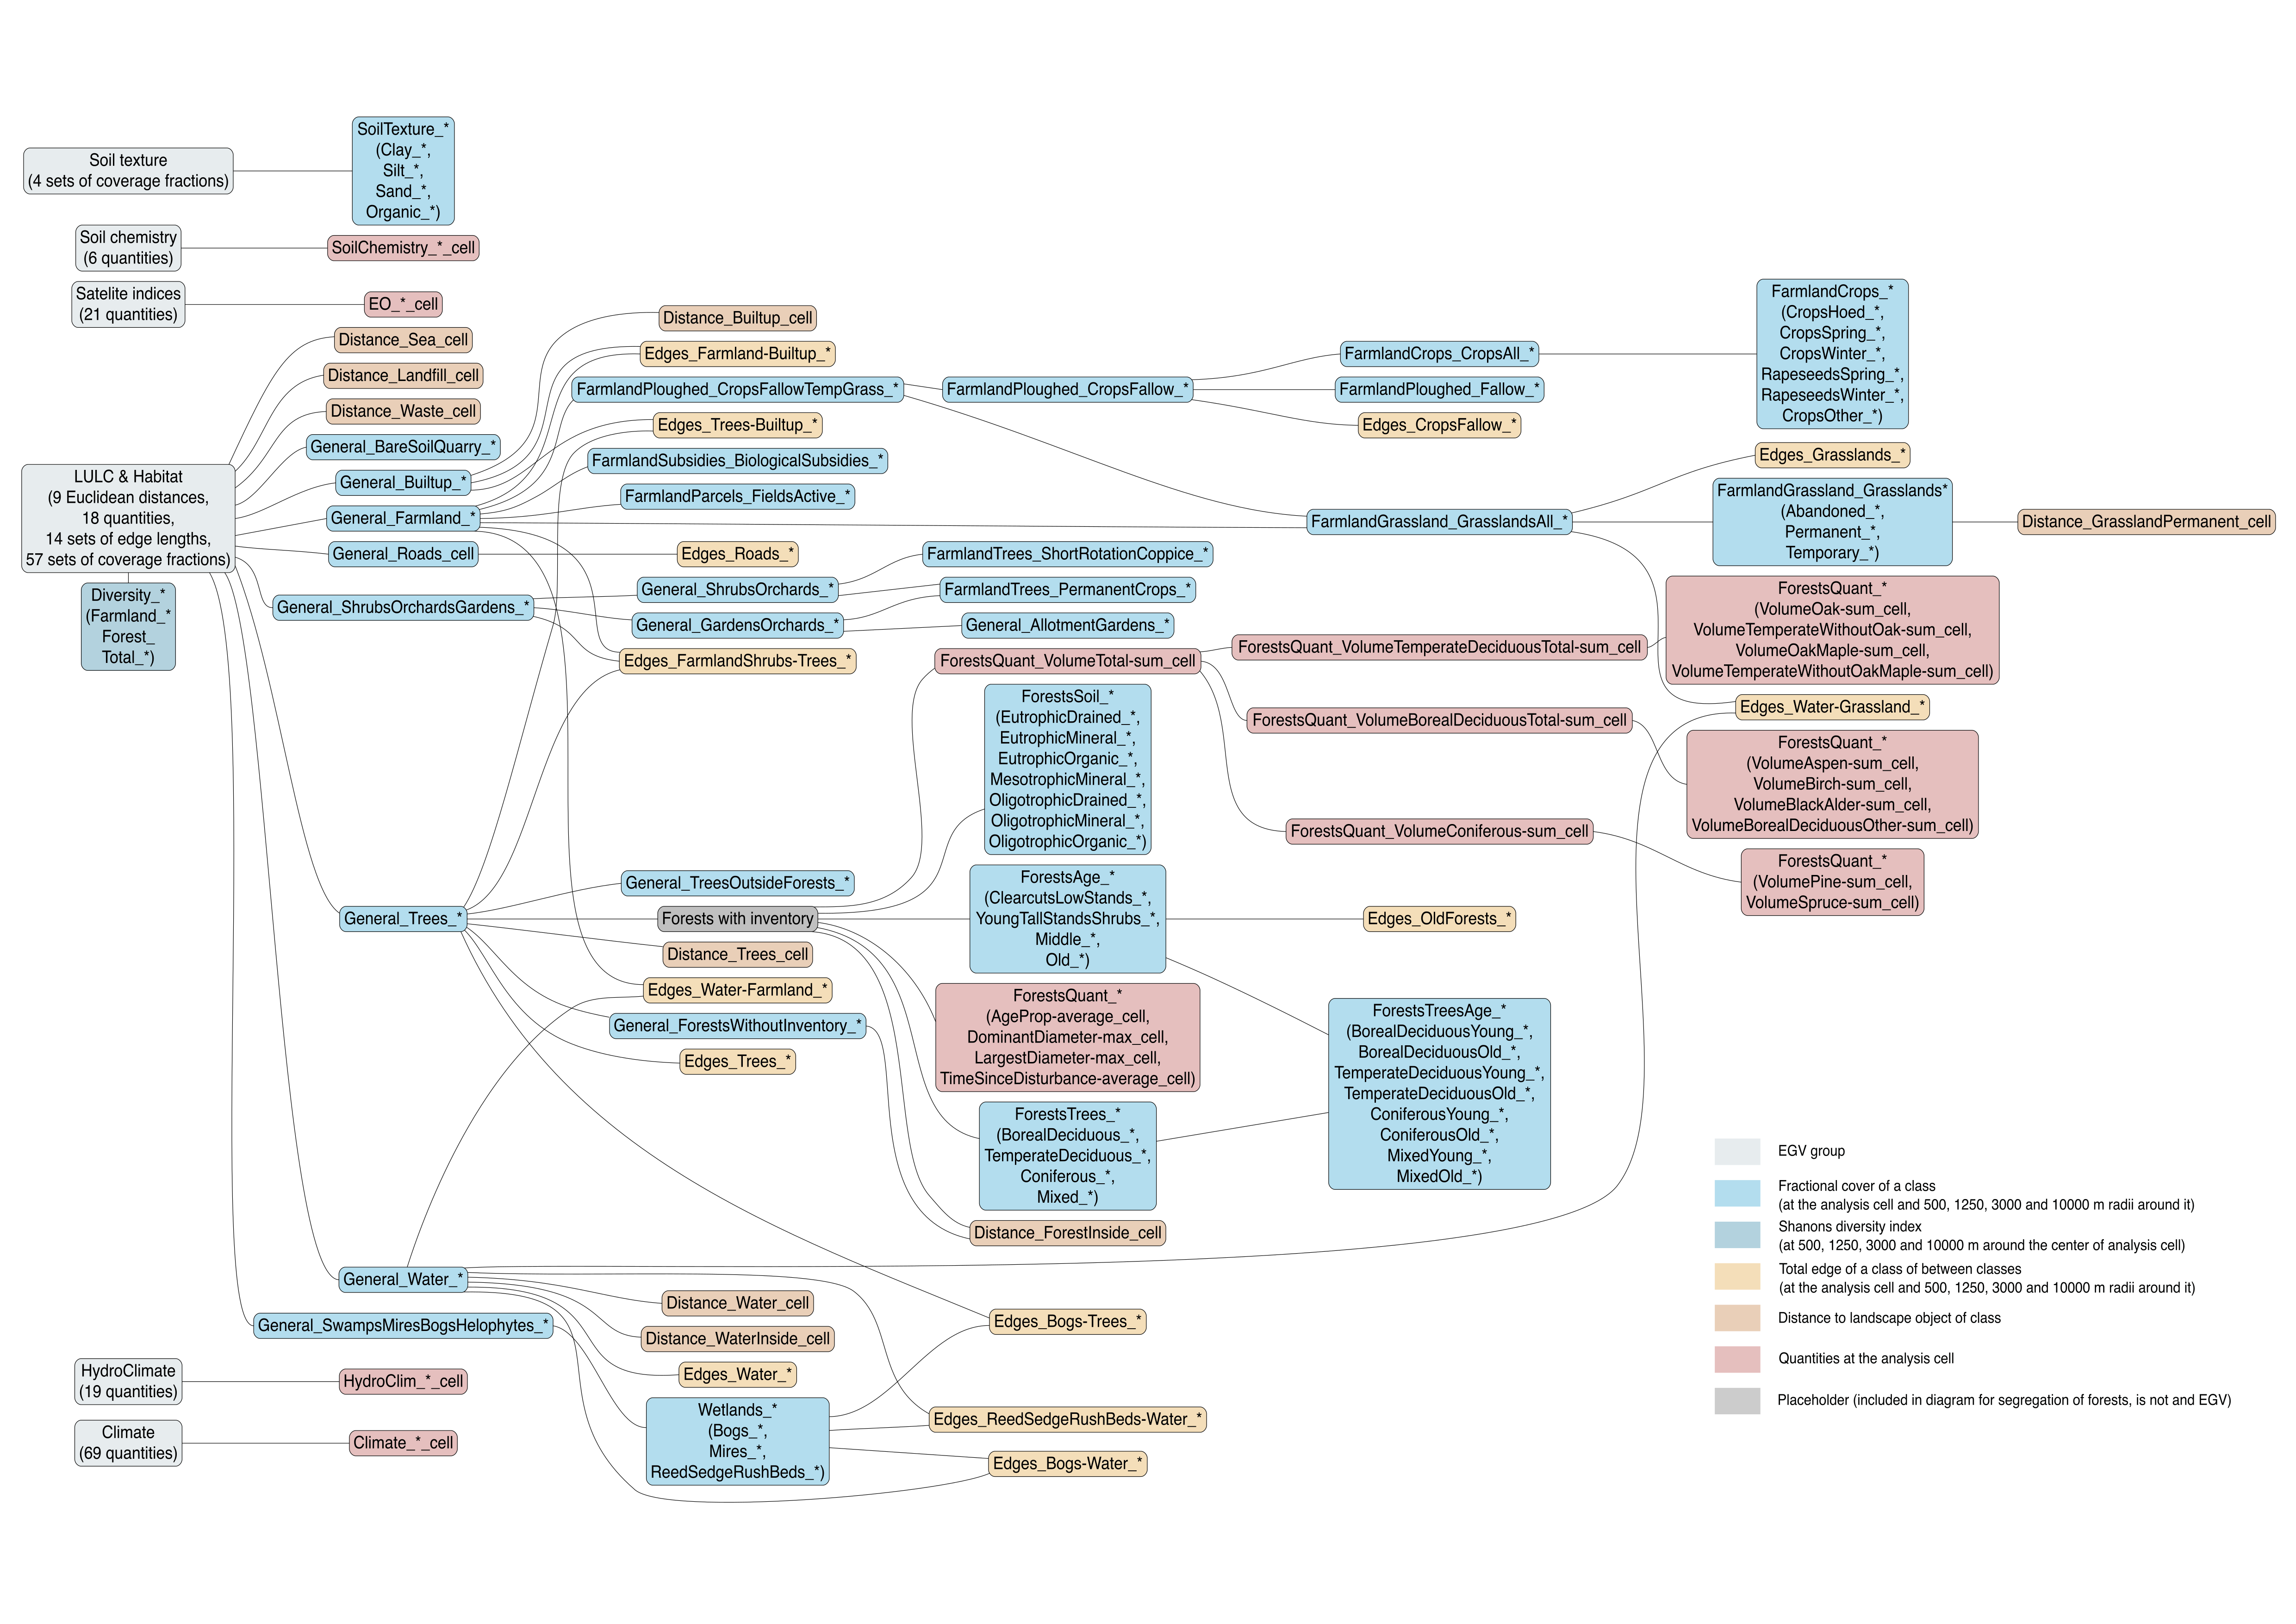
\includegraphics[width=1\linewidth]{./Figures/EGV_FlowChartY_eps_krasains_300dpi_2} \caption{Relationships of ecogeograpfical variables crated.}\label{fig:flowchart}
\end{figure}

In cover fraction and edge variables, we first calculated values at the analysis
cell resolution and then used \{exactextract\} to summarise values from larger scales.
This package uses pixel area weight to calculate weighted summary statistic, thus the
error created due to aggregation is negligible, particularly at larger scales, but
reduces computation time thousunds up to even hundreds of thousands times compared
to input resolution (10 m). To further speed up the procedures, we used ``sparse''
mode in \passthrough{\lstinline!egvtools::radius\_function!}, thus summarising zonal statistics every 300 m for
3000 m radius buffers and every 1000 m for 10000 m buffers, obtaining near linear
reduction in time relative to the number of zones (nine fold and 100 fold further
computation time reduction), while loosing less than 0.001 \% of variability altogether.

We used slightly different approach with diversity metrics - first we calculated
Shanons diversity index at 25 ha raster grid cells as there is nearly no variability
of landscape classes at 1 ha grid cells. Further on we calculated arithmetic mean as
zonal statictics value (``sparse'' mode with \passthrough{\lstinline!egvtools::radius\_function!}), but we
did not create this EGV at the analysis cells scale.

\section{Climate\_CHELSAv2.1-bio1\_cell}\label{ch06.001}

\textbf{filename:} \passthrough{\lstinline!Climate\_CHELSAv2.1-bio1\_cell.tif!}

\textbf{layername:} \passthrough{\lstinline!egv\_1!}

\textbf{English name:} Mean annual daily mean air temperature (°C) (CHELSA v2.1) within the analysis cell (1 ha)

\textbf{Latvian name:} Vidējā ikdienas gaisa temperatūra (°C) (CHELSA v2.1) analīzes šūnā (1 ha)

\textbf{Procedure:} Directly follows \hyperref[Ch04.11]{CHELSA v2.1}. EGV is prepared with the
workflow \passthrough{\lstinline!egvtools::downscale2egv()!} with inverse distance weighted (power = 2)
gap filling and soft smoothing (power = 0.5) over 5 km radius of every cell.

\begin{lstlisting}[language=R]
# libs ----
if(!require(egvtools)) {remotes::install_github("aavotins/egvtools"); require(egvtools)}

# job ----

localname="Climate_CHELSAv2.1-bio1_cell.tif"
layername="egv_1"
reading="./Geodata/2024/CHELSA/Climate_CHELSAv2.1-bio1_cell.tif"

df <- downscale2egv(
  template_path = "./Templates/TemplateRasters/LV100m_10km.tif",
  grid_path     = "./Templates/TemplateGrids/tikls1km_sauzeme.parquet",
  rawfile_path  = reading,
  out_path      = "./RasterGrids_100m/2024/RAW/",
  file_name     = localname,
  layer_name    = layername,
  fill_gaps     = TRUE,
  smooth        = TRUE,
  smooth_radius_km = 5,
  plot_result   = TRUE)
print(df)
\end{lstlisting}

\section{Climate\_CHELSAv2.1-bio10\_cell}\label{ch06.002}

\textbf{filename:} \passthrough{\lstinline!Climate\_CHELSAv2.1-bio10\_cell.tif!}

\textbf{layername:} \passthrough{\lstinline!egv\_2!}

\textbf{English name:} Mean daily mean air temperatures (°C) of the warmest quarter (CHELSA v2.1) within the analysis cell (1 ha)

\textbf{Latvian name:} Gada siltākā ceturkšņa vidējā gaisa temperatūra (°C) (CHELSA v2.1) analīzes šūnā (1 ha)

\textbf{Procedure:} Directly follows \hyperref[Ch04.11]{CHELSA v2.1}. EGV is prepared with the
workflow \passthrough{\lstinline!egvtools::downscale2egv()!} with inverse distance weighted (power = 2)
gap filling and soft smoothing (power = 0.5) over 5 km radius of every cell.

\begin{lstlisting}[language=R]
# libs ----
if(!require(egvtools)) {remotes::install_github("aavotins/egvtools"); require(egvtools)}

# job ----

localname="Climate_CHELSAv2.1-bio10_cell.tif"
layername="egv_2"
reading="./Geodata/2024/CHELSA/Climate_CHELSAv2.1-bio10_cell.tif"

df <- downscale2egv(
  template_path = "./Templates/TemplateRasters/LV100m_10km.tif",
  grid_path     = "./Templates/TemplateGrids/tikls1km_sauzeme.parquet",
  rawfile_path  = reading,
  out_path      = "./RasterGrids_100m/2024/RAW/",
  file_name     = localname,
  layer_name    = layername,
  fill_gaps     = TRUE,
  smooth        = TRUE,
  smooth_radius_km = 5,
  plot_result   = TRUE)
print(df)
\end{lstlisting}

\section{Climate\_CHELSAv2.1-bio11\_cell}\label{ch06.003}

\textbf{filename:} \passthrough{\lstinline!Climate\_CHELSAv2.1-bio11\_cell.tif!}

\textbf{layername:} \passthrough{\lstinline!egv\_3!}

\textbf{English name:} Mean daily mean air temperatures (°C) of the coldest quarter (CHELSA v2.1) within the analysis cell (1 ha)

\textbf{Latvian name:} Gada aukstākā ceturkšņa vidējā gaisa temperatūra (°C) (CHELSA v2.1) analīzes šūnā (1 ha)

\textbf{Procedure:} Directly follows \hyperref[Ch04.11]{CHELSA v2.1}. EGV is prepared with the
workflow \passthrough{\lstinline!egvtools::downscale2egv()!} with inverse distance weighted (power = 2)
gap filling and soft smoothing (power = 0.5) over 5 km radius of every cell.

\begin{lstlisting}[language=R]
# libs ----
if(!require(egvtools)) {remotes::install_github("aavotins/egvtools"); require(egvtools)}

# job ----

localname="Climate_CHELSAv2.1-bio11_cell.tif"
layername="egv_3"
reading="./Geodata/2024/CHELSA/Climate_CHELSAv2.1-bio11_cell.tif"

df <- downscale2egv(
  template_path = "./Templates/TemplateRasters/LV100m_10km.tif",
  grid_path     = "./Templates/TemplateGrids/tikls1km_sauzeme.parquet",
  rawfile_path  = reading,
  out_path      = "./RasterGrids_100m/2024/RAW/",
  file_name     = localname,
  layer_name    = layername,
  fill_gaps     = TRUE,
  smooth        = TRUE,
  smooth_radius_km = 5,
  plot_result   = TRUE)
print(df)
\end{lstlisting}

\section{Climate\_CHELSAv2.1-bio12\_cell}\label{ch06.004}

\textbf{filename:} \passthrough{\lstinline!Climate\_CHELSAv2.1-bio12\_cell.tif!}

\textbf{layername:} \passthrough{\lstinline!egv\_4!}

\textbf{English name:} Annual precipitation amount (kg m⁻² year⁻¹) (CHELSA v2.1) within the analysis cell (1 ha)

\textbf{Latvian name:} Gada nokrišņu daudzums (kg m⁻² gadā) (CHELSA v2.1) analīzes šūnā (1 ha)

\textbf{Procedure:} Directly follows \hyperref[Ch04.11]{CHELSA v2.1}. EGV is prepared with the
workflow \passthrough{\lstinline!egvtools::downscale2egv()!} with inverse distance weighted (power = 2)
gap filling and soft smoothing (power = 0.5) over 5 km radius of every cell.

\begin{lstlisting}[language=R]
# libs ----
if(!require(egvtools)) {remotes::install_github("aavotins/egvtools"); require(egvtools)}

# job ----

localname="Climate_CHELSAv2.1-bio12_cell.tif"
layername="egv_4"
reading="./Geodata/2024/CHELSA/Climate_CHELSAv2.1-bio12_cell.tif"

df <- downscale2egv(
  template_path = "./Templates/TemplateRasters/LV100m_10km.tif",
  grid_path     = "./Templates/TemplateGrids/tikls1km_sauzeme.parquet",
  rawfile_path  = reading,
  out_path      = "./RasterGrids_100m/2024/RAW/",
  file_name     = localname,
  layer_name    = layername,
  fill_gaps     = TRUE,
  smooth        = TRUE,
  smooth_radius_km = 5,
  plot_result   = TRUE)
print(df)
\end{lstlisting}

\section{Climate\_CHELSAv2.1-bio13\_cell}\label{ch06.005}

\textbf{filename:} \passthrough{\lstinline!Climate\_CHELSAv2.1-bio13\_cell.tif!}

\textbf{layername:} \passthrough{\lstinline!egv\_5!}

\textbf{English name:} Precipitation amount (kg m⁻² month⁻¹) of the wettest month (CHELSA v2.1) within the analysis cell (1 ha)

\textbf{Latvian name:} Slapjākā mēneša nokrišņu daudzums (kg m⁻² mēnesī) (CHELSA v2.1) analīzes šūnā (1 ha)

\textbf{Procedure:} Directly follows \hyperref[Ch04.11]{CHELSA v2.1}. EGV is prepared with the
workflow \passthrough{\lstinline!egvtools::downscale2egv()!} with inverse distance weighted (power = 2)
gap filling and soft smoothing (power = 0.5) over 5 km radius of every cell.

\begin{lstlisting}[language=R]
# libs ----
if(!require(egvtools)) {remotes::install_github("aavotins/egvtools"); require(egvtools)}

# job ----

localname="Climate_CHELSAv2.1-bio13_cell.tif"
layername="egv_5"
reading="./Geodata/2024/CHELSA/Climate_CHELSAv2.1-bio13_cell.tif"

df <- downscale2egv(
  template_path = "./Templates/TemplateRasters/LV100m_10km.tif",
  grid_path     = "./Templates/TemplateGrids/tikls1km_sauzeme.parquet",
  rawfile_path  = reading,
  out_path      = "./RasterGrids_100m/2024/RAW/",
  file_name     = localname,
  layer_name    = layername,
  fill_gaps     = TRUE,
  smooth        = TRUE,
  smooth_radius_km = 5,
  plot_result   = TRUE)
print(df)
\end{lstlisting}

\section{Climate\_CHELSAv2.1-bio14\_cell}\label{ch06.006}

\textbf{filename:} \passthrough{\lstinline!Climate\_CHELSAv2.1-bio14\_cell.tif!}

\textbf{layername:} \passthrough{\lstinline!egv\_6!}

\textbf{English name:} Precipitation amount (kg m⁻² month⁻¹) of the driest month (CHELSA v2.1) within the analysis cell (1 ha)

\textbf{Latvian name:} Sausākā mēneša nokrišņu daudzums (kg m⁻² mēnesī) (CHELSA v2.1) analīzes šūnā (1 ha)

\textbf{Procedure:} Directly follows \hyperref[Ch04.11]{CHELSA v2.1}. EGV is prepared with the
workflow \passthrough{\lstinline!egvtools::downscale2egv()!} with inverse distance weighted (power = 2)
gap filling and soft smoothing (power = 0.5) over 5 km radius of every cell.

\begin{lstlisting}[language=R]
# libs ----
if(!require(egvtools)) {remotes::install_github("aavotins/egvtools"); require(egvtools)}

# job ----

localname="Climate_CHELSAv2.1-bio14_cell.tif"
layername="egv_6"
reading="./Geodata/2024/CHELSA/Climate_CHELSAv2.1-bio14_cell.tif"

df <- downscale2egv(
  template_path = "./Templates/TemplateRasters/LV100m_10km.tif",
  grid_path     = "./Templates/TemplateGrids/tikls1km_sauzeme.parquet",
  rawfile_path  = reading,
  out_path      = "./RasterGrids_100m/2024/RAW/",
  file_name     = localname,
  layer_name    = layername,
  fill_gaps     = TRUE,
  smooth        = TRUE,
  smooth_radius_km = 5,
  plot_result   = TRUE)
print(df)
\end{lstlisting}

\section{Climate\_CHELSAv2.1-bio15\_cell}\label{ch06.007}

\textbf{filename:} \passthrough{\lstinline!Climate\_CHELSAv2.1-bio15\_cell.tif!}

\textbf{layername:} \passthrough{\lstinline!egv\_7!}

\textbf{English name:} Precipitation seasonality (kg m⁻²) (CHELSA v2.1) within the analysis cell (1 ha)

\textbf{Latvian name:} Nokrišņu sezonalitāte (kg m⁻²) (CHELSA v2.1) analīzes šūnā (1 ha)

\textbf{Procedure:} Directly follows \hyperref[Ch04.11]{CHELSA v2.1}. EGV is prepared with the
workflow \passthrough{\lstinline!egvtools::downscale2egv()!} with inverse distance weighted (power = 2)
gap filling and soft smoothing (power = 0.5) over 5 km radius of every cell.

\begin{lstlisting}[language=R]
# libs ----
if(!require(egvtools)) {remotes::install_github("aavotins/egvtools"); require(egvtools)}

# job ----

localname="Climate_CHELSAv2.1-bio15_cell.tif"
layername="egv_7"
reading="./Geodata/2024/CHELSA/Climate_CHELSAv2.1-bio15_cell.tif"

df <- downscale2egv(
  template_path = "./Templates/TemplateRasters/LV100m_10km.tif",
  grid_path     = "./Templates/TemplateGrids/tikls1km_sauzeme.parquet",
  rawfile_path  = reading,
  out_path      = "./RasterGrids_100m/2024/RAW/",
  file_name     = localname,
  layer_name    = layername,
  fill_gaps     = TRUE,
  smooth        = TRUE,
  smooth_radius_km = 5,
  plot_result   = TRUE)
print(df)
\end{lstlisting}

\section{Climate\_CHELSAv2.1-bio16\_cell}\label{ch06.008}

\textbf{filename:} \passthrough{\lstinline!Climate\_CHELSAv2.1-bio16\_cell.tif!}

\textbf{layername:} \passthrough{\lstinline!egv\_8!}

\textbf{English name:} Mean monthly precipitation amount (kg m⁻² month⁻¹) of the wettest quarter (CHELSA v2.1) within the analysis cell (1 ha)

\textbf{Latvian name:} Slapjākā ceturkšņa vidējais nokrišņu daudzums mēnesī (kg m⁻² mēnesī) (CHELSA v2.1) analīzes šūnā (1 ha)

\textbf{Procedure:} Directly follows \hyperref[Ch04.11]{CHELSA v2.1}. EGV is prepared with the
workflow \passthrough{\lstinline!egvtools::downscale2egv()!} with inverse distance weighted (power = 2)
gap filling and soft smoothing (power = 0.5) over 5 km radius of every cell.

\begin{lstlisting}[language=R]
# libs ----
if(!require(egvtools)) {remotes::install_github("aavotins/egvtools"); require(egvtools)}

# job ----

localname="Climate_CHELSAv2.1-bio16_cell.tif"
layername="egv_8"
reading="./Geodata/2024/CHELSA/Climate_CHELSAv2.1-bio16_cell.tif"

df <- downscale2egv(
  template_path = "./Templates/TemplateRasters/LV100m_10km.tif",
  grid_path     = "./Templates/TemplateGrids/tikls1km_sauzeme.parquet",
  rawfile_path  = reading,
  out_path      = "./RasterGrids_100m/2024/RAW/",
  file_name     = localname,
  layer_name    = layername,
  fill_gaps     = TRUE,
  smooth        = TRUE,
  smooth_radius_km = 5,
  plot_result   = TRUE)
print(df)
\end{lstlisting}

\section{Climate\_CHELSAv2.1-bio17\_cell}\label{ch06.009}

\textbf{filename:} \passthrough{\lstinline!Climate\_CHELSAv2.1-bio17\_cell.tif!}

\textbf{layername:} \passthrough{\lstinline!egv\_9!}

\textbf{English name:} Mean monthly precipitation amount (kg m⁻² month⁻¹) of the driest quarter (CHELSA v2.1) within the analysis cell (1 ha)

\textbf{Latvian name:} Sausākā ceturkšņa vidējais nokrišņu daudzums mēnesī (kg m⁻² mēnesī) (CHELSA v2.1) analīzes šūnā (1 ha)

\textbf{Procedure:} Directly follows \hyperref[Ch04.11]{CHELSA v2.1}. EGV is prepared with the
workflow \passthrough{\lstinline!egvtools::downscale2egv()!} with inverse distance weighted (power = 2)
gap filling and soft smoothing (power = 0.5) over 5 km radius of every cell.

\begin{lstlisting}[language=R]
# libs ----
if(!require(egvtools)) {remotes::install_github("aavotins/egvtools"); require(egvtools)}

# job ----

localname="Climate_CHELSAv2.1-bio17_cell.tif"
layername="egv_9"
reading="./Geodata/2024/CHELSA/Climate_CHELSAv2.1-bio17_cell.tif"

df <- downscale2egv(
  template_path = "./Templates/TemplateRasters/LV100m_10km.tif",
  grid_path     = "./Templates/TemplateGrids/tikls1km_sauzeme.parquet",
  rawfile_path  = reading,
  out_path      = "./RasterGrids_100m/2024/RAW/",
  file_name     = localname,
  layer_name    = layername,
  fill_gaps     = TRUE,
  smooth        = TRUE,
  smooth_radius_km = 5,
  plot_result   = TRUE)
print(df)
\end{lstlisting}

\section{Climate\_CHELSAv2.1-bio18\_cell}\label{ch06.010}

\textbf{filename:} \passthrough{\lstinline!Climate\_CHELSAv2.1-bio18\_cell.tif!}

\textbf{layername:} \passthrough{\lstinline!egv\_10!}

\textbf{English name:} Mean monthly precipitation amount (kg m⁻² month⁻¹) of the warmest quarter (CHELSA v2.1) within the analysis cell (1 ha)

\textbf{Latvian name:} Siltākā ceturkšņa vidējais nokrišņu daudzuma mēnesī (kg m⁻² mēnesī) (CHELSA v2.1) analīzes šūnā (1 ha)

\textbf{Procedure:} Directly follows \hyperref[Ch04.11]{CHELSA v2.1}. EGV is prepared with the
workflow \passthrough{\lstinline!egvtools::downscale2egv()!} with inverse distance weighted (power = 2)
gap filling and soft smoothing (power = 0.5) over 5 km radius of every cell.

\begin{lstlisting}[language=R]
# libs ----
if(!require(egvtools)) {remotes::install_github("aavotins/egvtools"); require(egvtools)}

# job ----

localname="Climate_CHELSAv2.1-bio18_cell.tif"
layername="egv_10"
reading="./Geodata/2024/CHELSA/Climate_CHELSAv2.1-bio18_cell.tif"

df <- downscale2egv(
  template_path = "./Templates/TemplateRasters/LV100m_10km.tif",
  grid_path     = "./Templates/TemplateGrids/tikls1km_sauzeme.parquet",
  rawfile_path  = reading,
  out_path      = "./RasterGrids_100m/2024/RAW/",
  file_name     = localname,
  layer_name    = layername,
  fill_gaps     = TRUE,
  smooth        = TRUE,
  smooth_radius_km = 5,
  plot_result   = TRUE)
print(df)
\end{lstlisting}

\section{Climate\_CHELSAv2.1-bio19\_cell}\label{ch06.011}

\textbf{filename:} \passthrough{\lstinline!Climate\_CHELSAv2.1-bio19\_cell.tif!}

\textbf{layername:} \passthrough{\lstinline!egv\_11!}

\textbf{English name:} Mean monthly precipitation amount (kg m⁻² month⁻¹) of the coldest quarter (CHELSA v2.1) within the analysis cell (1 ha)

\textbf{Latvian name:} Aukstākā ceturkšņa vidējais nokrišņu daudzums mēnesī (kg m⁻² mēnesī) (CHELSA v2.1) analīzes šūnā (1 ha)

\textbf{Procedure:} Directly follows \hyperref[Ch04.11]{CHELSA v2.1}. EGV is prepared with the
workflow \passthrough{\lstinline!egvtools::downscale2egv()!} with inverse distance weighted (power = 2)
gap filling and soft smoothing (power = 0.5) over 5 km radius of every cell.

\begin{lstlisting}[language=R]
# libs ----
if(!require(egvtools)) {remotes::install_github("aavotins/egvtools"); require(egvtools)}

# job ----

localname="Climate_CHELSAv2.1-bio19_cell.tif"
layername="egv_11"
reading="./Geodata/2024/CHELSA/Climate_CHELSAv2.1-bio19_cell.tif"

df <- downscale2egv(
  template_path = "./Templates/TemplateRasters/LV100m_10km.tif",
  grid_path     = "./Templates/TemplateGrids/tikls1km_sauzeme.parquet",
  rawfile_path  = reading,
  out_path      = "./RasterGrids_100m/2024/RAW/",
  file_name     = localname,
  layer_name    = layername,
  fill_gaps     = TRUE,
  smooth        = TRUE,
  smooth_radius_km = 5,
  plot_result   = TRUE)
print(df)
\end{lstlisting}

\section{Climate\_CHELSAv2.1-bio2\_cell}\label{ch06.012}

\textbf{filename:} \passthrough{\lstinline!Climate\_CHELSAv2.1-bio2\_cell.tif!}

\textbf{layername:} \passthrough{\lstinline!egv\_12!}

\textbf{English name:} Mean diurnal air temperature range (°C) (CHELSA v2.1) within the analysis cell (1 ha)

\textbf{Latvian name:} Diennakts temperatūru amplitūda (°C) (CHELSA v2.1) analīzes šūnā (1 ha)

\textbf{Procedure:} Directly follows \hyperref[Ch04.11]{CHELSA v2.1}. EGV is prepared with the
workflow \passthrough{\lstinline!egvtools::downscale2egv()!} with inverse distance weighted (power = 2)
gap filling and soft smoothing (power = 0.5) over 5 km radius of every cell.

\begin{lstlisting}[language=R]
# libs ----
if(!require(egvtools)) {remotes::install_github("aavotins/egvtools"); require(egvtools)}

# job ----

localname="Climate_CHELSAv2.1-bio2_cell.tif"
layername="egv_12"
reading="./Geodata/2024/CHELSA/Climate_CHELSAv2.1-bio2_cell.tif"

df <- downscale2egv(
  template_path = "./Templates/TemplateRasters/LV100m_10km.tif",
  grid_path     = "./Templates/TemplateGrids/tikls1km_sauzeme.parquet",
  rawfile_path  = reading,
  out_path      = "./RasterGrids_100m/2024/RAW/",
  file_name     = localname,
  layer_name    = layername,
  fill_gaps     = TRUE,
  smooth        = TRUE,
  smooth_radius_km = 5,
  plot_result   = TRUE)
print(df)
\end{lstlisting}

\section{Climate\_CHELSAv2.1-bio3\_cell}\label{ch06.013}

\textbf{filename:} \passthrough{\lstinline!Climate\_CHELSAv2.1-bio3\_cell.tif!}

\textbf{layername:} \passthrough{\lstinline!egv\_13!}

\textbf{English name:} Isothermality (ratio of diurnal variation to annual variation in temperatures) (°C) (CHELSA v2.1) within the analysis cell (1 ha)

\textbf{Latvian name:} Izotermalitāte (attiecība starp diennakts un gada temperatūras svārstībām) (°C) (CHELSA v2.1) analīzes šūnā (1 ha)

\textbf{Procedure:} Directly follows \hyperref[Ch04.11]{CHELSA v2.1}. EGV is prepared with the
workflow \passthrough{\lstinline!egvtools::downscale2egv()!} with inverse distance weighted (power = 2)
gap filling and soft smoothing (power = 0.5) over 5 km radius of every cell.

\begin{lstlisting}[language=R]
# libs ----
if(!require(egvtools)) {remotes::install_github("aavotins/egvtools"); require(egvtools)}

# job ----

localname="Climate_CHELSAv2.1-bio3_cell.tif"
layername="egv_13"
reading="./Geodata/2024/CHELSA/Climate_CHELSAv2.1-bio3_cell.tif"

df <- downscale2egv(
  template_path = "./Templates/TemplateRasters/LV100m_10km.tif",
  grid_path     = "./Templates/TemplateGrids/tikls1km_sauzeme.parquet",
  rawfile_path  = reading,
  out_path      = "./RasterGrids_100m/2024/RAW/",
  file_name     = localname,
  layer_name    = layername,
  fill_gaps     = TRUE,
  smooth        = TRUE,
  smooth_radius_km = 5,
  plot_result   = TRUE)
print(df)
\end{lstlisting}

\section{Climate\_CHELSAv2.1-bio4\_cell}\label{ch06.014}

\textbf{filename:} \passthrough{\lstinline!Climate\_CHELSAv2.1-bio4\_cell.tif!}

\textbf{layername:} \passthrough{\lstinline!egv\_14!}

\textbf{English name:} Temperature seasonality (standard deviation of the monthly mean temperatures) (°C/100) (CHELSA v2.1) within the analysis cell (1 ha)

\textbf{Latvian name:} Temperatūru sezonalitāte (mēneša vidējo temperatūru standartnovirze) (°C/100) (CHELSA v2.1) analīzes šūnā (1 ha)

\textbf{Procedure:} Directly follows \hyperref[Ch04.11]{CHELSA v2.1}. EGV is prepared with the
workflow \passthrough{\lstinline!egvtools::downscale2egv()!} with inverse distance weighted (power = 2)
gap filling and soft smoothing (power = 0.5) over 5 km radius of every cell.

\begin{lstlisting}[language=R]
# libs ----
if(!require(egvtools)) {remotes::install_github("aavotins/egvtools"); require(egvtools)}

# job ----

localname="Climate_CHELSAv2.1-bio4_cell.tif"
layername="egv_14"
reading="./Geodata/2024/CHELSA/Climate_CHELSAv2.1-bio4_cell.tif"

df <- downscale2egv(
  template_path = "./Templates/TemplateRasters/LV100m_10km.tif",
  grid_path     = "./Templates/TemplateGrids/tikls1km_sauzeme.parquet",
  rawfile_path  = reading,
  out_path      = "./RasterGrids_100m/2024/RAW/",
  file_name     = localname,
  layer_name    = layername,
  fill_gaps     = TRUE,
  smooth        = TRUE,
  smooth_radius_km = 5,
  plot_result   = TRUE)
print(df)
\end{lstlisting}

\section{Climate\_CHELSAv2.1-bio5\_cell}\label{ch06.015}

\textbf{filename:} \passthrough{\lstinline!Climate\_CHELSAv2.1-bio5\_cell.tif!}

\textbf{layername:} \passthrough{\lstinline!egv\_15!}

\textbf{English name:} Mean daily maximum air temperature (°C) of the warmest month (CHELSA v2.1) within the analysis cell (1 ha)

\textbf{Latvian name:} Siltākā mēneša vidējā ikdienas augstākā gaisa temperatūra (°C) (CHELSA v2.1) analīzes šūnā (1 ha)

\textbf{Procedure:} Directly follows \hyperref[Ch04.11]{CHELSA v2.1}. EGV is prepared with the
workflow \passthrough{\lstinline!egvtools::downscale2egv()!} with inverse distance weighted (power = 2)
gap filling and soft smoothing (power = 0.5) over 5 km radius of every cell.

\begin{lstlisting}[language=R]
# libs ----
if(!require(egvtools)) {remotes::install_github("aavotins/egvtools"); require(egvtools)}

# job ----

localname="Climate_CHELSAv2.1-bio5_cell.tif"
layername="egv_15"
reading="./Geodata/2024/CHELSA/Climate_CHELSAv2.1-bio5_cell.tif"

df <- downscale2egv(
  template_path = "./Templates/TemplateRasters/LV100m_10km.tif",
  grid_path     = "./Templates/TemplateGrids/tikls1km_sauzeme.parquet",
  rawfile_path  = reading,
  out_path      = "./RasterGrids_100m/2024/RAW/",
  file_name     = localname,
  layer_name    = layername,
  fill_gaps     = TRUE,
  smooth        = TRUE,
  smooth_radius_km = 5,
  plot_result   = TRUE)
print(df)
\end{lstlisting}

\section{Climate\_CHELSAv2.1-bio6\_cell}\label{ch06.016}

\textbf{filename:} \passthrough{\lstinline!Climate\_CHELSAv2.1-bio6\_cell.tif!}

\textbf{layername:} \passthrough{\lstinline!egv\_16!}

\textbf{English name:} Mean daily minimum air temperature (°C) of the coldest month (CHELSA v2.1) within the analysis cell (1 ha)

\textbf{Latvian name:} Aukstākā mēneša vidējā ikdienas zemākā gaisa temperatūra (°C) (CHELSA v2.1) analīzes šūnā (1 ha)

\textbf{Procedure:} Directly follows \hyperref[Ch04.11]{CHELSA v2.1}. EGV is prepared with the
workflow \passthrough{\lstinline!egvtools::downscale2egv()!} with inverse distance weighted (power = 2)
gap filling and soft smoothing (power = 0.5) over 5 km radius of every cell.

\begin{lstlisting}[language=R]
# libs ----
if(!require(egvtools)) {remotes::install_github("aavotins/egvtools"); require(egvtools)}

# job ----

localname="Climate_CHELSAv2.1-bio6_cell.tif"
layername="egv_16"
reading="./Geodata/2024/CHELSA/Climate_CHELSAv2.1-bio6_cell.tif"

df <- downscale2egv(
  template_path = "./Templates/TemplateRasters/LV100m_10km.tif",
  grid_path     = "./Templates/TemplateGrids/tikls1km_sauzeme.parquet",
  rawfile_path  = reading,
  out_path      = "./RasterGrids_100m/2024/RAW/",
  file_name     = localname,
  layer_name    = layername,
  fill_gaps     = TRUE,
  smooth        = TRUE,
  smooth_radius_km = 5,
  plot_result   = TRUE)
print(df)
\end{lstlisting}

\section{Climate\_CHELSAv2.1-bio7\_cell}\label{ch06.017}

\textbf{filename:} \passthrough{\lstinline!Climate\_CHELSAv2.1-bio7\_cell.tif!}

\textbf{layername:} \passthrough{\lstinline!egv\_17!}

\textbf{English name:} Annual range of air temperature (°C) (CHELSA v2.1) within the analysis cell (1 ha)

\textbf{Latvian name:} Gada temperatūru amplitūda (°C) (CHELSA v2.1) analīzes šūnā (1 ha)

\textbf{Procedure:} Directly follows \hyperref[Ch04.11]{CHELSA v2.1}. EGV is prepared with the
workflow \passthrough{\lstinline!egvtools::downscale2egv()!} with inverse distance weighted (power = 2)
gap filling and soft smoothing (power = 0.5) over 5 km radius of every cell.

\begin{lstlisting}[language=R]
# libs ----
if(!require(egvtools)) {remotes::install_github("aavotins/egvtools"); require(egvtools)}

# job ----

localname="Climate_CHELSAv2.1-bio7_cell.tif"
layername="egv_17"
reading="./Geodata/2024/CHELSA/Climate_CHELSAv2.1-bio7_cell.tif"

df <- downscale2egv(
  template_path = "./Templates/TemplateRasters/LV100m_10km.tif",
  grid_path     = "./Templates/TemplateGrids/tikls1km_sauzeme.parquet",
  rawfile_path  = reading,
  out_path      = "./RasterGrids_100m/2024/RAW/",
  file_name     = localname,
  layer_name    = layername,
  fill_gaps     = TRUE,
  smooth        = TRUE,
  smooth_radius_km = 5,
  plot_result   = TRUE)
print(df)
\end{lstlisting}

\section{Climate\_CHELSAv2.1-bio8\_cell}\label{ch06.018}

\textbf{filename:} \passthrough{\lstinline!Climate\_CHELSAv2.1-bio8\_cell.tif!}

\textbf{layername:} \passthrough{\lstinline!egv\_18!}

\textbf{English name:} Mean daily mean air temperatures (°C) of the wettest quarter (CHELSA v2.1) within the analysis cell (1 ha)

\textbf{Latvian name:} Slapjākā ceturkšņa vidējā ikdienas vidējā gaisa temperatūra (°C) (CHELSA v2.1) analīzes šūnā (1 ha)

\textbf{Procedure:} Directly follows \hyperref[Ch04.11]{CHELSA v2.1}. EGV is prepared with the
workflow \passthrough{\lstinline!egvtools::downscale2egv()!} with inverse distance weighted (power = 2)
gap filling and soft smoothing (power = 0.5) over 5 km radius of every cell.

\begin{lstlisting}[language=R]
# libs ----
if(!require(egvtools)) {remotes::install_github("aavotins/egvtools"); require(egvtools)}

# job ----

localname="Climate_CHELSAv2.1-bio8_cell.tif"
layername="egv_18"
reading="./Geodata/2024/CHELSA/Climate_CHELSAv2.1-bio8_cell.tif"

df <- downscale2egv(
  template_path = "./Templates/TemplateRasters/LV100m_10km.tif",
  grid_path     = "./Templates/TemplateGrids/tikls1km_sauzeme.parquet",
  rawfile_path  = reading,
  out_path      = "./RasterGrids_100m/2024/RAW/",
  file_name     = localname,
  layer_name    = layername,
  fill_gaps     = TRUE,
  smooth        = TRUE,
  smooth_radius_km = 5,
  plot_result   = TRUE)
print(df)
\end{lstlisting}

\section{Climate\_CHELSAv2.1-bio9\_cell}\label{ch06.019}

\textbf{filename:} \passthrough{\lstinline!Climate\_CHELSAv2.1-bio9\_cell.tif!}

\textbf{layername:} \passthrough{\lstinline!egv\_19!}

\textbf{English name:} Mean daily mean air temperatures (°C) of the driest quarter (CHELSA v2.1) within the analysis cell (1 ha)

\textbf{Latvian name:} Sausākā ceturkšņa vidējā ikdienas vidējā gaisa temperatūra (°C) (CHELSA v2.1) analīzes šūnā (1 ha)

\textbf{Procedure:} Directly follows \hyperref[Ch04.11]{CHELSA v2.1}. EGV is prepared with the
workflow \passthrough{\lstinline!egvtools::downscale2egv()!} with inverse distance weighted (power = 2)
gap filling and soft smoothing (power = 0.5) over 5 km radius of every cell.

\begin{lstlisting}[language=R]
# libs ----
if(!require(egvtools)) {remotes::install_github("aavotins/egvtools"); require(egvtools)}

# job ----

localname="Climate_CHELSAv2.1-bio9_cell.tif"
layername="egv_19"
reading="./Geodata/2024/CHELSA/Climate_CHELSAv2.1-bio9_cell.tif"

df <- downscale2egv(
  template_path = "./Templates/TemplateRasters/LV100m_10km.tif",
  grid_path     = "./Templates/TemplateGrids/tikls1km_sauzeme.parquet",
  rawfile_path  = reading,
  out_path      = "./RasterGrids_100m/2024/RAW/",
  file_name     = localname,
  layer_name    = layername,
  fill_gaps     = TRUE,
  smooth        = TRUE,
  smooth_radius_km = 5,
  plot_result   = TRUE)
print(df)
\end{lstlisting}

\section{Climate\_CHELSAv2.1-clt-max\_cell}\label{ch06.020}

\textbf{filename:} \passthrough{\lstinline!Climate\_CHELSAv2.1-clt-max\_cell.tif!}

\textbf{layername:} \passthrough{\lstinline!egv\_20!}

\textbf{English name:} Maximum monthly cloud area fraction (\%) (CHELSA v2.1) within the analysis cell (1 ha)

\textbf{Latvian name:} Maksimālais mēneša vidējais mākoņu segums (\%) (CHELSA v2.1) analīzes šūnā (1 ha)

\textbf{Procedure:} Directly follows \hyperref[Ch04.11]{CHELSA v2.1}. EGV is prepared with the
workflow \passthrough{\lstinline!egvtools::downscale2egv()!} with inverse distance weighted (power = 2)
gap filling and soft smoothing (power = 0.5) over 5 km radius of every cell.

\begin{lstlisting}[language=R]
# libs ----
if(!require(egvtools)) {remotes::install_github("aavotins/egvtools"); require(egvtools)}

# job ----

localname="Climate_CHELSAv2.1-clt-max_cell.tif"
layername="egv_20"
reading="./Geodata/2024/CHELSA/Climate_CHELSAv2.1-clt-max_cell.tif"

df <- downscale2egv(
  template_path = "./Templates/TemplateRasters/LV100m_10km.tif",
  grid_path     = "./Templates/TemplateGrids/tikls1km_sauzeme.parquet",
  rawfile_path  = reading,
  out_path      = "./RasterGrids_100m/2024/RAW/",
  file_name     = localname,
  layer_name    = layername,
  fill_gaps     = TRUE,
  smooth        = TRUE,
  smooth_radius_km = 5,
  plot_result   = TRUE)
print(df)
\end{lstlisting}

\section{Climate\_CHELSAv2.1-clt-mean\_cell}\label{ch06.021}

\textbf{filename:} \passthrough{\lstinline!Climate\_CHELSAv2.1-clt-mean\_cell.tif!}

\textbf{layername:} \passthrough{\lstinline!egv\_21!}

\textbf{English name:} Mean monthly cloud area fraction (\%) (CHELSA v2.1) within the analysis cell (1 ha)

\textbf{Latvian name:} Vidējais mākoņu segums (\%) (CHELSA v2.1) analīzes šūnā (1 ha)

\textbf{Procedure:} Directly follows \hyperref[Ch04.11]{CHELSA v2.1}. EGV is prepared with the
workflow \passthrough{\lstinline!egvtools::downscale2egv()!} with inverse distance weighted (power = 2)
gap filling and soft smoothing (power = 0.5) over 5 km radius of every cell.

\begin{lstlisting}[language=R]
# libs ----
if(!require(egvtools)) {remotes::install_github("aavotins/egvtools"); require(egvtools)}

# job ----

localname="Climate_CHELSAv2.1-clt-mean_cell.tif"
layername="egv_21"
reading="./Geodata/2024/CHELSA/Climate_CHELSAv2.1-clt-mean_cell.tif"

df <- downscale2egv(
  template_path = "./Templates/TemplateRasters/LV100m_10km.tif",
  grid_path     = "./Templates/TemplateGrids/tikls1km_sauzeme.parquet",
  rawfile_path  = reading,
  out_path      = "./RasterGrids_100m/2024/RAW/",
  file_name     = localname,
  layer_name    = layername,
  fill_gaps     = TRUE,
  smooth        = TRUE,
  smooth_radius_km = 5,
  plot_result   = TRUE)
print(df)
\end{lstlisting}

\section{Climate\_CHELSAv2.1-clt-min\_cell}\label{ch06.022}

\textbf{filename:} \passthrough{\lstinline!Climate\_CHELSAv2.1-clt-min\_cell.tif!}

\textbf{layername:} \passthrough{\lstinline!egv\_22!}

\textbf{English name:} Minimum monthly cloud area fraction (\%) (CHELSA v2.1) within the analysis cell (1 ha)

\textbf{Latvian name:} Minimālais mēneša vidējais mākoņu segums (\%) (CHELSA v2.1) analīzes šūnā (1 ha)

\textbf{Procedure:} Directly follows \hyperref[Ch04.11]{CHELSA v2.1}. EGV is prepared with the
workflow \passthrough{\lstinline!egvtools::downscale2egv()!} with inverse distance weighted (power = 2)
gap filling and soft smoothing (power = 0.5) over 5 km radius of every cell.

\begin{lstlisting}[language=R]
# libs ----
if(!require(egvtools)) {remotes::install_github("aavotins/egvtools"); require(egvtools)}

# job ----

localname="Climate_CHELSAv2.1-clt-min_cell.tif"
layername="egv_22"
reading="./Geodata/2024/CHELSA/Climate_CHELSAv2.1-clt-min_cell.tif"

df <- downscale2egv(
  template_path = "./Templates/TemplateRasters/LV100m_10km.tif",
  grid_path     = "./Templates/TemplateGrids/tikls1km_sauzeme.parquet",
  rawfile_path  = reading,
  out_path      = "./RasterGrids_100m/2024/RAW/",
  file_name     = localname,
  layer_name    = layername,
  fill_gaps     = TRUE,
  smooth        = TRUE,
  smooth_radius_km = 5,
  plot_result   = TRUE)
print(df)
\end{lstlisting}

\section{Climate\_CHELSAv2.1-clt-range\_cell}\label{ch06.023}

\textbf{filename:} \passthrough{\lstinline!Climate\_CHELSAv2.1-clt-range\_cell.tif!}

\textbf{layername:} \passthrough{\lstinline!egv\_23!}

\textbf{English name:} Annual range of monthly cloud area fraction (\%) (CHELSA v2.1) within the analysis cell (1 ha)

\textbf{Latvian name:} Gada mākoņu seguma amplitūda (\%) (CHELSA v2.1) analīzes šūnā (1 ha)

\textbf{Procedure:} Directly follows \hyperref[Ch04.11]{CHELSA v2.1}. EGV is prepared with the
workflow \passthrough{\lstinline!egvtools::downscale2egv()!} with inverse distance weighted (power = 2)
gap filling and soft smoothing (power = 0.5) over 5 km radius of every cell.

\begin{lstlisting}[language=R]
# libs ----
if(!require(egvtools)) {remotes::install_github("aavotins/egvtools"); require(egvtools)}

# job ----

localname="Climate_CHELSAv2.1-clt-range_cell.tif"
layername="egv_23"
reading="./Geodata/2024/CHELSA/Climate_CHELSAv2.1-clt-range_cell.tif"

df <- downscale2egv(
  template_path = "./Templates/TemplateRasters/LV100m_10km.tif",
  grid_path     = "./Templates/TemplateGrids/tikls1km_sauzeme.parquet",
  rawfile_path  = reading,
  out_path      = "./RasterGrids_100m/2024/RAW/",
  file_name     = localname,
  layer_name    = layername,
  fill_gaps     = TRUE,
  smooth        = TRUE,
  smooth_radius_km = 5,
  plot_result   = TRUE)
print(df)
\end{lstlisting}

\section{Climate\_CHELSAv2.1-cmi-max\_cell}\label{ch06.024}

\textbf{filename:} \passthrough{\lstinline!Climate\_CHELSAv2.1-cmi-max\_cell.tif!}

\textbf{layername:} \passthrough{\lstinline!egv\_24!}

\textbf{English name:} Maximum monthly climate moisture index (kg m⁻² month⁻¹) (CHELSA v2.1) within the analysis cell (1 ha)

\textbf{Latvian name:} Maksimālais mēneša vidējais klimata mitruma indekss (kg m⁻² month⁻¹) (CHELSA v2.1) analīzes šūnā (1 ha)

\textbf{Procedure:} Directly follows \hyperref[Ch04.11]{CHELSA v2.1}. EGV is prepared with the
workflow \passthrough{\lstinline!egvtools::downscale2egv()!} with inverse distance weighted (power = 2)
gap filling and soft smoothing (power = 0.5) over 5 km radius of every cell.

\begin{lstlisting}[language=R]
# libs ----
if(!require(egvtools)) {remotes::install_github("aavotins/egvtools"); require(egvtools)}

# job ----

localname="Climate_CHELSAv2.1-cmi-max_cell.tif"
layername="egv_24"
reading="./Geodata/2024/CHELSA/Climate_CHELSAv2.1-cmi-max_cell.tif"

df <- downscale2egv(
  template_path = "./Templates/TemplateRasters/LV100m_10km.tif",
  grid_path     = "./Templates/TemplateGrids/tikls1km_sauzeme.parquet",
  rawfile_path  = reading,
  out_path      = "./RasterGrids_100m/2024/RAW/",
  file_name     = localname,
  layer_name    = layername,
  fill_gaps     = TRUE,
  smooth        = TRUE,
  smooth_radius_km = 5,
  plot_result   = TRUE)
print(df)
\end{lstlisting}

\section{Climate\_CHELSAv2.1-cmi-mean\_cell}\label{ch06.025}

\textbf{filename:} \passthrough{\lstinline!Climate\_CHELSAv2.1-cmi-mean\_cell.tif!}

\textbf{layername:} \passthrough{\lstinline!egv\_25!}

\textbf{English name:} Mean monthly climate moisture index (kg m⁻² month⁻¹) (CHELSA v2.1) within the analysis cell (1 ha)

\textbf{Latvian name:} Vidējais klimata mitruma indekss (kg m⁻² month⁻¹) (CHELSA v2.1) analīzes šūnā (1 ha)

\textbf{Procedure:} Directly follows \hyperref[Ch04.11]{CHELSA v2.1}. EGV is prepared with the
workflow \passthrough{\lstinline!egvtools::downscale2egv()!} with inverse distance weighted (power = 2)
gap filling and soft smoothing (power = 0.5) over 5 km radius of every cell.

\begin{lstlisting}[language=R]
# libs ----
if(!require(egvtools)) {remotes::install_github("aavotins/egvtools"); require(egvtools)}

# job ----

localname="Climate_CHELSAv2.1-cmi-mean_cell.tif"
layername="egv_25"
reading="./Geodata/2024/CHELSA/Climate_CHELSAv2.1-cmi-mean_cell.tif"

df <- downscale2egv(
  template_path = "./Templates/TemplateRasters/LV100m_10km.tif",
  grid_path     = "./Templates/TemplateGrids/tikls1km_sauzeme.parquet",
  rawfile_path  = reading,
  out_path      = "./RasterGrids_100m/2024/RAW/",
  file_name     = localname,
  layer_name    = layername,
  fill_gaps     = TRUE,
  smooth        = TRUE,
  smooth_radius_km = 5,
  plot_result   = TRUE)
print(df)
\end{lstlisting}

\section{Climate\_CHELSAv2.1-cmi-min\_cell}\label{ch06.026}

\textbf{filename:} \passthrough{\lstinline!Climate\_CHELSAv2.1-cmi-min\_cell.tif!}

\textbf{layername:} \passthrough{\lstinline!egv\_26!}

\textbf{English name:} Minimum monthly climate moisture index (kg m⁻² month⁻¹) (CHELSA v2.1) within the analysis cell (1 ha)

\textbf{Latvian name:} Minimālais mēneša vidējais klimata mitruma indekss (kg m⁻² month⁻¹) (CHELSA v2.1) analīzes šūnā (1 ha)

\textbf{Procedure:} Directly follows \hyperref[Ch04.11]{CHELSA v2.1}. EGV is prepared with the
workflow \passthrough{\lstinline!egvtools::downscale2egv()!} with inverse distance weighted (power = 2)
gap filling and soft smoothing (power = 0.5) over 5 km radius of every cell.

\begin{lstlisting}[language=R]
# libs ----
if(!require(egvtools)) {remotes::install_github("aavotins/egvtools"); require(egvtools)}

# job ----

localname="Climate_CHELSAv2.1-cmi-min_cell.tif"
layername="egv_26"
reading="./Geodata/2024/CHELSA/Climate_CHELSAv2.1-cmi-min_cell.tif"

df <- downscale2egv(
  template_path = "./Templates/TemplateRasters/LV100m_10km.tif",
  grid_path     = "./Templates/TemplateGrids/tikls1km_sauzeme.parquet",
  rawfile_path  = reading,
  out_path      = "./RasterGrids_100m/2024/RAW/",
  file_name     = localname,
  layer_name    = layername,
  fill_gaps     = TRUE,
  smooth        = TRUE,
  smooth_radius_km = 5,
  plot_result   = TRUE)
print(df)
\end{lstlisting}

\section{Climate\_CHELSAv2.1-cmi-range\_cell}\label{ch06.027}

\textbf{filename:} \passthrough{\lstinline!Climate\_CHELSAv2.1-cmi-range\_cell.tif!}

\textbf{layername:} \passthrough{\lstinline!egv\_27!}

\textbf{English name:} Annual range of monthly climate moisture index (kg m⁻² month⁻¹) (CHELSA v2.1) within the analysis cell (1 ha)

\textbf{Latvian name:} Gada klimata mitruma indeksa amplitūda (kg m⁻² month⁻¹) (CHELSA v2.1) analīzes šūnā (1 ha)

\textbf{Procedure:} Directly follows \hyperref[Ch04.11]{CHELSA v2.1}. EGV is prepared with the
workflow \passthrough{\lstinline!egvtools::downscale2egv()!} with inverse distance weighted (power = 2)
gap filling and soft smoothing (power = 0.5) over 5 km radius of every cell.

\begin{lstlisting}[language=R]
# libs ----
if(!require(egvtools)) {remotes::install_github("aavotins/egvtools"); require(egvtools)}

# job ----

localname="Climate_CHELSAv2.1-cmi-range_cell.tif"
layername="egv_27"
reading="./Geodata/2024/CHELSA/Climate_CHELSAv2.1-cmi-range_cell.tif"

df <- downscale2egv(
  template_path = "./Templates/TemplateRasters/LV100m_10km.tif",
  grid_path     = "./Templates/TemplateGrids/tikls1km_sauzeme.parquet",
  rawfile_path  = reading,
  out_path      = "./RasterGrids_100m/2024/RAW/",
  file_name     = localname,
  layer_name    = layername,
  fill_gaps     = TRUE,
  smooth        = TRUE,
  smooth_radius_km = 5,
  plot_result   = TRUE)
print(df)
\end{lstlisting}

\section{Climate\_CHELSAv2.1-fcf\_cell}\label{ch06.028}

\textbf{filename:} \passthrough{\lstinline!Climate\_CHELSAv2.1-fcf\_cell.tif!}

\textbf{layername:} \passthrough{\lstinline!egv\_28!}

\textbf{English name:} Frost change frequency (number of events in which tmin or tmax go above or below 0°C) (CHELSA v2.1) within the analysis cell (1 ha)

\textbf{Latvian name:} Sasalšanas gadījumu biežums (zemākā vai augstākā temperatūra šķērso 0°C) (CHELSA v2.1) analīzes šūnā (1 ha)

\textbf{Procedure:} Directly follows \hyperref[Ch04.11]{CHELSA v2.1}. EGV is prepared with the
workflow \passthrough{\lstinline!egvtools::downscale2egv()!} with inverse distance weighted (power = 2)
gap filling and soft smoothing (power = 0.5) over 5 km radius of every cell.

\begin{lstlisting}[language=R]
# libs ----
if(!require(egvtools)) {remotes::install_github("aavotins/egvtools"); require(egvtools)}

# job ----

localname="Climate_CHELSAv2.1-fcf_cell.tif"
layername="egv_28"
reading="./Geodata/2024/CHELSA/Climate_CHELSAv2.1-fcf_cell.tif"

df <- downscale2egv(
  template_path = "./Templates/TemplateRasters/LV100m_10km.tif",
  grid_path     = "./Templates/TemplateGrids/tikls1km_sauzeme.parquet",
  rawfile_path  = reading,
  out_path      = "./RasterGrids_100m/2024/RAW/",
  file_name     = localname,
  layer_name    = layername,
  fill_gaps     = TRUE,
  smooth        = TRUE,
  smooth_radius_km = 5,
  plot_result   = TRUE)
print(df)
\end{lstlisting}

\section{Climate\_CHELSAv2.1-fgd\_cell}\label{ch06.029}

\textbf{filename:} \passthrough{\lstinline!Climate\_CHELSAv2.1-fgd\_cell.tif!}

\textbf{layername:} \passthrough{\lstinline!egv\_29!}

\textbf{English name:} First day of the growing season (TREELIM) (CHELSA v2.1) within the analysis cell (1 ha)

\textbf{Latvian name:} Veģetācijas sezonas pirmā diena (TREELIM) (CHELSA v2.1) analīzes šūnā (1 ha)

\textbf{Procedure:} Directly follows \hyperref[Ch04.11]{CHELSA v2.1}. EGV is prepared with the
workflow \passthrough{\lstinline!egvtools::downscale2egv()!} with inverse distance weighted (power = 2)
gap filling and soft smoothing (power = 0.5) over 5 km radius of every cell.

\begin{lstlisting}[language=R]
# libs ----
if(!require(egvtools)) {remotes::install_github("aavotins/egvtools"); require(egvtools)}

# job ----

localname="Climate_CHELSAv2.1-fgd_cell.tif"
layername="egv_29"
reading="./Geodata/2024/CHELSA/Climate_CHELSAv2.1-fgd_cell.tif"

df <- downscale2egv(
  template_path = "./Templates/TemplateRasters/LV100m_10km.tif",
  grid_path     = "./Templates/TemplateGrids/tikls1km_sauzeme.parquet",
  rawfile_path  = reading,
  out_path      = "./RasterGrids_100m/2024/RAW/",
  file_name     = localname,
  layer_name    = layername,
  fill_gaps     = TRUE,
  smooth        = TRUE,
  smooth_radius_km = 5,
  plot_result   = TRUE)
print(df)
\end{lstlisting}

\section{Climate\_CHELSAv2.1-gdd0\_cell}\label{ch06.030}

\textbf{filename:} \passthrough{\lstinline!Climate\_CHELSAv2.1-gdd0\_cell.tif!}

\textbf{layername:} \passthrough{\lstinline!egv\_30!}

\textbf{English name:} Growing degree days heat sum above 0°C (CHELSA v2.1) within the analysis cell (1 ha)

\textbf{Latvian name:} Aktīvo temperatūru summa no 0°C (CHELSA v2.1) analīzes šūnā (1 ha)

\textbf{Procedure:} Directly follows \hyperref[Ch04.11]{CHELSA v2.1}. EGV is prepared with the
workflow \passthrough{\lstinline!egvtools::downscale2egv()!} with inverse distance weighted (power = 2)
gap filling and soft smoothing (power = 0.5) over 5 km radius of every cell.

\begin{lstlisting}[language=R]
# libs ----
if(!require(egvtools)) {remotes::install_github("aavotins/egvtools"); require(egvtools)}

# job ----

localname="Climate_CHELSAv2.1-gdd0_cell.tif"
layername="egv_30"
reading="./Geodata/2024/CHELSA/Climate_CHELSAv2.1-gdd0_cell.tif"

df <- downscale2egv(
  template_path = "./Templates/TemplateRasters/LV100m_10km.tif",
  grid_path     = "./Templates/TemplateGrids/tikls1km_sauzeme.parquet",
  rawfile_path  = reading,
  out_path      = "./RasterGrids_100m/2024/RAW/",
  file_name     = localname,
  layer_name    = layername,
  fill_gaps     = TRUE,
  smooth        = TRUE,
  smooth_radius_km = 5,
  plot_result   = TRUE)
print(df)
\end{lstlisting}

\section{Climate\_CHELSAv2.1-gdd10\_cell}\label{ch06.031}

\textbf{filename:} \passthrough{\lstinline!Climate\_CHELSAv2.1-gdd10\_cell.tif!}

\textbf{layername:} \passthrough{\lstinline!egv\_31!}

\textbf{English name:} Growing degree days heat sum above 10°C (CHELSA v2.1) within the analysis cell (1 ha)

\textbf{Latvian name:} Aktīvo temperatūru summa no 10°C (CHELSA v2.1) analīzes šūnā (1 ha)

\textbf{Procedure:} Directly follows \hyperref[Ch04.11]{CHELSA v2.1}. EGV is prepared with the
workflow \passthrough{\lstinline!egvtools::downscale2egv()!} with inverse distance weighted (power = 2)
gap filling and soft smoothing (power = 0.5) over 5 km radius of every cell.

\begin{lstlisting}[language=R]
# libs ----
if(!require(egvtools)) {remotes::install_github("aavotins/egvtools"); require(egvtools)}

# job ----

localname="Climate_CHELSAv2.1-gdd10_cell.tif"
layername="egv_31"
reading="./Geodata/2024/CHELSA/Climate_CHELSAv2.1-gdd10_cell.tif"

df <- downscale2egv(
  template_path = "./Templates/TemplateRasters/LV100m_10km.tif",
  grid_path     = "./Templates/TemplateGrids/tikls1km_sauzeme.parquet",
  rawfile_path  = reading,
  out_path      = "./RasterGrids_100m/2024/RAW/",
  file_name     = localname,
  layer_name    = layername,
  fill_gaps     = TRUE,
  smooth        = TRUE,
  smooth_radius_km = 5,
  plot_result   = TRUE)
print(df)
\end{lstlisting}

\section{Climate\_CHELSAv2.1-gdd5\_cell}\label{ch06.032}

\textbf{filename:} \passthrough{\lstinline!Climate\_CHELSAv2.1-gdd5\_cell.tif!}

\textbf{layername:} \passthrough{\lstinline!egv\_32!}

\textbf{English name:} Growing degree days heat sum above 5°C (CHELSA v2.1) within the analysis cell (1 ha)

\textbf{Latvian name:} Aktīvo temperatūru summa no 5°C (CHELSA v2.1) analīzes šūnā (1 ha)

\textbf{Procedure:} Directly follows \hyperref[Ch04.11]{CHELSA v2.1}. EGV is prepared with the
workflow \passthrough{\lstinline!egvtools::downscale2egv()!} with inverse distance weighted (power = 2)
gap filling and soft smoothing (power = 0.5) over 5 km radius of every cell.

\begin{lstlisting}[language=R]
# libs ----
if(!require(egvtools)) {remotes::install_github("aavotins/egvtools"); require(egvtools)}

# job ----

localname="Climate_CHELSAv2.1-gdd5_cell.tif"
layername="egv_32"
reading="./Geodata/2024/CHELSA/Climate_CHELSAv2.1-gdd5_cell.tif"

df <- downscale2egv(
  template_path = "./Templates/TemplateRasters/LV100m_10km.tif",
  grid_path     = "./Templates/TemplateGrids/tikls1km_sauzeme.parquet",
  rawfile_path  = reading,
  out_path      = "./RasterGrids_100m/2024/RAW/",
  file_name     = localname,
  layer_name    = layername,
  fill_gaps     = TRUE,
  smooth        = TRUE,
  smooth_radius_km = 5,
  plot_result   = TRUE)
print(df)
\end{lstlisting}

\section{Climate\_CHELSAv2.1-gddlgd0\_cell}\label{ch06.033}

\textbf{filename:} \passthrough{\lstinline!Climate\_CHELSAv2.1-gddlgd0\_cell.tif!}

\textbf{layername:} \passthrough{\lstinline!egv\_33!}

\textbf{English name:} Last growing degree day above 0°C (CHELSA v2.1) within the analysis cell (1 ha)

\textbf{Latvian name:} Veģetācijas sezonas pēdējā diena no 0°C (CHELSA v2.1) analīzes šūnā (1 ha)

\textbf{Procedure:} Directly follows \hyperref[Ch04.11]{CHELSA v2.1}. EGV is prepared with the
workflow \passthrough{\lstinline!egvtools::downscale2egv()!} with inverse distance weighted (power = 2)
gap filling and soft smoothing (power = 0.5) over 5 km radius of every cell.

\begin{lstlisting}[language=R]
# libs ----
if(!require(egvtools)) {remotes::install_github("aavotins/egvtools"); require(egvtools)}

# job ----

localname="Climate_CHELSAv2.1-gddlgd0_cell.tif"
layername="egv_33"
reading="./Geodata/2024/CHELSA/Climate_CHELSAv2.1-gddlgd0_cell.tif"

df <- downscale2egv(
  template_path = "./Templates/TemplateRasters/LV100m_10km.tif",
  grid_path     = "./Templates/TemplateGrids/tikls1km_sauzeme.parquet",
  rawfile_path  = reading,
  out_path      = "./RasterGrids_100m/2024/RAW/",
  file_name     = localname,
  layer_name    = layername,
  fill_gaps     = TRUE,
  smooth        = TRUE,
  smooth_radius_km = 5,
  plot_result   = TRUE)
print(df)
\end{lstlisting}

\section{Climate\_CHELSAv2.1-gddlgd10\_cell}\label{ch06.034}

\textbf{filename:} \passthrough{\lstinline!Climate\_CHELSAv2.1-gddlgd10\_cell.tif!}

\textbf{layername:} \passthrough{\lstinline!egv\_34!}

\textbf{English name:} Last growing degree day above 10°C (CHELSA v2.1) within the analysis cell (1 ha)

\textbf{Latvian name:} Veģetācijas sezonas pēdējā diena no 10°C (CHELSA v2.1) analīzes šūnā (1 ha)

\textbf{Procedure:} Directly follows \hyperref[Ch04.11]{CHELSA v2.1}. EGV is prepared with the
workflow \passthrough{\lstinline!egvtools::downscale2egv()!} with inverse distance weighted (power = 2)
gap filling and soft smoothing (power = 0.5) over 5 km radius of every cell.

\begin{lstlisting}[language=R]
# libs ----
if(!require(egvtools)) {remotes::install_github("aavotins/egvtools"); require(egvtools)}

# job ----

localname="Climate_CHELSAv2.1-gddlgd10_cell.tif"
layername="egv_34"
reading="./Geodata/2024/CHELSA/Climate_CHELSAv2.1-gddlgd10_cell.tif"

df <- downscale2egv(
  template_path = "./Templates/TemplateRasters/LV100m_10km.tif",
  grid_path     = "./Templates/TemplateGrids/tikls1km_sauzeme.parquet",
  rawfile_path  = reading,
  out_path      = "./RasterGrids_100m/2024/RAW/",
  file_name     = localname,
  layer_name    = layername,
  fill_gaps     = TRUE,
  smooth        = TRUE,
  smooth_radius_km = 5,
  plot_result   = TRUE)
print(df)
\end{lstlisting}

\section{Climate\_CHELSAv2.1-gddlgd5\_cell}\label{ch06.035}

\textbf{filename:} \passthrough{\lstinline!Climate\_CHELSAv2.1-gddlgd5\_cell.tif!}

\textbf{layername:} \passthrough{\lstinline!egv\_35!}

\textbf{English name:} Last growing degree day above 5°C (CHELSA v2.1) within the analysis cell (1 ha)

\textbf{Latvian name:} Veģetācijas sezonas pēdējā diena no 5°C (CHELSA v2.1) analīzes šūnā (1 ha)

\textbf{Procedure:} Directly follows \hyperref[Ch04.11]{CHELSA v2.1}. EGV is prepared with the
workflow \passthrough{\lstinline!egvtools::downscale2egv()!} with inverse distance weighted (power = 2)
gap filling and soft smoothing (power = 0.5) over 5 km radius of every cell.

\begin{lstlisting}[language=R]
# libs ----
if(!require(egvtools)) {remotes::install_github("aavotins/egvtools"); require(egvtools)}

# job ----

localname="Climate_CHELSAv2.1-gddlgd5_cell.tif"
layername="egv_35"
reading="./Geodata/2024/CHELSA/Climate_CHELSAv2.1-gddlgd5_cell.tif"

df <- downscale2egv(
  template_path = "./Templates/TemplateRasters/LV100m_10km.tif",
  grid_path     = "./Templates/TemplateGrids/tikls1km_sauzeme.parquet",
  rawfile_path  = reading,
  out_path      = "./RasterGrids_100m/2024/RAW/",
  file_name     = localname,
  layer_name    = layername,
  fill_gaps     = TRUE,
  smooth        = TRUE,
  smooth_radius_km = 5,
  plot_result   = TRUE)
print(df)
\end{lstlisting}

\section{Climate\_CHELSAv2.1-gdgfgd0\_cell}\label{ch06.036}

\textbf{filename:} \passthrough{\lstinline!Climate\_CHELSAv2.1-gdgfgd0\_cell.tif!}

\textbf{layername:} \passthrough{\lstinline!egv\_36!}

\textbf{English name:} First growing degree day above 0°C (CHELSA v2.1) within the analysis cell (1 ha)

\textbf{Latvian name:} Veģetācijas sezonas pirmā diena no 0°C (CHELSA v2.1) analīzes šūnā (1 ha)

\textbf{Procedure:} Directly follows \hyperref[Ch04.11]{CHELSA v2.1}. EGV is prepared with the
workflow \passthrough{\lstinline!egvtools::downscale2egv()!} with inverse distance weighted (power = 2)
gap filling and soft smoothing (power = 0.5) over 5 km radius of every cell.

\begin{lstlisting}[language=R]
# libs ----
if(!require(egvtools)) {remotes::install_github("aavotins/egvtools"); require(egvtools)}

# job ----

localname="Climate_CHELSAv2.1-gdgfgd0_cell.tif"
layername="egv_36"
reading="./Geodata/2024/CHELSA/Climate_CHELSAv2.1-gdgfgd0_cell.tif"

df <- downscale2egv(
  template_path = "./Templates/TemplateRasters/LV100m_10km.tif",
  grid_path     = "./Templates/TemplateGrids/tikls1km_sauzeme.parquet",
  rawfile_path  = reading,
  out_path      = "./RasterGrids_100m/2024/RAW/",
  file_name     = localname,
  layer_name    = layername,
  fill_gaps     = TRUE,
  smooth        = TRUE,
  smooth_radius_km = 5,
  plot_result   = TRUE)
print(df)
\end{lstlisting}

\section{Climate\_CHELSAv2.1-gdgfgd10\_cell}\label{ch06.037}

\textbf{filename:} \passthrough{\lstinline!Climate\_CHELSAv2.1-gdgfgd10\_cell.tif!}

\textbf{layername:} \passthrough{\lstinline!egv\_37!}

\textbf{English name:} First growing degree day above 10°C (CHELSA v2.1) within the analysis cell (1 ha)

\textbf{Latvian name:} Veģetācijas sezonas pirmā diena no 10°C (CHELSA v2.1) analīzes šūnā (1 ha)

\textbf{Procedure:} Directly follows \hyperref[Ch04.11]{CHELSA v2.1}. EGV is prepared with the
workflow \passthrough{\lstinline!egvtools::downscale2egv()!} with inverse distance weighted (power = 2)
gap filling and soft smoothing (power = 0.5) over 5 km radius of every cell.

\begin{lstlisting}[language=R]
# libs ----
if(!require(egvtools)) {remotes::install_github("aavotins/egvtools"); require(egvtools)}

# job ----

localname="Climate_CHELSAv2.1-gdgfgd10_cell.tif"
layername="egv_37"
reading="./Geodata/2024/CHELSA/Climate_CHELSAv2.1-gdgfgd10_cell.tif"

df <- downscale2egv(
  template_path = "./Templates/TemplateRasters/LV100m_10km.tif",
  grid_path     = "./Templates/TemplateGrids/tikls1km_sauzeme.parquet",
  rawfile_path  = reading,
  out_path      = "./RasterGrids_100m/2024/RAW/",
  file_name     = localname,
  layer_name    = layername,
  fill_gaps     = TRUE,
  smooth        = TRUE,
  smooth_radius_km = 5,
  plot_result   = TRUE)
print(df)
\end{lstlisting}

\section{Climate\_CHELSAv2.1-gdgfgd5\_cell}\label{ch06.038}

\textbf{filename:} \passthrough{\lstinline!Climate\_CHELSAv2.1-gdgfgd5\_cell.tif!}

\textbf{layername:} \passthrough{\lstinline!egv\_38!}

\textbf{English name:} First growing degree day above 5°C (CHELSA v2.1) within the analysis cell (1 ha)

\textbf{Latvian name:} Veģetācijas sezonas pirmā diena no 5°C (CHELSA v2.1) analīzes šūnā (1 ha)

\textbf{Procedure:} Directly follows \hyperref[Ch04.11]{CHELSA v2.1}. EGV is prepared with the
workflow \passthrough{\lstinline!egvtools::downscale2egv()!} with inverse distance weighted (power = 2)
gap filling and soft smoothing (power = 0.5) over 5 km radius of every cell.

\begin{lstlisting}[language=R]
# libs ----
if(!require(egvtools)) {remotes::install_github("aavotins/egvtools"); require(egvtools)}

# job ----

localname="Climate_CHELSAv2.1-gdgfgd5_cell.tif"
layername="egv_38"
reading="./Geodata/2024/CHELSA/Climate_CHELSAv2.1-gdgfgd5_cell.tif"

df <- downscale2egv(
  template_path = "./Templates/TemplateRasters/LV100m_10km.tif",
  grid_path     = "./Templates/TemplateGrids/tikls1km_sauzeme.parquet",
  rawfile_path  = reading,
  out_path      = "./RasterGrids_100m/2024/RAW/",
  file_name     = localname,
  layer_name    = layername,
  fill_gaps     = TRUE,
  smooth        = TRUE,
  smooth_radius_km = 5,
  plot_result   = TRUE)
print(df)
\end{lstlisting}

\section{Climate\_CHELSAv2.1-gsl\_cell}\label{ch06.039}

\textbf{filename:} \passthrough{\lstinline!Climate\_CHELSAv2.1-gsl\_cell.tif!}

\textbf{layername:} \passthrough{\lstinline!egv\_39!}

\textbf{English name:} Length of the growing season (TREELIM) (CHELSA v2.1) within the analysis cell (1 ha)

\textbf{Latvian name:} Veģetācijas sezonas garums (TREELIM) (CHELSA v2.1) analīzes šūnā (1 ha)

\textbf{Procedure:} Directly follows \hyperref[Ch04.11]{CHELSA v2.1}. EGV is prepared with the
workflow \passthrough{\lstinline!egvtools::downscale2egv()!} with inverse distance weighted (power = 2)
gap filling and soft smoothing (power = 0.5) over 5 km radius of every cell.

\begin{lstlisting}[language=R]
# libs ----
if(!require(egvtools)) {remotes::install_github("aavotins/egvtools"); require(egvtools)}

# job ----

localname="Climate_CHELSAv2.1-gsl_cell.tif"
layername="egv_39"
reading="./Geodata/2024/CHELSA/Climate_CHELSAv2.1-gsl_cell.tif"

df <- downscale2egv(
  template_path = "./Templates/TemplateRasters/LV100m_10km.tif",
  grid_path     = "./Templates/TemplateGrids/tikls1km_sauzeme.parquet",
  rawfile_path  = reading,
  out_path      = "./RasterGrids_100m/2024/RAW/",
  file_name     = localname,
  layer_name    = layername,
  fill_gaps     = TRUE,
  smooth        = TRUE,
  smooth_radius_km = 5,
  plot_result   = TRUE)
print(df)
\end{lstlisting}

\section{Climate\_CHELSAv2.1-gsp\_cell}\label{ch06.040}

\textbf{filename:} \passthrough{\lstinline!Climate\_CHELSAv2.1-gsp\_cell.tif!}

\textbf{layername:} \passthrough{\lstinline!egv\_40!}

\textbf{English name:} Accumulated precipitation amount (kg m⁻² year⁻¹) on growing season days (TREELIM) (CHELSA v2.1) within the analysis cell (1 ha)

\textbf{Latvian name:} Veģetācijas sezonā (TREELIM) uzkrātais nokrišņu daudzums (kg m⁻² year⁻¹) (CHELSA v2.1) analīzes šūnā (1 ha)

\textbf{Procedure:} Directly follows \hyperref[Ch04.11]{CHELSA v2.1}. EGV is prepared with the
workflow \passthrough{\lstinline!egvtools::downscale2egv()!} with inverse distance weighted (power = 2)
gap filling and soft smoothing (power = 0.5) over 5 km radius of every cell.

\begin{lstlisting}[language=R]
# libs ----
if(!require(egvtools)) {remotes::install_github("aavotins/egvtools"); require(egvtools)}

# job ----

localname="Climate_CHELSAv2.1-gsp_cell.tif"
layername="egv_40"
reading="./Geodata/2024/CHELSA/Climate_CHELSAv2.1-gsp_cell.tif"

df <- downscale2egv(
  template_path = "./Templates/TemplateRasters/LV100m_10km.tif",
  grid_path     = "./Templates/TemplateGrids/tikls1km_sauzeme.parquet",
  rawfile_path  = reading,
  out_path      = "./RasterGrids_100m/2024/RAW/",
  file_name     = localname,
  layer_name    = layername,
  fill_gaps     = TRUE,
  smooth        = TRUE,
  smooth_radius_km = 5,
  plot_result   = TRUE)
print(df)
\end{lstlisting}

\section{Climate\_CHELSAv2.1-gst\_cell}\label{ch06.041}

\textbf{filename:} \passthrough{\lstinline!Climate\_CHELSAv2.1-gst\_cell.tif!}

\textbf{layername:} \passthrough{\lstinline!egv\_41!}

\textbf{English name:} Mean temperature of the growing season (TREELIM) (CHELSA v2.1) within the analysis cell (1 ha)

\textbf{Latvian name:} Vidējā ikdienas gaisa temperatūra (°C) veģetācijas sezonā (TREELIM) (CHELSA v2.1) analīzes šūnā (1 ha)

\textbf{Procedure:} Directly follows \hyperref[Ch04.11]{CHELSA v2.1}. EGV is prepared with the
workflow \passthrough{\lstinline!egvtools::downscale2egv()!} with inverse distance weighted (power = 2)
gap filling and soft smoothing (power = 0.5) over 5 km radius of every cell.

\begin{lstlisting}[language=R]
# libs ----
if(!require(egvtools)) {remotes::install_github("aavotins/egvtools"); require(egvtools)}

# job ----

localname="Climate_CHELSAv2.1-gst_cell.tif"
layername="egv_41"
reading="./Geodata/2024/CHELSA/Climate_CHELSAv2.1-gst_cell.tif"

df <- downscale2egv(
  template_path = "./Templates/TemplateRasters/LV100m_10km.tif",
  grid_path     = "./Templates/TemplateGrids/tikls1km_sauzeme.parquet",
  rawfile_path  = reading,
  out_path      = "./RasterGrids_100m/2024/RAW/",
  file_name     = localname,
  layer_name    = layername,
  fill_gaps     = TRUE,
  smooth        = TRUE,
  smooth_radius_km = 5,
  plot_result   = TRUE)
print(df)
\end{lstlisting}

\section{Climate\_CHELSAv2.1-hurs-max\_cell}\label{ch06.042}

\textbf{filename:} \passthrough{\lstinline!Climate\_CHELSAv2.1-hurs-max\_cell.tif!}

\textbf{layername:} \passthrough{\lstinline!egv\_42!}

\textbf{English name:} Maximum monthly near-surface relative humidity (\%) (CHELSA v2.1) within the analysis cell (1 ha)

\textbf{Latvian name:} Maksimālais mēneša vidējais gaisa mitrums (\%) (CHELSA v2.1) analīzes šūnā (1 ha)

\textbf{Procedure:} Directly follows \hyperref[Ch04.11]{CHELSA v2.1}. EGV is prepared with the
workflow \passthrough{\lstinline!egvtools::downscale2egv()!} with inverse distance weighted (power = 2)
gap filling and soft smoothing (power = 0.5) over 5 km radius of every cell.

\begin{lstlisting}[language=R]
# libs ----
if(!require(egvtools)) {remotes::install_github("aavotins/egvtools"); require(egvtools)}

# job ----

localname="Climate_CHELSAv2.1-hurs-max_cell.tif"
layername="egv_42"
reading="./Geodata/2024/CHELSA/Climate_CHELSAv2.1-hurs-max_cell.tif"

df <- downscale2egv(
  template_path = "./Templates/TemplateRasters/LV100m_10km.tif",
  grid_path     = "./Templates/TemplateGrids/tikls1km_sauzeme.parquet",
  rawfile_path  = reading,
  out_path      = "./RasterGrids_100m/2024/RAW/",
  file_name     = localname,
  layer_name    = layername,
  fill_gaps     = TRUE,
  smooth        = TRUE,
  smooth_radius_km = 5,
  plot_result   = TRUE)
print(df)
\end{lstlisting}

\section{Climate\_CHELSAv2.1-hurs-mean\_cell}\label{ch06.043}

\textbf{filename:} \passthrough{\lstinline!Climate\_CHELSAv2.1-hurs-mean\_cell.tif!}

\textbf{layername:} \passthrough{\lstinline!egv\_43!}

\textbf{English name:} Mean monthly near-surface relative humidity (\%) (CHELSA v2.1) within the analysis cell (1 ha)

\textbf{Latvian name:} Vidējais ikmēneša gaisa mitrums (\%) (CHELSA v2.1) analīzes šūnā (1 ha)

\textbf{Procedure:} Directly follows \hyperref[Ch04.11]{CHELSA v2.1}. EGV is prepared with the
workflow \passthrough{\lstinline!egvtools::downscale2egv()!} with inverse distance weighted (power = 2)
gap filling and soft smoothing (power = 0.5) over 5 km radius of every cell.

\begin{lstlisting}[language=R]
# libs ----
if(!require(egvtools)) {remotes::install_github("aavotins/egvtools"); require(egvtools)}

# job ----

localname="Climate_CHELSAv2.1-hurs-mean_cell.tif"
layername="egv_43"
reading="./Geodata/2024/CHELSA/Climate_CHELSAv2.1-hurs-mean_cell.tif"

df <- downscale2egv(
  template_path = "./Templates/TemplateRasters/LV100m_10km.tif",
  grid_path     = "./Templates/TemplateGrids/tikls1km_sauzeme.parquet",
  rawfile_path  = reading,
  out_path      = "./RasterGrids_100m/2024/RAW/",
  file_name     = localname,
  layer_name    = layername,
  fill_gaps     = TRUE,
  smooth        = TRUE,
  smooth_radius_km = 5,
  plot_result   = TRUE)
print(df)
\end{lstlisting}

\section{Climate\_CHELSAv2.1-hurs-min\_cell}\label{ch06.044}

\textbf{filename:} \passthrough{\lstinline!Climate\_CHELSAv2.1-hurs-min\_cell.tif!}

\textbf{layername:} \passthrough{\lstinline!egv\_44!}

\textbf{English name:} Minimum monthly near-surface relative humidity (\%) (CHELSA v2.1) within the analysis cell (1 ha)

\textbf{Latvian name:} Minimālais mēneša vidējais gaisa mitrums (\%) (CHELSA v2.1) analīzes šūnā (1 ha)

\textbf{Procedure:} Directly follows \hyperref[Ch04.11]{CHELSA v2.1}. EGV is prepared with the
workflow \passthrough{\lstinline!egvtools::downscale2egv()!} with inverse distance weighted (power = 2)
gap filling and soft smoothing (power = 0.5) over 5 km radius of every cell.

\begin{lstlisting}[language=R]
# libs ----
if(!require(egvtools)) {remotes::install_github("aavotins/egvtools"); require(egvtools)}

# job ----

localname="Climate_CHELSAv2.1-hurs-min_cell.tif"
layername="egv_44"
reading="./Geodata/2024/CHELSA/Climate_CHELSAv2.1-hurs-min_cell.tif"

df <- downscale2egv(
  template_path = "./Templates/TemplateRasters/LV100m_10km.tif",
  grid_path     = "./Templates/TemplateGrids/tikls1km_sauzeme.parquet",
  rawfile_path  = reading,
  out_path      = "./RasterGrids_100m/2024/RAW/",
  file_name     = localname,
  layer_name    = layername,
  fill_gaps     = TRUE,
  smooth        = TRUE,
  smooth_radius_km = 5,
  plot_result   = TRUE)
print(df)
\end{lstlisting}

\section{Climate\_CHELSAv2.1-hurs-range\_cell}\label{ch06.045}

\textbf{filename:} \passthrough{\lstinline!Climate\_CHELSAv2.1-hurs-range\_cell.tif!}

\textbf{layername:} \passthrough{\lstinline!egv\_45!}

\textbf{English name:} Annual range of monthly near-surface relative humidity (\%) (CHELSA v2.1) within the analysis cell (1 ha)

\textbf{Latvian name:} Gada gaisa mitruma amplitūda (\%) (CHELSA v2.1) analīzes šūnā (1 ha)

\textbf{Procedure:} Directly follows \hyperref[Ch04.11]{CHELSA v2.1}. EGV is prepared with the
workflow \passthrough{\lstinline!egvtools::downscale2egv()!} with inverse distance weighted (power = 2)
gap filling and soft smoothing (power = 0.5) over 5 km radius of every cell.

\begin{lstlisting}[language=R]
# libs ----
if(!require(egvtools)) {remotes::install_github("aavotins/egvtools"); require(egvtools)}

# job ----

localname="Climate_CHELSAv2.1-hurs-range_cell.tif"
layername="egv_45"
reading="./Geodata/2024/CHELSA/Climate_CHELSAv2.1-hurs-range_cell.tif"

df <- downscale2egv(
  template_path = "./Templates/TemplateRasters/LV100m_10km.tif",
  grid_path     = "./Templates/TemplateGrids/tikls1km_sauzeme.parquet",
  rawfile_path  = reading,
  out_path      = "./RasterGrids_100m/2024/RAW/",
  file_name     = localname,
  layer_name    = layername,
  fill_gaps     = TRUE,
  smooth        = TRUE,
  smooth_radius_km = 5,
  plot_result   = TRUE)
print(df)
\end{lstlisting}

\section{Climate\_CHELSAv2.1-lgd\_cell}\label{ch06.046}

\textbf{filename:} \passthrough{\lstinline!Climate\_CHELSAv2.1-lgd\_cell.tif!}

\textbf{layername:} \passthrough{\lstinline!egv\_46!}

\textbf{English name:} Last day of the growing season (TREELIM) (CHELSA v2.1) within the analysis cell (1 ha)

\textbf{Latvian name:} Pēdējā veģetācijas sezonas diena (TREELIM) (CHELSA v2.1) analīzes šūnā (1 ha)

\textbf{Procedure:} Directly follows \hyperref[Ch04.11]{CHELSA v2.1}. EGV is prepared with the
workflow \passthrough{\lstinline!egvtools::downscale2egv()!} with inverse distance weighted (power = 2)
gap filling and soft smoothing (power = 0.5) over 5 km radius of every cell.

\begin{lstlisting}[language=R]
# libs ----
if(!require(egvtools)) {remotes::install_github("aavotins/egvtools"); require(egvtools)}

# job ----

localname="Climate_CHELSAv2.1-lgd_cell.tif"
layername="egv_46"
reading="./Geodata/2024/CHELSA/Climate_CHELSAv2.1-lgd_cell.tif"

df <- downscale2egv(
  template_path = "./Templates/TemplateRasters/LV100m_10km.tif",
  grid_path     = "./Templates/TemplateGrids/tikls1km_sauzeme.parquet",
  rawfile_path  = reading,
  out_path      = "./RasterGrids_100m/2024/RAW/",
  file_name     = localname,
  layer_name    = layername,
  fill_gaps     = TRUE,
  smooth        = TRUE,
  smooth_radius_km = 5,
  plot_result   = TRUE)
print(df)
\end{lstlisting}

\section{Climate\_CHELSAv2.1-ngd0\_cell}\label{ch06.047}

\textbf{filename:} \passthrough{\lstinline!Climate\_CHELSAv2.1-ngd0\_cell.tif!}

\textbf{layername:} \passthrough{\lstinline!egv\_47!}

\textbf{English name:} Number of days at which 2m air temperature \textgreater{} 0°C (CHELSA v2.1) within the analysis cell (1 ha)

\textbf{Latvian name:} Dienu skaits, kurā gaisa temperatūra 2 m augstumā pārsniedz 0°C (CHELSA v2.1) analīzes šūnā (1 ha)

\textbf{Procedure:} Directly follows \hyperref[Ch04.11]{CHELSA v2.1}. EGV is prepared with the
workflow \passthrough{\lstinline!egvtools::downscale2egv()!} with inverse distance weighted (power = 2)
gap filling and soft smoothing (power = 0.5) over 5 km radius of every cell.

\begin{lstlisting}[language=R]
# libs ----
if(!require(egvtools)) {remotes::install_github("aavotins/egvtools"); require(egvtools)}

# job ----

localname="Climate_CHELSAv2.1-ngd0_cell.tif"
layername="egv_47"
reading="./Geodata/2024/CHELSA/Climate_CHELSAv2.1-ngd0_cell.tif"

df <- downscale2egv(
  template_path = "./Templates/TemplateRasters/LV100m_10km.tif",
  grid_path     = "./Templates/TemplateGrids/tikls1km_sauzeme.parquet",
  rawfile_path  = reading,
  out_path      = "./RasterGrids_100m/2024/RAW/",
  file_name     = localname,
  layer_name    = layername,
  fill_gaps     = TRUE,
  smooth        = TRUE,
  smooth_radius_km = 5,
  plot_result   = TRUE)
print(df)
\end{lstlisting}

\section{Climate\_CHELSAv2.1-ngd10\_cell}\label{ch06.048}

\textbf{filename:} \passthrough{\lstinline!Climate\_CHELSAv2.1-ngd10\_cell.tif!}

\textbf{layername:} \passthrough{\lstinline!egv\_48!}

\textbf{English name:} Number of days at which 2m air temperature \textgreater{} 10°C (CHELSA v2.1) within the analysis cell (1 ha)

\textbf{Latvian name:} Dienu skaits, kurā gaisa temperatūra 2 m augstumā pārsniedz 10°C (CHELSA v2.1) analīzes šūnā (1 ha)

\textbf{Procedure:} Directly follows \hyperref[Ch04.11]{CHELSA v2.1}. EGV is prepared with the
workflow \passthrough{\lstinline!egvtools::downscale2egv()!} with inverse distance weighted (power = 2)
gap filling and soft smoothing (power = 0.5) over 5 km radius of every cell.

\begin{lstlisting}[language=R]
# libs ----
if(!require(egvtools)) {remotes::install_github("aavotins/egvtools"); require(egvtools)}

# job ----

localname="Climate_CHELSAv2.1-ngd10_cell.tif"
layername="egv_48"
reading="./Geodata/2024/CHELSA/Climate_CHELSAv2.1-ngd10_cell.tif"

df <- downscale2egv(
  template_path = "./Templates/TemplateRasters/LV100m_10km.tif",
  grid_path     = "./Templates/TemplateGrids/tikls1km_sauzeme.parquet",
  rawfile_path  = reading,
  out_path      = "./RasterGrids_100m/2024/RAW/",
  file_name     = localname,
  layer_name    = layername,
  fill_gaps     = TRUE,
  smooth        = TRUE,
  smooth_radius_km = 5,
  plot_result   = TRUE)
print(df)
\end{lstlisting}

\section{Climate\_CHELSAv2.1-ngd5\_cell}\label{ch06.049}

\textbf{filename:} \passthrough{\lstinline!Climate\_CHELSAv2.1-ngd5\_cell.tif!}

\textbf{layername:} \passthrough{\lstinline!egv\_49!}

\textbf{English name:} Number of days at which 2m air temperature \textgreater{} 5°C (CHELSA v2.1) within the analysis cell (1 ha)

\textbf{Latvian name:} Dienu skaits, kurā gaisa temperatūra 2 m augstumā pārsniedz 5°C (CHELSA v2.1) analīzes šūnā (1 ha)

\textbf{Procedure:} Directly follows \hyperref[Ch04.11]{CHELSA v2.1}. EGV is prepared with the
workflow \passthrough{\lstinline!egvtools::downscale2egv()!} with inverse distance weighted (power = 2)
gap filling and soft smoothing (power = 0.5) over 5 km radius of every cell.

\begin{lstlisting}[language=R]
# libs ----
if(!require(egvtools)) {remotes::install_github("aavotins/egvtools"); require(egvtools)}

# job ----

localname="Climate_CHELSAv2.1-ngd5_cell.tif"
layername="egv_49"
reading="./Geodata/2024/CHELSA/Climate_CHELSAv2.1-ngd5_cell.tif"

df <- downscale2egv(
  template_path = "./Templates/TemplateRasters/LV100m_10km.tif",
  grid_path     = "./Templates/TemplateGrids/tikls1km_sauzeme.parquet",
  rawfile_path  = reading,
  out_path      = "./RasterGrids_100m/2024/RAW/",
  file_name     = localname,
  layer_name    = layername,
  fill_gaps     = TRUE,
  smooth        = TRUE,
  smooth_radius_km = 5,
  plot_result   = TRUE)
print(df)
\end{lstlisting}

\section{Climate\_CHELSAv2.1-npp\_cell}\label{ch06.050}

\textbf{filename:} \passthrough{\lstinline!Climate\_CHELSAv2.1-npp\_cell.tif!}

\textbf{layername:} \passthrough{\lstinline!egv\_50!}

\textbf{English name:} Net primary productivity (g C m⁻² year⁻¹) (CHELSA v2.1) within the analysis cell (1 ha)

\textbf{Latvian name:} Neto primārā produkcija (g C m⁻² year⁻¹) (CHELSA v2.1) analīzes šūnā (1 ha)

\textbf{Procedure:} Directly follows \hyperref[Ch04.11]{CHELSA v2.1}. EGV is prepared with the
workflow \passthrough{\lstinline!egvtools::downscale2egv()!} with inverse distance weighted (power = 2)
gap filling and soft smoothing (power = 0.5) over 5 km radius of every cell.

\begin{lstlisting}[language=R]
# libs ----
if(!require(egvtools)) {remotes::install_github("aavotins/egvtools"); require(egvtools)}

# job ----

localname="Climate_CHELSAv2.1-npp_cell.tif"
layername="egv_50"
reading="./Geodata/2024/CHELSA/Climate_CHELSAv2.1-npp_cell.tif"

df <- downscale2egv(
  template_path = "./Templates/TemplateRasters/LV100m_10km.tif",
  grid_path     = "./Templates/TemplateGrids/tikls1km_sauzeme.parquet",
  rawfile_path  = reading,
  out_path      = "./RasterGrids_100m/2024/RAW/",
  file_name     = localname,
  layer_name    = layername,
  fill_gaps     = TRUE,
  smooth        = TRUE,
  smooth_radius_km = 5,
  plot_result   = TRUE)
print(df)
\end{lstlisting}

\section{Climate\_CHELSAv2.1-pet-penman-max\_cell}\label{ch06.051}

\textbf{filename:} \passthrough{\lstinline!Climate\_CHELSAv2.1-pet-penman-max\_cell.tif!}

\textbf{layername:} \passthrough{\lstinline!egv\_51!}

\textbf{English name:} Maximum monthly potential evapotranspiration (kg m⁻² month⁻¹) (CHELSA v2.1) within the analysis cell (1 ha)

\textbf{Latvian name:} Maksimālā mēneša potenciālā evapotranspirācija (kg m⁻² month⁻¹) (CHELSA v2.1) analīzes šūnā (1 ha)

\textbf{Procedure:} Directly follows \hyperref[Ch04.11]{CHELSA v2.1}. EGV is prepared with the
workflow \passthrough{\lstinline!egvtools::downscale2egv()!} with inverse distance weighted (power = 2)
gap filling and soft smoothing (power = 0.5) over 5 km radius of every cell.

\begin{lstlisting}[language=R]
# libs ----
if(!require(egvtools)) {remotes::install_github("aavotins/egvtools"); require(egvtools)}

# job ----

localname="Climate_CHELSAv2.1-pet-penman-max_cell.tif"
layername="egv_51"
reading="./Geodata/2024/CHELSA/Climate_CHELSAv2.1-pet-penman-max_cell.tif"

df <- downscale2egv(
  template_path = "./Templates/TemplateRasters/LV100m_10km.tif",
  grid_path     = "./Templates/TemplateGrids/tikls1km_sauzeme.parquet",
  rawfile_path  = reading,
  out_path      = "./RasterGrids_100m/2024/RAW/",
  file_name     = localname,
  layer_name    = layername,
  fill_gaps     = TRUE,
  smooth        = TRUE,
  smooth_radius_km = 5,
  plot_result   = TRUE)
print(df)
\end{lstlisting}

\section{Climate\_CHELSAv2.1-pet-penman-mean\_cell}\label{ch06.052}

\textbf{filename:} \passthrough{\lstinline!Climate\_CHELSAv2.1-pet-penman-mean\_cell.tif!}

\textbf{layername:} \passthrough{\lstinline!egv\_52!}

\textbf{English name:} Mean monthly potential evapotranspiration (kg m⁻² month⁻¹) (CHELSA v2.1) within the analysis cell (1 ha)

\textbf{Latvian name:} Vidējā mēneša potenciālā evapotranspirācija (kg m⁻² month⁻¹) (CHELSA v2.1) analīzes šūnā (1 ha)

\textbf{Procedure:} Directly follows \hyperref[Ch04.11]{CHELSA v2.1}. EGV is prepared with the
workflow \passthrough{\lstinline!egvtools::downscale2egv()!} with inverse distance weighted (power = 2)
gap filling and soft smoothing (power = 0.5) over 5 km radius of every cell.

\begin{lstlisting}[language=R]
# libs ----
if(!require(egvtools)) {remotes::install_github("aavotins/egvtools"); require(egvtools)}

# job ----

localname="Climate_CHELSAv2.1-pet-penman-mean_cell.tif"
layername="egv_52"
reading="./Geodata/2024/CHELSA/Climate_CHELSAv2.1-pet-penman-mean_cell.tif"

df <- downscale2egv(
  template_path = "./Templates/TemplateRasters/LV100m_10km.tif",
  grid_path     = "./Templates/TemplateGrids/tikls1km_sauzeme.parquet",
  rawfile_path  = reading,
  out_path      = "./RasterGrids_100m/2024/RAW/",
  file_name     = localname,
  layer_name    = layername,
  fill_gaps     = TRUE,
  smooth        = TRUE,
  smooth_radius_km = 5,
  plot_result   = TRUE)
print(df)
\end{lstlisting}

\section{Climate\_CHELSAv2.1-pet-penman-min\_cell}\label{ch06.053}

\textbf{filename:} \passthrough{\lstinline!Climate\_CHELSAv2.1-pet-penman-min\_cell.tif!}

\textbf{layername:} \passthrough{\lstinline!egv\_53!}

\textbf{English name:} Minimum monthly potential evapotranspiration (kg m⁻² month⁻¹) (CHELSA v2.1) within the analysis cell (1 ha)

\textbf{Latvian name:} Minimālā mēneša vidējā potenciālā evapotranspirācija (kg m⁻² month⁻¹) (CHELSA v2.1) analīzes šūnā (1 ha)

\textbf{Procedure:} Directly follows \hyperref[Ch04.11]{CHELSA v2.1}. EGV is prepared with the
workflow \passthrough{\lstinline!egvtools::downscale2egv()!} with inverse distance weighted (power = 2)
gap filling and soft smoothing (power = 0.5) over 5 km radius of every cell.

\begin{lstlisting}[language=R]
# libs ----
if(!require(egvtools)) {remotes::install_github("aavotins/egvtools"); require(egvtools)}

# job ----

localname="Climate_CHELSAv2.1-pet-penman-min_cell.tif"
layername="egv_53"
reading="./Geodata/2024/CHELSA/Climate_CHELSAv2.1-pet-penman-min_cell.tif"

df <- downscale2egv(
  template_path = "./Templates/TemplateRasters/LV100m_10km.tif",
  grid_path     = "./Templates/TemplateGrids/tikls1km_sauzeme.parquet",
  rawfile_path  = reading,
  out_path      = "./RasterGrids_100m/2024/RAW/",
  file_name     = localname,
  layer_name    = layername,
  fill_gaps     = TRUE,
  smooth        = TRUE,
  smooth_radius_km = 5,
  plot_result   = TRUE)
print(df)
\end{lstlisting}

\section{Climate\_CHELSAv2.1-pet-penman-range\_cell}\label{ch06.054}

\textbf{filename:} \passthrough{\lstinline!Climate\_CHELSAv2.1-pet-penman-range\_cell.tif!}

\textbf{layername:} \passthrough{\lstinline!egv\_54!}

\textbf{English name:} Annual range of monthly potential evapotranspiration (kg m⁻² month⁻¹) (CHELSA v2.1) within the analysis cell (1 ha)

\textbf{Latvian name:} Gada potenciālā evapotranspirācijas amplitūda (kg m⁻² month⁻¹) (CHELSA v2.1) analīzes šūnā (1 ha)

\textbf{Procedure:} Directly follows \hyperref[Ch04.11]{CHELSA v2.1}. EGV is prepared with the
workflow \passthrough{\lstinline!egvtools::downscale2egv()!} with inverse distance weighted (power = 2)
gap filling and soft smoothing (power = 0.5) over 5 km radius of every cell.

\begin{lstlisting}[language=R]
# libs ----
if(!require(egvtools)) {remotes::install_github("aavotins/egvtools"); require(egvtools)}

# job ----

localname="Climate_CHELSAv2.1-pet-penman-range_cell.tif"
layername="egv_54"
reading="./Geodata/2024/CHELSA/Climate_CHELSAv2.1-pet-penman-range_cell.tif"

df <- downscale2egv(
  template_path = "./Templates/TemplateRasters/LV100m_10km.tif",
  grid_path     = "./Templates/TemplateGrids/tikls1km_sauzeme.parquet",
  rawfile_path  = reading,
  out_path      = "./RasterGrids_100m/2024/RAW/",
  file_name     = localname,
  layer_name    = layername,
  fill_gaps     = TRUE,
  smooth        = TRUE,
  smooth_radius_km = 5,
  plot_result   = TRUE)
print(df)
\end{lstlisting}

\section{Climate\_CHELSAv2.1-rsds-max\_cell}\label{ch06.055}

\textbf{filename:} \passthrough{\lstinline!Climate\_CHELSAv2.1-rsds-max\_cell.tif!}

\textbf{layername:} \passthrough{\lstinline!egv\_55!}

\textbf{English name:} Maximum monthly surface downwelling shortwave flux in air (MJ m⁻² d⁻¹) (CHELSA v2.1) within the analysis cell (1 ha)

\textbf{Latvian name:} Maksimālā mēneša vidējā Zemes virsmu sasniedzošā saules radiācija (MJ m⁻² d⁻¹) (CHELSA v2.1) analīzes šūnā (1 ha)

\textbf{Procedure:} Directly follows \hyperref[Ch04.11]{CHELSA v2.1}. EGV is prepared with the
workflow \passthrough{\lstinline!egvtools::downscale2egv()!} with inverse distance weighted (power = 2)
gap filling and soft smoothing (power = 0.5) over 5 km radius of every cell.

\begin{lstlisting}[language=R]
# libs ----
if(!require(egvtools)) {remotes::install_github("aavotins/egvtools"); require(egvtools)}

# job ----

localname="Climate_CHELSAv2.1-rsds-max_cell.tif"
layername="egv_55"
reading="./Geodata/2024/CHELSA/Climate_CHELSAv2.1-rsds-max_cell.tif"

df <- downscale2egv(
  template_path = "./Templates/TemplateRasters/LV100m_10km.tif",
  grid_path     = "./Templates/TemplateGrids/tikls1km_sauzeme.parquet",
  rawfile_path  = reading,
  out_path      = "./RasterGrids_100m/2024/RAW/",
  file_name     = localname,
  layer_name    = layername,
  fill_gaps     = TRUE,
  smooth        = TRUE,
  smooth_radius_km = 5,
  plot_result   = TRUE)
print(df)
\end{lstlisting}

\section{Climate\_CHELSAv2.1-rsds-mean\_cell}\label{ch06.056}

\textbf{filename:} \passthrough{\lstinline!Climate\_CHELSAv2.1-rsds-mean\_cell.tif!}

\textbf{layername:} \passthrough{\lstinline!egv\_56!}

\textbf{English name:} Mean monthly surface downwelling shortwave flux in air (MJ m⁻² d⁻¹) (CHELSA v2.1) within the analysis cell (1 ha)

\textbf{Latvian name:} Vidējā Zemes virsmu sasniedzošā saules radiācija (MJ m⁻² d⁻¹) (CHELSA v2.1) analīzes šūnā (1 ha)

\textbf{Procedure:} Directly follows \hyperref[Ch04.11]{CHELSA v2.1}. EGV is prepared with the
workflow \passthrough{\lstinline!egvtools::downscale2egv()!} with inverse distance weighted (power = 2)
gap filling and soft smoothing (power = 0.5) over 5 km radius of every cell.

\begin{lstlisting}[language=R]
# libs ----
if(!require(egvtools)) {remotes::install_github("aavotins/egvtools"); require(egvtools)}

# job ----

localname="Climate_CHELSAv2.1-rsds-mean_cell.tif"
layername="egv_56"
reading="./Geodata/2024/CHELSA/Climate_CHELSAv2.1-rsds-mean_cell.tif"

df <- downscale2egv(
  template_path = "./Templates/TemplateRasters/LV100m_10km.tif",
  grid_path     = "./Templates/TemplateGrids/tikls1km_sauzeme.parquet",
  rawfile_path  = reading,
  out_path      = "./RasterGrids_100m/2024/RAW/",
  file_name     = localname,
  layer_name    = layername,
  fill_gaps     = TRUE,
  smooth        = TRUE,
  smooth_radius_km = 5,
  plot_result   = TRUE)
print(df)
\end{lstlisting}

\section{Climate\_CHELSAv2.1-rsds-min\_cell}\label{ch06.057}

\textbf{filename:} \passthrough{\lstinline!Climate\_CHELSAv2.1-rsds-min\_cell.tif!}

\textbf{layername:} \passthrough{\lstinline!egv\_57!}

\textbf{English name:} Minimum monthly surface shortwave flux in air (MJ m⁻² d⁻¹) (CHELSA v2.1) within the analysis cell (1 ha)

\textbf{Latvian name:} Minimālā mēneša vidējā Zemes virsmu sasniedzošā saules radiācija (MJ m⁻² d⁻¹) (CHELSA v2.1) analīzes šūnā (1 ha)

\textbf{Procedure:} Directly follows \hyperref[Ch04.11]{CHELSA v2.1}. EGV is prepared with the
workflow \passthrough{\lstinline!egvtools::downscale2egv()!} with inverse distance weighted (power = 2)
gap filling and soft smoothing (power = 0.5) over 5 km radius of every cell.

\begin{lstlisting}[language=R]
# libs ----
if(!require(egvtools)) {remotes::install_github("aavotins/egvtools"); require(egvtools)}

# job ----

localname="Climate_CHELSAv2.1-rsds-min_cell.tif"
layername="egv_57"
reading="./Geodata/2024/CHELSA/Climate_CHELSAv2.1-rsds-min_cell.tif"

df <- downscale2egv(
  template_path = "./Templates/TemplateRasters/LV100m_10km.tif",
  grid_path     = "./Templates/TemplateGrids/tikls1km_sauzeme.parquet",
  rawfile_path  = reading,
  out_path      = "./RasterGrids_100m/2024/RAW/",
  file_name     = localname,
  layer_name    = layername,
  fill_gaps     = TRUE,
  smooth        = TRUE,
  smooth_radius_km = 5,
  plot_result   = TRUE)
print(df)
\end{lstlisting}

\section{Climate\_CHELSAv2.1-rsds-range\_cell}\label{ch06.058}

\textbf{filename:} \passthrough{\lstinline!Climate\_CHELSAv2.1-rsds-range\_cell.tif!}

\textbf{layername:} \passthrough{\lstinline!egv\_58!}

\textbf{English name:} Annual range of monthly surface downwelling shortwave flux in air (MJ m⁻² d⁻¹) (CHELSA v2.1) within the analysis cell (1 ha)

\textbf{Latvian name:} Gada amplitūda Zemes virsmu sasniedzošajai saules radiācijai (MJ m⁻² d⁻¹) (CHELSA v2.1) analīzes šūnā (1 ha)

\textbf{Procedure:} Directly follows \hyperref[Ch04.11]{CHELSA v2.1}. EGV is prepared with the
workflow \passthrough{\lstinline!egvtools::downscale2egv()!} with inverse distance weighted (power = 2)
gap filling and soft smoothing (power = 0.5) over 5 km radius of every cell.

\begin{lstlisting}[language=R]
# libs ----
if(!require(egvtools)) {remotes::install_github("aavotins/egvtools"); require(egvtools)}

# job ----

localname="Climate_CHELSAv2.1-rsds-range_cell.tif"
layername="egv_58"
reading="./Geodata/2024/CHELSA/Climate_CHELSAv2.1-rsds-range_cell.tif"

df <- downscale2egv(
  template_path = "./Templates/TemplateRasters/LV100m_10km.tif",
  grid_path     = "./Templates/TemplateGrids/tikls1km_sauzeme.parquet",
  rawfile_path  = reading,
  out_path      = "./RasterGrids_100m/2024/RAW/",
  file_name     = localname,
  layer_name    = layername,
  fill_gaps     = TRUE,
  smooth        = TRUE,
  smooth_radius_km = 5,
  plot_result   = TRUE)
print(df)
\end{lstlisting}

\section{Climate\_CHELSAv2.1-scd\_cell}\label{ch06.059}

\textbf{filename:} \passthrough{\lstinline!Climate\_CHELSAv2.1-scd\_cell.tif!}

\textbf{layername:} \passthrough{\lstinline!egv\_59!}

\textbf{English name:} Number of days with snow cover (TREELIM) (CHELSA v2.1) within the analysis cell (1 ha)

\textbf{Latvian name:} Dienu ar sniega segu skaits (TREELIM) (CHELSA v2.1) analīzes šūnā (1 ha)

\textbf{Procedure:} Directly follows \hyperref[Ch04.11]{CHELSA v2.1}. EGV is prepared with the
workflow \passthrough{\lstinline!egvtools::downscale2egv()!} with inverse distance weighted (power = 2)
gap filling and soft smoothing (power = 0.5) over 5 km radius of every cell.

\begin{lstlisting}[language=R]
# libs ----
if(!require(egvtools)) {remotes::install_github("aavotins/egvtools"); require(egvtools)}

# job ----

localname="Climate_CHELSAv2.1-scd_cell.tif"
layername="egv_59"
reading="./Geodata/2024/CHELSA/Climate_CHELSAv2.1-scd_cell.tif"

df <- downscale2egv(
  template_path = "./Templates/TemplateRasters/LV100m_10km.tif",
  grid_path     = "./Templates/TemplateGrids/tikls1km_sauzeme.parquet",
  rawfile_path  = reading,
  out_path      = "./RasterGrids_100m/2024/RAW/",
  file_name     = localname,
  layer_name    = layername,
  fill_gaps     = TRUE,
  smooth        = TRUE,
  smooth_radius_km = 5,
  plot_result   = TRUE)
print(df)
\end{lstlisting}

\section{Climate\_CHELSAv2.1-sfcWind-max\_cell}\label{ch06.060}

\textbf{filename:} \passthrough{\lstinline!Climate\_CHELSAv2.1-sfcWind-max\_cell.tif!}

\textbf{layername:} \passthrough{\lstinline!egv\_60!}

\textbf{English name:} Maximum monthly near-surface wind speed (m s⁻¹) (CHELSA v2.1) within the analysis cell (1 ha)

\textbf{Latvian name:} Maksimālais mēneša vidējais piezemes slāņa vēja ātrums (m s⁻¹) (CHELSA v2.1) analīzes šūnā (1 ha)

\textbf{Procedure:} Directly follows \hyperref[Ch04.11]{CHELSA v2.1}. EGV is prepared with the
workflow \passthrough{\lstinline!egvtools::downscale2egv()!} with inverse distance weighted (power = 2)
gap filling and soft smoothing (power = 0.5) over 5 km radius of every cell.

\begin{lstlisting}[language=R]
# libs ----
if(!require(egvtools)) {remotes::install_github("aavotins/egvtools"); require(egvtools)}

# job ----

localname="Climate_CHELSAv2.1-sfcWind-max_cell.tif"
layername="egv_60"
reading="./Geodata/2024/CHELSA/Climate_CHELSAv2.1-sfcWind-max_cell.tif"

df <- downscale2egv(
  template_path = "./Templates/TemplateRasters/LV100m_10km.tif",
  grid_path     = "./Templates/TemplateGrids/tikls1km_sauzeme.parquet",
  rawfile_path  = reading,
  out_path      = "./RasterGrids_100m/2024/RAW/",
  file_name     = localname,
  layer_name    = layername,
  fill_gaps     = TRUE,
  smooth        = TRUE,
  smooth_radius_km = 5,
  plot_result   = TRUE)
print(df)
\end{lstlisting}

\section{Climate\_CHELSAv2.1-sfcWind-mean\_cell}\label{ch06.061}

\textbf{filename:} \passthrough{\lstinline!Climate\_CHELSAv2.1-sfcWind-mean\_cell.tif!}

\textbf{layername:} \passthrough{\lstinline!egv\_61!}

\textbf{English name:} Mean monthly near-surface wind speed (m s⁻¹) (CHELSA v2.1) within the analysis cell (1 ha)

\textbf{Latvian name:} Vidējais piezemes slāņa vēja ātrums (m s⁻¹) (CHELSA v2.1) analīzes šūnā (1 ha)

\textbf{Procedure:} Directly follows \hyperref[Ch04.11]{CHELSA v2.1}. EGV is prepared with the
workflow \passthrough{\lstinline!egvtools::downscale2egv()!} with inverse distance weighted (power = 2)
gap filling and soft smoothing (power = 0.5) over 5 km radius of every cell.

\begin{lstlisting}[language=R]
# libs ----
if(!require(egvtools)) {remotes::install_github("aavotins/egvtools"); require(egvtools)}

# job ----

localname="Climate_CHELSAv2.1-sfcWind-mean_cell.tif"
layername="egv_61"
reading="./Geodata/2024/CHELSA/Climate_CHELSAv2.1-sfcWind-mean_cell.tif"

df <- downscale2egv(
  template_path = "./Templates/TemplateRasters/LV100m_10km.tif",
  grid_path     = "./Templates/TemplateGrids/tikls1km_sauzeme.parquet",
  rawfile_path  = reading,
  out_path      = "./RasterGrids_100m/2024/RAW/",
  file_name     = localname,
  layer_name    = layername,
  fill_gaps     = TRUE,
  smooth        = TRUE,
  smooth_radius_km = 5,
  plot_result   = TRUE)
print(df)
\end{lstlisting}

\section{Climate\_CHELSAv2.1-sfcWind-min\_cell}\label{ch06.062}

\textbf{filename:} \passthrough{\lstinline!Climate\_CHELSAv2.1-sfcWind-min\_cell.tif!}

\textbf{layername:} \passthrough{\lstinline!egv\_62!}

\textbf{English name:} Minimum monthly near-surface wind speed (m s⁻¹) (CHELSA v2.1) within the analysis cell (1 ha)

\textbf{Latvian name:} Minimālais mēneša vidējais piezemes slāņa vēja ātrums (m s⁻¹) (CHELSA v2.1) analīzes šūnā (1 ha)

\textbf{Procedure:} Directly follows \hyperref[Ch04.11]{CHELSA v2.1}. EGV is prepared with the
workflow \passthrough{\lstinline!egvtools::downscale2egv()!} with inverse distance weighted (power = 2)
gap filling and soft smoothing (power = 0.5) over 5 km radius of every cell.

\begin{lstlisting}[language=R]
# libs ----
if(!require(egvtools)) {remotes::install_github("aavotins/egvtools"); require(egvtools)}

# job ----

localname="Climate_CHELSAv2.1-sfcWind-min_cell.tif"
layername="egv_62"
reading="./Geodata/2024/CHELSA/Climate_CHELSAv2.1-sfcWind-min_cell.tif"

df <- downscale2egv(
  template_path = "./Templates/TemplateRasters/LV100m_10km.tif",
  grid_path     = "./Templates/TemplateGrids/tikls1km_sauzeme.parquet",
  rawfile_path  = reading,
  out_path      = "./RasterGrids_100m/2024/RAW/",
  file_name     = localname,
  layer_name    = layername,
  fill_gaps     = TRUE,
  smooth        = TRUE,
  smooth_radius_km = 5,
  plot_result   = TRUE)
print(df)
\end{lstlisting}

\section{Climate\_CHELSAv2.1-sfcWind-range\_cell}\label{ch06.063}

\textbf{filename:} \passthrough{\lstinline!Climate\_CHELSAv2.1-sfcWind-range\_cell.tif!}

\textbf{layername:} \passthrough{\lstinline!egv\_63!}

\textbf{English name:} Annual range of monthly near-surface wind speed (m s⁻¹) (CHELSA v2.1) within the analysis cell (1 ha)

\textbf{Latvian name:} Gada amplitūda vidējam piezemes slāņa vēja ātrumam (m s⁻¹) (CHELSA v2.1) analīzes šūnā (1 ha)

\textbf{Procedure:} Directly follows \hyperref[Ch04.11]{CHELSA v2.1}. EGV is prepared with the
workflow \passthrough{\lstinline!egvtools::downscale2egv()!} with inverse distance weighted (power = 2)
gap filling and soft smoothing (power = 0.5) over 5 km radius of every cell.

\begin{lstlisting}[language=R]
# libs ----
if(!require(egvtools)) {remotes::install_github("aavotins/egvtools"); require(egvtools)}

# job ----

localname="Climate_CHELSAv2.1-sfcWind-range_cell.tif"
layername="egv_63"
reading="./Geodata/2024/CHELSA/Climate_CHELSAv2.1-sfcWind-range_cell.tif"

df <- downscale2egv(
  template_path = "./Templates/TemplateRasters/LV100m_10km.tif",
  grid_path     = "./Templates/TemplateGrids/tikls1km_sauzeme.parquet",
  rawfile_path  = reading,
  out_path      = "./RasterGrids_100m/2024/RAW/",
  file_name     = localname,
  layer_name    = layername,
  fill_gaps     = TRUE,
  smooth        = TRUE,
  smooth_radius_km = 5,
  plot_result   = TRUE)
print(df)
\end{lstlisting}

\section{Climate\_CHELSAv2.1-swb\_cell}\label{ch06.064}

\textbf{filename:} \passthrough{\lstinline!Climate\_CHELSAv2.1-swb\_cell.tif!}

\textbf{layername:} \passthrough{\lstinline!egv\_64!}

\textbf{English name:} Site water balance (kg m⁻² year⁻¹) (CHELSA v2.1) within the analysis cell (1 ha)

\textbf{Latvian name:} Ūdens bilance (kg m⁻² year⁻¹) (CHELSA v2.1) analīzes šūnā (1 ha)

\textbf{Procedure:} Directly follows \hyperref[Ch04.11]{CHELSA v2.1}. EGV is prepared with the
workflow \passthrough{\lstinline!egvtools::downscale2egv()!} with inverse distance weighted (power = 2)
gap filling and soft smoothing (power = 0.5) over 5 km radius of every cell.

\begin{lstlisting}[language=R]
# libs ----
if(!require(egvtools)) {remotes::install_github("aavotins/egvtools"); require(egvtools)}

# job ----

localname="Climate_CHELSAv2.1-swb_cell.tif"
layername="egv_64"
reading="./Geodata/2024/CHELSA/Climate_CHELSAv2.1-swb_cell.tif"

df <- downscale2egv(
  template_path = "./Templates/TemplateRasters/LV100m_10km.tif",
  grid_path     = "./Templates/TemplateGrids/tikls1km_sauzeme.parquet",
  rawfile_path  = reading,
  out_path      = "./RasterGrids_100m/2024/RAW/",
  file_name     = localname,
  layer_name    = layername,
  fill_gaps     = TRUE,
  smooth        = TRUE,
  smooth_radius_km = 5,
  plot_result   = TRUE)
print(df)
\end{lstlisting}

\section{Climate\_CHELSAv2.1-swe\_cell}\label{ch06.065}

\textbf{filename:} \passthrough{\lstinline!Climate\_CHELSAv2.1-swe\_cell.tif!}

\textbf{layername:} \passthrough{\lstinline!egv\_65!}

\textbf{English name:} Snow water equivalent (kg m⁻² year⁻¹) (CHELSA v2.1) within the analysis cell (1 ha)

\textbf{Latvian name:} Ūdens ekvivalents sniegā (kg m⁻² year⁻¹) (CHELSA v2.1) analīzes šūnā (1 ha)

\textbf{Procedure:} Directly follows \hyperref[Ch04.11]{CHELSA v2.1}. EGV is prepared with the
workflow \passthrough{\lstinline!egvtools::downscale2egv()!} with inverse distance weighted (power = 2)
gap filling and soft smoothing (power = 0.5) over 5 km radius of every cell.

\begin{lstlisting}[language=R]
# libs ----
if(!require(egvtools)) {remotes::install_github("aavotins/egvtools"); require(egvtools)}

# job ----

localname="Climate_CHELSAv2.1-swe_cell.tif"
layername="egv_65"
reading="./Geodata/2024/CHELSA/Climate_CHELSAv2.1-swe_cell.tif"

df <- downscale2egv(
  template_path = "./Templates/TemplateRasters/LV100m_10km.tif",
  grid_path     = "./Templates/TemplateGrids/tikls1km_sauzeme.parquet",
  rawfile_path  = reading,
  out_path      = "./RasterGrids_100m/2024/RAW/",
  file_name     = localname,
  layer_name    = layername,
  fill_gaps     = TRUE,
  smooth        = TRUE,
  smooth_radius_km = 5,
  plot_result   = TRUE)
print(df)
\end{lstlisting}

\section{Climate\_CHELSAv2.1-vpd-max\_cell}\label{ch06.066}

\textbf{filename:} \passthrough{\lstinline!Climate\_CHELSAv2.1-vpd-max\_cell.tif!}

\textbf{layername:} \passthrough{\lstinline!egv\_66!}

\textbf{English name:} Maximum monthly vapor pressure deficit (Pa) (CHELSA v2.1) within the analysis cell (1 ha)

\textbf{Latvian name:} Maksimālais mēneša vidējais iztvaikošanas spiediena deficīts (Pa) (CHELSA v2.1) analīzes šūnā (1 ha)

\textbf{Procedure:} Directly follows \hyperref[Ch04.11]{CHELSA v2.1}. EGV is prepared with the
workflow \passthrough{\lstinline!egvtools::downscale2egv()!} with inverse distance weighted (power = 2)
gap filling and soft smoothing (power = 0.5) over 5 km radius of every cell.

\begin{lstlisting}[language=R]
# libs ----
if(!require(egvtools)) {remotes::install_github("aavotins/egvtools"); require(egvtools)}

# job ----

localname="Climate_CHELSAv2.1-vpd-max_cell.tif"
layername="egv_66"
reading="./Geodata/2024/CHELSA/Climate_CHELSAv2.1-vpd-max_cell.tif"

df <- downscale2egv(
  template_path = "./Templates/TemplateRasters/LV100m_10km.tif",
  grid_path     = "./Templates/TemplateGrids/tikls1km_sauzeme.parquet",
  rawfile_path  = reading,
  out_path      = "./RasterGrids_100m/2024/RAW/",
  file_name     = localname,
  layer_name    = layername,
  fill_gaps     = TRUE,
  smooth        = TRUE,
  smooth_radius_km = 5,
  plot_result   = TRUE)
print(df)
\end{lstlisting}

\section{Climate\_CHELSAv2.1-vpd-mean\_cell}\label{ch06.067}

\textbf{filename:} \passthrough{\lstinline!Climate\_CHELSAv2.1-vpd-mean\_cell.tif!}

\textbf{layername:} \passthrough{\lstinline!egv\_67!}

\textbf{English name:} Mean monthly vapor pressure deficit (Pa) (CHELSA v2.1) within the analysis cell (1 ha)

\textbf{Latvian name:} Vidējais iztvaikošanas spiediena deficīts (Pa) (CHELSA v2.1) analīzes šūnā (1 ha)

\textbf{Procedure:} Directly follows \hyperref[Ch04.11]{CHELSA v2.1}. EGV is prepared with the
workflow \passthrough{\lstinline!egvtools::downscale2egv()!} with inverse distance weighted (power = 2)
gap filling and soft smoothing (power = 0.5) over 5 km radius of every cell.

\begin{lstlisting}[language=R]
# libs ----
if(!require(egvtools)) {remotes::install_github("aavotins/egvtools"); require(egvtools)}

# job ----

localname="Climate_CHELSAv2.1-vpd-mean_cell.tif"
layername="egv_67"
reading="./Geodata/2024/CHELSA/Climate_CHELSAv2.1-vpd-mean_cell.tif"

df <- downscale2egv(
  template_path = "./Templates/TemplateRasters/LV100m_10km.tif",
  grid_path     = "./Templates/TemplateGrids/tikls1km_sauzeme.parquet",
  rawfile_path  = reading,
  out_path      = "./RasterGrids_100m/2024/RAW/",
  file_name     = localname,
  layer_name    = layername,
  fill_gaps     = TRUE,
  smooth        = TRUE,
  smooth_radius_km = 5,
  plot_result   = TRUE)
print(df)
\end{lstlisting}

\section{Climate\_CHELSAv2.1-vpd-min\_cell}\label{ch06.068}

\textbf{filename:} \passthrough{\lstinline!Climate\_CHELSAv2.1-vpd-min\_cell.tif!}

\textbf{layername:} \passthrough{\lstinline!egv\_68!}

\textbf{English name:} Minimum monthly vapor pressure deficit (Pa) (CHELSA v2.1) within the analysis cell (1 ha)

\textbf{Latvian name:} Minimālais mēneša vidējais iztvaikošanas spiediena deficīts (Pa) (CHELSA v2.1) analīzes šūnā (1 ha)

\textbf{Procedure:} Directly follows \hyperref[Ch04.11]{CHELSA v2.1}. EGV is prepared with the
workflow \passthrough{\lstinline!egvtools::downscale2egv()!} with inverse distance weighted (power = 2)
gap filling and soft smoothing (power = 0.5) over 5 km radius of every cell.

\begin{lstlisting}[language=R]
# libs ----
if(!require(egvtools)) {remotes::install_github("aavotins/egvtools"); require(egvtools)}

# job ----

localname="Climate_CHELSAv2.1-vpd-min_cell.tif"
layername="egv_68"
reading="./Geodata/2024/CHELSA/Climate_CHELSAv2.1-vpd-min_cell.tif"

df <- downscale2egv(
  template_path = "./Templates/TemplateRasters/LV100m_10km.tif",
  grid_path     = "./Templates/TemplateGrids/tikls1km_sauzeme.parquet",
  rawfile_path  = reading,
  out_path      = "./RasterGrids_100m/2024/RAW/",
  file_name     = localname,
  layer_name    = layername,
  fill_gaps     = TRUE,
  smooth        = TRUE,
  smooth_radius_km = 5,
  plot_result   = TRUE)
print(df)
\end{lstlisting}

\section{Climate\_CHELSAv2.1-vpd-range\_cell}\label{ch06.069}

\textbf{filename:} \passthrough{\lstinline!Climate\_CHELSAv2.1-vpd-range\_cell.tif!}

\textbf{layername:} \passthrough{\lstinline!egv\_69!}

\textbf{English name:} Annual range of monthly vapor pressure deficit (Pa) (CHELSA v2.1) within the analysis cell (1 ha)

\textbf{Latvian name:} Gada iztvaikošanas spiediena deficīta amplitūda (Pa) (CHELSA v2.1) analīzes šūnā (1 ha)

\textbf{Procedure:} Directly follows \hyperref[Ch04.11]{CHELSA v2.1}. EGV is prepared with the
workflow \passthrough{\lstinline!egvtools::downscale2egv()!} with inverse distance weighted (power = 2)
gap filling and soft smoothing (power = 0.5) over 5 km radius of every cell.

\begin{lstlisting}[language=R]
# libs ----
if(!require(egvtools)) {remotes::install_github("aavotins/egvtools"); require(egvtools)}

# job ----

localname="Climate_CHELSAv2.1-vpd-range_cell.tif"
layername="egv_69"
reading="./Geodata/2024/CHELSA/Climate_CHELSAv2.1-vpd-range_cell.tif"

df <- downscale2egv(
  template_path = "./Templates/TemplateRasters/LV100m_10km.tif",
  grid_path     = "./Templates/TemplateGrids/tikls1km_sauzeme.parquet",
  rawfile_path  = reading,
  out_path      = "./RasterGrids_100m/2024/RAW/",
  file_name     = localname,
  layer_name    = layername,
  fill_gaps     = TRUE,
  smooth        = TRUE,
  smooth_radius_km = 5,
  plot_result   = TRUE)
print(df)
\end{lstlisting}

\section{HydroClim\_01-max\_cell}\label{ch06.070}

\textbf{filename:} \passthrough{\lstinline!HydroClim\_01-max\_cell.tif!}

\textbf{layername:} \passthrough{\lstinline!egv\_70!}

\textbf{English name:} Maximum per subcatchment upstream mean annual air temperature (°C) (HydroClim) within the analysis cell (1 ha)

\textbf{Latvian name:} Sateces apakšbaseina maksimālā vidējā gaisa temperatūra augštecē (°C) (HydroClim) analīzes šūnā (1 ha)

\textbf{Procedure:} Information - both basins and raster layers - from \hyperref[Ch04.12]{HydroClim data}
is used. First, basin CRS is transformed to epsg:3059. Then zonal statistics (per basin) with
layer specific summary function - max - are calculated (\passthrough{\lstinline!exactextractr::exact\_extract()!})
and then rasterized with \passthrough{\lstinline!egvtools::polygon2input()!}. Once rasterized to input data,
EGV is created with \passthrough{\lstinline!egvtools::input2egv()!}. To prevent from gaps at the edges,
inderse distance weighted (power = 2) gap filling is implemented. To save disk space,
intermediate input layer is unlinked.

\begin{lstlisting}[language=R]
# libs ----
if(!require(egvtools)) {remotes::install_github("aavotins/egvtools"); require(egvtools)}
if(!require(terra)) {install.packages("terra"); require(terra)}
if(!require(tidyverse)) {install.packages("tidyverse"); require(tidyverse)}
if(!require(sf)) {install.packages("sf"); require(sf)}
if(!require(sfarrow)) {install.packages("sfarrow"); require(sfarrow)}
if(!require(exactextractr)) {install.packages("exactextractr"); require(exactextractr)}

# basins ----
level12=st_read("./Geodata/2024/HydroClim/hybas_lake_eu_lev01-12_v1c/hybas_lake_eu_lev12_v1c.shp")
grid_1km=sfarrow::st_read_parquet("./Templates/TemplateGrids/tikls1km_sauzeme.parquet")
grid_1km=st_transform(grid_1km,crs=3059)
level12=st_transform(level12,crs=3059)
level12=level12[grid_1km,,]

level12=st_make_valid(level12)

# job ----

localname="HydroClim_01-max_cell.tif"
layername="egv_70"
summary_function="max"
  
slanis=rast(paste0("./Geodata/2024/HydroClim/",localname))
level12$Hydro_values=exact_extract(slanis,level12,fun=summary_function)
  
polygon2input(vector_data = level12,
              template_path = "./Templates/TemplateRasters/LV10m_10km.tif",
              out_path = "./RasterGrids_10m/2024/",
              file_name = localname,
              value_field = "Hydro_values",
              fun="first",
              value_type = "continuous",
              prepare=FALSE,
              project_mode = "auto",
              check_na = FALSE,
              plot_result=FALSE,
              plot_gaps = FALSE,
              overwrite=TRUE)
  
egvrez=input2egv(input=paste0("./RasterGrids_10m/2024/",localname),
                 egv_template= "./Templates/TemplateRasters/LV100m_10km.tif",
                 summary_function = "average",
                 missing_job = "FillOutput",
                 input_template = "./Templates/TemplateRasters/LV10m_10km.tif",
                 outlocation = "./RasterGrids_100m/2024/RAW/",
                 outfilename = localname,
                 layername = layername,
                 idw_weight = 2,
                 plot_gaps = FALSE,plot_final = FALSE)
egvrez
  
unlink(paste0("./RasterGrids_10m/2024/",localname))
\end{lstlisting}

\section{HydroClim\_02-max\_cell}\label{ch06.071}

\textbf{filename:} \passthrough{\lstinline!HydroClim\_02-max\_cell.tif!}

\textbf{layername:} \passthrough{\lstinline!egv\_71!}

\textbf{English name:} Maximum per subcatchment upstream mean diurnal air temperature range (°C) (HydroClim) within the analysis cell (1 ha)

\textbf{Latvian name:} Sateces apakšbaseina maksimālā diennakts gaisa temperatūras amplitūda augštecē (°C) (HydroClim) analīzes šūnā (1 ha)

\textbf{Procedure:} Information - both basins and raster layers - from \hyperref[Ch04.12]{HydroClim data}
is used. First, basin CRS is transformed to epsg:3059. Then zonal statistics (per basin) with
layer specific summary function - max - are calculated (\passthrough{\lstinline!exactextractr::exact\_extract()!})
and then rasterized with \passthrough{\lstinline!egvtools::polygon2input()!}. Once rasterized to input data,
EGV is created with \passthrough{\lstinline!egvtools::input2egv()!}. To prevent from gaps at the edges,
inderse distance weighted (power = 2) gap filling is implemented. To save disk space,
intermediate input layer is unlinked.

\begin{lstlisting}[language=R]
# libs ----
if(!require(egvtools)) {remotes::install_github("aavotins/egvtools"); require(egvtools)}
if(!require(terra)) {install.packages("terra"); require(terra)}
if(!require(tidyverse)) {install.packages("tidyverse"); require(tidyverse)}
if(!require(sf)) {install.packages("sf"); require(sf)}
if(!require(sfarrow)) {install.packages("sfarrow"); require(sfarrow)}
if(!require(exactextractr)) {install.packages("exactextractr"); require(exactextractr)}

# basins ----
level12=st_read("./Geodata/2024/HydroClim/hybas_lake_eu_lev01-12_v1c/hybas_lake_eu_lev12_v1c.shp")
grid_1km=sfarrow::st_read_parquet("./Templates/TemplateGrids/tikls1km_sauzeme.parquet")
grid_1km=st_transform(grid_1km,crs=3059)
level12=st_transform(level12,crs=3059)
level12=level12[grid_1km,,]

level12=st_make_valid(level12)

# job ----

localname="HydroClim_02-max_cell.tif"
layername="egv_71"
summary_function="max"
  
slanis=rast(paste0("./Geodata/2024/HydroClim/",localname))
level12$Hydro_values=exact_extract(slanis,level12,fun=summary_function)
  
polygon2input(vector_data = level12,
              template_path = "./Templates/TemplateRasters/LV10m_10km.tif",
              out_path = "./RasterGrids_10m/2024/",
              file_name = localname,
              value_field = "Hydro_values",
              fun="first",
              value_type = "continuous",
              prepare=FALSE,
              project_mode = "auto",
              check_na = FALSE,
              plot_result=FALSE,
              plot_gaps = FALSE,
              overwrite=TRUE)
  
egvrez=input2egv(input=paste0("./RasterGrids_10m/2024/",localname),
                 egv_template= "./Templates/TemplateRasters/LV100m_10km.tif",
                 summary_function = "average",
                 missing_job = "FillOutput",
                 input_template = "./Templates/TemplateRasters/LV10m_10km.tif",
                 outlocation = "./RasterGrids_100m/2024/RAW/",
                 outfilename = localname,
                 layername = layername,
                 idw_weight = 2,
                 plot_gaps = FALSE,plot_final = FALSE)
egvrez
  
unlink(paste0("./RasterGrids_10m/2024/",localname))
\end{lstlisting}

\section{HydroClim\_03-max\_cell}\label{ch06.072}

\textbf{filename:} \passthrough{\lstinline!HydroClim\_03-max\_cell.tif!}

\textbf{layername:} \passthrough{\lstinline!egv\_72!}

\textbf{English name:} Maximum per subcatchment upstream isothermality (ratio of diurnal variation to annual variation in temperatures) (°C) (HydroClim) within the analysis cell (1 ha)

\textbf{Latvian name:} Sateces apakšbaseina maksimālā izotermalitāte augštecē (°C) (HydroClim) analīzes šūnā (1 ha)

\textbf{Procedure:} Information - both basins and raster layers - from \hyperref[Ch04.12]{HydroClim data}
is used. First, basin CRS is transformed to epsg:3059. Then zonal statistics (per basin) with
layer specific summary function - max - are calculated (\passthrough{\lstinline!exactextractr::exact\_extract()!})
and then rasterized with \passthrough{\lstinline!egvtools::polygon2input()!}. Once rasterized to input data,
EGV is created with \passthrough{\lstinline!egvtools::input2egv()!}. To prevent from gaps at the edges,
inderse distance weighted (power = 2) gap filling is implemented. To save disk space,
intermediate input layer is unlinked.

\begin{lstlisting}[language=R]
# libs ----
if(!require(egvtools)) {remotes::install_github("aavotins/egvtools"); require(egvtools)}
if(!require(terra)) {install.packages("terra"); require(terra)}
if(!require(tidyverse)) {install.packages("tidyverse"); require(tidyverse)}
if(!require(sf)) {install.packages("sf"); require(sf)}
if(!require(sfarrow)) {install.packages("sfarrow"); require(sfarrow)}
if(!require(exactextractr)) {install.packages("exactextractr"); require(exactextractr)}

# basins ----
level12=st_read("./Geodata/2024/HydroClim/hybas_lake_eu_lev01-12_v1c/hybas_lake_eu_lev12_v1c.shp")
grid_1km=sfarrow::st_read_parquet("./Templates/TemplateGrids/tikls1km_sauzeme.parquet")
grid_1km=st_transform(grid_1km,crs=3059)
level12=st_transform(level12,crs=3059)
level12=level12[grid_1km,,]

level12=st_make_valid(level12)

# job ----

localname="HydroClim_03-max_cell.tif"
layername="egv_72"
summary_function="max"
  
slanis=rast(paste0("./Geodata/2024/HydroClim/",localname))
level12$Hydro_values=exact_extract(slanis,level12,fun=summary_function)
  
polygon2input(vector_data = level12,
              template_path = "./Templates/TemplateRasters/LV10m_10km.tif",
              out_path = "./RasterGrids_10m/2024/",
              file_name = localname,
              value_field = "Hydro_values",
              fun="first",
              value_type = "continuous",
              prepare=FALSE,
              project_mode = "auto",
              check_na = FALSE,
              plot_result=FALSE,
              plot_gaps = FALSE,
              overwrite=TRUE)
  
egvrez=input2egv(input=paste0("./RasterGrids_10m/2024/",localname),
                 egv_template= "./Templates/TemplateRasters/LV100m_10km.tif",
                 summary_function = "average",
                 missing_job = "FillOutput",
                 input_template = "./Templates/TemplateRasters/LV10m_10km.tif",
                 outlocation = "./RasterGrids_100m/2024/RAW/",
                 outfilename = localname,
                 layername = layername,
                 idw_weight = 2,
                 plot_gaps = FALSE,plot_final = FALSE)
egvrez
  
unlink(paste0("./RasterGrids_10m/2024/",localname))
\end{lstlisting}

\section{HydroClim\_04-max\_cell}\label{ch06.073}

\textbf{filename:} \passthrough{\lstinline!HydroClim\_04-max\_cell.tif!}

\textbf{layername:} \passthrough{\lstinline!egv\_73!}

\textbf{English name:} Maximum per subcatchment upstream temperature seasonality (standard deviation of the monthly mean temperatures) (°C/100) (HydroClim) within the analysis cell (1 ha)

\textbf{Latvian name:} Sateces apakšbaseina maksimālā temperatūras sezonalitāte augštecē (°C/100) (HydroClim) analīzes šūnā (1 ha)

\textbf{Procedure:} Information - both basins and raster layers - from \hyperref[Ch04.12]{HydroClim data}
is used. First, basin CRS is transformed to epsg:3059. Then zonal statistics (per basin) with
layer specific summary function - max - are calculated (\passthrough{\lstinline!exactextractr::exact\_extract()!})
and then rasterized with \passthrough{\lstinline!egvtools::polygon2input()!}. Once rasterized to input data,
EGV is created with \passthrough{\lstinline!egvtools::input2egv()!}. To prevent from gaps at the edges,
inderse distance weighted (power = 2) gap filling is implemented. To save disk space,
intermediate input layer is unlinked.

\begin{lstlisting}[language=R]
# libs ----
if(!require(egvtools)) {remotes::install_github("aavotins/egvtools"); require(egvtools)}
if(!require(terra)) {install.packages("terra"); require(terra)}
if(!require(tidyverse)) {install.packages("tidyverse"); require(tidyverse)}
if(!require(sf)) {install.packages("sf"); require(sf)}
if(!require(sfarrow)) {install.packages("sfarrow"); require(sfarrow)}
if(!require(exactextractr)) {install.packages("exactextractr"); require(exactextractr)}

# basins ----
level12=st_read("./Geodata/2024/HydroClim/hybas_lake_eu_lev01-12_v1c/hybas_lake_eu_lev12_v1c.shp")
grid_1km=sfarrow::st_read_parquet("./Templates/TemplateGrids/tikls1km_sauzeme.parquet")
grid_1km=st_transform(grid_1km,crs=3059)
level12=st_transform(level12,crs=3059)
level12=level12[grid_1km,,]

level12=st_make_valid(level12)

# job ----

localname="HydroClim_04-max_cell.tif"
layername="egv_73"
summary_function="max"
  
slanis=rast(paste0("./Geodata/2024/HydroClim/",localname))
level12$Hydro_values=exact_extract(slanis,level12,fun=summary_function)
  
polygon2input(vector_data = level12,
              template_path = "./Templates/TemplateRasters/LV10m_10km.tif",
              out_path = "./RasterGrids_10m/2024/",
              file_name = localname,
              value_field = "Hydro_values",
              fun="first",
              value_type = "continuous",
              prepare=FALSE,
              project_mode = "auto",
              check_na = FALSE,
              plot_result=FALSE,
              plot_gaps = FALSE,
              overwrite=TRUE)
  
egvrez=input2egv(input=paste0("./RasterGrids_10m/2024/",localname),
                 egv_template= "./Templates/TemplateRasters/LV100m_10km.tif",
                 summary_function = "average",
                 missing_job = "FillOutput",
                 input_template = "./Templates/TemplateRasters/LV10m_10km.tif",
                 outlocation = "./RasterGrids_100m/2024/RAW/",
                 outfilename = localname,
                 layername = layername,
                 idw_weight = 2,
                 plot_gaps = FALSE,plot_final = FALSE)
egvrez
  
unlink(paste0("./RasterGrids_10m/2024/",localname))
\end{lstlisting}

\section{HydroClim\_05-max\_cell}\label{ch06.074}

\textbf{filename:} \passthrough{\lstinline!HydroClim\_05-max\_cell.tif!}

\textbf{layername:} \passthrough{\lstinline!egv\_74!}

\textbf{English name:} Maximum per subcatchment upstream mean daily maximum air temperature (°C) of the warmest month (HydroClim) within the analysis cell (1 ha)

\textbf{Latvian name:} Sateces apakšbaseina maksimālā augšteces dienas vidējā gaisa temperatūra siltākajā mēnesī (°C) (HydroClim) analīzes šūnā (1 ha)

\textbf{Procedure:} Information - both basins and raster layers - from \hyperref[Ch04.12]{HydroClim data}
is used. First, basin CRS is transformed to epsg:3059. Then zonal statistics (per basin) with
layer specific summary function - max - are calculated (\passthrough{\lstinline!exactextractr::exact\_extract()!})
and then rasterized with \passthrough{\lstinline!egvtools::polygon2input()!}. Once rasterized to input data,
EGV is created with \passthrough{\lstinline!egvtools::input2egv()!}. To prevent from gaps at the edges,
inderse distance weighted (power = 2) gap filling is implemented. To save disk space,
intermediate input layer is unlinked.

\begin{lstlisting}[language=R]
# libs ----
if(!require(egvtools)) {remotes::install_github("aavotins/egvtools"); require(egvtools)}
if(!require(terra)) {install.packages("terra"); require(terra)}
if(!require(tidyverse)) {install.packages("tidyverse"); require(tidyverse)}
if(!require(sf)) {install.packages("sf"); require(sf)}
if(!require(sfarrow)) {install.packages("sfarrow"); require(sfarrow)}
if(!require(exactextractr)) {install.packages("exactextractr"); require(exactextractr)}

# basins ----
level12=st_read("./Geodata/2024/HydroClim/hybas_lake_eu_lev01-12_v1c/hybas_lake_eu_lev12_v1c.shp")
grid_1km=sfarrow::st_read_parquet("./Templates/TemplateGrids/tikls1km_sauzeme.parquet")
grid_1km=st_transform(grid_1km,crs=3059)
level12=st_transform(level12,crs=3059)
level12=level12[grid_1km,,]

level12=st_make_valid(level12)

# job ----

localname="HydroClim_05-max_cell.tif"
layername="egv_74"
summary_function="max"
  
slanis=rast(paste0("./Geodata/2024/HydroClim/",localname))
level12$Hydro_values=exact_extract(slanis,level12,fun=summary_function)
  
polygon2input(vector_data = level12,
              template_path = "./Templates/TemplateRasters/LV10m_10km.tif",
              out_path = "./RasterGrids_10m/2024/",
              file_name = localname,
              value_field = "Hydro_values",
              fun="first",
              value_type = "continuous",
              prepare=FALSE,
              project_mode = "auto",
              check_na = FALSE,
              plot_result=FALSE,
              plot_gaps = FALSE,
              overwrite=TRUE)
  
egvrez=input2egv(input=paste0("./RasterGrids_10m/2024/",localname),
                 egv_template= "./Templates/TemplateRasters/LV100m_10km.tif",
                 summary_function = "average",
                 missing_job = "FillOutput",
                 input_template = "./Templates/TemplateRasters/LV10m_10km.tif",
                 outlocation = "./RasterGrids_100m/2024/RAW/",
                 outfilename = localname,
                 layername = layername,
                 idw_weight = 2,
                 plot_gaps = FALSE,plot_final = FALSE)
egvrez
  
unlink(paste0("./RasterGrids_10m/2024/",localname))
\end{lstlisting}

\section{HydroClim\_06-min\_cell}\label{ch06.075}

\textbf{filename:} \passthrough{\lstinline!HydroClim\_06-min\_cell.tif!}

\textbf{layername:} \passthrough{\lstinline!egv\_75!}

\textbf{English name:} Minimum per subcatchment upstream mean daily minimum air temperature (°C) of the coldest month (HydroClim) within the analysis cell (1 ha)

\textbf{Latvian name:} Sateces apakšbaseina minimālā augšteces dienas vidējā gaisa temperatūra vēsākajā mēnesī (°C) (HydroClim) analīzes šūnā (1 ha)

\textbf{Procedure:} Information - both basins and raster layers - from \hyperref[Ch04.12]{HydroClim data}
is used. First, basin CRS is transformed to epsg:3059. Then zonal statistics (per basin) with
layer specific summary function - min - are calculated (\passthrough{\lstinline!exactextractr::exact\_extract()!})
and then rasterized with \passthrough{\lstinline!egvtools::polygon2input()!}. Once rasterized to input data,
EGV is created with \passthrough{\lstinline!egvtools::input2egv()!}. To prevent from gaps at the edges,
inderse distance weighted (power = 2) gap filling is implemented. To save disk space,
intermediate input layer is unlinked.

\begin{lstlisting}[language=R]
# libs ----
if(!require(egvtools)) {remotes::install_github("aavotins/egvtools"); require(egvtools)}
if(!require(terra)) {install.packages("terra"); require(terra)}
if(!require(tidyverse)) {install.packages("tidyverse"); require(tidyverse)}
if(!require(sf)) {install.packages("sf"); require(sf)}
if(!require(sfarrow)) {install.packages("sfarrow"); require(sfarrow)}
if(!require(exactextractr)) {install.packages("exactextractr"); require(exactextractr)}

# basins ----
level12=st_read("./Geodata/2024/HydroClim/hybas_lake_eu_lev01-12_v1c/hybas_lake_eu_lev12_v1c.shp")
grid_1km=sfarrow::st_read_parquet("./Templates/TemplateGrids/tikls1km_sauzeme.parquet")
grid_1km=st_transform(grid_1km,crs=3059)
level12=st_transform(level12,crs=3059)
level12=level12[grid_1km,,]

level12=st_make_valid(level12)

# job ----

localname="HydroClim_06-min_cell.tif"
layername="egv_75"
summary_function="min"
  
slanis=rast(paste0("./Geodata/2024/HydroClim/",localname))
level12$Hydro_values=exact_extract(slanis,level12,fun=summary_function)
  
polygon2input(vector_data = level12,
              template_path = "./Templates/TemplateRasters/LV10m_10km.tif",
              out_path = "./RasterGrids_10m/2024/",
              file_name = localname,
              value_field = "Hydro_values",
              fun="first",
              value_type = "continuous",
              prepare=FALSE,
              project_mode = "auto",
              check_na = FALSE,
              plot_result=FALSE,
              plot_gaps = FALSE,
              overwrite=TRUE)
  
egvrez=input2egv(input=paste0("./RasterGrids_10m/2024/",localname),
                 egv_template= "./Templates/TemplateRasters/LV100m_10km.tif",
                 summary_function = "average",
                 missing_job = "FillOutput",
                 input_template = "./Templates/TemplateRasters/LV10m_10km.tif",
                 outlocation = "./RasterGrids_100m/2024/RAW/",
                 outfilename = localname,
                 layername = layername,
                 idw_weight = 2,
                 plot_gaps = FALSE,plot_final = FALSE)
egvrez
  
unlink(paste0("./RasterGrids_10m/2024/",localname))
\end{lstlisting}

\section{HydroClim\_07-max\_cell}\label{ch06.076}

\textbf{filename:} \passthrough{\lstinline!HydroClim\_07-max\_cell.tif!}

\textbf{layername:} \passthrough{\lstinline!egv\_76!}

\textbf{English name:} Maximum per subcatchment upstream annual range of air temperature (°C) (HydroClim) within the analysis cell (1 ha)

\textbf{Latvian name:} Sateces apakšbaseina maksimālā augšteces gada gaisa temperatūru amplitūda (°C) (HydroClim) analīzes šūnā (1 ha)

\textbf{Procedure:} Information - both basins and raster layers - from \hyperref[Ch04.12]{HydroClim data}
is used. First, basin CRS is transformed to epsg:3059. Then zonal statistics (per basin) with
layer specific summary function - max - are calculated (\passthrough{\lstinline!exactextractr::exact\_extract()!})
and then rasterized with \passthrough{\lstinline!egvtools::polygon2input()!}. Once rasterized to input data,
EGV is created with \passthrough{\lstinline!egvtools::input2egv()!}. To prevent from gaps at the edges,
inderse distance weighted (power = 2) gap filling is implemented. To save disk space,
intermediate input layer is unlinked.

\begin{lstlisting}[language=R]
# libs ----
if(!require(egvtools)) {remotes::install_github("aavotins/egvtools"); require(egvtools)}
if(!require(terra)) {install.packages("terra"); require(terra)}
if(!require(tidyverse)) {install.packages("tidyverse"); require(tidyverse)}
if(!require(sf)) {install.packages("sf"); require(sf)}
if(!require(sfarrow)) {install.packages("sfarrow"); require(sfarrow)}
if(!require(exactextractr)) {install.packages("exactextractr"); require(exactextractr)}

# basins ----
level12=st_read("./Geodata/2024/HydroClim/hybas_lake_eu_lev01-12_v1c/hybas_lake_eu_lev12_v1c.shp")
grid_1km=sfarrow::st_read_parquet("./Templates/TemplateGrids/tikls1km_sauzeme.parquet")
grid_1km=st_transform(grid_1km,crs=3059)
level12=st_transform(level12,crs=3059)
level12=level12[grid_1km,,]

level12=st_make_valid(level12)

# job ----

localname="HydroClim_07-max_cell.tif"
layername="egv_76"
summary_function="max"
  
slanis=rast(paste0("./Geodata/2024/HydroClim/",localname))
level12$Hydro_values=exact_extract(slanis,level12,fun=summary_function)
  
polygon2input(vector_data = level12,
              template_path = "./Templates/TemplateRasters/LV10m_10km.tif",
              out_path = "./RasterGrids_10m/2024/",
              file_name = localname,
              value_field = "Hydro_values",
              fun="first",
              value_type = "continuous",
              prepare=FALSE,
              project_mode = "auto",
              check_na = FALSE,
              plot_result=FALSE,
              plot_gaps = FALSE,
              overwrite=TRUE)
  
egvrez=input2egv(input=paste0("./RasterGrids_10m/2024/",localname),
                 egv_template= "./Templates/TemplateRasters/LV100m_10km.tif",
                 summary_function = "average",
                 missing_job = "FillOutput",
                 input_template = "./Templates/TemplateRasters/LV10m_10km.tif",
                 outlocation = "./RasterGrids_100m/2024/RAW/",
                 outfilename = localname,
                 layername = layername,
                 idw_weight = 2,
                 plot_gaps = FALSE,plot_final = FALSE)
egvrez
  
unlink(paste0("./RasterGrids_10m/2024/",localname))
\end{lstlisting}

\section{HydroClim\_08-max\_cell}\label{ch06.077}

\textbf{filename:} \passthrough{\lstinline!HydroClim\_08-max\_cell.tif!}

\textbf{layername:} \passthrough{\lstinline!egv\_77!}

\textbf{English name:} Maximum per subcatchment upstream mean daily mean air temperatures (°C) of the wettest quarter (HydroClim) within the analysis cell (1 ha)

\textbf{Latvian name:} Sateces apakšbaseina maksimālā augšteces dienas vidējā gaisa temperatūra mitrākajā ceturksnī (°C) (HydroClim) analīzes šūnā (1 ha)

\textbf{Procedure:} Information - both basins and raster layers - from \hyperref[Ch04.12]{HydroClim data}
is used. First, basin CRS is transformed to epsg:3059. Then zonal statistics (per basin) with
layer specific summary function - max - are calculated (\passthrough{\lstinline!exactextractr::exact\_extract()!})
and then rasterized with \passthrough{\lstinline!egvtools::polygon2input()!}. Once rasterized to input data,
EGV is created with \passthrough{\lstinline!egvtools::input2egv()!}. To prevent from gaps at the edges,
inderse distance weighted (power = 2) gap filling is implemented. To save disk space,
intermediate input layer is unlinked.

\begin{lstlisting}[language=R]
# libs ----
if(!require(egvtools)) {remotes::install_github("aavotins/egvtools"); require(egvtools)}
if(!require(terra)) {install.packages("terra"); require(terra)}
if(!require(tidyverse)) {install.packages("tidyverse"); require(tidyverse)}
if(!require(sf)) {install.packages("sf"); require(sf)}
if(!require(sfarrow)) {install.packages("sfarrow"); require(sfarrow)}
if(!require(exactextractr)) {install.packages("exactextractr"); require(exactextractr)}

# basins ----
level12=st_read("./Geodata/2024/HydroClim/hybas_lake_eu_lev01-12_v1c/hybas_lake_eu_lev12_v1c.shp")
grid_1km=sfarrow::st_read_parquet("./Templates/TemplateGrids/tikls1km_sauzeme.parquet")
grid_1km=st_transform(grid_1km,crs=3059)
level12=st_transform(level12,crs=3059)
level12=level12[grid_1km,,]

level12=st_make_valid(level12)

# job ----

localname="HydroClim_08-max_cell.tif"
layername="egv_77"
summary_function="max"
  
slanis=rast(paste0("./Geodata/2024/HydroClim/",localname))
level12$Hydro_values=exact_extract(slanis,level12,fun=summary_function)
  
polygon2input(vector_data = level12,
              template_path = "./Templates/TemplateRasters/LV10m_10km.tif",
              out_path = "./RasterGrids_10m/2024/",
              file_name = localname,
              value_field = "Hydro_values",
              fun="first",
              value_type = "continuous",
              prepare=FALSE,
              project_mode = "auto",
              check_na = FALSE,
              plot_result=FALSE,
              plot_gaps = FALSE,
              overwrite=TRUE)
  
egvrez=input2egv(input=paste0("./RasterGrids_10m/2024/",localname),
                 egv_template= "./Templates/TemplateRasters/LV100m_10km.tif",
                 summary_function = "average",
                 missing_job = "FillOutput",
                 input_template = "./Templates/TemplateRasters/LV10m_10km.tif",
                 outlocation = "./RasterGrids_100m/2024/RAW/",
                 outfilename = localname,
                 layername = layername,
                 idw_weight = 2,
                 plot_gaps = FALSE,plot_final = FALSE)
egvrez
  
unlink(paste0("./RasterGrids_10m/2024/",localname))
\end{lstlisting}

\section{HydroClim\_09-min\_cell}\label{ch06.078}

\textbf{filename:} \passthrough{\lstinline!HydroClim\_09-min\_cell.tif!}

\textbf{layername:} \passthrough{\lstinline!egv\_78!}

\textbf{English name:} Minimum per subcatchment upstream mean daily mean air temperatures (°C) of the driest quarter (HydroClim) within the analysis cell (1 ha)

\textbf{Latvian name:} Sateces apakšbaseina maksimālā augšteces dienas vidējā gaisa temperatūra sausākajā ceturksnī (°C) (HydroClim) analīzes šūnā (1 ha)

\textbf{Procedure:} Information - both basins and raster layers - from \hyperref[Ch04.12]{HydroClim data}
is used. First, basin CRS is transformed to epsg:3059. Then zonal statistics (per basin) with
layer specific summary function - min - are calculated (\passthrough{\lstinline!exactextractr::exact\_extract()!})
and then rasterized with \passthrough{\lstinline!egvtools::polygon2input()!}. Once rasterized to input data,
EGV is created with \passthrough{\lstinline!egvtools::input2egv()!}. To prevent from gaps at the edges,
inderse distance weighted (power = 2) gap filling is implemented. To save disk space,
intermediate input layer is unlinked.

\begin{lstlisting}[language=R]
# libs ----
if(!require(egvtools)) {remotes::install_github("aavotins/egvtools"); require(egvtools)}
if(!require(terra)) {install.packages("terra"); require(terra)}
if(!require(tidyverse)) {install.packages("tidyverse"); require(tidyverse)}
if(!require(sf)) {install.packages("sf"); require(sf)}
if(!require(sfarrow)) {install.packages("sfarrow"); require(sfarrow)}
if(!require(exactextractr)) {install.packages("exactextractr"); require(exactextractr)}

# basins ----
level12=st_read("./Geodata/2024/HydroClim/hybas_lake_eu_lev01-12_v1c/hybas_lake_eu_lev12_v1c.shp")
grid_1km=sfarrow::st_read_parquet("./Templates/TemplateGrids/tikls1km_sauzeme.parquet")
grid_1km=st_transform(grid_1km,crs=3059)
level12=st_transform(level12,crs=3059)
level12=level12[grid_1km,,]

level12=st_make_valid(level12)

# job ----

localname="HydroClim_09-min_cell.tif"
layername="egv_78"
summary_function="min"
  
slanis=rast(paste0("./Geodata/2024/HydroClim/",localname))
level12$Hydro_values=exact_extract(slanis,level12,fun=summary_function)
  
polygon2input(vector_data = level12,
              template_path = "./Templates/TemplateRasters/LV10m_10km.tif",
              out_path = "./RasterGrids_10m/2024/",
              file_name = localname,
              value_field = "Hydro_values",
              fun="first",
              value_type = "continuous",
              prepare=FALSE,
              project_mode = "auto",
              check_na = FALSE,
              plot_result=FALSE,
              plot_gaps = FALSE,
              overwrite=TRUE)
  
egvrez=input2egv(input=paste0("./RasterGrids_10m/2024/",localname),
                 egv_template= "./Templates/TemplateRasters/LV100m_10km.tif",
                 summary_function = "average",
                 missing_job = "FillOutput",
                 input_template = "./Templates/TemplateRasters/LV10m_10km.tif",
                 outlocation = "./RasterGrids_100m/2024/RAW/",
                 outfilename = localname,
                 layername = layername,
                 idw_weight = 2,
                 plot_gaps = FALSE,plot_final = FALSE)
egvrez
  
unlink(paste0("./RasterGrids_10m/2024/",localname))
\end{lstlisting}

\section{HydroClim\_10-max\_cell}\label{ch06.079}

\textbf{filename:} \passthrough{\lstinline!HydroClim\_10-max\_cell.tif!}

\textbf{layername:} \passthrough{\lstinline!egv\_79!}

\textbf{English name:} Maximum per subcatchment upstream mean daily mean air temperatures (°C) of the warmest quarter (HydroClim) within the analysis cell (1 ha)

\textbf{Latvian name:} Sateces apakšbaseina maksimālā augšteces dienas vidējā gaisa temperatūra siltākajā ceturksnī (°C) (HydroClim) analīzes šūnā (1 ha)

\textbf{Procedure:} Information - both basins and raster layers - from \hyperref[Ch04.12]{HydroClim data}
is used. First, basin CRS is transformed to epsg:3059. Then zonal statistics (per basin) with
layer specific summary function - max - are calculated (\passthrough{\lstinline!exactextractr::exact\_extract()!})
and then rasterized with \passthrough{\lstinline!egvtools::polygon2input()!}. Once rasterized to input data,
EGV is created with \passthrough{\lstinline!egvtools::input2egv()!}. To prevent from gaps at the edges,
inderse distance weighted (power = 2) gap filling is implemented. To save disk space,
intermediate input layer is unlinked.

\begin{lstlisting}[language=R]
# libs ----
if(!require(egvtools)) {remotes::install_github("aavotins/egvtools"); require(egvtools)}
if(!require(terra)) {install.packages("terra"); require(terra)}
if(!require(tidyverse)) {install.packages("tidyverse"); require(tidyverse)}
if(!require(sf)) {install.packages("sf"); require(sf)}
if(!require(sfarrow)) {install.packages("sfarrow"); require(sfarrow)}
if(!require(exactextractr)) {install.packages("exactextractr"); require(exactextractr)}

# basins ----
level12=st_read("./Geodata/2024/HydroClim/hybas_lake_eu_lev01-12_v1c/hybas_lake_eu_lev12_v1c.shp")
grid_1km=sfarrow::st_read_parquet("./Templates/TemplateGrids/tikls1km_sauzeme.parquet")
grid_1km=st_transform(grid_1km,crs=3059)
level12=st_transform(level12,crs=3059)
level12=level12[grid_1km,,]

level12=st_make_valid(level12)

# job ----

localname="HydroClim_10-max_cell.tif"
layername="egv_79"
summary_function="max"
  
slanis=rast(paste0("./Geodata/2024/HydroClim/",localname))
level12$Hydro_values=exact_extract(slanis,level12,fun=summary_function)
  
polygon2input(vector_data = level12,
              template_path = "./Templates/TemplateRasters/LV10m_10km.tif",
              out_path = "./RasterGrids_10m/2024/",
              file_name = localname,
              value_field = "Hydro_values",
              fun="first",
              value_type = "continuous",
              prepare=FALSE,
              project_mode = "auto",
              check_na = FALSE,
              plot_result=FALSE,
              plot_gaps = FALSE,
              overwrite=TRUE)
  
egvrez=input2egv(input=paste0("./RasterGrids_10m/2024/",localname),
                 egv_template= "./Templates/TemplateRasters/LV100m_10km.tif",
                 summary_function = "average",
                 missing_job = "FillOutput",
                 input_template = "./Templates/TemplateRasters/LV10m_10km.tif",
                 outlocation = "./RasterGrids_100m/2024/RAW/",
                 outfilename = localname,
                 layername = layername,
                 idw_weight = 2,
                 plot_gaps = FALSE,plot_final = FALSE)
egvrez
  
unlink(paste0("./RasterGrids_10m/2024/",localname))
\end{lstlisting}

\section{HydroClim\_11-min\_cell}\label{ch06.080}

\textbf{filename:} \passthrough{\lstinline!HydroClim\_11-min\_cell.tif!}

\textbf{layername:} \passthrough{\lstinline!egv\_80!}

\textbf{English name:} Minimum per subcatchment upstream mean daily mean air temperatures (°C) of the coldest quarter (HydroClim) within the analysis cell (1 ha)

\textbf{Latvian name:} Sateces apakšbaseina maksimālā augšteces dienas vidējā gaisa temperatūra vēsākajā ceturksnī (°C) (HydroClim) analīzes šūnā (1 ha)

\textbf{Procedure:} Information - both basins and raster layers - from \hyperref[Ch04.12]{HydroClim data}
is used. First, basin CRS is transformed to epsg:3059. Then zonal statistics (per basin) with
layer specific summary function - min - are calculated (\passthrough{\lstinline!exactextractr::exact\_extract()!})
and then rasterized with \passthrough{\lstinline!egvtools::polygon2input()!}. Once rasterized to input data,
EGV is created with \passthrough{\lstinline!egvtools::input2egv()!}. To prevent from gaps at the edges,
inderse distance weighted (power = 2) gap filling is implemented. To save disk space,
intermediate input layer is unlinked.

\begin{lstlisting}[language=R]
# libs ----
if(!require(egvtools)) {remotes::install_github("aavotins/egvtools"); require(egvtools)}
if(!require(terra)) {install.packages("terra"); require(terra)}
if(!require(tidyverse)) {install.packages("tidyverse"); require(tidyverse)}
if(!require(sf)) {install.packages("sf"); require(sf)}
if(!require(sfarrow)) {install.packages("sfarrow"); require(sfarrow)}
if(!require(exactextractr)) {install.packages("exactextractr"); require(exactextractr)}

# basins ----
level12=st_read("./Geodata/2024/HydroClim/hybas_lake_eu_lev01-12_v1c/hybas_lake_eu_lev12_v1c.shp")
grid_1km=sfarrow::st_read_parquet("./Templates/TemplateGrids/tikls1km_sauzeme.parquet")
grid_1km=st_transform(grid_1km,crs=3059)
level12=st_transform(level12,crs=3059)
level12=level12[grid_1km,,]

level12=st_make_valid(level12)

# job ----

localname="HydroClim_11-min_cell.tif"
layername="egv_80"
summary_function="min"
  
slanis=rast(paste0("./Geodata/2024/HydroClim/",localname))
level12$Hydro_values=exact_extract(slanis,level12,fun=summary_function)
  
polygon2input(vector_data = level12,
              template_path = "./Templates/TemplateRasters/LV10m_10km.tif",
              out_path = "./RasterGrids_10m/2024/",
              file_name = localname,
              value_field = "Hydro_values",
              fun="first",
              value_type = "continuous",
              prepare=FALSE,
              project_mode = "auto",
              check_na = FALSE,
              plot_result=FALSE,
              plot_gaps = FALSE,
              overwrite=TRUE)
  
egvrez=input2egv(input=paste0("./RasterGrids_10m/2024/",localname),
                 egv_template= "./Templates/TemplateRasters/LV100m_10km.tif",
                 summary_function = "average",
                 missing_job = "FillOutput",
                 input_template = "./Templates/TemplateRasters/LV10m_10km.tif",
                 outlocation = "./RasterGrids_100m/2024/RAW/",
                 outfilename = localname,
                 layername = layername,
                 idw_weight = 2,
                 plot_gaps = FALSE,plot_final = FALSE)
egvrez
  
unlink(paste0("./RasterGrids_10m/2024/",localname))
\end{lstlisting}

\section{HydroClim\_12-max\_cell}\label{ch06.081}

\textbf{filename:} \passthrough{\lstinline!HydroClim\_12-max\_cell.tif!}

\textbf{layername:} \passthrough{\lstinline!egv\_81!}

\textbf{English name:} Maximum per subcatchment upstream annual precipitation amount (kg m⁻² year⁻¹) (HydroClim) within the analysis cell (1 ha)

\textbf{Latvian name:} Sateces apakšbaseina maksimālais augšteces nokrišņu daudzums gadā (kg m⁻² year⁻¹) (HydroClim) analīzes šūnā (1 ha)

\textbf{Procedure:} Information - both basins and raster layers - from \hyperref[Ch04.12]{HydroClim data}
is used. First, basin CRS is transformed to epsg:3059. Then zonal statistics (per basin) with
layer specific summary function - max - are calculated (\passthrough{\lstinline!exactextractr::exact\_extract()!})
and then rasterized with \passthrough{\lstinline!egvtools::polygon2input()!}. Once rasterized to input data,
EGV is created with \passthrough{\lstinline!egvtools::input2egv()!}. To prevent from gaps at the edges,
inderse distance weighted (power = 2) gap filling is implemented. To save disk space,
intermediate input layer is unlinked.

\begin{lstlisting}[language=R]
# libs ----
if(!require(egvtools)) {remotes::install_github("aavotins/egvtools"); require(egvtools)}
if(!require(terra)) {install.packages("terra"); require(terra)}
if(!require(tidyverse)) {install.packages("tidyverse"); require(tidyverse)}
if(!require(sf)) {install.packages("sf"); require(sf)}
if(!require(sfarrow)) {install.packages("sfarrow"); require(sfarrow)}
if(!require(exactextractr)) {install.packages("exactextractr"); require(exactextractr)}

# basins ----
level12=st_read("./Geodata/2024/HydroClim/hybas_lake_eu_lev01-12_v1c/hybas_lake_eu_lev12_v1c.shp")
grid_1km=sfarrow::st_read_parquet("./Templates/TemplateGrids/tikls1km_sauzeme.parquet")
grid_1km=st_transform(grid_1km,crs=3059)
level12=st_transform(level12,crs=3059)
level12=level12[grid_1km,,]

level12=st_make_valid(level12)

# job ----

localname="HydroClim_12-max_cell.tif"
layername="egv_81"
summary_function="max"
  
slanis=rast(paste0("./Geodata/2024/HydroClim/",localname))
level12$Hydro_values=exact_extract(slanis,level12,fun=summary_function)
  
polygon2input(vector_data = level12,
              template_path = "./Templates/TemplateRasters/LV10m_10km.tif",
              out_path = "./RasterGrids_10m/2024/",
              file_name = localname,
              value_field = "Hydro_values",
              fun="first",
              value_type = "continuous",
              prepare=FALSE,
              project_mode = "auto",
              check_na = FALSE,
              plot_result=FALSE,
              plot_gaps = FALSE,
              overwrite=TRUE)
  
egvrez=input2egv(input=paste0("./RasterGrids_10m/2024/",localname),
                 egv_template= "./Templates/TemplateRasters/LV100m_10km.tif",
                 summary_function = "average",
                 missing_job = "FillOutput",
                 input_template = "./Templates/TemplateRasters/LV10m_10km.tif",
                 outlocation = "./RasterGrids_100m/2024/RAW/",
                 outfilename = localname,
                 layername = layername,
                 idw_weight = 2,
                 plot_gaps = FALSE,plot_final = FALSE)
egvrez
  
unlink(paste0("./RasterGrids_10m/2024/",localname))
\end{lstlisting}

\section{HydroClim\_13-max\_cell}\label{ch06.082}

\textbf{filename:} \passthrough{\lstinline!HydroClim\_13-max\_cell.tif!}

\textbf{layername:} \passthrough{\lstinline!egv\_82!}

\textbf{English name:} Maximum per subcatchment upstream precipitation amount (kg m⁻² year⁻¹) of the wettest month (HydroClim) within the analysis cell (1 ha)

\textbf{Latvian name:} Sateces apakšbaseina maksimālais augšteces nokrišņu daudzums mitrākajā mēnesī (kg m⁻² year⁻¹) (HydroClim) analīzes šūnā (1 ha)

\textbf{Procedure:} Information - both basins and raster layers - from \hyperref[Ch04.12]{HydroClim data}
is used. First, basin CRS is transformed to epsg:3059. Then zonal statistics (per basin) with
layer specific summary function - max - are calculated (\passthrough{\lstinline!exactextractr::exact\_extract()!})
and then rasterized with \passthrough{\lstinline!egvtools::polygon2input()!}. Once rasterized to input data,
EGV is created with \passthrough{\lstinline!egvtools::input2egv()!}. To prevent from gaps at the edges,
inderse distance weighted (power = 2) gap filling is implemented. To save disk space,
intermediate input layer is unlinked.

\begin{lstlisting}[language=R]
# libs ----
if(!require(egvtools)) {remotes::install_github("aavotins/egvtools"); require(egvtools)}
if(!require(terra)) {install.packages("terra"); require(terra)}
if(!require(tidyverse)) {install.packages("tidyverse"); require(tidyverse)}
if(!require(sf)) {install.packages("sf"); require(sf)}
if(!require(sfarrow)) {install.packages("sfarrow"); require(sfarrow)}
if(!require(exactextractr)) {install.packages("exactextractr"); require(exactextractr)}

# basins ----
level12=st_read("./Geodata/2024/HydroClim/hybas_lake_eu_lev01-12_v1c/hybas_lake_eu_lev12_v1c.shp")
grid_1km=sfarrow::st_read_parquet("./Templates/TemplateGrids/tikls1km_sauzeme.parquet")
grid_1km=st_transform(grid_1km,crs=3059)
level12=st_transform(level12,crs=3059)
level12=level12[grid_1km,,]

level12=st_make_valid(level12)

# job ----

localname="HydroClim_13-max_cell.tif"
layername="egv_82"
summary_function="max"
  
slanis=rast(paste0("./Geodata/2024/HydroClim/",localname))
level12$Hydro_values=exact_extract(slanis,level12,fun=summary_function)
  
polygon2input(vector_data = level12,
              template_path = "./Templates/TemplateRasters/LV10m_10km.tif",
              out_path = "./RasterGrids_10m/2024/",
              file_name = localname,
              value_field = "Hydro_values",
              fun="first",
              value_type = "continuous",
              prepare=FALSE,
              project_mode = "auto",
              check_na = FALSE,
              plot_result=FALSE,
              plot_gaps = FALSE,
              overwrite=TRUE)
  
egvrez=input2egv(input=paste0("./RasterGrids_10m/2024/",localname),
                 egv_template= "./Templates/TemplateRasters/LV100m_10km.tif",
                 summary_function = "average",
                 missing_job = "FillOutput",
                 input_template = "./Templates/TemplateRasters/LV10m_10km.tif",
                 outlocation = "./RasterGrids_100m/2024/RAW/",
                 outfilename = localname,
                 layername = layername,
                 idw_weight = 2,
                 plot_gaps = FALSE,plot_final = FALSE)
egvrez
  
unlink(paste0("./RasterGrids_10m/2024/",localname))
\end{lstlisting}

\section{HydroClim\_14-max\_cell}\label{ch06.083}

\textbf{filename:} \passthrough{\lstinline!HydroClim\_14-max\_cell.tif!}

\textbf{layername:} \passthrough{\lstinline!egv\_83!}

\textbf{English name:} Maximum per subcatchment upstream precipitation amount (kg m⁻² year⁻¹) of the driest month (HydroClim) within the analysis cell (1 ha)

\textbf{Latvian name:} Sateces apakšbaseina maksimālais augšteces nokrišņu daudzums sausākajā mēnesī (kg m⁻² year⁻¹) (HydroClim) analīzes šūnā (1 ha)

\textbf{Procedure:} Information - both basins and raster layers - from \hyperref[Ch04.12]{HydroClim data}
is used. First, basin CRS is transformed to epsg:3059. Then zonal statistics (per basin) with
layer specific summary function - max - are calculated (\passthrough{\lstinline!exactextractr::exact\_extract()!})
and then rasterized with \passthrough{\lstinline!egvtools::polygon2input()!}. Once rasterized to input data,
EGV is created with \passthrough{\lstinline!egvtools::input2egv()!}. To prevent from gaps at the edges,
inderse distance weighted (power = 2) gap filling is implemented. To save disk space,
intermediate input layer is unlinked.

\begin{lstlisting}[language=R]
# libs ----
if(!require(egvtools)) {remotes::install_github("aavotins/egvtools"); require(egvtools)}
if(!require(terra)) {install.packages("terra"); require(terra)}
if(!require(tidyverse)) {install.packages("tidyverse"); require(tidyverse)}
if(!require(sf)) {install.packages("sf"); require(sf)}
if(!require(sfarrow)) {install.packages("sfarrow"); require(sfarrow)}
if(!require(exactextractr)) {install.packages("exactextractr"); require(exactextractr)}

# basins ----
level12=st_read("./Geodata/2024/HydroClim/hybas_lake_eu_lev01-12_v1c/hybas_lake_eu_lev12_v1c.shp")
grid_1km=sfarrow::st_read_parquet("./Templates/TemplateGrids/tikls1km_sauzeme.parquet")
grid_1km=st_transform(grid_1km,crs=3059)
level12=st_transform(level12,crs=3059)
level12=level12[grid_1km,,]

level12=st_make_valid(level12)

# job ----

localname="HydroClim_14-max_cell.tif"
layername="egv_83"
summary_function="max"
  
slanis=rast(paste0("./Geodata/2024/HydroClim/",localname))
level12$Hydro_values=exact_extract(slanis,level12,fun=summary_function)
  
polygon2input(vector_data = level12,
              template_path = "./Templates/TemplateRasters/LV10m_10km.tif",
              out_path = "./RasterGrids_10m/2024/",
              file_name = localname,
              value_field = "Hydro_values",
              fun="first",
              value_type = "continuous",
              prepare=FALSE,
              project_mode = "auto",
              check_na = FALSE,
              plot_result=FALSE,
              plot_gaps = FALSE,
              overwrite=TRUE)
  
egvrez=input2egv(input=paste0("./RasterGrids_10m/2024/",localname),
                 egv_template= "./Templates/TemplateRasters/LV100m_10km.tif",
                 summary_function = "average",
                 missing_job = "FillOutput",
                 input_template = "./Templates/TemplateRasters/LV10m_10km.tif",
                 outlocation = "./RasterGrids_100m/2024/RAW/",
                 outfilename = localname,
                 layername = layername,
                 idw_weight = 2,
                 plot_gaps = FALSE,plot_final = FALSE)
egvrez
  
unlink(paste0("./RasterGrids_10m/2024/",localname))
\end{lstlisting}

\section{HydroClim\_15-max\_cell}\label{ch06.084}

\textbf{filename:} \passthrough{\lstinline!HydroClim\_15-max\_cell.tif!}

\textbf{layername:} \passthrough{\lstinline!egv\_84!}

\textbf{English name:} Maximum per subcatchment upstream precipitation seasonality (kg m⁻²) (HydroClim) within the analysis cell (1 ha)

\textbf{Latvian name:} Sateces apakšbaseina maksimālais augšteces nokrišņu daudzuma sezonalitāte (kg m⁻²) (HydroClim) analīzes šūnā (1 ha)

\textbf{Procedure:} Information - both basins and raster layers - from \hyperref[Ch04.12]{HydroClim data}
is used. First, basin CRS is transformed to epsg:3059. Then zonal statistics (per basin) with
layer specific summary function - max - are calculated (\passthrough{\lstinline!exactextractr::exact\_extract()!})
and then rasterized with \passthrough{\lstinline!egvtools::polygon2input()!}. Once rasterized to input data,
EGV is created with \passthrough{\lstinline!egvtools::input2egv()!}. To prevent from gaps at the edges,
inderse distance weighted (power = 2) gap filling is implemented. To save disk space,
intermediate input layer is unlinked.

\begin{lstlisting}[language=R]
# libs ----
if(!require(egvtools)) {remotes::install_github("aavotins/egvtools"); require(egvtools)}
if(!require(terra)) {install.packages("terra"); require(terra)}
if(!require(tidyverse)) {install.packages("tidyverse"); require(tidyverse)}
if(!require(sf)) {install.packages("sf"); require(sf)}
if(!require(sfarrow)) {install.packages("sfarrow"); require(sfarrow)}
if(!require(exactextractr)) {install.packages("exactextractr"); require(exactextractr)}

# basins ----
level12=st_read("./Geodata/2024/HydroClim/hybas_lake_eu_lev01-12_v1c/hybas_lake_eu_lev12_v1c.shp")
grid_1km=sfarrow::st_read_parquet("./Templates/TemplateGrids/tikls1km_sauzeme.parquet")
grid_1km=st_transform(grid_1km,crs=3059)
level12=st_transform(level12,crs=3059)
level12=level12[grid_1km,,]

level12=st_make_valid(level12)

# job ----

localname="HydroClim_15-max_cell.tif"
layername="egv_84"
summary_function="max"
  
slanis=rast(paste0("./Geodata/2024/HydroClim/",localname))
level12$Hydro_values=exact_extract(slanis,level12,fun=summary_function)
  
polygon2input(vector_data = level12,
              template_path = "./Templates/TemplateRasters/LV10m_10km.tif",
              out_path = "./RasterGrids_10m/2024/",
              file_name = localname,
              value_field = "Hydro_values",
              fun="first",
              value_type = "continuous",
              prepare=FALSE,
              project_mode = "auto",
              check_na = FALSE,
              plot_result=FALSE,
              plot_gaps = FALSE,
              overwrite=TRUE)
  
egvrez=input2egv(input=paste0("./RasterGrids_10m/2024/",localname),
                 egv_template= "./Templates/TemplateRasters/LV100m_10km.tif",
                 summary_function = "average",
                 missing_job = "FillOutput",
                 input_template = "./Templates/TemplateRasters/LV10m_10km.tif",
                 outlocation = "./RasterGrids_100m/2024/RAW/",
                 outfilename = localname,
                 layername = layername,
                 idw_weight = 2,
                 plot_gaps = FALSE,plot_final = FALSE)
egvrez
  
unlink(paste0("./RasterGrids_10m/2024/",localname))
\end{lstlisting}

\section{HydroClim\_16-max\_cell}\label{ch06.085}

\textbf{filename:} \passthrough{\lstinline!HydroClim\_16-max\_cell.tif!}

\textbf{layername:} \passthrough{\lstinline!egv\_85!}

\textbf{English name:} Maximum per subcatchment upstream mean monthly precipitation amount (kg m⁻² year⁻¹) of the wettest quarter (HydroClim) within the analysis cell (1 ha)

\textbf{Latvian name:} Sateces apakšbaseina maksimālais augšteces nokrišņu daudzums mitrākajā ceturksnī (kg m⁻² year⁻¹) (HydroClim) analīzes šūnā (1 ha)

\textbf{Procedure:} Information - both basins and raster layers - from \hyperref[Ch04.12]{HydroClim data}
is used. First, basin CRS is transformed to epsg:3059. Then zonal statistics (per basin) with
layer specific summary function - max - are calculated (\passthrough{\lstinline!exactextractr::exact\_extract()!})
and then rasterized with \passthrough{\lstinline!egvtools::polygon2input()!}. Once rasterized to input data,
EGV is created with \passthrough{\lstinline!egvtools::input2egv()!}. To prevent from gaps at the edges,
inderse distance weighted (power = 2) gap filling is implemented. To save disk space,
intermediate input layer is unlinked.

\begin{lstlisting}[language=R]
# libs ----
if(!require(egvtools)) {remotes::install_github("aavotins/egvtools"); require(egvtools)}
if(!require(terra)) {install.packages("terra"); require(terra)}
if(!require(tidyverse)) {install.packages("tidyverse"); require(tidyverse)}
if(!require(sf)) {install.packages("sf"); require(sf)}
if(!require(sfarrow)) {install.packages("sfarrow"); require(sfarrow)}
if(!require(exactextractr)) {install.packages("exactextractr"); require(exactextractr)}

# basins ----
level12=st_read("./Geodata/2024/HydroClim/hybas_lake_eu_lev01-12_v1c/hybas_lake_eu_lev12_v1c.shp")
grid_1km=sfarrow::st_read_parquet("./Templates/TemplateGrids/tikls1km_sauzeme.parquet")
grid_1km=st_transform(grid_1km,crs=3059)
level12=st_transform(level12,crs=3059)
level12=level12[grid_1km,,]

level12=st_make_valid(level12)

# job ----

localname="HydroClim_16-max_cell.tif"
layername="egv_85"
summary_function="max"
  
slanis=rast(paste0("./Geodata/2024/HydroClim/",localname))
level12$Hydro_values=exact_extract(slanis,level12,fun=summary_function)
  
polygon2input(vector_data = level12,
              template_path = "./Templates/TemplateRasters/LV10m_10km.tif",
              out_path = "./RasterGrids_10m/2024/",
              file_name = localname,
              value_field = "Hydro_values",
              fun="first",
              value_type = "continuous",
              prepare=FALSE,
              project_mode = "auto",
              check_na = FALSE,
              plot_result=FALSE,
              plot_gaps = FALSE,
              overwrite=TRUE)
  
egvrez=input2egv(input=paste0("./RasterGrids_10m/2024/",localname),
                 egv_template= "./Templates/TemplateRasters/LV100m_10km.tif",
                 summary_function = "average",
                 missing_job = "FillOutput",
                 input_template = "./Templates/TemplateRasters/LV10m_10km.tif",
                 outlocation = "./RasterGrids_100m/2024/RAW/",
                 outfilename = localname,
                 layername = layername,
                 idw_weight = 2,
                 plot_gaps = FALSE,plot_final = FALSE)
egvrez
  
unlink(paste0("./RasterGrids_10m/2024/",localname))
\end{lstlisting}

\section{HydroClim\_17-max\_cell}\label{ch06.086}

\textbf{filename:} \passthrough{\lstinline!HydroClim\_17-max\_cell.tif!}

\textbf{layername:} \passthrough{\lstinline!egv\_86!}

\textbf{English name:} Maximum per subcatchment upstream mean monthly precipitation amount (kg m⁻² year⁻¹) of the driest quarter (HydroClim) within the analysis cell (1 ha)

\textbf{Latvian name:} Sateces apakšbaseina maksimālais augšteces nokrišņu daudzums sausākajā ceturksnī (kg m⁻² year⁻¹) (HydroClim) analīzes šūnā (1 ha)

\textbf{Procedure:} Information - both basins and raster layers - from \hyperref[Ch04.12]{HydroClim data}
is used. First, basin CRS is transformed to epsg:3059. Then zonal statistics (per basin) with
layer specific summary function - max - are calculated (\passthrough{\lstinline!exactextractr::exact\_extract()!})
and then rasterized with \passthrough{\lstinline!egvtools::polygon2input()!}. Once rasterized to input data,
EGV is created with \passthrough{\lstinline!egvtools::input2egv()!}. To prevent from gaps at the edges,
inderse distance weighted (power = 2) gap filling is implemented. To save disk space,
intermediate input layer is unlinked.

\begin{lstlisting}[language=R]
# libs ----
if(!require(egvtools)) {remotes::install_github("aavotins/egvtools"); require(egvtools)}
if(!require(terra)) {install.packages("terra"); require(terra)}
if(!require(tidyverse)) {install.packages("tidyverse"); require(tidyverse)}
if(!require(sf)) {install.packages("sf"); require(sf)}
if(!require(sfarrow)) {install.packages("sfarrow"); require(sfarrow)}
if(!require(exactextractr)) {install.packages("exactextractr"); require(exactextractr)}

# basins ----
level12=st_read("./Geodata/2024/HydroClim/hybas_lake_eu_lev01-12_v1c/hybas_lake_eu_lev12_v1c.shp")
grid_1km=sfarrow::st_read_parquet("./Templates/TemplateGrids/tikls1km_sauzeme.parquet")
grid_1km=st_transform(grid_1km,crs=3059)
level12=st_transform(level12,crs=3059)
level12=level12[grid_1km,,]

level12=st_make_valid(level12)

# job ----

localname="HydroClim_17-max_cell.tif"
layername="egv_86"
summary_function="max"
  
slanis=rast(paste0("./Geodata/2024/HydroClim/",localname))
level12$Hydro_values=exact_extract(slanis,level12,fun=summary_function)
  
polygon2input(vector_data = level12,
              template_path = "./Templates/TemplateRasters/LV10m_10km.tif",
              out_path = "./RasterGrids_10m/2024/",
              file_name = localname,
              value_field = "Hydro_values",
              fun="first",
              value_type = "continuous",
              prepare=FALSE,
              project_mode = "auto",
              check_na = FALSE,
              plot_result=FALSE,
              plot_gaps = FALSE,
              overwrite=TRUE)
  
egvrez=input2egv(input=paste0("./RasterGrids_10m/2024/",localname),
                 egv_template= "./Templates/TemplateRasters/LV100m_10km.tif",
                 summary_function = "average",
                 missing_job = "FillOutput",
                 input_template = "./Templates/TemplateRasters/LV10m_10km.tif",
                 outlocation = "./RasterGrids_100m/2024/RAW/",
                 outfilename = localname,
                 layername = layername,
                 idw_weight = 2,
                 plot_gaps = FALSE,plot_final = FALSE)
egvrez
  
unlink(paste0("./RasterGrids_10m/2024/",localname))
\end{lstlisting}

\section{HydroClim\_18-max\_cell}\label{ch06.087}

\textbf{filename:} \passthrough{\lstinline!HydroClim\_18-max\_cell.tif!}

\textbf{layername:} \passthrough{\lstinline!egv\_87!}

\textbf{English name:} Maximum per subcatchment upstream mean monthly precipitation amount (kg m⁻² year⁻¹) of the warmest quarter (HydroClim) within the analysis cell (1 ha)

\textbf{Latvian name:} Sateces apakšbaseina maksimālais augšteces nokrišņu daudzums siltākajā ceturksnī (kg m⁻² year⁻¹) (HydroClim) analīzes šūnā (1 ha)

\textbf{Procedure:} Information - both basins and raster layers - from \hyperref[Ch04.12]{HydroClim data}
is used. First, basin CRS is transformed to epsg:3059. Then zonal statistics (per basin) with
layer specific summary function - max - are calculated (\passthrough{\lstinline!exactextractr::exact\_extract()!})
and then rasterized with \passthrough{\lstinline!egvtools::polygon2input()!}. Once rasterized to input data,
EGV is created with \passthrough{\lstinline!egvtools::input2egv()!}. To prevent from gaps at the edges,
inderse distance weighted (power = 2) gap filling is implemented. To save disk space,
intermediate input layer is unlinked.

\begin{lstlisting}[language=R]
# libs ----
if(!require(egvtools)) {remotes::install_github("aavotins/egvtools"); require(egvtools)}
if(!require(terra)) {install.packages("terra"); require(terra)}
if(!require(tidyverse)) {install.packages("tidyverse"); require(tidyverse)}
if(!require(sf)) {install.packages("sf"); require(sf)}
if(!require(sfarrow)) {install.packages("sfarrow"); require(sfarrow)}
if(!require(exactextractr)) {install.packages("exactextractr"); require(exactextractr)}

# basins ----
level12=st_read("./Geodata/2024/HydroClim/hybas_lake_eu_lev01-12_v1c/hybas_lake_eu_lev12_v1c.shp")
grid_1km=sfarrow::st_read_parquet("./Templates/TemplateGrids/tikls1km_sauzeme.parquet")
grid_1km=st_transform(grid_1km,crs=3059)
level12=st_transform(level12,crs=3059)
level12=level12[grid_1km,,]

level12=st_make_valid(level12)

# job ----

localname="HydroClim_18-max_cell.tif"
layername="egv_87"
summary_function="max"
  
slanis=rast(paste0("./Geodata/2024/HydroClim/",localname))
level12$Hydro_values=exact_extract(slanis,level12,fun=summary_function)
  
polygon2input(vector_data = level12,
              template_path = "./Templates/TemplateRasters/LV10m_10km.tif",
              out_path = "./RasterGrids_10m/2024/",
              file_name = localname,
              value_field = "Hydro_values",
              fun="first",
              value_type = "continuous",
              prepare=FALSE,
              project_mode = "auto",
              check_na = FALSE,
              plot_result=FALSE,
              plot_gaps = FALSE,
              overwrite=TRUE)
  
egvrez=input2egv(input=paste0("./RasterGrids_10m/2024/",localname),
                 egv_template= "./Templates/TemplateRasters/LV100m_10km.tif",
                 summary_function = "average",
                 missing_job = "FillOutput",
                 input_template = "./Templates/TemplateRasters/LV10m_10km.tif",
                 outlocation = "./RasterGrids_100m/2024/RAW/",
                 outfilename = localname,
                 layername = layername,
                 idw_weight = 2,
                 plot_gaps = FALSE,plot_final = FALSE)
egvrez
  
unlink(paste0("./RasterGrids_10m/2024/",localname))
\end{lstlisting}

\section{HydroClim\_19-max\_cell}\label{ch06.088}

\textbf{filename:} \passthrough{\lstinline!HydroClim\_19-max\_cell.tif!}

\textbf{layername:} \passthrough{\lstinline!egv\_88!}

\textbf{English name:} Maximum per subcatchment upstream mean monthly precipitation amount (kg m⁻² year⁻¹) of the coldest quarter (HydroClim) within the analysis cell (1 ha)

\textbf{Latvian name:} Sateces apakšbaseina maksimālais augšteces nokrišņu daudzums vēsākajā ceturksnī (kg m⁻² year⁻¹) (HydroClim) analīzes šūnā (1 ha)

\textbf{Procedure:} Information - both basins and raster layers - from \hyperref[Ch04.12]{HydroClim data}
is used. First, basin CRS is transformed to epsg:3059. Then zonal statistics (per basin) with
layer specific summary function - max - are calculated (\passthrough{\lstinline!exactextractr::exact\_extract()!})
and then rasterized with \passthrough{\lstinline!egvtools::polygon2input()!}. Once rasterized to input data,
EGV is created with \passthrough{\lstinline!egvtools::input2egv()!}. To prevent from gaps at the edges,
inderse distance weighted (power = 2) gap filling is implemented. To save disk space,
intermediate input layer is unlinked.

\begin{lstlisting}[language=R]
# libs ----
if(!require(egvtools)) {remotes::install_github("aavotins/egvtools"); require(egvtools)}
if(!require(terra)) {install.packages("terra"); require(terra)}
if(!require(tidyverse)) {install.packages("tidyverse"); require(tidyverse)}
if(!require(sf)) {install.packages("sf"); require(sf)}
if(!require(sfarrow)) {install.packages("sfarrow"); require(sfarrow)}
if(!require(exactextractr)) {install.packages("exactextractr"); require(exactextractr)}

# basins ----
level12=st_read("./Geodata/2024/HydroClim/hybas_lake_eu_lev01-12_v1c/hybas_lake_eu_lev12_v1c.shp")
grid_1km=sfarrow::st_read_parquet("./Templates/TemplateGrids/tikls1km_sauzeme.parquet")
grid_1km=st_transform(grid_1km,crs=3059)
level12=st_transform(level12,crs=3059)
level12=level12[grid_1km,,]

level12=st_make_valid(level12)

# job ----

localname="HydroClim_19-max_cell.tif"
layername="egv_88"
summary_function="max"
  
slanis=rast(paste0("./Geodata/2024/HydroClim/",localname))
level12$Hydro_values=exact_extract(slanis,level12,fun=summary_function)
  
polygon2input(vector_data = level12,
              template_path = "./Templates/TemplateRasters/LV10m_10km.tif",
              out_path = "./RasterGrids_10m/2024/",
              file_name = localname,
              value_field = "Hydro_values",
              fun="first",
              value_type = "continuous",
              prepare=FALSE,
              project_mode = "auto",
              check_na = FALSE,
              plot_result=FALSE,
              plot_gaps = FALSE,
              overwrite=TRUE)
  
egvrez=input2egv(input=paste0("./RasterGrids_10m/2024/",localname),
                 egv_template= "./Templates/TemplateRasters/LV100m_10km.tif",
                 summary_function = "average",
                 missing_job = "FillOutput",
                 input_template = "./Templates/TemplateRasters/LV10m_10km.tif",
                 outlocation = "./RasterGrids_100m/2024/RAW/",
                 outfilename = localname,
                 layername = layername,
                 idw_weight = 2,
                 plot_gaps = FALSE,plot_final = FALSE)
egvrez
  
unlink(paste0("./RasterGrids_10m/2024/",localname))
\end{lstlisting}

\section{Distance\_Builtup\_cell}\label{ch06.089}

\textbf{filename:} \passthrough{\lstinline!Distance\_Builtup\_cell.tif!}

\textbf{layername:} \passthrough{\lstinline!egv\_89!}

\textbf{English name:} Distance to Built-Up features, average within the analysis cell (1 ha)

\textbf{Latvian name:} Attālums līdz apbūvei, vidējais analīzes šūnā (1 ha)

\textbf{Procedure:} Derived from \hyperref[Ch05.03]{Landscape classification} with class 500
reclassified as 1 and others as 0. Processed with \passthrough{\lstinline!egvtools::distance2egv()!}.
To protect against possible data loss at edge cells, inverse distance
weighted (power = 2) gap filling is implemented.

\begin{lstlisting}[language=R]
# libs ----
if(!require(terra)) {install.packages("terra"); require(terra)}
if(!require(egvtools)) {remotes::install_github("aavotins/egvtools"); require(egvtools)}

# Distance_Builtup_cell.tif egv_89 ----
simple_landscape=rast("./RasterGrids_10m/2024/Ainava_vienk_mask.tif")
builtup=ifel(simple_landscape==500,1,0)
plot(builtup)
distegv=distance2egv(input = builtup,
                     template_egv = template100,
                     values_as_one = 1,
                     fill_gaps = TRUE, idw_weight = 2,
                     outlocation = "RasterGrids_100m/2024/RAW/",
                     outfilename = "Distance_Builtup_cell.tif",
                     layername = "egv_89")
distegv
plot(rast("RasterGrids_100m/2024/RAW/Distance_Builtup_cell.tif"))
rm(builtup)
rm(distegv)
\end{lstlisting}

\section{Distance\_ForestInside\_cell}\label{ch06.090}

\textbf{filename:} \passthrough{\lstinline!Distance\_ForestInside\_cell.tif!}

\textbf{layername:} \passthrough{\lstinline!egv\_90!}

\textbf{English name:} Distance to Forest Edge Inside Forests, average within the analysis cell (1 ha)

\textbf{Latvian name:} Attālums līdz meža malai tā iekšienē, vidējais analīzes šūnā (1 ha)

\textbf{Procedure:} Derived from \hyperref[Ch05.03]{Landscape classification} with values in
a range from 630 to 700 reclassified as 0 and others as 1. Processed
with \passthrough{\lstinline!egvtools::distance2egv()!}. To protect against possible data loss at
edge cells, inverse distance
weighted (power = 2) gap filling is implemented.

\begin{lstlisting}[language=R]
# libs ----
if(!require(terra)) {install.packages("terra"); require(terra)}
if(!require(egvtools)) {remotes::install_github("aavotins/egvtools"); require(egvtools)}

# Distance_ForestInside_cell.tif    egv_90 ----
simple_landscape=rast("./RasterGrids_10m/2024/Ainava_vienk_mask.tif")
trees_inside=ifel(simple_landscape>=630&simple_landscape<700,0,1)
plot(trees_inside)
distegv=distance2egv(input = trees_inside,
                     template_egv = template100,
                     values_as_one = 1,
                     fill_gaps = TRUE, idw_weight = 2,
                     outlocation = "RasterGrids_100m/2024/RAW/",
                     outfilename = "Distance_ForestInside_cell.tif",
                     layername = "egv_90")
distegv
plot(rast("RasterGrids_100m/2024/RAW/Distance_ForestInside_cell.tif"))
rm(trees_inside)
rm(distegv)
\end{lstlisting}

\section{Distance\_GrasslandPermanent\_cell}\label{ch06.091}

\textbf{filename:} \passthrough{\lstinline!Distance\_GrasslandPermanent\_cell.tif!}

\textbf{layername:} \passthrough{\lstinline!egv\_91!}

\textbf{English name:} Distance to Permanent Grasslands, average within the analysis cell (1 ha)

\textbf{Latvian name:} Attālums līdz ilggadīgiem zālājiem, vidējais analīzes šūnā (1 ha)

\textbf{Procedure:} Derived from \hyperref[Ch04.02]{Rural Support Service's information on declared fields}
with \passthrough{\lstinline!PRODUCT\_CODE=="710"!} classified as 1 and the rest of the country as 0. Processed
with \passthrough{\lstinline!egvtools::distance2egv()!}. To protect against possible data loss at
edge cells, inverse distance weighted (power = 2) gap filling is implemented.

\begin{lstlisting}[language=R]
# libs ----
if(!require(terra)) {install.packages("terra"); require(terra)}
if(!require(sf)) {install.packages("sf"); require(sf)}
if(!require(sfarrow)) {install.packages("sfarrow"); require(sfarrow)}
if(!require(tidyverse)) {install.packages("tidyverse"); require(tidyverse)}
if(!require(readxl)) {install.packages("readxl"); require(readxl)}
if(!require(raster)) {install.packages("raster"); require(raster)}
if(!require(fasterize)) {install.packages("fasterize"); require(fasterize)}
if(!require(egvtools)) {remotes::install_github("aavotins/egvtools"); require(egvtools)}

# templates ----
template10=rast("./Templates/TemplateRasters/LV10m_10km.tif")
nulls10=rast("./Templates/TemplateRasters/nulls_LV10m_10km.tif")

rastra_pamatne=raster(template10)

# Distance_GrasslandPermanent_cell.tif  egv_91 ----
kodes=read_excel("./Geodata/2024/LAD/KulturuKodi_2024.xlsx")
lad=sfarrow::st_read_parquet("./Geodata/2024/LAD/Lauki_2024.parquet")
permgrass=lad %>% 
  filter(PRODUCT_CODE=="710") %>% 
  mutate(yes=1)
permgrass_r=fasterize(permgrass,rastra_pamatne,field="yes",fun="first")
permgrass_t=rast(permgrass_r)
permgrass_t2=cover(permgrass_t,nulls10)
plot(permgrass_t2)
distegv=distance2egv(input = permgrass_t2,
                     template_egv = template100,
                     values_as_one = 1,
                     fill_gaps = TRUE, idw_weight = 2,
                     outlocation = "RasterGrids_100m/2024/RAW/",
                     outfilename = "Distance_GrasslandPermanent_cell.tif",
                     layername = "egv_91")
distegv
plot(rast("RasterGrids_100m/2024/RAW/Distance_GrasslandPermanent_cell.tif"))
rm(distegv)
rm(kodes)
rm(lad)
rm(permgrass)
rm(permgrass_r)
rm(permgrass_t)
rm(permgrass_t2)
\end{lstlisting}

\section{Distance\_Landfill\_cell}\label{ch06.092}

\textbf{filename:} \passthrough{\lstinline!Distance\_Landfill\_cell.tif!}

\textbf{layername:} \passthrough{\lstinline!egv\_92!}

\textbf{English name:} Distance to Landfills, average within the analysis cell (1 ha)

\textbf{Latvian name:} Attālums līdz atkritumu poligoniem, vidējais analīzes šūnā (1 ha)

\textbf{Procedure:} Directly follows \hyperref[Ch04.14]{Waste and garbage disposal sites, landfills}.
1. From the \href{https://github.com/aavotins/HiQBioDiv_EGVs/blob/main/Data/Geodata/2024/GarbageWasteLandfills/Atkritumi.xlsx}{attachaed file} read sheet ``Poligoni'';

\begin{enumerate}
\def\labelenumi{\arabic{enumi}.}
\setcounter{enumi}{1}
\item
  Create an \passthrough{\lstinline!sf!} object (epsg:3059);
\item
  Rasterize and cover so that cells of interest are 1 and others are 0;
\item
  create an egv with \passthrough{\lstinline!egvtools::distance2egv()!}. Expect warning regarding nothing
  to do with aggregation. It is because \passthrough{\lstinline!egvtools::distance2egv()!} already operate at
  egv-template not the input-template resolution. To protect against possible data loss at edge cells,
  inverse distance weighted (power = 2) gap filling is implemented.
\end{enumerate}

\begin{lstlisting}[language=R]
# libs ----
if(!require(terra)) {install.packages("terra"); require(terra)}
if(!require(sf)) {install.packages("sf"); require(sf)}
if(!require(tidyverse)) {install.packages("tidyverse"); require(tidyverse)}
if(!require(readxl)) {install.packages("readxl"); require(readxl)}
if(!require(egvtools)) {remotes::install_github("aavotins/egvtools"); require(egvtools)}

# templates ----
template100=rast("./Templates/TemplateRasters/LV100m_10km.tif")
nulls100=rast("./Templates/TemplateRasters/nulls_LV100m_10km.tif")

# Distance_Landfill_cell.tif egv_92 ----

# reading coordinates
landfills=read_excel("./Geodata/2024/GarbageWasteLandfills/Atkritumi.xlsx",sheet="Poligoni")
#sf object
landfills_sf=st_as_sf(landfills,coords=c("X","Y"),crs=3059)
# rasterize
landfills_rast=rasterize(landfills_sf,template100)
# raster to 1=Cell of interest, 0=background
landfills_bg=cover(landfills_rast,nulls100)

# create an egv
distegv=distance2egv(input = landfills_bg,
             template_egv = template100,
             values_as_one = 1,
             fill_gaps = TRUE, idw_weight = 2,
             outlocation = "RasterGrids_100m/2024/RAW/",
             outfilename = "Distance_Landfill_cell.tif",
             layername = "egv_92")
distegv
\end{lstlisting}

\section{Distance\_Sea\_cell}\label{ch06.093}

\textbf{filename:} \passthrough{\lstinline!Distance\_Sea\_cell.tif!}

\textbf{layername:} \passthrough{\lstinline!egv\_93!}

\textbf{English name:} Distance to Sea, average within the analysis cell (1 ha)

\textbf{Latvian name:} Attālums līdz jūrai, vidējais analīzes šūnā (1 ha)

\textbf{Procedure:} Directly follows \hyperref[Ch04.16]{Latvian Exclusive Economic Zone polygon}.
1. Read layer as \passthrough{\lstinline!sf!} object (it already is epsg:3059);

\begin{enumerate}
\def\labelenumi{\arabic{enumi}.}
\setcounter{enumi}{1}
\item
  Rasterize and cover so that cells of interest are 1 and others are 0;
\item
  create an egv with \passthrough{\lstinline!egvtools::distance2egv()!}. \{fasterize\} does not write CRS
  with \passthrough{\lstinline!WKT!} from epsg-string. Therefore it is better to use \passthrough{\lstinline!project\_to\_template\_input=TRUE!} and
  define input-template. However, the only difference is in how the CRS is stored,
  therefore this can ignored - distance will be calculated on the input CRS and only
  resulting layer will be projected to match egv-template (faster due to 10x aggregation of
  resolution). To protect against possible data loss at edge cells,
  inverse distance weighted (power = 2) gap filling is implemented.
\end{enumerate}

\begin{lstlisting}[language=R]
# libs ----
if(!require(terra)) {install.packages("terra"); require(terra)}
if(!require(sf)) {install.packages("sf"); require(sf)}
if(!require(egvtools)) {remotes::install_github("aavotins/egvtools"); require(egvtools)}
if(!require(raster)) {install.packages("raster"); require(raster)}
if(!require(fasterize)) {install.packages("fasterize"); require(fasterize)}


# templates ----
template10=rast("./Templates/TemplateRasters/LV10m_10km.tif")
nulls10=rast("./Templates/TemplateRasters/nulls_LV10m_10km.tif")
rastrs10=raster::raster(template10)


# Distance_Sea_cell.tif egv_93 ----

# sea layer, sf
sea=st_read("./Geodata/2024/LV_EEZ/LV_EEZ.shp")

# quick rasterization
sea_r=fasterize(sea,rastrs10,field="LV_EEZ")
sea_rast=rast(sea_r)

# # raster to 1=Cell of interest, 0=background
sea_bg=cover(sea_rast,nulls10)

# create an egv
distegv=distance2egv(input = sea_bg,
                     template_egv = "./Templates/TemplateRasters/LV100m_10km.tif",
                     values_as_one = 1,
                     project_to_template_input=TRUE, # fasterize stores CRS differently
                     template_input=template10,
                     fill_gaps = TRUE, idw_weight = 2,
                     outlocation = "RasterGrids_100m/2024/RAW/",
                     outfilename = "Distance_Sea_cell.tif",
                     layername = "egv_93")
distegv
\end{lstlisting}

\section{Distance\_Trees\_cell}\label{ch06.094}

\textbf{filename:} \passthrough{\lstinline!Distance\_Trees\_cell.tif!}

\textbf{layername:} \passthrough{\lstinline!egv\_94!}

\textbf{English name:} Distance to Trees, average within the analysis cell (1 ha)

\textbf{Latvian name:} Attālums līdz kokiem, vidējais analīzes šūnā (1 ha)

\textbf{Procedure:} Derived from \hyperref[Ch05.03]{Landscape classification} with values in
a range from 630 to 700 reclassified as 1 and others as 0. Processed
with \passthrough{\lstinline!egvtools::distance2egv()!}. To protect against possible data loss at
edge cells, inverse distance
weighted (power = 2) gap filling is implemented.

\begin{lstlisting}[language=R]
# libs ----
if(!require(terra)) {install.packages("terra"); require(terra)}
if(!require(egvtools)) {remotes::install_github("aavotins/egvtools"); require(egvtools)}

# Distance_Trees_cell.tif   egv_94 ----
simple_landscape=rast("./RasterGrids_10m/2024/Ainava_vienk_mask.tif")
trees=ifel(simple_landscape>=630&simple_landscape<700,1,0)
plot(trees)
distegv=distance2egv(input = trees,
                     template_egv = template100,
                     values_as_one = 1,
                     fill_gaps = TRUE, idw_weight = 2,
                     outlocation = "RasterGrids_100m/2024/RAW/",
                     outfilename = "Distance_Trees_cell.tif",
                     layername = "egv_94")
distegv
plot(rast("RasterGrids_100m/2024/RAW/Distance_Trees_cell.tif"))
rm(trees)
rm(distegv)
\end{lstlisting}

\section{Distance\_Waste\_cell}\label{ch06.095}

\textbf{filename:} \passthrough{\lstinline!Distance\_Waste\_cell.tif!}

\textbf{layername:} \passthrough{\lstinline!egv\_95!}

\textbf{English name:} Distance to Waste disposal sites, average within the analysis cell (1 ha)

\textbf{Latvian name:} Attālums līdz atkritumu šķirošanas un uzglabāšanas vietām, vidējais analīzes šūnā (1 ha)

\textbf{Procedure:} Directly follows \hyperref[Ch04.14]{Waste and garbage disposal sites, landfills}.
1. From the \href{https://github.com/aavotins/HiQBioDiv_EGVs/blob/main/Data/Geodata/2024/GarbageWasteLandfills/Atkritumi.xlsx}{attachaed file} read sheet ``AtkritumuVietas'' and clean names;

\begin{enumerate}
\def\labelenumi{\arabic{enumi}.}
\setcounter{enumi}{1}
\item
  Create an \passthrough{\lstinline!sf!} object (epsg:3059);
\item
  Filter to non-deposit collection locations;
\item
  Rasterize and cover so that cells of interest are 1 and others are 0;
\item
  create an egv with \passthrough{\lstinline!egvtools::distance2egv()!}. Expect warning regarding nothing
  to do with aggregation. It is because \passthrough{\lstinline!egvtools::distance2egv()!} already operate at
  egv-template not the input-template resolution. To protect against possible data loss at edge cells,
  inverse distance weighted (power = 2) gap filling is implemented.
\end{enumerate}

\begin{lstlisting}[language=R]
# libs ----
if(!require(terra)) {install.packages("terra"); require(terra)}
if(!require(sf)) {install.packages("sf"); require(sf)}
if(!require(tidyverse)) {install.packages("tidyverse"); require(tidyverse)}
if(!require(readxl)) {install.packages("readxl"); require(readxl)}
if(!require(egvtools)) {remotes::install_github("aavotins/egvtools"); require(egvtools)}

# templates ----
template100=rast("./Templates/TemplateRasters/LV100m_10km.tif")
nulls100=rast("./Templates/TemplateRasters/nulls_LV100m_10km.tif")


# Distance_Waste_cell.tif egv_95 ----

# reading coordinates
waste=read_excel("./Geodata/2024/GarbageWasteLandfills/Atkritumi.xlsx",sheet="AtkritumuVietas")
# cleaning names
waste2=janitor::clean_names(waste)
#sf object
waste_sf=st_as_sf(waste2,coords=c("y_koordinata_lks92_tm","x_koordinata_lks92_tm"),crs=3059)
# filtering to non-deposit
table(waste_sf$pienemsanas_vietas_tips)
waste_sf2=waste_sf %>% 
  filter(!str_detect(pienemsanas_vietas_tips,"Depozīta"))
# rasterize
waste_rast=rasterize(waste_sf2,template100)
# raster to 1=Cell of interest, 0=background
wastw_bg=cover(waste_rast,nulls100)

# create an egv
distegv=distance2egv(input = wastw_bg,
                     template_egv = template100,
                     values_as_one = 1,
                     fill_gaps = TRUE, idw_weight = 2,
                     outlocation = "RasterGrids_100m/2024/RAW/",
                     outfilename = "Distance_Waste_cell.tif",
                     layername = "egv_95")
distegv
\end{lstlisting}

\section{Distance\_Water\_cell}\label{ch06.096}

\textbf{filename:} \passthrough{\lstinline!Distance\_Water\_cell.tif!}

\textbf{layername:} \passthrough{\lstinline!egv\_96!}

\textbf{English name:} Distance to Waterbodies, average within the analysis cell (1 ha)

\textbf{Latvian name:} Attālums līdz ūdenstilpēn, vidējais analīzes šūnā (1 ha)

\textbf{Procedure:} Derived from \hyperref[Ch05.03]{Landscape classification} with class 200
reclassified as 1 and others as 0. Processed with \passthrough{\lstinline!egvtools::distance2egv()!}.
To protect against possible data loss at edge cells, inverse distance
weighted (power = 2) gap filling is implemented.

\begin{lstlisting}[language=R]
# libs ----
if(!require(terra)) {install.packages("terra"); require(terra)}
if(!require(egvtools)) {remotes::install_github("aavotins/egvtools"); require(egvtools)}

# Distance_Water_cell.tif   egv_96 ----
simple_landscape=rast("./RasterGrids_10m/2024/Ainava_vienk_mask.tif")
water=ifel(simple_landscape==200,1,0)
plot(water)
distegv=distance2egv(input = water,
                     template_egv = template100,
                     values_as_one = 1,
                     fill_gaps = TRUE, idw_weight = 2,
                     outlocation = "RasterGrids_100m/2024/RAW/",
                     outfilename = "Distance_Water_cell.tif",
                     layername = "egv_96")
distegv
plot(rast("RasterGrids_100m/2024/RAW/Distance_Water_cell.tif"))
rm(water)
rm(distegv)
\end{lstlisting}

\section{Distance\_WaterInside\_cell}\label{ch06.097}

\textbf{filename:} \passthrough{\lstinline!Distance\_WaterInside\_cell.tif!}

\textbf{layername:} \passthrough{\lstinline!egv\_97!}

\textbf{English name:} Distance to Waterbody Edge Inside Waterbody, average within the analysis cell (1 ha)

\textbf{Latvian name:} Attālums līdz ūdenstilpes malai tās iekšienē, vidējais analīzes šūnā (1 ha)

\textbf{Procedure:} Derived from \hyperref[Ch05.03]{Landscape classification} with class 200
reclassified as 0 and others as 1. Processed with \passthrough{\lstinline!egvtools::distance2egv()!}.
To protect against possible data loss at edge cells, inverse distance
weighted (power = 2) gap filling is implemented.

\begin{lstlisting}[language=R]
# libs ----
if(!require(terra)) {install.packages("terra"); require(terra)}
if(!require(egvtools)) {remotes::install_github("aavotins/egvtools"); require(egvtools)}

# Distance_WaterInside_cell.tif egv_97 ----
simple_landscape=rast("./RasterGrids_10m/2024/Ainava_vienk_mask.tif")
water_outside=ifel(simple_landscape==200,0,1)
plot(water_outside)
distegv=distance2egv(input = water_outside,
                     template_egv = template100,
                     values_as_one = 1,
                     fill_gaps = TRUE, idw_weight = 2,
                     outlocation = "RasterGrids_100m/2024/RAW/",
                     outfilename = "Distance_WaterInside_cell.tif",
                     layername = "egv_97")
distegv
plot(rast("RasterGrids_100m/2024/RAW/Distance_WaterInside_cell.tif"))
rm(water_outside)
rm(distegv)
\end{lstlisting}

\section{Diversity\_Farmland\_r500}\label{ch06.098}

\textbf{filename:} \passthrough{\lstinline!Diversity\_Farmland\_r500.tif!}

\textbf{layername:} \passthrough{\lstinline!egv\_98!}

\textbf{English name:} Average farmland class α-diversity of 500 m grid cells within the 0.5 km landscape

\textbf{Latvian name:} Vidējā lauku ainavas klašu 500 m šūnu α-daudzveidība 0.5 km ainavā

\textbf{Procedure:} Derived from \hyperref[Ch05.04]{Landscape diversity}, more precisely
\hyperref[Ch05.04.0]{Farmland diversity}. Average value of 25 ha
cells diversity index values calculated with \passthrough{\lstinline!egvtools::radius\_function()!}. To
guard against missing values at the edges, inverse distance wieghted (power = 2)
gap filling is allowed. File is written twice, to ensure layername.

\begin{lstlisting}[language=R]
# Libs ----
if(!require(egvtools)) {remotes::install_github("aavotins/egvtools"); require(egvtools)}
if(!require(terra)) {install.packages("terra"); require(terra)}

# templates ----
template100=rast("./Templates/TemplateRasters/LV100m_10km.tif")

# radii
radius_function(
  kvadrati_path  = "./Templates/TemplateGrids/tiles/",
  radii_path     = "./Templates/TemplateGridPoints/tiles/",
  tikls100_path  = "./Templates/TemplateGrids/tikls100_sauzeme.parquet",
  template_path  = "./Templates/TemplateRasters/LV100m_10km.tif",
  input_layers   = c("./RasterGrids_500m/2024/Diversity_Farmland_500x.tif"),
  layer_prefixes = c("Diversity_Farmland"),
  output_dir     = "./RasterGrids_100m/2024/RAW/",
  n_workers      = 12,
  radii          = c("r500"),
  radius_mode    = "sparse",
  extract_fun    = "mean",
  fill_missing   = TRUE,
  IDW_weight     = 2,
  future_max_size = 5 * 1024^3)

# Diversity_Farmland_r500.tif   egv_98
slanis=rast("./RasterGrids_100m/2024/RAW/Diversity_Farmland_r500.tif")
names(slanis)="egv_98"
slanis2=project(slanis,template100)
writeRaster(slanis2,
            "./RasterGrids_100m/2024/RAW/Diversity_Farmland_r500.tif",
            overwrite=TRUE)
\end{lstlisting}

\section{Diversity\_Farmland\_r1250}\label{ch06.099}

\textbf{filename:} \passthrough{\lstinline!Diversity\_Farmland\_r1250.tif!}

\textbf{layername:} \passthrough{\lstinline!egv\_99!}

\textbf{English name:} Average farmland class α-diversity of 500 m grid cells within the 1.25 km landscape

\textbf{Latvian name:} Vidējā lauku ainavas klašu 500 m šūnu α-daudzveidība 1.25 km ainavā

\textbf{Procedure:} Derived from \hyperref[Ch05.04]{Landscape diversity}, more precisely
\hyperref[Ch05.04.0]{Farmland diversity}. Average value of 25 ha
cells diversity index values calculated with \passthrough{\lstinline!egvtools::radius\_function()!}. To
guard against missing values at the edges, inverse distance wieghted (power = 2)
gap filling is allowed. File is written twice, to ensure layername.

\begin{lstlisting}[language=R]
# Libs ----
if(!require(egvtools)) {remotes::install_github("aavotins/egvtools"); require(egvtools)}
if(!require(terra)) {install.packages("terra"); require(terra)}

# templates ----
template100=rast("./Templates/TemplateRasters/LV100m_10km.tif")

# radii
radius_function(
  kvadrati_path  = "./Templates/TemplateGrids/tiles/",
  radii_path     = "./Templates/TemplateGridPoints/tiles/",
  tikls100_path  = "./Templates/TemplateGrids/tikls100_sauzeme.parquet",
  template_path  = "./Templates/TemplateRasters/LV100m_10km.tif",
  input_layers   = c("./RasterGrids_500m/2024/Diversity_Farmland_500x.tif"),
  layer_prefixes = c("Diversity_Farmland"),
  output_dir     = "./RasterGrids_100m/2024/RAW/",
  n_workers      = 12,
  radii          = c("r1250"),
  radius_mode    = "sparse",
  extract_fun    = "mean",
  fill_missing   = TRUE,
  IDW_weight     = 2,
  future_max_size = 5 * 1024^3)

# Diversity_Farmland_r1250.tif  egv_99
slanis=rast("./RasterGrids_100m/2024/RAW/Diversity_Farmland_r1250.tif")
names(slanis)="egv_99"
slanis2=project(slanis,template100)
writeRaster(slanis2,
            "./RasterGrids_100m/2024/RAW/Diversity_Farmland_r1250.tif",
            overwrite=TRUE)
\end{lstlisting}

\section{Diversity\_Farmland\_r3000}\label{ch06.100}

\textbf{filename:} \passthrough{\lstinline!Diversity\_Farmland\_r3000.tif!}

\textbf{layername:} \passthrough{\lstinline!egv\_100!}

\textbf{English name:} Average farmland class α-diversity of 500 m grid cells within the 3 km landscape

\textbf{Latvian name:} Vidējā lauku ainavas klašu 500 m šūnu α-daudzveidība 3 km ainavā

\textbf{Procedure:} Derived from \hyperref[Ch05.04]{Landscape diversity}, more precisely
\hyperref[Ch05.04.0]{Farmland diversity}. Average value of 25 ha
cells diversity index values calculated with \passthrough{\lstinline!egvtools::radius\_function()!}. To
guard against missing values at the edges, inverse distance wieghted (power = 2)
gap filling is allowed. File is written twice, to ensure layername.

\begin{lstlisting}[language=R]
# Libs ----
if(!require(egvtools)) {remotes::install_github("aavotins/egvtools"); require(egvtools)}
if(!require(terra)) {install.packages("terra"); require(terra)}

# templates ----
template100=rast("./Templates/TemplateRasters/LV100m_10km.tif")

# radii
radius_function(
  kvadrati_path  = "./Templates/TemplateGrids/tiles/",
  radii_path     = "./Templates/TemplateGridPoints/tiles/",
  tikls100_path  = "./Templates/TemplateGrids/tikls100_sauzeme.parquet",
  template_path  = "./Templates/TemplateRasters/LV100m_10km.tif",
  input_layers   = c("./RasterGrids_500m/2024/Diversity_Farmland_500x.tif"),
  layer_prefixes = c("Diversity_Farmland"),
  output_dir     = "./RasterGrids_100m/2024/RAW/",
  n_workers      = 12,
  radii          = c("r3000"),
  radius_mode    = "sparse",
  extract_fun    = "mean",
  fill_missing   = TRUE,
  IDW_weight     = 2,
  future_max_size = 5 * 1024^3)

# Diversity_Farmland_r3000.tif  egv_100
slanis=rast("./RasterGrids_100m/2024/RAW/Diversity_Farmland_r3000.tif")
names(slanis)="egv_100"
slanis2=project(slanis,template100)
writeRaster(slanis2,
            "./RasterGrids_100m/2024/RAW/Diversity_Farmland_r3000.tif",
            overwrite=TRUE)
\end{lstlisting}

\section{Diversity\_Farmland\_r10000}\label{ch06.101}

\textbf{filename:} \passthrough{\lstinline!Diversity\_Farmland\_r10000.tif!}

\textbf{layername:} \passthrough{\lstinline!egv\_101!}

\textbf{English name:} Average farmland class α-diversity of 500 m grid cells within the 10 km landscape

\textbf{Latvian name:} Vidējā lauku ainavas klašu 500 m šūnu α-daudzveidība 10 km ainavā

\textbf{Procedure:} Derived from \hyperref[Ch05.04]{Landscape diversity}, more precisely
\hyperref[Ch05.04.0]{Farmland diversity}. Average value of 25 ha
cells diversity index values calculated with \passthrough{\lstinline!egvtools::radius\_function()!}. To
guard against missing values at the edges, inverse distance wieghted (power = 2)
gap filling is allowed. File is written twice, to ensure layername.

\begin{lstlisting}[language=R]
# Libs ----
if(!require(egvtools)) {remotes::install_github("aavotins/egvtools"); require(egvtools)}
if(!require(terra)) {install.packages("terra"); require(terra)}

# templates ----
template100=rast("./Templates/TemplateRasters/LV100m_10km.tif")

# radii
radius_function(
  kvadrati_path  = "./Templates/TemplateGrids/tiles/",
  radii_path     = "./Templates/TemplateGridPoints/tiles/",
  tikls100_path  = "./Templates/TemplateGrids/tikls100_sauzeme.parquet",
  template_path  = "./Templates/TemplateRasters/LV100m_10km.tif",
  input_layers   = c("./RasterGrids_500m/2024/Diversity_Farmland_500x.tif"),
  layer_prefixes = c("Diversity_Farmland"),
  output_dir     = "./RasterGrids_100m/2024/RAW/",
  n_workers      = 12,
  radii          = c("r10000"),
  radius_mode    = "sparse",
  extract_fun    = "mean",
  fill_missing   = TRUE,
  IDW_weight     = 2,
  future_max_size = 5 * 1024^3)

# Diversity_Farmland_r10000.tif egv_101
slanis=rast("./RasterGrids_100m/2024/RAW/Diversity_Farmland_r10000.tif")
names(slanis)="egv_101"
slanis2=project(slanis,template100)
writeRaster(slanis2,
            "./RasterGrids_100m/2024/RAW/Diversity_Farmland_r10000.tif",
            overwrite=TRUE)
\end{lstlisting}

\section{Diversity\_Forest\_r500}\label{ch06.102}

\textbf{filename:} \passthrough{\lstinline!Diversity\_Forest\_r500.tif!}

\textbf{layername:} \passthrough{\lstinline!egv\_102!}

\textbf{English name:} Average forest class α-diversity of 500 m grid cells within the 0.5 km landscape

\textbf{Latvian name:} Vidējā mežu ainavas klašu 500 m šūnu α-daudzveidība 0.5 km ainavā

\textbf{Procedure:} Derived from \hyperref[Ch05.04]{Landscape diversity}, more precisely
\hyperref[Ch05.04.02]{Forest diversity}. Average value of 25 ha
cells diversity index values calculated with \passthrough{\lstinline!egvtools::radius\_function()!}. To
guard against missing values at the edges, inverse distance wieghted (power = 2)
gap filling is allowed. File is written twice, to ensure layername.

\begin{lstlisting}[language=R]
# Libs ----
if(!require(egvtools)) {remotes::install_github("aavotins/egvtools"); require(egvtools)}
if(!require(terra)) {install.packages("terra"); require(terra)}

# templates ----
template100=rast("./Templates/TemplateRasters/LV100m_10km.tif")

# radii
radius_function(
  kvadrati_path  = "./Templates/TemplateGrids/tiles/",
  radii_path     = "./Templates/TemplateGridPoints/tiles/",
  tikls100_path  = "./Templates/TemplateGrids/tikls100_sauzeme.parquet",
  template_path  = "./Templates/TemplateRasters/LV100m_10km.tif",
  input_layers   = c("./RasterGrids_500m/2024/Diversity_Forests_500x.tif"),
  layer_prefixes = c("Diversity_Forest"),
  output_dir     = "./RasterGrids_100m/2024/RAW/",
  n_workers      = 12,
  radii          = c("r500"),
  radius_mode    = "sparse",
  extract_fun    = "mean",
  fill_missing   = TRUE,
  IDW_weight     = 2,
  future_max_size = 5 * 1024^3)

# Diversity_Forest_r500.tif egv_102
slanis=rast("./RasterGrids_100m/2024/RAW/Diversity_Forest_r500.tif")
names(slanis)="egv_102"
slanis2=project(slanis,template100)
writeRaster(slanis2,
            "./RasterGrids_100m/2024/RAW/Diversity_Forest_r500.tif",
            overwrite=TRUE)
\end{lstlisting}

\section{Diversity\_Forest\_r1250}\label{ch06.103}

\textbf{filename:} \passthrough{\lstinline!Diversity\_Forest\_r1250.tif!}

\textbf{layername:} \passthrough{\lstinline!egv\_103!}

\textbf{English name:} Average forest class α-diversity of 500 m grid cells within the 1.25 km landscape

\textbf{Latvian name:} Vidējā mežu ainavas klašu 500 m šūnu α-daudzveidība 1.25 km ainavā

\textbf{Procedure:} Derived from \hyperref[Ch05.04]{Landscape diversity}, more precisely
\hyperref[Ch05.04.02]{Forest diversity}. Average value of 25 ha
cells diversity index values calculated with \passthrough{\lstinline!egvtools::radius\_function()!}. To
guard against missing values at the edges, inverse distance wieghted (power = 2)
gap filling is allowed. File is written twice, to ensure layername.

\begin{lstlisting}[language=R]
# Libs ----
if(!require(egvtools)) {remotes::install_github("aavotins/egvtools"); require(egvtools)}
if(!require(terra)) {install.packages("terra"); require(terra)}

# templates ----
template100=rast("./Templates/TemplateRasters/LV100m_10km.tif")

# radii
radius_function(
  kvadrati_path  = "./Templates/TemplateGrids/tiles/",
  radii_path     = "./Templates/TemplateGridPoints/tiles/",
  tikls100_path  = "./Templates/TemplateGrids/tikls100_sauzeme.parquet",
  template_path  = "./Templates/TemplateRasters/LV100m_10km.tif",
  input_layers   = c("./RasterGrids_500m/2024/Diversity_Forests_500x.tif"),
  layer_prefixes = c("Diversity_Forest"),
  output_dir     = "./RasterGrids_100m/2024/RAW/",
  n_workers      = 12,
  radii          = c("r1250"),
  radius_mode    = "sparse",
  extract_fun    = "mean",
  fill_missing   = TRUE,
  IDW_weight     = 2,
  future_max_size = 5 * 1024^3)

# Diversity_Forest_r1250.tif    egv_103
slanis=rast("./RasterGrids_100m/2024/RAW/Diversity_Forest_r1250.tif")
names(slanis)="egv_103"
slanis2=project(slanis,template100)
writeRaster(slanis2,
            "./RasterGrids_100m/2024/RAW/Diversity_Forest_r1250.tif",
            overwrite=TRUE)
\end{lstlisting}

\section{Diversity\_Forest\_r3000}\label{ch06.104}

\textbf{filename:} \passthrough{\lstinline!Diversity\_Forest\_r3000.tif!}

\textbf{layername:} \passthrough{\lstinline!egv\_104!}

\textbf{English name:} Average forest class α-diversity of 500 m grid cells within the 3 km landscape

\textbf{Latvian name:} Vidējā mežu ainavas klašu 500 m šūnu α-daudzveidība 3 km ainavā

\textbf{Procedure:} Derived from \hyperref[Ch05.04]{Landscape diversity}, more precisely
\hyperref[Ch05.04.02]{Forest diversity}. Average value of 25 ha
cells diversity index values calculated with \passthrough{\lstinline!egvtools::radius\_function()!}. To
guard against missing values at the edges, inverse distance wieghted (power = 2)
gap filling is allowed. File is written twice, to ensure layername.

\begin{lstlisting}[language=R]
# Libs ----
if(!require(egvtools)) {remotes::install_github("aavotins/egvtools"); require(egvtools)}
if(!require(terra)) {install.packages("terra"); require(terra)}

# templates ----
template100=rast("./Templates/TemplateRasters/LV100m_10km.tif")

# radii
radius_function(
  kvadrati_path  = "./Templates/TemplateGrids/tiles/",
  radii_path     = "./Templates/TemplateGridPoints/tiles/",
  tikls100_path  = "./Templates/TemplateGrids/tikls100_sauzeme.parquet",
  template_path  = "./Templates/TemplateRasters/LV100m_10km.tif",
  input_layers   = c("./RasterGrids_500m/2024/Diversity_Forests_500x.tif"),
  layer_prefixes = c("Diversity_Forest"),
  output_dir     = "./RasterGrids_100m/2024/RAW/",
  n_workers      = 12,
  radii          = c("r3000"),
  radius_mode    = "sparse",
  extract_fun    = "mean",
  fill_missing   = TRUE,
  IDW_weight     = 2,
  future_max_size = 5 * 1024^3)

# Diversity_Forest_r3000.tif    egv_104
slanis=rast("./RasterGrids_100m/2024/RAW/Diversity_Forest_r3000.tif")
names(slanis)="egv_104"
slanis2=project(slanis,template100)
writeRaster(slanis2,
            "./RasterGrids_100m/2024/RAW/Diversity_Forest_r3000.tif",
            overwrite=TRUE)
\end{lstlisting}

\section{Diversity\_Forest\_r10000}\label{ch06.105}

\textbf{filename:} \passthrough{\lstinline!Diversity\_Forest\_r10000.tif!}

\textbf{layername:} \passthrough{\lstinline!egv\_105!}

\textbf{English name:} Average forest class α-diversity of 500 m grid cells within the 10 km landscape

\textbf{Latvian name:} Vidējā mežu ainavas klašu 500 m šūnu α-daudzveidība 10 km ainavā

\textbf{Procedure:} Derived from \hyperref[Ch05.04]{Landscape diversity}, more precisely
\hyperref[Ch05.04.02]{Forest diversity}. Average value of 25 ha
cells diversity index values calculated with \passthrough{\lstinline!egvtools::radius\_function()!}. To
guard against missing values at the edges, inverse distance wieghted (power = 2)
gap filling is allowed. File is written twice, to ensure layername.

\begin{lstlisting}[language=R]
# Libs ----
if(!require(egvtools)) {remotes::install_github("aavotins/egvtools"); require(egvtools)}
if(!require(terra)) {install.packages("terra"); require(terra)}

# templates ----
template100=rast("./Templates/TemplateRasters/LV100m_10km.tif")

# radii
radius_function(
  kvadrati_path  = "./Templates/TemplateGrids/tiles/",
  radii_path     = "./Templates/TemplateGridPoints/tiles/",
  tikls100_path  = "./Templates/TemplateGrids/tikls100_sauzeme.parquet",
  template_path  = "./Templates/TemplateRasters/LV100m_10km.tif",
  input_layers   = c("./RasterGrids_500m/2024/Diversity_Forests_500x.tif"),
  layer_prefixes = c("Diversity_Forest"),
  output_dir     = "./RasterGrids_100m/2024/RAW/",
  n_workers      = 12,
  radii          = c("r10000"),
  radius_mode    = "sparse",
  extract_fun    = "mean",
  fill_missing   = TRUE,
  IDW_weight     = 2,
  future_max_size = 5 * 1024^3)

# Diversity_Forest_r10000.tif   egv_105
slanis=rast("./RasterGrids_100m/2024/RAW/Diversity_Forest_r10000.tif")
names(slanis)="egv_105"
slanis2=project(slanis,template100)
writeRaster(slanis2,
            "./RasterGrids_100m/2024/RAW/Diversity_Forest_r10000.tif",
            overwrite=TRUE)
\end{lstlisting}

\section{Diversity\_Total\_r500}\label{ch06.106}

\textbf{filename:} \passthrough{\lstinline!Diversity\_Total\_r500.tif!}

\textbf{layername:} \passthrough{\lstinline!egv\_106!}

\textbf{English name:} Average combined landscape α-diversity of 500 m grid cells within the 0.5 km landscape

\textbf{Latvian name:} Vidējā visu ainavas klašu 500 m šūnu α-daudzveidība 0.5 km ainavā

\textbf{Procedure:} Derived from \hyperref[Ch05.04]{Landscape diversity}, more precisely
\hyperref[Ch05.04.01]{Landscape in general diversity}. Average value of 25 ha
cells diversity index values calculated with \passthrough{\lstinline!egvtools::radius\_function()!}. To
guard against missing values at the edges, inverse distance wieghted (power = 2)
gap filling is allowed. File is written twice, to ensure layername.

\begin{lstlisting}[language=R]
# Libs ----
if(!require(egvtools)) {remotes::install_github("aavotins/egvtools"); require(egvtools)}
if(!require(terra)) {install.packages("terra"); require(terra)}

# templates ----
template100=rast("./Templates/TemplateRasters/LV100m_10km.tif")

# radii
radius_function(
  kvadrati_path  = "./Templates/TemplateGrids/tiles/",
  radii_path     = "./Templates/TemplateGridPoints/tiles/",
  tikls100_path  = "./Templates/TemplateGrids/tikls100_sauzeme.parquet",
  template_path  = "./Templates/TemplateRasters/LV100m_10km.tif",
  input_layers   = c("./RasterGrids_500m/2024/Diversity_GeneralLandscape_500x.tif"),
  layer_prefixes = c("Diversity_Total"),
  output_dir     = "./RasterGrids_100m/2024/RAW/",
  n_workers      = 12,
  radii          = c("r500"),
  radius_mode    = "sparse",
  extract_fun    = "mean",
  fill_missing   = TRUE,
  IDW_weight     = 2,
  future_max_size = 5 * 1024^3)

# Diversity_Total_r500.tif  egv_106
slanis=rast("./RasterGrids_100m/2024/RAW/Diversity_Total_r500.tif")
names(slanis)="egv_106"
slanis2=project(slanis,template100)
writeRaster(slanis2,
            "./RasterGrids_100m/2024/RAW/Diversity_Total_r500.tif",
            overwrite=TRUE)
\end{lstlisting}

\section{Diversity\_Total\_r1250}\label{ch06.107}

\textbf{filename:} \passthrough{\lstinline!Diversity\_Total\_r1250.tif!}

\textbf{layername:} \passthrough{\lstinline!egv\_107!}

\textbf{English name:} Average combined landscape α-diversity of 500 m grid cells within the 1.25 km landscape

\textbf{Latvian name:} Vidējā visu ainavas klašu 500 m šūnu α-daudzveidība 1.25 km ainavā

\textbf{Procedure:} Derived from \hyperref[Ch05.04]{Landscape diversity}, more precisely
\hyperref[Ch05.04.01]{Landscape in general diversity}. Average value of 25 ha
cells diversity index values calculated with \passthrough{\lstinline!egvtools::radius\_function()!}. To
guard against missing values at the edges, inverse distance wieghted (power = 2)
gap filling is allowed. File is written twice, to ensure layername.

\begin{lstlisting}[language=R]
# Libs ----
if(!require(egvtools)) {remotes::install_github("aavotins/egvtools"); require(egvtools)}
if(!require(terra)) {install.packages("terra"); require(terra)}

# templates ----
template100=rast("./Templates/TemplateRasters/LV100m_10km.tif")

# radii
radius_function(
  kvadrati_path  = "./Templates/TemplateGrids/tiles/",
  radii_path     = "./Templates/TemplateGridPoints/tiles/",
  tikls100_path  = "./Templates/TemplateGrids/tikls100_sauzeme.parquet",
  template_path  = "./Templates/TemplateRasters/LV100m_10km.tif",
  input_layers   = c("./RasterGrids_500m/2024/Diversity_GeneralLandscape_500x.tif"),
  layer_prefixes = c("Diversity_Total"),
  output_dir     = "./RasterGrids_100m/2024/RAW/",
  n_workers      = 12,
  radii          = c("r1250"),
  radius_mode    = "sparse",
  extract_fun    = "mean",
  fill_missing   = TRUE,
  IDW_weight     = 2,
  future_max_size = 5 * 1024^3)

# Diversity_Total_r1250.tif egv_107
slanis=rast("./RasterGrids_100m/2024/RAW/Diversity_Total_r1250.tif")
names(slanis)="egv_107"
slanis2=project(slanis,template100)
writeRaster(slanis2,
            "./RasterGrids_100m/2024/RAW/Diversity_Total_r1250.tif",
            overwrite=TRUE)
\end{lstlisting}

\section{Diversity\_Total\_r3000}\label{ch06.108}

\textbf{filename:} \passthrough{\lstinline!Diversity\_Total\_r3000.tif!}

\textbf{layername:} \passthrough{\lstinline!egv\_108!}

\textbf{English name:} Average combined landscape α-diversity of 500 m grid cells within the 3 km landscape

\textbf{Latvian name:} Vidējā visu ainavas klašu 500 m šūnu α-daudzveidība 3 km ainavā

\textbf{Procedure:} Derived from \hyperref[Ch05.04]{Landscape diversity}, more precisely
\hyperref[Ch05.04.01]{Landscape in general diversity}. Average value of 25 ha
cells diversity index values calculated with \passthrough{\lstinline!egvtools::radius\_function()!}. To
guard against missing values at the edges, inverse distance wieghted (power = 2)
gap filling is allowed. File is written twice, to ensure layername.

\begin{lstlisting}[language=R]
# Libs ----
if(!require(egvtools)) {remotes::install_github("aavotins/egvtools"); require(egvtools)}
if(!require(terra)) {install.packages("terra"); require(terra)}

# templates ----
template100=rast("./Templates/TemplateRasters/LV100m_10km.tif")

# radii
radius_function(
  kvadrati_path  = "./Templates/TemplateGrids/tiles/",
  radii_path     = "./Templates/TemplateGridPoints/tiles/",
  tikls100_path  = "./Templates/TemplateGrids/tikls100_sauzeme.parquet",
  template_path  = "./Templates/TemplateRasters/LV100m_10km.tif",
  input_layers   = c("./RasterGrids_500m/2024/Diversity_GeneralLandscape_500x.tif"),
  layer_prefixes = c("Diversity_Total"),
  output_dir     = "./RasterGrids_100m/2024/RAW/",
  n_workers      = 12,
  radii          = c("r3000"),
  radius_mode    = "sparse",
  extract_fun    = "mean",
  fill_missing   = TRUE,
  IDW_weight     = 2,
  future_max_size = 5 * 1024^3)

# Diversity_Total_r3000.tif egv_108
slanis=rast("./RasterGrids_100m/2024/RAW/Diversity_Total_r3000.tif")
names(slanis)="egv_108"
slanis2=project(slanis,template100)
writeRaster(slanis2,
            "./RasterGrids_100m/2024/RAW/Diversity_Total_r3000.tif",
            overwrite=TRUE)
\end{lstlisting}

\section{Diversity\_Total\_r10000}\label{ch06.109}

\textbf{filename:} \passthrough{\lstinline!Diversity\_Total\_r10000.tif!}

\textbf{layername:} \passthrough{\lstinline!egv\_109!}

\textbf{English name:} Average combined landscape α-diversity of 500 m grid cells within the 10 km landscape

\textbf{Latvian name:} Vidējā visu ainavas klašu 500 m šūnu α-daudzveidība 10 km ainavā

\textbf{Procedure:} Derived from \hyperref[Ch05.04]{Landscape diversity}, more precisely
\hyperref[Ch05.04.01]{Landscape in general diversity}. Average value of 25 ha
cells diversity index values calculated with \passthrough{\lstinline!egvtools::radius\_function()!}. To
guard against missing values at the edges, inverse distance wieghted (power = 2)
gap filling is allowed. File is written twice, to ensure layername.

\begin{lstlisting}[language=R]
# Libs ----
if(!require(egvtools)) {remotes::install_github("aavotins/egvtools"); require(egvtools)}
if(!require(terra)) {install.packages("terra"); require(terra)}

# templates ----
template100=rast("./Templates/TemplateRasters/LV100m_10km.tif")

# radii
radius_function(
  kvadrati_path  = "./Templates/TemplateGrids/tiles/",
  radii_path     = "./Templates/TemplateGridPoints/tiles/",
  tikls100_path  = "./Templates/TemplateGrids/tikls100_sauzeme.parquet",
  template_path  = "./Templates/TemplateRasters/LV100m_10km.tif",
  input_layers   = c("./RasterGrids_500m/2024/Diversity_GeneralLandscape_500x.tif"),
  layer_prefixes = c("Diversity_Total"),
  output_dir     = "./RasterGrids_100m/2024/RAW/",
  n_workers      = 12,
  radii          = c("r10000"),
  radius_mode    = "sparse",
  extract_fun    = "mean",
  fill_missing   = TRUE,
  IDW_weight     = 2,
  future_max_size = 5 * 1024^3)

# Diversity_Total_r10000.tif    egv_109
slanis=rast("./RasterGrids_100m/2024/RAW/Diversity_Total_r10000.tif")
names(slanis)="egv_109"
slanis2=project(slanis,template100)
writeRaster(slanis2,
            "./RasterGrids_100m/2024/RAW/Diversity_Total_r10000.tif",
            overwrite=TRUE)
\end{lstlisting}

\section{Edges\_Bogs-Trees\_cell}\label{ch06.110}

\textbf{filename:} \passthrough{\lstinline!Edges\_Bogs-Trees\_cell.tif!}

\textbf{layername:} \passthrough{\lstinline!egv\_110!}

\textbf{English name:} Edge pixels of Bogs, Mires bordering with Trees within the analysis cell (1 ha)

\textbf{Latvian name:} Purvu malu ar kokiem garums analīzes šūnā (1 ha)

\textbf{Procedure:}

\begin{lstlisting}[language=R]
# libs ----
\end{lstlisting}

\section{Edges\_Bogs-Trees\_r500}\label{ch06.111}

\textbf{filename:} \passthrough{\lstinline!Edges\_Bogs-Trees\_r500.tif!}

\textbf{layername:} \passthrough{\lstinline!egv\_111!}

\textbf{English name:} Edge pixels of Bogs, Mires bordering with Trees within the 0.5 km landscape

\textbf{Latvian name:} Purvu malu ar kokiem garums 0,5 km ainavā

\textbf{Procedure:}

\begin{lstlisting}[language=R]
# libs ----
\end{lstlisting}

\section{Edges\_Bogs-Trees\_r1250}\label{ch06.112}

\textbf{filename:} \passthrough{\lstinline!Edges\_Bogs-Trees\_r1250.tif!}

\textbf{layername:} \passthrough{\lstinline!egv\_112!}

\textbf{English name:} Edge pixels of Bogs, Mires bordering with Trees within the 1.25 km landscape

\textbf{Latvian name:} Purvu malu ar kokiem garums 1,25 km ainavā

\textbf{Procedure:}

\begin{lstlisting}[language=R]
# libs ----
\end{lstlisting}

\section{Edges\_Bogs-Trees\_r3000}\label{ch06.113}

\textbf{filename:} \passthrough{\lstinline!Edges\_Bogs-Trees\_r3000.tif!}

\textbf{layername:} \passthrough{\lstinline!egv\_113!}

\textbf{English name:} Edge pixels of Bogs, Mires bordering with Trees within the 3 km landscape

\textbf{Latvian name:} Purvu malu ar kokiem garums 3 km ainavā

\textbf{Procedure:}

\begin{lstlisting}[language=R]
# libs ----
\end{lstlisting}

\section{Edges\_Bogs-Trees\_r10000}\label{ch06.114}

\textbf{filename:} \passthrough{\lstinline!Edges\_Bogs-Trees\_r10000.tif!}

\textbf{layername:} \passthrough{\lstinline!egv\_114!}

\textbf{English name:} Edge pixels of Bogs, Mires bordering with Trees within the 10 km landscape

\textbf{Latvian name:} Purvu malu ar kokiem garums 10 km ainavā

\textbf{Procedure:}

\begin{lstlisting}[language=R]
# libs ----
\end{lstlisting}

\section{Edges\_Bogs-Water\_cell}\label{ch06.115}

\textbf{filename:} \passthrough{\lstinline!Edges\_Bogs-Water\_cell.tif!}

\textbf{layername:} \passthrough{\lstinline!egv\_115!}

\textbf{English name:} Edge pixels of Bogs, Mires bordering with Water within the analysis cell (1 ha)

\textbf{Latvian name:} Purvu malu ar ūdeni garums analīzes šūnā (1 ha)

\textbf{Procedure:}

\begin{lstlisting}[language=R]
# libs ----
\end{lstlisting}

\section{Edges\_Bogs-Water\_r500}\label{ch06.116}

\textbf{filename:} \passthrough{\lstinline!Edges\_Bogs-Water\_r500.tif!}

\textbf{layername:} \passthrough{\lstinline!egv\_116!}

\textbf{English name:} Edge pixels of Bogs, Mires bordering with Water within the 0.5 km landscape

\textbf{Latvian name:} Purvu malu ar ūdeni garums 0,5 km ainavā

\textbf{Procedure:}

\begin{lstlisting}[language=R]
# libs ----
\end{lstlisting}

\section{Edges\_Bogs-Water\_r1250}\label{ch06.117}

\textbf{filename:} \passthrough{\lstinline!Edges\_Bogs-Water\_r1250.tif!}

\textbf{layername:} \passthrough{\lstinline!egv\_117!}

\textbf{English name:} Edge pixels of Bogs, Mires bordering with Water within the 1.25 km landscape

\textbf{Latvian name:} Purvu malu ar ūdeni garums 1,25 km ainavā

\textbf{Procedure:}

\begin{lstlisting}[language=R]
# libs ----
\end{lstlisting}

\section{Edges\_Bogs-Water\_r3000}\label{ch06.118}

\textbf{filename:} \passthrough{\lstinline!Edges\_Bogs-Water\_r3000.tif!}

\textbf{layername:} \passthrough{\lstinline!egv\_118!}

\textbf{English name:} Edge pixels of Bogs, Mires bordering with Water within the 3 km landscape

\textbf{Latvian name:} Purvu malu ar ūdeni garums 3 km ainavā

\textbf{Procedure:}

\begin{lstlisting}[language=R]
# libs ----
\end{lstlisting}

\section{Edges\_Bogs-Water\_r10000}\label{ch06.119}

\textbf{filename:} \passthrough{\lstinline!Edges\_Bogs-Water\_r10000.tif!}

\textbf{layername:} \passthrough{\lstinline!egv\_119!}

\textbf{English name:} Edge pixels of Bogs, Mires bordering with Water within the 10 km landscape

\textbf{Latvian name:} Purvu malu ar ūdeni garums 10 km ainavā

\textbf{Procedure:}

\begin{lstlisting}[language=R]
# libs ----
\end{lstlisting}

\section{Edges\_Farmland-Builtup\_cell}\label{ch06.120}

\textbf{filename:} \passthrough{\lstinline!Edges\_Farmland-Builtup\_cell.tif!}

\textbf{layername:} \passthrough{\lstinline!egv\_120!}

\textbf{English name:} Edge pixels of Farmland bordering with Built-Up areas within the analysis cell (1 ha)

\textbf{Latvian name:} Lauksaimniecības zemju malu ar apbūvi garums analīzes šūnā (1 ha)

\textbf{Procedure:}

\begin{lstlisting}[language=R]
# libs ----
\end{lstlisting}

\section{Edges\_Farmland-Builtup\_r500}\label{ch06.121}

\textbf{filename:} \passthrough{\lstinline!Edges\_Farmland-Builtup\_r500.tif!}

\textbf{layername:} \passthrough{\lstinline!egv\_121!}

\textbf{English name:} Edge pixels of Farmland bordering with Built-Up areas within the 0.5 km landscape

\textbf{Latvian name:} Lauksaimniecības zemju malu ar apbūvi garums 0,5 km ainavā

\textbf{Procedure:}

\begin{lstlisting}[language=R]
# libs ----
\end{lstlisting}

\section{Edges\_Farmland-Builtup\_r1250}\label{ch06.122}

\textbf{filename:} \passthrough{\lstinline!Edges\_Farmland-Builtup\_r1250.tif!}

\textbf{layername:} \passthrough{\lstinline!egv\_122!}

\textbf{English name:} Edge pixels of Farmland bordering with Built-Up areas within the 1.25 km landscape

\textbf{Latvian name:} Lauksaimniecības zemju malu ar apbūvi garums 1,25 km ainavā

\textbf{Procedure:}

\begin{lstlisting}[language=R]
# libs ----
\end{lstlisting}

\section{Edges\_Farmland-Builtup\_r3000}\label{ch06.123}

\textbf{filename:} \passthrough{\lstinline!Edges\_Farmland-Builtup\_r3000.tif!}

\textbf{layername:} \passthrough{\lstinline!egv\_123!}

\textbf{English name:} Edge pixels of Farmland bordering with Built-Up areas within the 3 km landscape

\textbf{Latvian name:} Lauksaimniecības zemju malu ar apbūvi garums 3 km ainavā

\textbf{Procedure:}

\begin{lstlisting}[language=R]
# libs ----
\end{lstlisting}

\section{Edges\_Farmland-Builtup\_r10000}\label{ch06.124}

\textbf{filename:} \passthrough{\lstinline!Edges\_Farmland-Builtup\_r10000.tif!}

\textbf{layername:} \passthrough{\lstinline!egv\_124!}

\textbf{English name:} Edge pixels of Farmland bordering with Built-Up areas within the 10 km landscape

\textbf{Latvian name:} Lauksaimniecības zemju malu ar apbūvi garums 10 km ainavā

\textbf{Procedure:}

\begin{lstlisting}[language=R]
# libs ----
\end{lstlisting}

\section{Edges\_Trees-Builtup\_cell}\label{ch06.125}

\textbf{filename:} \passthrough{\lstinline!Edges\_Trees-Builtup\_cell.tif!}

\textbf{layername:} \passthrough{\lstinline!egv\_125!}

\textbf{English name:} Edge pixels of Trees bordering with Built-Up areas within the analysis cell (1 ha)

\textbf{Latvian name:} Koku malu ar apbūvi garums analīzes šūnā (1 ha)

\textbf{Procedure:}

\begin{lstlisting}[language=R]
# libs ----
\end{lstlisting}

\section{Edges\_Trees-Builtup\_r500}\label{ch06.126}

\textbf{filename:} \passthrough{\lstinline!Edges\_Trees-Builtup\_r500.tif!}

\textbf{layername:} \passthrough{\lstinline!egv\_126!}

\textbf{English name:} Edge pixels of Trees bordering with Built-Up areas within the 0.5 km landscape

\textbf{Latvian name:} Koku malu ar apbūvi garums 0,5 km ainavā

\textbf{Procedure:}

\begin{lstlisting}[language=R]
# libs ----
\end{lstlisting}

\section{Edges\_Trees-Builtup\_r1250}\label{ch06.127}

\textbf{filename:} \passthrough{\lstinline!Edges\_Trees-Builtup\_r1250.tif!}

\textbf{layername:} \passthrough{\lstinline!egv\_127!}

\textbf{English name:} Edge pixels of Trees bordering with Built-Up areas within the 1.25 km landscape

\textbf{Latvian name:} Koku malu ar apbūvi garums 1,25 km ainavā

\textbf{Procedure:}

\begin{lstlisting}[language=R]
# libs ----
\end{lstlisting}

\section{Edges\_Trees-Builtup\_r3000}\label{ch06.128}

\textbf{filename:} \passthrough{\lstinline!Edges\_Trees-Builtup\_r3000.tif!}

\textbf{layername:} \passthrough{\lstinline!egv\_128!}

\textbf{English name:} Edge pixels of Trees bordering with Built-Up areas within the 3 km landscape

\textbf{Latvian name:} Koku malu ar apbūvi garums 3 km ainavā

\textbf{Procedure:}

\begin{lstlisting}[language=R]
# libs ----
\end{lstlisting}

\section{Edges\_Trees-Builtup\_r10000}\label{ch06.129}

\textbf{filename:} \passthrough{\lstinline!Edges\_Trees-Builtup\_r10000.tif!}

\textbf{layername:} \passthrough{\lstinline!egv\_129!}

\textbf{English name:} Edge pixels of Trees bordering with Built-Up areas within the 10 km landscape

\textbf{Latvian name:} Koku malu ar apbūvi garums 10 km ainavā

\textbf{Procedure:}

\begin{lstlisting}[language=R]
# libs ----
\end{lstlisting}

\section{Edges\_CropsFallow\_cell}\label{ch06.130}

\textbf{filename:} \passthrough{\lstinline!Edges\_CropsFallow\_cell.tif!}

\textbf{layername:} \passthrough{\lstinline!egv\_130!}

\textbf{English name:} Edge pixels of Cropland, Fallow land within the analysis cell (1 ha)

\textbf{Latvian name:} Aramzemju malu garums analīzes šūnā (1 ha)

\textbf{Procedure:}

\begin{lstlisting}[language=R]
# libs ----
\end{lstlisting}

\section{Edges\_CropsFallow\_r500}\label{ch06.131}

\textbf{filename:} \passthrough{\lstinline!Edges\_CropsFallow\_r500.tif!}

\textbf{layername:} \passthrough{\lstinline!egv\_131!}

\textbf{English name:} Edge pixels of Cropland, Fallow land within the 0.5 km landscape

\textbf{Latvian name:} Aramzemju malu garums 0,5 km ainavā

\textbf{Procedure:}

\begin{lstlisting}[language=R]
# libs ----
\end{lstlisting}

\section{Edges\_CropsFallow\_r1250}\label{ch06.132}

\textbf{filename:} \passthrough{\lstinline!Edges\_CropsFallow\_r1250.tif!}

\textbf{layername:} \passthrough{\lstinline!egv\_132!}

\textbf{English name:} Edge pixels of Cropland, Fallow land within the 1.25 km landscape

\textbf{Latvian name:} Aramzemju malu garums 1,25 km ainavā

\textbf{Procedure:}

\begin{lstlisting}[language=R]
# libs ----
\end{lstlisting}

\section{Edges\_CropsFallow\_r3000}\label{ch06.133}

\textbf{filename:} \passthrough{\lstinline!Edges\_CropsFallow\_r3000.tif!}

\textbf{layername:} \passthrough{\lstinline!egv\_133!}

\textbf{English name:} Edge pixels of Cropland, Fallow land within the 3 km landscape

\textbf{Latvian name:} Aramzemju malu garums 3 km ainavā

\textbf{Procedure:}

\begin{lstlisting}[language=R]
# libs ----
\end{lstlisting}

\section{Edges\_CropsFallow\_r10000}\label{ch06.134}

\textbf{filename:} \passthrough{\lstinline!Edges\_CropsFallow\_r10000.tif!}

\textbf{layername:} \passthrough{\lstinline!egv\_134!}

\textbf{English name:} Edge pixels of Cropland, Fallow land within the 10 km landscape

\textbf{Latvian name:} Aramzemju malu garums 10 km ainavā

\textbf{Procedure:}

\begin{lstlisting}[language=R]
# libs ----
\end{lstlisting}

\section{Edges\_FarmlandShrubs-Trees\_cell}\label{ch06.135}

\textbf{filename:} \passthrough{\lstinline!Edges\_FarmlandShrubs-Trees\_cell.tif!}

\textbf{layername:} \passthrough{\lstinline!egv\_135!}

\textbf{English name:} Edge pixels of Farmland, Clear-Cuts, Shrubs bordering with Trees within the analysis cell (1 ha)

\textbf{Latvian name:} Lauksaimniecības zemju, izcirtumu, krūmu malu ar kokiem garums analīzes šūnā (1 ha)

\textbf{Procedure:}

\begin{lstlisting}[language=R]
# libs ----
\end{lstlisting}

\section{Edges\_FarmlandShrubs-Trees\_r500}\label{ch06.136}

\textbf{filename:} \passthrough{\lstinline!Edges\_FarmlandShrubs-Trees\_r500.tif!}

\textbf{layername:} \passthrough{\lstinline!egv\_136!}

\textbf{English name:} Edge pixels of Farmland, Clear-Cuts, Shrubs bordering with Trees within the 0.5 km landscape

\textbf{Latvian name:} Lauksaimniecības zemju, izcirtumu, krūmu malu ar kokiem garums 0,5 km ainavā

\textbf{Procedure:}

\begin{lstlisting}[language=R]
# libs ----
\end{lstlisting}

\section{Edges\_FarmlandShrubs-Trees\_r1250}\label{ch06.137}

\textbf{filename:} \passthrough{\lstinline!Edges\_FarmlandShrubs-Trees\_r1250.tif!}

\textbf{layername:} \passthrough{\lstinline!egv\_137!}

\textbf{English name:} Edge pixels of Farmland, Clear-Cuts, Shrubs bordering with Trees within the 1.25 km landscape

\textbf{Latvian name:} Lauksaimniecības zemju, izcirtumu, krūmu malu ar kokiem garums 1,25 km ainavā

\textbf{Procedure:}

\begin{lstlisting}[language=R]
# libs ----
\end{lstlisting}

\section{Edges\_FarmlandShrubs-Trees\_r3000}\label{ch06.138}

\textbf{filename:} \passthrough{\lstinline!Edges\_FarmlandShrubs-Trees\_r3000.tif!}

\textbf{layername:} \passthrough{\lstinline!egv\_138!}

\textbf{English name:} Edge pixels of Farmland, Clear-Cuts, Shrubs bordering with Trees within the 3 km landscape

\textbf{Latvian name:} Lauksaimniecības zemju, izcirtumu, krūmu malu ar kokiem garums 3 km ainavā

\textbf{Procedure:}

\begin{lstlisting}[language=R]
# libs ----
\end{lstlisting}

\section{Edges\_FarmlandShrubs-Trees\_r10000}\label{ch06.139}

\textbf{filename:} \passthrough{\lstinline!Edges\_FarmlandShrubs-Trees\_r10000.tif!}

\textbf{layername:} \passthrough{\lstinline!egv\_139!}

\textbf{English name:} Edge pixels of Farmland, Clear-Cuts, Shrubs bordering with Trees within the 10 km landscape

\textbf{Latvian name:} Lauksaimniecības zemju, izcirtumu, krūmu malu ar kokiem garums 10 km ainavā

\textbf{Procedure:}

\begin{lstlisting}[language=R]
# libs ----
\end{lstlisting}

\section{Edges\_Grasslands\_cell}\label{ch06.140}

\textbf{filename:} \passthrough{\lstinline!Edges\_Grasslands\_cell.tif!}

\textbf{layername:} \passthrough{\lstinline!egv\_140!}

\textbf{English name:} Edge pixels of Grassland within the analysis cell (1 ha)

\textbf{Latvian name:} Zālāju malu garums analīzes šūnā (1 ha)

\textbf{Procedure:}

\begin{lstlisting}[language=R]
# libs ----
\end{lstlisting}

\section{Edges\_Grasslands\_r500}\label{ch06.141}

\textbf{filename:} \passthrough{\lstinline!Edges\_Grasslands\_r500.tif!}

\textbf{layername:} \passthrough{\lstinline!egv\_141!}

\textbf{English name:} Edge pixels of Grassland within the 0.5 km landscape

\textbf{Latvian name:} Zālāju malu garums 0,5 km ainavā

\textbf{Procedure:}

\begin{lstlisting}[language=R]
# libs ----
\end{lstlisting}

\section{Edges\_Grasslands\_r1250}\label{ch06.142}

\textbf{filename:} \passthrough{\lstinline!Edges\_Grasslands\_r1250.tif!}

\textbf{layername:} \passthrough{\lstinline!egv\_142!}

\textbf{English name:} Edge pixels of Grassland within the 1.25 km landscape

\textbf{Latvian name:} Zālāju malu garums 1,25 km ainavā

\textbf{Procedure:}

\begin{lstlisting}[language=R]
# libs ----
\end{lstlisting}

\section{Edges\_Grasslands\_r3000}\label{ch06.143}

\textbf{filename:} \passthrough{\lstinline!Edges\_Grasslands\_r3000.tif!}

\textbf{layername:} \passthrough{\lstinline!egv\_143!}

\textbf{English name:} Edge pixels of Grassland within the 3 km landscape

\textbf{Latvian name:} Zālāju malu garums 3 km ainavā

\textbf{Procedure:}

\begin{lstlisting}[language=R]
# libs ----
\end{lstlisting}

\section{Edges\_Grasslands\_r10000}\label{ch06.144}

\textbf{filename:} \passthrough{\lstinline!Edges\_Grasslands\_r10000.tif!}

\textbf{layername:} \passthrough{\lstinline!egv\_144!}

\textbf{English name:} Edge pixels of Grassland within the 10 km landscape

\textbf{Latvian name:} Zālāju malu garums 10 km ainavā

\textbf{Procedure:}

\begin{lstlisting}[language=R]
# libs ----
\end{lstlisting}

\section{Edges\_OldForests\_cell}\label{ch06.145}

\textbf{filename:} \passthrough{\lstinline!Edges\_OldForests\_cell.tif!}

\textbf{layername:} \passthrough{\lstinline!egv\_145!}

\textbf{English name:} Edge pixels of Forests Over Rotation Age within the analysis cell (1 ha)

\textbf{Latvian name:} Pieaugušo un pāraugušo mežaudžu malu garums analīzes šūnā (1 ha)

\textbf{Procedure:}

\begin{lstlisting}[language=R]
# libs ----
\end{lstlisting}

\section{Edges\_OldForests\_r500}\label{ch06.146}

\textbf{filename:} \passthrough{\lstinline!Edges\_OldForests\_r500.tif!}

\textbf{layername:} \passthrough{\lstinline!egv\_146!}

\textbf{English name:} Edge pixels of Forests Over Rotation Age within the 0.5 km landscape

\textbf{Latvian name:} Pieaugušo un pāraugušo mežaudžu malu garums 0,5 km ainavā

\textbf{Procedure:}

\begin{lstlisting}[language=R]
# libs ----
\end{lstlisting}

\section{Edges\_OldForests\_r1250}\label{ch06.147}

\textbf{filename:} \passthrough{\lstinline!Edges\_OldForests\_r1250.tif!}

\textbf{layername:} \passthrough{\lstinline!egv\_147!}

\textbf{English name:} Edge pixels of Forests Over Rotation Age within the 1.25 km landscape

\textbf{Latvian name:} Pieaugušo un pāraugušo mežaudžu malu garums 1,25 km ainavā

\textbf{Procedure:}

\begin{lstlisting}[language=R]
# libs ----
\end{lstlisting}

\section{Edges\_OldForests\_r3000}\label{ch06.148}

\textbf{filename:} \passthrough{\lstinline!Edges\_OldForests\_r3000.tif!}

\textbf{layername:} \passthrough{\lstinline!egv\_148!}

\textbf{English name:} Edge pixels of Forests Over Rotation Age within the 3 km landscape

\textbf{Latvian name:} Pieaugušo un pāraugušo mežaudžu malu garums 3 km ainavā

\textbf{Procedure:}

\begin{lstlisting}[language=R]
# libs ----
\end{lstlisting}

\section{Edges\_OldForests\_r10000}\label{ch06.149}

\textbf{filename:} \passthrough{\lstinline!Edges\_OldForests\_r10000.tif!}

\textbf{layername:} \passthrough{\lstinline!egv\_149!}

\textbf{English name:} Edge pixels of Forests Over Rotation Age within the 10 km landscape

\textbf{Latvian name:} Pieaugušo un pāraugušo mežaudžu malu garums 10 km ainavā

\textbf{Procedure:}

\begin{lstlisting}[language=R]
# libs ----
\end{lstlisting}

\section{Edges\_Roads\_cell}\label{ch06.150}

\textbf{filename:} \passthrough{\lstinline!Edges\_Roads\_cell.tif!}

\textbf{layername:} \passthrough{\lstinline!egv\_150!}

\textbf{English name:} Edge pixels of Roads within the analysis cell (1 ha)

\textbf{Latvian name:} Ceļu malu garums analīzes šūnā (1 ha)

\textbf{Procedure:}

\begin{lstlisting}[language=R]
# libs ----
\end{lstlisting}

\section{Edges\_Roads\_r500}\label{ch06.151}

\textbf{filename:} \passthrough{\lstinline!Edges\_Roads\_r500.tif!}

\textbf{layername:} \passthrough{\lstinline!egv\_151!}

\textbf{English name:} Edge pixels of Roads within the 0.5 km landscape

\textbf{Latvian name:} Ceļu malu garums 0,5 km ainavā

\textbf{Procedure:}

\begin{lstlisting}[language=R]
# libs ----
\end{lstlisting}

\section{Edges\_Roads\_r1250}\label{ch06.152}

\textbf{filename:} \passthrough{\lstinline!Edges\_Roads\_r1250.tif!}

\textbf{layername:} \passthrough{\lstinline!egv\_152!}

\textbf{English name:} Edge pixels of Roads within the 1.25 km landscape

\textbf{Latvian name:} Ceļu malu garums 1,25 km ainavā

\textbf{Procedure:}

\begin{lstlisting}[language=R]
# libs ----
\end{lstlisting}

\section{Edges\_Roads\_r3000}\label{ch06.153}

\textbf{filename:} \passthrough{\lstinline!Edges\_Roads\_r3000.tif!}

\textbf{layername:} \passthrough{\lstinline!egv\_153!}

\textbf{English name:} Edge pixels of Roads within the 3 km landscape

\textbf{Latvian name:} Ceļu malu garums 3 km ainavā

\textbf{Procedure:}

\begin{lstlisting}[language=R]
# libs ----
\end{lstlisting}

\section{Edges\_Roads\_r10000}\label{ch06.154}

\textbf{filename:} \passthrough{\lstinline!Edges\_Roads\_r10000.tif!}

\textbf{layername:} \passthrough{\lstinline!egv\_154!}

\textbf{English name:} Edge pixels of Roads within the 10 km landscape

\textbf{Latvian name:} Ceļu malu garums 10 km ainavā

\textbf{Procedure:}

\begin{lstlisting}[language=R]
# libs ----
\end{lstlisting}

\section{Edges\_Trees\_cell}\label{ch06.155}

\textbf{filename:} \passthrough{\lstinline!Edges\_Trees\_cell.tif!}

\textbf{layername:} \passthrough{\lstinline!egv\_155!}

\textbf{English name:} Edge pixels of Trees within the analysis cell (1 ha)

\textbf{Latvian name:} Koku malu garums analīzes šūnā (1 ha)

\textbf{Procedure:}

\begin{lstlisting}[language=R]
# libs ----
\end{lstlisting}

\section{Edges\_Trees\_r500}\label{ch06.156}

\textbf{filename:} \passthrough{\lstinline!Edges\_Trees\_r500.tif!}

\textbf{layername:} \passthrough{\lstinline!egv\_156!}

\textbf{English name:} Edge pixels of Trees within the 0.5 km landscape

\textbf{Latvian name:} Koku malu garums 0,5 km ainavā

\textbf{Procedure:}

\begin{lstlisting}[language=R]
# libs ----
\end{lstlisting}

\section{Edges\_Trees\_r1250}\label{ch06.157}

\textbf{filename:} \passthrough{\lstinline!Edges\_Trees\_r1250.tif!}

\textbf{layername:} \passthrough{\lstinline!egv\_157!}

\textbf{English name:} Edge pixels of Trees within the 1.25 km landscape

\textbf{Latvian name:} Koku malu garums 1,25 km ainavā

\textbf{Procedure:}

\begin{lstlisting}[language=R]
# libs ----
\end{lstlisting}

\section{Edges\_Trees\_r3000}\label{ch06.158}

\textbf{filename:} \passthrough{\lstinline!Edges\_Trees\_r3000.tif!}

\textbf{layername:} \passthrough{\lstinline!egv\_158!}

\textbf{English name:} Edge pixels of Trees within the 3 km landscape

\textbf{Latvian name:} Koku malu garums 3 km ainavā

\textbf{Procedure:}

\begin{lstlisting}[language=R]
# libs ----
\end{lstlisting}

\section{Edges\_Trees\_r10000}\label{ch06.159}

\textbf{filename:} \passthrough{\lstinline!Edges\_Trees\_r10000.tif!}

\textbf{layername:} \passthrough{\lstinline!egv\_159!}

\textbf{English name:} Edge pixels of Trees within the 10 km landscape

\textbf{Latvian name:} Koku malu garums 10 km ainavā

\textbf{Procedure:}

\begin{lstlisting}[language=R]
# libs ----
\end{lstlisting}

\section{Edges\_Water\_cell}\label{ch06.160}

\textbf{filename:} \passthrough{\lstinline!Edges\_Water\_cell.tif!}

\textbf{layername:} \passthrough{\lstinline!egv\_160!}

\textbf{English name:} Edge pixels of Water within the analysis cell (1 ha)

\textbf{Latvian name:} Ūdenstilpju malu garums nalīzes šūnā (1 ha)

\textbf{Procedure:}

\begin{lstlisting}[language=R]
# libs ----
\end{lstlisting}

\section{Edges\_Water\_r500}\label{ch06.161}

\textbf{filename:} \passthrough{\lstinline!Edges\_Water\_r500.tif!}

\textbf{layername:} \passthrough{\lstinline!egv\_161!}

\textbf{English name:} Edge pixels of Water within the 0.5 km landscape

\textbf{Latvian name:} Ūdenstilpju malu garums 0,5 km ainavā

\textbf{Procedure:}

\begin{lstlisting}[language=R]
# libs ----
\end{lstlisting}

\section{Edges\_Water\_r1250}\label{ch06.162}

\textbf{filename:} \passthrough{\lstinline!Edges\_Water\_r1250.tif!}

\textbf{layername:} \passthrough{\lstinline!egv\_162!}

\textbf{English name:} Edge pixels of Water within the 1.25 km landscape

\textbf{Latvian name:} Ūdenstilpju malu garums 1,25 km ainavā

\textbf{Procedure:}

\begin{lstlisting}[language=R]
# libs ----
\end{lstlisting}

\section{Edges\_Water\_r3000}\label{ch06.163}

\textbf{filename:} \passthrough{\lstinline!Edges\_Water\_r3000.tif!}

\textbf{layername:} \passthrough{\lstinline!egv\_163!}

\textbf{English name:} Edge pixels of Water within the 3 km landscape

\textbf{Latvian name:} Ūdenstilpju malu garums 3 km ainavā

\textbf{Procedure:}

\begin{lstlisting}[language=R]
# libs ----
\end{lstlisting}

\section{Edges\_Water\_r10000}\label{ch06.164}

\textbf{filename:} \passthrough{\lstinline!Edges\_Water\_r10000.tif!}

\textbf{layername:} \passthrough{\lstinline!egv\_164!}

\textbf{English name:} Edge pixels of Water within the 10 km landscape

\textbf{Latvian name:} Ūdenstilpju malu garums 10 km ainavā

\textbf{Procedure:}

\begin{lstlisting}[language=R]
# libs ----
\end{lstlisting}

\section{Edges\_Water-Farmland\_cell}\label{ch06.165}

\textbf{filename:} \passthrough{\lstinline!Edges\_Water-Farmland\_cell.tif!}

\textbf{layername:} \passthrough{\lstinline!egv\_165!}

\textbf{English name:} Edge pixels of Water bordering with Farmland within the analysis cell (1 ha)

\textbf{Latvian name:} Ūdenstilpu malu ar lauksaimniecības zemēm garums analīzes šūnā (1 ha)

\textbf{Procedure:}

\begin{lstlisting}[language=R]
# libs ----
\end{lstlisting}

\section{Edges\_Water-Farmland\_r500}\label{ch06.166}

\textbf{filename:} \passthrough{\lstinline!Edges\_Water-Farmland\_r500.tif!}

\textbf{layername:} \passthrough{\lstinline!egv\_166!}

\textbf{English name:} Edge pixels of Water bordering with Farmland within the 0.5 km landscape

\textbf{Latvian name:} Ūdenstilpu malu ar lauksaimniecības zemēm garums 0,5 km ainavā

\textbf{Procedure:}

\begin{lstlisting}[language=R]
# libs ----
\end{lstlisting}

\section{Edges\_Water-Farmland\_r1250}\label{ch06.167}

\textbf{filename:} \passthrough{\lstinline!Edges\_Water-Farmland\_r1250.tif!}

\textbf{layername:} \passthrough{\lstinline!egv\_167!}

\textbf{English name:} Edge pixels of Water bordering with Farmland within the 1.25 km landscape

\textbf{Latvian name:} Ūdenstilpu malu ar lauksaimniecības zemēm garums 1,25 km ainavā

\textbf{Procedure:}

\begin{lstlisting}[language=R]
# libs ----
\end{lstlisting}

\section{Edges\_Water-Farmland\_r3000}\label{ch06.168}

\textbf{filename:} \passthrough{\lstinline!Edges\_Water-Farmland\_r3000.tif!}

\textbf{layername:} \passthrough{\lstinline!egv\_168!}

\textbf{English name:} Edge pixels of Water bordering with Farmland within the 3 km landscape

\textbf{Latvian name:} Ūdenstilpu malu ar lauksaimniecības zemēm garums 3 km ainavā

\textbf{Procedure:}

\begin{lstlisting}[language=R]
# libs ----
\end{lstlisting}

\section{Edges\_Water-Farmland\_r10000}\label{ch06.169}

\textbf{filename:} \passthrough{\lstinline!Edges\_Water-Farmland\_r10000.tif!}

\textbf{layername:} \passthrough{\lstinline!egv\_169!}

\textbf{English name:} Edge pixels of Water bordering with Farmland within the 10 km landscape

\textbf{Latvian name:} Ūdenstilpu malu ar lauksaimniecības zemēm garums 10 km ainavā

\textbf{Procedure:}

\begin{lstlisting}[language=R]
# libs ----
\end{lstlisting}

\section{Edges\_Water-Grassland\_cell}\label{ch06.170}

\textbf{filename:} \passthrough{\lstinline!Edges\_Water-Grassland\_cell.tif!}

\textbf{layername:} \passthrough{\lstinline!egv\_170!}

\textbf{English name:} Edge pixels of Water bordering with Grassland within the analysis cell (1 ha)

\textbf{Latvian name:} Ūdenstilpu malu ar zālājiem garums analīzes šūnā (1 ha)

\textbf{Procedure:}

\begin{lstlisting}[language=R]
# libs ----
\end{lstlisting}

\section{Edges\_Water-Grassland\_r500}\label{ch06.171}

\textbf{filename:} \passthrough{\lstinline!Edges\_Water-Grassland\_r500.tif!}

\textbf{layername:} \passthrough{\lstinline!egv\_171!}

\textbf{English name:} Edge pixels of Water bordering with Grassland within the 0.5 km landscape

\textbf{Latvian name:} Ūdenstilpu malu ar zālājiem garums 0,5 km ainavā

\textbf{Procedure:}

\begin{lstlisting}[language=R]
# libs ----
\end{lstlisting}

\section{Edges\_Water-Grassland\_r1250}\label{ch06.172}

\textbf{filename:} \passthrough{\lstinline!Edges\_Water-Grassland\_r1250.tif!}

\textbf{layername:} \passthrough{\lstinline!egv\_172!}

\textbf{English name:} Edge pixels of Water bordering with Grassland within the 1.25 km landscape

\textbf{Latvian name:} Ūdenstilpu malu ar zālājiem garums 1,25 km ainavā

\textbf{Procedure:}

\begin{lstlisting}[language=R]
# libs ----
\end{lstlisting}

\section{Edges\_Water-Grassland\_r3000}\label{ch06.173}

\textbf{filename:} \passthrough{\lstinline!Edges\_Water-Grassland\_r3000.tif!}

\textbf{layername:} \passthrough{\lstinline!egv\_173!}

\textbf{English name:} Edge pixels of Water bordering with Grassland within the 3 km landscape

\textbf{Latvian name:} Ūdenstilpu malu ar zālājiem garums 3 km ainavā

\textbf{Procedure:}

\begin{lstlisting}[language=R]
# libs ----
\end{lstlisting}

\section{Edges\_Water-Grassland\_r10000}\label{ch06.174}

\textbf{filename:} \passthrough{\lstinline!Edges\_Water-Grassland\_r10000.tif!}

\textbf{layername:} \passthrough{\lstinline!egv\_174!}

\textbf{English name:} Edge pixels of Water bordering with Grassland within the 10 km landscape

\textbf{Latvian name:} Ūdenstilpu malu ar zālājiem garums 10 km ainavā

\textbf{Procedure:}

\begin{lstlisting}[language=R]
# libs ----
\end{lstlisting}

\section{Edges\_ReedSedgeRushBeds-Water\_cell}\label{ch06.175}

\textbf{filename:} \passthrough{\lstinline!Edges\_ReedSedgeRushBeds-Water\_cell.tif!}

\textbf{layername:} \passthrough{\lstinline!egv\_175!}

\textbf{English name:} Edge pixels of Reed-, Sedge-, Rush- Beds bordering with Water within the analysis cell (1 ha)

\textbf{Latvian name:} Niedrāju, grīslāju, meldrāju malu ar ūdeni garums analīzes šūnā (1 ha)

\textbf{Procedure:}

\begin{lstlisting}[language=R]
# libs ----
\end{lstlisting}

\section{Edges\_ReedSedgeRushBeds-Water\_r500}\label{ch06.176}

\textbf{filename:} \passthrough{\lstinline!Edges\_ReedSedgeRushBeds-Water\_r500.tif!}

\textbf{layername:} \passthrough{\lstinline!egv\_176!}

\textbf{English name:} Edge pixels of Reed-, Sedge-, Rush- Beds bordering with Water within the 0.5 km landscape

\textbf{Latvian name:} Niedrāju, grīslāju, meldrāju malu ar ūdeni garums 0,5 km ainavā

\textbf{Procedure:}

\begin{lstlisting}[language=R]
# libs ----
\end{lstlisting}

\section{Edges\_ReedSedgeRushBeds-Water\_r1250}\label{ch06.177}

\textbf{filename:} \passthrough{\lstinline!Edges\_ReedSedgeRushBeds-Water\_r1250.tif!}

\textbf{layername:} \passthrough{\lstinline!egv\_177!}

\textbf{English name:} Edge pixels of Reed-, Sedge-, Rush- Beds bordering with Water within the 1.25 km landscape

\textbf{Latvian name:} Niedrāju, grīslāju, meldrāju malu ar ūdeni garums 1,25 km ainavā

\textbf{Procedure:}

\begin{lstlisting}[language=R]
# libs ----
\end{lstlisting}

\section{Edges\_ReedSedgeRushBeds-Water\_r3000}\label{ch06.178}

\textbf{filename:} \passthrough{\lstinline!Edges\_ReedSedgeRushBeds-Water\_r3000.tif!}

\textbf{layername:} \passthrough{\lstinline!egv\_178!}

\textbf{English name:} Edge pixels of Reed-, Sedge-, Rush- Beds bordering with Water within the 3 km landscape

\textbf{Latvian name:} Niedrāju, grīslāju, meldrāju malu ar ūdeni garums 3 km ainavā

\textbf{Procedure:}

\begin{lstlisting}[language=R]
# libs ----
\end{lstlisting}

\section{Edges\_ReedSedgeRushBeds-Water\_r10000}\label{ch06.179}

\textbf{filename:} \passthrough{\lstinline!Edges\_ReedSedgeRushBeds-Water\_r10000.tif!}

\textbf{layername:} \passthrough{\lstinline!egv\_179!}

\textbf{English name:} Edge pixels of Reed-, Sedge-, Rush- Beds bordering with Water within the 10 km landscape

\textbf{Latvian name:} Niedrāju, grīslāju, meldrāju malu ar ūdeni garums 10 km ainavā

\textbf{Procedure:}

\begin{lstlisting}[language=R]
# libs ----
\end{lstlisting}

\section{FarmlandCrops\_CropsAll\_cell}\label{ch06.180}

\textbf{filename:} \passthrough{\lstinline!FarmlandCrops\_CropsAll\_cell.tif!}

\textbf{layername:} \passthrough{\lstinline!egv\_180!}

\textbf{English name:} Fractional cover of Crops (all types) within the analysis cell (1 ha)

\textbf{Latvian name:} Aramzemju (dažādu lauksaimniecības kultūru) platības īpatsvars analīzes šūnā (1 ha)

\textbf{Procedure:}

\begin{lstlisting}[language=R]
# libs ----
\end{lstlisting}

\section{FarmlandCrops\_CropsAll\_r500}\label{ch06.181}

\textbf{filename:} \passthrough{\lstinline!FarmlandCrops\_CropsAll\_r500.tif!}

\textbf{layername:} \passthrough{\lstinline!egv\_181!}

\textbf{English name:} Fractional cover of Crops (all types) within the 0.5 km landscape

\textbf{Latvian name:} Aramzemju (dažādu lauksaimniecības kultūru) platības īpatsvars 0,5 km ainavā

\textbf{Procedure:}

\begin{lstlisting}[language=R]
# libs ----
\end{lstlisting}

\section{FarmlandCrops\_CropsAll\_r1250}\label{ch06.182}

\textbf{filename:} \passthrough{\lstinline!FarmlandCrops\_CropsAll\_r1250.tif!}

\textbf{layername:} \passthrough{\lstinline!egv\_182!}

\textbf{English name:} Fractional cover of Crops (all types) within the 1.25 km landscape

\textbf{Latvian name:} Aramzemju (dažādu lauksaimniecības kultūru) platības īpatsvars 1,25 km ainavā

\textbf{Procedure:}

\begin{lstlisting}[language=R]
# libs ----
\end{lstlisting}

\section{FarmlandCrops\_CropsAll\_r3000}\label{ch06.183}

\textbf{filename:} \passthrough{\lstinline!FarmlandCrops\_CropsAll\_r3000.tif!}

\textbf{layername:} \passthrough{\lstinline!egv\_183!}

\textbf{English name:} Fractional cover of Crops (all types) within the 3 km landscape

\textbf{Latvian name:} Aramzemju (dažādu lauksaimniecības kultūru) platības īpatsvars 3 km ainavā

\textbf{Procedure:}

\begin{lstlisting}[language=R]
# libs ----
\end{lstlisting}

\section{FarmlandCrops\_CropsAll\_r10000}\label{ch06.184}

\textbf{filename:} \passthrough{\lstinline!FarmlandCrops\_CropsAll\_r10000.tif!}

\textbf{layername:} \passthrough{\lstinline!egv\_184!}

\textbf{English name:} Fractional cover of Crops (all types) within the 10 km landscape

\textbf{Latvian name:} Aramzemju (dažādu lauksaimniecības kultūru) platības īpatsvars 10 km ainavā

\textbf{Procedure:}

\begin{lstlisting}[language=R]
# libs ----
\end{lstlisting}

\section{FarmlandCrops\_CropsHoed\_cell}\label{ch06.185}

\textbf{filename:} \passthrough{\lstinline!FarmlandCrops\_CropsHoed\_cell.tif!}

\textbf{layername:} \passthrough{\lstinline!egv\_185!}

\textbf{English name:} Fractional cover of Hoed Crops within the analysis cell (1 ha)

\textbf{Latvian name:} Vagu un rušināmkultūru platības īpatsvars analīzes šūnā (1 ha)

\textbf{Procedure:}

\begin{lstlisting}[language=R]
# libs ----
\end{lstlisting}

\section{FarmlandCrops\_CropsHoed\_r500}\label{ch06.186}

\textbf{filename:} \passthrough{\lstinline!FarmlandCrops\_CropsHoed\_r500.tif!}

\textbf{layername:} \passthrough{\lstinline!egv\_186!}

\textbf{English name:} Fractional cover of Hoed Crops within the 0.5 km landscape

\textbf{Latvian name:} Vagu un rušināmkultūru platības īpatsvars 0,5 km ainavā

\textbf{Procedure:}

\begin{lstlisting}[language=R]
# libs ----
\end{lstlisting}

\section{FarmlandCrops\_CropsHoed\_r1250}\label{ch06.187}

\textbf{filename:} \passthrough{\lstinline!FarmlandCrops\_CropsHoed\_r1250.tif!}

\textbf{layername:} \passthrough{\lstinline!egv\_187!}

\textbf{English name:} Fractional cover of Hoed Crops within the 1.25 km landscape

\textbf{Latvian name:} Vagu un rušināmkultūru platības īpatsvars 1,25 km ainavā

\textbf{Procedure:}

\begin{lstlisting}[language=R]
# libs ----
\end{lstlisting}

\section{FarmlandCrops\_CropsHoed\_r3000}\label{ch06.188}

\textbf{filename:} \passthrough{\lstinline!FarmlandCrops\_CropsHoed\_r3000.tif!}

\textbf{layername:} \passthrough{\lstinline!egv\_188!}

\textbf{English name:} Fractional cover of Hoed Crops within the 3 km landscape

\textbf{Latvian name:} Vagu un rušināmkultūru platības īpatsvars 3 km ainavā

\textbf{Procedure:}

\begin{lstlisting}[language=R]
# libs ----
\end{lstlisting}

\section{FarmlandCrops\_CropsHoed\_r10000}\label{ch06.189}

\textbf{filename:} \passthrough{\lstinline!FarmlandCrops\_CropsHoed\_r10000.tif!}

\textbf{layername:} \passthrough{\lstinline!egv\_189!}

\textbf{English name:} Fractional cover of Hoed Crops within the 10 km landscape

\textbf{Latvian name:} Vagu un rušināmkultūru platības īpatsvars 10 km ainavā

\textbf{Procedure:}

\begin{lstlisting}[language=R]
# libs ----
\end{lstlisting}

\section{FarmlandCrops\_CropsOther\_cell}\label{ch06.190}

\textbf{filename:} \passthrough{\lstinline!FarmlandCrops\_CropsOther\_cell.tif!}

\textbf{layername:} \passthrough{\lstinline!egv\_190!}

\textbf{English name:} Fractional cover of Other Crops within the analysis cell (1 ha)

\textbf{Latvian name:} Citu lauksaimniecības kultūraugu aramzemēs platības īpatsvars analīzes šūnā (1 ha)

\textbf{Procedure:}

\begin{lstlisting}[language=R]
# libs ----
\end{lstlisting}

\section{FarmlandCrops\_CropsOther\_r500}\label{ch06.191}

\textbf{filename:} \passthrough{\lstinline!FarmlandCrops\_CropsOther\_r500.tif!}

\textbf{layername:} \passthrough{\lstinline!egv\_191!}

\textbf{English name:} Fractional cover of Other Crops within the 0.5 km landscape

\textbf{Latvian name:} Citu lauksaimniecības kultūraugu aramzemēs platības īpatsvars 0,5 km ainavā

\textbf{Procedure:}

\begin{lstlisting}[language=R]
# libs ----
\end{lstlisting}

\section{FarmlandCrops\_CropsOther\_r1250}\label{ch06.192}

\textbf{filename:} \passthrough{\lstinline!FarmlandCrops\_CropsOther\_r1250.tif!}

\textbf{layername:} \passthrough{\lstinline!egv\_192!}

\textbf{English name:} Fractional cover of Other Crops within the 1.25 km landscape

\textbf{Latvian name:} Citu lauksaimniecības kultūraugu aramzemēs platības īpatsvars 1,25 km ainavā

\textbf{Procedure:}

\begin{lstlisting}[language=R]
# libs ----
\end{lstlisting}

\section{FarmlandCrops\_CropsOther\_r3000}\label{ch06.193}

\textbf{filename:} \passthrough{\lstinline!FarmlandCrops\_CropsOther\_r3000.tif!}

\textbf{layername:} \passthrough{\lstinline!egv\_193!}

\textbf{English name:} Fractional cover of Other Crops within the 3 km landscape

\textbf{Latvian name:} Citu lauksaimniecības kultūraugu aramzemēs platības īpatsvars 3 km ainavā

\textbf{Procedure:}

\begin{lstlisting}[language=R]
# libs ----
\end{lstlisting}

\section{FarmlandCrops\_CropsOther\_r10000}\label{ch06.194}

\textbf{filename:} \passthrough{\lstinline!FarmlandCrops\_CropsOther\_r10000.tif!}

\textbf{layername:} \passthrough{\lstinline!egv\_194!}

\textbf{English name:} Fractional cover of Other Crops within the 10 km landscape

\textbf{Latvian name:} Citu lauksaimniecības kultūraugu aramzemēs platības īpatsvars 10 km ainavā

\textbf{Procedure:}

\begin{lstlisting}[language=R]
# libs ----
\end{lstlisting}

\section{FarmlandCrops\_CropsSpring\_cell}\label{ch06.195}

\textbf{filename:} \passthrough{\lstinline!FarmlandCrops\_CropsSpring\_cell.tif!}

\textbf{layername:} \passthrough{\lstinline!egv\_195!}

\textbf{English name:} Fractional cover of Spring Sown Crops within the analysis cell (1 ha)

\textbf{Latvian name:} Vasarāju aramzemēs platības īpatsvars analīzes šūnā (1 ha)

\textbf{Procedure:}

\begin{lstlisting}[language=R]
# libs ----
\end{lstlisting}

\section{FarmlandCrops\_CropsSpring\_r500}\label{ch06.196}

\textbf{filename:} \passthrough{\lstinline!FarmlandCrops\_CropsSpring\_r500.tif!}

\textbf{layername:} \passthrough{\lstinline!egv\_196!}

\textbf{English name:} Fractional cover of Spring Sown Crops within the 0.5 km landscape

\textbf{Latvian name:} Vasarāju aramzemēs platības īpatsvars 0,5 km ainavā

\textbf{Procedure:}

\begin{lstlisting}[language=R]
# libs ----
\end{lstlisting}

\section{FarmlandCrops\_CropsSpring\_r1250}\label{ch06.197}

\textbf{filename:} \passthrough{\lstinline!FarmlandCrops\_CropsSpring\_r1250.tif!}

\textbf{layername:} \passthrough{\lstinline!egv\_197!}

\textbf{English name:} Fractional cover of Spring Sown Crops within the 1.25 km landscape

\textbf{Latvian name:} Vasarāju aramzemēs platības īpatsvars 1,25 km ainavā

\textbf{Procedure:}

\begin{lstlisting}[language=R]
# libs ----
\end{lstlisting}

\section{FarmlandCrops\_CropsSpring\_r3000}\label{ch06.198}

\textbf{filename:} \passthrough{\lstinline!FarmlandCrops\_CropsSpring\_r3000.tif!}

\textbf{layername:} \passthrough{\lstinline!egv\_198!}

\textbf{English name:} Fractional cover of Spring Sown Crops within the 3 km landscape

\textbf{Latvian name:} Vasarāju aramzemēs platības īpatsvars 3 km ainavā

\textbf{Procedure:}

\begin{lstlisting}[language=R]
# libs ----
\end{lstlisting}

\section{FarmlandCrops\_CropsSpring\_r10000}\label{ch06.199}

\textbf{filename:} \passthrough{\lstinline!FarmlandCrops\_CropsSpring\_r10000.tif!}

\textbf{layername:} \passthrough{\lstinline!egv\_199!}

\textbf{English name:} Fractional cover of Spring Sown Crops within the 10 km landscape

\textbf{Latvian name:} Vasarāju aramzemēs platības īpatsvars 10 km ainavā

\textbf{Procedure:}

\begin{lstlisting}[language=R]
# libs ----
\end{lstlisting}

\section{FarmlandCrops\_CropsWinter\_cell}\label{ch06.200}

\textbf{filename:} \passthrough{\lstinline!FarmlandCrops\_CropsWinter\_cell.tif!}

\textbf{layername:} \passthrough{\lstinline!egv\_200!}

\textbf{English name:} Fractional cover of Winter Crops within the analysis cell (1 ha)

\textbf{Latvian name:} Ziemāju aramzemēs platības īpatsvars analīzes šūnā (1 ha)

\textbf{Procedure:}

\begin{lstlisting}[language=R]
# libs ----
\end{lstlisting}

\section{FarmlandCrops\_CropsWinter\_r500}\label{ch06.201}

\textbf{filename:} \passthrough{\lstinline!FarmlandCrops\_CropsWinter\_r500.tif!}

\textbf{layername:} \passthrough{\lstinline!egv\_201!}

\textbf{English name:} Fractional cover of Winter Crops within the 0.5 km landscape

\textbf{Latvian name:} Ziemāju aramzemēs platības īpatsvars 0,5 km ainavā

\textbf{Procedure:}

\begin{lstlisting}[language=R]
# libs ----
\end{lstlisting}

\section{FarmlandCrops\_CropsWinter\_r1250}\label{ch06.202}

\textbf{filename:} \passthrough{\lstinline!FarmlandCrops\_CropsWinter\_r1250.tif!}

\textbf{layername:} \passthrough{\lstinline!egv\_202!}

\textbf{English name:} Fractional cover of Winter Crops within the 1.25 km landscape

\textbf{Latvian name:} Ziemāju aramzemēs platības īpatsvars 1,25 km ainavā

\textbf{Procedure:}

\begin{lstlisting}[language=R]
# libs ----
\end{lstlisting}

\section{FarmlandCrops\_CropsWinter\_r3000}\label{ch06.203}

\textbf{filename:} \passthrough{\lstinline!FarmlandCrops\_CropsWinter\_r3000.tif!}

\textbf{layername:} \passthrough{\lstinline!egv\_203!}

\textbf{English name:} Fractional cover of Winter Crops within the 3 km landscape

\textbf{Latvian name:} Ziemāju aramzemēs platības īpatsvars 3 km ainavā

\textbf{Procedure:}

\begin{lstlisting}[language=R]
# libs ----
\end{lstlisting}

\section{FarmlandCrops\_CropsWinter\_r10000}\label{ch06.204}

\textbf{filename:} \passthrough{\lstinline!FarmlandCrops\_CropsWinter\_r10000.tif!}

\textbf{layername:} \passthrough{\lstinline!egv\_204!}

\textbf{English name:} Fractional cover of Winter Crops within the 10 km landscape

\textbf{Latvian name:} Ziemāju aramzemēs platības īpatsvars 10 km ainavā

\textbf{Procedure:}

\begin{lstlisting}[language=R]
# libs ----
\end{lstlisting}

\section{FarmlandCrops\_RapeseedsSpring\_cell}\label{ch06.205}

\textbf{filename:} \passthrough{\lstinline!FarmlandCrops\_RapeseedsSpring\_cell.tif!}

\textbf{layername:} \passthrough{\lstinline!egv\_205!}

\textbf{English name:} Fractional cover of Spring Sown Rapeseed, Turnip, Corn within the analysis cell (1 ha)

\textbf{Latvian name:} Vasaras rapša, ripša, kukurūzas platība analīzes šūnā (1 ha)

\textbf{Procedure:}

\begin{lstlisting}[language=R]
# libs ----
\end{lstlisting}

\section{FarmlandCrops\_RapeseedsSpring\_r500}\label{ch06.206}

\textbf{filename:} \passthrough{\lstinline!FarmlandCrops\_RapeseedsSpring\_r500.tif!}

\textbf{layername:} \passthrough{\lstinline!egv\_206!}

\textbf{English name:} Fractional cover of Spring Sown Rapeseed, Turnip, Corn within the 0.5 km landscape

\textbf{Latvian name:} Vasaras rapša, ripša, kukurūzas platība 0,5 km ainavā

\textbf{Procedure:}

\begin{lstlisting}[language=R]
# libs ----
\end{lstlisting}

\section{FarmlandCrops\_RapeseedsSpring\_r1250}\label{ch06.207}

\textbf{filename:} \passthrough{\lstinline!FarmlandCrops\_RapeseedsSpring\_r1250.tif!}

\textbf{layername:} \passthrough{\lstinline!egv\_207!}

\textbf{English name:} Fractional cover of Spring Sown Rapeseed, Turnip, Corn within the 1.25 km landscape

\textbf{Latvian name:} Vasaras rapša, ripša, kukurūzas platība 1,25 km ainavā

\textbf{Procedure:}

\begin{lstlisting}[language=R]
# libs ----
\end{lstlisting}

\section{FarmlandCrops\_RapeseedsSpring\_r3000}\label{ch06.208}

\textbf{filename:} \passthrough{\lstinline!FarmlandCrops\_RapeseedsSpring\_r3000.tif!}

\textbf{layername:} \passthrough{\lstinline!egv\_208!}

\textbf{English name:} Fractional cover of Spring Sown Rapeseed, Turnip, Corn within the 3 km landscape

\textbf{Latvian name:} Vasaras rapša, ripša, kukurūzas platība 3 km ainavā

\textbf{Procedure:}

\begin{lstlisting}[language=R]
# libs ----
\end{lstlisting}

\section{FarmlandCrops\_RapeseedsSpring\_r10000}\label{ch06.209}

\textbf{filename:} \passthrough{\lstinline!FarmlandCrops\_RapeseedsSpring\_r10000.tif!}

\textbf{layername:} \passthrough{\lstinline!egv\_209!}

\textbf{English name:} Fractional cover of Spring Sown Rapeseed, Turnip, Corn within the 10 km landscape

\textbf{Latvian name:} Vasaras rapša, ripša, kukurūzas platība 10 km ainavā

\textbf{Procedure:}

\begin{lstlisting}[language=R]
# libs ----
\end{lstlisting}

\section{FarmlandCrops\_RapeseedsWinter\_cell}\label{ch06.210}

\textbf{filename:} \passthrough{\lstinline!FarmlandCrops\_RapeseedsWinter\_cell.tif!}

\textbf{layername:} \passthrough{\lstinline!egv\_210!}

\textbf{English name:} Fractional cover of Winter Rapeseed, Turnip within the analysis cell (1 ha)

\textbf{Latvian name:} Ziemas rapša, ripša platības īpatsvars analīzes šūnā (1 ha)

\textbf{Procedure:}

\begin{lstlisting}[language=R]
# libs ----
\end{lstlisting}

\section{FarmlandCrops\_RapeseedsWinter\_r500}\label{ch06.211}

\textbf{filename:} \passthrough{\lstinline!FarmlandCrops\_RapeseedsWinter\_r500.tif!}

\textbf{layername:} \passthrough{\lstinline!egv\_211!}

\textbf{English name:} Fractional cover of Winter Rapeseed, Turnip within the 0.5 km landscape

\textbf{Latvian name:} Ziemas rapša, ripša platības īpatsvars 0,5 km ainavā

\textbf{Procedure:}

\begin{lstlisting}[language=R]
# libs ----
\end{lstlisting}

\section{FarmlandCrops\_RapeseedsWinter\_r1250}\label{ch06.212}

\textbf{filename:} \passthrough{\lstinline!FarmlandCrops\_RapeseedsWinter\_r1250.tif!}

\textbf{layername:} \passthrough{\lstinline!egv\_212!}

\textbf{English name:} Fractional cover of Winter Rapeseed, Turnip within the 1.25 km landscape

\textbf{Latvian name:} Ziemas rapša, ripša platības īpatsvars 1,25 km ainavā

\textbf{Procedure:}

\begin{lstlisting}[language=R]
# libs ----
\end{lstlisting}

\section{FarmlandCrops\_RapeseedsWinter\_r3000}\label{ch06.213}

\textbf{filename:} \passthrough{\lstinline!FarmlandCrops\_RapeseedsWinter\_r3000.tif!}

\textbf{layername:} \passthrough{\lstinline!egv\_213!}

\textbf{English name:} Fractional cover of Winter Rapeseed, Turnip within the 3 km landscape

\textbf{Latvian name:} Ziemas rapša, ripša platības īpatsvars 3 km ainavā

\textbf{Procedure:}

\begin{lstlisting}[language=R]
# libs ----
\end{lstlisting}

\section{FarmlandCrops\_RapeseedsWinter\_r10000}\label{ch06.214}

\textbf{filename:} \passthrough{\lstinline!FarmlandCrops\_RapeseedsWinter\_r10000.tif!}

\textbf{layername:} \passthrough{\lstinline!egv\_214!}

\textbf{English name:} Fractional cover of Winter Rapeseed, Turnip within the 10 km landscape

\textbf{Latvian name:} Ziemas rapša, ripša platības īpatsvars 10 km ainavā

\textbf{Procedure:}

\begin{lstlisting}[language=R]
# libs ----
\end{lstlisting}

\section{FarmlandGrassland\_GrasslandsAbandoned\_cell}\label{ch06.215}

\textbf{filename:} \passthrough{\lstinline!FarmlandGrassland\_GrasslandsAbandoned\_cell.tif!}

\textbf{layername:} \passthrough{\lstinline!egv\_215!}

\textbf{English name:} Fractional cover of Abandoned Grassland within the analysis cell (1 ha)

\textbf{Latvian name:} Neapsaimniekotu zālāju platības īpatsvars analīzes šūnā (1 ha)

\textbf{Procedure:}

\begin{lstlisting}[language=R]
# libs ----
\end{lstlisting}

\section{FarmlandGrassland\_GrasslandsAbandoned\_r500}\label{ch06.216}

\textbf{filename:} \passthrough{\lstinline!FarmlandGrassland\_GrasslandsAbandoned\_r500.tif!}

\textbf{layername:} \passthrough{\lstinline!egv\_216!}

\textbf{English name:} Fractional cover of Abandoned Grassland within the 0.5 km landscape

\textbf{Latvian name:} Neapsaimniekotu zālāju platības īpatsvars 0,5 km ainavā

\textbf{Procedure:}

\begin{lstlisting}[language=R]
# libs ----
\end{lstlisting}

\section{FarmlandGrassland\_GrasslandsAbandoned\_r1250}\label{ch06.217}

\textbf{filename:} \passthrough{\lstinline!FarmlandGrassland\_GrasslandsAbandoned\_r1250.tif!}

\textbf{layername:} \passthrough{\lstinline!egv\_217!}

\textbf{English name:} Fractional cover of Abandoned Grassland within the 1.25 km landscape

\textbf{Latvian name:} Neapsaimniekotu zālāju platības īpatsvars 1,25 km ainavā

\textbf{Procedure:}

\begin{lstlisting}[language=R]
# libs ----
\end{lstlisting}

\section{FarmlandGrassland\_GrasslandsAbandoned\_r3000}\label{ch06.218}

\textbf{filename:} \passthrough{\lstinline!FarmlandGrassland\_GrasslandsAbandoned\_r3000.tif!}

\textbf{layername:} \passthrough{\lstinline!egv\_218!}

\textbf{English name:} Fractional cover of Abandoned Grassland within the 3 km landscape

\textbf{Latvian name:} Neapsaimniekotu zālāju platības īpatsvars 3 km ainavā

\textbf{Procedure:}

\begin{lstlisting}[language=R]
# libs ----
\end{lstlisting}

\section{FarmlandGrassland\_GrasslandsAbandoned\_r10000}\label{ch06.219}

\textbf{filename:} \passthrough{\lstinline!FarmlandGrassland\_GrasslandsAbandoned\_r10000.tif!}

\textbf{layername:} \passthrough{\lstinline!egv\_219!}

\textbf{English name:} Fractional cover of Abandoned Grassland within the 10 km landscape

\textbf{Latvian name:} Neapsaimniekotu zālāju platības īpatsvars 10 km ainavā

\textbf{Procedure:}

\begin{lstlisting}[language=R]
# libs ----
\end{lstlisting}

\section{FarmlandGrassland\_GrasslandsAll\_cell}\label{ch06.220}

\textbf{filename:} \passthrough{\lstinline!FarmlandGrassland\_GrasslandsAll\_cell.tif!}

\textbf{layername:} \passthrough{\lstinline!egv\_220!}

\textbf{English name:} Fractional cover of any Grassland within the analysis cell (1 ha)

\textbf{Latvian name:} Zālāju (visu veidu) platības īpatsvars analīzes šūnā (1 ha)

\textbf{Procedure:}

\begin{lstlisting}[language=R]
# libs ----
\end{lstlisting}

\section{FarmlandGrassland\_GrasslandsAll\_r500}\label{ch06.221}

\textbf{filename:} \passthrough{\lstinline!FarmlandGrassland\_GrasslandsAll\_r500.tif!}

\textbf{layername:} \passthrough{\lstinline!egv\_221!}

\textbf{English name:} Fractional cover of any Grassland within the 0.5 km landscape

\textbf{Latvian name:} Zālāju (visu veidu) platības īpatsvars 0,5 km ainavā

\textbf{Procedure:}

\begin{lstlisting}[language=R]
# libs ----
\end{lstlisting}

\section{FarmlandGrassland\_GrasslandsAll\_r1250}\label{ch06.222}

\textbf{filename:} \passthrough{\lstinline!FarmlandGrassland\_GrasslandsAll\_r1250.tif!}

\textbf{layername:} \passthrough{\lstinline!egv\_222!}

\textbf{English name:} Fractional cover of any Grassland within the 1.25 km landscape

\textbf{Latvian name:} Zālāju (visu veidu) platības īpatsvars 1,25 km ainavā

\textbf{Procedure:}

\begin{lstlisting}[language=R]
# libs ----
\end{lstlisting}

\section{FarmlandGrassland\_GrasslandsAll\_r3000}\label{ch06.223}

\textbf{filename:} \passthrough{\lstinline!FarmlandGrassland\_GrasslandsAll\_r3000.tif!}

\textbf{layername:} \passthrough{\lstinline!egv\_223!}

\textbf{English name:} Fractional cover of any Grassland within the 3 km landscape

\textbf{Latvian name:} Zālāju (visu veidu) platības īpatsvars 3 km ainavā

\textbf{Procedure:}

\begin{lstlisting}[language=R]
# libs ----
\end{lstlisting}

\section{FarmlandGrassland\_GrasslandsAll\_r10000}\label{ch06.224}

\textbf{filename:} \passthrough{\lstinline!FarmlandGrassland\_GrasslandsAll\_r10000.tif!}

\textbf{layername:} \passthrough{\lstinline!egv\_224!}

\textbf{English name:} Fractional cover of any Grassland within the 10 km landscape

\textbf{Latvian name:} Zālāju (visu veidu) platības īpatsvars 10 km ainavā

\textbf{Procedure:}

\begin{lstlisting}[language=R]
# libs ----
\end{lstlisting}

\section{FarmlandGrassland\_GrasslandsPermanent\_cell}\label{ch06.225}

\textbf{filename:} \passthrough{\lstinline!FarmlandGrassland\_GrasslandsPermanent\_cell.tif!}

\textbf{layername:} \passthrough{\lstinline!egv\_225!}

\textbf{English name:} Fractional cover of Permanent Grassland within the analysis cell (1 ha)

\textbf{Latvian name:} Ilggadīgu zālāju platības īpatsvars analīzes šūnā (1 ha)

\textbf{Procedure:}

\begin{lstlisting}[language=R]
# libs ----
\end{lstlisting}

\section{FarmlandGrassland\_GrasslandsPermanent\_r500}\label{ch06.226}

\textbf{filename:} \passthrough{\lstinline!FarmlandGrassland\_GrasslandsPermanent\_r500.tif!}

\textbf{layername:} \passthrough{\lstinline!egv\_226!}

\textbf{English name:} Fractional cover of Permanent Grassland within the 0.5 km landscape

\textbf{Latvian name:} Ilggadīgu zālāju platības īpatsvars 0,5 km ainavā

\textbf{Procedure:}

\begin{lstlisting}[language=R]
# libs ----
\end{lstlisting}

\section{FarmlandGrassland\_GrasslandsPermanent\_r1250}\label{ch06.227}

\textbf{filename:} \passthrough{\lstinline!FarmlandGrassland\_GrasslandsPermanent\_r1250.tif!}

\textbf{layername:} \passthrough{\lstinline!egv\_227!}

\textbf{English name:} Fractional cover of Permanent Grassland within the 1.25 km landscape

\textbf{Latvian name:} Ilggadīgu zālāju platības īpatsvars 1,25 km ainavā

\textbf{Procedure:}

\begin{lstlisting}[language=R]
# libs ----
\end{lstlisting}

\section{FarmlandGrassland\_GrasslandsPermanent\_r3000}\label{ch06.228}

\textbf{filename:} \passthrough{\lstinline!FarmlandGrassland\_GrasslandsPermanent\_r3000.tif!}

\textbf{layername:} \passthrough{\lstinline!egv\_228!}

\textbf{English name:} Fractional cover of Permanent Grassland within the 3 km landscape

\textbf{Latvian name:} Ilggadīgu zālāju platības īpatsvars 3 km ainavā

\textbf{Procedure:}

\begin{lstlisting}[language=R]
# libs ----
\end{lstlisting}

\section{FarmlandGrassland\_GrasslandsPermanent\_r10000}\label{ch06.229}

\textbf{filename:} \passthrough{\lstinline!FarmlandGrassland\_GrasslandsPermanent\_r10000.tif!}

\textbf{layername:} \passthrough{\lstinline!egv\_229!}

\textbf{English name:} Fractional cover of Permanent Grassland within the 10 km landscape

\textbf{Latvian name:} Ilggadīgu zālāju platības īpatsvars 10 km ainavā

\textbf{Procedure:}

\begin{lstlisting}[language=R]
# libs ----
\end{lstlisting}

\section{FarmlandGrassland\_GrasslandsTemporary\_cell}\label{ch06.230}

\textbf{filename:} \passthrough{\lstinline!FarmlandGrassland\_GrasslandsTemporary\_cell.tif!}

\textbf{layername:} \passthrough{\lstinline!egv\_230!}

\textbf{English name:} Fractional cover of Temporary Grassland within the analysis cell (1 ha)

\textbf{Latvian name:} Zālāju-aramzemē platības īpatsvars analīzes šūnā (1 ha)

\textbf{Procedure:}

\begin{lstlisting}[language=R]
# libs ----
\end{lstlisting}

\section{FarmlandGrassland\_GrasslandsTemporary\_r500}\label{ch06.231}

\textbf{filename:} \passthrough{\lstinline!FarmlandGrassland\_GrasslandsTemporary\_r500.tif!}

\textbf{layername:} \passthrough{\lstinline!egv\_231!}

\textbf{English name:} Fractional cover of Temporary Grassland within the 0.5 km landscape

\textbf{Latvian name:} Zālāju-aramzemē platības īpatsvars 0,5 km ainavā

\textbf{Procedure:}

\begin{lstlisting}[language=R]
# libs ----
\end{lstlisting}

\section{FarmlandGrassland\_GrasslandsTemporary\_r1250}\label{ch06.232}

\textbf{filename:} \passthrough{\lstinline!FarmlandGrassland\_GrasslandsTemporary\_r1250.tif!}

\textbf{layername:} \passthrough{\lstinline!egv\_232!}

\textbf{English name:} Fractional cover of Temporary Grassland within the 1.25 km landscape

\textbf{Latvian name:} Zālāju-aramzemē platības īpatsvars 1,25 km ainavā

\textbf{Procedure:}

\begin{lstlisting}[language=R]
# libs ----
\end{lstlisting}

\section{FarmlandGrassland\_GrasslandsTemporary\_r3000}\label{ch06.233}

\textbf{filename:} \passthrough{\lstinline!FarmlandGrassland\_GrasslandsTemporary\_r3000.tif!}

\textbf{layername:} \passthrough{\lstinline!egv\_233!}

\textbf{English name:} Fractional cover of Temporary Grassland within the 3 km landscape

\textbf{Latvian name:} Zālāju-aramzemē platības īpatsvars 3 km ainavā

\textbf{Procedure:}

\begin{lstlisting}[language=R]
# libs ----
\end{lstlisting}

\section{FarmlandGrassland\_GrasslandsTemporary\_r10000}\label{ch06.234}

\textbf{filename:} \passthrough{\lstinline!FarmlandGrassland\_GrasslandsTemporary\_r10000.tif!}

\textbf{layername:} \passthrough{\lstinline!egv\_234!}

\textbf{English name:} Fractional cover of Temporary Grassland within the 10 km landscape

\textbf{Latvian name:} Zālāju-aramzemē platības īpatsvars 10 km ainavā

\textbf{Procedure:}

\begin{lstlisting}[language=R]
# libs ----
\end{lstlisting}

\section{FarmlandParcels\_FieldsActive\_cell}\label{ch06.235}

\textbf{filename:} \passthrough{\lstinline!FarmlandParcels\_FieldsActive\_cell.tif!}

\textbf{layername:} \passthrough{\lstinline!egv\_235!}

\textbf{English name:} Fractional cover of Agricultural Land Parcels within the analysis cell (1 ha)

\textbf{Latvian name:} Lauku bloku platības īpatsvars analīzes šūnā (1 ha)

\textbf{Procedure:}

\begin{lstlisting}[language=R]
# libs ----
\end{lstlisting}

\section{FarmlandParcels\_FieldsActive\_r500}\label{ch06.236}

\textbf{filename:} \passthrough{\lstinline!FarmlandParcels\_FieldsActive\_r500.tif!}

\textbf{layername:} \passthrough{\lstinline!egv\_236!}

\textbf{English name:} Fractional cover of Agricultural Land Parcels within the 0.5 km landscape

\textbf{Latvian name:} Lauku bloku platības īpatsvars 0,5 km ainavā

\textbf{Procedure:}

\begin{lstlisting}[language=R]
# libs ----
\end{lstlisting}

\section{FarmlandParcels\_FieldsActive\_r1250}\label{ch06.237}

\textbf{filename:} \passthrough{\lstinline!FarmlandParcels\_FieldsActive\_r1250.tif!}

\textbf{layername:} \passthrough{\lstinline!egv\_237!}

\textbf{English name:} Fractional cover of Agricultural Land Parcels within the 1.25 km landscape

\textbf{Latvian name:} Lauku bloku platības īpatsvars 1,25 km ainavā

\textbf{Procedure:}

\begin{lstlisting}[language=R]
# libs ----
\end{lstlisting}

\section{FarmlandParcels\_FieldsActive\_r3000}\label{ch06.238}

\textbf{filename:} \passthrough{\lstinline!FarmlandParcels\_FieldsActive\_r3000.tif!}

\textbf{layername:} \passthrough{\lstinline!egv\_238!}

\textbf{English name:} Fractional cover of Agricultural Land Parcels within the 3 km landscape

\textbf{Latvian name:} Lauku bloku platības īpatsvars 3 km ainavā

\textbf{Procedure:}

\begin{lstlisting}[language=R]
# libs ----
\end{lstlisting}

\section{FarmlandParcels\_FieldsActive\_r10000}\label{ch06.239}

\textbf{filename:} \passthrough{\lstinline!FarmlandParcels\_FieldsActive\_r10000.tif!}

\textbf{layername:} \passthrough{\lstinline!egv\_239!}

\textbf{English name:} Fractional cover of Agricultural Land Parcels within the 10 km landscape

\textbf{Latvian name:} Lauku bloku platības īpatsvars 10 km ainavā

\textbf{Procedure:}

\begin{lstlisting}[language=R]
# libs ----
\end{lstlisting}

\section{FarmlandPloughed\_CropsFallow\_cell}\label{ch06.240}

\textbf{filename:} \passthrough{\lstinline!FarmlandPloughed\_CropsFallow\_cell.tif!}

\textbf{layername:} \passthrough{\lstinline!egv\_240!}

\textbf{English name:} Fractional cover of Crop-, Fallow- Land within the analysis cell (1 ha)

\textbf{Latvian name:} Aramzemju, papuvju platības īpatsvars analīzes šūnā (1 ha)

\textbf{Procedure:}

\begin{lstlisting}[language=R]
# libs ----
\end{lstlisting}

\section{FarmlandPloughed\_CropsFallow\_r500}\label{ch06.241}

\textbf{filename:} \passthrough{\lstinline!FarmlandPloughed\_CropsFallow\_r500.tif!}

\textbf{layername:} \passthrough{\lstinline!egv\_241!}

\textbf{English name:} Fractional cover of Crop-, Fallow- Land within the 0.5 km landscape

\textbf{Latvian name:} Aramzemju, papuvju platības īpatsvars 0,5 km ainavā

\textbf{Procedure:}

\begin{lstlisting}[language=R]
# libs ----
\end{lstlisting}

\section{FarmlandPloughed\_CropsFallow\_r1250}\label{ch06.242}

\textbf{filename:} \passthrough{\lstinline!FarmlandPloughed\_CropsFallow\_r1250.tif!}

\textbf{layername:} \passthrough{\lstinline!egv\_242!}

\textbf{English name:} Fractional cover of Crop-, Fallow- Land within the 1.25 km landscape

\textbf{Latvian name:} Aramzemju, papuvju platības īpatsvars 1,25 km ainavā

\textbf{Procedure:}

\begin{lstlisting}[language=R]
# libs ----
\end{lstlisting}

\section{FarmlandPloughed\_CropsFallow\_r3000}\label{ch06.243}

\textbf{filename:} \passthrough{\lstinline!FarmlandPloughed\_CropsFallow\_r3000.tif!}

\textbf{layername:} \passthrough{\lstinline!egv\_243!}

\textbf{English name:} Fractional cover of Crop-, Fallow- Land within the 3 km landscape

\textbf{Latvian name:} Aramzemju, papuvju platības īpatsvars 3 km ainavā

\textbf{Procedure:}

\begin{lstlisting}[language=R]
# libs ----
\end{lstlisting}

\section{FarmlandPloughed\_CropsFallow\_r10000}\label{ch06.244}

\textbf{filename:} \passthrough{\lstinline!FarmlandPloughed\_CropsFallow\_r10000.tif!}

\textbf{layername:} \passthrough{\lstinline!egv\_244!}

\textbf{English name:} Fractional cover of Crop-, Fallow- Land within the 10 km landscape

\textbf{Latvian name:} Aramzemju, papuvju platības īpatsvars 10 km ainavā

\textbf{Procedure:}

\begin{lstlisting}[language=R]
# libs ----
\end{lstlisting}

\section{FarmlandPloughed\_CropsFallowTempGrass\_cell}\label{ch06.245}

\textbf{filename:} \passthrough{\lstinline!FarmlandPloughed\_CropsFallowTempGrass\_cell.tif!}

\textbf{layername:} \passthrough{\lstinline!egv\_245!}

\textbf{English name:} Fractional cover of Crop-, Fallow-, Temporary Grass- Lands within the analysis cell (1 ha)

\textbf{Latvian name:} Aramzemju, papuvju, zālāju-aramzemē platības īpatsvars analīzes šūnā (1 ha)

\textbf{Procedure:}

\begin{lstlisting}[language=R]
# libs ----
\end{lstlisting}

\section{FarmlandPloughed\_CropsFallowTempGrass\_r500}\label{ch06.246}

\textbf{filename:} \passthrough{\lstinline!FarmlandPloughed\_CropsFallowTempGrass\_r500.tif!}

\textbf{layername:} \passthrough{\lstinline!egv\_246!}

\textbf{English name:} Fractional cover of Crop-, Fallow-, Temporary Grass- Lands within the 0.5 km landscape

\textbf{Latvian name:} Aramzemju, papuvju, zālāju-aramzemē platības īpatsvars 0,5 km ainavā

\textbf{Procedure:}

\begin{lstlisting}[language=R]
# libs ----
\end{lstlisting}

\section{FarmlandPloughed\_CropsFallowTempGrass\_r1250}\label{ch06.247}

\textbf{filename:} \passthrough{\lstinline!FarmlandPloughed\_CropsFallowTempGrass\_r1250.tif!}

\textbf{layername:} \passthrough{\lstinline!egv\_247!}

\textbf{English name:} Fractional cover of Crop-, Fallow-, Temporary Grass- Lands within the 1.25 km landscape

\textbf{Latvian name:} Aramzemju, papuvju, zālāju-aramzemē platības īpatsvars 1,25 km ainavā

\textbf{Procedure:}

\begin{lstlisting}[language=R]
# libs ----
\end{lstlisting}

\section{FarmlandPloughed\_CropsFallowTempGrass\_r3000}\label{ch06.248}

\textbf{filename:} \passthrough{\lstinline!FarmlandPloughed\_CropsFallowTempGrass\_r3000.tif!}

\textbf{layername:} \passthrough{\lstinline!egv\_248!}

\textbf{English name:} Fractional cover of Crop-, Fallow-, Temporary Grass- Lands within the 3 km landscape

\textbf{Latvian name:} Aramzemju, papuvju, zālāju-aramzemē platības īpatsvars 3 km ainavā

\textbf{Procedure:}

\begin{lstlisting}[language=R]
# libs ----
\end{lstlisting}

\section{FarmlandPloughed\_CropsFallowTempGrass\_r10000}\label{ch06.249}

\textbf{filename:} \passthrough{\lstinline!FarmlandPloughed\_CropsFallowTempGrass\_r10000.tif!}

\textbf{layername:} \passthrough{\lstinline!egv\_249!}

\textbf{English name:} Fractional cover of Crop-, Fallow-, Temporary Grass- Lands within the 10 km landscape

\textbf{Latvian name:} Aramzemju, papuvju, zālāju-aramzemē platības īpatsvars 10 km ainavā

\textbf{Procedure:}

\begin{lstlisting}[language=R]
# libs ----
\end{lstlisting}

\section{FarmlandPloughed\_Fallow\_cell}\label{ch06.250}

\textbf{filename:} \passthrough{\lstinline!FarmlandPloughed\_Fallow\_cell.tif!}

\textbf{layername:} \passthrough{\lstinline!egv\_250!}

\textbf{English name:} Fractional cover of Fallow Land within the analysis cell (1 ha)

\textbf{Latvian name:} Papuvju platības īpatsvars analīzes šūnā (1 ha)

\textbf{Procedure:}

\begin{lstlisting}[language=R]
# libs ----
\end{lstlisting}

\section{FarmlandPloughed\_Fallow\_r500}\label{ch06.251}

\textbf{filename:} \passthrough{\lstinline!FarmlandPloughed\_Fallow\_r500.tif!}

\textbf{layername:} \passthrough{\lstinline!egv\_251!}

\textbf{English name:} Fractional cover of Fallow Land within the 0.5 km landscape

\textbf{Latvian name:} Papuvju platības īpatsvars 0,5 km ainavā

\textbf{Procedure:}

\begin{lstlisting}[language=R]
# libs ----
\end{lstlisting}

\section{FarmlandPloughed\_Fallow\_r1250}\label{ch06.252}

\textbf{filename:} \passthrough{\lstinline!FarmlandPloughed\_Fallow\_r1250.tif!}

\textbf{layername:} \passthrough{\lstinline!egv\_252!}

\textbf{English name:} Fractional cover of Fallow Land within the 1.25 km landscape

\textbf{Latvian name:} Papuvju platības īpatsvars 1,25 km ainavā

\textbf{Procedure:}

\begin{lstlisting}[language=R]
# libs ----
\end{lstlisting}

\section{FarmlandPloughed\_Fallow\_r3000}\label{ch06.253}

\textbf{filename:} \passthrough{\lstinline!FarmlandPloughed\_Fallow\_r3000.tif!}

\textbf{layername:} \passthrough{\lstinline!egv\_253!}

\textbf{English name:} Fractional cover of Fallow Land within the 3 km landscape

\textbf{Latvian name:} Papuvju platības īpatsvars 3 km ainavā

\textbf{Procedure:}

\begin{lstlisting}[language=R]
# libs ----
\end{lstlisting}

\section{FarmlandPloughed\_Fallow\_r10000}\label{ch06.254}

\textbf{filename:} \passthrough{\lstinline!FarmlandPloughed\_Fallow\_r10000.tif!}

\textbf{layername:} \passthrough{\lstinline!egv\_254!}

\textbf{English name:} Fractional cover of Fallow Land within the 10 km landscape

\textbf{Latvian name:} Papuvju platības īpatsvars 10 km ainavā

\textbf{Procedure:}

\begin{lstlisting}[language=R]
# libs ----
\end{lstlisting}

\section{FarmlandSubsidies\_BiologicalSubsidies\_cell}\label{ch06.255}

\textbf{filename:} \passthrough{\lstinline!FarmlandSubsidies\_BiologicalSubsidies\_cell.tif!}

\textbf{layername:} \passthrough{\lstinline!egv\_255!}

\textbf{English name:} Fractional cover of Farmland receiving Subsidies for Biological Agriculture within the analysis cell (1 ha)

\textbf{Latvian name:} Bioloģiskās lauksaimniecības atbalstam pieteikto lauksaimniecības platību īpatsvars analīzes šūnā (1 ha)

\textbf{Procedure:}

\begin{lstlisting}[language=R]
# libs ----
\end{lstlisting}

\section{FarmlandSubsidies\_BiologicalSubsidies\_r500}\label{ch06.256}

\textbf{filename:} \passthrough{\lstinline!FarmlandSubsidies\_BiologicalSubsidies\_r500.tif!}

\textbf{layername:} \passthrough{\lstinline!egv\_256!}

\textbf{English name:} Fractional cover of Farmland receiving Subsidies for Biological Agriculture within the 0.5 km landscape

\textbf{Latvian name:} Bioloģiskās lauksaimniecības atbalstam pieteikto lauksaimniecības platību īpatsvars 0,5 km ainavā

\textbf{Procedure:}

\begin{lstlisting}[language=R]
# libs ----
\end{lstlisting}

\section{FarmlandSubsidies\_BiologicalSubsidies\_r1250}\label{ch06.257}

\textbf{filename:} \passthrough{\lstinline!FarmlandSubsidies\_BiologicalSubsidies\_r1250.tif!}

\textbf{layername:} \passthrough{\lstinline!egv\_257!}

\textbf{English name:} Fractional cover of Farmland receiving Subsidies for Biological Agriculture within the 1.25 km landscape

\textbf{Latvian name:} Bioloģiskās lauksaimniecības atbalstam pieteikto lauksaimniecības platību īpatsvars 1,25 km ainavā

\textbf{Procedure:}

\begin{lstlisting}[language=R]
# libs ----
\end{lstlisting}

\section{FarmlandSubsidies\_BiologicalSubsidies\_r3000}\label{ch06.258}

\textbf{filename:} \passthrough{\lstinline!FarmlandSubsidies\_BiologicalSubsidies\_r3000.tif!}

\textbf{layername:} \passthrough{\lstinline!egv\_258!}

\textbf{English name:} Fractional cover of Farmland receiving Subsidies for Biological Agriculture within the 3 km landscape

\textbf{Latvian name:} Bioloģiskās lauksaimniecības atbalstam pieteikto lauksaimniecības platību īpatsvars 3 km ainavā

\textbf{Procedure:}

\begin{lstlisting}[language=R]
# libs ----
\end{lstlisting}

\section{FarmlandSubsidies\_BiologicalSubsidies\_r10000}\label{ch06.259}

\textbf{filename:} \passthrough{\lstinline!FarmlandSubsidies\_BiologicalSubsidies\_r10000.tif!}

\textbf{layername:} \passthrough{\lstinline!egv\_259!}

\textbf{English name:} Fractional cover of Farmland receiving Subsidies for Biological Agriculture within the 10 km landscape

\textbf{Latvian name:} Bioloģiskās lauksaimniecības atbalstam pieteikto lauksaimniecības platību īpatsvars 10 km ainavā

\textbf{Procedure:}

\begin{lstlisting}[language=R]
# libs ----
\end{lstlisting}

\section{FarmlandTrees\_PermanentCrops\_cell}\label{ch06.260}

\textbf{filename:} \passthrough{\lstinline!FarmlandTrees\_PermanentCrops\_cell.tif!}

\textbf{layername:} \passthrough{\lstinline!egv\_260!}

\textbf{English name:} Fractional cover of Permanent Crops within the analysis cell (1 ha)

\textbf{Latvian name:} Augļudārzu platības īpatsvars analīzes šūnā (1 ha)

\textbf{Procedure:}

\begin{lstlisting}[language=R]
# libs ----
\end{lstlisting}

\section{FarmlandTrees\_PermanentCrops\_r500}\label{ch06.261}

\textbf{filename:} \passthrough{\lstinline!FarmlandTrees\_PermanentCrops\_r500.tif!}

\textbf{layername:} \passthrough{\lstinline!egv\_261!}

\textbf{English name:} Fractional cover of Permanent Crops within the 0.5 km landscape

\textbf{Latvian name:} Augļudārzu platības īpatsvars 0,5 km ainavā

\textbf{Procedure:}

\begin{lstlisting}[language=R]
# libs ----
\end{lstlisting}

\section{FarmlandTrees\_PermanentCrops\_r1250}\label{ch06.262}

\textbf{filename:} \passthrough{\lstinline!FarmlandTrees\_PermanentCrops\_r1250.tif!}

\textbf{layername:} \passthrough{\lstinline!egv\_262!}

\textbf{English name:} Fractional cover of Permanent Crops within the 1.25 km landscape

\textbf{Latvian name:} Augļudārzu platības īpatsvars 1,25 km ainavā

\textbf{Procedure:}

\begin{lstlisting}[language=R]
# libs ----
\end{lstlisting}

\section{FarmlandTrees\_PermanentCrops\_r3000}\label{ch06.263}

\textbf{filename:} \passthrough{\lstinline!FarmlandTrees\_PermanentCrops\_r3000.tif!}

\textbf{layername:} \passthrough{\lstinline!egv\_263!}

\textbf{English name:} Fractional cover of Permanent Crops within the 3 km landscape

\textbf{Latvian name:} Augļudārzu platības īpatsvars 3 km ainavā

\textbf{Procedure:}

\begin{lstlisting}[language=R]
# libs ----
\end{lstlisting}

\section{FarmlandTrees\_PermanentCrops\_r10000}\label{ch06.264}

\textbf{filename:} \passthrough{\lstinline!FarmlandTrees\_PermanentCrops\_r10000.tif!}

\textbf{layername:} \passthrough{\lstinline!egv\_264!}

\textbf{English name:} Fractional cover of Permanent Crops within the 10 km landscape

\textbf{Latvian name:} Augļudārzu platības īpatsvars 10 km ainavā

\textbf{Procedure:}

\begin{lstlisting}[language=R]
# libs ----
\end{lstlisting}

\section{FarmlandTrees\_ShortRotationCoppice\_cell}\label{ch06.265}

\textbf{filename:} \passthrough{\lstinline!FarmlandTrees\_ShortRotationCoppice\_cell.tif!}

\textbf{layername:} \passthrough{\lstinline!egv\_265!}

\textbf{English name:} Fractional cover of Short-rotation Coppice and Other Woody Energy Crops within the analysis cell (1 ha)

\textbf{Latvian name:} Īscirtmeta atvasāju un enerģijai audzētu kokaugu platības īpatsvars analīzes šūnā (1 ha)

\textbf{Procedure:}

\begin{lstlisting}[language=R]
# libs ----
\end{lstlisting}

\section{FarmlandTrees\_ShortRotationCoppice\_r500}\label{ch06.266}

\textbf{filename:} \passthrough{\lstinline!FarmlandTrees\_ShortRotationCoppice\_r500.tif!}

\textbf{layername:} \passthrough{\lstinline!egv\_266!}

\textbf{English name:} Fractional cover of Short-rotation Coppice and Other Woody Energy Crops within the 0.5 km landscape

\textbf{Latvian name:} Īscirtmeta atvasāju un enerģijai audzētu kokaugu platības īpatsvars 0,5 km ainavā

\textbf{Procedure:}

\begin{lstlisting}[language=R]
# libs ----
\end{lstlisting}

\section{FarmlandTrees\_ShortRotationCoppice\_r1250}\label{ch06.267}

\textbf{filename:} \passthrough{\lstinline!FarmlandTrees\_ShortRotationCoppice\_r1250.tif!}

\textbf{layername:} \passthrough{\lstinline!egv\_267!}

\textbf{English name:} Fractional cover of Short-rotation Coppice and Other Woody Energy Crops within the 1.25 km landscape

\textbf{Latvian name:} Īscirtmeta atvasāju un enerģijai audzētu kokaugu platības īpatsvars 1,25 km ainavā

\textbf{Procedure:}

\begin{lstlisting}[language=R]
# libs ----
\end{lstlisting}

\section{FarmlandTrees\_ShortRotationCoppice\_r3000}\label{ch06.268}

\textbf{filename:} \passthrough{\lstinline!FarmlandTrees\_ShortRotationCoppice\_r3000.tif!}

\textbf{layername:} \passthrough{\lstinline!egv\_268!}

\textbf{English name:} Fractional cover of Short-rotation Coppice and Other Woody Energy Crops within the 3 km landscape

\textbf{Latvian name:} Īscirtmeta atvasāju un enerģijai audzētu kokaugu platības īpatsvars 3 km ainavā

\textbf{Procedure:}

\begin{lstlisting}[language=R]
# libs ----
\end{lstlisting}

\section{FarmlandTrees\_ShortRotationCoppice\_r10000}\label{ch06.269}

\textbf{filename:} \passthrough{\lstinline!FarmlandTrees\_ShortRotationCoppice\_r10000.tif!}

\textbf{layername:} \passthrough{\lstinline!egv\_269!}

\textbf{English name:} Fractional cover of Short-rotation Coppice and Other Woody Energy Crops within the 10 km landscape

\textbf{Latvian name:} Īscirtmeta atvasāju un enerģijai audzētu kokaugu platības īpatsvars 10 km ainavā

\textbf{Procedure:}

\begin{lstlisting}[language=R]
# libs ----
\end{lstlisting}

\section{ForestsAge\_ClearcutsLowStands\_cell}\label{ch06.270}

\textbf{filename:} \passthrough{\lstinline!ForestsAge\_ClearcutsLowStands\_cell.tif!}

\textbf{layername:} \passthrough{\lstinline!egv\_270!}

\textbf{English name:} Fractional cover of Clearcuts and Stands lower than 5 m within the analysis cell (1 ha)

\textbf{Latvian name:} Izcirtumu un mežaudžu līdz 5 m augstumam platības īpatsvars analīzes šūnā (1 ha)

\textbf{Procedure:}

\begin{lstlisting}[language=R]
# libs ----
\end{lstlisting}

\section{ForestsAge\_ClearcutsLowStands\_r500}\label{ch06.271}

\textbf{filename:} \passthrough{\lstinline!ForestsAge\_ClearcutsLowStands\_r500.tif!}

\textbf{layername:} \passthrough{\lstinline!egv\_271!}

\textbf{English name:} Fractional cover of Clearcuts and Stands lower than 5 m within the 0.5 km landscape

\textbf{Latvian name:} Izcirtumu un mežaudžu līdz 5 m augstumam platības īpatsvars 0,5 km ainavā

\textbf{Procedure:}

\begin{lstlisting}[language=R]
# libs ----
\end{lstlisting}

\section{ForestsAge\_ClearcutsLowStands\_r1250}\label{ch06.272}

\textbf{filename:} \passthrough{\lstinline!ForestsAge\_ClearcutsLowStands\_r1250.tif!}

\textbf{layername:} \passthrough{\lstinline!egv\_272!}

\textbf{English name:} Fractional cover of Clearcuts and Stands lower than 5 m within the 1.25 km landscape

\textbf{Latvian name:} Izcirtumu un mežaudžu līdz 5 m augstumam platības īpatsvars 1,25 km ainavā

\textbf{Procedure:}

\begin{lstlisting}[language=R]
# libs ----
\end{lstlisting}

\section{ForestsAge\_ClearcutsLowStands\_r3000}\label{ch06.273}

\textbf{filename:} \passthrough{\lstinline!ForestsAge\_ClearcutsLowStands\_r3000.tif!}

\textbf{layername:} \passthrough{\lstinline!egv\_273!}

\textbf{English name:} Fractional cover of Clearcuts and Stands lower than 5 m within the 3 km landscape

\textbf{Latvian name:} Izcirtumu un mežaudžu līdz 5 m augstumam platības īpatsvars 3 km ainavā

\textbf{Procedure:}

\begin{lstlisting}[language=R]
# libs ----
\end{lstlisting}

\section{ForestsAge\_ClearcutsLowStands\_r10000}\label{ch06.274}

\textbf{filename:} \passthrough{\lstinline!ForestsAge\_ClearcutsLowStands\_r10000.tif!}

\textbf{layername:} \passthrough{\lstinline!egv\_274!}

\textbf{English name:} Fractional cover of Clearcuts and Stands lower than 5 m within the 10 km landscape

\textbf{Latvian name:} Izcirtumu un mežaudžu līdz 5 m augstumam platības īpatsvars 10 km ainavā

\textbf{Procedure:}

\begin{lstlisting}[language=R]
# libs ----
\end{lstlisting}

\section{ForestsAge\_Middle\_cell}\label{ch06.275}

\textbf{filename:} \passthrough{\lstinline!ForestsAge\_Middle\_cell.tif!}

\textbf{layername:} \passthrough{\lstinline!egv\_275!}

\textbf{English name:} Fractional cover of Middle-Aged Forests within the analysis cell (1 ha)

\textbf{Latvian name:} Vidēja vecuma un briestaudžu platības īpatsvars analīzes šūnā (1 ha)

\textbf{Procedure:}

\begin{lstlisting}[language=R]
# libs ----
\end{lstlisting}

\section{ForestsAge\_Middle\_r500}\label{ch06.276}

\textbf{filename:} \passthrough{\lstinline!ForestsAge\_Middle\_r500.tif!}

\textbf{layername:} \passthrough{\lstinline!egv\_276!}

\textbf{English name:} Fractional cover of Middle-Aged Forests within the 0.5 km landscape

\textbf{Latvian name:} Vidēja vecuma un briestaudžu platības īpatsvars 0,5 km ainavā

\textbf{Procedure:}

\begin{lstlisting}[language=R]
# libs ----
\end{lstlisting}

\section{ForestsAge\_Middle\_r1250}\label{ch06.277}

\textbf{filename:} \passthrough{\lstinline!ForestsAge\_Middle\_r1250.tif!}

\textbf{layername:} \passthrough{\lstinline!egv\_277!}

\textbf{English name:} Fractional cover of Middle-Aged Forests within the 1.25 km landscape

\textbf{Latvian name:} Vidēja vecuma un briestaudžu platības īpatsvars 1,25 km ainavā

\textbf{Procedure:}

\begin{lstlisting}[language=R]
# libs ----
\end{lstlisting}

\section{ForestsAge\_Middle\_r3000}\label{ch06.278}

\textbf{filename:} \passthrough{\lstinline!ForestsAge\_Middle\_r3000.tif!}

\textbf{layername:} \passthrough{\lstinline!egv\_278!}

\textbf{English name:} Fractional cover of Middle-Aged Forests within the 3 km landscape

\textbf{Latvian name:} Vidēja vecuma un briestaudžu platības īpatsvars 3 km ainavā

\textbf{Procedure:}

\begin{lstlisting}[language=R]
# libs ----
\end{lstlisting}

\section{ForestsAge\_Middle\_r10000}\label{ch06.279}

\textbf{filename:} \passthrough{\lstinline!ForestsAge\_Middle\_r10000.tif!}

\textbf{layername:} \passthrough{\lstinline!egv\_279!}

\textbf{English name:} Fractional cover of Middle-Aged Forests within the 10 km landscape

\textbf{Latvian name:} Vidēja vecuma un briestaudžu platības īpatsvars 10 km ainavā

\textbf{Procedure:}

\begin{lstlisting}[language=R]
# libs ----
\end{lstlisting}

\section{ForestsAge\_Old\_cell}\label{ch06.280}

\textbf{filename:} \passthrough{\lstinline!ForestsAge\_Old\_cell.tif!}

\textbf{layername:} \passthrough{\lstinline!egv\_280!}

\textbf{English name:} Fractional cover of Old (over rotation age) Forests within the analysis cell (1 ha)

\textbf{Latvian name:} Vecu (kopš cirtmeta) mežu platības īpatsvars analīzes šūnā (1 ha)

\textbf{Procedure:}

\begin{lstlisting}[language=R]
# libs ----
\end{lstlisting}

\section{ForestsAge\_Old\_r500}\label{ch06.281}

\textbf{filename:} \passthrough{\lstinline!ForestsAge\_Old\_r500.tif!}

\textbf{layername:} \passthrough{\lstinline!egv\_281!}

\textbf{English name:} Fractional cover of Old (over rotation age) Forests within the 0.5 km landscape

\textbf{Latvian name:} Vecu (kopš cirtmeta)mežu platības īpatsvars 0,5 km ainavā

\textbf{Procedure:}

\begin{lstlisting}[language=R]
# libs ----
\end{lstlisting}

\section{ForestsAge\_Old\_r1250}\label{ch06.282}

\textbf{filename:} \passthrough{\lstinline!ForestsAge\_Old\_r1250.tif!}

\textbf{layername:} \passthrough{\lstinline!egv\_282!}

\textbf{English name:} Fractional cover of Old (over rotation age) Forests within the 1.25 km landscape

\textbf{Latvian name:} Vecu (kopš cirtmeta) mežu platības īpatsvars 1,25 km ainavā

\textbf{Procedure:}

\begin{lstlisting}[language=R]
# libs ----
\end{lstlisting}

\section{ForestsAge\_Old\_r3000}\label{ch06.283}

\textbf{filename:} \passthrough{\lstinline!ForestsAge\_Old\_r3000.tif!}

\textbf{layername:} \passthrough{\lstinline!egv\_283!}

\textbf{English name:} Fractional cover of Old (over rotation age) Forests within the 3 km landscape

\textbf{Latvian name:} Vecu (kopš cirtmeta) mežu platības īpatsvars 3 km ainavā

\textbf{Procedure:}

\begin{lstlisting}[language=R]
# libs ----
\end{lstlisting}

\section{ForestsAge\_Old\_r10000}\label{ch06.284}

\textbf{filename:} \passthrough{\lstinline!ForestsAge\_Old\_r10000.tif!}

\textbf{layername:} \passthrough{\lstinline!egv\_284!}

\textbf{English name:} Fractional cover of Old (over rotation age) Forests within the 10 km landscape

\textbf{Latvian name:} Vecu (kopš cirtmeta) mežu platības īpatsvars 10 km ainavā

\textbf{Procedure:}

\begin{lstlisting}[language=R]
# libs ----
\end{lstlisting}

\section{ForestsAge\_YoungTallStandsShrubs\_cell}\label{ch06.285}

\textbf{filename:} \passthrough{\lstinline!ForestsAge\_YoungTallStandsShrubs\_cell.tif!}

\textbf{layername:} \passthrough{\lstinline!egv\_285!}

\textbf{English name:} Fractional cover of Shrubs, Young Stands (at least 5 m tall) within the analysis cell (1 ha)

\textbf{Latvian name:} Krūmāju un jaunaudžu (no 5 m augstuma) platības īpatsvars analīzes šūnā (1 ha)

\textbf{Procedure:}

\begin{lstlisting}[language=R]
# libs ----
\end{lstlisting}

\section{ForestsAge\_YoungTallStandsShrubs\_r500}\label{ch06.286}

\textbf{filename:} \passthrough{\lstinline!ForestsAge\_YoungTallStandsShrubs\_r500.tif!}

\textbf{layername:} \passthrough{\lstinline!egv\_286!}

\textbf{English name:} Fractional cover of Shrubs, Young Stands (at least 5 m tall) within the 0.5 km landscape

\textbf{Latvian name:} Krūmāju un jaunaudžu (no 5 m augstuma) platības īpatsvars 0,5 km ainavā

\textbf{Procedure:}

\begin{lstlisting}[language=R]
# libs ----
\end{lstlisting}

\section{ForestsAge\_YoungTallStandsShrubs\_r1250}\label{ch06.287}

\textbf{filename:} \passthrough{\lstinline!ForestsAge\_YoungTallStandsShrubs\_r1250.tif!}

\textbf{layername:} \passthrough{\lstinline!egv\_287!}

\textbf{English name:} Fractional cover of Shrubs, Young Stands (at least 5 m tall) within the 1.25 km landscape

\textbf{Latvian name:} Krūmāju un jaunaudžu (no 5 m augstuma) platības īpatsvars 1,25 km ainavā

\textbf{Procedure:}

\begin{lstlisting}[language=R]
# libs ----
\end{lstlisting}

\section{ForestsAge\_YoungTallStandsShrubs\_r3000}\label{ch06.288}

\textbf{filename:} \passthrough{\lstinline!ForestsAge\_YoungTallStandsShrubs\_r3000.tif!}

\textbf{layername:} \passthrough{\lstinline!egv\_288!}

\textbf{English name:} Fractional cover of Shrubs, Young Stands (at least 5 m tall) within the 3 km landscape

\textbf{Latvian name:} Krūmāju un jaunaudžu (no 5 m augstuma) platības īpatsvars 3 km ainavā

\textbf{Procedure:}

\begin{lstlisting}[language=R]
# libs ----
\end{lstlisting}

\section{ForestsAge\_YoungTallStandsShrubs\_r10000}\label{ch06.289}

\textbf{filename:} \passthrough{\lstinline!ForestsAge\_YoungTallStandsShrubs\_r10000.tif!}

\textbf{layername:} \passthrough{\lstinline!egv\_289!}

\textbf{English name:} Fractional cover of Shrubs, Young Stands (at least 5 m tall) within the 10 km landscape

\textbf{Latvian name:} Krūmāju un jaunaudžu (no 5 m augstuma) platības īpatsvars 10 km ainavā

\textbf{Procedure:}

\begin{lstlisting}[language=R]
# libs ----
\end{lstlisting}

\section{ForestsQuant\_AgeProp-average\_cell}\label{ch06.290}

\textbf{filename:} \passthrough{\lstinline!ForestsQuant\_AgeProp-average\_cell.tif!}

\textbf{layername:} \passthrough{\lstinline!egv\_290!}

\textbf{English name:} Average stand age relative to rotation age within the analysis cell (1 ha)

\textbf{Latvian name:} Mežaudzes vecuma attiecība pret cirtmetu, vidējais analīzes šūnā (1 ha)

\textbf{Procedure:}

\begin{lstlisting}[language=R]
# libs ----
\end{lstlisting}

\section{ForestsQuant\_DominantDiameter-max\_cell}\label{ch06.291}

\textbf{filename:} \passthrough{\lstinline!ForestsQuant\_DominantDiameter-max\_cell.tif!}

\textbf{layername:} \passthrough{\lstinline!egv\_291!}

\textbf{English name:} Dominant tree trunk diameter, maximum within the analysis cell (1 ha)

\textbf{Latvian name:} Koku stumbra diametrs, valdaudzes maksimālais analīzes šūnā (1 ha)

\textbf{Procedure:}

\begin{lstlisting}[language=R]
# libs ----
\end{lstlisting}

\section{ForestsQuant\_LargestDiameter-max\_cell}\label{ch06.292}

\textbf{filename:} \passthrough{\lstinline!ForestsQuant\_LargestDiameter-max\_cell.tif!}

\textbf{layername:} \passthrough{\lstinline!egv\_292!}

\textbf{English name:} Largest tree trunk diameter within the analysis cell (1 ha)

\textbf{Latvian name:} Lielākais koka stumbra diametrs analīzes šūnā (1 ha)

\textbf{Procedure:}

\begin{lstlisting}[language=R]
# libs ----
\end{lstlisting}

\section{ForestsQuant\_TimeSinceDisturbance-average\_cell}\label{ch06.293}

\textbf{filename:} \passthrough{\lstinline!ForestsQuant\_TimeSinceDisturbance-average\_cell.tif!}

\textbf{layername:} \passthrough{\lstinline!egv\_293!}

\textbf{English name:} Time since last disturbance affecting tree growing within the analysis cell (1 ha)

\textbf{Latvian name:} Laiks kopš pēdējā ar koku augšanu saistītā traucējuma analīzes šūnā (1 ha)

\textbf{Procedure:}

\begin{lstlisting}[language=R]
# libs ----
\end{lstlisting}

\section{ForestsQuant\_VolumeAspen-sum\_cell}\label{ch06.294}

\textbf{filename:} \passthrough{\lstinline!ForestsQuant\_VolumeAspen-sum\_cell.tif!}

\textbf{layername:} \passthrough{\lstinline!egv\_294!}

\textbf{English name:} Timber volume of Aspens, Poplars within the analysis cell (1 ha)

\textbf{Latvian name:} Apšu, papeļu krāja analīzes šūnā (1 ha)

\textbf{Procedure:}

\begin{lstlisting}[language=R]
# libs ----
\end{lstlisting}

\section{ForestsQuant\_VolumeBirch-sum\_cell}\label{ch06.295}

\textbf{filename:} \passthrough{\lstinline!ForestsQuant\_VolumeBirch-sum\_cell.tif!}

\textbf{layername:} \passthrough{\lstinline!egv\_295!}

\textbf{English name:} Timber volume of Birches within the analysis cell (1 ha)

\textbf{Latvian name:} Bērzu krāja analīzes šūnā (1 ha)

\textbf{Procedure:}

\begin{lstlisting}[language=R]
# libs ----
\end{lstlisting}

\section{ForestsQuant\_VolumeBlackAlder-sum\_cell}\label{ch06.296}

\textbf{filename:} \passthrough{\lstinline!ForestsQuant\_VolumeBlackAlder-sum\_cell.tif!}

\textbf{layername:} \passthrough{\lstinline!egv\_296!}

\textbf{English name:} Timber volume of Black Alder within the analysis cell (1 ha)

\textbf{Latvian name:} Melnalkšņu krāja analīzes šūnā (1 ha)

\textbf{Procedure:}

\begin{lstlisting}[language=R]
# libs ----
\end{lstlisting}

\section{ForestsQuant\_VolumeBorealDeciduousOther-sum\_cell}\label{ch06.297}

\textbf{filename:} \passthrough{\lstinline!ForestsQuant\_VolumeBorealDeciduousOther-sum\_cell.tif!}

\textbf{layername:} \passthrough{\lstinline!egv\_297!}

\textbf{English name:} Timber volume of Other Boreal Deciduous trees within the analysis cell (1 ha)

\textbf{Latvian name:} Citu šaurlapju krāja analīzes šūnā (1 ha)

\textbf{Procedure:}

\begin{lstlisting}[language=R]
# libs ----
\end{lstlisting}

\section{ForestsQuant\_VolumeBorealDeciduousTotal-sum\_cell}\label{ch06.298}

\textbf{filename:} \passthrough{\lstinline!ForestsQuant\_VolumeBorealDeciduousTotal-sum\_cell.tif!}

\textbf{layername:} \passthrough{\lstinline!egv\_298!}

\textbf{English name:} Timber volume of Boreal Deciduous trees within the analysis cell (1 ha)

\textbf{Latvian name:} Šaurlapju krāja analīzes šūnā (1 ha)

\textbf{Procedure:}

\begin{lstlisting}[language=R]
# libs ----
\end{lstlisting}

\section{ForestsQuant\_VolumeConiferous-sum\_cell}\label{ch06.299}

\textbf{filename:} \passthrough{\lstinline!ForestsQuant\_VolumeConiferous-sum\_cell.tif!}

\textbf{layername:} \passthrough{\lstinline!egv\_299!}

\textbf{English name:} Timber volume of Coniferous trees within the analysis cell (1 ha)

\textbf{Latvian name:} Skujkoku krāja analīzes šūnā (1 ha)

\textbf{Procedure:}

\begin{lstlisting}[language=R]
# libs ----
\end{lstlisting}

\section{ForestsQuant\_VolumeOak-sum\_cell}\label{ch06.300}

\textbf{filename:} \passthrough{\lstinline!ForestsQuant\_VolumeOak-sum\_cell.tif!}

\textbf{layername:} \passthrough{\lstinline!egv\_300!}

\textbf{English name:} Timber volume of Oaks within the analysis cell (1 ha)

\textbf{Latvian name:} Ozolu krāja analīzes šūnā (1 ha)

\textbf{Procedure:}

\begin{lstlisting}[language=R]
# libs ----
\end{lstlisting}

\section{ForestsQuant\_VolumeOakMaple-sum\_cell}\label{ch06.301}

\textbf{filename:} \passthrough{\lstinline!ForestsQuant\_VolumeOakMaple-sum\_cell.tif!}

\textbf{layername:} \passthrough{\lstinline!egv\_301!}

\textbf{English name:} Timber volume of Oaks, Maples within the analysis cell (1 ha)

\textbf{Latvian name:} Ozolu, kļavu krāja analīzes šūnā (1 ha)

\textbf{Procedure:}

\begin{lstlisting}[language=R]
# libs ----
\end{lstlisting}

\section{ForestsQuant\_VolumePine-sum\_cell}\label{ch06.302}

\textbf{filename:} \passthrough{\lstinline!ForestsQuant\_VolumePine-sum\_cell.tif!}

\textbf{layername:} \passthrough{\lstinline!egv\_302!}

\textbf{English name:} Timber volume of Pines within the analysis cell (1 ha)

\textbf{Latvian name:} Priežu krāja analīzes šūnā (1 ha)

\textbf{Procedure:}

\begin{lstlisting}[language=R]
# libs ----
\end{lstlisting}

\section{ForestsQuant\_VolumeSpruce-sum\_cell}\label{ch06.303}

\textbf{filename:} \passthrough{\lstinline!ForestsQuant\_VolumeSpruce-sum\_cell.tif!}

\textbf{layername:} \passthrough{\lstinline!egv\_303!}

\textbf{English name:} Timber volume of Spruces within the analysis cell (1 ha)

\textbf{Latvian name:} Egļu krāja analīzes šūnā (1 ha)

\textbf{Procedure:}

\begin{lstlisting}[language=R]
# libs ----
\end{lstlisting}

\section{ForestsQuant\_VolumeTemperateDeciduousTotal-sum\_cell}\label{ch06.304}

\textbf{filename:} \passthrough{\lstinline!ForestsQuant\_VolumeTemperateDeciduousTotal-sum\_cell.tif!}

\textbf{layername:} \passthrough{\lstinline!egv\_304!}

\textbf{English name:} Timber volume of Temperate Deciduous trees within the analysis cell (1 ha)

\textbf{Latvian name:} Platlapju krāja analīzes šūnā (1 ha)

\textbf{Procedure:}

\begin{lstlisting}[language=R]
# libs ----
\end{lstlisting}

\section{ForestsQuant\_VolumeTemperateWithoutOak-sum\_cell}\label{ch06.305}

\textbf{filename:} \passthrough{\lstinline!ForestsQuant\_VolumeTemperateWithoutOak-sum\_cell.tif!}

\textbf{layername:} \passthrough{\lstinline!egv\_305!}

\textbf{English name:} Timber volume of Temperate Deciduous trees (without oaks) within the analysis cell (1 ha)

\textbf{Latvian name:} Paltlapju (bez ozoliem) krāja analīzes šūnā (1 ha)

\textbf{Procedure:}

\begin{lstlisting}[language=R]
# libs ----
\end{lstlisting}

\section{ForestsQuant\_VolumeTemperateWithoutOakMaple-sum\_cell}\label{ch06.306}

\textbf{filename:} \passthrough{\lstinline!ForestsQuant\_VolumeTemperateWithoutOakMaple-sum\_cell.tif!}

\textbf{layername:} \passthrough{\lstinline!egv\_306!}

\textbf{English name:} Timber volume of Temperate Deciduous trees (without oaks, maples) within the analysis cell (1 ha)

\textbf{Latvian name:} Platlapju (bez ozoliem, kļavām) krāja analīzes šūnā (1 ha)

\textbf{Procedure:}

\begin{lstlisting}[language=R]
# libs ----
\end{lstlisting}

\section{ForestsQuant\_VolumeTotal-sum\_cell}\label{ch06.307}

\textbf{filename:} \passthrough{\lstinline!ForestsQuant\_VolumeTotal-sum\_cell.tif!}

\textbf{layername:} \passthrough{\lstinline!egv\_307!}

\textbf{English name:} Timber volume within the analysis cell (1 ha)

\textbf{Latvian name:} Kopējā krāja analīzes šūnā (1 ha)

\textbf{Procedure:}

\begin{lstlisting}[language=R]
# libs ----
\end{lstlisting}

\section{ForestsSoil\_EutrophicDrained\_cell}\label{ch06.308}

\textbf{filename:} \passthrough{\lstinline!ForestsSoil\_EutrophicDrained\_cell.tif!}

\textbf{layername:} \passthrough{\lstinline!egv\_308!}

\textbf{English name:} Fractional cover of Drained Eutrophic Forests within the analysis cell (1 ha)

\textbf{Latvian name:} Susinātu eitrofu mežu platības īpatsvars analīzes šūnā (1 ha)

\textbf{Procedure:}

\begin{lstlisting}[language=R]
# libs ----
\end{lstlisting}

\section{ForestsSoil\_EutrophicDrained\_r500}\label{ch06.309}

\textbf{filename:} \passthrough{\lstinline!ForestsSoil\_EutrophicDrained\_r500.tif!}

\textbf{layername:} \passthrough{\lstinline!egv\_309!}

\textbf{English name:} Fractional cover of Drained Eutrophic Forests within the 0.5 km landscape

\textbf{Latvian name:} Susinātu eitrofu mežu platības īpatsvars 0,5 km ainavā

\textbf{Procedure:}

\begin{lstlisting}[language=R]
# libs ----
\end{lstlisting}

\section{ForestsSoil\_EutrophicDrained\_r1250}\label{ch06.310}

\textbf{filename:} \passthrough{\lstinline!ForestsSoil\_EutrophicDrained\_r1250.tif!}

\textbf{layername:} \passthrough{\lstinline!egv\_310!}

\textbf{English name:} Fractional cover of Drained Eutrophic Forests within the 1.25 km landscape

\textbf{Latvian name:} Susinātu eitrofu mežu platības īpatsvars 1,25 km ainavā

\textbf{Procedure:}

\begin{lstlisting}[language=R]
# libs ----
\end{lstlisting}

\section{ForestsSoil\_EutrophicDrained\_r3000}\label{ch06.311}

\textbf{filename:} \passthrough{\lstinline!ForestsSoil\_EutrophicDrained\_r3000.tif!}

\textbf{layername:} \passthrough{\lstinline!egv\_311!}

\textbf{English name:} Fractional cover of Drained Eutrophic Forests within the 3 km landscape

\textbf{Latvian name:} Susinātu eitrofu mežu platības īpatsvars 3 km ainavā

\textbf{Procedure:}

\begin{lstlisting}[language=R]
# libs ----
\end{lstlisting}

\section{ForestsSoil\_EutrophicDrained\_r10000}\label{ch06.312}

\textbf{filename:} \passthrough{\lstinline!ForestsSoil\_EutrophicDrained\_r10000.tif!}

\textbf{layername:} \passthrough{\lstinline!egv\_312!}

\textbf{English name:} Fractional cover of Drained Eutrophic Forests within the 10 km landscape

\textbf{Latvian name:} Susinātu eitrofu mežu platības īpatsvars 10 km ainavā

\textbf{Procedure:}

\begin{lstlisting}[language=R]
# libs ----
\end{lstlisting}

\section{ForestsSoil\_EutrophicMineral\_cell}\label{ch06.313}

\textbf{filename:} \passthrough{\lstinline!ForestsSoil\_EutrophicMineral\_cell.tif!}

\textbf{layername:} \passthrough{\lstinline!egv\_313!}

\textbf{English name:} Fractional cover of Eutrophic Forests on undrained Mineral Soils within the analysis cell (1 ha)

\textbf{Latvian name:} Eitrofu mežu nesusinātās minerālaugsnēs platības īpatsvars analīzes šūnā (1 ha)

\textbf{Procedure:}

\begin{lstlisting}[language=R]
# libs ----
\end{lstlisting}

\section{ForestsSoil\_EutrophicMineral\_r500}\label{ch06.314}

\textbf{filename:} \passthrough{\lstinline!ForestsSoil\_EutrophicMineral\_r500.tif!}

\textbf{layername:} \passthrough{\lstinline!egv\_314!}

\textbf{English name:} Fractional cover of Eutrophic Forests on undrained Mineral Soils within the 0.5 km landscape

\textbf{Latvian name:} Eitrofu mežu nesusinātās minerālaugsnēs platības īpatsvars 0,5 km ainavā

\textbf{Procedure:}

\begin{lstlisting}[language=R]
# libs ----
\end{lstlisting}

\section{ForestsSoil\_EutrophicMineral\_r1250}\label{ch06.315}

\textbf{filename:} \passthrough{\lstinline!ForestsSoil\_EutrophicMineral\_r1250.tif!}

\textbf{layername:} \passthrough{\lstinline!egv\_315!}

\textbf{English name:} Fractional cover of Eutrophic Forests on undrained Mineral Soils within the 1.25 km landscape

\textbf{Latvian name:} Eitrofu mežu nesusinātās minerālaugsnēs platības īpatsvars 1,25 km ainavā

\textbf{Procedure:}

\begin{lstlisting}[language=R]
# libs ----
\end{lstlisting}

\section{ForestsSoil\_EutrophicMineral\_r3000}\label{ch06.316}

\textbf{filename:} \passthrough{\lstinline!ForestsSoil\_EutrophicMineral\_r3000.tif!}

\textbf{layername:} \passthrough{\lstinline!egv\_316!}

\textbf{English name:} Fractional cover of Eutrophic Forests on undrained Mineral Soils within the 3 km landscape

\textbf{Latvian name:} Eitrofu mežu nesusinātās minerālaugsnēs platības īpatsvars 3 km ainavā

\textbf{Procedure:}

\begin{lstlisting}[language=R]
# libs ----
\end{lstlisting}

\section{ForestsSoil\_EutrophicMineral\_r10000}\label{ch06.317}

\textbf{filename:} \passthrough{\lstinline!ForestsSoil\_EutrophicMineral\_r10000.tif!}

\textbf{layername:} \passthrough{\lstinline!egv\_317!}

\textbf{English name:} Fractional cover of Eutrophic Forests on undrained Mineral Soils within the 10 km landscape

\textbf{Latvian name:} Eitrofu mežu nesusinātās minerālaugsnēs platības īpatsvars 10 km ainavā

\textbf{Procedure:}

\begin{lstlisting}[language=R]
# libs ----
\end{lstlisting}

\section{ForestsSoil\_EutrophicOrganic\_cell}\label{ch06.318}

\textbf{filename:} \passthrough{\lstinline!ForestsSoil\_EutrophicOrganic\_cell.tif!}

\textbf{layername:} \passthrough{\lstinline!egv\_318!}

\textbf{English name:} Fractional cover of Eutrophic Forests on undrained Organic Soils within the analysis cell (1 ha)

\textbf{Latvian name:} Eitrofu mežu nesusinātās organiskajās augsnēs platības īpatsvars analīzes šūnā (1 ha)

\textbf{Procedure:}

\begin{lstlisting}[language=R]
# libs ----
\end{lstlisting}

\section{ForestsSoil\_EutrophicOrganic\_r500}\label{ch06.319}

\textbf{filename:} \passthrough{\lstinline!ForestsSoil\_EutrophicOrganic\_r500.tif!}

\textbf{layername:} \passthrough{\lstinline!egv\_319!}

\textbf{English name:} Fractional cover of Eutrophic Forests on undrained Organic Soils within the 0.5 km landscape

\textbf{Latvian name:} Eitrofu mežu nesusinātās organiskajās augsnēs platības īpatsvars 0,5 km ainavā

\textbf{Procedure:}

\begin{lstlisting}[language=R]
# libs ----
\end{lstlisting}

\section{ForestsSoil\_EutrophicOrganic\_r1250}\label{ch06.320}

\textbf{filename:} \passthrough{\lstinline!ForestsSoil\_EutrophicOrganic\_r1250.tif!}

\textbf{layername:} \passthrough{\lstinline!egv\_320!}

\textbf{English name:} Fractional cover of Eutrophic Forests on undrained Organic Soils within the 1.25 km landscape

\textbf{Latvian name:} Eitrofu mežu nesusinātās organiskajās augsnēs platības īpatsvars 1,25 km ainavā

\textbf{Procedure:}

\begin{lstlisting}[language=R]
# libs ----
\end{lstlisting}

\section{ForestsSoil\_EutrophicOrganic\_r3000}\label{ch06.321}

\textbf{filename:} \passthrough{\lstinline!ForestsSoil\_EutrophicOrganic\_r3000.tif!}

\textbf{layername:} \passthrough{\lstinline!egv\_321!}

\textbf{English name:} Fractional cover of Eutrophic Forests on undrained Organic Soils within the 3 km landscape

\textbf{Latvian name:} Eitrofu mežu nesusinātās organiskajās augsnēs platības īpatsvars 3 km ainavā

\textbf{Procedure:}

\begin{lstlisting}[language=R]
# libs ----
\end{lstlisting}

\section{ForestsSoil\_EutrophicOrganic\_r10000}\label{ch06.322}

\textbf{filename:} \passthrough{\lstinline!ForestsSoil\_EutrophicOrganic\_r10000.tif!}

\textbf{layername:} \passthrough{\lstinline!egv\_322!}

\textbf{English name:} Fractional cover of Eutrophic Forests on undrained Organic Soils within the 10 km landscape

\textbf{Latvian name:} Eitrofu mežu nesusinātās organiskajās augsnēs platības īpatsvars 10 km ainavā

\textbf{Procedure:}

\begin{lstlisting}[language=R]
# libs ----
\end{lstlisting}

\section{ForestsSoil\_MesotrophicMineral\_cell}\label{ch06.323}

\textbf{filename:} \passthrough{\lstinline!ForestsSoil\_MesotrophicMineral\_cell.tif!}

\textbf{layername:} \passthrough{\lstinline!egv\_323!}

\textbf{English name:} Fractional cover of Mesotrophic Forests on undrained Mineral Soils within the analysis cell (1 ha)

\textbf{Latvian name:} Mezotrofu mežu minerālaugsnēs platības īpatsvars analīzes šūnā (1 ha)

\textbf{Procedure:}

\begin{lstlisting}[language=R]
# libs ----
\end{lstlisting}

\section{ForestsSoil\_MesotrophicMineral\_r500}\label{ch06.324}

\textbf{filename:} \passthrough{\lstinline!ForestsSoil\_MesotrophicMineral\_r500.tif!}

\textbf{layername:} \passthrough{\lstinline!egv\_324!}

\textbf{English name:} Fractional cover of Mesotrophic Forests on undrained Mineral Soils within the 0.5 km landscape

\textbf{Latvian name:} Mezotrofu mežu nesusinātās minerālaugsnēs platības īpatsvars 0,5 km ainavā

\textbf{Procedure:}

\begin{lstlisting}[language=R]
# libs ----
\end{lstlisting}

\section{ForestsSoil\_MesotrophicMineral\_r1250}\label{ch06.325}

\textbf{filename:} \passthrough{\lstinline!ForestsSoil\_MesotrophicMineral\_r1250.tif!}

\textbf{layername:} \passthrough{\lstinline!egv\_325!}

\textbf{English name:} Fractional cover of Mesotrophic Forests on undrained Mineral Soils within the 1.25 km landscape

\textbf{Latvian name:} Mezotrofu mežu nesusinātās minerālaugsnēs platības īpatsvars 1,25 km ainavā

\textbf{Procedure:}

\begin{lstlisting}[language=R]
# libs ----
\end{lstlisting}

\section{ForestsSoil\_MesotrophicMineral\_r3000}\label{ch06.326}

\textbf{filename:} \passthrough{\lstinline!ForestsSoil\_MesotrophicMineral\_r3000.tif!}

\textbf{layername:} \passthrough{\lstinline!egv\_326!}

\textbf{English name:} Fractional cover of Mesotrophic Forests on undrained Mineral Soils within the 3 km landscape

\textbf{Latvian name:} Mezotrofu mežu nesusinātās minerālaugsnēs platības īpatsvars 3 km ainavā

\textbf{Procedure:}

\begin{lstlisting}[language=R]
# libs ----
\end{lstlisting}

\section{ForestsSoil\_MesotrophicMineral\_r10000}\label{ch06.327}

\textbf{filename:} \passthrough{\lstinline!ForestsSoil\_MesotrophicMineral\_r10000.tif!}

\textbf{layername:} \passthrough{\lstinline!egv\_327!}

\textbf{English name:} Fractional cover of Mesotrophic Forests on undrained Mineral Soils within the 10 km landscape

\textbf{Latvian name:} Mezotrofu mežu nesusinātās minerālaugsnēs platības īpatsvars 10 km ainavā

\textbf{Procedure:}

\begin{lstlisting}[language=R]
# libs ----
\end{lstlisting}

\section{ForestsSoil\_OligotrophicDrained\_cell}\label{ch06.328}

\textbf{filename:} \passthrough{\lstinline!ForestsSoil\_OligotrophicDrained\_cell.tif!}

\textbf{layername:} \passthrough{\lstinline!egv\_328!}

\textbf{English name:} Fractional cover of Drained Oligotrophic Forests within the analysis cell (1 ha)

\textbf{Latvian name:} Susinātu oligotrofu mežu platības īpatsvars analīzes šūnā (1 ha)

\textbf{Procedure:}

\begin{lstlisting}[language=R]
# libs ----
\end{lstlisting}

\section{ForestsSoil\_OligotrophicDrained\_r500}\label{ch06.329}

\textbf{filename:} \passthrough{\lstinline!ForestsSoil\_OligotrophicDrained\_r500.tif!}

\textbf{layername:} \passthrough{\lstinline!egv\_329!}

\textbf{English name:} Fractional cover of Drained Oligotrophic Forests within the 0.5 km landscape

\textbf{Latvian name:} Susinātu oligotrofu mežu platības īpatsvars 0,5 km ainavā

\textbf{Procedure:}

\begin{lstlisting}[language=R]
# libs ----
\end{lstlisting}

\section{ForestsSoil\_OligotrophicDrained\_r1250}\label{ch06.330}

\textbf{filename:} \passthrough{\lstinline!ForestsSoil\_OligotrophicDrained\_r1250.tif!}

\textbf{layername:} \passthrough{\lstinline!egv\_330!}

\textbf{English name:} Fractional cover of Drained Oligotrophic Forests within the 1.25 km landscape

\textbf{Latvian name:} Susinātu oligotrofu mežu platības īpatsvars 1,25 km ainavā

\textbf{Procedure:}

\begin{lstlisting}[language=R]
# libs ----
\end{lstlisting}

\section{ForestsSoil\_OligotrophicDrained\_r3000}\label{ch06.331}

\textbf{filename:} \passthrough{\lstinline!ForestsSoil\_OligotrophicDrained\_r3000.tif!}

\textbf{layername:} \passthrough{\lstinline!egv\_331!}

\textbf{English name:} Fractional cover of Drained Oligotrophic Forests within the 3 km landscape

\textbf{Latvian name:} Susinātu oligotrofu mežu platības īpatsvars 3 km ainavā

\textbf{Procedure:}

\begin{lstlisting}[language=R]
# libs ----
\end{lstlisting}

\section{ForestsSoil\_OligotrophicDrained\_r10000}\label{ch06.332}

\textbf{filename:} \passthrough{\lstinline!ForestsSoil\_OligotrophicDrained\_r10000.tif!}

\textbf{layername:} \passthrough{\lstinline!egv\_332!}

\textbf{English name:} Fractional cover of Drained Oligotrophic Forests within the 10 km landscape

\textbf{Latvian name:} Susinātu oligotrofu mežu platības īpatsvars 10 km ainavā

\textbf{Procedure:}

\begin{lstlisting}[language=R]
# libs ----
\end{lstlisting}

\section{ForestsSoil\_OligotrophicMineral\_cell}\label{ch06.333}

\textbf{filename:} \passthrough{\lstinline!ForestsSoil\_OligotrophicMineral\_cell.tif!}

\textbf{layername:} \passthrough{\lstinline!egv\_333!}

\textbf{English name:} Fractional cover of Oligotrophic Forests on undrained Mineral Soils within the analysis cell (1 ha)

\textbf{Latvian name:} Oligotrofu mežu nesusinātās minerālaugsnēs platības īpatsvars analīzes šūnā (1 ha)

\textbf{Procedure:}

\begin{lstlisting}[language=R]
# libs ----
\end{lstlisting}

\section{ForestsSoil\_OligotrophicMineral\_r500}\label{ch06.334}

\textbf{filename:} \passthrough{\lstinline!ForestsSoil\_OligotrophicMineral\_r500.tif!}

\textbf{layername:} \passthrough{\lstinline!egv\_334!}

\textbf{English name:} Fractional cover of Oligotrophic Forests on undrained Mineral Soils within the 0.5 km landscape

\textbf{Latvian name:} Oligotrofu mežu nesusinātās minerālaugsnēs platības īpatsvars 0,5 km ainavā

\textbf{Procedure:}

\begin{lstlisting}[language=R]
# libs ----
\end{lstlisting}

\section{ForestsSoil\_OligotrophicMineral\_r1250}\label{ch06.335}

\textbf{filename:} \passthrough{\lstinline!ForestsSoil\_OligotrophicMineral\_r1250.tif!}

\textbf{layername:} \passthrough{\lstinline!egv\_335!}

\textbf{English name:} Fractional cover of Oligotrophic Forests on undrained Mineral Soils within the 1.25 km landscape

\textbf{Latvian name:} Oligotrofu mežu nesusinātās minerālaugsnēs platības īpatsvars 1,25 km ainavā

\textbf{Procedure:}

\begin{lstlisting}[language=R]
# libs ----
\end{lstlisting}

\section{ForestsSoil\_OligotrophicMineral\_r3000}\label{ch06.336}

\textbf{filename:} \passthrough{\lstinline!ForestsSoil\_OligotrophicMineral\_r3000.tif!}

\textbf{layername:} \passthrough{\lstinline!egv\_336!}

\textbf{English name:} Fractional cover of Oligotrophic Forests on undrained Mineral Soils within the 3 km landscape

\textbf{Latvian name:} Oligotrofu mežu nesusinātās minerālaugsnēs platības īpatsvars 3 km ainavā

\textbf{Procedure:}

\begin{lstlisting}[language=R]
# libs ----
\end{lstlisting}

\section{ForestsSoil\_OligotrophicMineral\_r10000}\label{ch06.337}

\textbf{filename:} \passthrough{\lstinline!ForestsSoil\_OligotrophicMineral\_r10000.tif!}

\textbf{layername:} \passthrough{\lstinline!egv\_337!}

\textbf{English name:} Fractional cover of Oligotrophic Forests on undrained Mineral Soils within the 10 km landscape

\textbf{Latvian name:} Oligotrofu mežu nesusinātās minerālaugsnēs platības īpatsvars 10 km ainavā

\textbf{Procedure:}

\begin{lstlisting}[language=R]
# libs ----
\end{lstlisting}

\section{ForestsSoil\_OligotrophicOrganic\_cell}\label{ch06.338}

\textbf{filename:} \passthrough{\lstinline!ForestsSoil\_OligotrophicOrganic\_cell.tif!}

\textbf{layername:} \passthrough{\lstinline!egv\_338!}

\textbf{English name:} Fractional cover of Oligotrophic Forests on undrained Organic Soils within the analysis cell (1 ha)

\textbf{Latvian name:} Oligotrofu mežu nesusinātās organiskajās augsnēs platības īpatsvars analīzes šūnā (1 ha)

\textbf{Procedure:}

\begin{lstlisting}[language=R]
# libs ----
\end{lstlisting}

\section{ForestsSoil\_OligotrophicOrganic\_r500}\label{ch06.339}

\textbf{filename:} \passthrough{\lstinline!ForestsSoil\_OligotrophicOrganic\_r500.tif!}

\textbf{layername:} \passthrough{\lstinline!egv\_339!}

\textbf{English name:} Fractional cover of Oligotrophic Forests on undrained Organic Soils within the 0.5 km landscape

\textbf{Latvian name:} Oligotrofu mežu nesusinātās organiskajās augsnēs platības īpatsvars 0,5 km ainavā

\textbf{Procedure:}

\begin{lstlisting}[language=R]
# libs ----
\end{lstlisting}

\section{ForestsSoil\_OligotrophicOrganic\_r1250}\label{ch06.340}

\textbf{filename:} \passthrough{\lstinline!ForestsSoil\_OligotrophicOrganic\_r1250.tif!}

\textbf{layername:} \passthrough{\lstinline!egv\_340!}

\textbf{English name:} Fractional cover of Oligotrophic Forests on undrained Organic Soils within the 1.25 km landscape

\textbf{Latvian name:} Oligotrofu mežu nesusinātās organiskajās augsnēs platības īpatsvars 1,25 km ainavā

\textbf{Procedure:}

\begin{lstlisting}[language=R]
# libs ----
\end{lstlisting}

\section{ForestsSoil\_OligotrophicOrganic\_r3000}\label{ch06.341}

\textbf{filename:} \passthrough{\lstinline!ForestsSoil\_OligotrophicOrganic\_r3000.tif!}

\textbf{layername:} \passthrough{\lstinline!egv\_341!}

\textbf{English name:} Fractional cover of Oligotrophic Forests on undrained Organic Soils within the 3 km landscape

\textbf{Latvian name:} Oligotrofu mežu nesusinātās organiskajās augsnēs platības īpatsvars 3 km ainavā

\textbf{Procedure:}

\begin{lstlisting}[language=R]
# libs ----
\end{lstlisting}

\section{ForestsSoil\_OligotrophicOrganic\_r10000}\label{ch06.342}

\textbf{filename:} \passthrough{\lstinline!ForestsSoil\_OligotrophicOrganic\_r10000.tif!}

\textbf{layername:} \passthrough{\lstinline!egv\_342!}

\textbf{English name:} Fractional cover of Oligotrophic Forests on undrained Organic Soils within the 10 km landscape

\textbf{Latvian name:} Oligotrofu mežu nesusinātās organiskajās augsnēs platības īpatsvars 10 km ainavā

\textbf{Procedure:}

\begin{lstlisting}[language=R]
# libs ----
\end{lstlisting}

\section{ForestsTreesAge\_BorealDeciduousOld\_cell}\label{ch06.343}

\textbf{filename:} \passthrough{\lstinline!ForestsTreesAge\_BorealDeciduousOld\_cell.tif!}

\textbf{layername:} \passthrough{\lstinline!egv\_343!}

\textbf{English name:} Fractional cover of Old (over rotation age) Boreal Deciduous Forests within the analysis cell (1 ha)

\textbf{Latvian name:} Vecu (kopš cirtmeta) šaurlapju mežu platības īpatsvars analīzes šūnā (1 ha)

\textbf{Procedure:}

\begin{lstlisting}[language=R]
# libs ----
\end{lstlisting}

\section{ForestsTreesAge\_BorealDeciduousOld\_r500}\label{ch06.344}

\textbf{filename:} \passthrough{\lstinline!ForestsTreesAge\_BorealDeciduousOld\_r500.tif!}

\textbf{layername:} \passthrough{\lstinline!egv\_344!}

\textbf{English name:} Fractional cover of Old (over rotation age) Boreal Deciduous Forests within the 0.5 km landscape

\textbf{Latvian name:} Vecu (kopš cirtmeta) šaurlapju mežu platības īpatsvars 0,5 km ainavā

\textbf{Procedure:}

\begin{lstlisting}[language=R]
# libs ----
\end{lstlisting}

\section{ForestsTreesAge\_BorealDeciduousOld\_r1250}\label{ch06.345}

\textbf{filename:} \passthrough{\lstinline!ForestsTreesAge\_BorealDeciduousOld\_r1250.tif!}

\textbf{layername:} \passthrough{\lstinline!egv\_345!}

\textbf{English name:} Fractional cover of Old (over rotation age) Boreal Deciduous Forests within the 1.25 km landscape

\textbf{Latvian name:} Vecu (kopš cirtmeta) šaurlapju mežu platības īpatsvars 1,25 km ainavā

\textbf{Procedure:}

\begin{lstlisting}[language=R]
# libs ----
\end{lstlisting}

\section{ForestsTreesAge\_BorealDeciduousOld\_r3000}\label{ch06.346}

\textbf{filename:} \passthrough{\lstinline!ForestsTreesAge\_BorealDeciduousOld\_r3000.tif!}

\textbf{layername:} \passthrough{\lstinline!egv\_346!}

\textbf{English name:} Fractional cover of Old (over rotation age) Boreal Deciduous Forests within the 3 km landscape

\textbf{Latvian name:} Vecu (kopš cirtmeta) šaurlapju mežu platības īpatsvars 3 km ainavā

\textbf{Procedure:}

\begin{lstlisting}[language=R]
# libs ----
\end{lstlisting}

\section{ForestsTreesAge\_BorealDeciduousOld\_r10000}\label{ch06.347}

\textbf{filename:} \passthrough{\lstinline!ForestsTreesAge\_BorealDeciduousOld\_r10000.tif!}

\textbf{layername:} \passthrough{\lstinline!egv\_347!}

\textbf{English name:} Fractional cover of Old (over rotation age) Boreal Deciduous Forests within the 10 km landscape

\textbf{Latvian name:} Vecu (kopš cirtmeta) šaurlapju mežu platības īpatsvars 10 km ainavā

\textbf{Procedure:}

\begin{lstlisting}[language=R]
# libs ----
\end{lstlisting}

\section{ForestsTreesAge\_BorealDeciduousYoung\_cell}\label{ch06.348}

\textbf{filename:} \passthrough{\lstinline!ForestsTreesAge\_BorealDeciduousYoung\_cell.tif!}

\textbf{layername:} \passthrough{\lstinline!egv\_348!}

\textbf{English name:} Fractional cover of Young (pre-rotation age) Boreal Deciduous Forests within the analysis cell (1 ha)

\textbf{Latvian name:} Jaunu (pirms cirtmeta) šaurlapju mežu platības īpatsvars analīzes šūnā (1 ha)

\textbf{Procedure:}

\begin{lstlisting}[language=R]
# libs ----
\end{lstlisting}

\section{ForestsTreesAge\_BorealDeciduousYoung\_r500}\label{ch06.349}

\textbf{filename:} \passthrough{\lstinline!ForestsTreesAge\_BorealDeciduousYoung\_r500.tif!}

\textbf{layername:} \passthrough{\lstinline!egv\_349!}

\textbf{English name:} Fractional cover of Young (pre-rotation age) Boreal Deciduous Forests within the 0.5 km landscape

\textbf{Latvian name:} Jaunu (pirms cirtmeta) šaurlapju mežu platības īpatsvars 0,5 km ainavā

\textbf{Procedure:}

\begin{lstlisting}[language=R]
# libs ----
\end{lstlisting}

\section{ForestsTreesAge\_BorealDeciduousYoung\_r1250}\label{ch06.350}

\textbf{filename:} \passthrough{\lstinline!ForestsTreesAge\_BorealDeciduousYoung\_r1250.tif!}

\textbf{layername:} \passthrough{\lstinline!egv\_350!}

\textbf{English name:} Fractional cover of Young (pre-rotation age) Boreal Deciduous Forests within the 1.25 km landscape

\textbf{Latvian name:} Jaunu (pirms cirtmeta) šaurlapju mežu platības īpatsvars 1,25 km ainavā

\textbf{Procedure:}

\begin{lstlisting}[language=R]
# libs ----
\end{lstlisting}

\section{ForestsTreesAge\_BorealDeciduousYoung\_r3000}\label{ch06.351}

\textbf{filename:} \passthrough{\lstinline!ForestsTreesAge\_BorealDeciduousYoung\_r3000.tif!}

\textbf{layername:} \passthrough{\lstinline!egv\_351!}

\textbf{English name:} Fractional cover of Young (pre-rotation age) Boreal Deciduous Forests within the 3 km landscape

\textbf{Latvian name:} Jaunu (pirms cirtmeta) šaurlapju mežu platības īpatsvars 3 km ainavā

\textbf{Procedure:}

\begin{lstlisting}[language=R]
# libs ----
\end{lstlisting}

\section{ForestsTreesAge\_BorealDeciduousYoung\_r10000}\label{ch06.352}

\textbf{filename:} \passthrough{\lstinline!ForestsTreesAge\_BorealDeciduousYoung\_r10000.tif!}

\textbf{layername:} \passthrough{\lstinline!egv\_352!}

\textbf{English name:} Fractional cover of Young (pre-rotation age) Boreal Deciduous Forests within the 10 km landscape

\textbf{Latvian name:} Jaunu (pirms cirtmeta) šaurlapju mežu platības īpatsvars 10 km ainavā

\textbf{Procedure:}

\begin{lstlisting}[language=R]
# libs ----
\end{lstlisting}

\section{ForestsTreesAge\_ConiferousOld\_cell}\label{ch06.353}

\textbf{filename:} \passthrough{\lstinline!ForestsTreesAge\_ConiferousOld\_cell.tif!}

\textbf{layername:} \passthrough{\lstinline!egv\_353!}

\textbf{English name:} Fractional cover of Old (over rotation age) Coniferous Forests within the analysis cell (1 ha)

\textbf{Latvian name:} Vecu (kopš cirtmeta) skujkoku mežu platības īpatsvars analīzes šūnā (1 ha)

\textbf{Procedure:}

\begin{lstlisting}[language=R]
# libs ----
\end{lstlisting}

\section{ForestsTreesAge\_ConiferousOld\_r500}\label{ch06.354}

\textbf{filename:} \passthrough{\lstinline!ForestsTreesAge\_ConiferousOld\_r500.tif!}

\textbf{layername:} \passthrough{\lstinline!egv\_354!}

\textbf{English name:} Fractional cover of Old (over rotation age) Coniferous Forests within the 0.5 km landscape

\textbf{Latvian name:} Vecu (kopš cirtmeta) skujkoku mežu platības īpatsvars 0,5 km ainavā

\textbf{Procedure:}

\begin{lstlisting}[language=R]
# libs ----
\end{lstlisting}

\section{ForestsTreesAge\_ConiferousOld\_r1250}\label{ch06.355}

\textbf{filename:} \passthrough{\lstinline!ForestsTreesAge\_ConiferousOld\_r1250.tif!}

\textbf{layername:} \passthrough{\lstinline!egv\_355!}

\textbf{English name:} Fractional cover of Old (over rotation age) Coniferous Forests within the 1.25 km landscape

\textbf{Latvian name:} Vecu (kopš cirtmeta) skujkoku mežu platības īpatsvars 1,25 km ainavā

\textbf{Procedure:}

\begin{lstlisting}[language=R]
# libs ----
\end{lstlisting}

\section{ForestsTreesAge\_ConiferousOld\_r3000}\label{ch06.356}

\textbf{filename:} \passthrough{\lstinline!ForestsTreesAge\_ConiferousOld\_r3000.tif!}

\textbf{layername:} \passthrough{\lstinline!egv\_356!}

\textbf{English name:} Fractional cover of Old (over rotation age) Coniferous Forests within the 3 km landscape

\textbf{Latvian name:} Vecu (kopš cirtmeta) skujkoku mežu platības īpatsvars 3 km ainavā

\textbf{Procedure:}

\begin{lstlisting}[language=R]
# libs ----
\end{lstlisting}

\section{ForestsTreesAge\_ConiferousOld\_r10000}\label{ch06.357}

\textbf{filename:} \passthrough{\lstinline!ForestsTreesAge\_ConiferousOld\_r10000.tif!}

\textbf{layername:} \passthrough{\lstinline!egv\_357!}

\textbf{English name:} Fractional cover of Old (over rotation age) Coniferous Forests within the 10 km landscape

\textbf{Latvian name:} Vecu (kopš cirtmeta) skujkoku mežu platības īpatsvars 10 km ainavā

\textbf{Procedure:}

\begin{lstlisting}[language=R]
# libs ----
\end{lstlisting}

\section{ForestsTreesAge\_ConiferousYoung\_cell}\label{ch06.358}

\textbf{filename:} \passthrough{\lstinline!ForestsTreesAge\_ConiferousYoung\_cell.tif!}

\textbf{layername:} \passthrough{\lstinline!egv\_358!}

\textbf{English name:} Fractional cover of Young (pre-rotation age) Coniferous Forests within the analysis cell (1 ha)

\textbf{Latvian name:} Jaunu (pirms cirtmeta) skujkoku mežu platības īpatsvars analīzes šūnā (1 ha)

\textbf{Procedure:}

\begin{lstlisting}[language=R]
# libs ----
\end{lstlisting}

\section{ForestsTreesAge\_ConiferousYoung\_r500}\label{ch06.359}

\textbf{filename:} \passthrough{\lstinline!ForestsTreesAge\_ConiferousYoung\_r500.tif!}

\textbf{layername:} \passthrough{\lstinline!egv\_359!}

\textbf{English name:} Fractional cover of Young (pre-rotation age) Coniferous Forests within the 0.5 km landscape

\textbf{Latvian name:} Jaunu (pirms cirtmeta) skujkoku mežu platības īpatsvars 0,5 km ainavā

\textbf{Procedure:}

\begin{lstlisting}[language=R]
# libs ----
\end{lstlisting}

\section{ForestsTreesAge\_ConiferousYoung\_r1250}\label{ch06.360}

\textbf{filename:} \passthrough{\lstinline!ForestsTreesAge\_ConiferousYoung\_r1250.tif!}

\textbf{layername:} \passthrough{\lstinline!egv\_360!}

\textbf{English name:} Fractional cover of Young (pre-rotation age) Coniferous Forests within the 1.25 km landscape

\textbf{Latvian name:} Jaunu (pirms cirtmeta) skujkoku mežu platības īpatsvars 1,25 km ainavā

\textbf{Procedure:}

\begin{lstlisting}[language=R]
# libs ----
\end{lstlisting}

\section{ForestsTreesAge\_ConiferousYoung\_r3000}\label{ch06.361}

\textbf{filename:} \passthrough{\lstinline!ForestsTreesAge\_ConiferousYoung\_r3000.tif!}

\textbf{layername:} \passthrough{\lstinline!egv\_361!}

\textbf{English name:} Fractional cover of Young (pre-rotation age) Coniferous Forests within the 3 km landscape

\textbf{Latvian name:} Jaunu (pirms cirtmeta) skujkoku mežu platības īpatsvars 3 km ainavā

\textbf{Procedure:}

\begin{lstlisting}[language=R]
# libs ----
\end{lstlisting}

\section{ForestsTreesAge\_ConiferousYoung\_r10000}\label{ch06.362}

\textbf{filename:} \passthrough{\lstinline!ForestsTreesAge\_ConiferousYoung\_r10000.tif!}

\textbf{layername:} \passthrough{\lstinline!egv\_362!}

\textbf{English name:} Fractional cover of Young (pre-rotation age) Coniferous Forests within the 10 km landscape

\textbf{Latvian name:} Jaunu (pirms cirtmeta) skujkoku mežu platības īpatsvars 10 km ainavā

\textbf{Procedure:}

\begin{lstlisting}[language=R]
# libs ----
\end{lstlisting}

\section{ForestsTreesAge\_MixedOld\_cell}\label{ch06.363}

\textbf{filename:} \passthrough{\lstinline!ForestsTreesAge\_MixedOld\_cell.tif!}

\textbf{layername:} \passthrough{\lstinline!egv\_363!}

\textbf{English name:} Fractional cover of Old (over rotation age) Mixed Forests within the analysis cell (1 ha)

\textbf{Latvian name:} Vecu (kopš cirtmeta) jauktu koku mežu platības īpatsvars analīzes šūnā (1 ha)

\textbf{Procedure:}

\begin{lstlisting}[language=R]
# libs ----
\end{lstlisting}

\section{ForestsTreesAge\_MixedOld\_r500}\label{ch06.364}

\textbf{filename:} \passthrough{\lstinline!ForestsTreesAge\_MixedOld\_r500.tif!}

\textbf{layername:} \passthrough{\lstinline!egv\_364!}

\textbf{English name:} Fractional cover of Old (over rotation age) Mixed Forests within the 0.5 km landscape

\textbf{Latvian name:} Vecu (kopš cirtmeta) jauktu koku mežu platības īpatsvars 0,5 km ainavā

\textbf{Procedure:}

\begin{lstlisting}[language=R]
# libs ----
\end{lstlisting}

\section{ForestsTreesAge\_MixedOld\_r1250}\label{ch06.365}

\textbf{filename:} \passthrough{\lstinline!ForestsTreesAge\_MixedOld\_r1250.tif!}

\textbf{layername:} \passthrough{\lstinline!egv\_365!}

\textbf{English name:} Fractional cover of Old (over rotation age) Mixed Forests within the 1.25 km landscape

\textbf{Latvian name:} Vecu (kopš cirtmeta) jauktu koku mežu platības īpatsvars 1,25 km ainavā

\textbf{Procedure:}

\begin{lstlisting}[language=R]
# libs ----
\end{lstlisting}

\section{ForestsTreesAge\_MixedOld\_r3000}\label{ch06.366}

\textbf{filename:} \passthrough{\lstinline!ForestsTreesAge\_MixedOld\_r3000.tif!}

\textbf{layername:} \passthrough{\lstinline!egv\_366!}

\textbf{English name:} Fractional cover of Old (over rotation age) Mixed Forests within the 3 km landscape

\textbf{Latvian name:} Vecu (kopš cirtmeta) jauktu koku mežu platības īpatsvars 3 km ainavā

\textbf{Procedure:}

\begin{lstlisting}[language=R]
# libs ----
\end{lstlisting}

\section{ForestsTreesAge\_MixedOld\_r10000}\label{ch06.367}

\textbf{filename:} \passthrough{\lstinline!ForestsTreesAge\_MixedOld\_r10000.tif!}

\textbf{layername:} \passthrough{\lstinline!egv\_367!}

\textbf{English name:} Fractional cover of Old (over rotation age) Mixed Forests within the 10 km landscape

\textbf{Latvian name:} Vecu (kopš cirtmeta) jauktu koku mežu platības īpatsvars 10 km ainavā

\textbf{Procedure:}

\begin{lstlisting}[language=R]
# libs ----
\end{lstlisting}

\section{ForestsTreesAge\_MixedYoung\_cell}\label{ch06.368}

\textbf{filename:} \passthrough{\lstinline!ForestsTreesAge\_MixedYoung\_cell.tif!}

\textbf{layername:} \passthrough{\lstinline!egv\_368!}

\textbf{English name:} Fractional cover of Young (pre-rotation age) Mixed Forests within the analysis cell (1 ha)

\textbf{Latvian name:} Jaunu (pirms cirtmeta) jauktu koku mežu platības īpatsvars analīzes šūnā (1 ha)

\textbf{Procedure:}

\begin{lstlisting}[language=R]
# libs ----
\end{lstlisting}

\section{ForestsTreesAge\_MixedYoung\_r500}\label{ch06.369}

\textbf{filename:} \passthrough{\lstinline!ForestsTreesAge\_MixedYoung\_r500.tif!}

\textbf{layername:} \passthrough{\lstinline!egv\_369!}

\textbf{English name:} Fractional cover of Young (pre-rotation age) Mixed Forests within the 0.5 km landscape

\textbf{Latvian name:} Jaunu (pirms cirtmeta) jauktu koku mežu platības īpatsvars 0,5 km ainavā

\textbf{Procedure:}

\begin{lstlisting}[language=R]
# libs ----
\end{lstlisting}

\section{ForestsTreesAge\_MixedYoung\_r1250}\label{ch06.370}

\textbf{filename:} \passthrough{\lstinline!ForestsTreesAge\_MixedYoung\_r1250.tif!}

\textbf{layername:} \passthrough{\lstinline!egv\_370!}

\textbf{English name:} Fractional cover of Young (pre-rotation age) Mixed Forests within the 1.25 km landscape

\textbf{Latvian name:} Jaunu (pirms cirtmeta) jauktu koku mežu platības īpatsvars 1,25 km ainavā

\textbf{Procedure:}

\begin{lstlisting}[language=R]
# libs ----
\end{lstlisting}

\section{ForestsTreesAge\_MixedYoung\_r3000}\label{ch06.371}

\textbf{filename:} \passthrough{\lstinline!ForestsTreesAge\_MixedYoung\_r3000.tif!}

\textbf{layername:} \passthrough{\lstinline!egv\_371!}

\textbf{English name:} Fractional cover of Young (pre-rotation age) Mixed Forests within the 3 km landscape

\textbf{Latvian name:} Jaunu (pirms cirtmeta) jauktu koku mežu platības īpatsvars 3 km ainavā

\textbf{Procedure:}

\begin{lstlisting}[language=R]
# libs ----
\end{lstlisting}

\section{ForestsTreesAge\_MixedYoung\_r10000}\label{ch06.372}

\textbf{filename:} \passthrough{\lstinline!ForestsTreesAge\_MixedYoung\_r10000.tif!}

\textbf{layername:} \passthrough{\lstinline!egv\_372!}

\textbf{English name:} Fractional cover of Young (pre-rotation age) Mixed Forests within the 10 km landscape

\textbf{Latvian name:} Jaunu (pirms cirtmeta) jauktu koku mežu platības īpatsvars 10 km ainavā

\textbf{Procedure:}

\begin{lstlisting}[language=R]
# libs ----
\end{lstlisting}

\section{ForestsTreesAge\_TemperateDeciduousOld\_cell}\label{ch06.373}

\textbf{filename:} \passthrough{\lstinline!ForestsTreesAge\_TemperateDeciduousOld\_cell.tif!}

\textbf{layername:} \passthrough{\lstinline!egv\_373!}

\textbf{English name:} Fractional cover of Old (over rotation age) Temperate Deciduous Forests within the analysis cell (1 ha)

\textbf{Latvian name:} Vecu (kopš cirtmeta) platlapju mežu platības īpatsvars analīzes šūnā (1 ha)

\textbf{Procedure:}

\begin{lstlisting}[language=R]
# libs ----
\end{lstlisting}

\section{ForestsTreesAge\_TemperateDeciduousOld\_r500}\label{ch06.374}

\textbf{filename:} \passthrough{\lstinline!ForestsTreesAge\_TemperateDeciduousOld\_r500.tif!}

\textbf{layername:} \passthrough{\lstinline!egv\_374!}

\textbf{English name:} Fractional cover of Old (over rotation age) Temperate Deciduous Forests within the 0.5 km landscape

\textbf{Latvian name:} Vecu (kopš cirtmeta) platlapju mežu platības īpatsvars 0,5 km ainavā

\textbf{Procedure:}

\begin{lstlisting}[language=R]
# libs ----
\end{lstlisting}

\section{ForestsTreesAge\_TemperateDeciduousOld\_r1250}\label{ch06.375}

\textbf{filename:} \passthrough{\lstinline!ForestsTreesAge\_TemperateDeciduousOld\_r1250.tif!}

\textbf{layername:} \passthrough{\lstinline!egv\_375!}

\textbf{English name:} Fractional cover of Old (over rotation age) Temperate Deciduous Forests within the 1.25 km landscape

\textbf{Latvian name:} Vecu (kopš cirtmeta) platlapju mežu platības īpatsvars 1,25 km ainavā

\textbf{Procedure:}

\begin{lstlisting}[language=R]
# libs ----
\end{lstlisting}

\section{ForestsTreesAge\_TemperateDeciduousOld\_r3000}\label{ch06.376}

\textbf{filename:} \passthrough{\lstinline!ForestsTreesAge\_TemperateDeciduousOld\_r3000.tif!}

\textbf{layername:} \passthrough{\lstinline!egv\_376!}

\textbf{English name:} Fractional cover of Old (over rotation age) Temperate Deciduous Forests within the 3 km landscape

\textbf{Latvian name:} Vecu (kopš cirtmeta) platlapju mežu platības īpatsvars 3 km ainavā

\textbf{Procedure:}

\begin{lstlisting}[language=R]
# libs ----
\end{lstlisting}

\section{ForestsTreesAge\_TemperateDeciduousOld\_r10000}\label{ch06.377}

\textbf{filename:} \passthrough{\lstinline!ForestsTreesAge\_TemperateDeciduousOld\_r10000.tif!}

\textbf{layername:} \passthrough{\lstinline!egv\_377!}

\textbf{English name:} Fractional cover of Old (over rotation age) Temperate Deciduous Forests within the 10 km landscape

\textbf{Latvian name:} Vecu (kopš cirtmeta) platlapju mežu platības īpatsvars 10 km ainavā

\textbf{Procedure:}

\begin{lstlisting}[language=R]
# libs ----
\end{lstlisting}

\section{ForestsTreesAge\_TemperateDeciduousYoung\_cell}\label{ch06.378}

\textbf{filename:} \passthrough{\lstinline!ForestsTreesAge\_TemperateDeciduousYoung\_cell.tif!}

\textbf{layername:} \passthrough{\lstinline!egv\_378!}

\textbf{English name:} Fractional cover of Young (pre-rotation age) Temperate Deciduous Forests within the analysis cell (1 ha)

\textbf{Latvian name:} Jaunu (pirms cirtmeta) platlapju mežu platības īpatsvars analīzes šūnā (1 ha)

\textbf{Procedure:}

\begin{lstlisting}[language=R]
# libs ----
\end{lstlisting}

\section{ForestsTreesAge\_TemperateDeciduousYoung\_r500}\label{ch06.379}

\textbf{filename:} \passthrough{\lstinline!ForestsTreesAge\_TemperateDeciduousYoung\_r500.tif!}

\textbf{layername:} \passthrough{\lstinline!egv\_379!}

\textbf{English name:} Fractional cover of Young (pre-rotation age) Temperate Deciduous Forests within the 0.5 km landscape

\textbf{Latvian name:} Jaunu (pirms cirtmeta) platlapju mežu platības īpatsvars 0,5 km ainavā

\textbf{Procedure:}

\begin{lstlisting}[language=R]
# libs ----
\end{lstlisting}

\section{ForestsTreesAge\_TemperateDeciduousYoung\_r1250}\label{ch06.380}

\textbf{filename:} \passthrough{\lstinline!ForestsTreesAge\_TemperateDeciduousYoung\_r1250.tif!}

\textbf{layername:} \passthrough{\lstinline!egv\_380!}

\textbf{English name:} Fractional cover of Young (pre-rotation age) Temperate Deciduous Forests within the 1.25 km landscape

\textbf{Latvian name:} Jaunu (pirms cirtmeta) platlapju mežu platības īpatsvars 1,25 km ainavā

\textbf{Procedure:}

\begin{lstlisting}[language=R]
# libs ----
\end{lstlisting}

\section{ForestsTreesAge\_TemperateDeciduousYoung\_r3000}\label{ch06.381}

\textbf{filename:} \passthrough{\lstinline!ForestsTreesAge\_TemperateDeciduousYoung\_r3000.tif!}

\textbf{layername:} \passthrough{\lstinline!egv\_381!}

\textbf{English name:} Fractional cover of Young (pre-rotation age) Temperate Deciduous Forests within the 3 km landscape

\textbf{Latvian name:} Jaunu (pirms cirtmeta) platlapju mežu platības īpatsvars 3 km ainavā

\textbf{Procedure:}

\begin{lstlisting}[language=R]
# libs ----
\end{lstlisting}

\section{ForestsTreesAge\_TemperateDeciduousYoung\_r10000}\label{ch06.382}

\textbf{filename:} \passthrough{\lstinline!ForestsTreesAge\_TemperateDeciduousYoung\_r10000.tif!}

\textbf{layername:} \passthrough{\lstinline!egv\_382!}

\textbf{English name:} Fractional cover of Young (pre-rotation age) Temperate Deciduous Forests within the 10 km landscape

\textbf{Latvian name:} Jaunu (pirms cirtmeta) platlapju mežu platības īpatsvars 10 km ainavā

\textbf{Procedure:}

\begin{lstlisting}[language=R]
# libs ----
\end{lstlisting}

\section{ForestsTrees\_BorealDeciduous\_cell}\label{ch06.383}

\textbf{filename:} \passthrough{\lstinline!ForestsTrees\_BorealDeciduous\_cell.tif!}

\textbf{layername:} \passthrough{\lstinline!egv\_383!}

\textbf{English name:} Fractional cover of Boeral Deciduous Forests within the analysis cell (1 ha)

\textbf{Latvian name:} Šaurlapju mežu platības īpatsvars analīzes šūnā (1 ha)

\textbf{Procedure:}

\begin{lstlisting}[language=R]
# libs ----
\end{lstlisting}

\section{ForestsTrees\_BorealDeciduous\_r500}\label{ch06.384}

\textbf{filename:} \passthrough{\lstinline!ForestsTrees\_BorealDeciduous\_r500.tif!}

\textbf{layername:} \passthrough{\lstinline!egv\_384!}

\textbf{English name:} Fractional cover of Boreal Deciduous Forests within the 0.5 km landscape

\textbf{Latvian name:} Šaurlapju mežu platības īpatsvars 0,5 km ainavā

\textbf{Procedure:}

\begin{lstlisting}[language=R]
# libs ----
\end{lstlisting}

\section{ForestsTrees\_BorealDeciduous\_r1250}\label{ch06.385}

\textbf{filename:} \passthrough{\lstinline!ForestsTrees\_BorealDeciduous\_r1250.tif!}

\textbf{layername:} \passthrough{\lstinline!egv\_385!}

\textbf{English name:} Fractional cover of Boreal Deciduous Forests within the 1.25 km landscape

\textbf{Latvian name:} Šaurlapju mežu platības īpatsvars 1,25 km ainavā

\textbf{Procedure:}

\begin{lstlisting}[language=R]
# libs ----
\end{lstlisting}

\section{ForestsTrees\_BorealDeciduous\_r3000}\label{ch06.386}

\textbf{filename:} \passthrough{\lstinline!ForestsTrees\_BorealDeciduous\_r3000.tif!}

\textbf{layername:} \passthrough{\lstinline!egv\_386!}

\textbf{English name:} Fractional cover of Boreal Deciduous Forests within the 3 km landscape

\textbf{Latvian name:} Šaurlapju mežu platības īpatsvars 3 km ainavā

\textbf{Procedure:}

\begin{lstlisting}[language=R]
# libs ----
\end{lstlisting}

\section{ForestsTrees\_BorealDeciduous\_r10000}\label{ch06.387}

\textbf{filename:} \passthrough{\lstinline!ForestsTrees\_BorealDeciduous\_r10000.tif!}

\textbf{layername:} \passthrough{\lstinline!egv\_387!}

\textbf{English name:} Fractional cover of Boreal Deciduous Forests within the 10 km landscape

\textbf{Latvian name:} Šaurlapju mežu platības īpatsvars 10 km ainavā

\textbf{Procedure:}

\begin{lstlisting}[language=R]
# libs ----
\end{lstlisting}

\section{ForestsTrees\_Coniferous\_cell}\label{ch06.388}

\textbf{filename:} \passthrough{\lstinline!ForestsTrees\_Coniferous\_cell.tif!}

\textbf{layername:} \passthrough{\lstinline!egv\_388!}

\textbf{English name:} Fractional cover of Coniferous Forests within the analysis cell (1 ha)

\textbf{Latvian name:} Skujkoku mežu platības īpatsvars analīzes šūnā (1 ha)

\textbf{Procedure:}

\begin{lstlisting}[language=R]
# libs ----
\end{lstlisting}

\section{ForestsTrees\_Coniferous\_r500}\label{ch06.389}

\textbf{filename:} \passthrough{\lstinline!ForestsTrees\_Coniferous\_r500.tif!}

\textbf{layername:} \passthrough{\lstinline!egv\_389!}

\textbf{English name:} Fractional cover of Coniferous Forests within the 0.5 km landscape

\textbf{Latvian name:} Skujkoku mežu platības īpatsvars 0,5 km ainavā

\textbf{Procedure:}

\begin{lstlisting}[language=R]
# libs ----
\end{lstlisting}

\section{ForestsTrees\_Coniferous\_r1250}\label{ch06.390}

\textbf{filename:} \passthrough{\lstinline!ForestsTrees\_Coniferous\_r1250.tif!}

\textbf{layername:} \passthrough{\lstinline!egv\_390!}

\textbf{English name:} Fractional cover of Coniferous Forests within the 1.25 km landscape

\textbf{Latvian name:} Skujkoku mežu platības īpatsvars 1,25 km ainavā

\textbf{Procedure:}

\begin{lstlisting}[language=R]
# libs ----
\end{lstlisting}

\section{ForestsTrees\_Coniferous\_r3000}\label{ch06.391}

\textbf{filename:} \passthrough{\lstinline!ForestsTrees\_Coniferous\_r3000.tif!}

\textbf{layername:} \passthrough{\lstinline!egv\_391!}

\textbf{English name:} Fractional cover of Coniferous Forests within the 3 km landscape

\textbf{Latvian name:} Skujkoku mežu platības īpatsvars 3 km ainavā

\textbf{Procedure:}

\begin{lstlisting}[language=R]
# libs ----
\end{lstlisting}

\section{ForestsTrees\_Coniferous\_r10000}\label{ch06.392}

\textbf{filename:} \passthrough{\lstinline!ForestsTrees\_Coniferous\_r10000.tif!}

\textbf{layername:} \passthrough{\lstinline!egv\_392!}

\textbf{English name:} Fractional cover of Coniferous Forests within the 10 km landscape

\textbf{Latvian name:} Skujkoku mežu platības īpatsvars 10 km ainavā

\textbf{Procedure:}

\begin{lstlisting}[language=R]
# libs ----
\end{lstlisting}

\section{ForestsTrees\_Mixed\_cell}\label{ch06.393}

\textbf{filename:} \passthrough{\lstinline!ForestsTrees\_Mixed\_cell.tif!}

\textbf{layername:} \passthrough{\lstinline!egv\_393!}

\textbf{English name:} Fractional cover of Mixed Forests within the analysis cell (1 ha)

\textbf{Latvian name:} Jauktu koku mežu platības īpatsvars analīzes šūnā (1 ha)

\textbf{Procedure:}

\begin{lstlisting}[language=R]
# libs ----
\end{lstlisting}

\section{ForestsTrees\_Mixed\_r500}\label{ch06.394}

\textbf{filename:} \passthrough{\lstinline!ForestsTrees\_Mixed\_r500.tif!}

\textbf{layername:} \passthrough{\lstinline!egv\_394!}

\textbf{English name:} Fractional cover of Mixed Forests within the 0.5 km landscape

\textbf{Latvian name:} Jauktu koku mežu platības īpatsvars 0,5 km ainavā

\textbf{Procedure:}

\begin{lstlisting}[language=R]
# libs ----
\end{lstlisting}

\section{ForestsTrees\_Mixed\_r1250}\label{ch06.395}

\textbf{filename:} \passthrough{\lstinline!ForestsTrees\_Mixed\_r1250.tif!}

\textbf{layername:} \passthrough{\lstinline!egv\_395!}

\textbf{English name:} Fractional cover of Mixed Forests within the 1.25 km landscape

\textbf{Latvian name:} Jauktu koku mežu platības īpatsvars 1,25 km ainavā

\textbf{Procedure:}

\begin{lstlisting}[language=R]
# libs ----
\end{lstlisting}

\section{ForestsTrees\_Mixed\_r3000}\label{ch06.396}

\textbf{filename:} \passthrough{\lstinline!ForestsTrees\_Mixed\_r3000.tif!}

\textbf{layername:} \passthrough{\lstinline!egv\_396!}

\textbf{English name:} Fractional cover of Mixed Forests within the 3 km landscape

\textbf{Latvian name:} Jauktu koku mežu platības īpatsvars 3 km ainavā

\textbf{Procedure:}

\begin{lstlisting}[language=R]
# libs ----
\end{lstlisting}

\section{ForestsTrees\_Mixed\_r10000}\label{ch06.397}

\textbf{filename:} \passthrough{\lstinline!ForestsTrees\_Mixed\_r10000.tif!}

\textbf{layername:} \passthrough{\lstinline!egv\_397!}

\textbf{English name:} Fractional cover of Mixed Forests within the 10 km landscape

\textbf{Latvian name:} Jauktu koku mežu platības īpatsvars 10 km ainavā

\textbf{Procedure:}

\begin{lstlisting}[language=R]
# libs ----
\end{lstlisting}

\section{ForestsTrees\_TemperateDeciduous\_cell}\label{ch06.398}

\textbf{filename:} \passthrough{\lstinline!ForestsTrees\_TemperateDeciduous\_cell.tif!}

\textbf{layername:} \passthrough{\lstinline!egv\_398!}

\textbf{English name:} Fractional cover of Temperate Deciduous Forests within the analysis cell (1 ha)

\textbf{Latvian name:} Platlapju mežu platības īpatsvars analīzes šūnā (1 ha)

\textbf{Procedure:}

\begin{lstlisting}[language=R]
# libs ----
\end{lstlisting}

\section{ForestsTrees\_TemperateDeciduous\_r500}\label{ch06.399}

\textbf{filename:} \passthrough{\lstinline!ForestsTrees\_TemperateDeciduous\_r500.tif!}

\textbf{layername:} \passthrough{\lstinline!egv\_399!}

\textbf{English name:} Fractional cover of Temperate Deciduous Forests within the 0.5 km landscape

\textbf{Latvian name:} Platlapju mežu platības īpatsvars 0,5 km ainavā

\textbf{Procedure:}

\begin{lstlisting}[language=R]
# libs ----
\end{lstlisting}

\section{ForestsTrees\_TemperateDeciduous\_r1250}\label{ch06.400}

\textbf{filename:} \passthrough{\lstinline!ForestsTrees\_TemperateDeciduous\_r1250.tif!}

\textbf{layername:} \passthrough{\lstinline!egv\_400!}

\textbf{English name:} Fractional cover of Temperate Deciduous Forests within the 1.25 km landscape

\textbf{Latvian name:} Platlapju mežu platības īpatsvars 1,25 km ainavā

\textbf{Procedure:}

\begin{lstlisting}[language=R]
# libs ----
\end{lstlisting}

\section{ForestsTrees\_TemperateDeciduous\_r3000}\label{ch06.401}

\textbf{filename:} \passthrough{\lstinline!ForestsTrees\_TemperateDeciduous\_r3000.tif!}

\textbf{layername:} \passthrough{\lstinline!egv\_401!}

\textbf{English name:} Fractional cover of Temperate Deciduous Forests within the 3 km landscape

\textbf{Latvian name:} Platlapju mežu platības īpatsvars 3 km ainavā

\textbf{Procedure:}

\begin{lstlisting}[language=R]
# libs ----
\end{lstlisting}

\section{ForestsTrees\_TemperateDeciduous\_r10000}\label{ch06.402}

\textbf{filename:} \passthrough{\lstinline!ForestsTrees\_TemperateDeciduous\_r10000.tif!}

\textbf{layername:} \passthrough{\lstinline!egv\_402!}

\textbf{English name:} Fractional cover of Temperate Deciduous Forests within the 10 km landscape

\textbf{Latvian name:} Platlapju mežu platības īpatsvars 10 km ainavā

\textbf{Procedure:}

\begin{lstlisting}[language=R]
# libs ----
\end{lstlisting}

\section{General\_AllotmentGardens\_cell}\label{ch06.403}

\textbf{filename:} \passthrough{\lstinline!General\_AllotmentGardens\_cell.tif!}

\textbf{layername:} \passthrough{\lstinline!egv\_403!}

\textbf{English name:} Fractional cover of Allotment gardens within the analysis cell (1 ha)

\textbf{Latvian name:} Vasarnīcu kompleksu platības īpatsvars analīzes šūnā (1 ha)

\textbf{Procedure:}

\begin{lstlisting}[language=R]
# libs ----
\end{lstlisting}

\section{General\_AllotmentGardens\_r500}\label{ch06.404}

\textbf{filename:} \passthrough{\lstinline!General\_AllotmentGardens\_r500.tif!}

\textbf{layername:} \passthrough{\lstinline!egv\_404!}

\textbf{English name:} Fractional cover of Allotment gardens within the 0.5 km landscape

\textbf{Latvian name:} Vasarnīcu kompleksu platības īpatsvars 0,5 km ainavā

\textbf{Procedure:}

\begin{lstlisting}[language=R]
# libs ----
\end{lstlisting}

\section{General\_AllotmentGardens\_r1250}\label{ch06.405}

\textbf{filename:} \passthrough{\lstinline!General\_AllotmentGardens\_r1250.tif!}

\textbf{layername:} \passthrough{\lstinline!egv\_405!}

\textbf{English name:} Fractional cover of Allotment gardens within the 1.25 km landscape

\textbf{Latvian name:} Vasarnīcu kompleksu platības īpatsvars 1,25 km ainavā

\textbf{Procedure:}

\begin{lstlisting}[language=R]
# libs ----
\end{lstlisting}

\section{General\_AllotmentGardens\_r3000}\label{ch06.406}

\textbf{filename:} \passthrough{\lstinline!General\_AllotmentGardens\_r3000.tif!}

\textbf{layername:} \passthrough{\lstinline!egv\_406!}

\textbf{English name:} Fractional cover of Allotment gardens within the 3 km landscape

\textbf{Latvian name:} Vasarnīcu kompleksu platības īpatsvars 3 km ainavā

\textbf{Procedure:}

\begin{lstlisting}[language=R]
# libs ----
\end{lstlisting}

\section{General\_AllotmentGardens\_r10000}\label{ch06.407}

\textbf{filename:} \passthrough{\lstinline!General\_AllotmentGardens\_r10000.tif!}

\textbf{layername:} \passthrough{\lstinline!egv\_407!}

\textbf{English name:} Fractional cover of Allotment gardens within the 10 km landscape

\textbf{Latvian name:} Vasarnīcu kompleksu platības īpatsvars 10 km ainavā

\textbf{Procedure:}

\begin{lstlisting}[language=R]
# libs ----
\end{lstlisting}

\section{General\_BareSoilQuarry\_cell}\label{ch06.408}

\textbf{filename:} \passthrough{\lstinline!General\_BareSoilQuarry\_cell.tif!}

\textbf{layername:} \passthrough{\lstinline!egv\_408!}

\textbf{English name:} Fractional cover of areas with Bare Soil, Quarries within the analysis cell (1 ha)

\textbf{Latvian name:} Atklātas augsnes un karjeru platības īpatsvars analīzes šūnā (1 ha)

\textbf{Procedure:}

\begin{lstlisting}[language=R]
# libs ----
\end{lstlisting}

\section{General\_BareSoilQuarry\_r500}\label{ch06.409}

\textbf{filename:} \passthrough{\lstinline!General\_BareSoilQuarry\_r500.tif!}

\textbf{layername:} \passthrough{\lstinline!egv\_409!}

\textbf{English name:} Fractional cover of areas with Bare Soil, Quarries within the 0.5 km landscape

\textbf{Latvian name:} Atklātas augsnes un karjeru platības īpatsvars 0,5 km ainavā

\textbf{Procedure:}

\begin{lstlisting}[language=R]
# libs ----
\end{lstlisting}

\section{General\_BareSoilQuarry\_r1250}\label{ch06.410}

\textbf{filename:} \passthrough{\lstinline!General\_BareSoilQuarry\_r1250.tif!}

\textbf{layername:} \passthrough{\lstinline!egv\_410!}

\textbf{English name:} Fractional cover of areas with Bare Soil, Quarries within the 1.25 km landscape

\textbf{Latvian name:} Atklātas augsnes un karjeru platības īpatsvars 1,25 km ainavā

\textbf{Procedure:}

\begin{lstlisting}[language=R]
# libs ----
\end{lstlisting}

\section{General\_BareSoilQuarry\_r3000}\label{ch06.411}

\textbf{filename:} \passthrough{\lstinline!General\_BareSoilQuarry\_r3000.tif!}

\textbf{layername:} \passthrough{\lstinline!egv\_411!}

\textbf{English name:} Fractional cover of areas with Bare Soil, Quarries within the 3 km landscape

\textbf{Latvian name:} Atklātas augsnes un karjeru platības īpatsvars 3 km ainavā

\textbf{Procedure:}

\begin{lstlisting}[language=R]
# libs ----
\end{lstlisting}

\section{General\_BareSoilQuarry\_r10000}\label{ch06.412}

\textbf{filename:} \passthrough{\lstinline!General\_BareSoilQuarry\_r10000.tif!}

\textbf{layername:} \passthrough{\lstinline!egv\_412!}

\textbf{English name:} Fractional cover of areas with Bare Soil, Quarries within the 10 km landscape

\textbf{Latvian name:} Atklātas augsnes un karjeru platības īpatsvars 10 km ainavā

\textbf{Procedure:}

\begin{lstlisting}[language=R]
# libs ----
\end{lstlisting}

\section{General\_Builtup\_cell}\label{ch06.413}

\textbf{filename:} \passthrough{\lstinline!General\_Builtup\_cell.tif!}

\textbf{layername:} \passthrough{\lstinline!egv\_413!}

\textbf{English name:} Fractional cover of Built-Up areas within the analysis cell (1 ha)

\textbf{Latvian name:} Apbūves platības īpatsvars analīzes šūnā (1 ha)

\textbf{Procedure:}

\begin{lstlisting}[language=R]
# libs ----
\end{lstlisting}

\section{General\_Builtup\_r500}\label{ch06.414}

\textbf{filename:} \passthrough{\lstinline!General\_Builtup\_r500.tif!}

\textbf{layername:} \passthrough{\lstinline!egv\_414!}

\textbf{English name:} Fractional cover of Built-Up areas within the 0.5 km landscape

\textbf{Latvian name:} Apbūves platības īpatsvars 0,5 km ainavā

\textbf{Procedure:}

\begin{lstlisting}[language=R]
# libs ----
\end{lstlisting}

\section{General\_Builtup\_r1250}\label{ch06.415}

\textbf{filename:} \passthrough{\lstinline!General\_Builtup\_r1250.tif!}

\textbf{layername:} \passthrough{\lstinline!egv\_415!}

\textbf{English name:} Fractional cover of Built-Up areas within the 1.25 km landscape

\textbf{Latvian name:} Apbūves platības īpatsvars 1,25 km ainavā

\textbf{Procedure:}

\begin{lstlisting}[language=R]
# libs ----
\end{lstlisting}

\section{General\_Builtup\_r3000}\label{ch06.416}

\textbf{filename:} \passthrough{\lstinline!General\_Builtup\_r3000.tif!}

\textbf{layername:} \passthrough{\lstinline!egv\_416!}

\textbf{English name:} Fractional cover of Built-Up areas within the 3 km landscape

\textbf{Latvian name:} Apbūves platības īpatsvars 3 km ainavā

\textbf{Procedure:}

\begin{lstlisting}[language=R]
# libs ----
\end{lstlisting}

\section{General\_Builtup\_r10000}\label{ch06.417}

\textbf{filename:} \passthrough{\lstinline!General\_Builtup\_r10000.tif!}

\textbf{layername:} \passthrough{\lstinline!egv\_417!}

\textbf{English name:} Fractional cover of Built-Up areas within the 10 km landscape

\textbf{Latvian name:} Apbūves platības īpatsvars 10 km ainavā

\textbf{Procedure:}

\begin{lstlisting}[language=R]
# libs ----
\end{lstlisting}

\section{General\_Farmland\_cell}\label{ch06.418}

\textbf{filename:} \passthrough{\lstinline!General\_Farmland\_cell.tif!}

\textbf{layername:} \passthrough{\lstinline!egv\_418!}

\textbf{English name:} Fractional cover of Farmland within the analysis cell (1 ha)

\textbf{Latvian name:} Lauksaimniecībā izmantojamo zemju platības īpatsvars analīzes šūnā (1 ha)

\textbf{Procedure:}

\begin{lstlisting}[language=R]
# libs ----
\end{lstlisting}

\section{General\_Farmland\_r500}\label{ch06.419}

\textbf{filename:} \passthrough{\lstinline!General\_Farmland\_r500.tif!}

\textbf{layername:} \passthrough{\lstinline!egv\_419!}

\textbf{English name:} Fractional cover of Farmland within the 0.5 km landscape

\textbf{Latvian name:} Lauksaimniecībā izmantojamo zemju platības īpatsvars 0,5 km ainavā

\textbf{Procedure:}

\begin{lstlisting}[language=R]
# libs ----
\end{lstlisting}

\section{General\_Farmland\_r1250}\label{ch06.420}

\textbf{filename:} \passthrough{\lstinline!General\_Farmland\_r1250.tif!}

\textbf{layername:} \passthrough{\lstinline!egv\_420!}

\textbf{English name:} Fractional cover of Farmland within the 1.25 km landscape

\textbf{Latvian name:} Lauksaimniecībā izmantojamo zemju platības īpatsvars 1,25 km ainavā

\textbf{Procedure:}

\begin{lstlisting}[language=R]
# libs ----
\end{lstlisting}

\section{General\_Farmland\_r3000}\label{ch06.421}

\textbf{filename:} \passthrough{\lstinline!General\_Farmland\_r3000.tif!}

\textbf{layername:} \passthrough{\lstinline!egv\_421!}

\textbf{English name:} Fractional cover of Farmland within the 3 km landscape

\textbf{Latvian name:} Lauksaimniecībā izmantojamo zemju platības īpatsvars 3 km ainavā

\textbf{Procedure:}

\begin{lstlisting}[language=R]
# libs ----
\end{lstlisting}

\section{General\_Farmland\_r10000}\label{ch06.422}

\textbf{filename:} \passthrough{\lstinline!General\_Farmland\_r10000.tif!}

\textbf{layername:} \passthrough{\lstinline!egv\_422!}

\textbf{English name:} Fractional cover of Farmland within the 10 km landscape

\textbf{Latvian name:} Lauksaimniecībā izmantojamo zemju platības īpatsvars 10 km ainavā

\textbf{Procedure:}

\begin{lstlisting}[language=R]
# libs ----
\end{lstlisting}

\section{General\_ForestsWithoutInventory\_cell}\label{ch06.423}

\textbf{filename:} \passthrough{\lstinline!General\_ForestsWithoutInventory\_cell.tif!}

\textbf{layername:} \passthrough{\lstinline!egv\_423!}

\textbf{English name:} Fractional cover of Forests Without Inventory within the analysis cell (1 ha)

\textbf{Latvian name:} Netaksēto mežu platības īpatsvars analīzes šūnā (1 ha)

\textbf{Procedure:}

\begin{lstlisting}[language=R]
# libs ----
\end{lstlisting}

\section{General\_ForestsWithoutInventory\_r500}\label{ch06.424}

\textbf{filename:} \passthrough{\lstinline!General\_ForestsWithoutInventory\_r500.tif!}

\textbf{layername:} \passthrough{\lstinline!egv\_424!}

\textbf{English name:} Fractional cover of Forests Without Inventory within the 0.5 km landscape

\textbf{Latvian name:} Netaksēto mežu platības īpatsvars 0,5 km ainavā

\textbf{Procedure:}

\begin{lstlisting}[language=R]
# libs ----
\end{lstlisting}

\section{General\_ForestsWithoutInventory\_r1250}\label{ch06.425}

\textbf{filename:} \passthrough{\lstinline!General\_ForestsWithoutInventory\_r1250.tif!}

\textbf{layername:} \passthrough{\lstinline!egv\_425!}

\textbf{English name:} Fractional cover of Forests Without Inventory within the 1.25 km landscape

\textbf{Latvian name:} Netaksēto mežu platības īpatsvars 1,25 km ainavā

\textbf{Procedure:}

\begin{lstlisting}[language=R]
# libs ----
\end{lstlisting}

\section{General\_ForestsWithoutInventory\_r3000}\label{ch06.426}

\textbf{filename:} \passthrough{\lstinline!General\_ForestsWithoutInventory\_r3000.tif!}

\textbf{layername:} \passthrough{\lstinline!egv\_426!}

\textbf{English name:} Fractional cover of Forests Without Inventory within the 3 km landscape

\textbf{Latvian name:} Netaksēto mežu platības īpatsvars 3 km ainavā

\textbf{Procedure:}

\begin{lstlisting}[language=R]
# libs ----
\end{lstlisting}

\section{General\_ForestsWithoutInventory\_r10000}\label{ch06.427}

\textbf{filename:} \passthrough{\lstinline!General\_ForestsWithoutInventory\_r10000.tif!}

\textbf{layername:} \passthrough{\lstinline!egv\_427!}

\textbf{English name:} Fractional cover of Forests Without Inventory within the 10 km landscape

\textbf{Latvian name:} Netaksēto mežu platības īpatsvars 10 km ainavā

\textbf{Procedure:}

\begin{lstlisting}[language=R]
# libs ----
\end{lstlisting}

\section{General\_GardensOrchards\_cell}\label{ch06.428}

\textbf{filename:} \passthrough{\lstinline!General\_GardensOrchards\_cell.tif!}

\textbf{layername:} \passthrough{\lstinline!egv\_428!}

\textbf{English name:} Fractional cover of Allotment gardens, Orchards within the analysis cell (1 ha)

\textbf{Latvian name:} Vasarnīcu kompleksu un augļudārzu platības īpatsvars analīzes šūnā (1 ha)

\textbf{Procedure:}

\begin{lstlisting}[language=R]
# libs ----
\end{lstlisting}

\section{General\_GardensOrchards\_r500}\label{ch06.429}

\textbf{filename:} \passthrough{\lstinline!General\_GardensOrchards\_r500.tif!}

\textbf{layername:} \passthrough{\lstinline!egv\_429!}

\textbf{English name:} Fractional cover of Allotment gardens, Orchards within the 0.5 km landscape

\textbf{Latvian name:} Vasarnīcu kompleksu un augļudārzu platības īpatsvars 0,5 km ainavā

\textbf{Procedure:}

\begin{lstlisting}[language=R]
# libs ----
\end{lstlisting}

\section{General\_GardensOrchards\_r1250}\label{ch06.430}

\textbf{filename:} \passthrough{\lstinline!General\_GardensOrchards\_r1250.tif!}

\textbf{layername:} \passthrough{\lstinline!egv\_430!}

\textbf{English name:} Fractional cover of Allotment gardens, Orchards within the 1.25 km landscape

\textbf{Latvian name:} Vasarnīcu kompleksu un augļudārzu platības īpatsvars 1,25 km ainavā

\textbf{Procedure:}

\begin{lstlisting}[language=R]
# libs ----
\end{lstlisting}

\section{General\_GardensOrchards\_r3000}\label{ch06.431}

\textbf{filename:} \passthrough{\lstinline!General\_GardensOrchards\_r3000.tif!}

\textbf{layername:} \passthrough{\lstinline!egv\_431!}

\textbf{English name:} Fractional cover of Allotment gardens, Orchards within the 3 km landscape

\textbf{Latvian name:} Vasarnīcu kompleksu un augļudārzu platības īpatsvars 3 km ainavā

\textbf{Procedure:}

\begin{lstlisting}[language=R]
# libs ----
\end{lstlisting}

\section{General\_GardensOrchards\_r10000}\label{ch06.432}

\textbf{filename:} \passthrough{\lstinline!General\_GardensOrchards\_r10000.tif!}

\textbf{layername:} \passthrough{\lstinline!egv\_432!}

\textbf{English name:} Fractional cover of Allotment gardens, Orchards within the 10 km landscape

\textbf{Latvian name:} Vasarnīcu kompleksu un augļudārzu platības īpatsvars 10 km ainavā

\textbf{Procedure:}

\begin{lstlisting}[language=R]
# libs ----
\end{lstlisting}

\section{General\_Roads\_cell}\label{ch06.433}

\textbf{filename:} \passthrough{\lstinline!General\_Roads\_cell.tif!}

\textbf{layername:} \passthrough{\lstinline!egv\_433!}

\textbf{English name:} Fractional cover of Roads within the analysis cell (1 ha)

\textbf{Latvian name:} Ceļu platības īpatsvars analīzes šūnā (1 ha)

\textbf{Procedure:}

\begin{lstlisting}[language=R]
# libs ----
\end{lstlisting}

\section{General\_ShrubsOrchards\_cell}\label{ch06.434}

\textbf{filename:} \passthrough{\lstinline!General\_ShrubsOrchards\_cell.tif!}

\textbf{layername:} \passthrough{\lstinline!egv\_434!}

\textbf{English name:} Fractional cover of Shrubs, Young stands, Orchards within the analysis cell (1 ha)

\textbf{Latvian name:} Krūmāju, jaunaudžu un augļudārzu platības īpatsvars analīzes šūnā (1 ha)

\textbf{Procedure:}

\begin{lstlisting}[language=R]
# libs ----
\end{lstlisting}

\section{General\_ShrubsOrchards\_r500}\label{ch06.435}

\textbf{filename:} \passthrough{\lstinline!General\_ShrubsOrchards\_r500.tif!}

\textbf{layername:} \passthrough{\lstinline!egv\_435!}

\textbf{English name:} Fractional cover of Shrubs, Young stands, Orchards within the 0.5 km landscape

\textbf{Latvian name:} Krūmāju, jaunaudžu un augļudārzu platības īpatsvars 0,5 km ainavā

\textbf{Procedure:}

\begin{lstlisting}[language=R]
# libs ----
\end{lstlisting}

\section{General\_ShrubsOrchards\_r1250}\label{ch06.436}

\textbf{filename:} \passthrough{\lstinline!General\_ShrubsOrchards\_r1250.tif!}

\textbf{layername:} \passthrough{\lstinline!egv\_436!}

\textbf{English name:} Fractional cover of Shrubs, Young stands, Orchards within the 1.25 km landscape

\textbf{Latvian name:} Krūmāju, jaunaudžu un augļudārzu platības īpatsvars 1,25 km ainavā

\textbf{Procedure:}

\begin{lstlisting}[language=R]
# libs ----
\end{lstlisting}

\section{General\_ShrubsOrchards\_r3000}\label{ch06.437}

\textbf{filename:} \passthrough{\lstinline!General\_ShrubsOrchards\_r3000.tif!}

\textbf{layername:} \passthrough{\lstinline!egv\_437!}

\textbf{English name:} Fractional cover of Shrubs, Young stands, Orchards within the 3 km landscape

\textbf{Latvian name:} Krūmāju, jaunaudžu un augļudārzu platības īpatsvars 3 km ainavā

\textbf{Procedure:}

\begin{lstlisting}[language=R]
# libs ----
\end{lstlisting}

\section{General\_ShrubsOrchards\_r10000}\label{ch06.438}

\textbf{filename:} \passthrough{\lstinline!General\_ShrubsOrchards\_r10000.tif!}

\textbf{layername:} \passthrough{\lstinline!egv\_438!}

\textbf{English name:} Fractional cover of Shrubs, Young stands, Orchards within the 10 km landscape

\textbf{Latvian name:} Krūmāju, jaunaudžu un augļudārzu platības īpatsvars 10 km ainavā

\textbf{Procedure:}

\begin{lstlisting}[language=R]
# libs ----
\end{lstlisting}

\section{General\_ShrubsOrchardsGardens\_cell}\label{ch06.439}

\textbf{filename:} \passthrough{\lstinline!General\_ShrubsOrchardsGardens\_cell.tif!}

\textbf{layername:} \passthrough{\lstinline!egv\_439!}

\textbf{English name:} Fractional cover of Shrubs, Young stands, Orchards, Allotment gardens within the analysis cell (1 ha)

\textbf{Latvian name:} Krūmāju, jaunaudžu, augļudārzu un vasarnīcu kompleksu platības īpatsvars analīzes šūnā (1 ha)

\textbf{Procedure:}

\begin{lstlisting}[language=R]
# libs ----
\end{lstlisting}

\section{General\_ShrubsOrchardsGardens\_r500}\label{ch06.440}

\textbf{filename:} \passthrough{\lstinline!General\_ShrubsOrchardsGardens\_r500.tif!}

\textbf{layername:} \passthrough{\lstinline!egv\_440!}

\textbf{English name:} Fractional cover of Shrubs, Young stands, Orchards, Allotment gardens within the 0.5 km landscape

\textbf{Latvian name:} Krūmāju, jaunaudžu, augļudārzu un vasarnīcu kompleksu platības īpatsvars 0,5 km ainavā

\textbf{Procedure:}

\begin{lstlisting}[language=R]
# libs ----
\end{lstlisting}

\section{General\_ShrubsOrchardsGardens\_r1250}\label{ch06.441}

\textbf{filename:} \passthrough{\lstinline!General\_ShrubsOrchardsGardens\_r1250.tif!}

\textbf{layername:} \passthrough{\lstinline!egv\_441!}

\textbf{English name:} Fractional cover of Shrubs, Young stands, Orchards, Allotment gardens within the 1.25 km landscape

\textbf{Latvian name:} Krūmāju, jaunaudžu, augļudārzu un vasarnīcu kompleksu platības īpatsvars 1,25 km ainavā

\textbf{Procedure:}

\begin{lstlisting}[language=R]
# libs ----
\end{lstlisting}

\section{General\_ShrubsOrchardsGardens\_r3000}\label{ch06.442}

\textbf{filename:} \passthrough{\lstinline!General\_ShrubsOrchardsGardens\_r3000.tif!}

\textbf{layername:} \passthrough{\lstinline!egv\_442!}

\textbf{English name:} Fractional cover of Shrubs, Young stands, Orchards, Allotment gardens within the 3 km landscape

\textbf{Latvian name:} Krūmāju, jaunaudžu, augļudārzu un vasarnīcu kompleksu platības īpatsvars 3 km ainavā

\textbf{Procedure:}

\begin{lstlisting}[language=R]
# libs ----
\end{lstlisting}

\section{General\_ShrubsOrchardsGardens\_r10000}\label{ch06.443}

\textbf{filename:} \passthrough{\lstinline!General\_ShrubsOrchardsGardens\_r10000.tif!}

\textbf{layername:} \passthrough{\lstinline!egv\_443!}

\textbf{English name:} Fractional cover of Shrubs, Young stands, Orchards, Allotment gardens within the 10 km landscape

\textbf{Latvian name:} Krūmāju, jaunaudžu, augļudārzu un vasarnīcu kompleksu platības īpatsvars 10 km ainavā

\textbf{Procedure:}

\begin{lstlisting}[language=R]
# libs ----
\end{lstlisting}

\section{General\_SwampsMiresBogsHelophytes\_cell}\label{ch06.444}

\textbf{filename:} \passthrough{\lstinline!General\_SwampsMiresBogsHelophytes\_cell.tif!}

\textbf{layername:} \passthrough{\lstinline!egv\_444!}

\textbf{English name:} Fractional cover of Swamps, Mires, Bogs, Reed-, Sedge-, Rush- Beds within the analysis cell (1 ha)

\textbf{Latvian name:} Purvu, niedrāju, grīslāju, meldrāju platības īpatsvars analīzes šūnā (1 ha)

\textbf{Procedure:}

\begin{lstlisting}[language=R]
# libs ----
\end{lstlisting}

\section{General\_SwampsMiresBogsHelophytes\_r500}\label{ch06.445}

\textbf{filename:} \passthrough{\lstinline!General\_SwampsMiresBogsHelophytes\_r500.tif!}

\textbf{layername:} \passthrough{\lstinline!egv\_445!}

\textbf{English name:} Fractional cover of Swamps, Mires, Bogs, Reed-, Sedge-, Rush- Beds within the 0.5 km landscape

\textbf{Latvian name:} Purvu, niedrāju, grīslāju, meldrāju platības īpatsvars 0,5 km ainavā

\textbf{Procedure:}

\begin{lstlisting}[language=R]
# libs ----
\end{lstlisting}

\section{General\_SwampsMiresBogsHelophytes\_r1250}\label{ch06.446}

\textbf{filename:} \passthrough{\lstinline!General\_SwampsMiresBogsHelophytes\_r1250.tif!}

\textbf{layername:} \passthrough{\lstinline!egv\_446!}

\textbf{English name:} Fractional cover of Swamps, Mires, Bogs, Reed-, Sedge-, Rush- Beds within the 1.25 km landscape

\textbf{Latvian name:} Purvu, niedrāju, grīslāju, meldrāju platības īpatsvars 1,25 km ainavā

\textbf{Procedure:}

\begin{lstlisting}[language=R]
# libs ----
\end{lstlisting}

\section{General\_SwampsMiresBogsHelophytes\_r3000}\label{ch06.447}

\textbf{filename:} \passthrough{\lstinline!General\_SwampsMiresBogsHelophytes\_r3000.tif!}

\textbf{layername:} \passthrough{\lstinline!egv\_447!}

\textbf{English name:} Fractional cover of Swamps, Mires, Bogs, Reed-, Sedge-, Rush- Beds within the 3 km landscape

\textbf{Latvian name:} Purvu, niedrāju, grīslāju, meldrāju platības īpatsvars 3 km ainavā

\textbf{Procedure:}

\begin{lstlisting}[language=R]
# libs ----
\end{lstlisting}

\section{General\_SwampsMiresBogsHelophytes\_r10000}\label{ch06.448}

\textbf{filename:} \passthrough{\lstinline!General\_SwampsMiresBogsHelophytes\_r10000.tif!}

\textbf{layername:} \passthrough{\lstinline!egv\_448!}

\textbf{English name:} Fractional cover of Swamps, Mires, Bogs, Reed-, Sedge-, Rush- Beds within the 10 km landscape

\textbf{Latvian name:} Purvu, niedrāju, grīslāju, meldrāju platības īpatsvars 10 km ainavā

\textbf{Procedure:}

\begin{lstlisting}[language=R]
# libs ----
\end{lstlisting}

\section{General\_Trees\_cell}\label{ch06.449}

\textbf{filename:} \passthrough{\lstinline!General\_Trees\_cell.tif!}

\textbf{layername:} \passthrough{\lstinline!egv\_449!}

\textbf{English name:} Fractional cover of Trees, Shrubs, Clear-cuts within the analysis cell (1 ha)

\textbf{Latvian name:} Koku, krūmu un izcirtumu platības īpatsvars analīzes šūnā (1 ha)

\textbf{Procedure:}

\begin{lstlisting}[language=R]
# libs ----
\end{lstlisting}

\section{General\_Trees\_r500}\label{ch06.450}

\textbf{filename:} \passthrough{\lstinline!General\_Trees\_r500.tif!}

\textbf{layername:} \passthrough{\lstinline!egv\_450!}

\textbf{English name:} Fractional cover of Trees, Shrubs, Clear-cuts within the 0.5 km landscape

\textbf{Latvian name:} Koku, krūmu un izcirtumu platības īpatsvars 0,5 km ainavā

\textbf{Procedure:}

\begin{lstlisting}[language=R]
# libs ----
\end{lstlisting}

\section{General\_Trees\_r1250}\label{ch06.451}

\textbf{filename:} \passthrough{\lstinline!General\_Trees\_r1250.tif!}

\textbf{layername:} \passthrough{\lstinline!egv\_451!}

\textbf{English name:} Fractional cover of Trees, Shrubs, Clear-cuts within the 1.25 km landscape

\textbf{Latvian name:} Koku, krūmu un izcirtumu platības īpatsvars 1,25 km ainavā

\textbf{Procedure:}

\begin{lstlisting}[language=R]
# libs ----
\end{lstlisting}

\section{General\_Trees\_r3000}\label{ch06.452}

\textbf{filename:} \passthrough{\lstinline!General\_Trees\_r3000.tif!}

\textbf{layername:} \passthrough{\lstinline!egv\_452!}

\textbf{English name:} Fractional cover of Trees, Shrubs, Clear-cuts within the 3 km landscape

\textbf{Latvian name:} Koku, krūmu un izcirtumu platības īpatsvars 3 km ainavā

\textbf{Procedure:}

\begin{lstlisting}[language=R]
# libs ----
\end{lstlisting}

\section{General\_Trees\_r10000}\label{ch06.453}

\textbf{filename:} \passthrough{\lstinline!General\_Trees\_r10000.tif!}

\textbf{layername:} \passthrough{\lstinline!egv\_453!}

\textbf{English name:} Fractional cover of Trees, Shrubs, Clear-cuts within the 10 km landscape

\textbf{Latvian name:} Koku, krūmu un izcirtumu platības īpatsvars 10 km ainavā

\textbf{Procedure:}

\begin{lstlisting}[language=R]
# libs ----
\end{lstlisting}

\section{General\_TreesOutsideForests\_cell}\label{ch06.454}

\textbf{filename:} \passthrough{\lstinline!General\_TreesOutsideForests\_cell.tif!}

\textbf{layername:} \passthrough{\lstinline!egv\_454!}

\textbf{English name:} Fractional cover of Tree covered areas Outside Forests within the analysis cell (1 ha)

\textbf{Latvian name:} Ar kokiem klāto teritoriju ārpus mežiem platības īpatsvars analīzes šūnā (1 ha)

\textbf{Procedure:}

\begin{lstlisting}[language=R]
# libs ----
\end{lstlisting}

\section{General\_TreesOutsideForests\_r500}\label{ch06.455}

\textbf{filename:} \passthrough{\lstinline!General\_TreesOutsideForests\_r500.tif!}

\textbf{layername:} \passthrough{\lstinline!egv\_455!}

\textbf{English name:} Fractional cover of Tree covered areas Outside Forests within the 0.5 km landscape

\textbf{Latvian name:} Ar kokiem klāto teritoriju ārpus mežiem platības īpatsvars 0,5 km ainavā

\textbf{Procedure:}

\begin{lstlisting}[language=R]
# libs ----
\end{lstlisting}

\section{General\_TreesOutsideForests\_r1250}\label{ch06.456}

\textbf{filename:} \passthrough{\lstinline!General\_TreesOutsideForests\_r1250.tif!}

\textbf{layername:} \passthrough{\lstinline!egv\_456!}

\textbf{English name:} Fractional cover of Tree covered areas Outside Forests within the 1.25 km landscape

\textbf{Latvian name:} Ar kokiem klāto teritoriju ārpus mežiem platības īpatsvars 1,25 km ainavā

\textbf{Procedure:}

\begin{lstlisting}[language=R]
# libs ----
\end{lstlisting}

\section{General\_TreesOutsideForests\_r3000}\label{ch06.457}

\textbf{filename:} \passthrough{\lstinline!General\_TreesOutsideForests\_r3000.tif!}

\textbf{layername:} \passthrough{\lstinline!egv\_457!}

\textbf{English name:} Fractional cover of Tree covered areas Outside Forests within the 3 km landscape

\textbf{Latvian name:} Ar kokiem klāto teritoriju ārpus mežiem platības īpatsvars 3 km ainavā

\textbf{Procedure:}

\begin{lstlisting}[language=R]
# libs ----
\end{lstlisting}

\section{General\_TreesOutsideForests\_r10000}\label{ch06.458}

\textbf{filename:} \passthrough{\lstinline!General\_TreesOutsideForests\_r10000.tif!}

\textbf{layername:} \passthrough{\lstinline!egv\_458!}

\textbf{English name:} Fractional cover of Tree covered areas Outside Forests within the 10 km landscape

\textbf{Latvian name:} Ar kokiem klāto teritoriju ārpus mežiem platības īpatsvars 10 km ainavā

\textbf{Procedure:}

\begin{lstlisting}[language=R]
# libs ----
\end{lstlisting}

\section{General\_Water\_cell}\label{ch06.459}

\textbf{filename:} \passthrough{\lstinline!General\_Water\_cell.tif!}

\textbf{layername:} \passthrough{\lstinline!egv\_459!}

\textbf{English name:} Fractional cover of Waterbodies within the analysis cell (1 ha)

\textbf{Latvian name:} Ūdenstilpju platības īpatsvars analīzes šūnā (1 ha)

\textbf{Procedure:}

\begin{lstlisting}[language=R]
# libs ----
\end{lstlisting}

\section{General\_Water\_r500}\label{ch06.460}

\textbf{filename:} \passthrough{\lstinline!General\_Water\_r500.tif!}

\textbf{layername:} \passthrough{\lstinline!egv\_460!}

\textbf{English name:} Fractional cover of Waterbodies within the 0.5 km landscape

\textbf{Latvian name:} Ūdenstilpju platības īpatsvars 0,5 km ainavā

\textbf{Procedure:}

\begin{lstlisting}[language=R]
# libs ----
\end{lstlisting}

\section{General\_Water\_r1250}\label{ch06.461}

\textbf{filename:} \passthrough{\lstinline!General\_Water\_r1250.tif!}

\textbf{layername:} \passthrough{\lstinline!egv\_461!}

\textbf{English name:} Fractional cover of Waterbodies within the 1.25 km landscape

\textbf{Latvian name:} Ūdenstilpju platības īpatsvars 1,25 km ainavā

\textbf{Procedure:}

\begin{lstlisting}[language=R]
# libs ----
\end{lstlisting}

\section{General\_Water\_r3000}\label{ch06.462}

\textbf{filename:} \passthrough{\lstinline!General\_Water\_r3000.tif!}

\textbf{layername:} \passthrough{\lstinline!egv\_462!}

\textbf{English name:} Fractional cover of Waterbodies within the 3 km landscape

\textbf{Latvian name:} Ūdenstilpju platības īpatsvars 3 km ainavā

\textbf{Procedure:}

\begin{lstlisting}[language=R]
# libs ----
\end{lstlisting}

\section{General\_Water\_r10000}\label{ch06.463}

\textbf{filename:} \passthrough{\lstinline!General\_Water\_r10000.tif!}

\textbf{layername:} \passthrough{\lstinline!egv\_463!}

\textbf{English name:} Fractional cover of Waterbodies within the 10 km landscape

\textbf{Latvian name:} Ūdenstilpju platības īpatsvars 10 km ainavā

\textbf{Procedure:}

\begin{lstlisting}[language=R]
# libs ----
\end{lstlisting}

\section{Wetlands\_Bogs\_cell}\label{ch06.464}

\textbf{filename:} \passthrough{\lstinline!Wetlands\_Bogs\_cell.tif!}

\textbf{layername:} \passthrough{\lstinline!egv\_464!}

\textbf{English name:} Fractional cover of Raised Bogs within the analysis cell (1 ha)

\textbf{Latvian name:} Augsto purvu platības īpatsvars analīzes šūnā (1 ha)

\textbf{Procedure:}

\begin{lstlisting}[language=R]
# libs ----
\end{lstlisting}

\section{Wetlands\_Bogs\_r500}\label{ch06.465}

\textbf{filename:} \passthrough{\lstinline!Wetlands\_Bogs\_r500.tif!}

\textbf{layername:} \passthrough{\lstinline!egv\_465!}

\textbf{English name:} Fractional cover of Raised Bogs within the 0.5 km landscape

\textbf{Latvian name:} Augsto purvu platības īpatsvars 0,5 km ainavā

\textbf{Procedure:}

\begin{lstlisting}[language=R]
# libs ----
\end{lstlisting}

\section{Wetlands\_Bogs\_r1250}\label{ch06.466}

\textbf{filename:} \passthrough{\lstinline!Wetlands\_Bogs\_r1250.tif!}

\textbf{layername:} \passthrough{\lstinline!egv\_466!}

\textbf{English name:} Fractional cover of Raised Bogs within the 1.25 km landscape

\textbf{Latvian name:} Augsto purvu platības īpatsvars 1,25 km ainavā

\textbf{Procedure:}

\begin{lstlisting}[language=R]
# libs ----
\end{lstlisting}

\section{Wetlands\_Bogs\_r3000}\label{ch06.467}

\textbf{filename:} \passthrough{\lstinline!Wetlands\_Bogs\_r3000.tif!}

\textbf{layername:} \passthrough{\lstinline!egv\_467!}

\textbf{English name:} Fractional cover of Raised Bogs within the 3 km landscape

\textbf{Latvian name:} Augsto purvu platības īpatsvars 3 km ainavā

\textbf{Procedure:}

\begin{lstlisting}[language=R]
# libs ----
\end{lstlisting}

\section{Wetlands\_Bogs\_r10000}\label{ch06.468}

\textbf{filename:} \passthrough{\lstinline!Wetlands\_Bogs\_r10000.tif!}

\textbf{layername:} \passthrough{\lstinline!egv\_468!}

\textbf{English name:} Fractional cover of Raised Bogs within the 10 km landscape

\textbf{Latvian name:} Augsto purvu platības īpatsvars 10 km ainavā

\textbf{Procedure:}

\begin{lstlisting}[language=R]
# libs ----
\end{lstlisting}

\section{Wetlands\_Mires\_cell}\label{ch06.469}

\textbf{filename:} \passthrough{\lstinline!Wetlands\_Mires\_cell.tif!}

\textbf{layername:} \passthrough{\lstinline!egv\_469!}

\textbf{English name:} Fractional cover of Transitional Mires within the analysis cell (1 ha)

\textbf{Latvian name:} Pārejas purvu platības īpatsvars analīzes šūnā (1 ha)

\textbf{Procedure:}

\begin{lstlisting}[language=R]
# libs ----
\end{lstlisting}

\section{Wetlands\_Mires\_r500}\label{ch06.470}

\textbf{filename:} \passthrough{\lstinline!Wetlands\_Mires\_r500.tif!}

\textbf{layername:} \passthrough{\lstinline!egv\_470!}

\textbf{English name:} Fractional cover of Transitional Mires within the 0.5 km landscape

\textbf{Latvian name:} Pārejas purvu platības īpatsvars 0,5 km ainavā

\textbf{Procedure:}

\begin{lstlisting}[language=R]
# libs ----
\end{lstlisting}

\section{Wetlands\_Mires\_r1250}\label{ch06.471}

\textbf{filename:} \passthrough{\lstinline!Wetlands\_Mires\_r1250.tif!}

\textbf{layername:} \passthrough{\lstinline!egv\_471!}

\textbf{English name:} Fractional cover of Transitional Mires within the 1.25 km landscape

\textbf{Latvian name:} Pārejas purvu platības īpatsvars 1,25 km ainavā

\textbf{Procedure:}

\begin{lstlisting}[language=R]
# libs ----
\end{lstlisting}

\section{Wetlands\_Mires\_r3000}\label{ch06.472}

\textbf{filename:} \passthrough{\lstinline!Wetlands\_Mires\_r3000.tif!}

\textbf{layername:} \passthrough{\lstinline!egv\_472!}

\textbf{English name:} Fractional cover of Transitional Mires within the 3 km landscape

\textbf{Latvian name:} Pārejas purvu platības īpatsvars 3 km ainavā

\textbf{Procedure:}

\begin{lstlisting}[language=R]
# libs ----
\end{lstlisting}

\section{Wetlands\_Mires\_r10000}\label{ch06.473}

\textbf{filename:} \passthrough{\lstinline!Wetlands\_Mires\_r10000.tif!}

\textbf{layername:} \passthrough{\lstinline!egv\_473!}

\textbf{English name:} Fractional cover of Transitional Mires within the 10 km landscape

\textbf{Latvian name:} Pārejas purvu platības īpatsvars 10 km ainavā

\textbf{Procedure:}

\begin{lstlisting}[language=R]
# libs ----
\end{lstlisting}

\section{Wetlands\_ReedSedgeRushBeds\_cell}\label{ch06.474}

\textbf{filename:} \passthrough{\lstinline!Wetlands\_ReedSedgeRushBeds\_cell.tif!}

\textbf{layername:} \passthrough{\lstinline!egv\_474!}

\textbf{English name:} Fractional cover of Reed-, Sedge-, Rush-, Beds within the analysis cell (1 ha)

\textbf{Latvian name:} Niedrāju, grīslāju, meldrāju platības īpatsvars analīzes šūnā (1 ha)

\textbf{Procedure:}

\begin{lstlisting}[language=R]
# libs ----
\end{lstlisting}

\section{Wetlands\_ReedSedgeRushBeds\_r500}\label{ch06.475}

\textbf{filename:} \passthrough{\lstinline!Wetlands\_ReedSedgeRushBeds\_r500.tif!}

\textbf{layername:} \passthrough{\lstinline!egv\_475!}

\textbf{English name:} Fractional cover of Reed-, Sedge-, Rush-, Beds within the 0.5 km landscape

\textbf{Latvian name:} Niedrāju, grīslāju, meldrāju platības īpatsvars 0,5 km ainavā

\textbf{Procedure:}

\begin{lstlisting}[language=R]
# libs ----
\end{lstlisting}

\section{Wetlands\_ReedSedgeRushBeds\_r1250}\label{ch06.476}

\textbf{filename:} \passthrough{\lstinline!Wetlands\_ReedSedgeRushBeds\_r1250.tif!}

\textbf{layername:} \passthrough{\lstinline!egv\_476!}

\textbf{English name:} Fractional cover of Reed-, Sedge-, Rush-, Beds within the 1.25 km landscape

\textbf{Latvian name:} Niedrāju, grīslāju, meldrāju platības īpatsvars 1,25 km ainavā

\textbf{Procedure:}

\begin{lstlisting}[language=R]
# libs ----
\end{lstlisting}

\section{Wetlands\_ReedSedgeRushBeds\_r3000}\label{ch06.477}

\textbf{filename:} \passthrough{\lstinline!Wetlands\_ReedSedgeRushBeds\_r3000.tif!}

\textbf{layername:} \passthrough{\lstinline!egv\_477!}

\textbf{English name:} Fractional cover of Reed-, Sedge-, Rush-, Beds within the 3 km landscape

\textbf{Latvian name:} Niedrāju, grīslāju, meldrāju platības īpatsvars 3 km ainavā

\textbf{Procedure:}

\begin{lstlisting}[language=R]
# libs ----
\end{lstlisting}

\section{Wetlands\_ReedSedgeRushBeds\_r10000}\label{ch06.478}

\textbf{filename:} \passthrough{\lstinline!Wetlands\_ReedSedgeRushBeds\_r10000.tif!}

\textbf{layername:} \passthrough{\lstinline!egv\_478!}

\textbf{English name:} Fractional cover of Reed-, Sedge-, Rush-, Beds within the 10 km landscape

\textbf{Latvian name:} Niedrāju, grīslāju, meldrāju platības īpatsvars 10 km ainavā

\textbf{Procedure:}

\begin{lstlisting}[language=R]
# libs ----
\end{lstlisting}

\section{EO\_NDMI-LYmed-average\_cell}\label{ch06.479}

\textbf{filename:} \passthrough{\lstinline!EO\_NDMI-LYmed-average\_cell.tif!}

\textbf{layername:} \passthrough{\lstinline!egv\_479!}

\textbf{English name:} Median vegetation water content (NDMI) for the last year within the analysis cell (1 ha)

\textbf{Latvian name:} Mediānā pēdējā gada ūdens satura veģetācijā indeksa (NDMI) vērtība, vidējais analīzes šūnā (1 ha)

\textbf{Procedure:} Directly follows \hyperref[Ch04.13]{preprocessing}. Arithmetic mean value at analysis cell
calculated with \passthrough{\lstinline!egvtools::input2egv()!}. To protect against possible data loss at edge cells,
inverse distance weighted (power = 2) gap filling is implemented. Last year is 2024.

\begin{lstlisting}[language=R]
# libs ----
if(!require(egvtools)) {remotes::install_github("aavotins/egvtools"); require(egvtools)}

# EO_NDMI-LYmed-average_cell.tif ----
egvrez=input2egv(input="./Geodata/2024/S2indices/Mosaics/EO_NDMI-LYmedian.tif",
                 egv_template= "./Templates/TemplateRasters/LV100m_10km.tif",
                 summary_function = "average",
                 missing_job = "FillOutput",
                 outlocation = "./RasterGrids_100m/2024/RAW/",
                 outfilename = "EO_NDMI-LYmed-average_cell.tif",
                 layername = "egv_479",
                 idw_weight = 2,
                 plot_gaps = FALSE,
                 plot_final = FALSE)
egvrez
\end{lstlisting}

\section{EO\_NDMI-LYmedian-iqr\_cell}\label{ch06.480}

\textbf{filename:} \passthrough{\lstinline!EO\_NDMI-LYmedian-iqr\_cell.tif!}

\textbf{layername:} \passthrough{\lstinline!egv\_480!}

\textbf{English name:} Spatial variability of last year's median vegetation water content (NDMI) within the analysis cell (1 ha)

\textbf{Latvian name:} Telpiskā variabilitāte pēdējā gada mediānajai ūdens saturam veģetācijā indeksa (NDMI) vērtībai, starpkvartiļu apgabals analīzes šūnā (1 ha)

\textbf{Procedure:} Directly follows \hyperref[Ch04.13]{preprocessing}. First Q1 and then Q3
is calculated for every cell with \passthrough{\lstinline!egvtools::input2egv()!}. Finally, subtracting
Q1 from Q3 and writing final raster with specified layername. To protect against possible data loss at edge cells,
inverse distance weighted (power = 2) gap filling is implemented. Last year is 2024.

\begin{lstlisting}[language=R]
# libs ----
if(!require(egvtools)) {remotes::install_github("aavotins/egvtools"); require(egvtools)}

# EO_NDMI-LYmedian-iqr_cell.tif ----

p25rez=input2egv(input="./Geodata/2024/S2indices/Mosaics/EO_NDMI-LYmedian.tif",
                 egv_template= "./Templates/TemplateRasters/LV100m_10km.tif",
                 summary_function = "q1",
                 missing_job = "FillOutput",
                 outlocation = "./RasterGrids_100m/2024/",
                 outfilename = "draza_p25.tif",
                 layername = "egv_480",
                 idw_weight = 2,
                 plot_gaps = FALSE,
                 plot_final = FALSE)
p25rez_r=rast("./RasterGrids_100m/2024/draza_p25.tif")


p75rez=input2egv(input="./Geodata/2024/S2indices/Mosaics/EO_NDMI-LYmedian.tif",
                 egv_template= "./Templates/TemplateRasters/LV100m_10km.tif",
                 summary_function = "q3",
                 missing_job = "FillOutput",
                 outlocation = "./RasterGrids_100m/2024/",
                 outfilename = "draza_p75.tif",
                 layername = "egv_480",
                 idw_weight = 2,
                 plot_gaps = FALSE,
                 plot_final = FALSE)
p75rez_r=rast("./RasterGrids_100m/2024/draza_p75.tif")

iqr_rez=p75rez_r-p25rez_r
iqr_rez
plot(iqr_rez)

writeRaster(iqr_rez,
            "./RasterGrids_100m/2024/RAW/EO_NDMI-LYmedian-iqr_cell.tif",
            overwrite=TRUE)

unlink("./RasterGrids_100m/2024/draza_p75.tif")
unlink("./RasterGrids_100m/2024/draza_p25.tif")
\end{lstlisting}

\section{EO\_NDMI-STiqr-median\_cell}\label{ch06.481}

\textbf{filename:} \passthrough{\lstinline!EO\_NDMI-STiqr-median\_cell.tif!}

\textbf{layername:} \passthrough{\lstinline!egv\_481!}

\textbf{English name:} Average short-term seasonality of vegetation water content (NDMI) within the analysis cell (1 ha)

\textbf{Latvian name:} Sezonalitāte pēdējo piecu gadu vidējam ūdens satura veģetācijā indeksa (NDMI) vērtībai, vidējais analīzes šūnā (1 ha)

\textbf{Procedure:} Directly follows \hyperref[Ch04.13]{preprocessing}. Arithmetic mean value at analysis cell
calculated with \passthrough{\lstinline!egvtools::input2egv()!}. To protect against possible data loss at edge cells,
inverse distance weighted (power = 2) gap filling is implemented. Short-term is last five years (2020-2024).

\begin{lstlisting}[language=R]
# libs ----
if(!require(egvtools)) {remotes::install_github("aavotins/egvtools"); require(egvtools)}


# EO_NDMI-STiqr-median_cell.tif ----

egvrez=input2egv(input="./Geodata/2024/S2indices/Mosaics/EO_NDMI-STiqr.tif",
                 egv_template= "./Templates/TemplateRasters/LV100m_10km.tif",
                 summary_function = "average",
                 missing_job = "FillOutput",
                 outlocation = "./RasterGrids_100m/2024/RAW/",
                 outfilename = "EO_NDMI-STiqr-median_cell.tif",
                 layername = "egv_481",
                 idw_weight = 2,
                 plot_gaps = FALSE,
                 plot_final = FALSE)
egvrez
\end{lstlisting}

\section{EO\_NDMI-STmedian-average\_cell}\label{ch06.482}

\textbf{filename:} \passthrough{\lstinline!EO\_NDMI-STmedian-average\_cell.tif!}

\textbf{layername:} \passthrough{\lstinline!egv\_482!}

\textbf{English name:} Median short-term vegetation water content (NDMI) within the analysis cell (1 ha)

\textbf{Latvian name:} Mediānā pēdējo piecu gadu ūdens satura veģetācijā indeksa (NDMI) vērtība, vidējais analīzes šūnā (1 ha)

\textbf{Procedure:} Directly follows \hyperref[Ch04.13]{preprocessing}. Arithmetic mean value at analysis cell
calculated with \passthrough{\lstinline!egvtools::input2egv()!}. To protect against possible data loss at edge cells,
inverse distance weighted (power = 2) gap filling is implemented. Short-term is last five years (2020-2024).

\begin{lstlisting}[language=R]
# libs ----
if(!require(egvtools)) {remotes::install_github("aavotins/egvtools"); require(egvtools)}

# EO_NDMI-STmedian-average_cell.tif ----

egvrez=input2egv(input="./Geodata/2024/S2indices/Mosaics/EO_NDMI-STmedian.tif",
                 egv_template= "./Templates/TemplateRasters/LV100m_10km.tif",
                 summary_function = "average",
                 missing_job = "FillOutput",
                 outlocation = "./RasterGrids_100m/2024/RAW/",
                 outfilename = "EO_NDMI-STmedian-average_cell.tif",
                 layername = "egv_482",
                 idw_weight = 2,
                 plot_gaps = FALSE,
                 plot_final = FALSE)
egvrez
\end{lstlisting}

\section{EO\_NDMI-STmedian-iqr\_cell}\label{ch06.483}

\textbf{filename:} \passthrough{\lstinline!EO\_NDMI-STmedian-iqr\_cell.tif!}

\textbf{layername:} \passthrough{\lstinline!egv\_483!}

\textbf{English name:} Spatial variability of short-term median vegetation water content (NDMI) within the analysis cell (1 ha)

\textbf{Latvian name:} Telpiskā variabilitāte pēdējo piecu gadu mediānajai ūdens saturam veģetācijā indeksa (NDMI) vērtībai, starpkvartiļu apgabals analīzes šūnā (1 ha)

\textbf{Procedure:} Directly follows \hyperref[Ch04.13]{preprocessing}. First Q1 and then Q3
is calculated for every cell with \passthrough{\lstinline!egvtools::input2egv()!}. Finally, subtracting
Q1 from Q3 and writing final raster with specified layername. To protect against possible data loss at edge cells,
inverse distance weighted (power = 2) gap filling is implemented. Short-term corresponds
to last five years (2020-2024).

\begin{lstlisting}[language=R]
# libs ----
if(!require(egvtools)) {remotes::install_github("aavotins/egvtools"); require(egvtools)}


# EO_NDMI-STmedian-iqr_cell.tif ----


p25rez=input2egv(input="./Geodata/2024/S2indices/Mosaics/EO_NDMI-STmedian.tif",
                 egv_template= "./Templates/TemplateRasters/LV100m_10km.tif",
                 summary_function = "q1",
                 missing_job = "FillOutput",
                 outlocation = "./RasterGrids_100m/2024/",
                 outfilename = "draza_p25.tif",
                 layername = "egv_483",
                 idw_weight = 2,
                 plot_gaps = FALSE,
                 plot_final = FALSE)
p25rez_r=rast("./RasterGrids_100m/2024/draza_p25.tif")


p75rez=input2egv(input="./Geodata/2024/S2indices/Mosaics/EO_NDMI-STmedian.tif",
                 egv_template= "./Templates/TemplateRasters/LV100m_10km.tif",
                 summary_function = "q3",
                 missing_job = "FillOutput",
                 outlocation = "./RasterGrids_100m/2024/",
                 outfilename = "draza_p75.tif",
                 layername = "egv_483",
                 idw_weight = 2,
                 plot_gaps = FALSE,
                 plot_final = FALSE)
p75rez_r=rast("./RasterGrids_100m/2024/draza_p75.tif")

iqr_rez=p75rez_r-p25rez_r
iqr_rez
plot(iqr_rez)

writeRaster(iqr_rez,
            "./RasterGrids_100m/2024/RAW/EO_NDMI-STmedian-iqr_cell.tif",
            overwrite=TRUE)

unlink("./RasterGrids_100m/2024/draza_p75.tif")
unlink("./RasterGrids_100m/2024/draza_p25.tif")
\end{lstlisting}

\section{EO\_NDMI-STp25-min\_cell}\label{ch06.484}

\textbf{filename:} \passthrough{\lstinline!EO\_NDMI-STp25-min\_cell.tif!}

\textbf{layername:} \passthrough{\lstinline!egv\_484!}

\textbf{English name:} Minimum short-term 25th percentile of vegetation water content (NDMI) within the analysis cell (1 ha)

\textbf{Latvian name:} Minimālā 25. procentiles pēdējo piecu gadu ūdens satura veģetācijā indeksa (NDMI) vērtība, vidējais analīzes šūnā (1 ha)

\textbf{Procedure:} Directly follows \hyperref[Ch04.13]{preprocessing}. Minimum value at analysis cell
calculated with \passthrough{\lstinline!egvtools::input2egv()!}. To protect against possible data loss at edge cells,
inverse distance weighted (power = 2) gap filling is implemented. Short-term is last five years (2020-2024).

\begin{lstlisting}[language=R]
# libs ----
if(!require(egvtools)) {remotes::install_github("aavotins/egvtools"); require(egvtools)}


# EO_NDMI-STp25-min_cell.tif ----


egvrez=input2egv(input="./Geodata/2024/S2indices/Mosaics/EO_NDMI-STp25.tif",
                 egv_template= "./Templates/TemplateRasters/LV100m_10km.tif",
                 summary_function = "min",
                 missing_job = "FillOutput",
                 outlocation = "./RasterGrids_100m/2024/RAW/",
                 outfilename = "EO_NDMI-STp25-min_cell.tif",
                 layername = "egv_484",
                 idw_weight = 2,
                 plot_gaps = FALSE,
                 plot_final = FALSE)
egvrez
\end{lstlisting}

\section{EO\_NDMI-STp75-max\_cell}\label{ch06.485}

\textbf{filename:} \passthrough{\lstinline!EO\_NDMI-STp75-max\_cell.tif!}

\textbf{layername:} \passthrough{\lstinline!egv\_485!}

\textbf{English name:} Maximum short-term 75th percentile of vegetation water content (NDMI) within the analysis cell (1 ha)

\textbf{Latvian name:} Maksimālā 75. procentiles pēdējo piecu gadu ūdens satura veģetācijā indeksa (NDMI) vērtība, vidējais analīzes šūnā (1 ha)

\textbf{Procedure:} Directly follows \hyperref[Ch04.13]{preprocessing}. Maximum value at analysis cell
calculated with \passthrough{\lstinline!egvtools::input2egv()!}. To protect against possible data loss at edge cells,
inverse distance weighted (power = 2) gap filling is implemented. Short-term is last five years (2020-2024).

\begin{lstlisting}[language=R]
# libs ----
if(!require(egvtools)) {remotes::install_github("aavotins/egvtools"); require(egvtools)}

# EO_NDMI-STp75-max_cell.tif ----

egvrez=input2egv(input="./Geodata/2024/S2indices/Mosaics/EO_NDMI-STp75.tif",
                 egv_template= "./Templates/TemplateRasters/LV100m_10km.tif",
                 summary_function = "min",
                 missing_job = "FillOutput",
                 outlocation = "./RasterGrids_100m/2024/RAW/",
                 outfilename = "EO_NDMI-STp75-max_cell.tif",
                 layername = "egv_485",
                 idw_weight = 2,
                 plot_gaps = FALSE,
                 plot_final = FALSE)
egvrez
\end{lstlisting}

\section{EO\_NDVI-LYmedian-average\_cell}\label{ch06.486}

\textbf{filename:} \passthrough{\lstinline!EO\_NDVI-LYmedian-average\_cell.tif!}

\textbf{layername:} \passthrough{\lstinline!egv\_486!}

\textbf{English name:} Median vegetation index (NDVI) for the last year within the analysis cell (1 ha)

\textbf{Latvian name:} Mediānā pēdējā gada veģetācijas indeksa (NDVI) vērtība, vidējais analīzes šūnā (1 ha)

\textbf{Procedure:} Directly follows \hyperref[Ch04.13]{preprocessing}. Arithmetic mean value at analysis cell
calculated with \passthrough{\lstinline!egvtools::input2egv()!}. To protect against possible data loss at edge cells,
inverse distance weighted (power = 2) gap filling is implemented. Last year is 2024.

\begin{lstlisting}[language=R]
# libs ----
if(!require(egvtools)) {remotes::install_github("aavotins/egvtools"); require(egvtools)}

# EO_NDVI-LYmedian-average_cell.tif ----

egvrez=input2egv(input="./Geodata/2024/S2indices/Mosaics/EO_NDVI-LYmedian.tif",
                 egv_template= "./Templates/TemplateRasters/LV100m_10km.tif",
                 summary_function = "average",
                 missing_job = "FillOutput",
                 outlocation = "./RasterGrids_100m/2024/RAW/",
                 outfilename = "EO_NDVI-LYmedian-average_cell.tif",
                 layername = "egv_486",
                 idw_weight = 2,
                 plot_gaps = FALSE,
                 plot_final = FALSE)
egvrez
\end{lstlisting}

\section{EO\_NDVI-LYmedian-iqr\_cell}\label{ch06.487}

\textbf{filename:} \passthrough{\lstinline!EO\_NDVI-LYmedian-iqr\_cell.tif!}

\textbf{layername:} \passthrough{\lstinline!egv\_487!}

\textbf{English name:} Spatial variability of last year's median vegetation index (NDVI) within the analysis cell (1 ha)

\textbf{Latvian name:} Telpiskā variabilitāte pēdējā gada mediānajai veģetācijas indeksa (NDVI) vērtībai, starpkvartiļu apgabals analīzes šūnā (1 ha)

\textbf{Procedure:} Directly follows \hyperref[Ch04.13]{preprocessing}. First Q1 and then Q3
is calculated for every cell with \passthrough{\lstinline!egvtools::input2egv()!}. Finally, subtracting
Q1 from Q3 and writing final raster with specified layername. To protect against possible data loss at edge cells,
inverse distance weighted (power = 2) gap filling is implemented. Last year is 2024.

\begin{lstlisting}[language=R]
# libs ----
if(!require(egvtools)) {remotes::install_github("aavotins/egvtools"); require(egvtools)}


# EO_NDVI-LYmedian-iqr_cell.tif ----


p25rez=input2egv(input="./Geodata/2024/S2indices/Mosaics/EO_NDVI-LYmedian.tif",
                 egv_template= "./Templates/TemplateRasters/LV100m_10km.tif",
                 summary_function = "q1",
                 missing_job = "FillOutput",
                 outlocation = "./RasterGrids_100m/2024/",
                 outfilename = "draza_p25.tif",
                 layername = "egv_487",
                 idw_weight = 2,
                 plot_gaps = FALSE,
                 plot_final = FALSE)
p25rez_r=rast("./RasterGrids_100m/2024/draza_p25.tif")


p75rez=input2egv(input="./Geodata/2024/S2indices/Mosaics/EO_NDVI-LYmedian.tif",
                 egv_template= "./Templates/TemplateRasters/LV100m_10km.tif",
                 summary_function = "q3",
                 missing_job = "FillOutput",
                 outlocation = "./RasterGrids_100m/2024/",
                 outfilename = "draza_p75.tif",
                 layername = "egv_487",
                 idw_weight = 2,
                 plot_gaps = FALSE,
                 plot_final = FALSE)
p75rez_r=rast("./RasterGrids_100m/2024/draza_p75.tif")

iqr_rez=p75rez_r-p25rez_r
iqr_rez
plot(iqr_rez)

writeRaster(iqr_rez,
            "./RasterGrids_100m/2024/RAW/EO_NDVI-LYmedian-iqr_cell.tif",
            overwrite=TRUE)

unlink("./RasterGrids_100m/2024/draza_p75.tif")
unlink("./RasterGrids_100m/2024/draza_p25.tif")
\end{lstlisting}

\section{EO\_NDVI-STiqr-median\_cell}\label{ch06.488}

\textbf{filename:} \passthrough{\lstinline!EO\_NDVI-STiqr-median\_cell.tif!}

\textbf{layername:} \passthrough{\lstinline!egv\_488!}

\textbf{English name:} Average short-term seasonality of vegetation index (NDVI) within the analysis cell (1 ha)

\textbf{Latvian name:} Sezonalitāte pēdējo piecu gadu vidējam veģetācijas indeksa (NDVI) vērtībai, vidējais analīzes šūnā (1 ha)

\textbf{Procedure:} Directly follows \hyperref[Ch04.13]{preprocessing}. Arithmetic mean value at analysis cell
calculated with \passthrough{\lstinline!egvtools::input2egv()!}. To protect against possible data loss at edge cells,
inverse distance weighted (power = 2) gap filling is implemented. Short-term is last five years (2020-2024).

\begin{lstlisting}[language=R]
# libs ----
if(!require(egvtools)) {remotes::install_github("aavotins/egvtools"); require(egvtools)}

# EO_NDVI-STiqr-median_cell.tif ----

egvrez=input2egv(input="./Geodata/2024/S2indices/Mosaics/EO_NDVI-STiqr.tif",
                 egv_template= "./Templates/TemplateRasters/LV100m_10km.tif",
                 summary_function = "average",
                 missing_job = "FillOutput",
                 outlocation = "./RasterGrids_100m/2024/RAW/",
                 outfilename = "EO_NDVI-STiqr-median_cell.tif",
                 layername = "egv_488",
                 idw_weight = 2,
                 plot_gaps = FALSE,
                 plot_final = FALSE)
egvrez
\end{lstlisting}

\section{EO\_NDVI-STmedian-average\_cell}\label{ch06.489}

\textbf{filename:} \passthrough{\lstinline!EO\_NDVI-STmedian-average\_cell.tif!}

\textbf{layername:} \passthrough{\lstinline!egv\_489!}

\textbf{English name:} Median short-term vegetation index (NDVI) within the analysis cell (1 ha)

\textbf{Latvian name:} Mediānā pēdējo piecu gadu veģetācijas indeksa (NDVI) vērtība, vidējais analīzes šūnā (1 ha)

\textbf{Procedure:} Directly follows \hyperref[Ch04.13]{preprocessing}. Arithmetic mean value at analysis cell
calculated with \passthrough{\lstinline!egvtools::input2egv()!}. To protect against possible data loss at edge cells,
inverse distance weighted (power = 2) gap filling is implemented. Short-term is last five years (2020-2024).

\begin{lstlisting}[language=R]
# libs ----
if(!require(egvtools)) {remotes::install_github("aavotins/egvtools"); require(egvtools)}

# EO_NDVI-STmedian-average_cell.tif ----

egvrez=input2egv(input="./Geodata/2024/S2indices/Mosaics/EO_NDVI-STmedian.tif",
                 egv_template= "./Templates/TemplateRasters/LV100m_10km.tif",
                 summary_function = "average",
                 missing_job = "FillOutput",
                 outlocation = "./RasterGrids_100m/2024/RAW/",
                 outfilename = "EO_NDVI-STmedian-average_cell.tif",
                 layername = "egv_489",
                 idw_weight = 2,
                 plot_gaps = FALSE,
                 plot_final = FALSE)
egvrez
\end{lstlisting}

\section{EO\_NDVI-STmedian-iqr\_cell}\label{ch06.490}

\textbf{filename:} \passthrough{\lstinline!EO\_NDVI-STmedian-iqr\_cell.tif!}

\textbf{layername:} \passthrough{\lstinline!egv\_490!}

\textbf{English name:} Spatial variability of short-term median vegetation index (NDVI) within the analysis cell (1 ha)

\textbf{Latvian name:} Telpiskā variabilitāte pēdējo piecu gadu mediānajai veģetācijas indeksa (NDVI) vērtībai, starpkvartiļu apgabals analīzes šūnā (1 ha)

\textbf{Procedure:} Directly follows \hyperref[Ch04.13]{preprocessing}. First Q1 and then Q3
is calculated for every cell with \passthrough{\lstinline!egvtools::input2egv()!}. Finally, subtracting
Q1 from Q3 and writing final raster with specified layername. To protect against possible data loss at edge cells,
inverse distance weighted (power = 2) gap filling is implemented. Short-term corresponds
to last five years (2020-2024).

\begin{lstlisting}[language=R]
# libs ----
if(!require(egvtools)) {remotes::install_github("aavotins/egvtools"); require(egvtools)}


# EO_NDVI-STmedian-iqr_cell.tif ----


p25rez=input2egv(input="./Geodata/2024/S2indices/Mosaics/EO_NDVI-STmedian.tif",
                 egv_template= "./Templates/TemplateRasters/LV100m_10km.tif",
                 summary_function = "q1",
                 missing_job = "FillOutput",
                 outlocation = "./RasterGrids_100m/2024/",
                 outfilename = "draza_p25.tif",
                 layername = "egv_490",
                 idw_weight = 2,
                 plot_gaps = FALSE,
                 plot_final = FALSE)
p25rez_r=rast("./RasterGrids_100m/2024/draza_p25.tif")


p75rez=input2egv(input="./Geodata/2024/S2indices/Mosaics/EO_NDVI-STmedian.tif",
                 egv_template= "./Templates/TemplateRasters/LV100m_10km.tif",
                 summary_function = "q3",
                 missing_job = "FillOutput",
                 outlocation = "./RasterGrids_100m/2024/",
                 outfilename = "draza_p75.tif",
                 layername = "egv_490",
                 idw_weight = 2,
                 plot_gaps = FALSE,
                 plot_final = FALSE)
p75rez_r=rast("./RasterGrids_100m/2024/draza_p75.tif")

iqr_rez=p75rez_r-p25rez_r
iqr_rez
plot(iqr_rez)

writeRaster(iqr_rez,
            "./RasterGrids_100m/2024/RAW/EO_NDVI-STmedian-iqr_cell.tif",
            overwrite=TRUE)

unlink("./RasterGrids_100m/2024/draza_p75.tif")
unlink("./RasterGrids_100m/2024/draza_p25.tif")
\end{lstlisting}

\section{EO\_NDVI-STp25-min\_cell}\label{ch06.491}

\textbf{filename:} \passthrough{\lstinline!EO\_NDVI-STp25-min\_cell.tif!}

\textbf{layername:} \passthrough{\lstinline!egv\_491!}

\textbf{English name:} Minimum short-term 25th percentile of vegetation index (NDVI) within the analysis cell (1 ha)

\textbf{Latvian name:} Minimālā 25. procentiles pēdējo piecu gadu veģetācijas indeksa (NDVI) vērtība, vidējais analīzes šūnā (1 ha)

\textbf{Procedure:} Directly follows \hyperref[Ch04.13]{preprocessing}. Minimum value at analysis cell
calculated with \passthrough{\lstinline!egvtools::input2egv()!}. To protect against possible data loss at edge cells,
inverse distance weighted (power = 2) gap filling is implemented. Short-term is last five years (2020-2024).

\begin{lstlisting}[language=R]
# libs ----
if(!require(egvtools)) {remotes::install_github("aavotins/egvtools"); require(egvtools)}

# EO_NDVI-STp25-min_cell.tif ----

egvrez=input2egv(input="./Geodata/2024/S2indices/Mosaics/EO_NDVI-STp25.tif",
                 egv_template= "./Templates/TemplateRasters/LV100m_10km.tif",
                 summary_function = "min",
                 missing_job = "FillOutput",
                 outlocation = "./RasterGrids_100m/2024/RAW/",
                 outfilename = "EO_NDVI-STp25-min_cell.tif",
                 layername = "egv_491",
                 idw_weight = 2,
                 plot_gaps = FALSE,
                 plot_final = FALSE)
egvrez
\end{lstlisting}

\section{EO\_NDVI-STp75-max\_cell}\label{ch06.492}

\textbf{filename:} \passthrough{\lstinline!EO\_NDVI-STp75-max\_cell.tif!}

\textbf{layername:} \passthrough{\lstinline!egv\_492!}

\textbf{English name:} Maximum short-term 75th percentile of vegetation index (NDVI) within the analysis cell (1 ha)

\textbf{Latvian name:} Maksimālā 75. procentiles pēdējo piecu gadu veģetācijas indeksa (NDVI) vērtība, vidējais analīzes šūnā (1 ha)

\textbf{Procedure:} Directly follows \hyperref[Ch04.13]{preprocessing}. Maximum value at analysis cell
calculated with \passthrough{\lstinline!egvtools::input2egv()!}. To protect against possible data loss at edge cells,
inverse distance weighted (power = 2) gap filling is implemented. Short-term is last five years (2020-2024).

\begin{lstlisting}[language=R]
# libs ----
if(!require(egvtools)) {remotes::install_github("aavotins/egvtools"); require(egvtools)}

# EO_NDVI-STp75-max_cell.tif ----

egvrez=input2egv(input="./Geodata/2024/S2indices/Mosaics/EO_NDVI-STp75.tif",
                 egv_template= "./Templates/TemplateRasters/LV100m_10km.tif",
                 summary_function = "min",
                 missing_job = "FillOutput",
                 outlocation = "./RasterGrids_100m/2024/RAW/",
                 outfilename = "EO_NDVI-STp75-max_cell.tif",
                 layername = "egv_492",
                 idw_weight = 2,
                 plot_gaps = FALSE,
                 plot_final = FALSE)
egvrez
\end{lstlisting}

\section{EO\_NDWI-LYmedian-average\_cell}\label{ch06.493}

\textbf{filename:} \passthrough{\lstinline!EO\_NDWI-LYmedian-average\_cell.tif!}

\textbf{layername:} \passthrough{\lstinline!egv\_493!}

\textbf{English name:} Median water index (NDWI) for the last year within the analysis cell (1 ha)

\textbf{Latvian name:} Mediānā pēdējā gada ūdens indeksa (NDWI) vērtība, vidējais analīzes šūnā (1 ha)

\textbf{Procedure:} Directly follows \hyperref[Ch04.13]{preprocessing}. Arithmetic mean value at analysis cell
calculated with \passthrough{\lstinline!egvtools::input2egv()!}. To protect against possible data loss at edge cells,
inverse distance weighted (power = 2) gap filling is implemented. Last year is 2024.

\begin{lstlisting}[language=R]
# libs ----
if(!require(egvtools)) {remotes::install_github("aavotins/egvtools"); require(egvtools)}

egvrez=input2egv(input="./Geodata/2024/S2indices/Mosaics/EO_NDWI-LYmedian.tif",
                 egv_template= "./Templates/TemplateRasters/LV100m_10km.tif",
                 summary_function = "average",
                 missing_job = "FillOutput",
                 outlocation = "./RasterGrids_100m/2024/RAW/",
                 outfilename = "EO_NDWI-LYmedian-average_cell.tif",
                 layername = "egv_493",
                 idw_weight = 2,
                 plot_gaps = FALSE,
                 plot_final = FALSE)
egvrez
\end{lstlisting}

\section{EO\_NDWI-LYmedian-iqr\_cell}\label{ch06.494}

\textbf{filename:} \passthrough{\lstinline!EO\_NDWI-LYmedian-iqr\_cell.tif!}

\textbf{layername:} \passthrough{\lstinline!egv\_494!}

\textbf{English name:} Spatial variability of last year's median water index (NDWI) within the analysis cell (1 ha)

\textbf{Latvian name:} Telpiskā variabilitāte pēdējā gada mediānajai ūdens indeksa (NDWI) vērtībai, starpkvartiļu apgabals analīzes šūnā (1 ha)

\textbf{Procedure:} Directly follows \hyperref[Ch04.13]{preprocessing}. First Q1 and then Q3
is calculated for every cell with \passthrough{\lstinline!egvtools::input2egv()!}. Finally, subtracting
Q1 from Q3 and writing final raster with specified layername. To protect against possible data loss at edge cells,
inverse distance weighted (power = 2) gap filling is implemented. Last year is 2024.

\begin{lstlisting}[language=R]
# libs ----
if(!require(egvtools)) {remotes::install_github("aavotins/egvtools"); require(egvtools)}

# EO_NDWI-LYmedian-iqr_cell.tif ----


p25rez=input2egv(input="./Geodata/2024/S2indices/Mosaics/EO_NDWI-LYmedian.tif",
                 egv_template= "./Templates/TemplateRasters/LV100m_10km.tif",
                 summary_function = "q1",
                 missing_job = "FillOutput",
                 outlocation = "./RasterGrids_100m/2024/",
                 outfilename = "draza_p25.tif",
                 layername = "egv_494",
                 idw_weight = 2,
                 plot_gaps = FALSE,
                 plot_final = FALSE)
p25rez_r=rast("./RasterGrids_100m/2024/draza_p25.tif")


p75rez=input2egv(input="./Geodata/2024/S2indices/Mosaics/EO_NDWI-LYmedian.tif",
                 egv_template= "./Templates/TemplateRasters/LV100m_10km.tif",
                 summary_function = "q3",
                 missing_job = "FillOutput",
                 outlocation = "./RasterGrids_100m/2024/",
                 outfilename = "draza_p75.tif",
                 layername = "egv_494",
                 idw_weight = 2,
                 plot_gaps = FALSE,
                 plot_final = FALSE)
p75rez_r=rast("./RasterGrids_100m/2024/draza_p75.tif")

iqr_rez=p75rez_r-p25rez_r
iqr_rez
plot(iqr_rez)

writeRaster(iqr_rez,
            "./RasterGrids_100m/2024/RAW/EO_NDWI-LYmedian-iqr_cell.tif",
            overwrite=TRUE)

unlink("./RasterGrids_100m/2024/draza_p75.tif")
unlink("./RasterGrids_100m/2024/draza_p25.tif")
\end{lstlisting}

\section{EO\_NDWI-STiqr-median\_cell}\label{ch06.495}

\textbf{filename:} \passthrough{\lstinline!EO\_NDWI-STiqr-median\_cell.tif!}

\textbf{layername:} \passthrough{\lstinline!egv\_495!}

\textbf{English name:} Average short-term seasonality of water index (NDWI) within the analysis cell (1 ha)

\textbf{Latvian name:} Sezonalitāte pēdējo piecu gadu vidējam ūdens indeksa (NDWI) vērtībai, vidējais analīzes šūnā (1 ha)

\textbf{Procedure:} Directly follows \hyperref[Ch04.13]{preprocessing}. Arithmetic mean value at analysis cell
calculated with \passthrough{\lstinline!egvtools::input2egv()!}. To protect against possible data loss at edge cells,
inverse distance weighted (power = 2) gap filling is implemented. Short-term is last five years (2020-2024).

\begin{lstlisting}[language=R]
# libs ----
if(!require(egvtools)) {remotes::install_github("aavotins/egvtools"); require(egvtools)}

# EO_NDWI-STiqr-median_cell.tif ----

egvrez=input2egv(input="./Geodata/2024/S2indices/Mosaics/EO_NDWI-STiqr.tif",
                 egv_template= "./Templates/TemplateRasters/LV100m_10km.tif",
                 summary_function = "average",
                 missing_job = "FillOutput",
                 outlocation = "./RasterGrids_100m/2024/RAW/",
                 outfilename = "EO_NDWI-STiqr-median_cell.tif",
                 layername = "egv_495",
                 idw_weight = 2,
                 plot_gaps = FALSE,
                 plot_final = FALSE)
egvrez
\end{lstlisting}

\section{EO\_NDWI-STmedian-average\_cell}\label{ch06.496}

\textbf{filename:} \passthrough{\lstinline!EO\_NDWI-STmedian-average\_cell.tif!}

\textbf{layername:} \passthrough{\lstinline!egv\_496!}

\textbf{English name:} Median short-term water index (NDWI) within the analysis cell (1 ha)

\textbf{Latvian name:} Mediānā pēdējo piecu gadu ūdens indeksa (NDWI) vērtība, vidējais analīzes šūnā (1 ha)

\textbf{Procedure:} Directly follows \hyperref[Ch04.13]{preprocessing}. Arithmetic mean value at analysis cell
calculated with \passthrough{\lstinline!egvtools::input2egv()!}. To protect against possible data loss at edge cells,
inverse distance weighted (power = 2) gap filling is implemented. Short-term is last five years (2020-2024).

\begin{lstlisting}[language=R]
# libs ----
if(!require(egvtools)) {remotes::install_github("aavotins/egvtools"); require(egvtools)}

# EO_NDWI-STmedian-average_cell.tif ----

egvrez=input2egv(input="./Geodata/2024/S2indices/Mosaics/EO_NDWI-STmedian.tif",
                 egv_template= "./Templates/TemplateRasters/LV100m_10km.tif",
                 summary_function = "average",
                 missing_job = "FillOutput",
                 outlocation = "./RasterGrids_100m/2024/RAW/",
                 outfilename = "EO_NDWI-STmedian-average_cell.tif",
                 layername = "egv_496",
                 idw_weight = 2,
                 plot_gaps = FALSE,
                 plot_final = FALSE)
egvrez
\end{lstlisting}

\section{EO\_NDWI-STmedian-iqr\_cell}\label{ch06.497}

\textbf{filename:} \passthrough{\lstinline!EO\_NDWI-STmedian-iqr\_cell.tif!}

\textbf{layername:} \passthrough{\lstinline!egv\_497!}

\textbf{English name:} Spatial variability of short-term median water index (NDWI) within the analysis cell (1 ha)

\textbf{Latvian name:} Telpiskā variabilitāte pēdējo piecu gadu mediānajai ūdens indeksa (NDWI) vērtībai, starpkvartiļu apgabals analīzes šūnā (1 ha)

\textbf{Procedure:} Directly follows \hyperref[Ch04.13]{preprocessing}. First Q1 and then Q3
is calculated for every cell with \passthrough{\lstinline!egvtools::input2egv()!}. Finally, subtracting
Q1 from Q3 and writing final raster with specified layername. To protect against possible data loss at edge cells,
inverse distance weighted (power = 2) gap filling is implemented. Short-term corresponds
to last five years (2020-2024).

\begin{lstlisting}[language=R]
# libs ----
if(!require(egvtools)) {remotes::install_github("aavotins/egvtools"); require(egvtools)}


# EO_NDWI-STmedian-iqr_cell.tif ----

p25rez=input2egv(input="./Geodata/2024/S2indices/Mosaics/EO_NDWI-STmedian.tif",
                 egv_template= "./Templates/TemplateRasters/LV100m_10km.tif",
                 summary_function = "q1",
                 missing_job = "FillOutput",
                 outlocation = "./RasterGrids_100m/2024/",
                 outfilename = "draza_p25.tif",
                 layername = "egv_497",
                 idw_weight = 2,
                 plot_gaps = FALSE,
                 plot_final = FALSE)
p25rez_r=rast("./RasterGrids_100m/2024/draza_p25.tif")


p75rez=input2egv(input="./Geodata/2024/S2indices/Mosaics/EO_NDWI-STmedian.tif",
                 egv_template= "./Templates/TemplateRasters/LV100m_10km.tif",
                 summary_function = "q3",
                 missing_job = "FillOutput",
                 outlocation = "./RasterGrids_100m/2024/",
                 outfilename = "draza_p75.tif",
                 layername = "egv_497",
                 idw_weight = 2,
                 plot_gaps = FALSE,
                 plot_final = FALSE)
p75rez_r=rast("./RasterGrids_100m/2024/draza_p75.tif")

iqr_rez=p75rez_r-p25rez_r
iqr_rez
plot(iqr_rez)

writeRaster(iqr_rez,
            "./RasterGrids_100m/2024/RAW/EO_NDWI-STmedian-iqr_cell.tif",
            overwrite=TRUE)

unlink("./RasterGrids_100m/2024/draza_p75.tif")
unlink("./RasterGrids_100m/2024/draza_p25.tif")
\end{lstlisting}

\section{EO\_NDWI-STp25-min\_cell}\label{ch06.498}

\textbf{filename:} \passthrough{\lstinline!EO\_NDWI-STp25-min\_cell.tif!}

\textbf{layername:} \passthrough{\lstinline!egv\_498!}

\textbf{English name:} Minimum short-term 25th percentile of water index (NDWI) within the analysis cell (1 ha)

\textbf{Latvian name:} Minimālā 25. procentiles pēdējo piecu gadu ūdens indeksa (NDWI) vērtība, vidējais analīzes šūnā (1 ha)

\textbf{Procedure:} Directly follows \hyperref[Ch04.13]{preprocessing}. Minimum value at analysis cell
calculated with \passthrough{\lstinline!egvtools::input2egv()!}. To protect against possible data loss at edge cells,
inverse distance weighted (power = 2) gap filling is implemented. Short-term is last five years (2020-2024).

\begin{lstlisting}[language=R]
# libs ----
if(!require(egvtools)) {remotes::install_github("aavotins/egvtools"); require(egvtools)}

# EO_NDWI-STp25-min_cell.tif ----

egvrez=input2egv(input="./Geodata/2024/S2indices/Mosaics/EO_NDWI-STp25.tif",
                 egv_template= "./Templates/TemplateRasters/LV100m_10km.tif",
                 summary_function = "min",
                 missing_job = "FillOutput",
                 outlocation = "./RasterGrids_100m/2024/RAW/",
                 outfilename = "EO_NDWI-STp25-min_cell.tif",
                 layername = "egv_498",
                 idw_weight = 2,
                 plot_gaps = FALSE,
                 plot_final = FALSE)
egvrez
\end{lstlisting}

\section{EO\_NDWI-STp75-max\_cell}\label{ch06.499}

\textbf{filename:} \passthrough{\lstinline!EO\_NDWI-STp75-max\_cell.tif!}

\textbf{layername:} \passthrough{\lstinline!egv\_499!}

\textbf{English name:} Maximum short-term 75th percentile of water index (NDWI) within the analysis cell (1 ha)

\textbf{Latvian name:} Maksimālā 75. procentiles pēdējo piecu gadu ūdens indeksa (NDWI) vērtība, vidējais analīzes šūnā (1 ha)

\textbf{Procedure:} Directly follows \hyperref[Ch04.13]{preprocessing}. Maximum value at analysis cell
calculated with \passthrough{\lstinline!egvtools::input2egv()!}. To protect against possible data loss at edge cells,
inverse distance weighted (power = 2) gap filling is implemented. Short-term is last five years (2020-2024).

\begin{lstlisting}[language=R]
# libs ----
if(!require(egvtools)) {remotes::install_github("aavotins/egvtools"); require(egvtools)}


# EO_NDWI-STp75-max_cell.tif ----

egvrez=input2egv(input="./Geodata/2024/S2indices/Mosaics/EO_NDWI-STp75.tif",
                 egv_template= "./Templates/TemplateRasters/LV100m_10km.tif",
                 summary_function = "min",
                 missing_job = "FillOutput",
                 outlocation = "./RasterGrids_100m/2024/RAW/",
                 outfilename = "EO_NDWI-STp75-max_cell.tif",
                 layername = "egv_499",
                 idw_weight = 2,
                 plot_gaps = FALSE,
                 plot_final = FALSE)
egvrez
\end{lstlisting}

\section{SoilChemistry\_ESDAC-CN\_cell}\label{ch06.500}

\textbf{filename:} \passthrough{\lstinline!SoilChemistry\_ESDAC-CN\_cell.tif!}

\textbf{layername:} \passthrough{\lstinline!egv\_500!}

\textbf{English name:} Average value of Topsoil Carbon-Nitrogen ratio (ESDAC v2.0) within the analysis cell (1 ha)

\textbf{Latvian name:} Augsnes virskārtas oglekļa-slāpekļa attiecība (ESDAC v2.0) analīzes šūnā (1 ha)

\textbf{Procedure:} Directly derived from \hyperref[Ch04.07.01]{Soil chemistry}. Processed
with \passthrough{\lstinline!egvtools::downscale2egv()!} with \passthrough{\lstinline!fill gaps = TRUE!} performing inverse
distance weighted (power = 2) filling of gaps at the border and \passthrough{\lstinline!smooth = FALSE!}
to keep as original values as reasonable (there is bilinear interpolation
involved when projecting from 500 m to 100 m resolution of different CRS).

\begin{lstlisting}[language=R]
# libs ----
if(!require(egvtools)) {remotes::install_github("aavotins/egvtools"); require(egvtools)}


# CN ----

egv=downscale2egv(
  template_path = "./Templates/TemplateRasters/LV100m_10km.tif",
  grid_path     = "./Templates/TemplateGrids/tikls1km_sauzeme.parquet",
  rawfile_path  = "./Geodata/2024/Soils/ESDAC/chemistry/chemistry/CN/CN.tif",
  out_path      = "./RasterGrids_100m/2024/RAW/",
  file_name     = "SoilChemistry_ESDAC-CN_cell.tif",
  layer_name    = "egv_500",
  fill_gaps     = TRUE,
  smooth        = FALSE,
  plot_result   = TRUE)
egv
\end{lstlisting}

\section{SoilChemistry\_ESDAC-CaCo3\_cell}\label{ch06.501}

\textbf{filename:} \passthrough{\lstinline!SoilChemistry\_ESDAC-CaCo3\_cell.tif!}

\textbf{layername:} \passthrough{\lstinline!egv\_501!}

\textbf{English name:} Average value of Topsoil Calcium Carbonates Content (ESDAC v2.0) within the analysis cell (1 ha)

\textbf{Latvian name:} Augsnes virskārtas kalcija karbonātu apjoms (ESDAC v2.0) analīzes šūnā (1 ha)

\textbf{Procedure:} Directly derived from \hyperref[Ch04.07.01]{Soil chemistry}. Processed
with \passthrough{\lstinline!egvtools::downscale2egv()!} with \passthrough{\lstinline!fill gaps = TRUE!} performing inverse
distance weighted (power = 2) filling of gaps at the border and \passthrough{\lstinline!smooth = FALSE!}
to keep as original values as reasonable (there is bilinear interpolation
involved when projecting from 500 m to 100 m resolution of different CRS).

\begin{lstlisting}[language=R]
# libs ----
if(!require(egvtools)) {remotes::install_github("aavotins/egvtools"); require(egvtools)}


# CaCO3 ----


egv=downscale2egv(
  template_path = "./Templates/TemplateRasters/LV100m_10km.tif",
  grid_path     = "./Templates/TemplateGrids/tikls1km_sauzeme.parquet",
  rawfile_path  = "./Geodata/2024/Soils/ESDAC/chemistry/chemistry/Caco3/CaCO3.tif",
  out_path      = "./RasterGrids_100m/2024/RAW/",
  file_name     = "SoilChemistry_ESDAC-CaCo3_cell.tif",
  layer_name    = "egv_501",
  fill_gaps     = TRUE,
  smooth        = FALSE,
  plot_result   = TRUE)
egv
\end{lstlisting}

\section{SoilChemistry\_ESDAC-K\_cell}\label{ch06.502}

\textbf{filename:} \passthrough{\lstinline!SoilChemistry\_ESDAC-K\_cell.tif!}

\textbf{layername:} \passthrough{\lstinline!egv\_502!}

\textbf{English name:} Average value of Topsoil Sodium Content (ESDAC v2.0) within the analysis cell (1 ha)

\textbf{Latvian name:} Augsnes virskārtas kālija apjoms (ESDAC v2.0) analīzes šūnā (1 ha)

\textbf{Procedure:} Directly derived from \hyperref[Ch04.07.01]{Soil chemistry}. Processed
with \passthrough{\lstinline!egvtools::downscale2egv()!} with \passthrough{\lstinline!fill gaps = TRUE!} performing inverse
distance weighted (power = 2) filling of gaps at the border and \passthrough{\lstinline!smooth = FALSE!}
to keep as original values as reasonable (there is bilinear interpolation
involved when projecting from 500 m to 100 m resolution of different CRS).

\begin{lstlisting}[language=R]
# libs ----
if(!require(egvtools)) {remotes::install_github("aavotins/egvtools"); require(egvtools)}


# K ----

egv=downscale2egv(
  template_path = "./Templates/TemplateRasters/LV100m_10km.tif",
  grid_path     = "./Templates/TemplateGrids/tikls1km_sauzeme.parquet",
  rawfile_path  = "./Geodata/2024/Soils/ESDAC/chemistry/chemistry/K/K.tif",
  out_path      = "./RasterGrids_100m/2024/RAW/",
  file_name     = "SoilChemistry_ESDAC-K_cell.tif",
  layer_name    = "egv_502",
  fill_gaps     = TRUE,
  smooth        = FALSE,
  plot_result   = TRUE)
egv
\end{lstlisting}

\section{SoilChemistry\_ESDAC-N\_cell}\label{ch06.503}

\textbf{filename:} \passthrough{\lstinline!SoilChemistry\_ESDAC-N\_cell.tif!}

\textbf{layername:} \passthrough{\lstinline!egv\_503!}

\textbf{English name:} Average value of Topsoil Nitrogen Content (ESDAC v2.0) within the analysis cell (1 ha)

\textbf{Latvian name:} Augsnes virskārtas slāpekļa apjoms (ESDAC v2.0) analīzes šūnā (1 ha)

\textbf{Procedure:} Directly derived from \hyperref[Ch04.07.01]{Soil chemistry}. Processed
with \passthrough{\lstinline!egvtools::downscale2egv()!} with \passthrough{\lstinline!fill gaps = TRUE!} performing inverse
distance weighted (power = 2) filling of gaps at the border and \passthrough{\lstinline!smooth = FALSE!}
to keep as original values as reasonable (there is bilinear interpolation
involved when projecting from 500 m to 100 m resolution of different CRS).

\begin{lstlisting}[language=R]
# libs ----
if(!require(egvtools)) {remotes::install_github("aavotins/egvtools"); require(egvtools)}


# N ----

egv=downscale2egv(
  template_path = "./Templates/TemplateRasters/LV100m_10km.tif",
  grid_path     = "./Templates/TemplateGrids/tikls1km_sauzeme.parquet",
  rawfile_path  = "./Geodata/2024/Soils/ESDAC/chemistry/chemistry/N/N.tif",
  out_path      = "./RasterGrids_100m/2024/RAW/",
  file_name     = "SoilChemistry_ESDAC-N_cell.tif",
  layer_name    = "egv_503",
  fill_gaps     = TRUE,
  smooth        = FALSE,
  plot_result   = TRUE)
egv
\end{lstlisting}

\section{SoilChemistry\_ESDAC-P\_cell}\label{ch06.504}

\textbf{filename:} \passthrough{\lstinline!SoilChemistry\_ESDAC-P\_cell.tif!}

\textbf{layername:} \passthrough{\lstinline!egv\_504!}

\textbf{English name:} Average value of Topsoil Phosphorous Content (ESDAC v2.0) within the analysis cell (1 ha)

\textbf{Latvian name:} Augsnes virskārtas fosfora apjoms (ESDAC v2.0) analīzes šūnā (1 ha)

\textbf{Procedure:} Directly derived from \hyperref[Ch04.07.01]{Soil chemistry}. Processed
with \passthrough{\lstinline!egvtools::downscale2egv()!} with \passthrough{\lstinline!fill gaps = TRUE!} performing inverse
distance weighted (power = 2) filling of gaps at the border and \passthrough{\lstinline!smooth = FALSE!}
to keep as original values as reasonable (there is bilinear interpolation
involved when projecting from 500 m to 100 m resolution of different CRS).

\begin{lstlisting}[language=R]
# libs ----
if(!require(egvtools)) {remotes::install_github("aavotins/egvtools"); require(egvtools)}

# P ----

egv=downscale2egv(
  template_path = "./Templates/TemplateRasters/LV100m_10km.tif",
  grid_path     = "./Templates/TemplateGrids/tikls1km_sauzeme.parquet",
  rawfile_path  = "./Geodata/2024/Soils/ESDAC/chemistry/chemistry/P/P.tif",
  out_path      = "./RasterGrids_100m/2024/RAW/",
  file_name     = "SoilChemistry_ESDAC-P_cell.tif",
  layer_name    = "egv_504",
  fill_gaps     = TRUE,
  smooth        = FALSE,
  plot_result   = TRUE)
egv
\end{lstlisting}

\section{SoilChemistry\_ESDAC-phH2O\_cell}\label{ch06.505}

\textbf{filename:} \passthrough{\lstinline!SoilChemistry\_ESDAC-phH2O\_cell.tif!}

\textbf{layername:} \passthrough{\lstinline!egv\_505!}

\textbf{English name:} Average value of Topsoil pH reaction in water (ESDAC v2.0) within the analysis cell (1 ha)

\textbf{Latvian name:} Augsnes virskārtas reakcija (pH) ūdens šķīdumā (ESDAC v2.0) analīzes šūnā (1 ha)

\textbf{Procedure:} Directly derived from \hyperref[Ch04.07.01]{Soil chemistry}. Processed
with \passthrough{\lstinline!egvtools::downscale2egv()!} with \passthrough{\lstinline!fill gaps = TRUE!} performing inverse
distance weighted (power = 2) filling of gaps at the border and \passthrough{\lstinline!smooth = FALSE!}
to keep as original values as reasonable (there is bilinear interpolation
involved when projecting from 500 m to 100 m resolution of different CRS).

\begin{lstlisting}[language=R]
# libs ----
if(!require(egvtools)) {remotes::install_github("aavotins/egvtools"); require(egvtools)}


# pH_H2O ----

egv=downscale2egv(
  template_path = "./Templates/TemplateRasters/LV100m_10km.tif",
  grid_path     = "./Templates/TemplateGrids/tikls1km_sauzeme.parquet",
  rawfile_path  = "./Geodata/2024/Soils/ESDAC/chemistry/chemistry/pH_H2O/pH_H2O.tif",
  out_path      = "./RasterGrids_100m/2024/RAW/",
  file_name     = "SoilChemistry_ESDAC-phH2O_cell.tif",
  layer_name    = "egv_505",
  fill_gaps     = TRUE,
  smooth        = FALSE,
  plot_result   = TRUE)
egv
\end{lstlisting}

\section{SoilTexture\_Clay\_cell}\label{ch06.506}

\textbf{filename:} \passthrough{\lstinline!SoilTexture\_Clay\_cell.tif!}

\textbf{layername:} \passthrough{\lstinline!egv\_506!}

\textbf{English name:} Fractional cover of Clay Soils within the analysis cell (1 ha)

\textbf{Latvian name:} Augsnes granulometriskās klases ``māls'' platības īpatsvars analīzes šūnā (1 ha)

\textbf{Procedure:} Derived from \hyperref[Ch05.02]{Soil texture product}. First, layer is
reclassified so that class of interest is 1, other classes are 0. Then processed
with \passthrough{\lstinline!egvtools::input2egv()!} with \passthrough{\lstinline!fill gaps = TRUE!} performing inverse
distance weighted (power = 2) filling of gaps at the border.

\begin{lstlisting}[language=R]
# libs ----
if(!require(terra)) {install.packages("terra"); require(terra)}
if(!require(egvtools)) {remotes::install_github("aavotins/egvtools"); require(egvtools)}

# templates ----
template10=rast("./Templates/TemplateRasters/LV10m_10km.tif")
template100=rast("./Templates/TemplateRasters/LV100m_10km.tif")

# input ----
combtext=rast("./RasterGrids_10m/2024/SoilTXT_combined.tif")

# EGVs cell ----

# SoilTexture_Clay_cell.tif egv_506

clay10=ifel(combtext==3,1,0)

input2egv(input=clay10,
          egv_template="./Templates/TemplateRasters/LV100m_10km.tif",
          summary_function = "average",
          missing_job = "FillOutput",
          idw_weight = 2,
          outlocation = "./RasterGrids_100m/2024/RAW/",
          outfilename = "SoilTexture_Clay_cell.tif",
          layername="egv_506",
          return_visible = TRUE)
\end{lstlisting}

\section{SoilTexture\_Clay\_r500}\label{ch06.507}

\textbf{filename:} \passthrough{\lstinline!SoilTexture\_Clay\_r500.tif!}

\textbf{layername:} \passthrough{\lstinline!egv\_507!}

\textbf{English name:} Fractional cover of Clay Soils within the 0.5 km landscape

\textbf{Latvian name:} Augsnes granulometriskās klases ``māls'' platības īpatsvars 0,5 km ainavā

\textbf{Procedure:} Derived from \hyperref[ch06.506]{SoilTexture\_Clay\_cell}. First processed
with \passthrough{\lstinline!egvtools::radius\_function()!}, then rewritten to ensure layername. To protect against
possible data loss at edge cells, inverse distance weighted (power = 2) gap filling
is implemented.

\begin{lstlisting}[language=R]
# libs ----
if(!require(terra)) {install.packages("terra"); require(terra)}
if(!require(egvtools)) {remotes::install_github("aavotins/egvtools"); require(egvtools)}

# EGVs radii ----

radius_function(
  kvadrati_path  = "./Templates/TemplateGrids/tiles/",
  radii_path     = "./Templates/TemplateGridPoints/tiles/",
  tikls100_path  = "./Templates/TemplateGrids/tikls100_sauzeme.parquet",
  template_path  = "./Templates/TemplateRasters/LV100m_10km.tif",
  input_layers   = c("./RasterGrids_100m/2024/RAW/SoilTexture_Clay_cell.tif"),
  layer_prefixes = c("SoilTexture_Clay"),
  output_dir     = "./RasterGrids_100m/2024/RAW/",
  n_workers      = 5,
  radii          = c("r500"),
  radius_mode    = "sparse",
  extract_fun    = "mean",
  fill_missing   = TRUE,
  IDW_weight     = 2,
  future_max_size = 5 * 1024^3)

# SoilTexture_Clay_r500.tif egv_507

slanis=rast("./RasterGrids_100m/2024/RAW/SoilTexture_Clay_r500.tif")
names(slanis)="egv_507"
slanis2=project(slanis,template100)
writeRaster(slanis2,
            "./RasterGrids_100m/2024/RAW/SoilTexture_Clay_r500.tif",
            overwrite=TRUE)
\end{lstlisting}

\section{SoilTexture\_Clay\_r1250}\label{ch06.508}

\textbf{filename:} \passthrough{\lstinline!SoilTexture\_Clay\_r1250.tif!}

\textbf{layername:} \passthrough{\lstinline!egv\_508!}

\textbf{English name:} Fractional cover of Clay Soils within the 1.25 km landscape

\textbf{Latvian name:} Augsnes granulometriskās klases ``māls'' platības īpatsvars 1,25 km ainavā

\textbf{Procedure:} Derived from \hyperref[ch06.506]{SoilTexture\_Clay\_cell}. First processed
with \passthrough{\lstinline!egvtools::radius\_function()!}, then rewritten to ensure layername. To protect against
possible data loss at edge cells, inverse distance weighted (power = 2) gap filling
is implemented.

\begin{lstlisting}[language=R]
# libs ----
if(!require(terra)) {install.packages("terra"); require(terra)}
if(!require(egvtools)) {remotes::install_github("aavotins/egvtools"); require(egvtools)}

# EGVs radii ----

radius_function(
  kvadrati_path  = "./Templates/TemplateGrids/tiles/",
  radii_path     = "./Templates/TemplateGridPoints/tiles/",
  tikls100_path  = "./Templates/TemplateGrids/tikls100_sauzeme.parquet",
  template_path  = "./Templates/TemplateRasters/LV100m_10km.tif",
  input_layers   = c("./RasterGrids_100m/2024/RAW/SoilTexture_Clay_cell.tif"),
  layer_prefixes = c("SoilTexture_Clay"),
  output_dir     = "./RasterGrids_100m/2024/RAW/",
  n_workers      = 5,
  radii          = c("r1250"),
  radius_mode    = "sparse",
  extract_fun    = "mean",
  fill_missing   = TRUE,
  IDW_weight     = 2,
  future_max_size = 5 * 1024^3)


# SoilTexture_Clay_r1250.tif    egv_508

slanis=rast("./RasterGrids_100m/2024/RAW/SoilTexture_Clay_r1250.tif")
names(slanis)="egv_508"
slanis2=project(slanis,template100)
writeRaster(slanis2,
            "./RasterGrids_100m/2024/RAW/SoilTexture_Clay_r1250.tif",
            overwrite=TRUE)
\end{lstlisting}

\section{SoilTexture\_Clay\_r3000}\label{ch06.509}

\textbf{filename:} \passthrough{\lstinline!SoilTexture\_Clay\_r3000.tif!}

\textbf{layername:} \passthrough{\lstinline!egv\_509!}

\textbf{English name:} Fractional cover of Clay Soils within the 3 km landscape

\textbf{Latvian name:} Augsnes granulometriskās klases ``māls'' platības īpatsvars 3 km ainavā

\textbf{Procedure:} Derived from \hyperref[ch06.506]{SoilTexture\_Clay\_cell}. First processed
with \passthrough{\lstinline!egvtools::radius\_function()!}, then rewritten to ensure layername. To protect against
possible data loss at edge cells, inverse distance weighted (power = 2) gap filling
is implemented.

\begin{lstlisting}[language=R]
# libs ----
if(!require(terra)) {install.packages("terra"); require(terra)}
if(!require(egvtools)) {remotes::install_github("aavotins/egvtools"); require(egvtools)}

# EGVs radii ----

radius_function(
  kvadrati_path  = "./Templates/TemplateGrids/tiles/",
  radii_path     = "./Templates/TemplateGridPoints/tiles/",
  tikls100_path  = "./Templates/TemplateGrids/tikls100_sauzeme.parquet",
  template_path  = "./Templates/TemplateRasters/LV100m_10km.tif",
  input_layers   = c("./RasterGrids_100m/2024/RAW/SoilTexture_Clay_cell.tif"),
  layer_prefixes = c("SoilTexture_Clay"),
  output_dir     = "./RasterGrids_100m/2024/RAW/",
  n_workers      = 5,
  radii          = c("r3000"),
  radius_mode    = "sparse",
  extract_fun    = "mean",
  fill_missing   = TRUE,
  IDW_weight     = 2,
  future_max_size = 5 * 1024^3)

# SoilTexture_Clay_r3000.tif    egv_509

slanis=rast("./RasterGrids_100m/2024/RAW/SoilTexture_Clay_r3000.tif")
names(slanis)="egv_509"
slanis2=project(slanis,template100)
writeRaster(slanis2,
            "./RasterGrids_100m/2024/RAW/SoilTexture_Clay_r3000.tif",
            overwrite=TRUE)
\end{lstlisting}

\section{SoilTexture\_Clay\_r10000}\label{ch06.510}

\textbf{filename:} \passthrough{\lstinline!SoilTexture\_Clay\_r10000.tif!}

\textbf{layername:} \passthrough{\lstinline!egv\_510!}

\textbf{English name:} Fractional cover of Clay Soils within the 10 km landscape

\textbf{Latvian name:} Augsnes granulometriskās klases ``māls'' platības īpatsvars 10 km ainavā

\textbf{Procedure:} Derived from \hyperref[ch06.506]{SoilTexture\_Clay\_cell}. First processed
with \passthrough{\lstinline!egvtools::radius\_function()!}, then rewritten to ensure layername. To protect against
possible data loss at edge cells, inverse distance weighted (power = 2) gap filling
is implemented.

\begin{lstlisting}[language=R]
# libs ----
if(!require(terra)) {install.packages("terra"); require(terra)}
if(!require(egvtools)) {remotes::install_github("aavotins/egvtools"); require(egvtools)}

# EGVs radii ----

radius_function(
  kvadrati_path  = "./Templates/TemplateGrids/tiles/",
  radii_path     = "./Templates/TemplateGridPoints/tiles/",
  tikls100_path  = "./Templates/TemplateGrids/tikls100_sauzeme.parquet",
  template_path  = "./Templates/TemplateRasters/LV100m_10km.tif",
  input_layers   = c("./RasterGrids_100m/2024/RAW/SoilTexture_Clay_cell.tif"),
  layer_prefixes = c("SoilTexture_Clay"),
  output_dir     = "./RasterGrids_100m/2024/RAW/",
  n_workers      = 5,
  radii          = c("r10000"),
  radius_mode    = "sparse",
  extract_fun    = "mean",
  fill_missing   = TRUE,
  IDW_weight     = 2,
  future_max_size = 5 * 1024^3)


# SoilTexture_Clay_r10000.tif   egv_510

slanis=rast("./RasterGrids_100m/2024/RAW/SoilTexture_Clay_r10000.tif")
names(slanis)="egv_510"
slanis2=project(slanis,template100)
writeRaster(slanis2,
            "./RasterGrids_100m/2024/RAW/SoilTexture_Clay_r10000.tif",
            overwrite=TRUE)
\end{lstlisting}

\section{SoilTexture\_Organic\_cell}\label{ch06.511}

\textbf{filename:} \passthrough{\lstinline!SoilTexture\_Organic\_cell.tif!}

\textbf{layername:} \passthrough{\lstinline!egv\_511!}

\textbf{English name:} Fractional cover of Organic Soils within the analysis cell (1 ha)

\textbf{Latvian name:} Augsnes granulometriskās klases ``organiskās augsnes'' platības īpatsvars analīzes šūnā (1 ha)

\textbf{Procedure:} Derived from \hyperref[Ch05.02]{Soil texture product}. First, layer is
reclassified so that class of interest is 1, other classes are 0. Then processed
with \passthrough{\lstinline!egvtools::input2egv()!} with \passthrough{\lstinline!fill gaps = TRUE!} performing inverse
distance weighted (power = 2) filling of gaps at the border.

\begin{lstlisting}[language=R]
# libs ----
if(!require(terra)) {install.packages("terra"); require(terra)}
if(!require(egvtools)) {remotes::install_github("aavotins/egvtools"); require(egvtools)}

# templates ----
template10=rast("./Templates/TemplateRasters/LV10m_10km.tif")
template100=rast("./Templates/TemplateRasters/LV100m_10km.tif")

# input ----
combtext=rast("./RasterGrids_10m/2024/SoilTXT_combined.tif")

# EGVs cell ----

# SoilTexture_Organic_cell.tif  egv_511

org10=ifel(combtext==4,1,0)

input2egv(input=org10,
          egv_template="./Templates/TemplateRasters/LV100m_10km.tif",
          summary_function = "average",
          missing_job = "FillOutput",
          idw_weight = 2,
          outlocation = "./RasterGrids_100m/2024/RAW/",
          outfilename = "SoilTexture_Organic_cell.tif",
          layername="egv_511",
          return_visible = TRUE)
\end{lstlisting}

\section{SoilTexture\_Organic\_r500}\label{ch06.512}

\textbf{filename:} \passthrough{\lstinline!SoilTexture\_Organic\_r500.tif!}

\textbf{layername:} \passthrough{\lstinline!egv\_512!}

\textbf{English name:} Fractional cover of Organic Soils within the 0.5 km landscape

\textbf{Latvian name:} Augsnes granulometriskās klases ``organiskās augsnes'' platības īpatsvars 0,5 km ainavā

\textbf{Procedure:} Derived from \hyperref[ch06.511]{SoilTexture\_Organic\_cell}. First processed
with \passthrough{\lstinline!egvtools::radius\_function()!}, then rewritten to ensure layername. To protect against
possible data loss at edge cells, inverse distance weighted (power = 2) gap filling
is implemented.

\begin{lstlisting}[language=R]
# libs ----
if(!require(terra)) {install.packages("terra"); require(terra)}
if(!require(egvtools)) {remotes::install_github("aavotins/egvtools"); require(egvtools)}

# EGVs radii ----

radius_function(
  kvadrati_path  = "./Templates/TemplateGrids/tiles/",
  radii_path     = "./Templates/TemplateGridPoints/tiles/",
  tikls100_path  = "./Templates/TemplateGrids/tikls100_sauzeme.parquet",
  template_path  = "./Templates/TemplateRasters/LV100m_10km.tif",
  input_layers   = c("./RasterGrids_100m/2024/RAW/SoilTexture_Organic_cell.tif"),
  layer_prefixes = c("SoilTexture_Organic"),
  output_dir     = "./RasterGrids_100m/2024/RAW/",
  n_workers      = 5,
  radii          = c("r500"),
  radius_mode    = "sparse",
  extract_fun    = "mean",
  fill_missing   = TRUE,
  IDW_weight     = 2,
  future_max_size = 5 * 1024^3)

# SoilTexture_Organic_r500.tif  egv_512

slanis=rast("./RasterGrids_100m/2024/RAW/SoilTexture_Organic_r500.tif")
names(slanis)="egv_512"
slanis2=project(slanis,template100)
writeRaster(slanis2,
            "./RasterGrids_100m/2024/RAW/SoilTexture_Organic_r500.tif",
            overwrite=TRUE)
\end{lstlisting}

\section{SoilTexture\_Organic\_r1250}\label{ch06.513}

\textbf{filename:} \passthrough{\lstinline!SoilTexture\_Organic\_r1250.tif!}

\textbf{layername:} \passthrough{\lstinline!egv\_513!}

\textbf{English name:} Fractional cover of Organic Soils within the 1.25 km landscape

\textbf{Latvian name:} Augsnes granulometriskās klases ``organiskās augsnes'' platības īpatsvars 1,25 km ainavā

\textbf{Procedure:} Derived from \hyperref[ch06.511]{SoilTexture\_Organic\_cell}. First processed
with \passthrough{\lstinline!egvtools::radius\_function()!}, then rewritten to ensure layername. To protect against
possible data loss at edge cells, inverse distance weighted (power = 2) gap filling
is implemented.

\begin{lstlisting}[language=R]
# libs ----
if(!require(terra)) {install.packages("terra"); require(terra)}
if(!require(egvtools)) {remotes::install_github("aavotins/egvtools"); require(egvtools)}

# EGVs radii ----

radius_function(
  kvadrati_path  = "./Templates/TemplateGrids/tiles/",
  radii_path     = "./Templates/TemplateGridPoints/tiles/",
  tikls100_path  = "./Templates/TemplateGrids/tikls100_sauzeme.parquet",
  template_path  = "./Templates/TemplateRasters/LV100m_10km.tif",
  input_layers   = c("./RasterGrids_100m/2024/RAW/SoilTexture_Organic_cell.tif"),
  layer_prefixes = c("SoilTexture_Organic"),
  output_dir     = "./RasterGrids_100m/2024/RAW/",
  n_workers      = 5,
  radii          = c("r1250"),
  radius_mode    = "sparse",
  extract_fun    = "mean",
  fill_missing   = TRUE,
  IDW_weight     = 2,
  future_max_size = 5 * 1024^3)


# SoilTexture_Organic_r1250.tif egv_513

slanis=rast("./RasterGrids_100m/2024/RAW/SoilTexture_Organic_r1250.tif")
names(slanis)="egv_513"
slanis2=project(slanis,template100)
writeRaster(slanis2,
            "./RasterGrids_100m/2024/RAW/SoilTexture_Organic_r1250.tif",
            overwrite=TRUE)
\end{lstlisting}

\section{SoilTexture\_Organic\_r3000}\label{ch06.514}

\textbf{filename:} \passthrough{\lstinline!SoilTexture\_Organic\_r3000.tif!}

\textbf{layername:} \passthrough{\lstinline!egv\_514!}

\textbf{English name:} Fractional cover of Organic Soils within the 3 km landscape

\textbf{Latvian name:} Augsnes granulometriskās klases ``organiskās augsnes'' platības īpatsvars 3 km ainavā

\textbf{Procedure:} Derived from \hyperref[ch06.511]{SoilTexture\_Organic\_cell}. First processed
with \passthrough{\lstinline!egvtools::radius\_function()!}, then rewritten to ensure layername. To protect against
possible data loss at edge cells, inverse distance weighted (power = 2) gap filling
is implemented.

\begin{lstlisting}[language=R]
# libs ----
if(!require(terra)) {install.packages("terra"); require(terra)}
if(!require(egvtools)) {remotes::install_github("aavotins/egvtools"); require(egvtools)}

# EGVs radii ----

radius_function(
  kvadrati_path  = "./Templates/TemplateGrids/tiles/",
  radii_path     = "./Templates/TemplateGridPoints/tiles/",
  tikls100_path  = "./Templates/TemplateGrids/tikls100_sauzeme.parquet",
  template_path  = "./Templates/TemplateRasters/LV100m_10km.tif",
  input_layers   = c("./RasterGrids_100m/2024/RAW/SoilTexture_Organic_cell.tif"),
  layer_prefixes = c("SoilTexture_Organic"),
  output_dir     = "./RasterGrids_100m/2024/RAW/",
  n_workers      = 5,
  radii          = c("r3000"),
  radius_mode    = "sparse",
  extract_fun    = "mean",
  fill_missing   = TRUE,
  IDW_weight     = 2,
  future_max_size = 5 * 1024^3)

# SoilTexture_Organic_r3000.tif egv_514

slanis=rast("./RasterGrids_100m/2024/RAW/SoilTexture_Organic_r3000.tif")
names(slanis)="egv_514"
slanis2=project(slanis,template100)
writeRaster(slanis2,
            "./RasterGrids_100m/2024/RAW/SoilTexture_Organic_r3000.tif",
            overwrite=TRUE)
\end{lstlisting}

\section{SoilTexture\_Organic\_r10000}\label{ch06.515}

\textbf{filename:} \passthrough{\lstinline!SoilTexture\_Organic\_r10000.tif!}

\textbf{layername:} \passthrough{\lstinline!egv\_515!}

\textbf{English name:} Fractional cover of Organic Soils within the 10 km landscape

\textbf{Latvian name:} Augsnes granulometriskās klases ``organiskās augsnes'' platības īpatsvars 10 km ainavā

\textbf{Procedure:} Derived from \hyperref[ch06.511]{SoilTexture\_Organic\_cell}. First processed
with \passthrough{\lstinline!egvtools::radius\_function()!}, then rewritten to ensure layername. To protect against
possible data loss at edge cells, inverse distance weighted (power = 2) gap filling
is implemented.

\begin{lstlisting}[language=R]
# libs ----
if(!require(terra)) {install.packages("terra"); require(terra)}
if(!require(egvtools)) {remotes::install_github("aavotins/egvtools"); require(egvtools)}

# EGVs radii ----

radius_function(
  kvadrati_path  = "./Templates/TemplateGrids/tiles/",
  radii_path     = "./Templates/TemplateGridPoints/tiles/",
  tikls100_path  = "./Templates/TemplateGrids/tikls100_sauzeme.parquet",
  template_path  = "./Templates/TemplateRasters/LV100m_10km.tif",
  input_layers   = c("./RasterGrids_100m/2024/RAW/SoilTexture_Organic_cell.tif"),
  layer_prefixes = c("SoilTexture_Organic"),
  output_dir     = "./RasterGrids_100m/2024/RAW/",
  n_workers      = 5,
  radii          = c("r10000"),
  radius_mode    = "sparse",
  extract_fun    = "mean",
  fill_missing   = TRUE,
  IDW_weight     = 2,
  future_max_size = 5 * 1024^3)

# SoilTexture_Organic_r10000.tif    egv_515

slanis=rast("./RasterGrids_100m/2024/RAW/SoilTexture_Organic_r10000.tif")
names(slanis)="egv_515"
slanis2=project(slanis,template100)
writeRaster(slanis2,
            "./RasterGrids_100m/2024/RAW/SoilTexture_Organic_r10000.tif",
            overwrite=TRUE)
\end{lstlisting}

\section{SoilTexture\_Sand\_cell}\label{ch06.516}

\textbf{filename:} \passthrough{\lstinline!SoilTexture\_Sand\_cell.tif!}

\textbf{layername:} \passthrough{\lstinline!egv\_516!}

\textbf{English name:} Fractional cover of Sand Soils within the analysis cell (1 ha)

\textbf{Latvian name:} Augsnes granulometriskās klases ``smilts'' platības īpatsvars analīzes šūnā (1 ha)

\textbf{Procedure:} Derived from \hyperref[Ch05.02]{Soil texture product}. First, layer is
reclassified so that class of interest is 1, other classes are 0. Then processed
with \passthrough{\lstinline!egvtools::input2egv()!} with \passthrough{\lstinline!fill gaps = TRUE!} performing inverse
distance weighted (power = 2) filling of gaps at the border.

\begin{lstlisting}[language=R]
# libs ----
if(!require(terra)) {install.packages("terra"); require(terra)}
if(!require(egvtools)) {remotes::install_github("aavotins/egvtools"); require(egvtools)}

# templates ----
template10=rast("./Templates/TemplateRasters/LV10m_10km.tif")
template100=rast("./Templates/TemplateRasters/LV100m_10km.tif")

# input ----
combtext=rast("./RasterGrids_10m/2024/SoilTXT_combined.tif")

# EGVs cell ----

# SoilTexture_Sand_cell.tif egv_516

sand10=ifel(combtext==1,1,0)
plot(sand10)

input2egv(input=sand10,
          egv_template="./Templates/TemplateRasters/LV100m_10km.tif",
          summary_function = "average",
          missing_job = "FillOutput",
          idw_weight = 2,
          outlocation = "./RasterGrids_100m/2024/RAW/",
          outfilename = "SoilTexture_Sand_cell.tif",
          layername="egv_516",
          return_visible = TRUE)
\end{lstlisting}

\section{SoilTexture\_Sand\_r500}\label{ch06.517}

\textbf{filename:} \passthrough{\lstinline!SoilTexture\_Sand\_r500.tif!}

\textbf{layername:} \passthrough{\lstinline!egv\_517!}

\textbf{English name:} Fractional cover of Sand Soils within the 0.5 km landscape

\textbf{Latvian name:} Augsnes granulometriskās klases ``smilts'' platības īpatsvars 0,5 km ainavā

\textbf{Procedure:} Derived from \hyperref[ch06.516]{SoilTexture\_Sand\_cell}. First processed
with \passthrough{\lstinline!egvtools::radius\_function()!}, then rewritten to ensure layername. To protect against
possible data loss at edge cells, inverse distance weighted (power = 2) gap filling
is implemented.

\begin{lstlisting}[language=R]
# libs ----
if(!require(terra)) {install.packages("terra"); require(terra)}
if(!require(egvtools)) {remotes::install_github("aavotins/egvtools"); require(egvtools)}

# EGVs radii ----

radius_function(
  kvadrati_path  = "./Templates/TemplateGrids/tiles/",
  radii_path     = "./Templates/TemplateGridPoints/tiles/",
  tikls100_path  = "./Templates/TemplateGrids/tikls100_sauzeme.parquet",
  template_path  = "./Templates/TemplateRasters/LV100m_10km.tif",
  input_layers   = c("./RasterGrids_100m/2024/RAW/SoilTexture_Sand_cell.tif"),
  layer_prefixes = c("SoilTexture_Sand"),
  output_dir     = "./RasterGrids_100m/2024/RAW/",
  n_workers      = 5,
  radii          = c("r500"),
  radius_mode    = "sparse",
  extract_fun    = "mean",
  fill_missing   = TRUE,
  IDW_weight     = 2,
  future_max_size = 5 * 1024^3)

# SoilTexture_Sand_r500.tif egv_517

slanis=rast("./RasterGrids_100m/2024/RAW/SoilTexture_Sand_r500.tif")
names(slanis)="egv_517"
slanis2=project(slanis,template100)
writeRaster(slanis2,
            "./RasterGrids_100m/2024/RAW/SoilTexture_Sand_r500.tif",
            overwrite=TRUE)
\end{lstlisting}

\section{SoilTexture\_Sand\_r1250}\label{ch06.518}

\textbf{filename:} \passthrough{\lstinline!SoilTexture\_Sand\_r1250.tif!}

\textbf{layername:} \passthrough{\lstinline!egv\_518!}

\textbf{English name:} Fractional cover of Sand Soils within the 1.25 km landscape

\textbf{Latvian name:} Augsnes granulometriskās klases ``smilts'' platības īpatsvars 1,25 km ainavā

\textbf{Procedure:} Derived from \hyperref[ch06.516]{SoilTexture\_Sand\_cell}. First processed
with \passthrough{\lstinline!egvtools::radius\_function()!}, then rewritten to ensure layername. To protect against
possible data loss at edge cells, inverse distance weighted (power = 2) gap filling
is implemented.

\begin{lstlisting}[language=R]
# libs ----
if(!require(terra)) {install.packages("terra"); require(terra)}
if(!require(egvtools)) {remotes::install_github("aavotins/egvtools"); require(egvtools)}

# EGVs radii ----

radius_function(
  kvadrati_path  = "./Templates/TemplateGrids/tiles/",
  radii_path     = "./Templates/TemplateGridPoints/tiles/",
  tikls100_path  = "./Templates/TemplateGrids/tikls100_sauzeme.parquet",
  template_path  = "./Templates/TemplateRasters/LV100m_10km.tif",
  input_layers   = c("./RasterGrids_100m/2024/RAW/SoilTexture_Sand_cell.tif"),
  layer_prefixes = c("SoilTexture_Sand"),
  output_dir     = "./RasterGrids_100m/2024/RAW/",
  n_workers      = 5,
  radii          = c("r1250"),
  radius_mode    = "sparse",
  extract_fun    = "mean",
  fill_missing   = TRUE,
  IDW_weight     = 2,
  future_max_size = 5 * 1024^3)

# SoilTexture_Sand_r1250.tif    egv_518

slanis=rast("./RasterGrids_100m/2024/RAW/SoilTexture_Sand_r1250.tif")
names(slanis)="egv_518"
slanis2=project(slanis,template100)
writeRaster(slanis2,
            "./RasterGrids_100m/2024/RAW/SoilTexture_Sand_r1250.tif",
            overwrite=TRUE)
\end{lstlisting}

\section{SoilTexture\_Sand\_r3000}\label{ch06.519}

\textbf{filename:} \passthrough{\lstinline!SoilTexture\_Sand\_r3000.tif!}

\textbf{layername:} \passthrough{\lstinline!egv\_519!}

\textbf{English name:} Fractional cover of Sand Soils within the 3 km landscape

\textbf{Latvian name:} Augsnes granulometriskās klases ``smilts'' platības īpatsvars 3 km ainavā

\textbf{Procedure:} Derived from \hyperref[ch06.516]{SoilTexture\_Sand\_cell}. First processed
with \passthrough{\lstinline!egvtools::radius\_function()!}, then rewritten to ensure layername. To protect against
possible data loss at edge cells, inverse distance weighted (power = 2) gap filling
is implemented.

\begin{lstlisting}[language=R]
# libs ----
if(!require(terra)) {install.packages("terra"); require(terra)}
if(!require(egvtools)) {remotes::install_github("aavotins/egvtools"); require(egvtools)}

# EGVs radii ----

radius_function(
  kvadrati_path  = "./Templates/TemplateGrids/tiles/",
  radii_path     = "./Templates/TemplateGridPoints/tiles/",
  tikls100_path  = "./Templates/TemplateGrids/tikls100_sauzeme.parquet",
  template_path  = "./Templates/TemplateRasters/LV100m_10km.tif",
  input_layers   = c("./RasterGrids_100m/2024/RAW/SoilTexture_Sand_cell.tif"),
  layer_prefixes = c("SoilTexture_Sand"),
  output_dir     = "./RasterGrids_100m/2024/RAW/",
  n_workers      = 5,
  radii          = c("r3000"),
  radius_mode    = "sparse",
  extract_fun    = "mean",
  fill_missing   = TRUE,
  IDW_weight     = 2,
  future_max_size = 5 * 1024^3)

# SoilTexture_Sand_r3000.tif    egv_519

slanis=rast("./RasterGrids_100m/2024/RAW/SoilTexture_Sand_r3000.tif")
names(slanis)="egv_519"
slanis2=project(slanis,template100)
writeRaster(slanis2,
            "./RasterGrids_100m/2024/RAW/SoilTexture_Sand_r3000.tif",
            overwrite=TRUE)
\end{lstlisting}

\section{SoilTexture\_Sand\_r10000}\label{ch06.520}

\textbf{filename:} \passthrough{\lstinline!SoilTexture\_Sand\_r10000.tif!}

\textbf{layername:} \passthrough{\lstinline!egv\_520!}

\textbf{English name:} Fractional cover of Sand Soils within the 10 km landscape

\textbf{Latvian name:} Augsnes granulometriskās klases ``smilts'' platības īpatsvars 10 km ainavā

\textbf{Procedure:} Derived from \hyperref[ch06.516]{SoilTexture\_Sand\_cell}. First processed
with \passthrough{\lstinline!egvtools::radius\_function()!}, then rewritten to ensure layername. To protect against
possible data loss at edge cells, inverse distance weighted (power = 2) gap filling
is implemented.

\begin{lstlisting}[language=R]
# libs ----
if(!require(terra)) {install.packages("terra"); require(terra)}
if(!require(egvtools)) {remotes::install_github("aavotins/egvtools"); require(egvtools)}

# EGVs radii ----

radius_function(
  kvadrati_path  = "./Templates/TemplateGrids/tiles/",
  radii_path     = "./Templates/TemplateGridPoints/tiles/",
  tikls100_path  = "./Templates/TemplateGrids/tikls100_sauzeme.parquet",
  template_path  = "./Templates/TemplateRasters/LV100m_10km.tif",
  input_layers   = c("./RasterGrids_100m/2024/RAW/SoilTexture_Sand_cell.tif"),
  layer_prefixes = c("SoilTexture_Sand"),
  output_dir     = "./RasterGrids_100m/2024/RAW/",
  n_workers      = 5,
  radii          = c("r10000"),
  radius_mode    = "sparse",
  extract_fun    = "mean",
  fill_missing   = TRUE,
  IDW_weight     = 2,
  future_max_size = 5 * 1024^3)

# SoilTexture_Sand_r10000.tif   egv_520

slanis=rast("./RasterGrids_100m/2024/RAW/SoilTexture_Sand_r10000.tif")
names(slanis)="egv_520"
slanis2=project(slanis,template100)
writeRaster(slanis2,
            "./RasterGrids_100m/2024/RAW/SoilTexture_Sand_r10000.tif",
            overwrite=TRUE)
\end{lstlisting}

\section{SoilTexture\_Silt\_cell}\label{ch06.521}

\textbf{filename:} \passthrough{\lstinline!SoilTexture\_Silt\_cell.tif!}

\textbf{layername:} \passthrough{\lstinline!egv\_521!}

\textbf{English name:} Fractional cover of Silt Soils within the analysis cell (1 ha)

\textbf{Latvian name:} Augsnes granulometriskās klases ``smilšmāls un mālsmilts'' platības īpatsvars analīzes šūnā (1 ha)

\textbf{Procedure:} Derived from \hyperref[Ch05.02]{Soil texture product}. First, layer is
reclassified so that class of interest is 1, other classes are 0. Then processed
with \passthrough{\lstinline!egvtools::input2egv()!} with \passthrough{\lstinline!fill gaps = TRUE!} performing inverse
distance weighted (power = 2) filling of gaps at the border.

\begin{lstlisting}[language=R]
# libs ----
if(!require(terra)) {install.packages("terra"); require(terra)}
if(!require(egvtools)) {remotes::install_github("aavotins/egvtools"); require(egvtools)}

# templates ----
template10=rast("./Templates/TemplateRasters/LV10m_10km.tif")
template100=rast("./Templates/TemplateRasters/LV100m_10km.tif")

# input ----
combtext=rast("./RasterGrids_10m/2024/SoilTXT_combined.tif")

# EGVs cell ----

# SoilTexture_Silt_cell.tif egv_521

silt10=ifel(combtext==2,1,0)

input2egv(input=silt10,
          egv_template="./Templates/TemplateRasters/LV100m_10km.tif",
          summary_function = "average",
          missing_job = "FillOutput",
          idw_weight = 2,
          outlocation = "./RasterGrids_100m/2024/RAW/",
          outfilename = "SoilTexture_Silt_cell.tif",
          layername="egv_521",
          return_visible = TRUE)
\end{lstlisting}

\section{SoilTexture\_Silt\_r500}\label{ch06.522}

\textbf{filename:} \passthrough{\lstinline!SoilTexture\_Silt\_r500.tif!}

\textbf{layername:} \passthrough{\lstinline!egv\_522!}

\textbf{English name:} Fractional cover of Silt Soils within the 0.5 km landscape

\textbf{Latvian name:} Augsnes granulometriskās klases ``smilšmāls un mālsmilts'' platības īpatsvars 0,5 km ainavā

\textbf{Procedure:} Derived from \hyperref[ch06.521]{SoilTexture\_Silt\_cell}. First processed
with \passthrough{\lstinline!egvtools::radius\_function()!}, then rewritten to ensure layername. To protect against
possible data loss at edge cells, inverse distance weighted (power = 2) gap filling
is implemented.

\begin{lstlisting}[language=R]
# libs ----
if(!require(terra)) {install.packages("terra"); require(terra)}
if(!require(egvtools)) {remotes::install_github("aavotins/egvtools"); require(egvtools)}

# EGVs radii ----

radius_function(
  kvadrati_path  = "./Templates/TemplateGrids/tiles/",
  radii_path     = "./Templates/TemplateGridPoints/tiles/",
  tikls100_path  = "./Templates/TemplateGrids/tikls100_sauzeme.parquet",
  template_path  = "./Templates/TemplateRasters/LV100m_10km.tif",
  input_layers   = c("./RasterGrids_100m/2024/RAW/SoilTexture_Silt_cell.tif"),
  layer_prefixes = c("SoilTexture_Silt"),
  output_dir     = "./RasterGrids_100m/2024/RAW/",
  n_workers      = 5,
  radii          = c("r500"),
  radius_mode    = "sparse",
  extract_fun    = "mean",
  fill_missing   = TRUE,
  IDW_weight     = 2,
  future_max_size = 5 * 1024^3)

# SoilTexture_Silt_r500.tif egv_522

slanis=rast("./RasterGrids_100m/2024/RAW/SoilTexture_Silt_r500.tif")
names(slanis)="egv_522"
slanis2=project(slanis,template100)
writeRaster(slanis2,
            "./RasterGrids_100m/2024/RAW/SoilTexture_Silt_r500.tif",
            overwrite=TRUE)
\end{lstlisting}

\section{SoilTexture\_Silt\_r1250}\label{ch06.523}

\textbf{filename:} \passthrough{\lstinline!SoilTexture\_Silt\_r1250.tif!}

\textbf{layername:} \passthrough{\lstinline!egv\_523!}

\textbf{English name:} Fractional cover of Silt Soils within the 1.25 km landscape

\textbf{Latvian name:} Augsnes granulometriskās klases ``smilšmāls un mālsmilts'' platības īpatsvars 1,25 km ainavā

\textbf{Procedure:} Derived from \hyperref[ch06.521]{SoilTexture\_Silt\_cell}. First processed
with \passthrough{\lstinline!egvtools::radius\_function()!}, then rewritten to ensure layername. To protect against
possible data loss at edge cells, inverse distance weighted (power = 2) gap filling
is implemented.

\begin{lstlisting}[language=R]
# libs ----
if(!require(terra)) {install.packages("terra"); require(terra)}
if(!require(egvtools)) {remotes::install_github("aavotins/egvtools"); require(egvtools)}

# EGVs radii ----

radius_function(
  kvadrati_path  = "./Templates/TemplateGrids/tiles/",
  radii_path     = "./Templates/TemplateGridPoints/tiles/",
  tikls100_path  = "./Templates/TemplateGrids/tikls100_sauzeme.parquet",
  template_path  = "./Templates/TemplateRasters/LV100m_10km.tif",
  input_layers   = c("./RasterGrids_100m/2024/RAW/SoilTexture_Silt_cell.tif"),
  layer_prefixes = c("SoilTexture_Silt"),
  output_dir     = "./RasterGrids_100m/2024/RAW/",
  n_workers      = 5,
  radii          = c("r1250"),
  radius_mode    = "sparse",
  extract_fun    = "mean",
  fill_missing   = TRUE,
  IDW_weight     = 2,
  future_max_size = 5 * 1024^3)

# SoilTexture_Silt_r1250.tif    egv_523

slanis=rast("./RasterGrids_100m/2024/RAW/SoilTexture_Silt_r1250.tif")
names(slanis)="egv_523"
slanis2=project(slanis,template100)
writeRaster(slanis2,
            "./RasterGrids_100m/2024/RAW/SoilTexture_Silt_r1250.tif",
            overwrite=TRUE)
\end{lstlisting}

\section{SoilTexture\_Silt\_r3000}\label{ch06.524}

\textbf{filename:} \passthrough{\lstinline!SoilTexture\_Silt\_r3000.tif!}

\textbf{layername:} \passthrough{\lstinline!egv\_524!}

\textbf{English name:} Fractional cover of Silt Soils within the 3 km landscape

\textbf{Latvian name:} Augsnes granulometriskās klases ``smilšmāls un mālsmilts'' platības īpatsvars 3 km ainavā

\textbf{Procedure:} Derived from \hyperref[ch06.521]{SoilTexture\_Silt\_cell}. First processed
with \passthrough{\lstinline!egvtools::radius\_function()!}, then rewritten to ensure layername. To protect against
possible data loss at edge cells, inverse distance weighted (power = 2) gap filling
is implemented.

\begin{lstlisting}[language=R]
# libs ----
if(!require(terra)) {install.packages("terra"); require(terra)}
if(!require(egvtools)) {remotes::install_github("aavotins/egvtools"); require(egvtools)}

# EGVs radii ----

radius_function(
  kvadrati_path  = "./Templates/TemplateGrids/tiles/",
  radii_path     = "./Templates/TemplateGridPoints/tiles/",
  tikls100_path  = "./Templates/TemplateGrids/tikls100_sauzeme.parquet",
  template_path  = "./Templates/TemplateRasters/LV100m_10km.tif",
  input_layers   = c("./RasterGrids_100m/2024/RAW/SoilTexture_Silt_cell.tif"),
  layer_prefixes = c("SoilTexture_Silt"),
  output_dir     = "./RasterGrids_100m/2024/RAW/",
  n_workers      = 5,
  radii          = c("r3000"),
  radius_mode    = "sparse",
  extract_fun    = "mean",
  fill_missing   = TRUE,
  IDW_weight     = 2,
  future_max_size = 5 * 1024^3)


# SoilTexture_Silt_r3000.tif    egv_524

slanis=rast("./RasterGrids_100m/2024/RAW/SoilTexture_Silt_r3000.tif")
names(slanis)="egv_524"
slanis2=project(slanis,template100)
writeRaster(slanis2,
            "./RasterGrids_100m/2024/RAW/SoilTexture_Silt_r3000.tif",
            overwrite=TRUE)
\end{lstlisting}

\section{SoilTexture\_Silt\_r10000}\label{ch06.525}

\textbf{filename:} \passthrough{\lstinline!SoilTexture\_Silt\_r10000.tif!}

\textbf{layername:} \passthrough{\lstinline!egv\_525!}

\textbf{English name:} Fractional cover of Silt Soils within the 10 km landscape

\textbf{Latvian name:} Augsnes granulometriskās klases ``smilšmāls un mālsmilts'' platības īpatsvars 10 km ainavā

\textbf{Procedure:} Derived from \hyperref[ch06.521]{SoilTexture\_Silt\_cell}. First processed
with \passthrough{\lstinline!egvtools::radius\_function()!}, then rewritten to ensure layername. To protect against
possible data loss at edge cells, inverse distance weighted (power = 2) gap filling
is implemented.

\begin{lstlisting}[language=R]
# libs ----
if(!require(terra)) {install.packages("terra"); require(terra)}
if(!require(egvtools)) {remotes::install_github("aavotins/egvtools"); require(egvtools)}

# EGVs radii ----

radius_function(
  kvadrati_path  = "./Templates/TemplateGrids/tiles/",
  radii_path     = "./Templates/TemplateGridPoints/tiles/",
  tikls100_path  = "./Templates/TemplateGrids/tikls100_sauzeme.parquet",
  template_path  = "./Templates/TemplateRasters/LV100m_10km.tif",
  input_layers   = c("./RasterGrids_100m/2024/RAW/SoilTexture_Silt_cell.tif"),
  layer_prefixes = c("SoilTexture_Silt"),
  output_dir     = "./RasterGrids_100m/2024/RAW/",
  n_workers      = 5,
  radii          = c("r10000"),
  radius_mode    = "sparse",
  extract_fun    = "mean",
  fill_missing   = TRUE,
  IDW_weight     = 2,
  future_max_size = 5 * 1024^3)

# SoilTexture_Silt_r10000.tif   egv_525

slanis=rast("./RasterGrids_100m/2024/RAW/SoilTexture_Silt_r10000.tif")
names(slanis)="egv_525"
slanis2=project(slanis,template100)
writeRaster(slanis2,
            "./RasterGrids_100m/2024/RAW/SoilTexture_Silt_r10000.tif",
            overwrite=TRUE)
\end{lstlisting}

\section{Terrain\_ASL-average\_cell}\label{ch06.526}

\textbf{filename:} \passthrough{\lstinline!Terrain\_ASL-average\_cell.tif!}

\textbf{layername:} \passthrough{\lstinline!egv\_526!}

\textbf{English name:} Average value of height Above Sea Level (m) within the analysis cell (1 ha)

\textbf{Latvian name:} Augstums virs jūras līmeņa (m) analīzes šūnā (1 ha)

\textbf{Procedure:} Derived from \hyperref[Ch04.15]{Digital elevation/terrain models}. Processed
with \passthrough{\lstinline!egvtools::input2egv()!}. To protect against
possible data loss at edge cells, inverse distance weighted (power = 2) gap filling
is implemented.

\begin{lstlisting}[language=R]
# libs ----
if(!require(terra)) {install.packages("terra"); require(terra)}
if(!require(egvtools)) {remotes::install_github("aavotins/egvtools"); require(egvtools)}

# templates ----
template100=rast("./Templates/TemplateRasters/LV100m_10km.tif")

# Terrain_ASL-average_cell.tif  egv_526

input2egv(input="./Geodata/2024/DEM/mozDEM_10m.tif",
          egv_template="./Templates/TemplateRasters/LV100m_10km.tif",
          summary_function = "average",
          missing_job = "FillOutput",
          idw_weight = 2,
          outlocation = "./RasterGrids_100m/2024/RAW/",
          outfilename = "Terrain_ASL-average_cell.tif",
          layername="egv_526",
          return_visible = TRUE,
          plot_final = TRUE)
\end{lstlisting}

\section{Terrain\_Aspect-average\_cell}\label{ch06.527}

\textbf{filename:} \passthrough{\lstinline!Terrain\_Aspect-average\_cell.tif!}

\textbf{layername:} \passthrough{\lstinline!egv\_527!}

\textbf{English name:} Average value of Terrain Aspect (degree) within the analysis cell (1 ha)

\textbf{Latvian name:} Nogāzes vidējais vērsuma virziens analīzes šūnā (1 ha)

\textbf{Procedure:} Derived from \hyperref[Ch05.01]{Terrain products}. Processed
with \passthrough{\lstinline!egvtools::input2egv()!}. To protect against
possible data loss at edge cells, inverse distance weighted (power = 2) gap filling
is implemented.

\begin{lstlisting}[language=R]
# libs ----
if(!require(terra)) {install.packages("terra"); require(terra)}
if(!require(egvtools)) {remotes::install_github("aavotins/egvtools"); require(egvtools)}

# templates ----
template100=rast("./Templates/TemplateRasters/LV100m_10km.tif")


# Terrain_Aspect-average_cell.tif   egv_527
input2egv(input="./RasterGrids_10m/2024/Terrain_Aspect_udeni2_10m.tif",
          egv_template="./Templates/TemplateRasters/LV100m_10km.tif",
          summary_function = "average",
          missing_job = "FillOutput",
          idw_weight = 2,
          outlocation = "./RasterGrids_100m/2024/RAW/",
          outfilename = "Terrain_Aspect-average_cell.tif",
          layername="egv_527",
          return_visible = TRUE,
          plot_final = TRUE)
\end{lstlisting}

\section{Terrain\_Aspect-iqr\_cell}\label{ch06.528}

\textbf{filename:} \passthrough{\lstinline!Terrain\_Aspect-iqr\_cell.tif!}

\textbf{layername:} \passthrough{\lstinline!egv\_528!}

\textbf{English name:} Variability of Terrain Aspect (degree) within the analysis cell (1 ha)

\textbf{Latvian name:} Nogāzes vērsuma variabilitāte analīzes šūnā (1 ha)

\textbf{Procedure:} Derived from \hyperref[Ch05.01]{Terrain products}. First Q1 and then Q3
is calculated for every cell with \passthrough{\lstinline!egvtools::input2egv()!}. Finally, subtracting
Q1 from Q3 and writing final raster with specified layername. To protect against
possible data loss at edge cells, inverse distance weighted (power = 2) gap filling
is implemented.

\begin{lstlisting}[language=R]
# libs ----
if(!require(terra)) {install.packages("terra"); require(terra)}
if(!require(egvtools)) {remotes::install_github("aavotins/egvtools"); require(egvtools)}

# templates ----
template100=rast("./Templates/TemplateRasters/LV100m_10km.tif")


# Terrain_Aspect-iqr_cell.tif   egv_528
p25rez=input2egv(input="./RasterGrids_10m/2024/Terrain_Aspect_udeni2_10m.tif",
                 egv_template= "./Templates/TemplateRasters/LV100m_10km.tif",
                 summary_function = "q1",
                 missing_job = "FillOutput",
                 outlocation = "./RasterGrids_100m/2024/",
                 outfilename = "draza_p25.tif",
                 layername = "egv_528",
                 idw_weight = 2)
p25rez_r=rast("./RasterGrids_100m/2024/draza_p25.tif")


p75rez=input2egv(input="./RasterGrids_10m/2024/Terrain_Aspect_udeni2_10m.tif",
                 egv_template= "./Templates/TemplateRasters/LV100m_10km.tif",
                 summary_function = "q3",
                 missing_job = "FillOutput",
                 outlocation = "./RasterGrids_100m/2024/",
                 outfilename = "draza_p75.tif",
                 layername = "egv_528",
                 idw_weight = 2)
p75rez_r=rast("./RasterGrids_100m/2024/draza_p75.tif")

iqr_rez=p75rez_r-p25rez_r
iqr_rez
plot(iqr_rez)

writeRaster(iqr_rez,
            "./RasterGrids_100m/2024/RAW/Terrain_Aspect-iqr_cell.tif",
            overwrite=TRUE)

unlink("./RasterGrids_100m/2024/draza_p75.tif")
unlink("./RasterGrids_100m/2024/draza_p25.tif")
\end{lstlisting}

\section{Terrain\_DiS-area\_cell}\label{ch06.529}

\textbf{filename:} \passthrough{\lstinline!Terrain\_DiS-area\_cell.tif!}

\textbf{layername:} \passthrough{\lstinline!egv\_529!}

\textbf{English name:} Fractional cover of Terrain Sinks within the analysis cell (1 ha)

\textbf{Latvian name:} Reljefa depresiju bez virszemes noteces platības īpatsvars analīzes šūnā (1 ha)

\textbf{Procedure:} Derived from \hyperref[Ch05.01]{Terrain products}. Processed
with \passthrough{\lstinline!egvtools::input2egv()!}. To protect against
possible data loss at edge cells, inverse distance weighted (power = 2) gap filling
is implemented.

\begin{lstlisting}[language=R]
# libs ----
if(!require(terra)) {install.packages("terra"); require(terra)}
if(!require(egvtools)) {remotes::install_github("aavotins/egvtools"); require(egvtools)}

# templates ----
template100=rast("./Templates/TemplateRasters/LV100m_10km.tif")


# Terrain_DiS-area_cell.tif egv_529
dis=rast("./RasterGrids_10m/2024/Terrain_DiS_udeni2_10m.tif")
dis2=ifel(dis>0,1,dis)

input2egv(input=dis2,
          egv_template="./Templates/TemplateRasters/LV100m_10km.tif",
          summary_function = "average",
          missing_job = "FillOutput",
          idw_weight = 2,
          outlocation = "./RasterGrids_100m/2024/RAW/",
          outfilename = "Terrain_DiS-area_cell.tif",
          layername="egv_529",
          return_visible = TRUE,
          plot_final = TRUE)
\end{lstlisting}

\section{Terrain\_DiS-area\_r500}\label{ch06.530}

\textbf{filename:} \passthrough{\lstinline!Terrain\_DiS-area\_r500.tif!}

\textbf{layername:} \passthrough{\lstinline!egv\_530!}

\textbf{English name:} Fractional cover of Terrain Sinks within the 0.5 km landscape

\textbf{Latvian name:} Reljefa depresiju bez virszemes noteces platības īpatsvars 0,5 km ainavā

\textbf{Procedure:} Derived from \hyperref[Ch05.01]{Terrain products}. Processed
with \passthrough{\lstinline!egvtools::radius\_function()!}. To protect against
possible data loss at edge cells, inverse distance weighted (power = 2) gap filling
is implemented. After zonal statistics, file is rewritten to ensure layername.

\begin{lstlisting}[language=R]
# libs ----
if(!require(terra)) {install.packages("terra"); require(terra)}
if(!require(egvtools)) {remotes::install_github("aavotins/egvtools"); require(egvtools)}

# templates ----
template100=rast("./Templates/TemplateRasters/LV100m_10km.tif")


# radii
radius_function(
  kvadrati_path  = "./Templates/TemplateGrids/tiles/",
  radii_path     = "./Templates/TemplateGridPoints/tiles/",
  tikls100_path  = "./Templates/TemplateGrids/tikls100_sauzeme.parquet",
  template_path  = "./Templates/TemplateRasters/LV100m_10km.tif",
  input_layers   = c("./RasterGrids_100m/2024/RAW/Terrain_DiS-area_cell.tif"),
  layer_prefixes = c("Terrain_DiS-area"),
  output_dir     = "./RasterGrids_100m/2024/RAW/",
  n_workers      = 5,
  radii          = c("r500"),
  radius_mode    = "sparse",
  extract_fun    = "mean",
  fill_missing   = TRUE,
  IDW_weight     = 2,
  future_max_size = 5 * 1024^3)


# Terrain_DiS-area_r500.tif egv_530
slanis=rast("./RasterGrids_100m/2024/RAW/Terrain_DiS-area_r500.tif")
names(slanis)="egv_530"
slanis2=project(slanis,template100)
writeRaster(slanis2,
            "./RasterGrids_100m/2024/RAW/Terrain_DiS-area_r500.tif",
            overwrite=TRUE)
\end{lstlisting}

\section{Terrain\_DiS-area\_r1250}\label{ch06.531}

\textbf{filename:} \passthrough{\lstinline!Terrain\_DiS-area\_r1250.tif!}

\textbf{layername:} \passthrough{\lstinline!egv\_531!}

\textbf{English name:} Fractional cover of Terrain Sinks within the 1.25 km landscape

\textbf{Latvian name:} Reljefa depresiju bez virszemes noteces platības īpatsvars 1,25 km ainavā

\textbf{Procedure:} Derived from \hyperref[Ch05.01]{Terrain products}. Processed
with \passthrough{\lstinline!egvtools::radius\_function()!}. To protect against
possible data loss at edge cells, inverse distance weighted (power = 2) gap filling
is implemented. After zonal statistics, file is rewritten to ensure layername.

\begin{lstlisting}[language=R]
# libs ----
if(!require(terra)) {install.packages("terra"); require(terra)}
if(!require(egvtools)) {remotes::install_github("aavotins/egvtools"); require(egvtools)}

# templates ----
template100=rast("./Templates/TemplateRasters/LV100m_10km.tif")


# radii
radius_function(
  kvadrati_path  = "./Templates/TemplateGrids/tiles/",
  radii_path     = "./Templates/TemplateGridPoints/tiles/",
  tikls100_path  = "./Templates/TemplateGrids/tikls100_sauzeme.parquet",
  template_path  = "./Templates/TemplateRasters/LV100m_10km.tif",
  input_layers   = c("./RasterGrids_100m/2024/RAW/Terrain_DiS-area_cell.tif"),
  layer_prefixes = c("Terrain_DiS-area"),
  output_dir     = "./RasterGrids_100m/2024/RAW/",
  n_workers      = 5,
  radii          = c("r1250"),
  radius_mode    = "sparse",
  extract_fun    = "mean",
  fill_missing   = TRUE,
  IDW_weight     = 2,
  future_max_size = 5 * 1024^3)

# Terrain_DiS-area_r1250.tif    egv_531
slanis=rast("./RasterGrids_100m/2024/RAW/Terrain_DiS-area_r1250.tif")
names(slanis)="egv_531"
slanis2=project(slanis,template100)
writeRaster(slanis2,
            "./RasterGrids_100m/2024/RAW/Terrain_DiS-area_r1250.tif",
            overwrite=TRUE)
\end{lstlisting}

\section{Terrain\_DiS-area\_r3000}\label{ch06.532}

\textbf{filename:} \passthrough{\lstinline!Terrain\_DiS-area\_r3000.tif!}

\textbf{layername:} \passthrough{\lstinline!egv\_532!}

\textbf{English name:} Fractional cover of Terrain Sinks within the 3 km landscape

\textbf{Latvian name:} Reljefa depresiju bez virszemes noteces platības īpatsvars 3 km ainavā

\textbf{Procedure:} Derived from \hyperref[Ch05.01]{Terrain products}. Processed
with \passthrough{\lstinline!egvtools::radius\_function()!}. To protect against
possible data loss at edge cells, inverse distance weighted (power = 2) gap filling
is implemented. After zonal statistics, file is rewritten to ensure layername.

\begin{lstlisting}[language=R]
# libs ----
if(!require(terra)) {install.packages("terra"); require(terra)}
if(!require(egvtools)) {remotes::install_github("aavotins/egvtools"); require(egvtools)}

# templates ----
template100=rast("./Templates/TemplateRasters/LV100m_10km.tif")


# radii
radius_function(
  kvadrati_path  = "./Templates/TemplateGrids/tiles/",
  radii_path     = "./Templates/TemplateGridPoints/tiles/",
  tikls100_path  = "./Templates/TemplateGrids/tikls100_sauzeme.parquet",
  template_path  = "./Templates/TemplateRasters/LV100m_10km.tif",
  input_layers   = c("./RasterGrids_100m/2024/RAW/Terrain_DiS-area_cell.tif"),
  layer_prefixes = c("Terrain_DiS-area"),
  output_dir     = "./RasterGrids_100m/2024/RAW/",
  n_workers      = 5,
  radii          = c("r3000"),
  radius_mode    = "sparse",
  extract_fun    = "mean",
  fill_missing   = TRUE,
  IDW_weight     = 2,
  future_max_size = 5 * 1024^3)


# Terrain_DiS-area_r3000.tif    egv_532
slanis=rast("./RasterGrids_100m/2024/RAW/Terrain_DiS-area_r3000.tif")
names(slanis)="egv_532"
slanis2=project(slanis,template100)
writeRaster(slanis2,
            "./RasterGrids_100m/2024/RAW/Terrain_DiS-area_r3000.tif",
            overwrite=TRUE)
\end{lstlisting}

\section{Terrain\_DiS-area\_r10000}\label{ch06.533}

\textbf{filename:} \passthrough{\lstinline!Terrain\_DiS-area\_r10000.tif!}

\textbf{layername:} \passthrough{\lstinline!egv\_533!}

\textbf{English name:} Fractional cover of Terrain Sinks within the 10 km landscape

\textbf{Latvian name:} Reljefa depresiju bez virszemes noteces platības īpatsvars 10 km ainavā

\textbf{Procedure:} Derived from \hyperref[Ch05.01]{Terrain products}. Processed
with \passthrough{\lstinline!egvtools::radius\_function()!}. To protect against
possible data loss at edge cells, inverse distance weighted (power = 2) gap filling
is implemented. After zonal statistics, file is rewritten to ensure layername.

\begin{lstlisting}[language=R]
# libs ----
if(!require(terra)) {install.packages("terra"); require(terra)}
if(!require(egvtools)) {remotes::install_github("aavotins/egvtools"); require(egvtools)}

# templates ----
template100=rast("./Templates/TemplateRasters/LV100m_10km.tif")


# radii
radius_function(
  kvadrati_path  = "./Templates/TemplateGrids/tiles/",
  radii_path     = "./Templates/TemplateGridPoints/tiles/",
  tikls100_path  = "./Templates/TemplateGrids/tikls100_sauzeme.parquet",
  template_path  = "./Templates/TemplateRasters/LV100m_10km.tif",
  input_layers   = c("./RasterGrids_100m/2024/RAW/Terrain_DiS-area_cell.tif"),
  layer_prefixes = c("Terrain_DiS-area"),
  output_dir     = "./RasterGrids_100m/2024/RAW/",
  n_workers      = 5,
  radii          = c("r10000"),
  radius_mode    = "sparse",
  extract_fun    = "mean",
  fill_missing   = TRUE,
  IDW_weight     = 2,
  future_max_size = 5 * 1024^3)


# Terrain_DiS-area_r10000.tif   egv_533
slanis=rast("./RasterGrids_100m/2024/RAW/Terrain_DiS-area_r10000.tif")
names(slanis)="egv_533"
slanis2=project(slanis,template100)
writeRaster(slanis2,
            "./RasterGrids_100m/2024/RAW/Terrain_DiS-area_r10000.tif",
            overwrite=TRUE)
\end{lstlisting}

\section{Terrain\_DiS-max\_cell}\label{ch06.534}

\textbf{filename:} \passthrough{\lstinline!Terrain\_DiS-max\_cell.tif!}

\textbf{layername:} \passthrough{\lstinline!egv\_534!}

\textbf{English name:} Maximum Depth in Terrain Sink within the analysis cell (1 ha)

\textbf{Latvian name:} Reljefa depresiju lielākais dziļums analīzes šūnā (1 ha)

\textbf{Procedure:} Derived from \hyperref[Ch05.01]{Terrain products}. Processed
with \passthrough{\lstinline!egvtools::input2egv()!}. To protect against
possible data loss at edge cells, inverse distance weighted (power = 2) gap filling
is implemented.

\begin{lstlisting}[language=R]
# libs ----
if(!require(terra)) {install.packages("terra"); require(terra)}
if(!require(egvtools)) {remotes::install_github("aavotins/egvtools"); require(egvtools)}

# templates ----
template100=rast("./Templates/TemplateRasters/LV100m_10km.tif")


# Terrain_DiS-max_cell.tif  egv_534
input2egv(input="./RasterGrids_10m/2024/Terrain_DiS_udeni2_10m.tif",
          egv_template="./Templates/TemplateRasters/LV100m_10km.tif",
          summary_function = "max",
          missing_job = "FillOutput",
          idw_weight = 2,
          outlocation = "./RasterGrids_100m/2024/RAW/",
          outfilename = "Terrain_DiS-max_cell.tif",
          layername="egv_534",
          return_visible = TRUE,
          plot_final = TRUE)
\end{lstlisting}

\section{Terrain\_DiS-mean\_cell}\label{ch06.535}

\textbf{filename:} \passthrough{\lstinline!Terrain\_DiS-mean\_cell.tif!}

\textbf{layername:} \passthrough{\lstinline!egv\_535!}

\textbf{English name:} Average Depth in Terrain Sink within the analysis cell (1 ha)

\textbf{Latvian name:} Reljefa depresiju vidējais dziļums analīzes šūnā (1 ha)

\textbf{Procedure:} Derived from \hyperref[Ch05.01]{Terrain products}. Processed
with \passthrough{\lstinline!egvtools::input2egv()!}. To protect against
possible data loss at edge cells, inverse distance weighted (power = 2) gap filling
is implemented.

\begin{lstlisting}[language=R]
# libs ----
if(!require(terra)) {install.packages("terra"); require(terra)}
if(!require(egvtools)) {remotes::install_github("aavotins/egvtools"); require(egvtools)}

# templates ----
template100=rast("./Templates/TemplateRasters/LV100m_10km.tif")


# Terrain_DiS-mean_cell.tif egv_535
input2egv(input="./RasterGrids_10m/2024/Terrain_DiS_udeni2_10m.tif",
          egv_template="./Templates/TemplateRasters/LV100m_10km.tif",
          summary_function = "average",
          missing_job = "FillOutput",
          idw_weight = 2,
          outlocation = "./RasterGrids_100m/2024/RAW/",
          outfilename = "Terrain_DiS-mean_cell.tif",
          layername="egv_535",
          return_visible = TRUE,
          plot_final = TRUE)
\end{lstlisting}

\section{Terrain\_Slope-average\_cell}\label{ch06.536}

\textbf{filename:} \passthrough{\lstinline!Terrain\_Slope-average\_cell.tif!}

\textbf{layername:} \passthrough{\lstinline!egv\_536!}

\textbf{English name:} Average value of Terrain Slope (degree) within the analysis cell (1 ha)

\textbf{Latvian name:} Nogāzes slīpuma vidējā vērtība analīzes šūnā (1 ha)

\textbf{Procedure:} Derived from \hyperref[Ch05.01]{Terrain products}. Processed
with \passthrough{\lstinline!egvtools::input2egv()!}. To protect against
possible data loss at edge cells, inverse distance weighted (power = 2) gap filling
is implemented.

\begin{lstlisting}[language=R]
# libs ----
if(!require(terra)) {install.packages("terra"); require(terra)}
if(!require(egvtools)) {remotes::install_github("aavotins/egvtools"); require(egvtools)}

# templates ----
template100=rast("./Templates/TemplateRasters/LV100m_10km.tif")


# Terrain_Slope-average_cell.tif    egv_536
input2egv(input="./RasterGrids_10m/2024/Terrain_Slope_udeni2_10m.tif",
          egv_template="./Templates/TemplateRasters/LV100m_10km.tif",
          summary_function = "average",
          missing_job = "FillOutput",
          idw_weight = 2,
          outlocation = "./RasterGrids_100m/2024/RAW/",
          outfilename = "Terrain_Slope-average_cell.tif",
          layername="egv_536",
          return_visible = TRUE,
          plot_final = TRUE)
\end{lstlisting}

\section{Terrain\_Slope-iqr\_cell}\label{ch06.537}

\textbf{filename:} \passthrough{\lstinline!Terrain\_Slope-iqr\_cell.tif!}

\textbf{layername:} \passthrough{\lstinline!egv\_537!}

\textbf{English name:} Variability of Terrain Slope (degree) within the analysis cell (1 ha)

\textbf{Latvian name:} Nogāzes slīpuma variabilitāte analīzes šūnā (1 ha)

\textbf{Procedure:} Derived from \hyperref[Ch05.01]{Terrain products}. First Q1 and then Q3
is calculated for every cell with \passthrough{\lstinline!egvtools::input2egv()!}. Finally, subtracting
Q1 from Q3 and writing final raster with specified layername. To protect against
possible data loss at edge cells, inverse distance weighted (power = 2) gap filling
is implemented.

\begin{lstlisting}[language=R]
# libs ----
if(!require(terra)) {install.packages("terra"); require(terra)}
if(!require(egvtools)) {remotes::install_github("aavotins/egvtools"); require(egvtools)}

# templates ----
template100=rast("./Templates/TemplateRasters/LV100m_10km.tif")


# Terrain_Slope-iqr_cell.tif    egv_537
p25rez=input2egv(input="./RasterGrids_10m/2024/Terrain_Slope_udeni2_10m.tif",
                 egv_template= "./Templates/TemplateRasters/LV100m_10km.tif",
                 summary_function = "q1",
                 missing_job = "FillOutput",
                 outlocation = "./RasterGrids_100m/2024/",
                 outfilename = "draza_p25.tif",
                 layername = "egv_537",
                 idw_weight = 2)
p25rez_r=rast("./RasterGrids_100m/2024/draza_p25.tif")


p75rez=input2egv(input="./RasterGrids_10m/2024/Terrain_Slope_udeni2_10m.tif",
                 egv_template= "./Templates/TemplateRasters/LV100m_10km.tif",
                 summary_function = "q3",
                 missing_job = "FillOutput",
                 outlocation = "./RasterGrids_100m/2024/",
                 outfilename = "draza_p75.tif",
                 layername = "egv_537",
                 idw_weight = 2)
p75rez_r=rast("./RasterGrids_100m/2024/draza_p75.tif")

iqr_rez=p75rez_r-p25rez_r
iqr_rez
plot(iqr_rez)

writeRaster(iqr_rez,
            "./RasterGrids_100m/2024/RAW/Terrain_Slope-iqr_cell.tif",
            overwrite=TRUE)

unlink("./RasterGrids_100m/2024/draza_p75.tif")
unlink("./RasterGrids_100m/2024/draza_p25.tif")
\end{lstlisting}

\section{Terrain\_TWI-average\_cell}\label{ch06.538}

\textbf{filename:} \passthrough{\lstinline!Terrain\_TWI-average\_cell.tif!}

\textbf{layername:} \passthrough{\lstinline!egv\_538!}

\textbf{English name:} Average value of Topographic Wetness Index (TWI) within the analysis cell (1 ha)

\textbf{Latvian name:} Topogrāfiskā mitruma indeksa vidējā vērtība analīzes šūnā (1 ha)

\textbf{Procedure:} Derived from \hyperref[Ch05.01]{Terrain products}. Processed
with \passthrough{\lstinline!egvtools::input2egv()!}. To protect against
possible data loss at edge cells, inverse distance weighted (power = 2) gap filling
is implemented.

\begin{lstlisting}[language=R]
# libs ----
if(!require(terra)) {install.packages("terra"); require(terra)}
if(!require(egvtools)) {remotes::install_github("aavotins/egvtools"); require(egvtools)}

# templates ----
template100=rast("./Templates/TemplateRasters/LV100m_10km.tif")


# Terrain_TWI-average_cell.tif  egv_538
input2egv(input="./RasterGrids_10m/2024/Terrain_TWI_udeni2_10m.tif",
          egv_template="./Templates/TemplateRasters/LV100m_10km.tif",
          summary_function = "average",
          missing_job = "FillOutput",
          idw_weight = 2,
          outlocation = "./RasterGrids_100m/2024/RAW/",
          outfilename = "Terrain_TWI-average_cell.tif",
          layername="egv_538",
          return_visible = TRUE,
          plot_final = TRUE)
\end{lstlisting}

\chapter{Data access}\label{Ch07}

This chapter provides access to EGVs described in previous parts

\chapter*{References}\label{references}
\addcontentsline{toc}{chapter}{References}

\phantomsection\label{refs}
\begin{CSLReferences}{1}{0}
\bibitem[\citeproctext]{ref-DynWorld}
Brown, C.F., Brumby, S.P., Guzder-Williams, B., Birch, T., Hyde, S.B., Mazzariello, J., Czerwinski, W., Pasquarella, V.J., Haertel, R., Ilyushchenko, S., Schwehr, K., Weisse, M., Stolle, F., Hanson, C., Guinan, O., Moore, R., Tait, A.M., 2022. {Dynamic} {World}, {Near} real-time global 10 m land use land cover mapping. Scientific Data 9, 251. \url{https://doi.org/10.1038/s41597-022-01307-4}

\bibitem[\citeproctext]{ref-HydroClim}
Domisch, S., Amatulli, G., Jetz, W., 2015. Near-global freshwater-specific environmental variables for biodiversity analyses in 1 km resolution. Scientific Data 2:150073, 1--13. \url{https://doi.org/10.1038/sdata.2015.73}

\bibitem[\citeproctext]{ref-GEEpaper}
Gorelick, N., Hancher, M., Dixon, M., Ilyushchenko, S., Thau, D., Moore, R., 2017. {Google} {Earth} {Engine}: {Planetary-scale} geospatial analysis for everyone. Remote Sensing of Environment 202, 18--27. \url{https://doi.org/10.1016/j.rse.2017.06.031}

\bibitem[\citeproctext]{ref-theGFW}
Hansen, M.C., Potapov, P.V., Moore, R., Hancher, M., Turubanova, S.A., Tyukavina, A., Thau, D., Stehman, S.V., Goetz, S.J., Loveland, T.R., Kommareddy, A., Egorov, A., Chini, L., Justice, C.O., Townshend, J.R.G., 2013. {High}-resolution {Global} maps of 21st-century forest cover change. Science 342, 850--853. \url{https://doi.org/10.1126/science.1244693}

\bibitem[\citeproctext]{ref-worldclim_hijmans}
Hijmans, R.J., Cameron, S.E., Parra, J.L., Jones, P.G., Jarvis, A., 2005. Very high resolution interpolated climate surfaces for global land areas. International Journal of Climatology 25, 1965--1978. \url{https://doi.org/10.1002/joc.1276}

\bibitem[\citeproctext]{ref-CHELSA}
Karger, D.N., Conrad, O., Böhner, J., Kawohl, T., Kreft, H., Soria-Auza, R.W., Zimmermann, N.E., Linder, H.P., Kessler, M., 2017. {Data} {Descriptor}: {Climatologies} at high resolution for the earth's land surface areas. Scientific Data 4:170122. \url{https://doi.org/10.1038/sdata.2017.122}

\bibitem[\citeproctext]{ref-HydroBasins}
Lehner, B., Grill, G., 2013. Global river hydrography and network routing: Baseline data and new approaches to study the world's large river systems. Hydrological Processes 27, 2171--2186. \url{https://doi.org/10.1002/hyp.9740}

\bibitem[\citeproctext]{ref-HydroSheds}
Lehner, B., Verdin, K., Jarvis, A., 2008. New global hydrography derived from spaceborne elevation data. Eos, Transactions, American Geophysical Union 89, 93--94. \url{https://doi.org/10.1029/2008EO100001}

\bibitem[\citeproctext]{ref-esdac2}
Panagos, P., Liedekerke, M.V., Borrelli, P., Köninger, J., Ballabio, C., Orgiazzi, A., Lugato, E., Liakos, L., Hervas, J., Jones, A., Montanarella, L., 2022. {European} {Soil} {Data} {Centre} 2.0: {Soil} data and knowledge in support of the {EU} policies. European Journal of Soil Science 73, e13315. \url{https://doi.org/10.1111/ejss.13315}

\bibitem[\citeproctext]{ref-PALSARForest}
Shimada, M., Itoh, T., Motooka, T., Watanabe, M., Shiraishi, T., Thapa, R., Lucas, R., 2013. New global forest/non-forest maps from {ALOS PALSAR} data (2007--2010). Remote Sensing of Environment 155, 13--31. \url{https://doi.org/10.1016/j.rse.2014.04.014}

\bibitem[\citeproctext]{ref-WangLiu2006}
Wang, L., Liu, H., 2006. An efficient method for identifying and filling surface depressions in digital elevation models for hydrologic analysis and modelling. International Journal of Geographical Information Science 20, 193--213. \url{https://doi.org/10.1080/13658810500433453}

\end{CSLReferences}

\end{document}
